\documentclass[11pt]{report} % 
	

%\documentclass[10pt, oneside]{book}
%Geeignet fuer langere Berichte, kurze Buecher oder 

% report war es vorher
% book ist, damit chapter und part genutzt werden.
%%%% Seitenkonfigurationen und Formatierung
	\usepackage{fullpage}
	\usepackage[ngerman]{babel}	
	\usepackage[utf8]{inputenc}	
	\usepackage[top=1.5cm, left=3cm, right=3cm,bottom=2.5cm,headsep=1.5cm]{geometry}  
	\usepackage{microtype} % verbesserter Randausgleich


%%%
\usepackage{scrlayer-scrpage} % Verwendung der Fuß- und Kopfzeile
		\pagestyle{scrheadings}
		%\clearscrheadfoot
		%\chead[{\includegraphics[width=1\linewidth]{attachment/x_titlepage/balken_dsci}}]{\includegraphics[width=1\linewidth]{attachment/x_titlepage/balken_dsci}}
		\ofoot[\pagemark]{\pagemark}
	\renewcommand{\thesection}{\arabic{section}} % Entfernt die Null vor der Section Nummerierung
	\setcounter{tocdepth}{3} % Ändert die Verästelung, wie weit ToC gehen soll.
	\setcounter{secnumdepth}{3} % Ändert die Nummerirung für die verschiedenen Ebenen.
	\setlength\parindent{2pt} % Noindent im gesamten Dokument

%%% Farben und Fonts
		\usepackage[dvipsnames]{xcolor}
			% Style 
			\definecolor{mainone}{RGB}{5,56,110} 
			\definecolor{maintwo}{RGB}{0,63,125} 
			\definecolor{mainthree}{RGB}{7,82,161}
			\definecolor{mainfour}{RGB}{0,115,228}
			% Listings Style
			\definecolor{vbagreen}{RGB}{0,128,0}
			\definecolor{vbablue}{RGB}{0,0,128}
			% More colors
			\definecolor{mysticlight}{RGB}{222,228,240}
		\usepackage{sectsty} % Einfärbung der Section-Titel
			\partfont{\color{mainone}}  
			\sectionfont{\color{mainone}}
			\sectionfont{\color{mainthree}}
			\subsectionfont{\color{mainthree}}

%%% Symbole und Grafiken
	\usepackage{amsmath,amsfonts, amssymb,bm}
		\numberwithin{equation}{section} % Indezierung der Align-Umgebung
	\usepackage{graphicx} % für den Befehl 	includegraphics
	\usepackage{mathtools} % Verbesserung von amsmath; Nutzung von Math-Command außerhalb der Math-Env
	\usepackage{eurosym} % Eurozeichen
	\usepackage{siunitx} % SI-Einheiten
		\sisetup{
			per-mode=fraction, 
			group-digits=true,
			group-separator={\,},
			%decimalsymbol=comma,
			fraction-function=\tfrac,
			binary-units=true,
			number-math-rm = \ensuremath 
		}
	\usepackage{float} 	%Erzwingen der figure [H]
	\usepackage{pgf-umlcd} %Class Diagramm, UML Diagramm
		\renewcommand{\umlfillcolor}{white}
		\renewcommand{\umldrawcolor}{black}
		\renewcommand{\umltextcolor}{black}

%%% Appendix
	\usepackage[pdfencoding=auto,
			%hidelinks,
			colorlinks = true,
			linkcolor = mainone, % Farbe für Interneverweise
			urlcolor = mainone, % Farbe für URL Link
			citecolor= mainone % Farbe für Citationen 
			]{hyperref} % Hyperlinks; hidelinks - vorherige Option
	\usepackage{appendix} % Appendix
		% Option: page - Front page
		% Option: toc - Eintrag in ToC
		% Option: titletoc - 
%		\renewcommand{\appendixtocname}{} % Ändert Chapter-Namen in toc
%		\renewcommand{\appendixname}{Appendizes} % Ändert Chapter-Namen im Dokument - KLAPPT NICHT
	\usepackage{acronym} % Abkürzungsverzeichnis
	\usepackage[automake, % automake erstellt automatisch eine .gls datei
				acronym, % Acronym Packet; Unterschied zu Acronym ist, dass glossaries eine Sortierungsfunktion hat
				style=indexgroup
			]{glossaries} % Glossar Package
		\renewcommand{\glossarysection}[2][]{} % Unterdrückt den Titel des Glossars

%%% Sonstiges
	\usepackage{comment} % Auskommentieren
	\usepackage{pdfpages} % Einzelne Seiteneinbindung der PDFs
		% Option: nup=Spalten x Zeilen. Rasterdarstellung
%	\usepackage{float} 	%Erzwingen der figure [H]
	\usepackage{pgf-umlcd} %Class Diagramm, UML Diagramm
		\renewcommand{\umlfillcolor}{white}
		\renewcommand{\umldrawcolor}{black}
		\renewcommand{\umltextcolor}{black}


	
	\usepackage{tikz} % Grafikgestaltung
		\usetikzlibrary{calc}
		\usetikzlibrary{arrows, arrows.meta}
		\usetikzlibrary{fit}% <-- new
		\tikzset{%
			level 1/.style={level distance=3.5cm, sibling distance=4.5cm},
			level 2/.style={level distance=3.5cm, sibling distance=2cm},
			bag/.style={text width=50pt, text centered},
			end/.style={circle, minimum width=3pt, fill, inner sep=0pt},
		}
	
	% XY-Diagramm
	\usepackage[all]{xy}
	
	% Plot generator
	\usepackage{pgfplots}
	%\pgfplotsset{width=7cm,compat=1.9}
	
	% We will externalize the figures
	%\usepgfplotslibrary{external}
	%\tikzexternalize
	%- Entscheidungsbaum; Struktur, Folder Aufbau
	\usepackage[edges]{forest}
	\def\Size{.9pt}
	\tikzset{pics/folder/.style={code={%
				\node[inner sep=-5pt, minimum size=#1](-foldericon){};
				\node[folder style, inner sep=0pt, minimum width=0.6*#1, minimum height=0.6*#1, above right, xshift=-0.25*#1] at (-foldericon.west){};
				\node[folder style, inner sep=4pt, minimum size=#1, xshift=-0.4*#1] at (-foldericon.center){};}
		},
		pics/folder/.default={10pt},
		folder style/.style={draw=gray,top color=mainone,bottom color=mainone}
	}
	
	\forestset{is file/.style={edge path'/.expanded={%
				([xshift=\forestregister{folder indent}]!u.parent anchor) |- (.child anchor)},
			inner sep=1pt},
		this folder size/.style={edge path'/.expanded={%
				([xshift=\forestregister{folder indent}]!u.parent anchor) |- (.child anchor) pic[solid]{folder=#1}}, inner ysep=0.6*#1},
		folder tree indent/.style={before computing xy={l=#1}},
		folder icons/.style={folder, this folder size=#1, folder tree indent=3*#1},
		folder icons/.default={10pt},
	}
	
%%% Seitenkonfigurationen und Formatierung
	\usepackage{fullpage}
	\usepackage[ngerman]{babel}	
	%\usepackage[utf8]{inputenc} % Problem with ipythonnb enviroment
	\usepackage[top=1.5cm, left=3cm, right=3cm,bottom=2.5cm,headsep=1.5cm]{geometry}  
	\usepackage{microtype} % verbesserter Randausgleich


%%%
\usepackage{scrlayer-scrpage} % Verwendung der Fuß- und Kopfzeile
		\pagestyle{scrheadings}
		%\clearscrheadfoot
		%\chead[{\includegraphics[width=1\linewidth]{attachment/x_titlepage/balken_dsci}}]{\includegraphics[width=1\linewidth]{attachment/x_titlepage/balken_dsci}}
		\ofoot[\pagemark]{\pagemark}
	\renewcommand{\thesection}{\arabic{section}} % Entfernt die Null vor der Section Nummerierung
	\setcounter{tocdepth}{3} % Ändert die Verästelung, wie weit ToC gehen soll.
	\setcounter{secnumdepth}{3} % Ändert die Nummerirung für die verschiedenen Ebenen.
	\setlength\parindent{2pt} % Noindent im gesamten Dokument

%%% Farben und Fonts
%		\usepackage{fontspec} % Lulatex Font:Calibri
%			\setmainfont{Calibri}
% Set colors
\usepackage[dvipsnames]{xcolor}
	% Style 
	\definecolor{mainone}{RGB}{5,56,110} 
	\definecolor{maintwo}{RGB}{0,63,125} 
	\definecolor{mainthree}{RGB}{0,63,125} 
	\definecolor{mainfour}{RGB}{0,115,228}
	% Listings Style
	\definecolor{vbagreen}{RGB}{0,128,0}
	\definecolor{vbablue}{RGB}{0,0,128}
	\definecolor{mysticlight}{RGB}{222,228,240} % Background color lislisting
	\definecolor{light-gray}{gray}{0.95} % background color jupter notebook
% Einfärbung der Section-Titel			
\usepackage{sectsty} 
	\partfont{\color{mainone}}  
	\sectionfont{\color{mainone}}
	\subsectionfont{\color{mainthree}}
	\subsubsectionfont{\color{mainthree}}

%%%% Make coloring environments %%%%%%%%%%%%%%%%%%%%
\usepackage{tcolorbox}

%%% Creating theorems environments %%
\tcbuselibrary{theorems}

\makeatletter
	% add tcblistings to \jobname.lol (list of listings)
\tcbset{
	addtolol/.style={list entry={\kvtcb@title},
	add to list={lol}{subsection}},
}
\makeatother

\newtcbtheorem[% <init option>
	auto counter,
	number within=part,
	list inside=ListDefinition
	]{definition}%(name)
	{Definition}%(display name)
	{colback=gray!5,colframe=mainthree!90,fonttitle=\bfseries}%(option)
	{Def}%(prefix) for refernce

\newtcbtheorem[% <init option>
	auto counter,
	number within=part,
	list inside=ListLemmaDefinition
	]{lemma-definition}%(name)
	{Definition}%(display name)
	{colback=gray!5,colframe=gray!90,fonttitle=\bfseries,}%(option)
	{Def}%(prefix) for reference

%%% Jupter Notebook entries %%
				%% Environment for iPython Notebook
				% Reference: https://tex.stackexchange.com/questions/223465/ipython-notebook-cells-with-listings
				% Using each IPython cell with: \begin{ipythonnb} ... \end{ipythonnb}
				% Linked in usepackage.tex






%%% Symbole und Grafiken
	\usepackage{amsmath,amsfonts, amssymb,bm}
		\numberwithin{equation}{section} % Indezierung der Align-Umgebung
	\usepackage{graphicx} % für den Befehl 	includegraphics
	\usepackage{mathtools} % Verbesserung von amsmath; Nutzung von Math-Command außerhalb der Math-Env
	\usepackage{eurosym} % Eurozeichen
	\usepackage{siunitx} % SI-Einheiten
		\sisetup{
			per-mode=fraction, 
			group-digits=true,
			group-separator={\,},
			%decimalsymbol=comma,
			fraction-function=\tfrac,
			binary-units=true,
			number-math-rm = \ensuremath 
		}
	\usepackage{float} 	%Erzwingen der figure [H]
	\usepackage{pgf-umlcd} %Class Diagramm, UML Diagramm
		\renewcommand{\umlfillcolor}{white}
		\renewcommand{\umldrawcolor}{black}
		\renewcommand{\umltextcolor}{black}


	
	\usepackage{tikz} % Grafikgestaltung
		\usetikzlibrary{calc}
		\usetikzlibrary{arrows, arrows.meta}
		\usetikzlibrary{fit}% <-- new
		\tikzset{%
			level 1/.style={level distance=3.5cm, sibling distance=4.5cm},
			level 2/.style={level distance=3.5cm, sibling distance=2cm},
			bag/.style={text width=50pt, text centered},
			end/.style={circle, minimum width=3pt, fill, inner sep=0pt},
		}
	
	% XY-Diagramm
	\usepackage[all]{xy}
	
	% Plot generator
	\usepackage{pgfplots}
	%\pgfplotsset{width=7cm,compat=1.9}
	
	% We will externalize the figures
	%\usepgfplotslibrary{external}
	%\tikzexternalize
	%- Entscheidungsbaum; Struktur, Folder Aufbau
	\usepackage[edges]{forest}
	\def\Size{.9pt}
	\tikzset{pics/folder/.style={code={%
				\node[inner sep=-5pt, minimum size=#1](-foldericon){};
				\node[folder style, inner sep=0pt, minimum width=0.6*#1, minimum height=0.6*#1, above right, xshift=-0.25*#1] at (-foldericon.west){};
				\node[folder style, inner sep=4pt, minimum size=#1, xshift=-0.4*#1] at (-foldericon.center){};}
		},
		pics/folder/.default={10pt},
		folder style/.style={draw=gray,top color=mainone,bottom color=mainone}
	}
	
	\forestset{is file/.style={edge path'/.expanded={%
				([xshift=\forestregister{folder indent}]!u.parent anchor) |- (.child anchor)},
			inner sep=1pt},
		this folder size/.style={edge path'/.expanded={%
				([xshift=\forestregister{folder indent}]!u.parent anchor) |- (.child anchor) pic[solid]{folder=#1}}, inner ysep=0.6*#1},
		folder tree indent/.style={before computing xy={l=#1}},
		folder icons/.style={folder, this folder size=#1, folder tree indent=3*#1},
		folder icons/.default={10pt},
	}
	
	
%%% Tabellen
	\usepackage{multirow}
		\renewcommand{\arraystretch}{1.5}	
		% ? footskip=1.2cm
	\usepackage{hhline} % geht anders mit vertikalen Linien um, als hline
	\usepackage{colortbl} % Einfärbung von Zellen 
	\usepackage{booktabs} % \toprule, \midrule und \bottomrule
	

%%% Appendix
	\usepackage[pdfencoding=auto,
			%hidelinks,
			colorlinks = true,
			linkcolor = mainone, % Farbe für Interneverweise
			urlcolor = mainone, % Farbe für URL Link
			citecolor= mainone % Farbe für Citationen 
			]{hyperref} % Hyperlinks; hidelinks - vorherige Option
	\usepackage{appendix} % Appendix
		% Option: page - Front page
		% Option: toc - Eintrag in ToC
		% Option: titletoc - 
%		\renewcommand{\appendixtocname}{} % Ändert Chapter-Namen in toc
%		\renewcommand{\appendixname}{Appendizes} % Ändert Chapter-Namen im Dokument - KLAPPT NICHT

%	\usepackage[printonlyused]{acronym} % Abkürzungsverzeichnis
	% This package is not been needed, because glossaries takes care of it
	% Option: printonlyused to display acronyms which are used.
	\usepackage[automake, % automake erstellt automatisch eine .gls datei
				acronym, % Acronym Packet; Unterschied zu Acronym ist, dass glossaries eine Sortierungsfunktion hat
				style=indexgroup
			]{glossaries} % Glossar Package
		\renewcommand{\glossarysection}[2][]{} % Unterdrückt den Titel des Glossars
		%\glsaddall % Der Befehl fügt alle Glossary-Einträge in das Glossar ein. This has to be place inside the document.

%%% Sonstiges
	\usepackage{comment} % Auskommentieren
	\usepackage{pdfpages} % Einzelne Seiteneinbindung der PDFs
		% Option: nup=Spalten x Zeilen. Rasterdarstellung
		
%% BibLaTeX:

%% in der Präambel:
\usepackage[backend=biber, %% Hilfsprogramm "biber" (statt "biblatex" oder "bibtex")
style=authoryear, %% Zitierstil (siehe Dokumentation)
natbib=true, %% Bereitstellen von natbib-kompatiblen Zitierkommandos
hyperref=true, %% hyperref-Paket verwenden, um Links zu erstellen
]{biblatex}





\usepackage{listings} % Include the listings-package

			\lstdefinestyle{VBA}
			{
				language={[Visual]Basic},
				commentstyle=\color{vbagreen},  % comment style
				keywordstyle=\color{vbablue},   % keyword style
				basicstyle=\footnotesize\ttfamily, % the size of the fonts that are used for the code
				firstnumber=1,                	% start line enumeration with line 1
				frame=tb,	                	% adds a frame around the code (single, tb,...)	
				numbers=left,                   % where to put the line-numbers; possible values are (none, left, right)
				numbersep=5pt,                  % how far the line-numbers are from the code
				numberstyle=\tiny\color{gray},	% the style that is used for the line-numbers
				rulecolor=\color{black},        % if not set, the frame-color may be changed on line-breaks within not-black text (e.g. comments (green here))
				%keepspaces=false,              % keeps spaces in text, useful for keeping indentation of code (possibly needs columns=flexible)				
  				showspaces=false,               % show spaces everywhere adding particular underscores; it overrides 'showstringspaces'
				showstringspaces=false,         % underline spaces within strings only
				tabsize=2,		                % sets default tabsize to 2 spaces
				columns=fixed,					% Using fixed column width (for e.g. nice alignment)
				breaklines=true,				% sets if atomatic line breaking
				escapeinside={(*@}{@*)},		% if you want to add LaTeX within your code
				morecomment=[l]{//},			% add comment syntax
		}
			\lstdefinestyle{C++}
		{
				language=C++,
				basicstyle=\footnotesize\ttfamily, % the size of the fonts that are used for the code
				keywordstyle=\color{blue}\ttfamily,
				stringstyle=\color{red}\ttfamily,
				commentstyle=\color{green}\ttfamily,
				morecomment=[l][\color{magenta}]{\#}
				firstnumber=1,                	% start line enumeration with line 1
				frame=tb,	                	% adds a frame around the code (single, tb,...)	
				numbers=left,                   % where to put the line-numbers; possible values are (none, left, right)
				numbersep=5pt,                  % how far the line-numbers are from the code
				numberstyle=\tiny\color{gray},	% the style that is used for the line-numbers
				rulecolor=\color{black},  
		}
			\lstdefinestyle{M}
		{
			language=SQL,
			commentstyle=\color{vbagreen},  % comment style
			keywordstyle=\color{vbablue},   % keyword style
			basicstyle=\footnotesize\ttfamily, % the size of the fonts that are used for the code
			firstnumber=1,                	% start line enumeration with line 1
			frame=tb,	                	% adds a frame around the code (single, tb,...)	
			numbers=left,                   % where to put the line-numbers; possible values are (none, left, right)
			numbersep=5pt,                  % how far the line-numbers are from the code
			numberstyle=\tiny\color{gray},	% the style that is used for the line-numbers
			rulecolor=\color{black},        % if not set, the frame-color may be changed on line-breaks within not-black text (e.g. comments (green here))
			%keepspaces=false,              % keeps spaces in text, useful for keeping indentation of code (possibly needs columns=flexible)				
			showspaces=false,               % show spaces everywhere adding particular underscores; it overrides 'showstringspaces'
			showstringspaces=false,         % underline spaces within strings only
			tabsize=2,		                % sets default tabsize to 2 spaces
			columns=fixed,					% Using fixed column width (for e.g. nice alignment)
			breaklines=true,				% sets if atomatic line breaking
			escapeinside={(*@}{@*)},		% if you want to add LaTeX within your code
			morekeywords={let},				% add keywords
			morecomment=[l]{//}				% add comment syntax
		}
			\lstdefinestyle{DAX}
		{
			language={[Visual]Basic},
			commentstyle=\color{vbagreen},  % comment style
			keywordstyle=\color{vbablue},   % keyword style
			basicstyle=\footnotesize\ttfamily, % the size of the fonts that are used for the code
			firstnumber=1,                	% start line enumeration with line 1
			frame=tb,	                	% adds a frame around the code (single, tb,...)
			numbers=left,                   % where to put the line-numbers; possible values are (none, left, right)
			numbersep=5pt,                  % how far the line-numbers are from the code
			numberstyle=\tiny\color{gray},	% the style that is used for the line-numbers
			rulecolor=\color{black},        % if not set, the frame-color may be changed on line-breaks within not-black text (e.g. comments (green here))
			%keepspaces=false,              % keeps spaces in text, useful for keeping indentation of code (possibly needs columns=flexible)				
			showspaces=false,               % show spaces everywhere adding particular underscores; it overrides 'showstringspaces'
			showstringspaces=false,         % underline spaces within strings only
			tabsize=2,		                % sets default tabsize to 2 spaces
			columns=fixed,					% Using fixed column width (for e.g. nice alignment)
			breaklines=true,				% sets if atomatic line breaking
			escapeinside={(*@}{@*)},			% if you want to add LaTeX within your code
			morekeywords={Calculate,All,date,Filter,Average,Rank.EQ, RankX,Count,CountX,SumX}
		}
	
			\lstdefinestyle{SQL}
		{
			language=SQL,
			commentstyle=\color{vbagreen},  % comment style
			keywordstyle=\color{vbablue},   % keyword style
			basicstyle=\footnotesize\ttfamily, % the size of the fonts that are used for the code
			firstnumber=1,                	% start line enumeration with line 1
			frame=tb,	                	% adds a frame around the code (single, tb,...)	
			numbers=left,                   % where to put the line-numbers; possible values are (none, left, right)
			numbersep=5pt,                  % how far the line-numbers are from the code
			numberstyle=\tiny\color{gray},	% the style that is used for the line-numbers
			rulecolor=\color{black},        % if not set, the frame-color may be changed on line-breaks within not-black			
			showspaces=false,               % show spaces everywhere adding particular underscores; it overrides 'showstringspaces'
			showstringspaces=false,         % underline spaces within strings only
			tabsize=2,		                % sets default tabsize to 2 spaces
			columns=fixed,					% Using fixed column width (for e.g. nice alignment)
			breaklines=true,				% sets if atomatic line breaking
			morecomment=[l]{//}	,			% add comment syntax
			morekeywords={OFFSET}
		}
			\lstdefinestyle{Qlik}
		{
				language=SQL,
				commentstyle=\color{vbagreen},  % comment style
				keywordstyle=\color{vbablue},   % keyword style
				basicstyle=\footnotesize\ttfamily, % the size of the fonts that are used for the code
				firstnumber=1,                	% start line enumeration with line 1
				frame=tb,	                	% adds a frame around the code (single, tb,...)	
				numbers=left,                   % where to put the line-numbers; possible values are (none, left, right)
				numbersep=5pt,                  % how far the line-numbers are from the code
				numberstyle=\tiny\color{gray},	% the style that is used for the line-numbers
				rulecolor=\color{black},        % if not set, the frame-color may be changed on line-breaks within not-black text (e.g. comments (green here))
				%keepspaces=false,              % keeps spaces in text, useful for keeping indentation of code (possibly needs columns=flexible)				
				showspaces=false,               % show spaces everywhere adding particular underscores; it overrides 'showstringspaces'
				showstringspaces=false,         % underline spaces within strings only
				tabsize=2,		                % sets default tabsize to 2 spaces
				columns=fixed,					% Using fixed column width (for e.g. nice alignment)
				breaklines=true,				% sets if atomatic line breaking
				escapeinside={(*@}{@*)},		% if you want to add LaTeX within your code
				morekeywords={LOAD},				% add keywords
				morecomment=[l]{//}				% add comment syntax
		}
	
			\lstdefinestyle{git}
		{
				language=bash,
				basicstyle=\footnotesize\ttfamily, % the size of the fonts that are used for the code
				backgroundcolor = \color{mysticlight}, % Background color
				keywordstyle=\color{vbablue},   % keyword style
				commentstyle=\color{vbagreen},  % comment style
				firstnumber=1,                	% start line enumeration with line 1
				frame=tb,	                	% adds a frame around the code (single, tb,...)	
				numbers=left,                   % where to put the line-numbers; possible values are (none, left, right)
				numbersep=5pt,                  % how far the line-numbers are from the code
				numberstyle=\tiny\color{gray},	% the style that is used for the line-numbers
				rulecolor=\color{black},        % if not set, the frame-color may be changed on line-breaks within not-black			
				showspaces=false,               % show spaces everywhere adding particular underscores; it overrides 'showstringspaces'
				showstringspaces=false,         % underline spaces within strings only
				tabsize=2,		                % sets default tabsize to 2 spaces
				columns=fixed,					% Using fixed column width (for e.g. nice alignment)
				breaklines=true,				% sets if atomatic line breaking
				morecomment=[l]{///}				% add comment syntax
		}
			\lstdefinestyle{CMD}
		{
				language=bash,
				basicstyle=\color{white}\footnotesize\ttfamily, % the size of the fonts that are used for the code
				xleftmargin=4cm,
				xrightmargin=4cm,
				escapeinside={<@}{@>},
				backgroundcolor = \color{black}, % Background color
				keywordstyle=\color{yellow},   % keyword style
				commentstyle=\color{vbagreen},  % comment style
				firstnumber=1,                	% start line enumeration with line 1
				frame=tb,	                	% adds a frame around the code (single, tb,...)	
				numbers=left,                   % where to put the line-numbers; possible values are (none, left, right)
				numbersep=5pt,                  % how far the line-numbers are from the code
				numberstyle=\tiny\color{gray},	% the style that is used for the line-numbers
				rulecolor=\color{black},        % if not set, the frame-color may be changed on line-breaks within not-black			
				showspaces=false,               % show spaces everywhere adding particular underscores; it overrides 'showstringspaces'
				showstringspaces=false,         % underline spaces within strings only
				tabsize=2,		                % sets default tabsize to 2 spaces
				columns=fixed,					% Using fixed column width (for e.g. nice alignment)
				breaklines=true,				% sets if atomatic line breaking
				morekeywords={conda, +, flake8, mypy, pip},		% add keywords
				morecomment=[l]{///}			% add comment syntax
		}
		\lstdefinestyle{Config}
		{
			basicstyle=\ttfamily\small,
			columns=fullflexible,
			morecomment=[s][\color{Orchid}\bfseries]{[}{]},
			morecomment=[l]{\#},
			morecomment=[l]{;},
			firstnumber=1,                	% start line enumeration with line 1
			frame=single,	                	% adds a frame around the code (single, tb,...)	
			numbers=left,                   % where to put the line-numbers; possible values are (none, left, right)
			numbersep=5pt,                  % how far the line-numbers are from the code
			numberstyle=\tiny\color{gray},	% the style that is used for the line-numbers
			%rulecolor=\color{black},        % if not set, the frame-color may be changed on line-breaks within not-black	
			commentstyle=\color{gray}\ttfamily,
			morekeywords={},
			otherkeywords={:},
			xleftmargin=3cm,
			xrightmargin=3cm,
			keywordstyle={\color{blue}\bfseries}
		}
% Default fixed font does not support bold face
\DeclareFixedFont{\ttm}{T1}{txtt}{m}{n}{9}  % for normal
		\lstdefinestyle{python}
	{
		language=python,
		basicstyle=\ttm, % the size of the fonts that are used for the code
		xleftmargin=.05\textwidth,
		xrightmargin=.05\textwidth,
		framextopmargin=3pt,
		framexbottommargin=4pt, 
		escapeinside={<@}{@>},
		backgroundcolor = \color{light-gray}, % Background color
		keywordstyle=\color{vbablue},   % keyword style
		commentstyle=\color{gray}\ttfamily,  % comment style
		firstnumber=1,                	% start line enumeration with line 1
		framesep=0.5em,
		%frameround=tttt,
		%frame=single,	                	% adds a frame around the code (single, tb,...)	
		numbers=left,                   % where to put the line-numbers; possible values are (none, left, right)
		numbersep=5pt,                  % how far the line-numbers are from the code
		numberstyle=\tiny\color{gray},	% the style that is used for the line-numbers
		%rulecolor=\color{black},        % if not set, the frame-color may be changed on line-breaks within not-black			
		showspaces=false,               % show spaces everywhere adding particular underscores; it overrides 'showstringspaces'
		showstringspaces=false,         % underline spaces within strings only
		tabsize=2,		                % sets default tabsize to 2 spaces
		columns=fixed,					% Using fixed column width (for e.g. nice alignment)
		breaklines=true,				% sets if atomatic line breaking
		morekeywords={}%,				% add keywords
	%	morecomment=[l]{///}			% add comment syntax
	}
%% Reference: https://tex.stackexchange.com/questions/235731/listings-syntax-for-literate
% https://tex.stackexchange.com/questions/235783/listings-recognize-numbers-and-1e-3
\definecolor{maroon}{cmyk}{0, 0.87, 0.68, 0.32}
\definecolor{halfgray}{gray}{0.55}
\definecolor{ipython_frame}{RGB}{207, 207, 207}
\definecolor{ipython_bg}{RGB}{247, 247, 247}
\definecolor{ipython_red}{RGB}{186, 33, 33}
\definecolor{ipython_green}{RGB}{0, 128, 0}
\definecolor{ipython_cyan}{RGB}{64, 128, 128}
\definecolor{ipython_purple}{RGB}{170, 34, 255}

\lstset{
	breaklines=true,
	%
	extendedchars=true,
	literate=
	{á}{{\'a}}1 {é}{{\'e}}1 {í}{{\'i}}1 {ó}{{\'o}}1 {ú}{{\'u}}1
	{Á}{{\'A}}1 {É}{{\'E}}1 {Í}{{\'I}}1 {Ó}{{\'O}}1 {Ú}{{\'U}}1
	{à}{{\`a}}1 {è}{{\`e}}1 {ì}{{\`i}}1 {ò}{{\`o}}1 {ù}{{\`u}}1
	{À}{{\`A}}1 {È}{{\'E}}1 {Ì}{{\`I}}1 {Ò}{{\`O}}1 {Ù}{{\`U}}1
	{ä}{{\"a}}1 {ë}{{\"e}}1 {ï}{{\"i}}1 {ö}{{\"o}}1 {ü}{{\"u}}1
	{Ä}{{\"A}}1 {Ë}{{\"E}}1 {Ï}{{\"I}}1 {Ö}{{\"O}}1 {Ü}{{\"U}}1
	{â}{{\^a}}1 {ê}{{\^e}}1 {î}{{\^i}}1 {ô}{{\^o}}1 {û}{{\^u}}1
	{Â}{{\^A}}1 {Ê}{{\^E}}1 {Î}{{\^I}}1 {Ô}{{\^O}}1 {Û}{{\^U}}1
	{œ}{{\oe}}1 {Œ}{{\OE}}1 {æ}{{\ae}}1 {Æ}{{\AE}}1 {ß}{{\ss}}1
	{ç}{{\c c}}1 {Ç}{{\c C}}1 {ø}{{\o}}1 {å}{{\r a}}1 {Å}{{\r A}}1
	{€}{{\EUR}}1 {£}{{\pounds}}1
}

%%
%% Python definition (c) 1998 Michael Weber
%% Additional definitions (2013) Alexis Dimitriadis
%% modified by me (should not have empty lines)
%%
\lstdefinelanguage{iPython}{
	morekeywords={access,and,break,class,continue,def,del,elif,else,except,exec,finally,for,from,global,if,import,in,is,lambda,not,or,pass,print,raise,return,try,while},%
	%
	% Built-ins
	morekeywords=[2]{abs,all,any,basestring,bin,bool,bytearray,callable,chr,classmethod,cmp,compile,complex,delattr,dict,dir,divmod,enumerate,eval,execfile,file,filter,float,format,frozenset,getattr,globals,hasattr,hash,help,hex,id,input,int,isinstance,issubclass,iter,len,list,locals,long,map,max,memoryview,min,next,object,oct,open,ord,pow,property,range,raw_input,reduce,reload,repr,reversed,round,set,setattr,slice,sorted,staticmethod,str,sum,super,tuple,type,unichr,unicode,vars,xrange,zip,apply,buffer,coerce,intern},%
	%
	sensitive=true,%
	morecomment=[l]\#,%
	morestring=[b]',%
	morestring=[b]",%
	%
	morestring=[s]{'''}{'''},% used for documentation text (mulitiline strings)
	morestring=[s]{"""}{"""},% added by Philipp Matthias Hahn
	%
	morestring=[s]{r'}{'},% `raw' strings
	morestring=[s]{r"}{"},%
	morestring=[s]{r'''}{'''},%
	morestring=[s]{r"""}{"""},%
	morestring=[s]{u'}{'},% unicode strings
	morestring=[s]{u"}{"},%
	morestring=[s]{u'''}{'''},%
	morestring=[s]{u"""}{"""},%
	%
	% {replace}{replacement}{lenght of replace}
	% *{-}{-}{1} will not replace in comments and so on
	literate=
	{á}{{\'a}}1 {é}{{\'e}}1 {í}{{\'i}}1 {ó}{{\'o}}1 {ú}{{\'u}}1
	{Á}{{\'A}}1 {É}{{\'E}}1 {Í}{{\'I}}1 {Ó}{{\'O}}1 {Ú}{{\'U}}1
	{à}{{\`a}}1 {è}{{\`e}}1 {ì}{{\`i}}1 {ò}{{\`o}}1 {ù}{{\`u}}1
	{À}{{\`A}}1 {È}{{\'E}}1 {Ì}{{\`I}}1 {Ò}{{\`O}}1 {Ù}{{\`U}}1
	{ä}{{\"a}}1 {ë}{{\"e}}1 {ï}{{\"i}}1 {ö}{{\"o}}1 {ü}{{\"u}}1
	{Ä}{{\"A}}1 {Ë}{{\"E}}1 {Ï}{{\"I}}1 {Ö}{{\"O}}1 {Ü}{{\"U}}1
	{â}{{\^a}}1 {ê}{{\^e}}1 {î}{{\^i}}1 {ô}{{\^o}}1 {û}{{\^u}}1
	{Â}{{\^A}}1 {Ê}{{\^E}}1 {Î}{{\^I}}1 {Ô}{{\^O}}1 {Û}{{\^U}}1
	{œ}{{\oe}}1 {Œ}{{\OE}}1 {æ}{{\ae}}1 {Æ}{{\AE}}1 {ß}{{\ss}}1
	{ç}{{\c c}}1 {Ç}{{\c C}}1 {ø}{{\o}}1 {å}{{\r a}}1 {Å}{{\r A}}1
	{€}{{\EUR}}1 {£}{{\pounds}}1,
	%
	literate=
	*{+}{{{\color{ipython_purple}+}}}1
	{-}{{{\color{ipython_purple}-}}}1
	{*}{{{\color{ipython_purple}$^\ast$}}}1
	{/}{{{\color{ipython_purple}/}}}1
	{^}{{{\color{ipython_purple}\^{}}}}1
	{?}{{{\color{ipython_purple}?}}}1
	{!}{{{\color{ipython_purple}!}}}1
	{\%}{{{\color{ipython_purple}\%}}}1
	{<}{{{\color{ipython_purple}<}}}1
	{>}{{{\color{ipython_purple}>}}}1
	{|}{{{\color{ipython_purple}|}}}1
	{\&}{{{\color{ipython_purple}\&}}}1
	{~}{{{\color{ipython_purple}~}}}1
	%
	{==}{{{\color{ipython_purple}==}}}2
	{<=}{{{\color{ipython_purple}<=}}}2
	{>=}{{{\color{ipython_purple}>=}}}2
	%
	{+=}{{{+=}}}2
	{-=}{{{-=}}}2
	{*=}{{{$^\ast$=}}}2
	{/=}{{{/=}}}2,
	%
	%   identifierstyle=\color{red}\ttfamily,
	commentstyle=\color{ipython_cyan}\ttfamily,
	stringstyle=\color{ipython_red}\ttfamily,
	keepspaces=true,
	showspaces=false,
	showstringspaces=false,
	%
	rulecolor=\color{ipython_frame},
	frame=single,
	frameround={t}{t}{t}{t},
	framexleftmargin=6mm,
	numbers=left,
	numberstyle=\tiny\color{halfgray},
	%
	%
	backgroundcolor=\color{ipython_bg},
	%   extendedchars=true,
	basicstyle=\scriptsize\ttfamily,
	keywordstyle=\color{ipython_green}\ttfamily,
	escapechar=\¢,escapebegin=\color{ipython_green},
}

%\lstdefinelanguage{iCMD}{
	morekeywords={ls, cd, mkdir, rm, cp, mv, echo, cat, touch, grep, awk, sed, find, chmod, chown, ps, kill, top, du, df, uname, date, tar, zip, unzip, conda, python, mlflow},
	sensitive=true,
	morecomment=[l]{\#},
	morestring=[b]',
	morestring=[b]",
	literate=
	{á}{{\'a}}1 {é}{{\'e}}1 {í}{{\'i}}1 {ó}{{\'o}}1 {ú}{{\'u}}1
	{Á}{{\'A}}1 {É}{{\'E}}1 {Í}{{\'I}}1 {Ó}{{\'O}}1 {Ú}{{\'U}}1
	{à}{{\`a}}1 {è}{{\`e}}1 {ì}{{\`i}}1 {ò}{{\`o}}1 {ù}{{\`u}}1
	{À}{{\`A}}1 {È}{{\'E}}1 {Ì}{{\`I}}1 {Ò}{{\`O}}1 {Ù}{{\`U}}1
	{ä}{{\"a}}1 {ë}{{\"e}}1 {ï}{{\"i}}1 {ö}{{\"o}}1 {ü}{{\"u}}1
	{Ä}{{\"A}}1 {Ë}{{\"E}}1 {Ï}{{\"I}}1 {Ö}{{\"O}}1 {Ü}{{\"U}}1
	{â}{{\^a}}1 {ê}{{\^e}}1 {î}{{\^i}}1 {ô}{{\^o}}1 {û}{{\^u}}1
	{Â}{{\^A}}1 {Ê}{{\^E}}1 {Î}{{\^I}}1 {Ô}{{\^O}}1 {Û}{{\^U}}1
	{œ}{{\oe}}1 {Œ}{{\OE}}1 {æ}{{\ae}}1 {Æ}{{\AE}}1 {ß}{{\ss}}1
	{ç}{{\c c}}1 {Ç}{{\c C}}1 {ø}{{\o}}1 {å}{{\r a}}1 {Å}{{\r A}}1
	{€}{{\EUR}}1 {£}{{\pounds}}1,
	%
	literate=
	*{+}{{{\color{ipython_purple}+}}}1
	{-}{{{\color{ipython_purple}-}}}1
	{*}{{{\color{ipython_purple}$^\ast$}}}1
	%{/}{{{\color{ipython_purple}/}}}1
	{^}{{{\color{ipython_purple}\^{}}}}1
	{?}{{{\color{ipython_purple}?}}}1
	{!}{{{\color{ipython_purple}!}}}1
	{\%}{{{\color{ipython_purple}\%}}}1
	{<}{{{\color{ipython_purple}<}}}1
	%{>}{{{\color{ipython_purple}>}}}1
	{|}{{{\color{ipython_purple}|}}}1
	{\&}{{{\color{ipython_purple}\&}}}1
	{~}{{{\color{ipython_purple}~}}}1
	%
	{==}{{{\color{ipython_purple}==}}}2
	{<=}{{{\color{ipython_purple}<=}}}2
	{>=}{{{\color{ipython_purple}>=}}}2
	%
	{+=}{{{+=}}}2
	{-=}{{{-=}}}2
	{*=}{{{$^\ast$=}}}2
	{/=}{{{/=}}}2,
	%
	commentstyle=\color{ipython_cyan}\ttfamily,
	stringstyle=\color{ipython_red}\ttfamily,
	keepspaces=true,
	showspaces=false,
	showstringspaces=false,
	%
	rulecolor=\color{ipython_frame},
	frame=single,
	frameround={t}{t}{t}{t},
	framexleftmargin=6mm,
	numbers=left,
	numberstyle=\tiny\color{halfgray},
	%
	backgroundcolor=\color{black}, % Change this line to set the background color to black
	basicstyle=\color{white}\scriptsize\ttfamily, % Change this line to set the text color to white
	keywordstyle=\color{yellow}\ttfamily, % Change this line to set the keyword color to yellow
	escapechar=\¢,escapebegin=\color{ipython_green},
}



% MathOperator %%%%%%%%%%%%%%%%%%%%%%%%%%%%%%
%%%%%%%%%%%%%%%%%%%%%%%%%%%%%%%%%%%%%%%%%%
\DeclareMathOperator*{\R}{\mathbb{R}}
\DeclareMathOperator*{\N}{\mathbb{N}}
%\DeclareMathOperator*{\C}{\mathbb{C}} - Problem mit Hyperlink, pdfencoding = auto
\DeclareMathOperator*{\Q}{\mathbb{Q}}
\DeclareMathOperator*{\Z}{\mathbb{Z}}
\DeclareMathOperator*{\Euro}{\text{\euro}}

% Command %%%%%%%%%%%%%%%%%%%%%%%%%%%%%%%%%%%%
%%%%%%%%%%%%%%%%%%%%%%%%%%%%%%%%%%%%%%%%%%%%%%
 
\newcommand{\bl}[1]{
	\textcolor{blue}{#1}
}

% Mathmatical Function Names or Symbole %%%%%%%%%%%%
%%%%%%%%%%%%%%%%%%%%%%%%%%%%%%%%%%%%%%%%%%%%%%%%%%%%
\newcommand{\Erwartungswert}[1]{\ensuremath{E\left[ #1 \right]}}
\newcommand{\Varianz}[1]{\ensuremath{Var\left[ #1 \right]}}
\newcommand{\Normalverteilung}[1]{\ensuremath{\mathcal{N}\left( #1 \right)}}
\newcommand{\Vector}[1]{\ensuremath{\bm{#1}}}
\newcommand{\SigmaAlgebra}{\ensuremath{\mathcal{A}}}
\newcommand{\SigmaAlgebraText}{\ensuremath{\sigma}-Algebra}
\newcommand{\SigmaAlgebraIndividuel}[1]{\ensuremath{\mathcal{ #1 }}}
\newcommand{\WRaum}{\ensuremath{(\Omega, \SigmaAlgebra, P)}}
\newcommand{\Leerzeichen}{\,}
\newcommand{\Potenzmenge}{\ensuremath{\mathcal{P}}}
\newcommand{\Stichprobenmenge}{\ensuremath{\mathcal{X}}}
\newcommand{\MaximumLikelihoodFunktion}{\ensuremath{\mathbb{L}(\vartheta|x)}}

% Enviorment Style %%%%%%%%%%%%%%%%%%%%%%%%%%%%%%%%
%%%%%%%%%%%%%%%%%%%%%%%%%%%%%%%%%%%%%%%%%%%%%%%%%%%
\newcommand{\Menge}[1]{\left\lbrace #1 \right\rbrace}
\newcommand{\refDefinition}[1]{% Reference to definition before
	\ref{#1} - \nameref{Def:#1} (S.: \pageref{Def:#1})
}
\newenvironment{Definition}[1]{% Easy creation for definition enviroment
	\begin{definition}[label=#1]{#1}{#1}
}{
	\end{definition}
}
\newenvironment{Lemma-Definition}[1]% Easy creation for lemma-definition enviroment
{%Begindef
	\begin{lemma-definition}[label=#1]{#1}{#1}
}
{%Enddef
	\end{lemma-definition}
}

%%% Begriffe %%%%
\newcommand{\Env}{Environment(Umgebung) }
\newcommand{\Envs}{Environments(Umgebungen)}
\newcommand{\ASA}{Azure Synapse Analytics}
% Der Befehl muss vor dem erstellen der Einträge erfolgen.

%%%%%%%%%% Formate %%%%%%%%%%%%%%%%
\makeglossaries 

\newglossaryentry{GPU}{
type=\acronymtype,
	name={GPU},
	plural={GPUs},
	description={
		Graphical Processing Unit
	},
	first={
		Graphical Processing Unit (GPU)
	}
}

\newglossaryentry{CPU}{
	type=\acronymtype,
	name={CPU},
	plural={CPUs},
	description={
		Compute Processing Unit
	},
	first={
		Compute Processing Unit (CPU)
	}
}

\newglossaryentry{ONNX}{
	type=\acronymtype,
	name={ONNX},
	description={
		Open Neural Network Exchange
	},
	first={
		Open Neural Network Exchange (ONNX)
	}
}

\newglossaryentry{AKS}{
	type=\acronymtype,
	name={AKS},
	description={
		Azure Kubernetes Service (Instances)
	},
	first={
		Azure Kubernetes Services (AKS)
	}
}

\newglossaryentry{ACI}{
	type=\acronymtype,
	name={ACI},
	description={
		Azure Container Instanz
	},
	first={
		Azure Container Instanze (ACI)
	}
}

\newglossaryentry{BYOC}{
	type=\acronymtype,
	name={BYOC},
	description={
		Bring your own container
	},
	first={
		Bring you own container
	}
}

\newglossaryentry{MLOps}{
	type=\acronymtype,
	name={MLOps},
	description={
		Machine Learning Operations		
	},
	first={
		Machine Learning Operations (MLOps)
	}
}

\newglossaryentry{AML}{
	type=\acronymtype,
	name={AML},
	description={
		Azure ML
	},
	first={
		Azure ML (Azure ML)
	}
}

\newglossaryentry{SDK}{
	type=\acronymtype,
	name={SDK},
	description={
		Software Development Kit
	},
	first={
		Software Development Kit (SDK)
	}
}


\newglossaryentry{VM}{
	type=\acronymtype,
	name={VM},
	description={
		Virtual Machine
	},
	first={
		Virtual Machine (VM)
	}
}

\newglossaryentry{.yaml}{
	type=\acronymtype,
	name={.yml},
	description={
		Yaml ain't a Markup Language
	},
	first={
		Yaml ain't a Markup Language (.yml/.yaml)
	}
}

\newglossaryentry{.pbix}{
	type=\acronymtype,
	name={.pbix},
	description={
		Power BI Desktop File
	},
	first={
		Power BI Desktop File (.pbix)
	}
}

\newglossaryentry{.csv}{
	type=\acronymtype,
	name={.csv},
	description={
		comma-separated values
	},
	first={
		comma-separated values (.csv)
	}
}

\newglossaryentry{.toml}{
	type=\acronymtype,
	name={.toml},
	description={
		Tom's Obivious Minina Language/File Format
	},
	first={
		Tom's Obivious Minina Language/File Format (.toml)
	}
}

\newglossaryentry{.json}{
	type=\acronymtype,
	name={.json},
	description={
		JavaScript Object Notation
	},
	first={
		JavaScript Object Notation (.json)
	},
	see=[Glossar:]{g_JSON}
}

\newglossaryentry{.xlsx}{
	type=\acronymtype,
	name={.xlsx},
	description={
		Microsoft Excel Open XML Spreedsheet
	},
	first={
		Microsoft Excel Open XML Spreedsheet (.xlsx)
	}
}

\newglossaryentry{.xlsm}{
	type=\acronymtype,
	name={.xlsm},
	description={
		Microsoft Excel Open XML Spreedsheet with Macros
	},
	first={
		Microsoft Excel Open XML Spreedsheet with Macros (.xlsm)
	}
}

\newglossaryentry{.qvd}{
	type=\acronymtype,
	name={.qvd},
	description={
		QlikView Data
	},
	first={
		QlikView Data (.qvd)
	}
}

\newglossaryentry{.qvf}{
	type=\acronymtype,
	name={.qvf},
	description={
		Qlik Sense Desktop App File
	},
	first={
		Qlik Sense Desktop App File (.qvf)
	}
}

%%%% Allgemeine Acronym %%%%%

\newglossaryentry{OOP}{
	type=\acronymtype,
	name={OOP},
	description={
		Objekt-Orientierte-Programmierung
	},
	first={
		Objekt-Orientierte-Programmierung (OOP)
	}
}


\newglossaryentry{DAX}{
	type=\acronymtype,
	name={DAX},
	description={
		Data Analysis Expressions
	},
	first={
		Data Analysis Expressions (DAX)
	}
}

\newglossaryentry{ETL}{
	type=\acronymtype,
	name={ETL},
	description={
		Extract, Transform, Load
	},
	first={
		Extract, Transform, Load (ETL)
	}
}

\newglossaryentry{VBA}{
	type=\acronymtype,
	name={VBA},
	description={
		Visual Basic Application
	},
	first={
		Visual Basic Application (VBA)
	}
}

\newglossaryentry{AWS}{
	type=\acronymtype,
	name={AWS},
	description={
		Amazon Web Service
	},
	first={
		Amazon Web Service (AWS)
	}
}


\newglossaryentry{PKF}{
	type=\acronymtype,
	name={PKF},
	description={
		Pivot-Koordinaten-Filter
	},
	first={
		Pivot-Koordinaten-Filter (PKF)	
	}
}

\newglossaryentry{DFO}{
	type=\acronymtype,
	name={DFO},
	description={
		DAX-Filter-Option
	},
	first={
		DAX-Filter-Option (DFO)
	}
}

\newglossaryentry{ODBC}{
	type=\acronymtype,
	name={ODBC},
	description={
		Open Database Connectivity (Connection)
	},
	first={
		Open Database Connectivity (ODBC)
	},
	see=[Glossar:]{gloss_ODBC}
}

\newglossaryentry{SQL}{
	type=\acronymtype,
	name={SQL},
	description={
		Structured Query Language
	},
	first={
		Structured Query Language (SQL)
	},
	see=[Glossar:]{g_SQL}
}

\newglossaryentry{JS}{
	type=\acronymtype,
	name={JS},
	description={
		JavaScript
	},
	first={
		JavaScript (JS)
	}
}

\newglossaryentry{QMC}{
	type=\acronymtype,
	name={QMC},
	description={
		Qlik Management Console
	},
	first={
		Qlik Management Console (QMC)
	}
}

\newglossaryentry{VCS}{
	type=\acronymtype,
	name={VCS},
	description={
		Version Controll System
	},
	first={
		Version Controll System (VCS)
	}
}

\newglossaryentry{EC2}{
	type=\acronymtype,
	name={EC2},
	description={
		Amazon Elastic Computing Cloud
	},
	first={
		Amazon Elastic Computing Cloud (EC2)
	},
	see=[Glossar:]{g_EC2}
}

\newglossaryentry{CMD}{
	type=\acronymtype,
	name={cmd},
	description={
		command-line interpreter
	},
	first={
		command-line interpreter (cmd)
	}
}

\newglossaryentry{UI}{
	type=\acronymtype,
	name={UI},
	description={
		User Interface
	},
	first={
		User Interface (UI)
	}
}

\newglossaryentry{UX}{
	type=\acronymtype,
	name={UX},
	description={
		User Experience
	},
	first={
		User Experience (UX)
	}
}


\newglossaryentry{S3}{
	type=\acronymtype,
	name={S3},
	description={
		Simple Storage Services
	},
	first={
		Simple Storage Services (S3)
	}
}

\newglossaryentry{IoT}{
	type=\acronymtype,
	name={IoT},
	description={
		Internet of Things
	},
	first={
		Internet of Things (IoT)
	}
}

\newglossaryentry{API}{
	type=\acronymtype,
	name={API},
	description={
		Application programming interface
	},
	first={
		Application programming interface (API)
	}
}

\newglossaryentry{SFTP}{
	type=\acronymtype,
	name={SFTP},
	description={
		Secure File Transfer Protocol
	},
	first={
		Secure File Transport Protocol (SFTP)
	}
}

\newglossaryentry{CPP}{
	type=\acronymtype,
	name={CPP},
	description={
		C++
	},
	first={
		C++ (CPP)
	}
}

\newglossaryentry{HTTP}{
	type=\acronymtype,
	name={HTTP},
	description={
		Hypertext Tranfer Protokoll
	},
	first={
		Hypertext Transfer Protokoll (HTTP)
	},
	see=[Glossar:]{g_HTTP}
}

\newglossaryentry{URL}{
	type=\acronymtype,
	name={URL},
	description={
		Uniform Resource Locator
	},
	first={
		Uniform Resource Locator (URL)
	},
	see=[Glossar:]{g_URL}
}

\newglossaryentry{JSON}{
	type=\acronymtype,
	name={JSON},
	description={
		JavaScript Object Notation
	},
	first={
		JavaScript Object Noation (JSON)
	},
	see=[Glossar:]{g_JSON}
}

\newglossaryentry{HTML}{
	type=\acronymtype,
	name={HTML},
	description={
		Hypertext Markup Language
	},
	first={
		Hypertext Markup Language (HTML)
	}
}

\newglossaryentry{EDA}{
	type=\acronymtype,
	name={EDA},
	description={
		Exploritory Data Analysis
	},
	first={
		Exploritory Data Analysis (EDA)
	}
}

\newglossaryentry{RKI}{
	type=\acronymtype,
	name={RKI},
	description={
		Robert-Koch-Institute
	},
	first={
		Robert-Koch-Institute (RKI)
	}
}

\newglossaryentry{dbo}{
	type=\acronymtype,
	name={dbo},
	description={
		DataBase Owner
	},
	first={
		DataBase Owner
	}
}

\newglossaryentry{AGen2}{
	type=\acronymtype,
	name={AGen2},
	description={
		Azure Data Lake Storage Gen2
	},
	first={
		Azure Data Lake Storage Gen2 (AGen2)
	}
}

\newglossaryentry{AD}{
	type=\acronymtype,
	name={AD},
	description={
		Active Directory
	},
	first={
		Active Directory (AD)
	}
}

\newglossaryentry{NaN}{
	type=\acronymtype,
	name={NaN},
	description={
		Not a Number
	},
	first={
		Not a Number (NaN)
	},
	see=[Glossar:]{g_NaN}
}

\newglossaryentry{Na}{
	type=\acronymtype,
	name={Na},
	description={
		Not available
	},
	first={
		Not available (Na)
	},
	see=[Glossar:]{g_Na}
}

\newglossaryentry{R}{
	type=\acronymtype,
	name={R},
	description={
		R - Statisticial Programming Language
	},
	first={
		R - Statisticial Programming Language (R)
	}
}

\newglossaryentry{IDE}{
	type=\acronymtype,
	name={IDE},
	description={
		Integrated development environment
	},
	first={
		Integrated development environment (IDE)
	}
}


\newglossaryentry{PBDP}{
	type=\acronymtype,
	name={PBDP},
	description={
		Power BI Deployment Pipeline
	},
	first={
		Power BI Deployment Pipeline (PBDP)
	}
}

\newglossaryentry{ML}{
	type=\acronymtype,
	name={ML},
	description={
		Machine Learning
	},
	first={
		Machine Learning (ML)
	}
}

\newglossaryentry{PQE}{
	type=\acronymtype,
	name={PQE},
	description={
		Power Query Engine
	},
	first={
		Power Query Engine (PQE)
	}
}

\newglossaryentry{GML}{
	type=\acronymtype,
	name={GML},
	description={
		General Linear Model
	},
	first={
		General Linear Model (GML)
	}
}
\newglossaryentry{OLS}{
	type=\acronymtype,
	name={OLS},
	description={
		Ordinary Least Square Estimation
	},
	first={
		Ordinary Least Square Estimation (OLS)
	}
}

\newglossaryentry{MLE}{
	type=\acronymtype,
	name={MLE},
	description={
		Maximum Likelihood Estimation
	},
	first={
		Maximum Likelikhood Estimation (MLE)
	}
}

\newglossaryentry{iid}{
	type=\acronymtype,
	name={i.i.d},
	description={
			unabhängig und identisch verteilt  
			(engl.) independent and identically distributed
	},
	first={
			unabhängig und identisch verteilt ((engl.) independent and identically distributed) (i.i.d)
	}
}

\newglossaryentry{SQE}{
	type=\acronymtype,
	name={SQE},
	description={
		erklärenden Quadradsumme
	},
	first={
		eklärenden Quardsumme (SQE)/ (Engl.: Residual Sum of Squars (SSR)
	}
}

\newglossaryentry{SQT}{
	type=\acronymtype,
	name={SQT},
	description={
		totale Quadradsumme
	},
	first={
		totale Quardsumme (SQT)/ (Engl.: Total Sum of Squars (SST))
	}
}

\newglossaryentry{R2}{
	type=\acronymtype,
	name={$R^2$},
	description={
		Empirisches Bestimmtheitsmaß
	},
	first={
		Emprisches Bestimmtheitsmaß ($R^2$) (Engl.: Coeffiecient of Determination)
	}
}

\newglossaryentry{MSE}{
	type=\acronymtype,
	name={MSE},
	description={
		Mittlere quadratischer Fehler
	},
	first={
		Mittlere quadratischer Fehler (MQE) (Engl.: Root Mean Squard Error (MSE))
	}
}

\newglossaryentry{ZV}{
	type=\acronymtype,
	name={ZV},
	description={
		Zufallsvariable ($k=1$)/ Zufallsvektor ($k>1$) oder Zufallsgröße
	},
	first={
		Zufallsvariable (ZV)
	}
}

\newglossaryentry{KI}{
	type=\acronymtype,
	name={K.I.},
	description={
		Künstliche Inteligence
	},
	first={
		Künstliche Intelligence (K.I.)/ engl. Artificial Intelligence (A.I.)
	}
}

\newglossaryentry{AI_ML}{
	type=\acronymtype,
	name={ML},
	description={
		Machine Learning
	},
	first={
		Machine Learning (ML)
	}
}

\newglossaryentry{AI_DNN}{
	type=\acronymtype,
	name={DNN},
	description={
		Deep Neuroal Network
	},
	first={
		Deep Neuroal Network (DNN)
	}
}

\newglossaryentry{AI_NN}{
	type=\acronymtype,
	name={NN},
	description={
		(Artificial) Neural Networks
	},
	first={
		(Artificial) Neural Networks (NN)
	}
}

\newglossaryentry{AI_CNN}{
	type=\acronymtype,
	name={CNN},
	description={
		Convolutional Neural Networks
	},
	first={
		Convolutional Neural Networks (CNN)
	}
}

\newglossaryentry{AI_RL}{
	type=\acronymtype,
	name={RL},
	description={
		Reinforcement Learning
	},
	first={
		Reinforcement Learning (RL)
	}
}

\newglossaryentry{PP}{
	type=\acronymtype,
	name={PP},
	description={
		Power Platform
	},
	first={
		Power Platform (PP)
	}
}

\newglossaryentry{CDS}{
	type=\acronymtype,
	name={CDS},
	description={
		Common Data Service/ Dataverse
	},
	first={
		Common Data Service/ Dataverse (CDS)
	}
}

\newglossaryentry{DLP}{
	type=\acronymtype,
	name={DLP},
	description={
		Data Loss Prevention Policies
	},
	first={
		Data Loss Prevention Policies (DLP)
	}
}

\newglossaryentry{CI}{
	type=\acronymtype,
	name={CI},
	description={
		Continous Integration
	},
	first={
		Continous Integration (CI)
	}
}

\newglossaryentry{CD}{
	type=\acronymtype,
	name={CD},
	description={
		Continous Development
	},
	first={
		Continous Development (CD)
	}
}

\newglossaryentry{ALM}{
	type=\acronymtype,
	name={ALM},
	description={
		Application Lifecyle Management
	},
	first={
		Application Lifecyle Management (ALM)
	}
}

\newglossaryentry{MKQ}{
	type=\acronymtype,
	name={MKQ},
	description={
		Methode der Kleinsten Quadrate
	}
	first={
		Methode der Kleinsten Quadrate (MKQ)
	}
}

\newglossaryentry{KQS}{
	type=\acronymtype,
	name={KQS},
	description={
		Kleinst-Quadrate Schätzer
	}
	first={
		Kleinst-Quadrate Schätzer (KQS)
	}
}

\newglossaryentry{VEU}{
	type=\acronymtype,
	name={VEU},
	description={
		Virtuelle Entwicklungsumgebung
	}
	first={
		Virtuelle Entwicklungsumgebung (VEU)
	}
}


\newglossaryentry{LRM}{
	type=\acronymtype,
	name={LRM},
	description={
		Lineares Regressionsmodell
	},
	first={
		Lineares Regressionsmodell (LRM)
	}
}

\newglossaryentry{SM}{
	type=\acronymtype,
	name={SM},
	description={
		Statistisches Model
	},
	first={
		Statistisches Model (SM)
	}
}

\newglossaryentry{MLF}{
	type=\acronymtype,
	name={MLF},
	description={
		Maximum-Likelihood Funktion
	},
	first={
		Maximum-Likelihood Funktion (MLF)
	}
}


\newglossaryentry{GUI}{
	type=\acronymtype,
	name={GUI},
	description={
		Graphical User Interface
	},
	first={
		Graphical User Interface (MLF)
	}
}

\newglossaryentry{ADL}{
	type=\acronymtype,
	name={ADLSG2},
	description={
		Azure Data Lake Storage Gen 2/ Azure Data Lake/ Data Lake Storage
	},
	first={
		Azure Data Lake Storage Gen 2 (ADLSG2)
	}
}


\newglossaryentry{PaaS}{
	type=\acronymtype,
	name={PaaS},
	description={
		Platform as a Solution
	},
	first={
		Platform as a Solution (PaaS)
	}
}

\newglossaryentry{SaaS}{
	type=\acronymtype,
	name={SaaS},
	description={
		Sofware as a Solution
	},
	first={
		Software as a Solution (PaaS)
	}
}

\newglossaryentry{HDFS}{
	type=\acronymtype,
	name={HDFS},
	description={
		Hadoop Distributed File System
	},
	first={
		Hadoop Distributed File System (HDFS)
	}
}

\newglossaryentry{ABFS}{
	type=\acronymtype,
	name={HDFS},
	description={
		Azure Blob File System (Driver)
	},
	first={
		Azure Blob File System (ABFS)
	}
}

\newglossaryentry{WASB}{
	type=\acronymtype,
	name={WASB},
	description={
		Windows Azure Storage Blob (Driver)
	},
	first={
		Windows Azure Storage Blob (WASB)
	}
}

\newglossaryentry{RBAC}{
	type=\acronymtype,
	name={RBAC},
	description={
		Role-based access controll
	},
	first={
		Role-based access controll (RBAC)
	}
}

\newglossaryentry{ACL}{
	type=\acronymtype,
	name={ACLs},
	description={
		Access control lists
	},
	first={
		Access control lists (ACLs)
	}
}

\newglossaryentry{RDBMS}{
	type=\acronymtype,
	name={RDBMS},
	description={
		Relational-Database Management System
	},
	first={
		Relational-Database Management System (RDBMS)
	}
}

\newglossaryentry{OKR}{
	type=\acronymtype,
	name={OKR},
	description={
		Objective and Key Results
	},
	first={
		Objective and Key Results (OKR/OKRs)
	}
}
% Abkürzungen, welche sich nur auf eigene Formulierungen und ersönlich Kapitel beziehen.

%%%%%%%%%% Acronyme Persönlich %%%%%%%%%%%%%%%%
\makeglossaries 

\newglossaryentry{p_NFM}{
	type=\acronymtype,
	name={NFM},
	description={
		Neues-Familienmitglied
	},
	first={
		Neues-Familienmitglied (NFM)
	}
}

\newglossaryentry{p_FM}{
	type=\acronymtype,
	name={FM},
	description={
		Familienmitglieder
	},
	first={
		Familienmitglieder (FM)
	}
}


\newglossaryentry{p_BFM}{
	type=\acronymtype,
  name={BFM},
  description={
		Bestands-Familienmitglied
  },
  first={
  		\glsentrydesc{p_BFM} (\glsentrytext{p_BFM})
  },
  %Plural
  plural={BFMer},
  firstplural={
  	\glsentrydesc{p_BFM}er (\glsentryplural{p_BFM})}
}

\newglossaryentry{p_ER}{
	type=\acronymtype,
  name={ER},
  description={
		Eltern-Rolle
  },
  first={
  		\glsentrydesc{p_ER} (\glsentrytext{p_ER})
  }
}

\newglossaryentry{p_KR}{
  type=\acronymtype,
  name={KR},
  description={
		Kinder-Rolle
  },
  first={
  		\glsentrydesc{p_KR} (\glsentrytext{p_KR})
  }
}

\newglossaryentry{p_FB}{
  type=\acronymtype,
  name={FB},
  description={
		Familien Beziehung
  },
  first={
  		\glsentrydesc{p_FB} (\glsentrytext{p_FB})
  }
}

\newglossaryentry{p_EKB}{
  type=\acronymtype,
  name={EKB},
  description={
		Eltern-Kind Beziehung
  },
  first={
  		\glsentrydesc{p_EKB} (\glsentrytext{p_EKB})
  }
}

\newglossaryentry{p_E}{
  type=\acronymtype,
  name={E},
  description={
		Eltern
  },
  first={
  		\glsentrydesc{p_E} (\glsentrytext{p_E})
  }
}

\newglossaryentry{p_RiRER}{
  type=\acronymtype,
  name={RiRER},
  description={
		Reduktion in der Relevanz der \gls{p_ER}
  },
  first={
  		\glsentrydesc{p_RiRER} (\glsentrytext{p_RiRER})
  }
}

\newglossaryentry{p_Obj}{
  type=\acronymtype,
  name={O(OKR)},
  description={
		Objective form the OKR logic
  },
  first={
  		\glsentrydesc{p_Obj} (\glsentrytext{p_Obj})
  },
   plural={O(OKR)s},
	see=[Glossar:]{g_Objective(OKR)}
}

\newglossaryentry{p_tpR}{
  type=\acronymtype,
  name={tpR},
  description={
		temporären physischen Restriktionen
  },
  first={
  		\glsentrydesc{p_tpR} (\glsentrytext{p_tpR})
  }
}


%%%%%%%%%%%% DSci persönliche Abkürzunge 

\newglossaryentry{p_W.}{
	type=\acronymtype,
	name={W-},
	description={
		Wahrscheinlichkeit(s)
	},
	first={
		Wahrscheinlichkeit(s)(W.)
	}
}


\newglossaryentry{ite}{
	type=\acronymtype,
	name={ITE},
	description={
		In this example
	},
	first={
		Wahrscheinlichkeit(s)(W.)
	}
}

\newglossaryentry{AMLSDKv2}{
	type=\acronymtype,
	name={AMLSDKv2},
	description={
		The azureml-SDK v2 with the library package azure-ai-ml
	},
	first={
		azureml-SDK v2/ azure-ai-ml (AMLSDKv2)
	}
}

\newglossaryentry{AMLSDKv1}{
	type=\acronymtype,
	name={AMLSDKv1},
	description={
		The azureml-SDK v1 with the library package azureml-core
	},
	first={
		azureml-SDK v1/ azureml-core (AMLSDKv1)
	}
}

\newglossaryentry{vsc}{
	type=\acronymtype,
	name={vscode},
	description={
		Visual Studio Code is and IDE for source-code editing and developing.
	},
	first={
		Visual Studio Code (vscode)
	}
}
%%%%%%%%%% DB Acronym %%%%%%%%%%%%%%%%

\newglossaryentry{SBM}{
	type=\acronymtype,
	name={SBM},
	description={
		S-Bahn München
	},
	first={
		S-Bahn München (SBM)
	}
}

\newglossaryentry{DBS}{
	type=\acronymtype,
	name={DBS},
	description={
		DB Sicherheit
	},
	first={
		DB Sicherheit (DBS)
	}
}

\newglossaryentry{DBSE}{
	type=\acronymtype,
	name={DBSE},
	description={
		Externe zivilie Prüfer der DB Sicherheit
	},
	first={
		externe zivilie Prüfer der DB Sicherheit (DBSE)
	}
}

\newglossaryentry{PDOS}{
	type=\acronymtype,
	name={PDOS},
	description={
		Prüfdienst ohne Sicherheit (Externe zivilie Prüfer der DB Sicherheit)
	},
	first={
		externe zivilie Prüfer der DB Sicherheit (PDOS)
	}
}

\newglossaryentry{SDVS}{
	type=\acronymtype,
	name={SDVS},
	description={
		Securitas Deutsche Verkehrssicherheit und Service GmbH (Externe Prüfer von Securitas)
	},
	first={
		externe Prüfer von Securitas (SDVS)
	}
}

\newglossaryentry{SECU}{
	type=\acronymtype,
	name={SECU},
	description={
		Externe Prüfer von Securitas
	},
	first={
		externe Prüfer von Securitas (SECU)
	}
}

\newglossaryentry{ABB}{
	type=\acronymtype,
	name={ABB},
	description={
		Arbeitsbereicht
	},
	first={
		Arbeitsbericht (ABB)
	}
}

\newglossaryentry{VB}{
	type=\acronymtype,
	name={VB},
	description={
		Verkehrsvertrieb (VB)
	},
	first={
		Verkehrsvertrieb (VB)
	}
}

\newglossaryentry{OfW}{
	type=\acronymtype,
	name={OfW},
	description={
		Ohne festen Wohnsitz
	},
	first={
		Ohne festen Wohnsitz (OfW)
	}
}

\newglossaryentry{FP-Nr}{
	type=\acronymtype,
	name={FP-Nr},
	description={
		Fahrausweisprüfer Nummer
	},
	first={
		Fahrausweisprüfer Nummer (FP-Nr)
	}
}

\newglossaryentry{MLR}{
	type=\acronymtype,
	name={MLR},
	description={
		Marketing Leiter Runde
	},
	first={
		Marketing Leiter Runde (MLR)
	}
}

\newglossaryentry{KiN}{
	type=\acronymtype,
	name={KiN-A},
	description={
		Kundenbetreuer im Nahverkehr
	},
	first={
		Kundenbetreuer im Nahverkehr-Ausbilder (KiN)
	}
}

\newglossaryentry{FIS-DV}{
	type=\acronymtype,
	name={FIS-DV},
	description={
		Fahrgastinformationssystem Datenversorgung
	},
	first={
		Fahrgastinformationssystem Datenversorgung (FIS-DV)
	}
}

\newglossaryentry{SEV}{
	type=\acronymtype,
	name={SEV},
	description={
		Schienenersatzverkehr
	},
	first={
		Schienenersatzverkehr (SEV)
	}
}

\newglossaryentry{RIS}{
	type=\acronymtype,
	name={RIS},
	description={
		Reise- und Informationssystem
	},
	first={
		Reise- und Informationssystem (RIS)
	}
}


\newglossaryentry{EfA}{
	type=\acronymtype,
	name={EfA},
	description={
		Endgeräte für Alle
	},
	first={
		Entgeräte für Alle (EfA) 
	}
}

\newglossaryentry{DB}{
	type=\acronymtype,
	name={DB},
	description={
		Deutsche Bahn AG Konzern
	},
	first={
		Deutsche Bahn AG (DB) 
	}
}

\newglossaryentry{P.RM-SBM-M1}{
	type=\acronymtype,
	name={P.RM-SBM-M1},
	description={
		Kundeninteraktion
	},
	first={
		Kundeninteraktion (M1)
	}
}

\newglossaryentry{M11}{
	type=\acronymtype,
	name={P.RM-SBM-M11},
	description={
		Fahrgast- und Verbundsmarketing
	},
	first={
		Fahrgast- und Verbundsmarketing (M11)
	}
}

\newglossaryentry{M12}{
	type=\acronymtype,
	name={P.RM-SBM-M12},
	description={
		Prüfdienst
	},
	first={
		Prüfdienst (M12)
	}
}

\newglossaryentry{M13}{
	type=\acronymtype,
	name={P.RM-SBM-M13},
	description={
		Fahrgastinformation
	},
	first={
		Fahrgastinformation (M13)
	}
}

\newglossaryentry{LV}{
	type=\acronymtype,
	name={LV},
	description={
		Leistungsvereinbarung
	},
	first={
		Leistungsvereinbarung (LV)
	}
}


\newglossaryentry{RiL}{
	type=\acronymtype,
	name={RiL},
	description={
		Richtlinie
	},
	first={
		Richtlinie (RiL)
	}
}

\newglossaryentry{RTA}{
	type=\acronymtype,
	name={RTA},
	description={
		Reisenden-Ticket-Automat
	},
	first={
		Reisende-Ticket-Automat (RTA)
	}
}

\newglossaryentry{BB}{
	type=\acronymtype,
	name={BB},
	description={
		Beförderungsbedingungen
	},
	first={
		Beförderungsbedingungen (BB)
	}
}

\newglossaryentry{RFU}{
	type=\acronymtype,
	name={RFU},
	description={
		Rahmen des jährlichen Fortbildungsunterrichts
	},
	first={
		Rahmen des jährlichen Fortbildungsunterrichts (RFU)
	}
}

\newglossaryentry{BCM}{
	type=\acronymtype,
	name={BCM},
	description={
		Bahn Content Management
	},
	first={
		Bahn Content Management (BCM)
	}
}

\newglossaryentry{RDG}{
	type=\acronymtype,
	name={RDG},
	description={
		Rechtsdienstleistungsgesetz
	},
	first={
		Rechtsdienstleidungsgesetz (RDG)
	}
}


\newglossaryentry{ÖPNV}{
	type=\acronymtype,
	name={ÖPNV},
	description={
		Öffentlicher Personennahverkehr
	},
	first={
		Öffentlicher Personennahverkehr (ÖPNV)
	}
}

\newglossaryentry{IFM}{
	type=\acronymtype,
	name={IFM},
	description={
		infoscore Forderungsmanagement GmbH (Aktuell: paigo)
	},
	first={
		infoscore Forderungsmanagement GmbH (IFM)
	}
}

\newglossaryentry{TV}{
	type=\acronymtype,
	name={TV},
	description={
		Tarfiverstoß (ursprünglich Vertragsstrafe)
	},
	first={
		Tarfiverstoß (TV)
	}
}

\newglossaryentry{OE}{
	type=\acronymtype,
	name={OE},
	description={
		Organisationseinheit
	},
	first={
		Organisationseinheit (OE)
	}
}

\newglossaryentry{VAS}{
	type=\acronymtype,
	name={VAS},
	description={
		Vertriebs- und Abrechnungssoftware
	},
	first={
		Vertriebs- und Abrechnungssoftware (VAS)
	}
}

\newglossaryentry{VDV}{
	type=\acronymtype,
	name={VDV},
	description={
		Verband Deutscher Verkehrsunternehmen
	},
	first={
		Verbund Deutscher Verkehrsunternehmen (VDV)
	}
}

\newglossaryentry{EBL}{
	type=\acronymtype,
	name={EBL},
	description={
		Eisenbahnbetriebsleiter
	},
	first={
		Eisenbahnbetriebsleiter (EBL)
	}
}

\newglossaryentry{BEG}{
	type=\acronymtype,
	name={BEG},
	description={
		Bayrische Eisenbahngesellschaft
	},
	first={
		Bayrische Eisenbahngesellschaft (BEG)
	}
}

\newglossaryentry{MVG}{
	type=\acronymtype,
	name={MVG},
	description={
		Münchener Verkehrsgesellschaft mbH
	},
	first={
		Münchener Verkehrsgesellschaft mbH (MVG)
	}
}

\newglossaryentry{MOSAIK}{
	type=\acronymtype,
	name={MOSAIK},
	description={
		Mobile Strategie im Nahverkehr (vorherige Bezeichnung: \gls{FGMT} Kontroll App für Prüfer)
	},
	first={
		Mobile Strategie im Nahverkehr (MOSAIK)
	}
}

\newglossaryentry{FV}{
	type=\acronymtype,
	name={FV},
	description={
		Fernverkehr
	},
	first={
		Fernverkehr (FV)
	}
}


\newglossaryentry{FGMT}{
	type=\acronymtype,
	name={FGMT},
	description={
		Folgegeneration MT
	},
	first={
		Folgegeneration MT (FGMT)
	}
}


\newglossaryentry{AZM}{
	type=\acronymtype,
	name={AZM},
	description={
		Arbeit Zeitmanagement
	},
	first={
		Arbeit Zeitmanagement (AZM)
	}
}

\newglossaryentry{OLT}{
	type=\acronymtype,
	name={OLT},
	description={
		Online Ticket
	},
	first={
		Online Ticket (OLT)
	}
}

\newglossaryentry{ZVT}{
	type=\acronymtype,
	name={ZVT},
	description={
		Zahlung-Verkehr-Terminal
	},
	first={
		Zahlung-Verkehr-Terminal (ZVT)
	}
}

% New %%%%%%%%%%%%%%%%%%%%%%%%%%%%%%%%%%%%%%%%%%%%%%%%%%%%%%%%%%%%%%%%%%%%%%%%%%%%%%

\newglossaryentry{DBMC}{
	type=\acronymtype,
	name={DB MC},
	description={
		DB Modular Cloud
	},
	first={
		DB Modular Cloud (DB MC)
	}
}

\newglossaryentry{SBF}{
	type=\acronymtype,
	name={SBF},
	description={
		Schutzbedarfsfeststellung
	},
	first={
		Schutzbedarfsfeststellung (SBF)
	}
}

\newglossaryentry{EuLe}{
	type=\acronymtype,
	name={EuLe},
	description={
		Erlös- und Leistungsdatenbank
	},
	first={
		Erlös- und Leistungsdatenbank (EuLe)
	}
}

\newglossaryentry{iPD}{
	type=\acronymtype,
	name={iPD},
	description={
		integriertes Plannungs- und Dispositionssystem 
	},
	first={
		integriertes Plannungs- und Dispositionssystem (iPD)
	}
}

\newglossaryentry{BEAM}{
	type=\acronymtype,
	name={Bahn Enterprise Architecture Management},
	description={
		Bahn Enterprise Architecture Management 
	},
	first={
		Bahn Enterprise Architecture Management (BEAM)
	}
}

\newglossaryentry{BKU}{
	type=\acronymtype,
	name={BKU},
	description={
		Bürokommunikation Unternehmensweit
	},
	first={
		Bürokommunikation Unternehmesweit (BKU)
	}
}

\newglossaryentry{MZVT}{
	type=\acronymtype,
	name={MZVT},
	description={
		MOSAIK Zahlungsverkehrsterminal
	},
	first={
		MOSAIK Zahlungsverkehrsterminal (MZVT)
	}
}

\newglossaryentry{iMan}{
	type=\acronymtype,
	name={iMan},
	description={
		Zentrales Benutzermanagement
	},
	first={
		Zentrales Benutzermanagement (iMan)
	}
}

%%%%%%%%%% Glossar %%%%%%%%%%%%%%%%
\newglossaryentry{gDB_Anwendungsverantwortliche(Admin)}{
	name={Anwendungsverantwortliche},
	description={
		Diese Person hat die Projekt/Stakeholder und Entwicklungsverantwortung. Sie erfasst die Anforderungen aus dem Geschäftsbereich. Die Rolle wird der Person zu gewiessen, welche die \textit{Entwicklungsumgebung} über das Digitalportal bestellt.
	\begin{figure}[H]
		\centering
		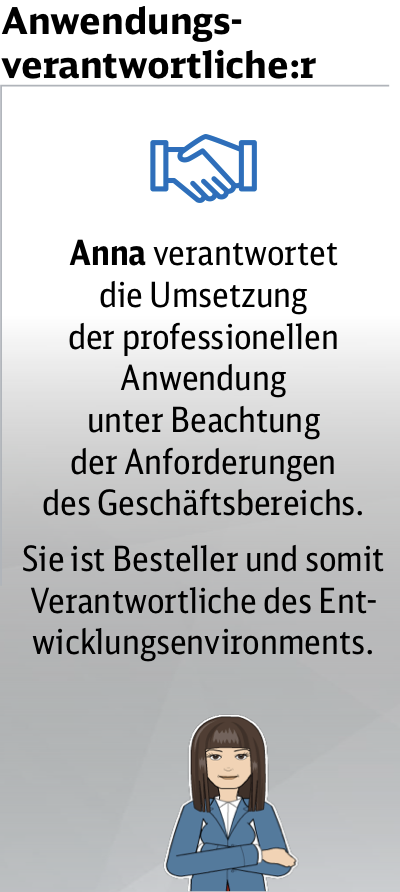
\includegraphics[scale = 0.3]{attachment/x_glossar/Scc003}
	\end{figure}
	}
}

\newglossaryentry{gDB_Enviromentverantwortliche(Maker)}{
	name={Anwendungsentwicklerin},
	description={
		Diese Person, wird durch die \gls{gDB_Anwendungsverantwortliche(Admin)}, in der Entwicklungsumgebung der Maker-Rolle zugewiesen. Diese ist für die Entwicklung der Anwendung oder des Flows zuständig.
	\begin{figure}[H]
		\centering
		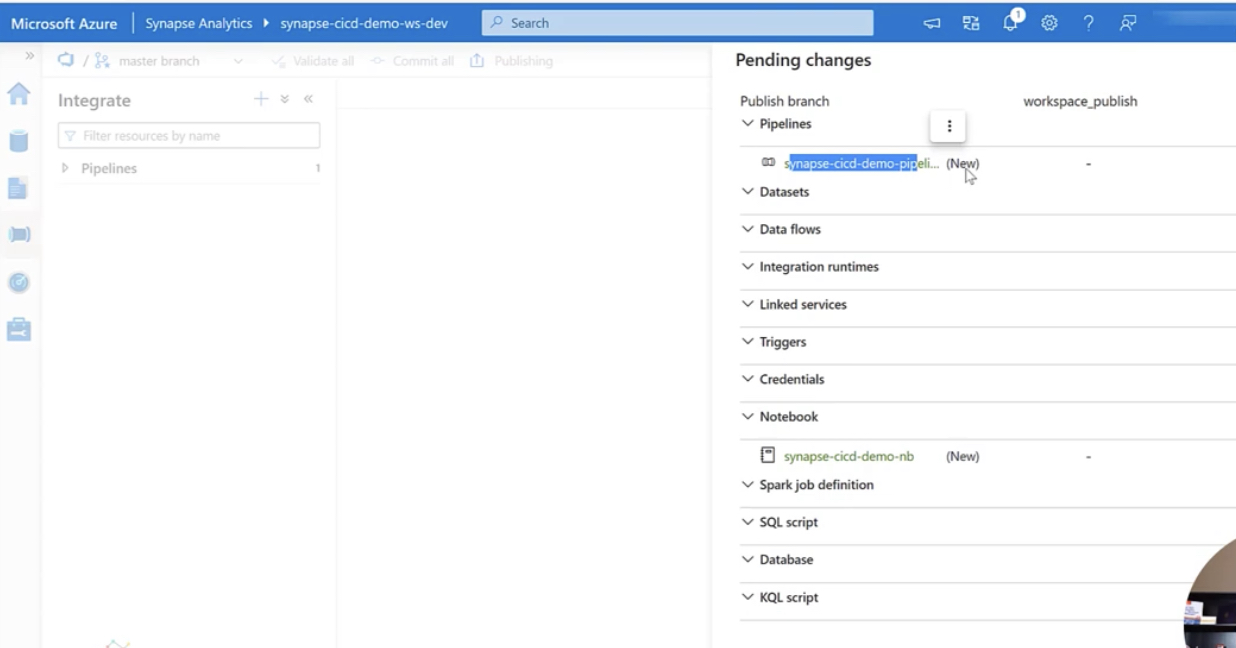
\includegraphics[scale = 0.3]{attachment/x_glossar/Scc151}
	\end{figure}
	}
}

\newglossaryentry{gDB_Enviromentverantwortliche(Admin)}{
	name={Enviromentverantwortliche/Mutli-Stage Verantwortliche},
	description={
			Diese Person hat die DB-Goverance und Prozessverantwortung. Sie überwacht die Hostung verschiedener Applikationen/ Flows in der Produktionsumgebung. Die Rolle wird der Person zu gewiessen, welche die \textit{Multi-Stage Umgebung} über das Digitalportal bestellt.
	\begin{figure}[H]
		\centering
		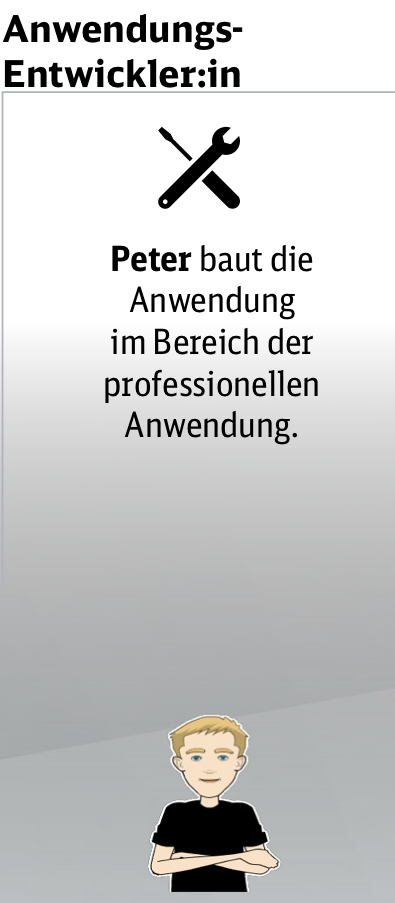
\includegraphics[scale = 0.3]{attachment/x_glossar/Scc001}
	\end{figure}
	}
} % Nicht mehr uptodate

%%%%%%%%%% Glossar %%%%%%%%%%%%%%%%

\newglossaryentry{g_Epoch}{
	name={Epoch},
	description={
	One epoch is when an ENTIRE dataset is passed forward and backward through the neural network only ONCE.
	}
}

\newglossaryentry{g_ONNX}{
	name={ONNX},
	description={
	Open Neural Network Exchange is an open ecosystem for AI models. It helps move you model with the different development cycle.
	}
}

\newglossaryentry{g_Measure}{
	name={Measure},
	description={
	Dies ist eine berechnenden DAX-Funktion. Dies ist zu unterscheiden zu den \textit{Berechneten Feld} Funktionen, die für Tabellen die nicht im Datenmodell enthalten sind, zu nutzen sind. 
	}
}

\newglossaryentry{g_Berechnende-Spalte}{
	name={Berechnende Spalte},
	description={
		Diese ergänzen Tabellen, welche im Datenmodell eingefügt sind. Dabei werden Daten erzeugt und auch im Arbeitsspeicher geladen. Diese Spalten lassen keine Aggregations zu und beziehen sich ausschließlich auf jede Zeile in einer Tabelle. 
	}
}

\newglossaryentry{g_IS}{
	name={Intellisense},
	description={
		Dies ist eine Anwendung zur Auto-Vervollständigung
	}
}

\newglossaryentry{g_API}{
	name={Application Programming Interface},
	description={
		Ein Programmschnittstelle ist eine Interaktionsmöglichkeit, die ein Programm anderen Programmen bietet auf bestimmte Teile der Software und oder Daten zuzugreifen.
	}
}

\newglossaryentry{g_ODBC}{
	name={Open Database Connectivity (or Connector)},
	description={
		Es handelt sich hierbei um eine API Verbindung zu einem DBMS.
		Das Ziel ist, dass eine Datenverbindung zu Datenbanksystem hergestellt werden kann, die unterschiedlicher Natur und oder auf unterschiedlichen Plattformen laufen. 
	}
}

\newglossaryentry{g_QlikSense}{
	name={Qlik Sense},
	description={
		Qlik Sense ist eine Business Analytics Software, welche die QlX-Engine Technologie nutzt.
	}
}

\newglossaryentry{g_M}{
	name={M Formula Language},
	description={
		Power Query nutzt die Sprache M. Diese ist eine funktional Sprache ähnlich zu F. Es können mit den Ausdrücken Daten gefiltert und transformiert werden.
	}
}

\newglossaryentry{g_SQLite}{
	name={SQLite},
	description={
		SQLite ist ein relationales Datenbanksystem. 
	}
}

\newglossaryentry{g_SQL}{
	name={SQL},
	description={
		\gls{SQL} ist eine Sprache welche strukturierte Abfragen an Datenbanken stellt. Diese Sprache wird von Datenbanken wie MySQL, Oracle, Mircosoft SQL Server, etc. verwendet. 
	}
}

\newglossaryentry{g_Git}{
	name={Git},
	description={
		Git is a free and open-source distribution \gls{VCS}. It trackes changes in source code during software development.  
	}
}

\newglossaryentry{g_EC2}{
	name={Amazon Elastic Computing Cloud},
	description={
		Amazon Elastic Compute Cloud (Amazon EC2) bietet eine skalierbare Rechenkapazität in der Amazon-Web-Services(AWS)-Cloud. Amazon EC2 beseitigt die Notwendigkeit, im Voraus in Hardware investieren zu müssen. Daher können Sie Anwendungen schneller entwickeln und bereitstellen. Sie können Amazon EC2 verwenden, um so viele oder so wenige virtuelle Server zu starten, wie Sie benötigen, Sicherheit und Netzwerk zu konfigurieren und den Speicher zu verwalten. Amazon EC2 können Sie auf- oder abwärts skalieren, um auf geänderte Anforderungen oder Datenverkehrsspitzen zu reagieren. Dies reduziert die Notwendigkeit, den Datenverkehr vorauszusagen.
	}
}

\newglossaryentry{g_Git_Repository}{
	name={Git Repository},
	description={
		Repositories in GIT contain a collection of files of various different versions of a Project. These files are imported from the repository into the local server of the user for further updations and modifications in the content of the file. A \gls{VCS} or the Version Control System is used to create these versions and store them in a specific place termed as a repository \cite{Geeks.2020}.  
	}
}

\newglossaryentry{g_Git_CMD}{
	name={Git Repository},
	description={
		Repositories in GIT contain a collection of files of various different versions of a Project. These files are imported from the repository into the local server of the user for further updations and modifications in the content of the file. A \gls{VCS} or the Version Control System is used to create these versions and store them in a specific place termed as a repository \cite{Geeks.2020}.  
	}
}

\newglossaryentry{g_Shell}{
	name={Shell},
	description={
		Eine Shell ist ein Befehl Interprator (Commandline Interpretar). Diese gibt Zugang zum Betriebssystem. Im Regelfall wird dieser über ein command-line or graphical user interface gesteuert.
	}
}

\newglossaryentry{g_Python}{
	name={Python},
	description={
		Python is an interpreted, high-level and general-purpose programming language. Python's design philosophy emphasizes code readability with its notable use of significant whitespace. \cite{wiki.pyh}
	}
}

\newglossaryentry{g_HTTP}{
	name={HTTP},
	description={
		The Hypertext Transfer Protocol is an application layer protocol for distributed, collaborative, hypermedia information systems. HTTP is the foundation of data communication for the World Wide Web, where hypertext documents include hyperlinks to other resources that the user can easily access, for example by a mouse click or by tapping the screen in a web browser. \cite{wiki.HTTP}
	}
}

\newglossaryentry{g_URL}{
	name={URL},
	description={
	A Uniform Resource Locator (URL), colloquially termed a web address, is a reference to a web resource that specifies its location on a computer network and a mechanism for retrieving it. A URL is a specific type of Uniform Resource Identifier (URI), although many people use the two terms interchangeably. URLs occur most commonly to reference web pages (http), but are also used for file transfer (ftp), email (mailto), database access (JDBC), and many other applications. \cite{wiki.URL}
	}
}

\newglossaryentry{g_JSON}{
	name={JSON},
	description={
		JavaScript Object Notation strukturiert Daten. Dieses Datenformat hat sich in der Webentwicklung verbreitet. Bei Anfragen von Rest-API kann man ein JSON Format erwarten. Ebenso finden JSON-Formate in Log und Confi-Datein ihren Nutzen.
		Es gibt 6 Datenformate, welche in einer JSON Datei abgespeichert werden können. String, Boolom, Integer, null, Array und Object
	} 
}

\newglossaryentry{g_NULL}{
	name={NULL (R)},
	description={
		In \gls{CPP} oder R wird \textit{NULL} verwendet, wenn Variablen deklariert werden. Der Pointer zeigt auf \textit{NULL}, und die Variablen bleiben vorherst leer: \textit{int height;}.
	} 
}

\newglossaryentry{g_None}{
	name={None},
	description={
		None ist ählich zu NULL. Es ist ein eigener Datentype: NoneType. Dieser Datentyp kann nur einen Wert besitzten \textit{None}. Zum Vergleich Integer kann Werte von $-3, 2, 10, \dots$ besitzen. Aus diesem Grund ist $None == None$ \textit{true}. Ebenso ist $None$ \textit{is} $None$ \textit{true}, weil es nur ein Objekt gibt, welches diesen Wert besitzt.
		In Python werden Varialben \underline{nicht} zuerst deklariert. Diese bedeuetet, diese halten immer eine Wert in dem entsprechenden Typ.
		Funktionen, welche keinen Rückgabewert wieder geben, nutzen \textit{None}: def no-return(void): pass $\rightarrow$ print(no-return):\textit{None}. Die normale Ausgabe der Funktion zeigt nicht an. Diese hat damit zu tun, dass Python dies unterdrückt.\\
		Die Instanz \textit{None} gibt es in Python nur einmal, wird mehrere Objekte \textit{None} zugewiesen, so zeigen alle Objekte, auf die selbe Instanz. \footnote{\href{https://medium.com/analytics-vidhya/dealing-with-missing-values-nan-and-none-in-python-6fc9b8fb4f31}{Link}}
	} 
}

\newglossaryentry{g_NaN}{
	name={NaN},
	description={
		NaN ist eine numerische Fehlerabfrage. Es ist ein besonder \textit{floot}-Zeiger. Dieser kann aus verschiedensten Gründen auftretten. Der Unterschied zu None ist, dass None bewusst definiert und ausgegeben wird - ähnlich zu Null. Bei NaN handelt sich sich um ein Float wert, der aus den verschiedensten Gründen entstehen kann, immer aber eine Sackgasse representiert, weil von NaN zu anderen Werten nicht transformiert werden kann - Virusbefall von Daten.\\
		Aus diesem Grund ist ein Vergleich von zwei NaN Ausgaben auch nicht zwangläufig gleich, weil die interne Kodierung von Fall zu Fall unterscheidlich ist. Es kann ebenso sein, dass die Sprache NaN direkt definiert - wie in Python, dass eine Gleichungs-Abfrage $NaN==NaN \rightarrow$ \textit{false} zurückgibt. Dies würde dann bedeuten, selbst wenn der Fehlercode der gleiche ist, würde \textit{false} zurückgegeben. \\
		Was die Identität $id()$ angeht, sind Variablen mit $np.nan$ gleiche Objekte. Zwischen Dataframe erstellt NaN, NumPy, Math, Etc. können und sind meistens die Objekt-Identitäten anderen, weshalb eine Abfragen von Dataframe erstellten NaN und NumPy NaN nicht in $true$ sondern $false$ resultiert. %\footnote{\href{Webseite}{https://towardsdatascience.com/navigating-the-hell-of-nans-in-python-71b12558895b}}
	} 
}

\newglossaryentry{g_Na}{
	name={Na (R)},
	description={
		In R exitiert zu NULL und NaN auch Na. Es handelt sich hier um einen logischen Operator. Die Besonderheit ist, dass dieser, wenn abgefragt, $Na$ zurückgibt. $Na=Na \rightarrow Na$. Dieser Operator kann in verschieden Datetypen: Array, Vektor, Matrix, etc. vorkommen.
		\footnote{\href{https://www.r-bloggers.com/2018/07/r-null-values-null-na-nan-inf/}{Link 2}\href{https://www.r-bloggers.com/2010/04/r-na-vs-null/}{Link}}
	} 
}

\newglossaryentry{g_scikit}{
	name={scikit learn},
	description={
		Es enthält sich um ein Packet, welches Algorithmen für maschninielles Lernen in Python beinhalten. Fragestellungen aus dem Data Scince Bereich können damit beantwortet werden. Ebenso enthält scikit learn zusätzliche Funktionen die bei Preprocessing, Feature Extraction, Evaluation und weiteres helfen.
		Dier Name setzt sich aus Science und Toolkit zusammen. Abgekürzt heißt es sklearn.
	} 
}

%%%%%% Stochastik 


\newglossaryentry{g_Stochastik}{
	name={Stochastik},
	description={
		Unter dem Feld der Stochastik wird die \textbf{Wahrscheinlichkeitstheorie} und die \textbf{Statistik} zusammengefasst. Der Begriff Stochastik bedeutet \textit{Kunst des Vermutens}. Zwei Schwerpunkt des Wahrscheinlichkeitslehre ist, zu modellieren, wie wahrscheinlich es ist das ein Ereignis eintritt und welche Ereignise es geben kann. Statistik hat den Schwerpunkt anhand von Daten Rückschlüsse auf Charakteristika eine wahrscheinlichkeitstheoritischen Modells zu ziehen.
	} 
}

\newglossaryentry{g_Statistik}{
	name={Statistik},
	description={
		Das Feld der Statistik ist ein Teilbereich der Stochastik. Der Schwerpunkt der Statistik ist, Datenmenge auszuwerten, zu interpretieren und wie diese verteilt sind.
	} 
}

\newglossaryentry{g_Wahrscheinlichkeitstheorie}{
	name={Wahrscheinlichkeitstheorie},
	description={
		Die Wahrscheinlichkeitstheorie, auch Wahrscheinlichkeitsrechnung oder Probabilistik, ist ein Teilgebiet der Mathematik, das aus der Formalisierung, der Modellierung und der Untersuchung von Zufallsgeschehen hervorgegangen ist.
	}
}

% Up
%%%%%% Stochastik 

\newglossaryentry{g_BuildArtifacts}{
	name={Build Artifacts},
	description={
		In Kurz: Environment + Compieled Output = Artifact. 
		In Lang: Die Umgebung mit alle Werkzeugen, Abhängikeiten, welche benötigt werden, um die Build (oder Image oder Source) plus tatsächlich compilierte resultate. Kommt es zu einem Fehler, ist alles an einem Ort, um unabhängig von den Konfigurationen, eine Fehleranalyse durchzuführen.
		Artifact kann auch nur $"$etwas produziertes$"$ bedeuteten. Somit ist \textit{libs/runnables - Compilied Artifacts}; \textit{Image - Build Step}.
	}
}

\newglossaryentry{g_conda}{
	name={conda},
	description={
		Pip installs Python packages whereas conda installs packages which may contain software written in any language. For example, before using pip, a Python interpreter must be installed via a system package manager or by downloading and running an installer. on the other hand can install Python packages as well as the Python interpreter directly.
	}
}

\newglossaryentry{g_pip}{
	name={pip},
	description={
		Package Installer for Python is the de facto and recommended package-management system written in Python and is used to install and manage software packages. It connects to an online repository of public packages, called the Python Package Index.
	}
}


\newglossaryentry{g_DataLake}{
	name={Data Lake},
	description={
		Es besteht die Chance, das Data Lake und Data Warehouse im gleichen Kontext verwendet werden. Diese beschreiben jedoch zwei unterschiedliche Konzepte.
		Ein Daten in einem Data Lake haben kein spezifischen Anwendungsfall, in welchen erkannt wird, in welchem diese genau benötigt werden. Ein Data Warehouse im Gegenzug hat einen initalen Anwendungsfall, welche eine genaue Verbindung zwischen Daten und der Anwendung erkennen lässt. In einem Data Lake werden die Daten unstrukturiert, ungefiltert und ohne einen Qualitätscheck abgelegt. Dies Daten werden von Data Scientist und Data Analyist herangezogen, um mit ML-Algorithmen neue Erkenntnisse zu gewinnen. Es handelt sich hierbei um eine neuere Technologie.
	}
}

\newglossaryentry{g_DataWarehouse}{
	name={Data Warehouse},
	description={
		Es besteht die Chance, das ein Data Warehouse und ein Data Lake im gleichen Kontext verwendet werden. Im Gegensatz zu einem Data Lake können die gespeicherten Daten einen eindeutigen Anwendungsfall zugeordnet werden. Die Daten werden bereinigt und stehen in verwendbarer Qualität zur Verfügung. Diese Daten werden meist von Business Analysten verwendet. Diese Technologie ist eine etablierte Technologie.
	}
}

\newglossaryentry{g_Objective(OKR)}{
	name={Objective (OKR)},
	description={
		Der Begriff \textbf{Objective} bezieht sich in diesem Kontext auf die OKR-Logik. Im Gegensatz zum militärischen Gebrauch im Englischen ist es hier ein wünschenswerter Zustand, der nicht zwingend eine eindeutige Zielerreichung voraussetzt. Dieser Zustand kann kontinuierlich angepasst und überprüft werden. Ein Beispiel: \textit{Mein Ziel ist, dass Deutschland ein demokratisches Land ist.} Was genau unter Demokratie verstanden wird, kann zu Beginn klar definiert sein, sich aber im Laufe der Zeit ändern und mit neuen Erkenntnissen abgeglichen werden.
		Daher ist es bei einem \textit{Objective} besonders wichtig, die \textit{Key Results} und \textit{Maßnahmen} präzise zu beschreiben. Diese definieren, welche Indikatoren den Erfolg messen oder den Fortschritt hin zum \textit{Objective} bestimmen. Die \textit{Maßnahmen} legen konkret fest, welche Schritte unternommen werden, um das \textit{Objective} letztendlich zu erreichen.
	}
}

\newglossaryentry{g_Kernel_Jy_Py}{
	name={Kernel (IPython/ Jupyter)},
	description={
		The IPython kernel (ipykernel) is a Jupyter Notebook (web-interface) kernel for Python execution. This kernel is used to execute Python notebook code.
	}
}

\newglossaryentry{g_Kernel_Jy}{
	name={Kernel (General Jupyter)},
	description={
		The kernel is in general a the engine to excute the markdown and compute commands in a Jupyter Notebook (web-interface). Aka Compution environment
	}
}

\newglossaryentry{g_PyI}{
	name={Python Interpreter},
	description={
		The Python interpreter is CPython and is written in C programming languages. The interpreter checks and anaylses the source code. This code gets transformed into byte and then bit code. After evaluating it, the output gets returned.
	}
}

\newglossaryentry{g_JupyterNotebook}{
	name={Jupyter Notebook (Web Interface)},
	description={
		A Jupyter Notebook is a web-interface for edition code and text. Colloaquialy the file type is called Jupyter Notebook too. Also Jupyter Notebook gets reference for the set of objects to run the web interace and the underlining substructruke like a kernel.
	}
}


%%%%%%%%%%%%%%%%%%%%%%%%%%%%%%%%%%%%%
%\glsaddall % Der Befehl fügt alle Glossary-Einträge in das Glossar ein.
\addbibresource{alongside/Citavi_Bib_1.bib} %% Einbinden der bib-Datei
%\addbibresource{alongside/Citavi_Bib-Own.bib} %% Einbinden der bib-Datei

%Used XeLaTex compiler
\begin{document}

%\begin{titlepage} % Suppresses displaying the page number on the title page and the subsequent page counts as page 1

	\raggedleft % Right align the title page
	
	\textcolor{mainone}{\rule{3pt}{\textheight}} % Vertical line
	\hspace{0.05\textwidth} % Whitespace between the vertical line and title page text
	\parbox[b]{0.75\textwidth}{ % Paragraph box for holding the title page text, adjust the width to move the title page left or right on the page
	%	\noindent % Icon
	%	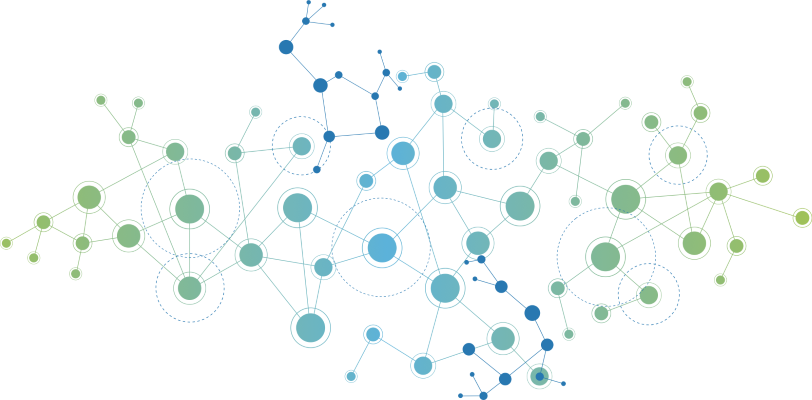
\includegraphics[scale=0.6]{attachment/Titel/point}\\
		
		\parbox[b]{0.57\textwidth}{
		
		\begin{center}
		\vspace{2cm}
		{\Large % Einleitung
			\bfseries 
			\textcolor{mainthree}{Notizen} \\[1\baselineskip]
		} 
	%	{\Huge  % Titel
		%	\textcolor{mainone}{\textbf{Data Science}}\\[\baselineskip]
	%	}
		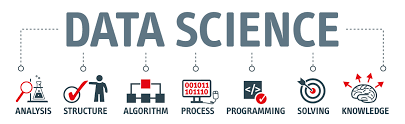
\includegraphics[width=0.9\linewidth]{attachment/x_titlepage/dsci} 
		{\Large % Untertitel mit Beschreibung
			\textit{Lernnotizen}\\
			[4\baselineskip] 
		}
	
		\vspace{4cm}
			{\Large
			\textsc{Paul Julitz}\\ % Author
		%	\vspace{1cm}
		%	vom 15. Oktober 2019 bis zum \today % Datum
		\vspace{0.3\textheight} 
	%	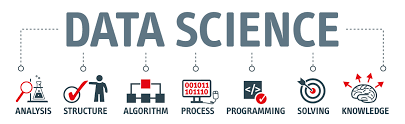
\includegraphics[width=0.6\linewidth]{attachment/x_titlepage/dsci}
		}\end{center}}
		
	
		%\noindent % Icon
	}
\end{titlepage}
	\begin{tikzpicture}[overlay,remember picture]
	
	\fill[black!2] (current page.south west) rectangle (current page.north east);
	
	\begin{scope}[transform canvas ={rotate around ={45:($(current page.north west)+(-.5,-6)$)}}]
		
		\shade[rounded corners=18pt, left color=maintwo, right color=maintwo!40] ($(current page.north west)+(-.5,-6)$) rectangle ++(9,1.5);
		
	\end{scope}
	
	\begin{scope}[transform canvas ={rotate around ={45:($(current page.north west)+(.5,-10)$)}}]
		
		\shade[rounded corners=18pt, left color=lightgray,right color=lightgray!60] ($(current page.north west)+(0.5,-10)$) rectangle ++(15,1.5);
		
	\end{scope}
	
	\begin{scope}[transform canvas ={rotate around ={45:($(current page.north west)+(0.5,-10)$)}}]
		
		\shade[rounded corners=8pt, left color=lightgray] ($(current page.north west)+(1.5,-9.55)$) rectangle ++(7,.6);
		
	\end{scope}
	
	\begin{scope}[transform canvas ={rotate around ={45:($(current page.north)+(-1.5,-3)$)}}]
		
		\shade[rounded corners=12pt, left color=mainone!80, right color=mainone!60] ($(current page.north)+(-1.5,-3)$) rectangle ++(9,0.8);
		
	\end{scope}
	
	\begin{scope}[transform canvas ={rotate around ={45:($(current page.north)+(-3,-8)$)}}]
		
		\shade[rounded corners=26pt, left color=red!80, right color=red!80] ($(current page.north)+(-3,-8)$) rectangle ++(15,1.8);
		
	\end{scope}
	
	\begin{scope}[transform canvas ={rotate around ={45:($(current page.north west)+(4,-15.5)$)}}]
		
		\shade[rounded corners=23pt, left color=mainone, right color=maintwo] ($(current page.north west)+(4,-15.5)$) rectangle ++(30,1.8);
		
	\end{scope}
	
	\begin{scope}[transform canvas ={rotate around ={45:($(current page.north west)+(13,-10)$)}},]
		
		\shade[rounded corners=20pt, left color=RoyalBlue ,right color=maintwo] ($(current page.north west)+(13,-10)$) rectangle ++(15,1.5);
		
	\end{scope}
	
	\begin{scope}[transform canvas ={rotate around ={45:($(current page.north west)+(18,-8)$)}},]
		
		\shade[rounded corners=8pt, left color=lightgray] ($(current page.north west)+(18,-8)$) rectangle ++(15,0.6);
		
	\end{scope}
	
	\begin{scope}[transform canvas ={rotate around ={45:($(current page.north west)+(19,-5.65)$)}},]
		
		\shade[rounded corners=12pt, left color=lightgray] ($(current page.north west)+(19,-5.65)$) rectangle ++(15,0.8);
		
	\end{scope}
	
	\begin{scope}[transform canvas ={rotate around ={45:($(current page.north west)+(20,-9)$)}}]
		
		\shade[rounded corners=20pt, left color=mainone, right color=red!80] ($(current page.north west)+(20,-9)$) rectangle ++(14,1.2);
		
	\end{scope}
	
	%% <> | <>
	% Draw Line
	\draw[ultra thick,gray] ($(current page.center)+(7,2.5)$) -- ++(0,-1.5cm) 

	node[midway,right=0.25cm,text width=5cm,align=left,black!75]{
	% Right part
	{
		\fontsize{15}{30} \selectfont  Study \\ [5pt] 
	}{
%		\center \fontsize{10}{40} \selectfont $\&$ and then \\[10pt] 
	}{
		\fontsize{15}{30} \selectfont $\&$ Research 
	}
	% Left part
	} node[midway,left=0.25cm,text width=6cm,align=right ,mainone]{
		{
			\fontsize{40}{86.4} \selectfont DSci
		}
	};

	%% Subtitle
	\node[text width=12cm,align=center] at ($(current page.center)+(0,-1)$) {
		{
			\fontsize{12}{19} \selectfont \textcolor{mainone}{
				\bf Data Science Journey
			}
		}	 
	};

	%%% Title
	% Section 1
	\node[text width=10cm, align=center] at ($(current page.center)+(4.5,-6)$) {
		{ % Text wrapper will take into account single letters size. For example "p" needs more space in the secound line, then "a".
			\fontsize{50}{52} \selectfont  Computer \linebreak  Science
		} 
	};
	% Section 2
	\node[text width=10cm, align=center] at ($(current page.center)+(0,-2.5)$) {

		{
			\fontsize{50}{52} \selectfont  Mathematics
		}
	};
	% Section 3
	\node[text width=10cm, align=center] at ($(current page.center)+(-4.5,-6)$) {
		{ % Text wrapper will take into account single letters size. For example "p" needs more space in the secound line, then "a".
			\fontsize{50}{52} \selectfont Domain \\ [9pt]  Knowledge
		}
	};
	%%% Title Connection Lines
	% Math-Domain Knowledge
	\draw[ultra thick,gray] (5,-15.5) -- (4.5,-16.5);
	% Math-Computer Sc
	\draw[ultra thick,gray] (10.5,-15.5) -- (11,-16.5);
	% Domain-Computer Sc
	\draw[ultra thick,gray] (7,-18) -- (8.5,-18);
	
	
	%% Extra Notes: Journey Description
	\node[text width=12cm,align=center] at ($(current page.center)+(0,-10)$) {
		{
			\fontsize{16}{19.2} \selectfont \textcolor{mainone}{
				\bf \difftoday{2020}{01}{03}
			 }
		}\\[3pt]
		{
			since the start of the journey on 3 January 2020.
		}	 
 };
	
\end{tikzpicture} 

\pagebreak
\hypersetup{linkcolor=black}
\tableofcontents
\pagebreak


%% Artifical Intelligence %%%%%%%%%%%%%%%%%%%%%%%%%
\part{Artificial Intelligence}
%%%%%%%%%%%%%%%%%%%%%%%%%%%%%%%%%%%%%%%%%%%%%%%%%%%

%\section{Libraries for Data Analysis}
\subsection{Working with Excel}
\subsubsection{Basic Pandas}
Im folgenden werden zwei Pakete benötigt: \textit{Pandas} und \textit{openpyxl}. \\
\begin{lstlisting}[style=python]
	import pandas as pd
	form openpyxl.workbook import Workbook
\end{lstlisting}
Panda ist ein freie Daten Analyse Bibliothek. Bei \textit{openpyxl} handelt es sich um eine Bibiliothek, welche das Lesen und Schreiben von Excel Dateien ermöglicht.\\

Pandas nutzt die folgenden Konzepte um Daten zu speichern und zu manipulieren:
\begin{description}
	\item[Dataframe] Dies wird genutzt, um 2D Tabellen abzuspeichern. 
	\item[Series] Dieses wird genutzt, um 1D Arrays abzuspeichern.
	\item[Panals] Diese wird genutzt, um 3D Daten abzuspeichern.
\end{description}

\paragraph*{pd.read()}
Die Funktion \textit{.read} importiert Daten in den Dataframe. Für verschiedenen Dateiformate bietet Panda unterschiedliche \textit{.read} Funktionen an:
\begin{figure}[H]
	\centering
	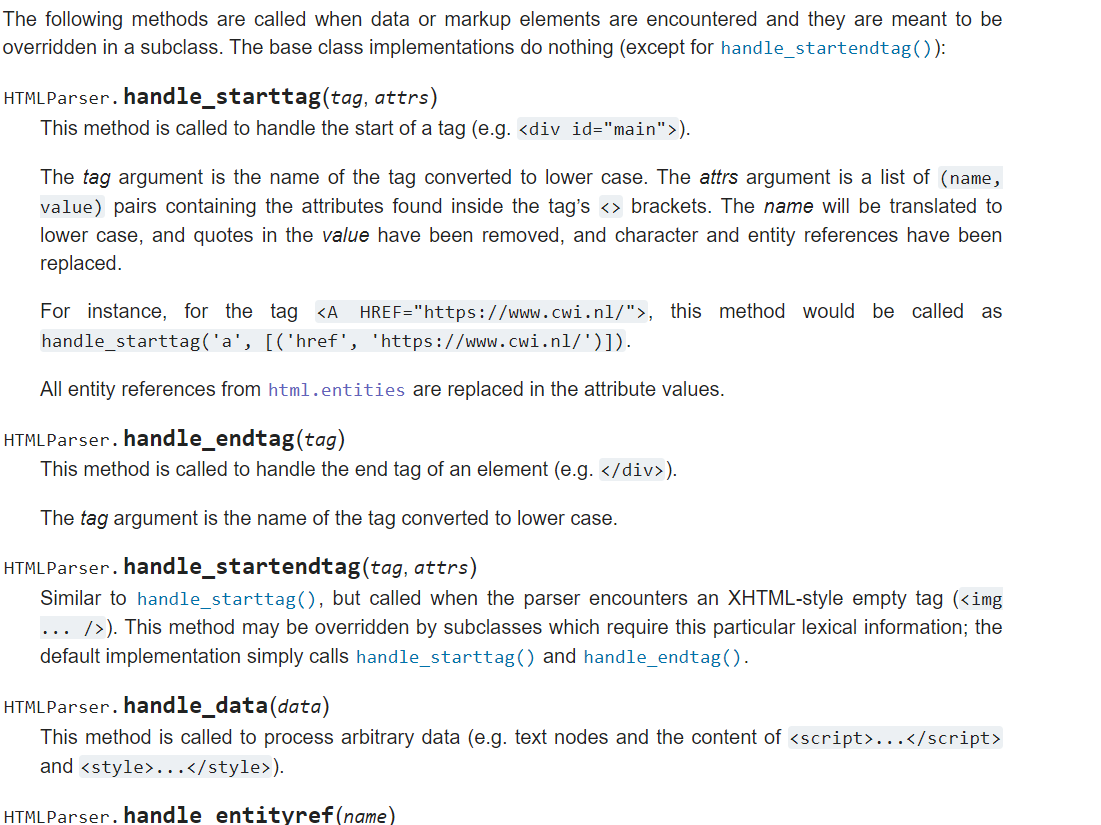
\includegraphics[scale = 0.3]{attachment/chapter_3/Scc077}
\end{figure} 

Das Paket \textit{xlrd} wird benötigt, um die \gls{xlsx} Formate einzulesen. Alternativ kann auch \textit{openpyxl} verwendet werden, um die Dateien einzulesen.
\begin{lstlisting}[style=python]
	# Import Data to Dataframe
	df_excel = pd.read_excel("regions.xlsx",engine='openpyxl')
	# The engine openpyxl was manuell added and installed. Also the Package xlrd was installed in iOS.
	df_csv = pd.read_csv("Names.csv")
	df_text = pd.read_csv("data.txt", delimiter="\t")
\end{lstlisting}

Beim Darstellen der Inhalte werden die ersten fünf und letzten fünf Zeilen ausgewiesen.
\begin{lstlisting}[style=python]
	#                ID  EGF_Baseline  EGF_Stimulus
	#0      FBgn0029994         -1.25         -0.27
	#1      FBgn0037191         -1.05          0.78
	#2      FBgn0036810          2.08          1.34
	#3      FBgn0033320          1.15          0.45
	#4      FBgn0051156         -1.77         -0.76
	#...            ...           ...           ...
	#11761  FBgn0026136          0.57          1.23
	#11762  FBgn0037356          1.14         -0.95
	#11763  FBgn0038214         -1.86         -0.67
	#11764  FBgn0042110          1.49          0.43
	#11765  FBgn0034202         -1.32         -0.22
\end{lstlisting}

In \gls{ETL} Prozess einer \gls{csv} Datei kann wie folgt aussehen.
\begin{lstlisting}[style=python]
	# Extract, Transform and Load
	df_csv = pd.read_csv("Names.csv",header=None)
	df_csv.columns = ["Vorname", "Nachname", "Street", "City", "State", "Postcode", "Unkown"] # Has to be complete.
	df_csv.to_excel("modified.xlsx") # same directory
\end{lstlisting}

\paragraph*{Lambda Function}
Lambda ist eine Funktion, welche zu einer anonymen Funktion referiert.
\begin{align}
	\text{Lambda (Argumgents)}:\text{expression}
\end{align}
Für weiteres siehe iloc Lambda Function. 

\paragraph*{set index}
Mit der Index Funktion kann eine oder mehrere Spalten als Index ausgewählt werden. Ebenso kann verifiziert werden, ob es sich um einen eindeutigen Schlüssel handelt oder nicht.
\begin{lstlisting}[style=python]
	df_new = df_csv.set_index("State", verify_integrity=True)
	### Output
	print(df_new)
	# ValueError: Index has duplicate keys: Index(['NJ', 'SD'], dtype='object', name='State')
\end{lstlisting}
Ohne diese Einschränkung und mit einer anderen Indexspalte wird folgendes wiedergegeben.
\begin{lstlisting}[style=python]
	df_new = df_csv.set_index("Postcode")
	### Output
	print(df_new)
	#
	#                      Vorname  Nachname                            Street         City State  Income
	#Postcode
	#8074                     John       Doe                 120 jefferson st.    Riverside    NJ   45000
	#9119                     Jack  McGinnis                      220 hobo Av.        Phila    PA   18000
	#8075            John "Da Man"    Repici                 120 Jefferson St.    Riverside    NJ  120000
	#91234                 Stephen     Tyler  7452 Terrace "At the Plaza" road     SomeTown    SD   90000
	#298                       NaN  Blankman                               NaN     SomeTown    SD   30000
	#123       Joan "Danger", Anne       Jet               9th, at Terrace plc  Desert City    CO   68000
\end{lstlisting}
\paragraph*{str.split}
Die Splitfunktion zerlegt eine Spalte in ihre Komponenten.
Mit der expand Option wird jede benötigte Abtrennung dargestellt.
\begin{lstlisting}[style=python]
	df_new = df_csv.set_index("Postcode")
	df_new = df_new["Vorname"].str.split(expand=True)
	#df_new = df_new.Vorname.str.split(expand=True) # Same Result
	### Output
	print(df_new)
	#                0          1     2
	#Postcode
	#8074         John       None  None
	#9119         Jack       None  None
	#8075         John        "Da  Man"
	#91234     Stephen       None  None
	#298           NaN        NaN   NaN
	#123          Joan  "Danger",  Anne
\end{lstlisting}
Die erste Spalte wird übertragen, wenn dieser direkt einer andern Spalte zugewiesen wird.
\begin{lstlisting}[style=python]
	df_new = df_csv.set_index("Postcode")
	df_new.Vorname = df_new["Vorname"].str.split(expand=True)
	### Output
	print(df_new)
	#          Vorname  Nachname                            Street         City State  Income
	#Postcode
	#8074         John       Doe                 120 jefferson st.    Riverside    NJ   45000
	#9119         Jack  McGinnis                      220 hobo Av.        Phila    PA   18000
	#8075         John    Repici                 120 Jefferson St.    Riverside    NJ  120000
	#91234     Stephen     Tyler  7452 Terrace "At the Plaza" road     SomeTown    SD   90000
	#298           NaN  Blankman                               NaN     SomeTown    SD   30000
	#123          Joan       Jet               9th, at Terrace plc  Desert City    CO   68000
\end{lstlisting}

\paragraph*{.replace}
Mit der replace Funktion wird ein Wert durch einen anderen Wert ersetzt. Die Konstante np.nan (Convert a string or number to a floating point number, if possible.) gibt Wahr oder Falsch wieder, wenn ein leerer Eintrag existiert.

\begin{lstlisting}[style=python]
	df_new = df_csv.set_index("Postcode")
	df_new.Vorname = df_new["Vorname"].str.split(expand=True)
	df_new = df_new.replace(np.nan, "NaN")
\end{lstlisting}
\subsubsection{Dataframe Functions}
Anhand des Beispiel \textit{Names.csv}.
\begin{lstlisting}[style=python]
	#	               Vorname  Nachname                            Street         City State  Postcode  Unkown
	#	0                 John       Doe                 120 jefferson st.    Riverside    NJ      8074   45000
	#	1                 Jack  McGinnis                      220 hobo Av.        Phila    PA      9119   18000
	#	2        John "Da Man"    Repici                 120 Jefferson St.    Riverside    NJ      8075  120000
	#	3              Stephen     Tyler  7452 Terrace "At the Plaza" road     SomeTown    SD     91234   90000
	#	4                  NaN  Blankman                               NaN     SomeTown    SD       298   30000
	#	5  Joan "Danger", Anne       Jet               9th, at Terrace plc  Desert City    CO       123   68000
\end{lstlisting}
\paragraph{Basics}


\paragraph*{.columns()} weißt den Spalten neue Bezeichnungen zu.
\paragraph*{df.[]} selektiert ausgewählte Spalte, z. B.: .["Vorname"] aus.. Mit einem Array an Spalten [["Vorname"],["Nachname"]] werden mehrere Spalten ausgelesen. Wenn keine Spalte vorliegt, wird diese erzeugt, wenn ihr ein Wert zugewiesen wird. (.["Test"]="Test")

\paragraph*{df.[][]} selektiert im ersten Bereich die Spalte und im zweiten Bereich die Zeilen.
\paragraph*{df.index} Ließt die Index Vektor aus.
\paragraph*{df.drop()} Spalten können entfernt werden. Der Parameter \textit{inplace} gleich \textit{false} gibt, an ob eine Kopie erstellt werden soll. Wird daraufhin \textit{.print()} angewandt, wird der Dataframe ohne die Spalten angezeigt. Wird der Parameter auf \textit{true} gesetzt, so werden die Daten gelöscht.
\begin{lstlisting}[style=python]
	# Drop
	df_new = df_csv.drop(columns=["Postcode"])
	df_new = df_new.groupby(["State"]).mean()
	#Income
	#State        
	# NJ     82500
	# PA     18000
	# SD     30000
	#CO      68000
	#SD      90000
	#>>> 
\end{lstlisting}

\paragraph*{df.head()} Shows a preview

\paragraph*{df.groupby()} Die Spalte, welche gruppiert werden soll, wird hier angegeben. 
\begin{lstlisting}[style=python]
	### Group by
	df_names_modifierd = df_names_modifierd.groupby(["State"]) 
	# Object at 0x...
\end{lstlisting}
Ohne eine spezielle Operation bleibt es bei einem Objekt. Wird die Funktion \textit{.mean()} hinzugefügt, wird diese auf jede Spalte mit Integer angewendet.
\begin{lstlisting}[style=python]
	### Group by
	df_names_modifierd = df_names_modifierd.groupby(["State"]).mean()
	#	       Postcode   Income  Tax Percentage  Tax Amount
	#	State
	#	NJ      8074.5  82500.0            0.25     15000.0
	#	PA      9119.0  18000.0            0.25         0.0
	#	SD       298.0  30000.0            0.25         0.0
	#	CO        123.0  68000.0            0.25     17000.0
	#	SD      91234.0  90000.0            0.25     22500.0
\end{lstlisting}

\paragraph*{df.groupby().mean()} berechnet den Durchschnitt einer Spalte.
\begin{lstlisting}[style=python]
	### Group by
	df_names_modifierd = df_names_modifierd.groupby(["State"]).mean().sort_values("Tax Amount")		
	#       Postcode   Income  Tax Percentage  Tax Amount
	#	State
	#	PA      9119.0  18000.0            0.25         0.0
	#	SD       298.0  30000.0            0.25         0.0
	#	NJ      8074.5  82500.0            0.25     15000.0
	#	CO        123.0  68000.0            0.25     17000.0
	#	SD      91234.0  90000.0            0.25     22500.0
\end{lstlisting}
Wie oben gezeigt, kann die Spalte [Postcode] auch entfernt werden.

\paragraph*{df.apply}
Apply() bietet an, dass Funktionen auf den Dataframe angewandt werden. Diese können weiter auf Bereiche (Achsen) spezifiziert werden.
Mit der Lambda Funktion kann eine Funktion für jeden Eintrag definiert werden. Dabei ist eine genauer Definition nach den Achsen nicht relevant.
\begin{lstlisting}[style=python]
	mydict = [{'a': 1, 'b': 2, 'c': 3, 'd': 4},
	{'a': 100, 'b': 200, 'c': 300, 'd': 400},          
	{'a': 1000, 'b': 2000, 'c': 3000, 'd': 4000 }]
	df_num = pd.DataFrame(mydict)
	
	# Select
	df_new = df_num.apply(lambda x: x+2)
	#df_new = df_num.apply(lambda x: x + 2, axis=0) # Same Result
	#df_new = df_num.apply(lambda x: x + 2, axis=1) # Same Result
	
	# Output
	print(df_new)
	#      a     b     c     d
	#0     3     4     5     6
	#1   102   202   302   402
	#2  1002  2002  3002  4002
	#>>> 
\end{lstlisting}
Mit \textit{axis} 0 oder 1 wird die Funktion entlang der Spalten oder Zeilen durchgeführt. Dies
Mit 0 wird der definierte Funktionsausdruck entlang aller Zeile für jede Spalte durchgeführt. Mit 1 wird für jede Zeile über alle Spalten gerechnet.\\
Für eine Auswahl an Funktion kann das Paket \textbf{numpy} geladen werden.\\

Aggrationen können entlang einer Achse durchgeführt werden. Zurückgegeben wird ein Array. Als default wird die Achse 0 ausgewählt.
\begin{lstlisting}[style=python]
	# Select
	df_new = df_num.apply(np.sum)
	### Output
	print(df_new)
	#a    1101
	#b    2202
	#c    3303
	#d    4404
\end{lstlisting}

Soll entlang einer Zeile die Funktion angewandt werden, wird Achse 1 ausgewählt.
\begin{lstlisting}[style=python]
	# Select
	df_new = df_num.apply(np.sum, axis=1)
	### Output
	print(df_new)
	#0       10
	#1     1000
	#2    10000
\end{lstlisting}

Um Berechnungen an bestimmten Spalten durchzuführen, werden diese an an neue übergeben.
\begin{lstlisting}[style=python]
	# Select
	df_csv["Tax Percentage"] = df_csv["Income"].apply(lambda x: .15 if 0 < x < 10000 else .30 if 10000 <= x < 30000 else .45)
	# if-then-else in one line has change to value_when_true if condition else value_when_false
	df_new = df_csv
	### Output
	print(df_new)
	#               Vorname  Nachname                            Street         City State  Postcode  Income  Tax Percentage
	#0                 John       Doe                 120 jefferson st.    Riverside    NJ      8074   45000            0.45
	#1                 Jack  McGinnis                      220 hobo Av.        Phila    PA      9119   18000            0.30
	#2        John "Da Man"    Repici                 120 Jefferson St.    Riverside    NJ      8075  120000            0.45
	#3              Stephen     Tyler  7452 Terrace "At the Plaza" road     SomeTown    SD     91234   90000            0.45
	#5  Joan "Danger", Anne       Jet               9th, at Terrace plc  Desert City    CO       123   68000            0.45
\end{lstlisting}

Eine Berechnung von zwei Spalten wird durch direktes Aufrufen durchgeführt.
\begin{lstlisting}[style=python]
	# Select
	df_csv["Tax Percentage"] = df_csv["Income"].apply(lambda x: .15 if 0 < x < 10000 else .30 if 10000 <= x < 30000 else .45)
	df_csv["Tax Amount"] = df_csv["Tax Percentage"]*df_csv["Income"]
	df_new = df_csv
	### Output
	print(df_new)
	#               Vorname  Nachname                            Street         City State  Postcode  Income  Tax Percentage  Tax Amount
	#0                 John       Doe                 120 jefferson st.    Riverside    NJ      8074   45000            0.45     20250.0
	#1                 Jack  McGinnis                      220 hobo Av.        Phila    PA      9119   18000            0.30      5400.0
	#2        John "Da Man"    Repici                 120 Jefferson St.    Riverside    NJ      8075  120000            0.45     54000.0
	#3              Stephen     Tyler  7452 Terrace "At the Plaza" road     SomeTown    SD     91234   90000            0.45     40500.0
	#4                  NaN  Blankman                               NaN     SomeTown    SD       298   30000            0.45     13500.0
	#5  Joan "Danger", Anne       Jet               9th, at Terrace plc  Desert City    CO       123   68000            0.45     30600.0
\end{lstlisting}

\paragraph{iloc - Index Number Locator}
Die Methode \textit{iloc[]} oder kurz loc filtert einen Datensatz nach Zeilen und Spalten. Dies Auswahl kann jedoch nur über den jeweiligen zu adressierten Index passieren. Die Berechnungszeit für iloc ist schneller als für loc, genau aus dem Grund, dass die Zeilen und Spalten schon geordnet sind, und somit leichter zu durchsuchen sind.
\paragraph*{Slicer Object} 
Im ersten Beispiel werden alle Zeilen (erste Eingabe vor dem Komma) ausgewählt. Der zweite Eintrag gibt die an, dass alle Spalten bis zur ersten ausgewählt werden sollen. Damit werden beide Achsen gefiltert.
\begin{lstlisting}[style=python]
	df_new = df_csv.iloc[:,:1]
	print(df_new)
	### Output
	#	               Vorname
	#0                 John
	#1                 Jack
	#2        John "Da Man"
	#3              Stephen
	#4                  NaN
	#5  Joan "Danger", Anne
	#>>> 	
\end{lstlisting}

Mit der Änderung auf 3 werden alle Spalten bis einschließlich der dritten Spalte gefiltert.
\begin{lstlisting}
	df_new = df_csv.iloc[:,:3]
	print(df_new)
	### Output
	#	               Vorname  ...                            Street
	#0                 John  ...                 120 jefferson st.
	#1                 Jack  ...                      220 hobo Av.
	#2        John "Da Man"  ...                 120 Jefferson St.
	#3              Stephen  ...  7452 Terrace "At the Plaza" road
	#4                  NaN  ...                               NaN
	#5  Joan "Danger", Anne  ...               9th, at Terrace plc
	#
	#[6 rows x 3 columns]
	#>>> 
\end{lstlisting}
Das Slicer Object kann auch mit einem booleschen Array kombiniert werden. Die Länge des Arrays muss gleich der Länge der zweiten Achse sein.
\begin{lstlisting}[style=python]
	# Select 
	df_new = df_csv.iloc[:,[True, False, False,False,False,False,False]]
	#   Nachname             Street
	#0       Doe  120 jefferson st.
	#1  McGinnis       220 hobo Av.
\end{lstlisting}
Ebenso kann auch eine leere Lambda Funktion oder ein Array für die zweite Achse eingelesen werden.
\begin{lstlisting}[style=python]
	# Select 
	df_new = df_csv.iloc[:, [0, 2]]
	# df_new = df_csv.iloc[:, lambda x: [0,2]] # Same result
	print(df_new)
	### Output
	#               Vorname                            Street
	#0                 John                 120 jefferson st.
	#1                 Jack                      220 hobo Av.
	#2        John "Da Man"                 120 Jefferson St.
	#3              Stephen  7452 Terrace "At the Plaza" road
	#4                  NaN                               NaN
	#5  Joan "Danger", Anne               9th, at Terrace plc
\end{lstlisting}

\paragraph*{Scalar}
Wird Scaler als Eingabe übergeben, wird eine \textit{Series} wiedergegeben und nach Zeilen gefiltert.
\begin{lstlisting}[style=python]
	df_new = df_csv.iloc[1]
	print(df_new)
	### Output
	#
	#Vorname             Jack
	#Nachname        McGinnis
	#Street      220 hobo Av.
	#City               Phila
	#State                 PA
	#Postcode            9119
	#Income             18000
	#Name: 1, dtype: object
	#>>> 
\end{lstlisting}
Mit einem \textbf{zweiten Scaler} wird die Spalte (Achse) ausgewählt. Der Eintrag der Zelle wird wiedergegeben.
\begin{lstlisting}
	df_new = df_csv.loc[1,1] # Zeilen Index 1 (Zweite Zeile), Spalten Index 1 (Zweite Zeile)
	print(df_new)
	#McGinnis
\end{lstlisting}

\paragraph*{Booelen Array}
Wird eine logische Operation (==, <, >) auf eine bestimmt Spalte des Dataframes angewendet, so wird eine \textit{Series} zurückgegeben. Die Series hat die gleiche Länge wie die Tabelle selbst. 
\begin{lstlisting}[style=python]
	# Select 
	df_new = df_csv["State"]=="SD"
	print(df_new)
	### Output
	0    False
	1    False
	2    False
	3     True
	4    False
	5    False
	Name: State, dtype: bool
\end{lstlisting}

Damit die Abfrage genutzt werden kann, muss aus der Serie das Array ausgelesen werden.
\begin{lstlisting}[style=python]
	# Select
	ser_new = df_csv.["State"]=="SD"
	#df_new = df_csv.loc[ser_new]
	print(df_new)
	### Output
	#   Vorname Nachname                            Street      City State  Postcode  Income
	#3  Stephen    Tyler  7452 Terrace "At the Plaza" road  SomeTown    SD     91234   90000
	#4      NaN  Blankman                               NaN  SomeTown    SD       298   30000
\end{lstlisting}
Mit iloc kann nur ein Array von Boolschen Werten eingelesen werden. Dies Serie muss nur nach dem Array ausgewertet werden.
\begin{lstlisting}[style=python]
	# Select
	ser_new = df_csv.["State"]=="SD"
	#df_new = df_csv.iloc[ser_new.array] # Array gibt ein narray wieder.
	print(df_new)
	### Output
	#   Vorname Nachname                            Street      City State  Postcode  Income
	#3  Stephen    Tyler  7452 Terrace "At the Plaza" road  SomeTown    SD     91234   90000
	#4      NaN  Blankman                               NaN  SomeTown    SD       298   30000
\end{lstlisting}
Alternativ muss ein Array der Länge des Dataframes eingegeben werde.
\begin{lstlisting}[style=python]                          NaN  SomeTown    SD       298   30000
	# Select 
	df_new = df_csv.loc[[False,False,False,True,False,False]]
	#df_new = df_csv.iloc[[False,False,False,True,False,False]] # loc bietet die gleiche Eingabemöglichkeit
	print(df_new)
	### Output
	#   Vorname Nachname                            Street      City State  Postcode  Income
	#3  Stephen    Tyler  7452 Terrace "At the Plaza" road  SomeTown    SD     91234   90000
	#4      NaN  Blankman                               NaN  SomeTown    SD       298   30000
\end{lstlisting}

\paragraph*{List of Integers(Index)}
Über iloc können auch die Indizes direkt eingegeben werden. Dafür werden sie als Array eingespielt.
\begin{lstlisting}[style=python]
	# Select
	df_new = df_csv.iloc[[0,1,2]]
	print(df_new)
	### Output
	#      	 Vorname  Nachname             Street       City State  Postcode  Income
	#0           John       Doe  120 jefferson st.  Riverside    NJ      8074   45000
	#1           Jack  McGinnis       220 hobo Av.      Phila    PA      9119   18000
	#2  John "Da Man"    Repici  120 Jefferson St.  Riverside    NJ      8075  120000
\end{lstlisting}
Mit dem zweiten Eintrag wird die zweite Achse gefiltert.
\begin{lstlisting}[style=python]
	# Select
	df_new = df_csv.iloc[[0,1,2],[1,2]]
	print(df_new)
	### Output
	#   Nachname             Street
	#0       Doe  120 jefferson st.
	#1  McGinnis       220 hobo Av.
	#2    Repici  120 Jefferson St.
\end{lstlisting}
\paragraph*{iloc with Lambda Function}
Lambda ist eine Funktion, welche zu einer anonymen Funktion referiert.
\begin{align}
	\text{Lambda (Argumgents)}:\text{expression}
\end{align}
Eine Lambda Funktion kann ebenso mit iloc verwendet werden. Im folgenden Beispiel wird der Ausdruck Modular 2 auf die Indizes der Zeilen angewandt. Das Argument $x$ ist dabei der Dataframe selbst. Mit .index werden die Indizes ausgelesen. Jeder gerade Zeilen Index wird ausgewählt.
\begin{lstlisting}[style=python]
	# Select 
	df_new = df_csv.iloc[lambda x: x.index % 2 == 0]
	print(df_new)
	### Output
	#         Vorname  Nachname             Street       City State  Postcode  Income
	#0           John       Doe  120 jefferson st.  Riverside    NJ      8074   45000
	#2  John "Da Man"    Repici  120 Jefferson St.  Riverside    NJ      8075  120000
	#4            NaN  Blankman                NaN   SomeTown    SD       298   30000
\end{lstlisting}

\paragraph{loc - Index Name Locator}
\paragraph*{Slicer Object, Scalar, List of Name Integers}
Der Fokus der loc Funktion ist, das die Indexes eine String Bezeichnungen besitzen. Im folgenden Beispiel wurden die Indizes für Zeilen und Spalten mit Strings näher definiert.
\begin{lstlisting}[style=python]
	# Select 
	#df_new = df_csv.iloc[:, [0, 2]]
	df = pd.DataFrame([[1, 2], [4, 5], [7, 8]],
	index=['cobra', 'viper', 'sidewinder'],
	columns=['max_speed', 'shield'])
	
	df_new = df.loc["cobra"]
	print(df_new)
	### Output
	#max_speed    1
	#shield       2
	#Name: cobra, dtype: int64
\end{lstlisting}
\begin{lstlisting}[style=python]
	# Select 
	df = pd.DataFrame([[1, 2], [4, 5], [7, 8]],
	index=['cobra', 'viper', 'sidewinder'],
	columns=['max_speed', 'shield'])
	
	df_new = df.loc["cobra","max_speed]
	print(df_new)
	### Output
	#1
\end{lstlisting}
Für den Slicer lässt sich die Logik auch übertragen.
\begin{lstlisting}[style=python]
	# Select 
	df = pd.DataFrame([[1, 2], [4, 5], [7, 8]],
	index=['cobra', 'viper', 'sidewinder'],
	columns=['max_speed', 'shield'])
	
	df_new = df.loc["cobra": "sidewinder"]
	print(df_new)
	### Output
	#            max_speed  shield
	#cobra               1       2
	#viper               4       5
	#sidewinder          7       8
\end{lstlisting}

\paragraph*{Booelen Array/ Series}
Es gilt das gleich wie bei iloc, bis auf die Ergänzung, dass Abfragen mit einem Serie ebenfalls gefüllt werden kann.

\begin{lstlisting}[style=python]
	# Select 
	df_new = df_csv.loc[df_csv["State"]=="SD"]
	#df_new = df_csv.loc[[False,False,False,True,False,False]] # Same Result
	print(df_new)
	### Output
	#   Vorname Nachname                            Street      City State  Postcode  Income
	#3  Stephen    Tyler  7452 Terrace "At the Plaza" road  SomeTown    SD     91234   90000
\end{lstlisting}
Ergänzend kann auch eine bedingte Abfrage mit einer Spaltenauswahl getroffen werden.
\begin{lstlisting}[style=python]
	df = pd.DataFrame([[1, 2], [4, 5], [7, 8]],
	index=['cobra', 'viper', 'sidewinder'],
	columns=['max_speed', 'shield'])
	
	df_new = df.loc[df["max_speed"]>0, ["shield"]]
	print(df_new)
	### Output
	#            shield
	#cobra            2
	#viper            5
	#sidewinder       8
\end{lstlisting}

\paragraph*{Change spezific Values based on condition}
Im Abschnitt df.apply wurden Steuersätze eingefügt. Diese Beispiel soll dienen, wie genau Daten geändert werden.
\begin{lstlisting}[style=python]
	# Select
	df_csv["Tax Percentage"] = df_csv["Income"].apply(lambda x: .15 if 0 < x < 10000 else .30 if 10000 <= x < 30000 else .45)
	df_csv["Tax Amount"] = df_csv["Tax Percentage"]*df_csv["Income"]
	
	df_new = df_csv.drop(columns=["Street","City", "State", "Postcode"])
	df_new.loc[df_new["Tax Percentage"]<= .3, "Tax Amount"] = 0
	### Output
	print(df_new)
	#               Vorname  Nachname  Income  Tax Percentage  Tax Amount
	#0                 John       Doe   45000            0.45     20250.0
	#1                 Jack  McGinnis   18000            0.30         0.0
	#2        John "Da Man"    Repici  120000            0.45     54000.0
	#3              Stephen     Tyler   90000            0.45     40500.0
	#4                  NaN  Blankman   30000            0.45     13500.0
	#5  Joan "Danger", Anne       Jet   68000            0.45     30600.0
\end{lstlisting}


\subsubsection{openpyxl}

\paragraph{Load existing workbook}
Um bestehenden Excel Dokumente zu laden, wird das Paket \textit{load}$\_$\textit{workbook} benötigt.
\begin{lstlisting}[style=python]
	from openpyxl import load_workbook
	
	wb_load = load_workbook("regions.xlsx")
	output = wb_load.sheetnames
	
	# Print
	print(output)
	#['Sheet1']
\end{lstlisting}

\paragraph{Workbook}
Das Paket Workbook bietet die Möglichkeit Workbooks direkt im Arbeitsspeicher zu erstellen, ohne diese vorher gespeichert zu haben.
\begin{lstlisting}[style=python]
	from openpyxl import load_workbook
	from openpyxl import Workbook
	
	wb_load = load_workbook("regions.xlsx")
	
	# Create new Workbook
	wb_new = Workbook()
	
	# Create new Worksheets
	ws1 = wb_new.create_sheet("New Sheet2",1)
	ws0 = wb_new.create_sheet("Legende", 0)
	ws2 = wb_new.create_sheet("Vorletze",-1)
	
	output = wb_new.sheetnames
	
	# Print
	print(output)
	# ['Legende', 'Sheet', 'Vorletze', 'New Sheet2']
\end{lstlisting}
Die Funktion \textit{create}$\_$\textit{sheet} hat als zweiten optionalen Parameter die Reihenfolge definiert. Diese startet bei 0.
Den Titel eines Sheets kann direkt mit \textit{.title} abgefragt werden.

\begin{lstlisting}[style=python]
	print(wb_new["Legende"].title)
	print(ws0.title) 
	#Legende
	#Legende
\end{lstlisting}

Ebenso kann über alle Worksheets interiert werden.
\begin{lstlisting}[style=python]
	for ws in wb_new:
	print(ws.title)
	#Legende
	#Sheet
	#Vorletze
	#New Sheet2
\end{lstlisting}

Ein bestimmtes Worksheet zu bearbeiten, erfordert es das zugehörige Workbook zu aktivieren.
\begin{lstlisting}[style=python]
	wb_new.active
	ws1["A4"] = 4
	output = ws1["A4"].value
	# 4
	wb_new.save("regions_new.xlsx")
\end{lstlisting}

Um das Workbook zu speichern, wird die save() Funktion genannt.

\paragraph{Select}
Zellen, Zeilen und Spalten können direkt über den ausgewählten Sheet angesteuert werden. 
\begin{lstlisting}[style=python]
	#from openpyxl import Workbook
	#import openpyxl as op
	from openpyxl import load_workbook
	from openpyxl import Workbook
	
	wb_load = load_workbook("regions.xlsx")
	
	# Create new Workbook
	wb_new = Workbook()
	
	# Create new Worksheets
	ws1 = wb_new.create_sheet("New Sheet2",1)
	ws0 = wb_new.create_sheet("Legende", 0)
	ws2 = wb_new.create_sheet("Vorletze",-1)
	
	wb_load.active
	
	for i in wb_load:
	print(i.title)
	
	range = wb_load["Sheet1"]["A1": "B7"]
	
	for i in range:
	for j in i:0
	print(j.value)	
\end{lstlisting}

Es gibt ebenso eine Iteration Funktion für Zeilen und Spalten.
\begin{lstlisting}[style=python]
	#from openpyxl import Workbook
	#import openpyxl as op
	from openpyxl import load_workbook
	from openpyxl import Workbook
	
	wb_load = load_workbook("regions.xlsx")
	
	# Create new Workbook
	wb_new = Workbook()
	
	# Create new Worksheets
	ws1 = wb_new.create_sheet("New Sheet2",1)
	ws0 = wb_new.create_sheet("Legende", 0)
	ws2 = wb_new.create_sheet("Vorletze",-1)
	
	ws = wb_load.active
	
	for i in wb_load:
	print(i.title)
	
	range = ws.iter_rows(min_row = 1, max_row = 3, max_col = 3, values_only = True)
	
	for i in range:
	for j in i:
	print(j)
	### Output
	#Sheet1
	#Region
	#Units
	#Sales
	#South
	#54
	#332
	#North
	#20
	#110
	#>>>
	
	### Output without values_only = True
	#Sheet1
	#<Cell 'Sheet1'.A1>
	#<Cell 'Sheet1'.B1>
	#<Cell 'Sheet1'.C1>
	#<Cell 'Sheet1'.A2>
	#<Cell 'Sheet1'.B2>
	#<Cell 'Sheet1'.C2>
	#<Cell 'Sheet1'.A3>
	#<Cell 'Sheet1'.B3>
	#<Cell 'Sheet1'.C3>
	#>>>  	
\end{lstlisting}

\paragraph{Mutliple Sheets}
Es können mehre Dateien und mehrere Tabellenblätter ausgelesen werden.
\begin{lstlisting}[style= python]
	import pandas as pd
	import time
	start_time = time.time()
	
	# Load data
	df_1 = pd.read_excel("shifts.xlsx", sheet_name= "Sheet1", skiprows=2, engine='openpyxl', usecols=lambda x: 'Unnamed' not in x)
	df_2 = pd.read_excel("shifts.xlsx", sheet_name= "Sheet1", skiprows=2, engine='openpyxl', usecols=lambda x: 'Unnamed' not in x)
	df_3 = pd.read_excel("shift_3.xlsx", skiprows=2, engine='openpyxl', usecols=lambda x: 'Unnamed' not in x)
	
	df_4 = pd.concat([df_1, df_2, df_3])
	
	
	print(df_4)
	print("--- %s seconds ---" % (time.time() - start_time))
	### Output
	#    Shift  ... Units Sold
	#0       2  ...        157
	#1       2  ...         83
	#2       2  ...        180
	#3       2  ...        186
	#4       2  ...        117
	#..    ...  ...        ...
	#94      3  ...         42
	#95      3  ...        168
	#96      3  ...        132
	#97      3  ...        111
	#98      3  ...        151
	#
	#[299 rows x 6 columns]
	#--- 0.4967920780181885 seconds ---
	#>>> 
\end{lstlisting}
\paragraph{Store Data from Dataframe into Workbook}
Mit der Funktion dataframe-to-rows wird ein Dataframe in Zeilen zerlegt. Die Werte aus diesen können einzeln adressiert werden und spezifischen Zellen in einem Worksheet zugewiesen werden.

\subsection{Exploritory Data Analysis}

Das Konzept \gls{EDA} wird unterschiedlich verwendet. Diese dient, die zu verwendenden Daten zu verstehen.

\subsubsection{Overview} 
\begin{itemize}
	\item df.head()
	\item for col in df.columns
	\item df.tail()
	\item df.shape
	\item df.describe()
	\item df[].unique()
	\item df.nunique()
	\item df.drop()
\end{itemize}
Als Datenquelle werden die COVID Zahlen des \gls{RKI} mit \href{https://npgeo-corona-npgeo-de.hub.arcgis.com/datasets/dd4580c810204019a7b8eb3e0b329dd6_0}{Flat-File.}
Die Legende findet sich unter \href{https://npgeo-corona-npgeo-de.hub.arcgis.com/datasets/dd4580c810204019a7b8eb3e0b329dd6_0}{Legende-RKI}
\paragraph{head()}
Im ersten Schritt werden die ersten Zeilen angezeigt.
\begin{lstlisting}[style= python]
	import pandas as pd
	import numpy as np
	import seaborn as sb
	
	df_rki = pd.read_csv("RKI_COVID19.csv")
	
	print(df_rki.head())
	### Output
	#   ObjectId  ...      Altersgruppe2
	#0         1  ...  Nicht übermittelt
	#1         2  ...  Nicht übermittelt
	#2         3  ...  Nicht übermittelt
	#3         4  ...  Nicht übermittelt
	#4         5  ...  Nicht übermittelt
	#
	#[5 rows x 18 columns]
	#>>> 	
\end{lstlisting}
\paragraph{columns}
Die einzelnen Namen der Spalten werden über eine Iteration angezeigt.
\begin{lstlisting}[style=python]
	for col in df_rki.columns:
	print(col)
	### Output
	ObjectId
	IdBundesland
	Bundesland
	Landkreis
	Altersgruppe
	Geschlecht
	AnzahlFall
	AnzahlTodesfall
	Meldedatum
	IdLandkreis
	Datenstand
	NeuerFall
	NeuerTodesfall
	Refdatum
	NeuGenesen
	AnzahlGenesen
	IstErkrankungsbeginn
	Altersgruppe2
	>>> 
	
	# tail() shows the last five entries	
	print(df.tail())
	### Output
	#         ObjectId  ...      Altersgruppe2
	#1134991   1134992  ...  Nicht übermittelt
	#1134992   1134993  ...  Nicht übermittelt
	#1134993   1134994  ...  Nicht übermittelt
	#1134994   1134995  ...  Nicht übermittelt
	#1134995   1134996  ...  Nicht übermittelt
	#
	#[5 rows x 18 columns]
	#>>> 
\end{lstlisting}
\paragraph{describe()}
Die Funktion\textit{describe()} gibt einen Standardabfrage an den Dataframe wieder.
\begin{lstlisting}[style=python]
	df = pd.read_csv("RKI_COVID19.csv")
	df_a = df["Altersgruppe"]
	x = df_a.describe()
	print(x)
	### Output
	#
	#count     1134996
	#unique          7
	#top       A35-A59
	#freq       386139
	#Name: Altersgruppe, dtype: object
	#>>> 
\end{lstlisting}
Als nächstes wird ein Jupyter Auszug einfügt, in welcher weiter mit der describe() Funktion gearbeitet wird.

\begin{figure}[H]
	\centering
	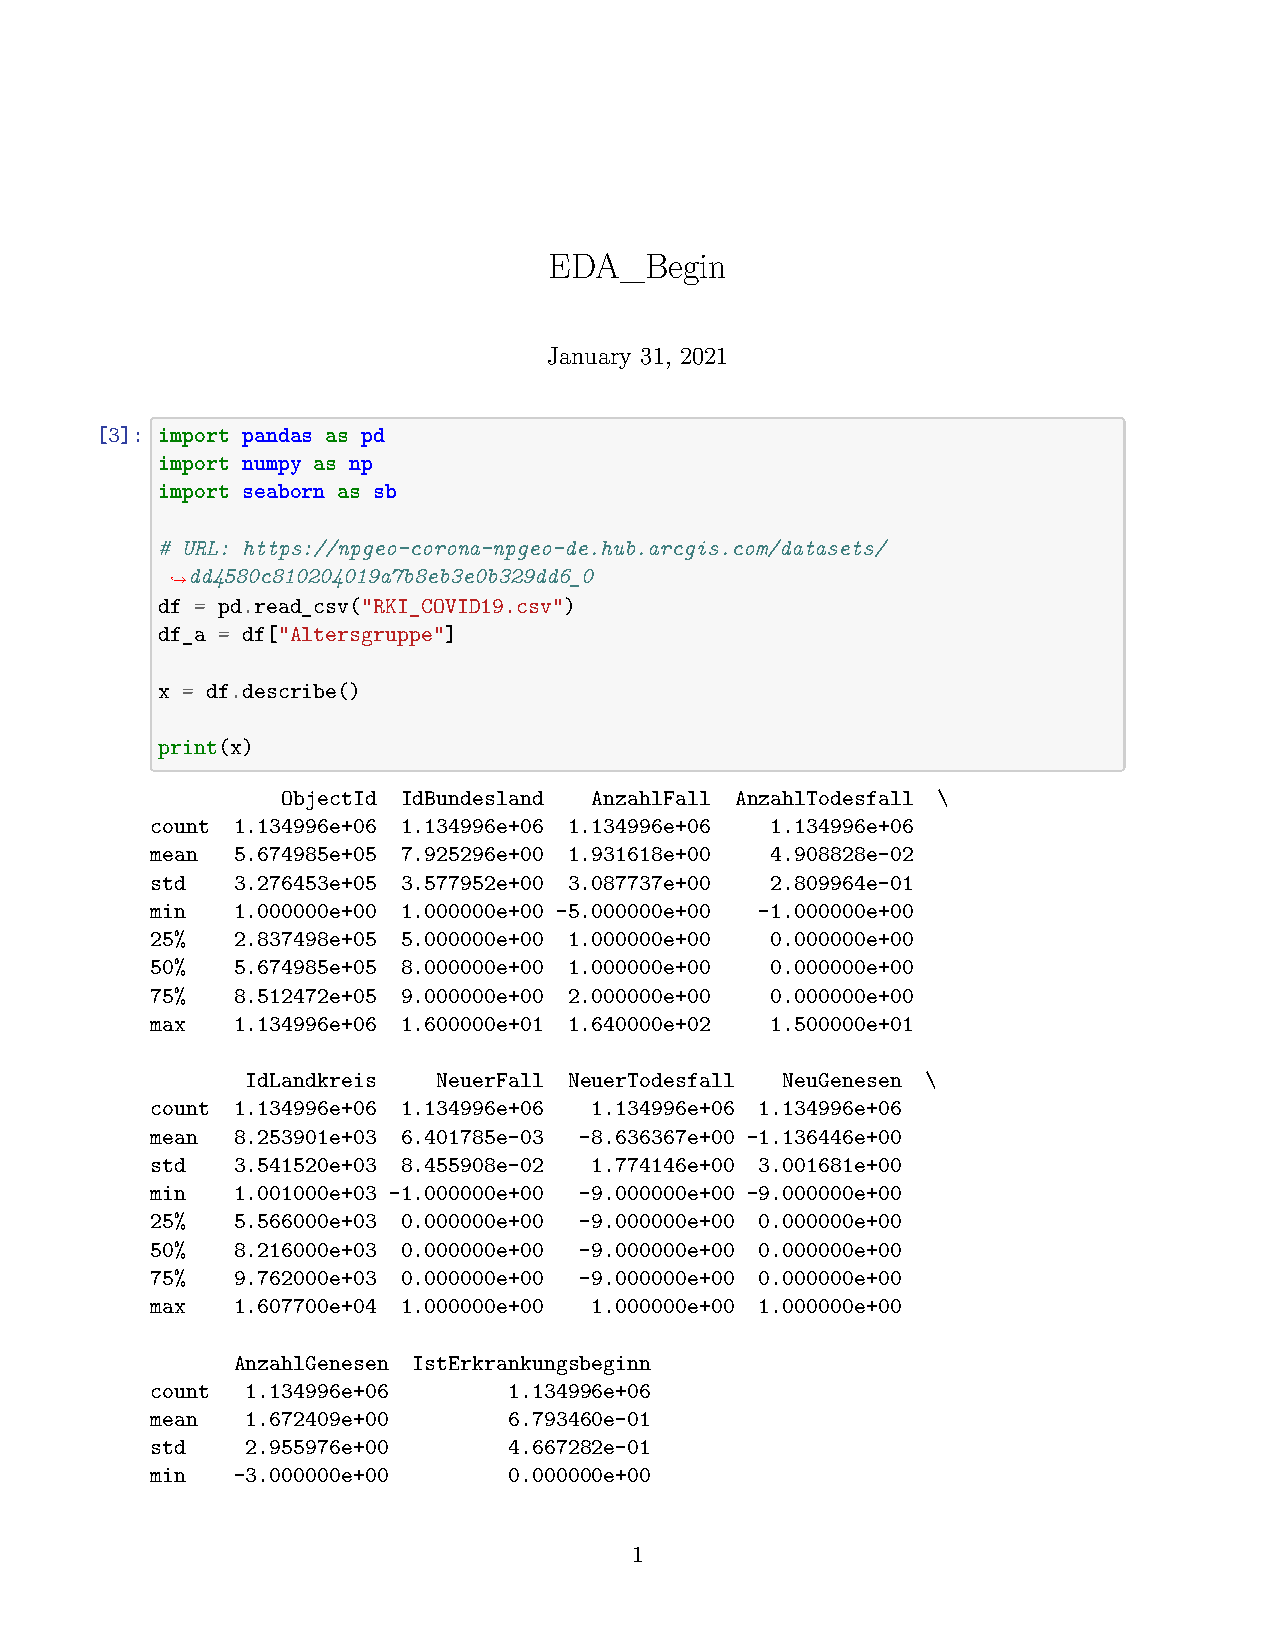
\includegraphics[scale = 0.8]{attachment/chapter_3/Scc078}
\end{figure} 

\paragraph{nunique() unique()}
Mit dieser Funktion werden alle Spalten abgegangen und die verschiedenen Werte wieder gegeben.
\begin{lstlisting}[style=python]
	df.nunique()
	ObjectId                1134996
	IdBundesland                 16
	Bundesland                   16
	Landkreis                   412
	Altersgruppe                  7
	Geschlecht                    3
	AnzahlFall                  128
	AnzahlTodesfall              16
	Meldedatum                  380
	IdLandkreis                 412
	Datenstand                    1
	NeuerFall                     3
	NeuerTodesfall                4
	Refdatum                    394
	NeuGenesen                    4
	AnzahlGenesen               127
	IstErkrankungsbeginn          2
	Altersgruppe2                 1
	dtype: int64
\end{lstlisting}
Sollen die Werte der jeweiligen Spalte ausgegeben werden, so bietet sich die Funktion unique() an.
\begin{lstlisting}[style=python]
	df["Geschlecht"].unique()
	array(['M', 'W', 'unbekannt'], dtype=object)
	df["NeuerFall"].unique()
	array([ 0, -1,  1], dtype=int64)
\end{lstlisting}

\paragraph{Check for Nullvalues}
In zwei Schritte kann eine Übersicht geschaffen werden, welche Ausschluss über die leere Werte im Dataframe gibt.
\begin{lstlisting}[style=python]
	df.isnull().sum()
	ObjectId                0
	IdBundesland            0
	Bundesland              0
	Landkreis               0
	Altersgruppe            0
	Geschlecht              0
	AnzahlFall              0
	AnzahlTodesfall         0
	Meldedatum              0
	IdLandkreis             0
	Datenstand              0
	NeuerFall               0
	NeuerTodesfall          0
	Refdatum                0
	NeuGenesen              0
	AnzahlGenesen           0
	IstErkrankungsbeginn    0
	Altersgruppe2           0
	dtype: int64
\end{lstlisting}
Mit Isnull() wird eine logische Überprüfung durchgeführt werden. Mit der Summe über alle Spalten wird die Menge der leeren Werte summiert angezeigt.

\paragraph{Convert Date as String to Date type}
Die übergebenen Datumswerte sind als String übergeben. Um diese filtern und weiter bearbeiten zu können, werde diese mit dem Paket \textit{datetime} umgewandelt.
\begin{lstlisting}[style=python]
	#%%
	import pandas as pd
	import numpy as np
	import seaborn as sb
	import datetime as dt
	
	# URL: https://npgeo-corona-npgeo-de.hub.arcgis.com/datasets/dd4580c810204019a7b8eb3e0b329dd6_0
	df = pd.read_csv("RKI_COVID19.csv")
	
	df_SKA = df.loc[df["Landkreis"]=="SK Augsburg"]
	df_SKA = df_SKA[["Meldedatum","AnzahlFall"]]
	df_SKA = df_SKA.iloc[0:3]
	df_SKA["Date"] = df_SKA["Meldedatum"].apply(lambda x: dt.datetime.strptime(x, '%Y/%m/%d %H:%M:%S')) # apply 
	df_SKA["year"] = df_SK["Date"].apply(lambda x: x.year)
	df_SKA["Month"] =  df_SKA["Date"].apply(lambda x: x.month)
	df_SKA["Day"] =  df_SKA["Date"].apply(lambda x: x.day)
	df_SKA.drop(["Meldedatum"], axis=1, inplace=True) # inplace modifize the same variable
	df_SKA.head()
	
	# %%
	#AnzahlFall	Date	year	Month	Day
	#845500	1	2020-09-13	2020	9	13
	#845503	1	2020-05-28	2020	5	28
	#845504	1	2020-05-31	2020	5	31
\end{lstlisting}

\paragraph{Histogramm}
Anteil der Infektionen:
\begin{lstlisting}[style=python]
	#%%
	import pandas as pd
	import numpy as np
	import seaborn as sb
	import datetime as dt
	
	# Source
	# URL: https://npgeo-corona-npgeo-de.hub.arcgis.com/datasets/dd4580c810204019a7b8eb3e0b329dd6_0
	df_SKA = pd.read_csv("RKI_COVID19.csv")
	
	#Select Data for Augsburg
	df_SKA = df_SKA.loc[df_SKA["Landkreis"]=="SK Augsburg"]
	
	# Filter for Infected People
	df_SKA = df_SKA.loc[lambda df: (df["AnzahlFall"]>0) & (df["AnzahlTodesfall"]<=0)]
	
	# Drops other columns
	Import_Col = [
	"Meldedatum",
	"AnzahlFall",
	"NeuerFall",
	"AnzahlTodesfall",
	"Altersgruppe"
	]
	df_SKA = df_SKA[Import_Col]
	
	#  Fix Date
	df_SKA["Date"] = df_SKA["Meldedatum"].apply(lambda x: dt.datetime.strptime(x, '%Y/%m/%d %H:%M:%S'))
	df_SKA["year"] = df_SKA["Date"].apply(lambda x: x.year)
	df_SKA["Month"] =  df_SKA["Date"].apply(lambda x: x.month)
	df_SKA["Day"] =  df_SKA["Date"].apply(lambda x: x.day)
	df_SKA.drop(["Meldedatum"], axis=1, inplace=True)
	
	# Sort Values
	df_SKA.sort_values(by=["Date"], inplace=True)
	
	# Show Histogram
	df_SKA["Altersgruppe"].hist()
\end{lstlisting}
\begin{figure}[H]
	\centering
	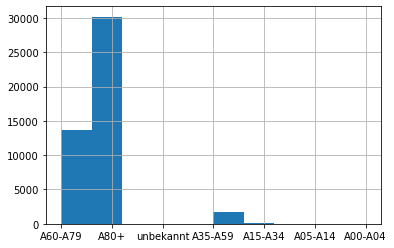
\includegraphics[scale = 0.8]{attachment/chapter_3/Scc082}
\end{figure} 
und der Todesfälle in Deutschland.
\begin{lstlisting}[style=python]
	# Filter for Infected People
	df_SKA = df_SKA.loc[lambda df: (df["AnzahlFall"]>0) & (df["AnzahlTodesfall"]>0)]
\end{lstlisting}
\begin{figure}[H]
	\centering
	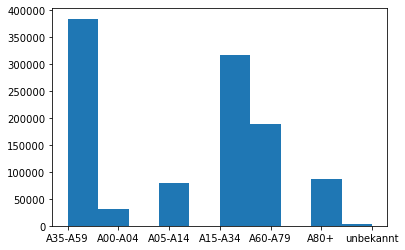
\includegraphics[scale = 0.8]{attachment/chapter_3/Scc083}
\end{figure} 
\subsubsection{Relationship Analysis}
\paragraph{Correlation, Headmap, Correlation}
\begin{itemize}
	\item seaborn df.corr()
	\item sns.headmap(df.corr())
	\item sns.pairplot(df)
\end{itemize}
Beide Funktionen corr() und sns.headmap() können nur auf metrische Variablen angewendet werden.
\begin{lstlisting}[style=python]
	import pandas as pd
	import numpy as np
	import seaborn as sns
	import datetime as dt
	
	from seaborn.palettes import color_palette
	
	# Source
	# URL: https://npgeo-corona-npgeo-de.hub.arcgis.com/datasets/dd4580c810204019a7b8eb3e0b329dd6_0
	df_SKA = pd.read_csv("RKI_COVID19.csv")
	
	#Select Data for Augsburg
	#df_SKA = df_SKA.loc[df_SKA["Landkreis"]=="SK Augsburg"]
	#	ObjectId, 
	#   IdBundesland
	#   Bundesland
	# 	Landkreis
	#   Altersgruppe
	#   Geschlecht
	#	AnzahlFall 
	# 	AnzahlTodesfall
	#	Meldedatum
	#	IdLandkreis
	#	Datenstand
	#	NeuerFall
	#	NeuerTodesfall
	#	Refdatum
	#	NeuGenesen
	#	AnzahlGenesen
	#	IstErkrankungsbeginn
	#	Altersgruppe2
	
	# Filter for Infected People
	df_SKA = df_SKA.loc[lambda df: (df["AnzahlFall"]>0) & (df["AnzahlTodesfall"]>0)]
	
	# Drops other columns
	Import_Col = [
	"Meldedatum",
	"AnzahlFall",
	"AnzahlTodesfall",
	"Altersgruppe",
	#"IdBundesland",
	"IdLandkreis",
	"Geschlecht"
	]
	df_SKA = df_SKA[Import_Col]
	
	#  Fix Date
	df_SKA["Date"] = df_SKA["Meldedatum"].apply(lambda x: dt.datetime.strptime(x, '%Y/%m/%d %H:%M:%S'))
	#df_SKA["year"] = df_SKA["Date"].apply(lambda x: x.year)
	#df_SKA["Month"] =  df_SKA["Date"].apply(lambda x: x.month)
	#df_SKA["Day"] =  df_SKA["Date"].apply(lambda x: x.day)
	df_SKA.drop(["Meldedatum"], axis=1, inplace=True)
	
	# Sort Values
	#df_SKA.sort_values(by=["Date"], inplace=True)
	
	# Relationship
	correlation = df_SKA.corr()
	sns.heatmap(correlation,xticklabels=correlation.columns, yticklabels=correlation.columns, annot=True)
	
	sns.pairplot(df_SKA)
\end{lstlisting}
\begin{figure}[H]
	\centering
	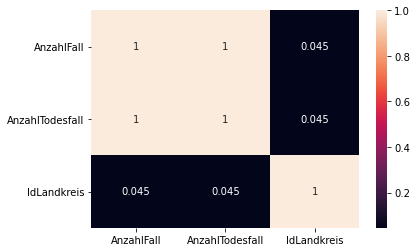
\includegraphics[scale = 0.8]{attachment/chapter_3/Scc081}
\end{figure} 

\begin{figure}[H]
	\centering
	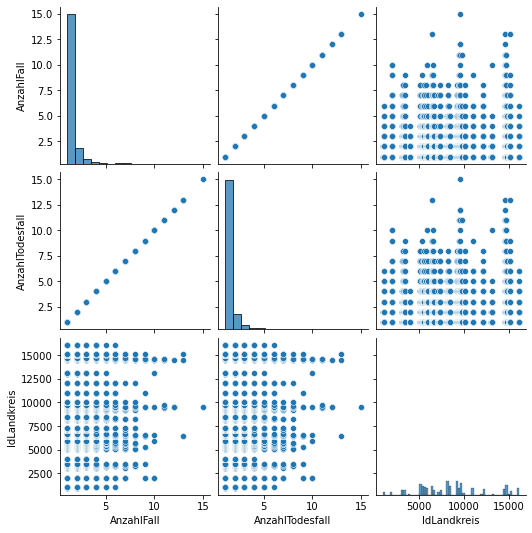
\includegraphics[scale = 0.8]{attachment/chapter_3/Scc080}
\end{figure} 
\paragraph{Relplot for Ordinal Data (Skatter Plot)}
\begin{lstlisting}[style=python]
	#%%
	import pandas as pd
	import numpy as np
	import seaborn as sns
	import datetime as dt
	
	from seaborn.palettes import color_palette
	
	# Source
	# URL: https://npgeo-corona-npgeo-de.hub.arcgis.com/datasets/dd4580c810204019a7b8eb3e0b329dd6_0
	df_SKA = pd.read_csv("RKI_COVID19.csv")
	
	#Select Data for Augsburg
	#df_SKA = df_SKA.loc[df_SKA["Landkreis"]=="SK Augsburg"]
	#	ObjectId, 
	#   IdBundesland
	#   Bundesland
	# 	Landkreis
	#   Altersgruppe
	#   Geschlecht
	#	AnzahlFall 
	# 	AnzahlTodesfall
	#	Meldedatum
	#	IdLandkreis
	#	Datenstand
	#	NeuerFall
	#	NeuerTodesfall
	#	Refdatum
	#	NeuGenesen
	#	AnzahlGenesen
	#	IstErkrankungsbeginn
	#	Altersgruppe2
	
	# Filter for Infected People
	df_SKA = df_SKA.loc[lambda df: (df["AnzahlFall"]>0) & (df["AnzahlTodesfall"]>0)]
	
	# Drops other columns
	Import_Col = [
	"Meldedatum",
	#"AnzahlFall",
	"AnzahlTodesfall",
	"Altersgruppe",
	#"IdBundesland",
	#"IdLandkreis",
	"Geschlecht"
	]
	df_SKA = df_SKA[Import_Col]
	
	#  Fix Date
	df_SKA["Date"] = df_SKA["Meldedatum"].apply(lambda x: dt.datetime.strptime(x, '%Y/%m/%d %H:%M:%S'))
	#df_SKA["year"] = df_SKA["Date"].apply(lambda x: x.year)
	#df_SKA["Month"] =  df_SKA["Date"].apply(lambda x: x.month)
	df_SKA["Day"] =  df_SKA["Date"].apply(lambda x: x.day)
	df_SKA.drop(["Meldedatum"], axis=1, inplace=True)
	
	# Sort Values
	#df_SKA.sort_values(by=["Date"], inplace=True)
	
	# Relationship
	sns.relplot(x= "Date",y="AnzahlTodesfall", hue="Geschlecht", data=df_SKA)
	# %%
\end{lstlisting}
\begin{figure}[H]
	\centering
	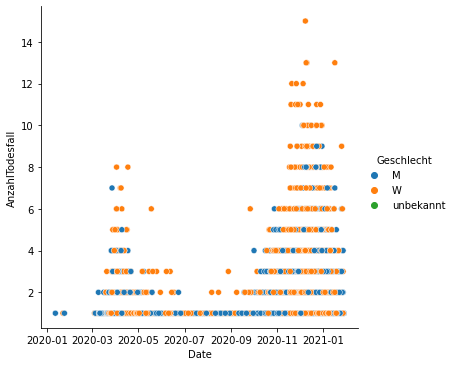
\includegraphics[scale = 0.8]{attachment/chapter_3/Scc084}
	\caption{Todesfälle}
\end{figure} 
\begin{figure}[H]
	\centering
	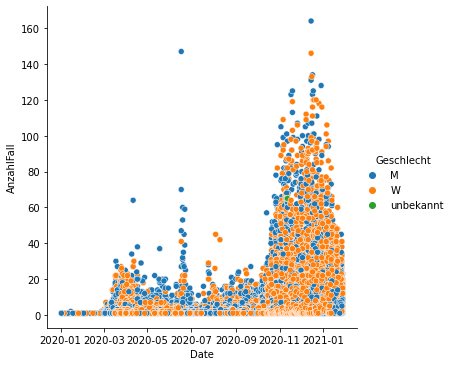
\includegraphics[scale = 0.8]{attachment/chapter_3/Scc085}
	\caption{Infektionen}
\end{figure} 
\begin{figure}[H]
	\centering
	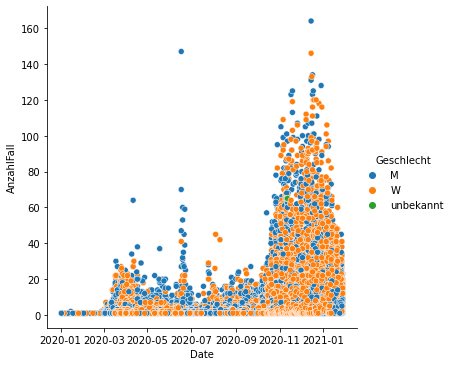
\includegraphics[scale = 0.8]{attachment/chapter_3/Scc085}
	\caption{FallAnzahl nach Altersgruppen}
\end{figure} 

\paragraph{Displot metrische Variable}
\begin{lstlisting}[style=python]
	sns.distplot(df_SKA["AnzahlFall"])
\end{lstlisting}
\begin{figure}[H]
	\centering
	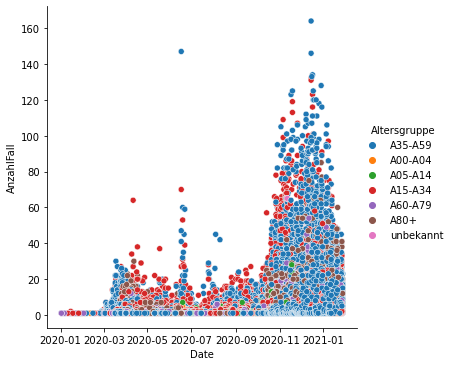
\includegraphics[scale = 0.8]{attachment/chapter_3/Scc086}
	\caption{FallAnzahl nach Altersgruppen}
\end{figure} 

Mit .replace() können die string Werte in numerische Werte überführt werden.
\begin{figure}[H]
	\centering
	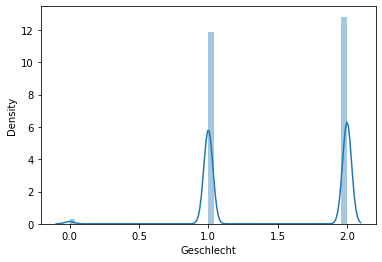
\includegraphics[scale = 0.8]{attachment/chapter_3/Scc089}
\end{figure} 

\paragraph{Boxplot}
\begin{lstlisting}[style=python]
	sns.catplot(x="AnzahlFall", kind="box", data=df_SKA)
\end{lstlisting}
\begin{figure}[H]
	\centering
	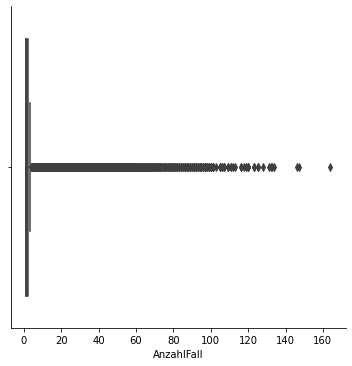
\includegraphics[scale = 0.8]{attachment/chapter_3/Scc088}
	\caption{FallAnzahl nach Altersgruppen}
\end{figure} 




\subsection{Data Visulization - Matplotlib}
\subsubsection{Preparation}
Die Daten für die Grafiken in \textit{Matplot.pyplot} bereit zu stellen, müssen einige Kriterien erfüllt sein.
\paragraph{Spalteauslesen}
Es bietet sich an, die Spalten sich als Dataframe ausgeben zu lassen. In \textit{VStudio} können diese übersichtlich angezeigt werden.
\begin{lstlisting}[style=python]
	df_i_columns = Dataframe(df_i.columns)
\end{lstlisting}
Es dürfen keine NULL Werte beinhaltet sein. Über den \textit{.info} werden die Kriterien des Dataframes ausgegeben.
\begin{lstlisting}[style=Python]
	df_i.info()
\end{lstlisting}
\begin{figure}[H]
	\centering
	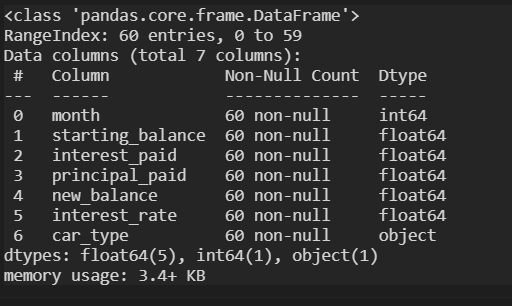
\includegraphics[scale = 0.8]{attachment/chapter_4/Scc003}
\end{figure}

\paragraph{Filter - Praxis}
Es gibt mehrere Möglichkeiten Filter bezüglich des Dataframes anzuwenden.
Eine Methode ist, Filter anzulegen und diese kombiniert über \textit{.loc} anzuwenden.
\begin{lstlisting}[style=Python]
	#%%
	# Configure Filters
	
	df_i_filter_1 = df_i[df_i_columns.iloc[8,0]] == "VW Golf R"
	df_i_filter_2 = df_i[df_i_columns.iloc[7,0]] == 0.029
	
	#%%
	# Apply one filters
	# First Methode
	df_i[df_i_filter_1]
	
	#%%
	# Apply one filters
	# First Methode
	df_filter = df_i.iloc[df_i_filter_1.array]
	df_filter.head()
	
	#%%
	# Apply two filters
	# First Methode
	df_filter_two = df_i[df_i_filter_1 & df_i_filter_2]
	df_filter_two.head()
	
	
	# %%
	# Apply two filters
	# Secound Methode
	
	df_filter_two = df_i.loc[df_i_filter_1 & df_i_filter_2]
	df_filter_two.head()
\end{lstlisting}

\paragraph{Transformation: Numpy - ndarray} 
Einzelne Spalten müssen wir die einzelne Darstellung in \textit{ndarray} umgewandelt werden. Es gibt zwei Methoden in \textit{pandas} welche dies tun. Ebenso gibt es Methoden, welche nur Arrays ausgeben, dies aber nicht in \textit{ndarrays} transformieren.
\begin{itemize}
	\item \textit{df.values} oder 
	\item \textit{df.to$\_$numpy()}
\end{itemize}
\begin{lstlisting}[style=Python]
	# %%
	### Preparation for mathplot
	
	# ndarray (numpy) Month
	varSelCol_3 = df_i_columns.iloc[0,0]
	nda_Month = df_i[varSelCol_3].values
	
	# ndarray (numpy) Interest Paid
	varSelCol_3 = df_i_columns.iloc[[0,1,2],0]
	nda_interest_paid = df_i[varSelCol_3].values
	
	# ndarray (numpy) Prinzipal Paid
	varSelCol_3 = df_i_columns.iloc[3,0]
	nda_prinzipal_paid = df_i[varSelCol_3].to_numpy()
\end{lstlisting}
\begin{figure}[H]
	\centering
	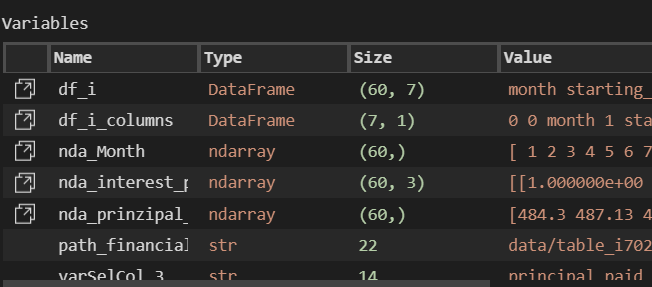
\includegraphics[scale = 0.8]{attachment/chapter_4/Scc004}
\end{figure}
Die letzte Funktion wird von \textit{pandas} vorgeschlagen, als die zu bevorzugenden Funktion. \\

Die Auslesung einer Spalte reicht nicht aus. Hierbei wird nur eine \textit{Series} zurückgegeben.

)
\paragraph{Historischer Abriss}
Um fehlende Werte in Python zu verstehen, muss die historisch, gewachsenen Struktur der Pakete \textit{pandas}, \textit{NumPy}, sowie der Sprache \gls{R} betrachtet werden.\\

\begin{itemize}
	\item Die Begriffe \gls{g_None} und \gls{g_NULL} sind inhaltlich gleich. In Python wird nur \gls{g_None} verwendet. Als Beispiel in \gls{CPP} und Power BI wird \gls{g_NULL} verwendet.
	\item In Python selbst gibt es viele Pakete (\textit{NumPy}, \textit{Math}) welche \gls{g_NaN} ermöglichen: $np.nan$.
	\item Die Pakete \textit{pandas} und \textit{NumPy} sind in Anlehnung an \gls{R} geschrieben worden.
	\item Die Begrifflichkeit \gls{Na} gibt in Python nicht, sondern wurde nur aus historischen Gründen übernommen.
	\item \textit{Pandas} ist aufbauend auf \textit{NumPy} geschrieben worden. Es unterscheidet jedoch nicht mehr zwischen NaN aus \textit{NumPy} und \gls{g_None}. Die Funktionen 
	\begin{align}
		Dataframe.isnull()\\
		Dataframe.isna()
	\end{align}
	geben das gleich aus.
\end{itemize}

\paragraph{Umgang in Pandas mit NaN}
\textit{Pandas} unterscheidet bei der Suche nach fehlenden Daten nicht zwischen den beiden Datentypen \gls{g_None} und \gls{NaN}. Die Funktionen
\begin{align}
	pandas.isnull()
\end{align}
und 
\begin{align}
	pandas.isna()
\end{align}
geben die gleichen \textit{Wahr}/\textit{Falsch} Werte zurück. Dies gilt ebenso bei der Anwendung auf Dataframes 
\begin{lstlisting}[style=Python]
	df = pd.DataFrame([2,np.nan, None])
	df["2"] = df[0].isnull()
	df["3"] = df[0].isna()
	df
\end{lstlisting}
\begin{figure}[H]
	\centering
	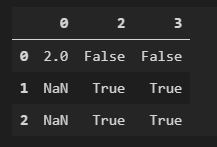
\includegraphics[scale = 0.8]{attachment/chapter_4/Scc008}
\end{figure}
Hinzu kommt, dass Pandas \gls{g_None} in \gls{NaN} in \gls{NaN} umwandelt. Die Funktion \textit{isnull()} und \textit{isna()} ist auf das Fundament in \gls{R} zurück zuführen.\\

Die Werte in Variablen abgespeichert, erzielen das gleiche Resulat, bei einer Gleichheitsabfrage:
\begin{lstlisting}[style=Python]
	x = np.nan
	y = np.nan
	x == y # False
\end{lstlisting}
Wir gefragt, ob es sich um das gleiche Objekt \bl{is} handelt, wird bei den Variablen 
\begin{lstlisting}[style=Python]
	x is y # True
\end{lstlisting}
dies bejaht. \\

Befindet sich \textit{NaN} in einem Dataframe, wird \textit{false} zurückgegeben:
\begin{lstlisting}[style=Python]
	df = pd.DataFrame([None,np.nan, 3], [4, None, None])
	df["5"] = df[0] == np.nan
	df["6"] = df[0] is np.nan
	df
\end{lstlisting}

\begin{figure}[H]
	\centering
	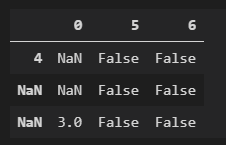
\includegraphics[scale = 0.8]{attachment/chapter_4/Scc009}
\end{figure}
Der Grund ist, dass im Dataframe \gls{g_NaN} anders codiert ist. Für weiteres siehe das Glossar: \gls{g_NaN}.

\paragraph{Umgang mit None}
Der Wert \gls{g_None} ist immer der selbe, weshalb die Gleichheitsabfrage \textit{true} zurückgibt. Ebenso ist die Identität eines jeden \gls{g_None} Wertes auf ein Objekt zurückzuführen: TypNone
\begin{lstlisting}[style=Python]
	x = None
	y = None
	x == y # True
	x is y # True
\end{lstlisting}

\paragraph{Näheres zu None und NULL}
In Python existiert das Konzept \gls{g_None}, welches aus die Funktion von \gls{g_NULL} aus anderen Sprachen übernimmt. Die Funktion \textit{print()} ist Funktion, welche \gls{g_None} wieder gibt. 
\begin{lstlisting}[style=Python]
	print("Hello")
	>>> Hello
	print(print("Hello"))
	>>> Hello
	>>> None
\end{lstlisting}

\footnote{
	\href{https://www.r-bloggers.com/2010/04/r-na-vs-null/}{Unterschied in R zwischen NaN und NULL}, \href{https://datascience.stackexchange.com/questions/37878/difference-between-isna-and-isnull-in-pandas}{Unterschied zwischen den Funktionen in Pandas und NumPy}, 
	\href{https://www.r-bloggers.com/2010/04/r-na-vs-null/}{r-na-vs-null},
	\href{https://realpython.com/null-in-python/}{Null in Python}
}

\paragraph{Removing or filling in missing data}
\paragraph{.dropna()}
\begin{lstlisting}[style=Python]
	
	### Loading Data
	#path_financial = "data/car_financing.csv"
	path_financial = "data/table_i702t60.csv"
	df = pd.read_csv(path_financial)
	
	# %% Scaning Data
	df.info()
	# %% Adding a missing value
	df.iloc[2,2] = np.nan
	# %% Check up
	df.info()
	# %% Droping rows
	'''
	The function .dropna() allows to delete any rows, with np.nan values.
	axis:[0,1], default 0
	how : ['any,all'], default 'any'
	- 'any': If any nan are present drop the row or column
	- 'all': If all values are nan, drop row or column
	etc.
	'''
	df.dropna(how='any', inplace = True)
\end{lstlisting} 
\paragraph{Fill-In: General} Im allgemeinen ist \textit{.iloc()} nicht dafür ausgelegt, dass diese Funktion Werte im ursprünglichen Dataframe anpassen. Es kann verwendet werden, wie zum Beispiel:
\begin{lstlisting}[style=Python]
	#%% Replace Values
	for i in range(3,6):
	df.iloc[i,2]= 3
\end{lstlisting}
\begin{figure}[H]
	\centering
	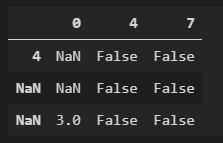
\includegraphics[scale = 0.8]{attachment/chapter_4/Scc010}
\end{figure}
Gleich ist es möglich mit der dopple Indexierung die Werte zu ändern:
\begin{lstlisting}[style=Python]
	# %% For loop Changing Value
	for i, j in enumerate(df_column):
	df.loc[i,j] = np.nan
\end{lstlisting}
Achtung, wenn Zeilen fehlen, oder durch vorherige Schritte entfernt werden, sind die Indexies nicht mehr vorhanden, und können zu Problemen führen:
\paragraph{Fill-In: fillna()} Der entsprechende Bereich kann ersetzt werden.
\begin{lstlisting}[style=Python]
	'''
	DataFrame.fillna(value=None, method=None, axis=None, inplace=False, limit=None, downcast=None)[source]
	Fill NA/NaN values using the specified method.
	
	Parameters
	valuescalar, dict, Series, or DataFrame
	Value to use to fill holes (e.g. 0), alternately a dict/Series/DataFrame of values specifying which value to use for each index (for a Series) or column (for a DataFrame). Values not in the dict/Series/DataFrame will not be filled. This value cannot be a list.
	
	method{‘backfill’, ‘bfill’, ‘pad’, ‘ffill’, None}, default None
	Method to use for filling holes in reindexed Series pad / ffill: propagate last valid observation forward to next valid backfill / bfill: use next valid observation to fill gap.
	
	axis{0 or ‘index’, 1 or ‘columns’}
	Axis along which to fill missing values.
	
	inplacebool, default False
	If True, fill in-place. Note: this will modify any other views on this object (e.g., a no-copy slice for a column in a DataFrame).
	
	limitint, default None
	If method is specified, this is the maximum number of consecutive NaN values to forward/backward fill. In other words, if there is a gap with more than this number of consecutive NaNs, it will only be partially filled. If method is not specified, this is the maximum number of entries along the entire axis where NaNs will be filled. Must be greater than 0 if not None.
	
	downcastdict, default is None
	A dict of item->dtype of what to downcast if possible, or the string ‘infer’ which will try to downcast to an appropriate equal type (e.g. float64 to int64 if possible).
	
	Returns
	DataFrame or None
	Object with missing values filled or None if inplace=True.
	'''
\end{lstlisting}
Die Funktion \textit{.fillna()} ermöglicht es \gls{NaN} Wert direkt zu ersetzten.
\begin{figure}[H]
	\centering
	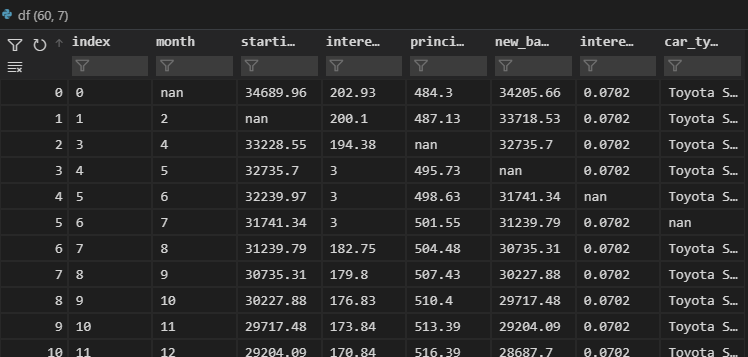
\includegraphics[scale = 0.8]{attachment/chapter_4/Scc012}
\end{figure}
\begin{lstlisting}[style=Python]
	df.info()
\end{lstlisting}
\begin{figure}[H]
	\centering
	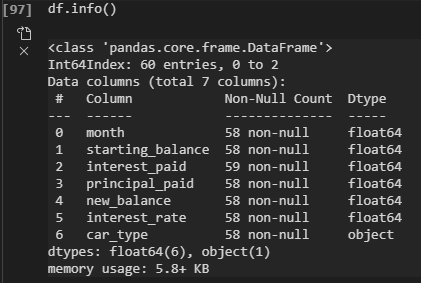
\includegraphics[scale = 0.8]{attachment/chapter_4/Scc013}
\end{figure}
\begin{lstlisting}[style=Python]
	df.fillna("x", inplace = True)
\end{lstlisting}
\begin{lstlisting}[style=Python]
	df.info()
\end{lstlisting}
\begin{figure}[H]
	\centering
	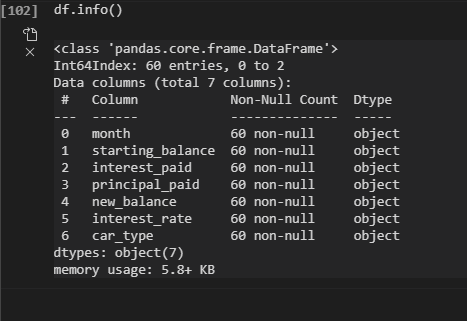
\includegraphics[scale = 0.8]{attachment/chapter_4/Scc014}
\end{figure}

\paragraph{Fill in directly}
\begin{lstlisting}[style=Python]
	varIsNull = df["interest_paid"].isna()
	df["interest_paid"].iloc[varIsNull] = "y"
\end{lstlisting}

\paragraph{Converting Dataframe to NumPy}\label{Converting Dataframe to NumP}

\begin{lstlisting}[style=Python]
	df.to_numpy() # NumPy Array
	df.values # NumPy Array
	df.to_dict() # Dictionaries
\end{lstlisting}
\subsubsection{Simple Plot}
Die Funktion \textit{plt.plot()} benötigt als Inputs \textbf{NumPy Arrays}. Liegt Datensätze in Form eines pandas Dataframe vor, so müssen die einzelnen Spalten in solche konvertiert werden, siehe \ref{Converting Dataframe to NumP}.

\begin{lstlisting}[style=Python]
	#%% Import Packages & Data
	
	import pandas as pd
	import numpy as np
	import matplotlib.pyplot as plt 
	import seaborn as sns 
	
	
	'''Loading Data'''
	path_financial = "data/car_financing.csv"
	#path_financial = "data/table_i702t60.csv"
	df_i = pd.read_csv(path_financial)
	
	''' Extract column names'''
	df_i_columns = pd.DataFrame(df_i.columns)
	
	#%% Check for NaN or Null Values
	df_i["car_type"].unique()
	
	# %% Filter with iloc
	filter_cartype = df_i["car_type"] == "Toyota Corolla"
	df_i = df_i.iloc[filter_cartype.array]
	
	
	# %% Preparation for mathplot
	
	'''Month'''
	varSelCol_3 = df_i_columns.iloc[0,0]
	nda_Month = df_i[varSelCol_3].to_numpy()
	
	''' Interest Paid'''
	varSelCol_3 = df_i_columns.iloc[3,0]
	nda_interest_paid = df_i[varSelCol_3].values
	
	'''Prinzipal Paid'''
	varSelCol_3 = df_i_columns.iloc[4,0]
	nda_prinzipal_paid = df_i[varSelCol_3].to_numpy()
\end{lstlisting}
Ist dies geschehen, kann mit \textit{plt.plot()} ein Graf erzeugt werden.

\begin{lstlisting}[style=Python]
	plt.plot(nda_Month,nda_interest_paid)
\end{lstlisting}

\begin{figure}[H]
	\centering
	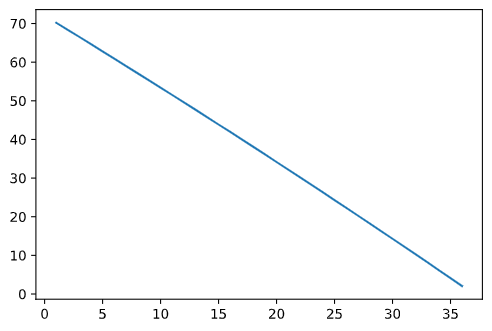
\includegraphics[scale = 0.8]{attachment/chapter_4/Scc015}
\end{figure}

Wird zwei \textit{plt.plot()} erstellt, werden diese in einer Grafik zusammengefügt
\begin{lstlisting}[style=Python]
	# %% Plot two graphs in one grahic
	plt.plot(nda_Month, nda_prinzipal_paid)
	plt.plot(nda_Month, nda_interest_paid)
\end{lstlisting}
\begin{figure}[H]
	\centering
	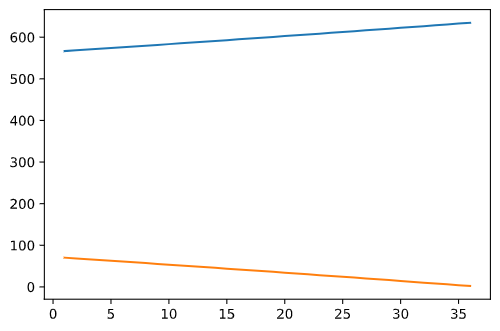
\includegraphics[scale = 0.8]{attachment/chapter_4/Scc016}
\end{figure}
\paragraph{Styles}
Mit \textit{plt.style.available} werden die verschiedensten Styles in Matplot angezeigt. Unter Einbindung von seaborn stehen mehr Styles zur Verfügung.
\begin{lstlisting}[style=Python]
	# %% Chosoe Style
	plt.style.available
\end{lstlisting}
\begin{figure}[H]
	\centering
	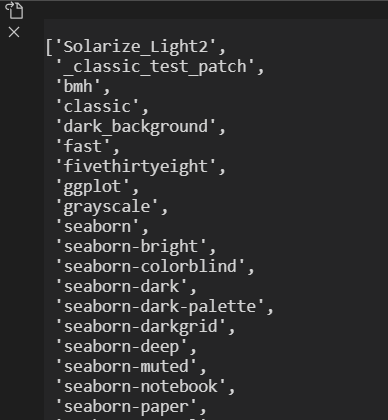
\includegraphics[scale = 0.8]{attachment/chapter_4/Scc017}
\end{figure}
Den Style zu ändern, erfolgt über \textit{plt.style.use()}.
\begin{lstlisting}[style=Python]
	# %% Choose Style
	plt.style.use("seaborn-dark")
	plt.plot(nda_Month, nda_prinzipal_paid)
\end{lstlisting}

\paragraph{Marker Type and Colors}
\begin{itemize}
	\item maker - Einzelne Datenpunkte
	\item markersize - Größe von Marker
	\item c - Colour Template
\end{itemize}
\begin{lstlisting}[style=Python]
	# %% Marker and Colour
	Grafik_1 = plt.plot(nda_Month, nda_prinzipal_paid, marker = ".", markersize = 10, c = "k")
	Grafik_2 = plt.plot(nda_Month, nda_interest_paid, marker = ".", markersize = 8, c = "k")
\end{lstlisting}
\begin{figure}[H]
	\centering
	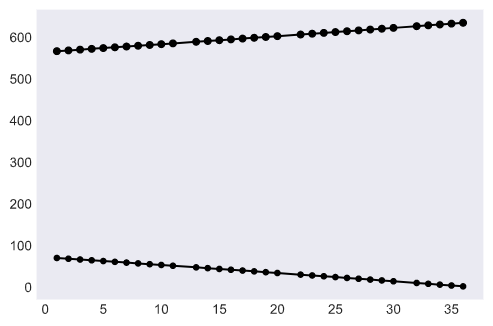
\includegraphics[scale = 0.8]{attachment/chapter_4/Scc018}
\end{figure}




\subsubsection{MATLAB-Style vs Object-Oriented Style}
\paragraph{Subplots - Two simple Figures}
Über Matplotlib können zwei verschiedene Syntaxen verwendet werden:
\begin{itemize}
	\item \textbf{MATLAB} Style und oder
	\item \textbf{Objektorientierte} Syntax. \footnote{\cite{URL.Python-Tutorial}, \cite{}Book.Python-DSci}
\end{itemize}

Die Syntax wurde von MATLAB übernommen, weshalb es viele Gleichheiten mit der Python Alternative, Matplotlib, gibt.\\

\paragraph{Matlab}
Im ersten Beispiel wird dargestellt, wie in dem \textit{MATLAB-Style} Grafiken mit Hilfe von \textit{plt.subplot()} dargestellt werden.\footnote{Wird \textit{plt.subplot() ohne Argument erstellt, so wird eine Objekt mit einer Zeile und einer Spalte erstellt.}}
\begin{itemize}
	\item Die Parameter \textit{nrows}, \textit{ncols} und \textit{index} der Funktion \textit{subplot()} geben an, wie viele Panele erstellt werden.
	\item Dabei wird für jeden Subplot die gleich Konfiguration benötigt. Der \textit{index} gibt dabei an, in welchem Panal der Plot angefügt werden soll.
	\item Wird \textit{plt.figure} nicht angegeben, wird bei dieses \textit{plt.subplot} impliziert erstellt
\end{itemize}

\begin{lstlisting}[style=Python]
	#%% Import Packages
	import pandas as pd
	import numpy as np
	import matplotlib.pyplot as plt 
	import seaborn as sns 
	
	#%% Creating Variables
	x = np.linspace(0,50,1000)
	
	#%% Create a plot figure
	plt.figure() # create a figure object
	
	plt.subplot(2,2,1) # row, column, panel
	plt.plot(x, np.sin(x))
	
	plt.subplot(2,2,4)
	plt.plot(x, np.cos(x))
	
	plt.subplot(2,2,2)
	plt.plot(x, np.sin(x)+2)
	
	plt.subplot(2,2,3)
	plt.plot(x, np.sin(x)*3)
	
	plt.title("Hello") # Title for the figure
\end{lstlisting} \footnote{\cite[240]{Book.Python-DSci}}





Der Nachteil dieses Styles ist es, dass es aufwendig ist, neue Panale hinzuzufügen. Es müssen alle Konfigurationen angepasst werden.\\
\begin{figure}[H]
	\centering
	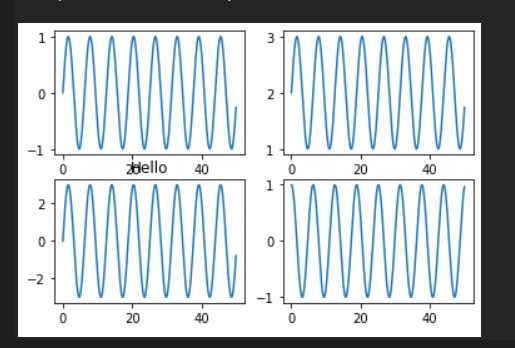
\includegraphics[scale = 0.8]{attachment/chapter_4/Scc019}
\end{figure}
\paragraph{OO}
In dem objekt-orientierenden Style wird eine Figure Objekt erstellt und die Panele in dem Objekt \textbf{ax} gespeichert. Die Anzahl der Panele bestimmt die Anzahl der geplotteten Grafiken. \\

\textbf{ACHTUNG:} Die Funktion heißt plt.subplot\textcolor{red}{s} nicht plt.subplot.

\begin{lstlisting}[style=Python]
	fig, ax = plt.subplots(2)
	
	ax[0].plot(x, np.sin(x))
	ax[1].plot(x, np.sin(-x))
\end{lstlisting}
\begin{figure}[H]
	\centering
	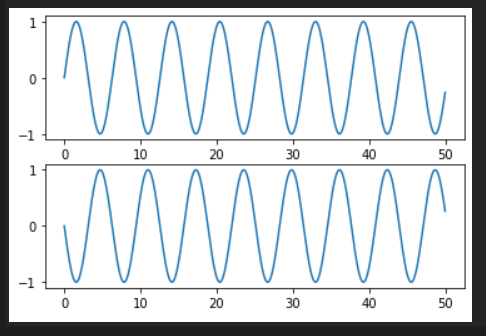
\includegraphics[scale = 0.8]{attachment/chapter_4/Scc020}
\end{figure}

\paragraph{Simple Linie Plot}
Die Instanzen der Objekte Figure und Axes sehen wie folgt leer aus.
\begin{lstlisting}[style=Python]
	# %% Seaboarn Style
	plt.style.use('seaborn-whitegrid')
	
	figure_l = plt.figure() # Create instance of the object figure
	axis_l = plt.axes() # Create instance of the object axes
\end{lstlisting}
\begin{figure}[H]
	\centering
	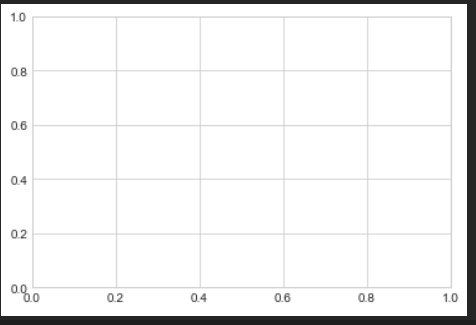
\includegraphics[scale = 0.8]{attachment/chapter_4/Scc021}
\end{figure}
Dabei produziert der Befehlt ohne \textit{plt.figure} eine Grafik, hingegen anders herum nicht.

Die Instanz \textit{Figure} kann so verstanden werden, dass es alle Instanzen von \textit{axis}, \textit{label}, \textit{title} und \textit{graphics} umschließt.

Im Folgenden soll die Funktion $f(x)=\sin(x)$ mit $x\in [0,10]$ in den zwei Formen abgebildet werden. Im objekt-orientierten Style wird dies über die Objekte Axis und Figure dargestellt:
\begin{lstlisting}[style=python]
	# %% Seaboarn Style
	plt.style.use('seaborn-whitegrid')
	
	x_sin = np.linspace(0,5,num=1000) # Generate Input
	
	figure_l = plt.figure() # Create instance of the object figure
	axis_l = plt.axes() # Create instance of the object axes
	
	axis_l.plot(x, np.sin(x))
\end{lstlisting}
Ohne dies kann es über 
\begin{lstlisting}[style=python]
	plt.plot(x,np.sin(x))
\end{lstlisting}
angesteuert werden.

\paragraph{Same Function in Both Styles}
Der Prefix lautet \textit{plt.} oder \textit{ax.}
\begin{itemize}
	\item legend()
	\item plot()
	\item etc.
\end{itemize}

\paragraph{Different Function in Both Styles}
Es gibt Funktionen, die den gleichen Inhalt vermitteln, aber unterschiedlich Syntax besitzen.
\begin{itemize}
	\item Achsen Grenze bestimmen:
	\begin{lstlisting}[style=python]
		# M
		plt.plot()
		plt.xlim()
		# OO
		ax.plot()
		ax.set_xlim()
	\end{lstlisting}
	\item Achsen Titel bestimmen:
	\begin{lstlisting}[style=python]
		# M
		plt.plot()
		plt.xlabel()
		# OO
		ax.plot()
		ax.set_xlabel())
	\end{lstlisting}
	\item Grafik Titel bestimmen:
	\begin{lstlisting}[style=python]
		# M
		plt.plot()
		plt.titel()
		# OO
		ax.plot()
		ax.set_title())
	\end{lstlisting}
\end{itemize}
Der Vorteil gegenüber de Matlab-Notierung ist, dass über die \textit{.set()} Funktion die einzelnen Bestanteile gemeinsam aufgerufen werden können.
\begin{lstlisting}[style=python]
	
	# %% Seaboarn Style
	plt.style.use('seaborn-whitegrid')
	
	x_sin = np.linspace(0,5,num=1000) # Generate Input
	
	figure_l = plt.figure() # Create instance of the object figure
	axis_l = plt.axes() # Create instance of the object axes
	
	axis_l.plot(x, np.sin(x))
	
	axis_l.set(xlim=(0,10), ylim=(-1,1), title="Cool")
\end{lstlisting}

\begin{figure}[H]
	\centering
	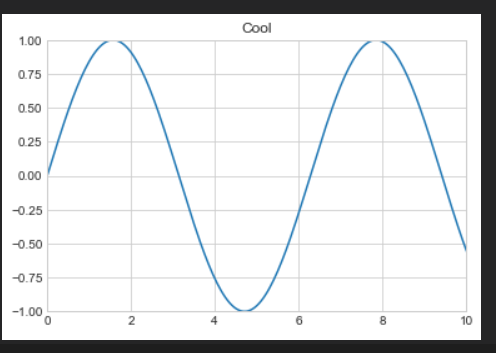
\includegraphics[scale = 0.8]{attachment/chapter_4/Scc022}
\end{figure}

 % Libraries for Data Analysis (Pandas, Matplotlib, etc.)

%\pagebreak
\chapter{ML with SciKit-Learn}
\setcounter{section}{0}
 % ML SciKit-Learn 
%\section{Scikit Learn 3 h}
\subsection{Overview}
Im ersten Teil von Scikit Learn wir darauf eingegangen, dass ML-Algorithmen zwar in einer fülle leicht verfügbar ist, aber in der praktischen Anwendung schwerer auszuwählen und implementieren ist.
\subsection{Pre Processing}
Die Aussagekraft eines Model ist von der Qualität der Input Daten abhängig. Die Vorbehandlung der Daten ist von großer Bestandteil der Modellierung.

\subsection{Metrics}
Um die ersten beiden Punkt auf Valität zu überprüfen, ist Ziel dieses Kapitels. Scikit Learn bietet eigene Metriken an, um zu Qualtiät eines Modells zu bestimmen. Ebenso wird hier gezeigt, wie eigene Metriken genutzt werden können.

\subsection{Meta Esitmator}
*Nachdem das Modell einen PreProcessing Schritt und eine Vorhersage getroffen hat, kann ein Meta Estimator gefunden werden
% Unklar, was damit gemeint ist.
 % Scikit-Learn 3 hours
%\section{Data Preprocessing: Categorial Values}
%Quelle: Working with Predictive Analytics} 
In diesem Themen-Block wurden die Kategorischen Varialben aufgegriffen, und die Option des One Hot und Label Encoders.

Prozesse und Algorithmen im \gls{ML} Bereich benötigen als Input numerische Werte. Daten diese dies nicht bieten können, müssen in solche kodiert werden.

Es gibt dafür zwei bestehende Methoden im sklearn Paket:
\begin{itemize}
	\item 
	\begin{lstlisting}[style=python]
		from sklearn import preprocessing
		le = preprocessing.LabelEncoder()	 # Create a class object
	\end{lstlisting}
	\item 
	\begin{lstlisting}[style=python]
		
	\end{lstlisting}
\end{itemize}

\paragraph{Label Encoder}
Der Preprocessor von \gls{g_scikit} bietet eine Classe an, welche Kategorische Werte eines Arrays in numerische umwandelt.
Dies ist notwendig, weil ML-Modelle nur numerische Werte einlesen.
Haben die Werte eine ordinale Struktur, kann ein ML Modell diese abbilden. Ist dies jedoch nicht vorhanden, so bietet One Hot Encoder eine bessere Struktur an.

\begin{lstlisting}[style=python]
	#################### Python Libraries
	import pandas as pd
	import numpy as np
	from sklearn.model_selection import train_test_split
	from sklearn.impute import SimpleImputer
	import matplotlib.pyplot as plt
	
	# Label Encoder
	from sklearn.preprocessing import OneHotEncoder
	from sklearn.preprocessing import LabelEncoder
	from sklearn.compose import ColumnTransformer
	
	#################### Import Date
	data = pd.read_csv("insurance.csv")
	
	#################### EDA
	
	#print(data.head(3))
	#print(data.describe())
	#print(data["bmi"].unique())
	#data_nan = data.isnull().sum()
	#print(data_nan)
	
	#################### Data Prepartion
	
	data["bmi"].fillna(0, inplace = True) # replace None
	#print(data.head(3))
	data_mod = data
	
	#################### Label Encoding
	LE = LabelEncoder()
	data_mod["sex"] = LE.fit_transform(data["sex"]) # input is an array
	data_mod["region"] = LE.fit_transform(data["region"])
	data_mod["smoker"] = LE.fit_transform(data["smoker"])
	print(data_mod.iloc[:,1:].head())	
\end{lstlisting}

Im Klassenobjekt werden die Kategorien wie weitere Funktion zum Input Array gespeichert. Wir das Klassenobjekt auf eine anderes Array angesetzt, so werden die vorherigen Daten überschrieben.
\begin{lstlisting}[style=python]
	LE = LabelEncoder()
	data_mod["sex"] = LE.fit_transform(data["sex"]) # input is an array
	data_mod["region"] = LE.fit_transform(data["region"])
	data_mod["smoker"] = LE.fit_transform(data["smoker"])
	print(data_mod.iloc[:,1:].head())
	
	# Inverse encoder
	print(LE.classes_)
	#data_mod["New"] = LE.inverse_transform(data_mod["region"] #Fuehrt zum Fehler
	data_mod["New"] = LE.inverse_transform(data_mod["smoker"]
\end{lstlisting}

\paragraph{One Hot Encoder}
Um eine Ordnung in den transformierten Daten zu vermeiden, wenn keine existiert, werden Dummy Variablen angelegt. \\

Im ersten Schritt wird der Konstruktor geschaffen, dann die jeweiligen Operationen durchgeführt.
\begin{lstlisting}[style=python]
	O_OHE = OneHotEncoder(categorial_feature=[0])
	O_OHE.fit_Transform1	
\end{lstlisting}
Das label-encodedet Array wird aufsplittet in die Anzahl Spalten wie das Array eindeutige Kategorien hat.
 %  Encoder Categorial Values
%\section{Clustering: K-Means}
% Genaue Betrachtung des K-Means wurde gestartet, die Beispiele müssen herauskommen, und in Beispiel Skripte überführt werden.

\subsection{Introduction}
\begin{itemize}
	\item Die Grundidee ist, einen Datensatz in $k$ Partitionen zu teilen, sodass die Summe der quadrierten Abweichungen von den Cluster-Schwerpunkten minimal ist.
	\begin{align}
		J = \sum_{i=1}^{k}\sum_{x_j\in S_i} \left| \left| x_j - \mu_i \right| \right|^2  
	\end{align}
	mit den Datenpunkten $x_j$ und den Schwerpunkten $\mu_i$ der Cluster $S_i$.
	\item Man spricht von \textit{Clustering durch Varianzminimierung}.
	\item Der Ausdruck $\left| \left| x_i -\mu_i \right| \right|^2$ beschreibt die Euklidische Distanz zwischen dem Datenpunkt und dem Schwerpunkt $\mu_i$ des jeweiligen Clusters $S_i$.
	\item Zum Anfang werden $k$ Cluster ausgewählt.
	\item Das Ziel ist, dass jedes Objekt am Ende einem Clusterschwerpunkt zugewiesen wird.
	\item Schwachstellen des Algorithmus ist, dass die mehrere Lösungen gefunden werden können. Diese hängen von der Wahl der Startpunkt für $\mu_i$ ab. \\
	
	Es gibt verschiedene Algorithmen die die Möglichkeit anbieten, mehrere Iterationen durchzuführen, mit verschiedenen Startwerten.
	\item Eine weitere Schwachstelle ist, dass die Anzahl von $k$ am Anfang festgelegt werden muss. Welches $k$ das richtig ist, kann somit nach den jeweiligen Iterationen passieren.
	\item Für beide Schwachstellen hilft der \textit{Silhouttenkoeffizient}.
	\item Der Algorithmus sucht stets nach konvexen Clustern. Andere Algorithmen können auch andere anders geformte, dichtebasisierte Cluster finden, z. B. \textit{DBSCAN}.
	\item Weil der Algorithmus jeden Punkt einem Cluster zuweist, können Außreißer das Ergebnis verfälschen. Eine \textit{Noisereduction} ist vorher durchzuführen oder andere Algorithem auszuwählen.
\end{itemize}

\subsection{Silhoutte}
Eine Silhoutten gibt Auskunft, wie gut die Zuordnung einer Beobachtung $o$ zu den nächstgelegenen Clustern $A$ und $B$.\\

Darauf aufbauend ist der \textit{Silhouttenkoeffizent}. Dies ist eine Maßzahl für die Qualität der Cluster unabhängig deren Anzahl.

\paragraph{Silhoutte}
Gehört $o$ zum Cluster $A$, so ist die \textit{Silhoutte} von $o$ definiert als: 
\begin{align}
	S(o)= \begin{cases}
		0 & \text{, wenn $o$ einziges Element von $A$ ist} \\
		\dfrac{dist(B,o) - dist(A,0)}{\max\left\lbrace dist(B,o),dist(A,o)\right\rbrace} & \text{, sonst}
	\end{cases}
\end{align}

Die Distanz zwischen dem Objekt $o$ und dem Cluster $A$ sowie $B$ wird durch die maximale Distanz. Daraus folgt, dass $S(o)$ zwischen $-1$ und $1$ liegt.

\begin{itemize}
	\item $S(o) < 0$, dann gehört das Objekt zum nächstgelegenen Cluster $B$. - Das Cluster kann verbessert werden oder Außreißer entfernt.
	\item $S(o) \approx 0$, dann liegt das Objekt zwischen beiden Clustern.
	\item $S(o) \approx 1$, dann liegt das Objekt im richtigen Cluster.
\end{itemize}

Die Berechnung der Distanz zwischen dem Objekt $o$ und dem Cluster $A$ erfolgt wie:
\begin{align}
	dist(A,o) = \frac{1}{n_A - 1}\sum_{a\in A, a \neq o} dist(a,o)
\end{align}
als der Mittelwert der Distanz zwischen \textit{allen anderen Objekten} im Cluster $A$ und dem Objekt $o$. Die Anzahl der Objekte im Cluster $A$ wird mit $n_A$ definiert.\\

Analog wird die Distanz zum nächstgelegenen Cluster $B$ berechnet als die minimale durchschnittliche Distanz
\begin{align}
	dist(B,o) = \min_{C\neq A} \underbrace{\left(\frac{1}{n_c} \sum_{c\in C}dis(C,o)\right)}_{=dist(C,o)}
\end{align}
Dabei wird für alle Cluster, die das Objekt $o$ nicht enthalten\footnote{Weil $o$ in $A$ liegt.} die Distanz $dist(C,o)$ berechnet. Der nächstgelegene Cluster ist der mit der kleinsten Distanz.

\paragraph{Silhouettenkoeffizient}
Der Silhouttenkoeffizient ist definiert als 
\begin{align}
	s_C = \frac{1}{n_C}\sum_{o\in C}S(o)
\end{align}
arithmetisches Mittle aller $n_C$ Silhoutten eines Clusters $C$.
Diese Koeffizient kann für jeden Cluster oder den gesamten Datensatz berechnet werden.

\subsection{Test Data Sets}
Neue Algorithmen können problemlos arbeiten, diese zu testen, ob sie das tun, was sie tun sollen, ist nicht immer erkennbar. \\

Dafür hat \textit{scikit} Datensatz Pakete. Diese ermöglichen spezifischen Datensätze zu generieren, die 
\begin{itemize}
	\item in ihren Hyperparameter angepasst werden
	\item und skalierbar sind.
\end{itemize}

Im folgenden sollen drei Problem von \textit{Klassifikation} aufgegriffen. Dabei beschreibt \textit{Klassifikation}, dass einem Teilmengen eines Datensatzes \textit{Labels} zu gewissen werden. 

\begin{figure}[H]
	\centering
	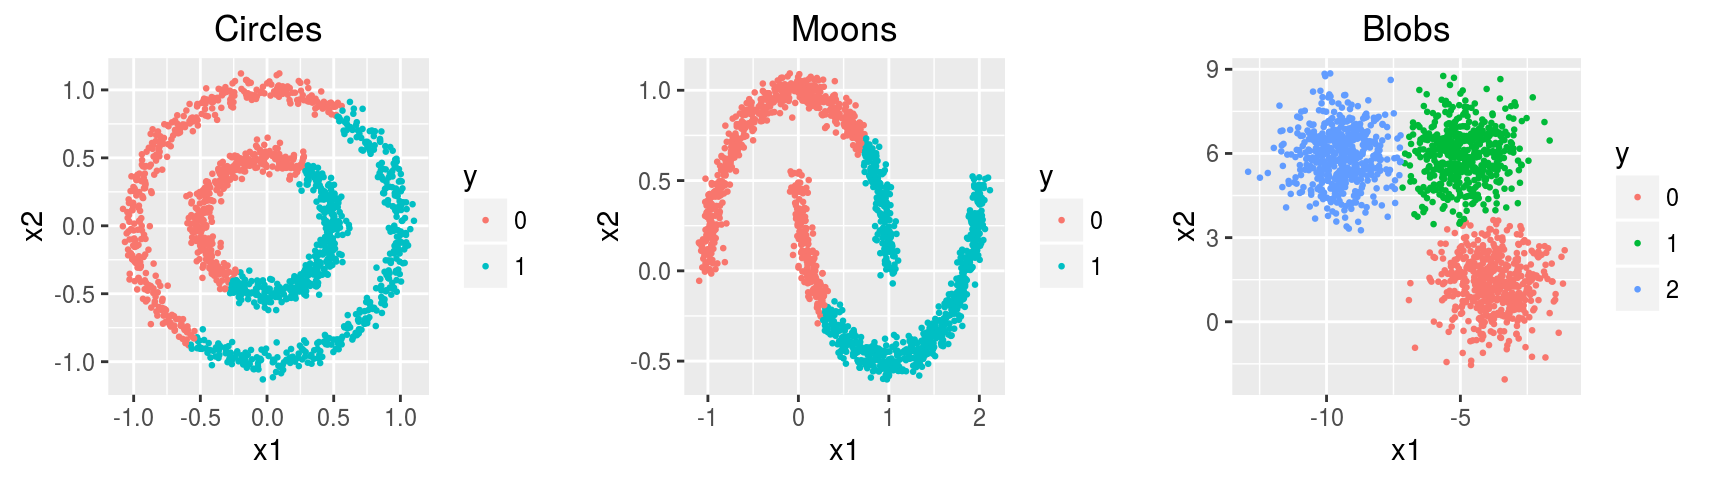
\includegraphics[scale = 0.8]{attachment/chapter_1/Scc160}
	\caption{Blobs, Moons, Circles}
\end{figure} 


\subsection{Blobs Classification Problem}
Die Funktion $make\_ blobs()$ generiert einen Datensatz, welcher $n$ Cluster beinhaltet. Dabei werden die Cluster zufällig gesetzt und die Datenpunkte um die Zentren normalverteilt. Die unabhängigen Dimensionen, oder auch \textit{Features} genannt, können ebenso bestimmt werden. Eine Visualisierung von zwei bis drei Features ist nur möglich. Die Labels werden ebenfalls als zweiter Output mit ausgegeben.
\begin{lstlisting}[style=Python]
	# Generate classification dataset
	X, labels = make_blobs(
	n_samples=100, #n-datapoints equalie devided amoung the centers
	centers=2, #centers in the dataset
	n_features=2 #columns return
	)
\end{lstlisting}

Im Folgenden wird eine Größe der \textit{Features} höher 2 nicht betrachtet, weil der Plot auf 2D ausgelegt ist.
\begin{figure}[H]
	\centering
	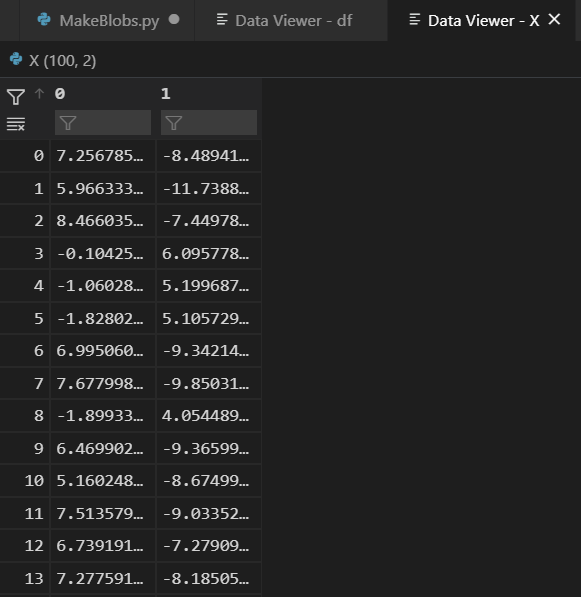
\includegraphics[scale = 0.8]{attachment/chapter_1/Scc161}
	\caption{Die Variable $X$ sieht mit $n_features = 2$ wie folgt aus}
\end{figure}

\begin{figure}[H]
	\centering
	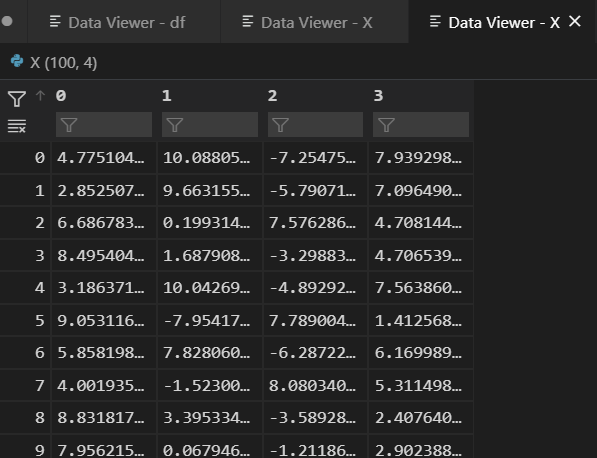
\includegraphics[scale = 0.8]{attachment/chapter_1/Scc162}
	\caption{Die Variable $X$ sieht mit $n_features = 4$ wie folgt aus}
\end{figure}

Der Testdatensatz ist somit erstellt. Für die Plotung wird diese im Folgenden vorbereitet.
\begin{lstlisting}[style=Python]
	# Collect all in one df
	df = Dataframe(dict(x = X[:;0],y = X[:;1], label = y))
\end{lstlisting}\footnote{\textit{class pandas.DataFrame(data=None, index=None, columns=None, dtype=None, copy=False)}
	\begin{itemize}
		\item \textbf{data} ndarray (structured or homogeneous), Iterable, dict, or DataFrame\\
		Dict can contain Series, arrays, constants, dataclass or list-like objects. If data is a dict, column order follows insertion-order.
		\item \textbf{index} $\dots$
\end{itemize}} \footnote{$X[:;0]$ bedeutet, dass alle Zeile $:$ und die erste Spalte mit Index $0$ ausgewählt wird.}
\footnote{Die Funktion \textit{dict()} ließt drei Werte ein $x$, $y$ und $label$. Die Auslesung erfolgt über die Ausgabe von $X$ und $y$. Dabei wird $X[\textit{Zeile},\textit{Spalte}]$ angewandt, um die entsprechenden Werte auszulesen. Bsp.: $X[1;1] >>> -8,2313234234$
}

Für die unterschiedlichen Labels werden eine \textit{Series} erstellt, welche verschiedenen Farben für die verschiedenen Clusters.

Für die grafische Bewertung wird eine Farbpalette zusammengestellt.
\begin{lstlisting}[style=Python]
	# scatter plot, dots colored by class value
	colors = {0:'red', 1:'blue', 2:'green',3:'yellow'}
\end{lstlisting}
 % Intro Clustering: K-Means

%\section{azureml-core (Python SDK)}
% I want to be this guy, who builds with his team an increatiable A.I: system for munich.

\subsection{Connect to Workspace}
A workspace is a resource, which is tied (child) to a subscription and a resource group. A workspace links the different object to run a \gls{ML} model: Experiment, Training, Deployment. A workspace comes with a \gls{SDK} to interactive with.\\

To connect to the workspace, the constructor requires different parameters
\begin{lstlisting}[style=python]
	Workspace(
	subscription_id, resource_group, workspace_name,
	auth=None,
	_location=None,
	_disable_service_check=False,
	_workspace_id=None,
	sku='basic',tags=None, _cloud='AzureCloud'
	)
\end{lstlisting} 


\begin{comment}


There are different ways to connect to the workspace. 
\paragraph*{VSCode} allows for the use of a extension: \textit{Azure ML}. This allows to configure the connection by an \gls{IDE}. This allows also to use the \textit{compute instance} linked to the workspace as a \gls{VM}.\\

For this a kernel needs to be selected. 
%%
\paragraph{sdfsdf}
%veu
%vm
%kernel

% Python interpreter -> Python Virtual Machine
% Python interpreter & compiler
% High level language (source) code
% Binary or machine code
% Python interpreter is CPython and writen in C
% PVM converts a byte code into a bit code 
% Python interpreter Pythion 3.10 (.exe file?
% Different python version are different python programmes: This programm is called the interpreter. You can interacte with it directly over the command line (Input for the programm), which "interpretes" you high-level code and returns the output, after the interpreter is converting you high-level code into machine code.* Note: A compiler has basically the same goal, but it is doining it a bit differently.
% You could alsow provide a scipt for you interpreter, which then returns the output of this script. The IDE allows you, to better develop a python script or scripts, which then in turn is calles a python programm. A better naming, would be  a *high level programm.

% Kernel: For example. A different kernel is build, maybe for interacting with different languages (own language interpreter). The IPython with the ipykernel is build to "interprete" python and markdown/latex source code. While the IDE allows to select for different 
So each \gls{VEN} installs a kernel (ipykernel) with IPyhton (Housing). 

You alsow install jupter-lab (evolution for IPyhton) in your ven

https://www.wrighters.io/using-multiple-kernels-in-jupyter/	
C:\Anaconda3
(my_env) λ jupyter --version
Selected Jupyter core packages...
IPython          : 8.9.0
ipykernel        : 6.21.1

\begin{figure}[H]
	\centering
	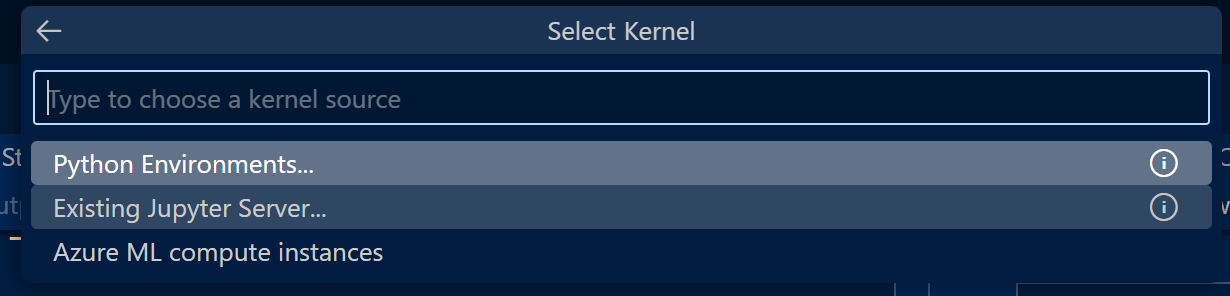
\includegraphics[scale = 0.3]{attachment/chapter_AML/Scc001}
	\caption{Connect to the workspace: Select kernel}
\end{figure}

We started, with writing the configuration file.
A started with opening jupter notebook and den selecting the kernel. And a kernel was installed on the compute cluster.
The authen

\\
auth
ServicePrincipalAuthentication or InteractiveLoginAuthentication or MsiAuthentication
default value: None
The authentication object. For more details, see https://aka.ms/aml-notebook-auth. If None, the default Azure CLI credentials will be used or the API will prompt for credentials.


\begin{lstlisting}[style=python]
	from azureml.core import Workspace
	ws = Workspace.create(name='myworkspace',
	subscription_id='<azure-subscription-id>',
	resource_group='myresourcegroup',
	create_resource_group=True,
	location='eastus2'
	)
	
	for i in range(n):
	print('i = ', i)
\end{lstlisting}


\subsection{*Kernels}
Form your local machine, you don't need to create an enviroment. You select a kernel. For this, you are not
using the local CPU to run, but you are using the compute instance. 

A bit of definition first:

Understanding a kernal an how it is connected to an environment.

Kernel: is a program that runs and introspects the user’s code.

Conda env: is a directory that contains a specific collection of conda packages that you have installed.

These 2 concepts are describing different things, kernel is like an executable, conda env is the resources (packages) at this executable’s dispose.

Selecting the compute instance, we are acturally in a visturel machine, not only a virtual enviroment. This will be 

That will be important, by selecting the compute instance, you accessing the vistural machine (which is not you local machine). Therefore the virtual envoroment will be installed over there.

For example, therefore the command write the configuration file, will create a problem. Because it seams to be, that I'm not allowed to write in the directory of the virtual machine.

Now.
the next question is, is it possible to use the internal kernal on you own machine, to excute the code.

For now, it is without the kernal form 

so the .exe in the conda enviroment is a kernal?

---- Okay, make something clean.
What I'm now testing, if i get the specific workspace configuration.
The probelm is, how do we can manage all does different access points, while having one repsository to connect to?
Questions over questions.
It is still unclear, what the difference between an interpreter and an kernel is.
For this purpose, there is no difference. it is a computional 

The \textit{IPython} with it's \textit{ipykernel} as a default kernel (as \textit{ipykernel}). 
Other language kernels are available for the jupter notebook.

IPython is XXX and ipykernel is the actually kernel. However, I still don't understand. To the question is, that 

What happen, if you select the ipykernel for in the compute instance. 
So what happens here.
The nice thing is, that I actually starting to making progress in this area.
Very, very good.

Now back. What the fuck is an interpreter, the languages it self and an kernel. The kernel think, I have the sense, it's very important, to understant. Not as a essetion question to solve it. But as a basiline knowleadge question, it seems to be nessary.

Fucking kernel.

Now, let's start anyway.

Add the pictures to

The \gls{g_Kernel} to excute the code, needs to be selected. ITE


Now, now, 

path, where the interpreter is saved?
It depends, 
The kernel is one thing, the machine, I'm running it on, is a different thing.
I need to crack it, that is this. Otherwise I'll forget it and then I will have to read up on it again.

In the beginning there was \textit{IPython}. It evolves into \textit{Jupter}, because Jupter supported more then \textit{pykernel}.

\subsubsection{Kernel}





A notebook kernel is a “computational engine” that [runs] the code contained in a Notebook document. The ipython kernel, referenced in this guide, [runs] python code. Kernels for many other languages exist (official kernels).

As shown in Figure The relationship between the kernel and the notebook. the notebook is where the instructions are written but until they are sent to the Kernel the instructions will not have any effect.

	Inhalt...
\end{comment}



 % AI Goals
%\chapter{Azure ML Python Development}\label{sec:PythonDevEnv}
\setcounter{section}{0}

 % Azure ML Usage
%
\section{Deep Dive Computer Science Part}
\subsection{Understanding ipykernel}
\subsubsection{Overview Python Interpreter}
Reference: \href{https://docs.python.org/3/tutorial/interpreter.html#the-interpreter-and-its-environment}{Using the Python Interpreter}, \href{https://blog.hubspot.com/website/what-is-python-interpreter#:~:text=A%20python%20interpreter%20is%20a,and%20low%2Dlevel%20languages%20are.}{What Is a Python Interpreter?}\\


\paragraph{High-Level Language}
The \gls{g_Python} language is a high-level programming language. This means, that the programming language is more similar to human language then to machine language, which is written in strings of bits - ones and zeros.
The advantage of it is that it is better understood by humans, but the same can not be said for the machines. Writing commands (instruction) in lines of zeros and ones is more difficult, that using higher level concepts. The gap between this, gets closes by the \textbf{Python Interpreter}.\\

The \gls{g_PyI} reads the command written by the \gls{g_Python} programmer, evaluates them, and returns the output. If the \textit{python.exe} application/ interpreter is opened, either through the \gls{CMD}, for example  
\begin{lstlisting}[language=iCMD]
	$ python3.12
	///Python 3.12 (default, April 4 2022, 09:25:04)
	///[GCC 10.2.0] on linux
	///Type "help", "copyright", "credits" or "license" for more information.
	>>>
\end{lstlisting}
the commands
\begin{lstlisting}[language=iCMD]
	>>> the_world_is_falt = True
	>>> if the_world_is_flat:
			print("Be careful not to fall off!")
	/// Be careful not to fall off!
\end{lstlisting}
or by opening the application directly.
\begin{figure}[H]
	\centering
	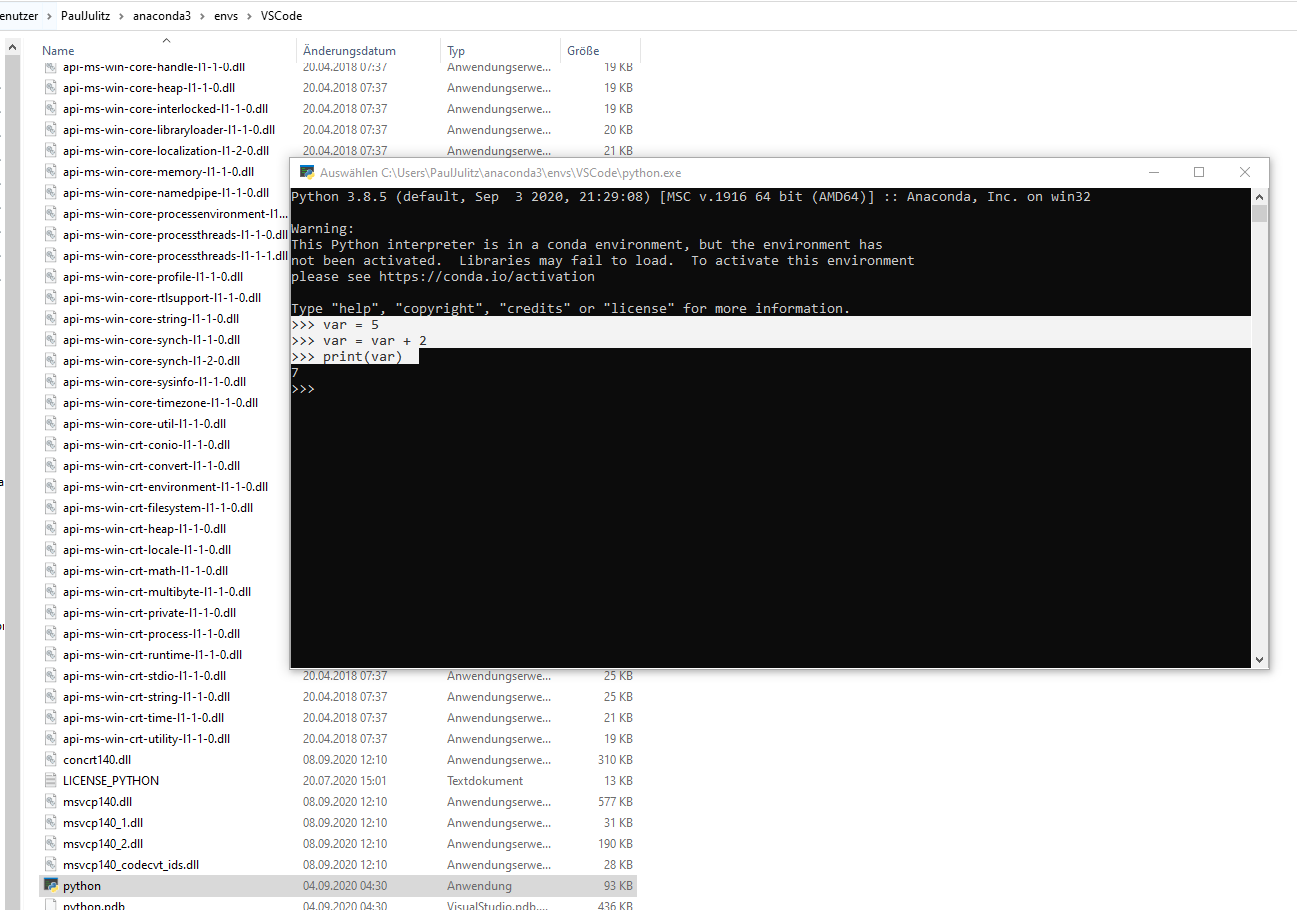
\includegraphics[scale = 0.2]{attachment/chapter_AML/Scc003}
	\caption{Using the command line with the python application/ interpreter}
\end{figure}
In both cases, the \gls{g_PyI} receives the commands and executes them. In the case where the \gls{IDE} is to write a the Python script (aka. module or application), the scripts gets passed to \gls{g_PyI}.\\

\paragraph{Difference between interpreter and a compiler}
Both the interpreter and compiler transforms the source code into binary machine code.
The difference arise through the way they are doing it differently: The interpreter translate the source code one statement at a time. The compiler on the other hand first scans the entire programm and then translate the whole program into machine code. For more detail, see \href{https://blog.hubspot.com/website/what-is-python-interpreter#:~:text=A%20python%20interpreter%20is%20a,and%20low%2Dlevel%20languages%20are.}{What Is a Python Interpreter?} or \href{https://www.analyticsvidhya.com/blog/2021/05/choose-best-python-compilers-for-your-machine-learning-project-detailed-overview/#:~:text=What%20is%20a%20Python%20compiler,executed%20directly%20by%20a%20computer.}{Best Python Compiler}
\begin{figure}[H]
	\centering
	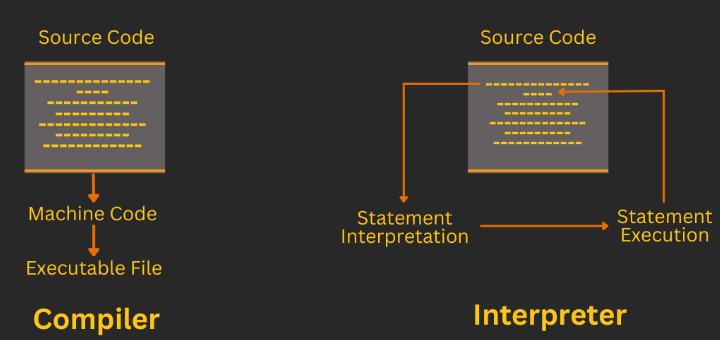
\includegraphics[scale = 0.3]{attachment/chapter_AML/Scc004}
	\caption{Example Compiler and Interpreter in Java}
\end{figure}

\subsubsection{ipykernel (Jupyter Notebook)}
Reference: \href{https://www.reddit.com/r/learnprogramming/comments/imhxai/what_is_the_difference_between_a_python_kernel_as/#:~:text=Python%20kernel%20is%20just%20a,is%20also%20not%20an%20interpreter.}{Difference Kernel and Interpreter}, \href{https://plotly.com/python/ipython-vs-python/}{IPython vs Python in Python}, \href{https://www.reddit.com/r/learnprogramming/comments/imhxai/what_is_the_difference_between_a_python_kernel_as/#:~:text=Python%20kernel%20is%20just%20a,is%20also%20not%20an%20interpreter.}{reddit:  difference between a Python Kernel (as in Jupyter notebooks) and a Python interpreter (like in PyCharm)?}, \href{https://python-forum.io/thread-40721.html}{jupyter kernel is an interface to the Python interpreter.} 


\paragraph{IPython (Python3)}
To understand the \gls{g_Kernel_Jy_Py} it is helpful to understand \textit{IPython (Notebook)}. The \gls{g_PyI} passes command to it. This only allows commands for \gls{g_Python}.\\


\textit{IPyhton} creates an interactive command line terminal for \gls{g_Python}.  

\begin{figure}[H]
	\centering
	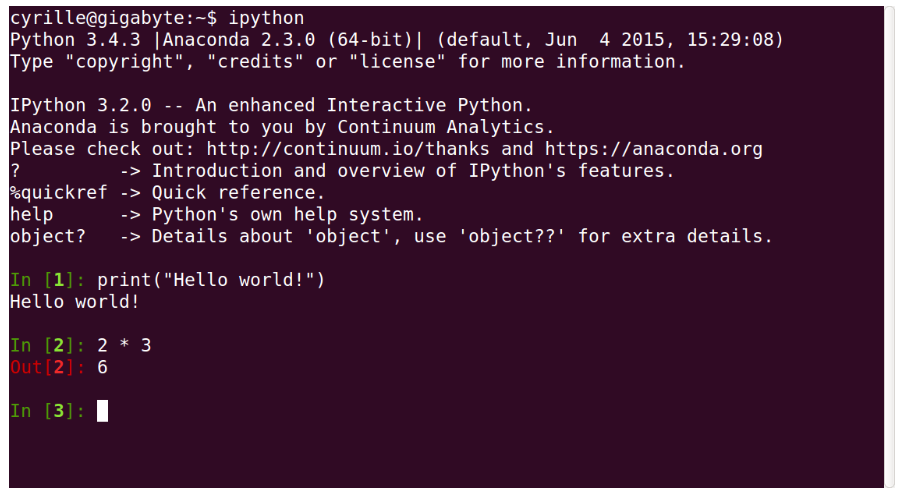
\includegraphics[scale = 0.3]{attachment/chapter_AML/Scc005}
	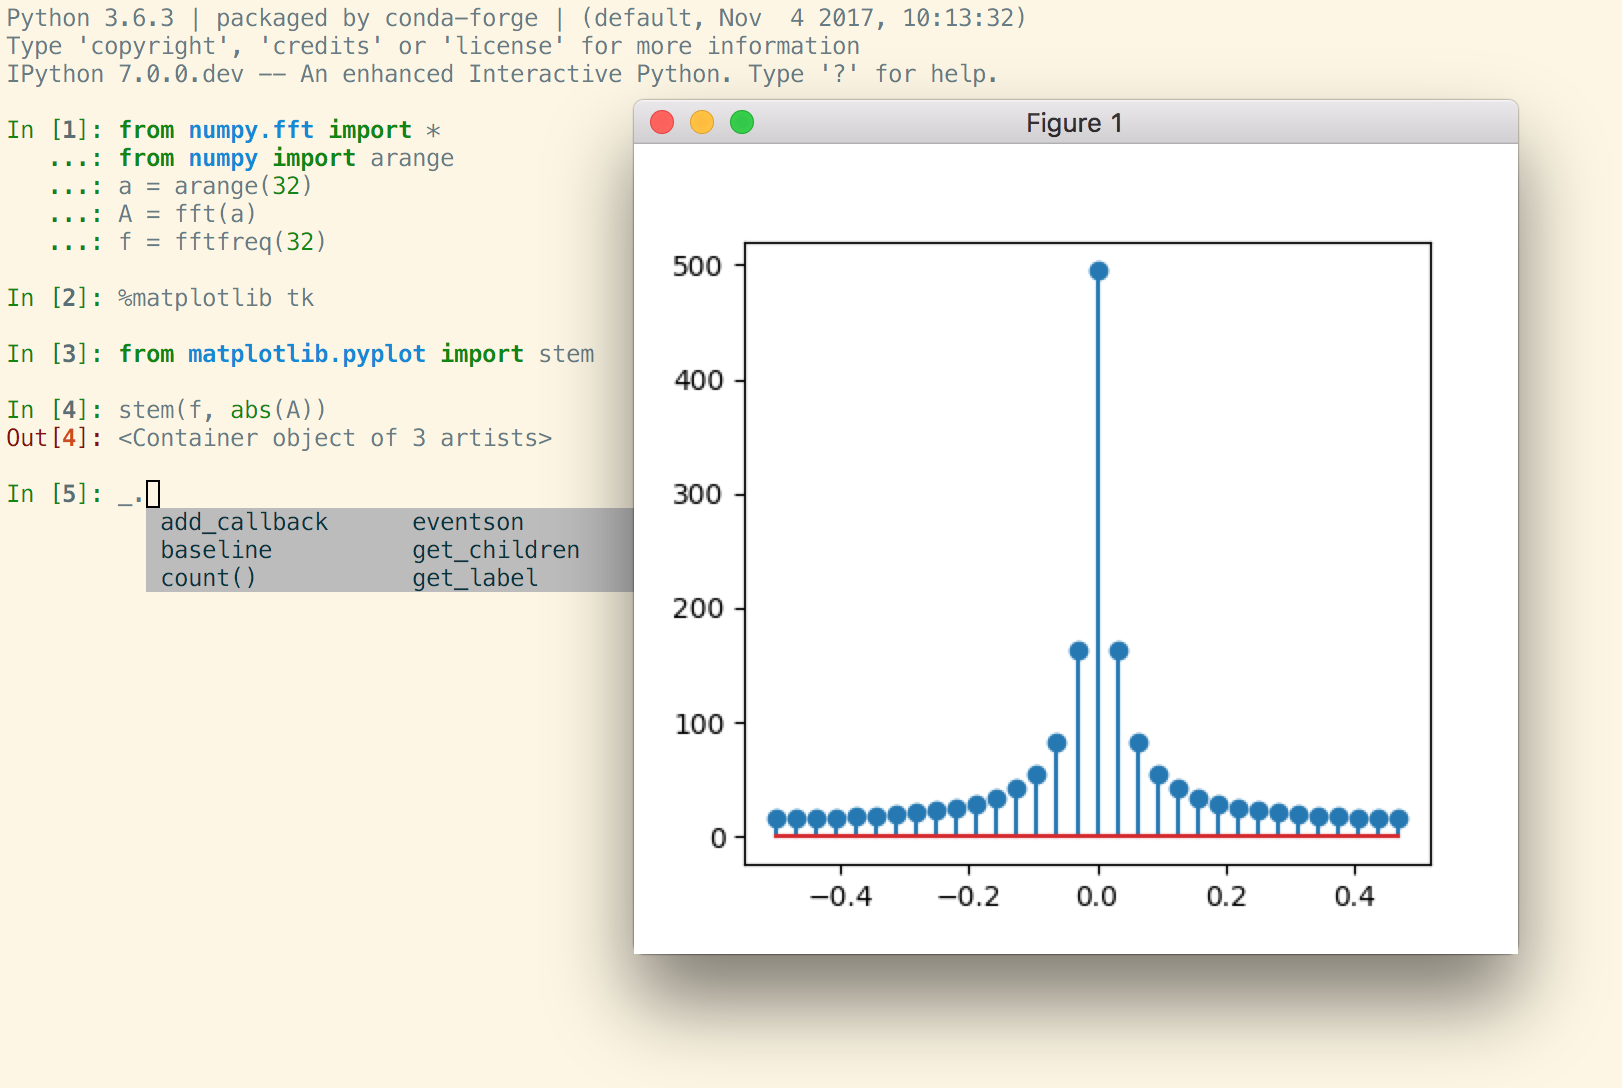
\includegraphics[scale = 0.2]{attachment/chapter_AML/Scc009}
	\caption{IPython interactive command-line terminal}
\end{figure}

\paragraph{Jupyter Notebook}
With the reorganization of \textit{IPython}, the new tool \textbf{Notebook} has been created. Under the project name \textbf{Jupyter}. This \gls{g_JupyterNotebook} is a web interface for \gls{g_Python}. It has the same interactive interface kept. Being a web-interface, it can integrate with many of the existing web libraries for data visualization.\\

The concept of a \textit{kernel} comes into play as the engine behind the web interface. The \textit{IPython} is now the backend with the \gls{g_Kernel_Jy_Py} for \gls{g_Python}. The \gls{g_Kernel_Jy_Py} with the advent of \gls{g_JupyterNotebook} is able to handel \textit{markdown} and \LaTeX text input.\\
\begin{figure}[H]
	\centering
	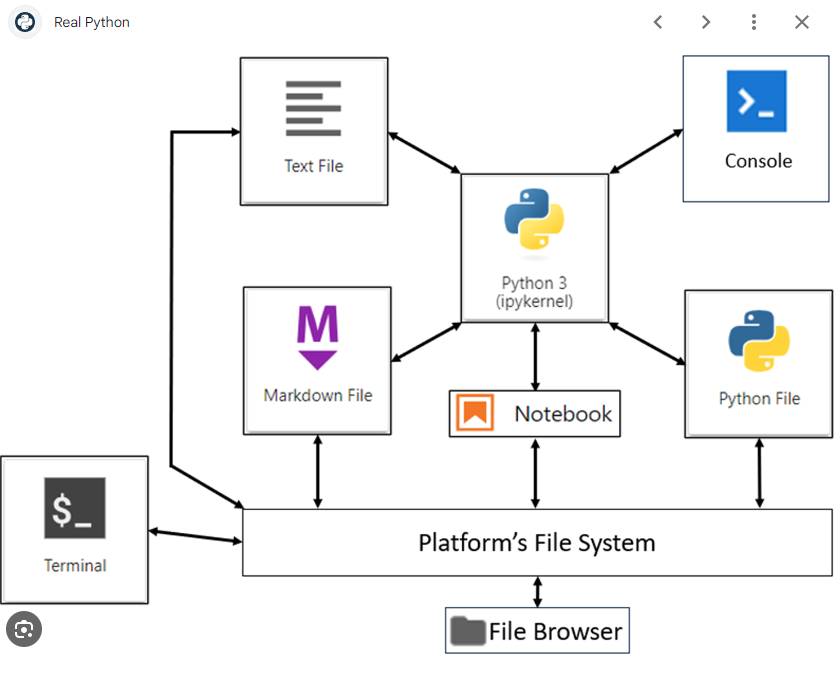
\includegraphics[scale = 0.3]{attachment/chapter_AML/Scc006}
	\caption{JupyterLab for an Enhanced Notebook, \href{https://realpython.com/using-jupyterlab/}{Jupyter Lab}}
\end{figure}
Note: The interaction with the \gls{g_Kernel_Jy_Py} is done through the \gls{g_JupyterNotebook}. With the latest tool: \textbf{Jupyter Lab}, interaction with separate files is possible.\\

$"$Inside$"$ the \gls{g_Kernel_Jy_Py} lives the \gls{g_PyI}. Another way of saying this is that the \gls{g_Kernel_Jy_Py} is the interface to the \gls{g_PyI}.\\

Note: \textit{Jupyter Lab} allows for a more interactive and simultaneous way to code.

\subsubsection{Interacting with different (language) Kernels}
\paragraph{Theoretical Multi languages Kernel}
As said before the \gls{g_Kernel_Jy_Py} is for interacting with the \gls{g_PyI} and the other functionality of a \gls{g_JupyterNotebook}.\\

The community around, \textit{Juypter Notebook}, the application, developed more \gls{g_Kernel_Jy} for the \gls{g_JupyterNotebook}. Those \gls{g_Kernel_Jy} allows to interact with different languages like \textit{Ruby, Scale, R}.\\

It would be possible (Unclear how) to create a \gls{g_Kernel_Jy} which allows to interact with all those languages in one \gls{g_JupyterNotebook}. The current research for this chapter could not found one. For example the \gls{g_Kernel_Jy_Py} allows us to interact for example with \gls{g_Python}, Markdown, Shell Script. This does not conclude for example \gls{SQL}.

\paragraph{VSCode Compute Cells Confusion}
If a \gls{g_JupyterNotebook} is open, for each cell it is possible to select the language for this cell. This those two things. First it changes the \textit{IntelSence} syntax highlights. Secondly, it provides the \gls{g_Kernel_Jy} information about the lanuage which is used in this cell.

\begin{figure}[H]
	\centering
	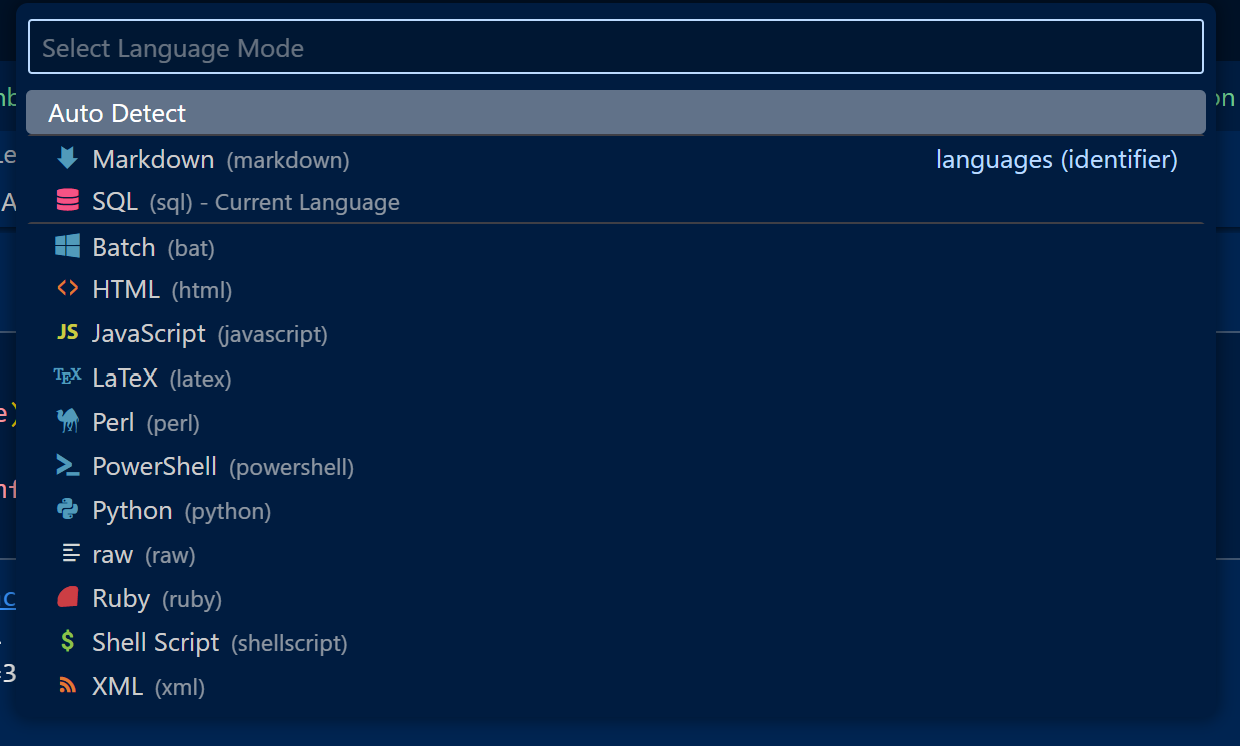
\includegraphics[scale = 0.3]{attachment/chapter_AML/Scc007}
	\caption{Cell Language Mode selection.}
\end{figure}

However, this \underline{does not mean} that all languages are supported by the selected \gls{g_Kernel_Jy}. 

\paragraph{Azure Data Studio}
In Azure Data Studio you can connect to different \gls{g_Kernel_Jy}, \href{
https://learn.microsoft.com/en-us/azure-data-studio/notebooks/notebooks-guidance?view=sql-server-ver15}{Azure Data Studio}:
\begin{itemize}
	\item \gls{SQL} Kernel,
	\item PySpark3 and PySpark Kernel,
	\item Spark Kernel,
	\item Python Kernel (for local development)
\end{itemize}


\subsubsection{VEN and ipykernel}
% Spun up by Jupyter 
% Spn up on your machine
\paragraph{Spinning Up Jupyter Notebook with Anaconda}
\begin{itemize}
	\item First a \gls{g_conda} \gls{VEN} gets created.
	\item The Jupyter Notebook $"$application$"$ gets installed
\end{itemize}
This in turn will install the package for the web interface, \textit{IPython} and the default \gls{g_Kernel_Jy_Py} for \gls{g_Python}.
\begin{lstlisting}[language=iCMD, caption={pip commands to get ready for Jupyter Notebok},captionpos=b]
	pip install jupyter
\end{lstlisting}
This command will import all dependence to work with a \gls{g_Kernel_Jy_Py}. An example of package environment see below.

\begin{lstlisting}[style=CMD, caption={Example Jupyter Notebook conda ven},captionpos=b]
	PS C:\Users\PaulJulitz\iCloudDrive\TexMaker\GitHub_Notizen_DSci\Notizen_DSci> conda list
	# packages in environment at C:\Users\PaulJulitz\anaconda3\envs\VSCode:
	#
	# Name                    Version                   Build  Channel     
	...
	azure-common              1.1.28                   pypi_0    pypi      
	azure-core                1.27.1           py38haa95532_0  
	azure-identity            1.12.0                   pypi_0    pypi      
	azure-keyvault-secrets    4.6.0                    pypi_0    pypi      
	azureml                   0.2.7                    pypi_0    pypi      
	...
	ipykernel                 5.3.4            py38h5ca1d4c_0
	ipython                   7.27.0           py38hd4e2768_0
	ipython_genutils          0.2.0              pyhd3eb1b0_1
	...
	jupyter_client            7.0.1              pyhd3eb1b0_0
	jupyter_core              4.8.1            py38haa95532_0
	jupyter_server            1.4.1            py38haa95532_0
	jupyterlab                3.2.1              pyhd3eb1b0_1
	jupyterlab_pygments       0.1.2                      py_0
	jupyterlab_server         2.8.2              pyhd3eb1b0_0
	...
\end{lstlisting}


\paragraph{Multiple Kernel (Python)}
If the setup is done through the Anaconda interface (\gls{g_conda}). The complete installation is done by Anaconda if the \gls{IDE} \gls{g_JupyterNotebook} is installed. By default \textit{IPython} is installed with the \gls{g_Kernel_Jy_Py}.\\

The command for the installation of the \gls{g_Kernel_Jy_Py} is
\begin{lstlisting}[language=iCMD, caption={pip to install ipykernel},captionpos=b]
	pip install ipykernel
\end{lstlisting}
For example to use \text{Scala}, \href{https://community.databricks.com/t5/data-engineering/how-can-we-run-scala-in-a-jupyter-notebook/td-p/17752}{Link}:
\begin{lstlisting}[language=iCMD, caption={Using Scala for a Notebook},captionpos=b]
	# Install the package
	pip install spylon-kernel
	# To select the kernel in the notebook, create a kernel spec
	python -m spylon_kernel install
	# Start Jupyter Notebook
	ipython notebook
\end{lstlisting}
In the notebook the kernel can be selected. The command is to list the available kernels is
\begin{lstlisting}[language=iCMD, caption={pip to install ipykernel},captionpos=b]
	$ jupyter kernelspec list
	>>>>Available kernels:
	>>>>python2.7        /Users/jakevdp/.ipython/kernels/python2.7
	>>>>python3.3        /Users/jakevdp/.ipython/kernels/python3.3
	>>>>python3.4        /Users/jakevdp/.ipython/kernels/python3.4
	>>>>python3.5        /Users/jakevdp/.ipython/kernels/python3.5
	>>>>python2          /Users/jakevdp/Library/Jupyter/kernels/python2
	>>>>python3          /Users/jakevdp/Library/Jupyter/kernels/python3
\end{lstlisting}
See, \href{https://stackoverflow.com/questions/39007571/running-jupyter-with-multiple-python-and-ipython-paths}{Running Multiple Kernel} for understand how to select a \gls{g_Kernel_Jy} throught the command line.
% English
% for or to?-----
% She studied FOR the exam. "For" indicates the goal, which should be achived.
% She went TO study. "to" indicates the use of a purpose before a infinit verb.

To see which \gls{g_Kernel_Jy} is running, run the following code
\begin{lstlisting}[language=iPython]
	import sys
	print(sys.executable)
	print(sys.version)
	print(sys.version_info)
\end{lstlisting} 

\subsubsection{Connecting a Notebook to a Compute Ressources}
%\paragraph{Locally}
To use a \gls{g_JupyterNotebook}, the web interface creates either a
\begin{itemize}
	\item local server,
	\item or provides the possibility to connect to a Jupyter hosted server.
\end{itemize}
Note: The local server is still your own machine.\\

The packages for connecting to a server are installed in the \gls{VEN}. The "spinning" up is basically the configuration to either a local port on your machine or to a hosted server. The former is used for computing.

\begin{figure}[H]
	\centering
	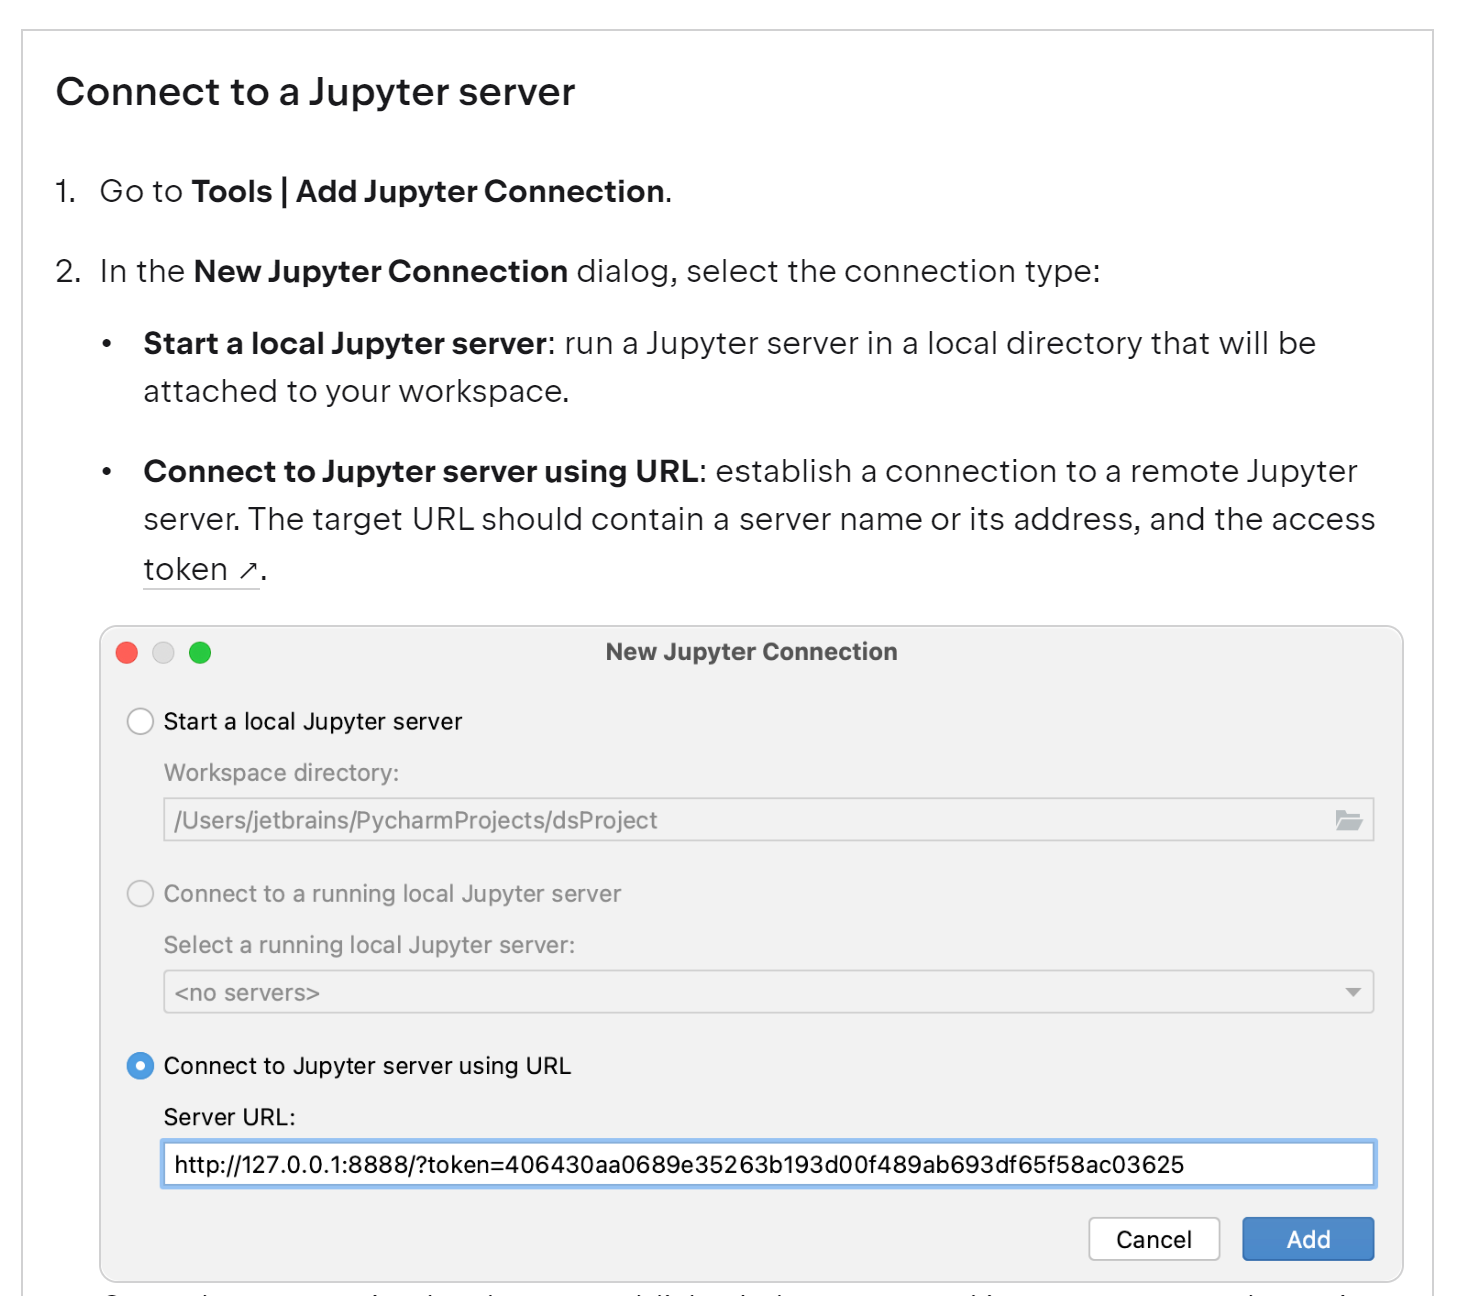
\includegraphics[scale = 0.3]{attachment/chapter_AML/Scc008}
	\caption{Mac Setup of Jupter Notebook Server}
\end{figure}

If the notebook should be connected to the compute cluster, this is done by a SHH Tunnel.

\begin{figure}[H]
	\centering
	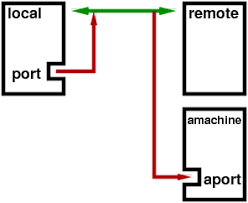
\includegraphics[scale = 0.3]{attachment/chapter_AML/Scc010}
	\caption{Tunnel Trafic, \href{https://radcamp.github.io/AF-Biota/Jupyter_Notebook_Setup.html}{SHH Tunnel}}
\end{figure}

\subsection{Setting Up the Environment}

\subsubsection{Working with conda}
\paragraph{Interacting with conda from the terminal}
Here are three ways to interact with the python interpreter:
\begin{description}
	\item[conda comand] Starting the \textit{Anaconda Navigator} and start the \gls{IDE} from there. This then allows to interact with conda throug the \textbf{conda} \textbf{Cmdlet} from the terminal.
	
	\item[PowerShell Extension] If the local machine has some restriction, that prohibist the use of the command \textbf{conda} from the powershell terminal.
	\begin{figure}[H]
		\centering
		\includegraphics[scale = 0.3]{attachment/chapter_AML/Scc023}
		\caption{Terminal Response by using conda command}
	\end{figure}
	Still, the following powershell script allows when execute to use a \textit{powershell extension}, that bypass this problem.
	\begin{lstlisting}[language=iCMD, caption={.ps1 script}, captionpos=b]
		#region conda initialize
		# !! Contents within this block are managed by 'conda init' !!
		$varPath  = "C:\User\" + (Get-ChildItem Env:USERNAME).Value + "\anaconda\Scripts\conda.exe"
		If (Test-Path $varPath ) {
			(& $varPath  "shell.powershell" "hook") | Out-String | ?{$_} | Invoke-Expression
		}
		#endregion
	\end{lstlisting}
	This powershell extension allows you with the \gls{g_conda} program.
	\begin{figure}[H]
		\centering
		\includegraphics[scale = 0.2]{attachment/chapter_AML/Scc026}
		\caption{PowerShell Extension}
	\end{figure}
	One restriction still exists. In \gls{vsc} the option to run a program requires to create a python terminal in which the \textbf{conda} command can be access. This will not work, because a new terminal will be created in which the \textbf{conda} command can't be access. However, the python interpreter in a specific \gls{g_conda} \gls{VEN} can still be access by providing the direct path to it.
	\begin{figure}[H]
		\centering
		\includegraphics[scale = 0.4]{attachment/chapter_AML/Scc027}
		\caption{PowerShell Extension and Python Interpreter}
	\end{figure}
	\begin{lstlisting}[language=iCMD, caption={Commands}, captionpos=b]
		(base) PS C:\Users\PaulJulitz\Documents\GitHub\Emmy_ML_One> conda activate Icarus_v3
		(Icarus_v3) PS C:\Users\PaulJulitz\Documents\GitHub\Emmy_ML_One> & C:/Users/PaulJulitz/anaconda3/envs/Icarus_v3/python.exe c:/Users/PaulJulitz/Documents/GitHub/Emmy_ML_One/test.py  
		Hello
		None
		(Icarus_v3) PS C:\Users\PaulJulitz\Documents\GitHub\Emmy_ML_One>
	\end{lstlisting}
	\item[Pointing to the interpreter] If the conda command can't be used.
	Then the python interpreter it self can be selected.
	\begin{figure}[H]
		\centering
		\includegraphics[scale = 0.4]{attachment/chapter_AML/Scc025}
		\caption{Selecting the python interpreter in \gls{vsc}}
	\end{figure}
	Running a python script will use the python interpreter inside the selected \gls{g_conda} \gls{VEN}.
	\begin{figure}[H]
		\centering
		\includegraphics[scale = 0.2]{attachment/chapter_AML/Scc024}
		\caption{Terminal Response by using the python interpreter}
	\end{figure}
\end{description}

\subsubsection{Good Practices for Constants, Configuration and Secrets}
% constant class, see work from Sebastian
% .env is a local file, that allow you to work with secrets and configuration, which you mirrow in the cloud, because you are NOT commiting it.
% setup.sh (Unclear)

\paragraph{.env files (Local Configuration)}
The \textit{.env} has the purpose to store locally secrets and configuration, which are not allowed to commit to the repository. The variable names in his file need to be setup in \gls{CI}/\gls{CD} processes as well, for example in a variable group for a testing pipeline.

\paragraph{Configuration}
To limited scope control a good practices is to store constant in a separate file: : \verb+util/constant.py+.\footnote{See commend out href
	%\href{https://medium.com/@zeid.zandi/how-to-manage-constants-in-python-best-practices-and-advanced-techniques-50fa1591d517#:~:text=Constants%20in%20Python%20are%20typically,access%20and%20modification%2C%20if%20necessary}{How to Manage Constants in Python: Best Practices and Advanced Techniques}
}

Constant defined in a separate file can be imported and accessed from any part of the code base. 


\begin{lstlisting}[language=iPython, caption={Installing Azure ML SDK core package},captionpos=b]
	class Setting:
	"""
	Settings that can be used to change the code behavior.
	"""
	# If False Live paths from configuration.yaml will be used
	TEST_ENVIRONMENT = True
	
	# IF True log  containing already read pvn reports will be deleted so all found pvn files will be used again
	CLEAR_ALREADY_READ_LOG = True
	
	# Determinants wich output will be written
	ENABLE_EINZELBUCHUNGEN_REPORT = True
	ENABLE_KENNZAHLEN_REPORT = True
	ENABLE_KONTEN_REPORT = True
	
	# Codes that will be read by EINZELBUCHUNGEN and determent the output of the report
	CODES: list = ['41', '42', '56', '80', '81', '82', '83', '84', '88']
	# In order to prevent unexpected behavior all codes that might have rows with empty dates should be added here
	CODES_WITH_EMPTY_ROWS: list = ['41', "56"]
\end{lstlisting}

Combined this with separate class for constant and utizizing \textit{Enum} improves some of the drawbacks.
\begin{lstlisting}[style=Python, caption={Installing Azure ML SDK core package},captionpos=b]
# Constants classes
class MathConstants:
PI = 3.14159


class AppConfig:
MAX_SIZE = 100
MIN_SIZE = 10


# ConstantsManagement class
class ConstantsManagement:
def __init__(self):
# Set constants from separate classes as attributes
for cls in [MathConstants, AppConfig]:
for key, value in cls.__dict__.items():
if not key.startswith("__"):
self.__dict__.update(**{key: value})

def __setattr__(self, name, value):
raise TypeError("Constants are immutable")

# Create an instance of ConstantsManagement
constants_manager = ConstantsManagement()

# Accessing constants
print(constants_manager.PI)  # Output: 3.14159
print(constants_manager.MAX_SIZE)  # Output: 100

# Attempting to modify constants raises a TypeError
#constants_manager.PI = 3.14  # Raises TypeError: Constants are immutable
\end{lstlisting}


\subsection{Azure.ai.ml Class}
\subsubsection{azure.ai.ml.Input}\label{subsec:azure-ai-ml-Input}
This module can be imported \verb+from azure.ai.ml import Input+, see \href{https://learn.microsoft.com/de-de/python/api/azure-ai-ml/azure.ai.ml.input?view=azure-python}{azure.ai.ml.input Doc}.
\paragraph{Class Constructor}
\begin{lstlisting}[language=iPython,  caption={Konstrukor},captionpos=b]
	Input(*, type: Literal['uri_folder'] = 'uri_folder', path: str | None = None, mode: str | None = None, optional: bool | None = None, description: str | None = None, **kwargs)
\end{lstlisting}
This constructor of the class \verb+Input()+ stores the input values in an dictionary. Therefore, they can be access in the same way.
\begin{lstlisting}[language=iPython,  caption={Exmample Usage Input()},captionpos=b]
	input = Input(
		type="uri_file",
		path="https://azuremlexamples.blob.core.windows.net/datasets/diabetes.csv",
		)
	)
	print(input.get("type")) # -> "url_file"
	print(input["type"]) # -> "url_file"
\end{lstlisting}

\paragraph{Literal} type are are a standard of the \href{https://peps.python.org/pep-0586/}{PEP 484 ecosystem}. \textit{Literal types} indicate that some expression has literally a specific value. This allows in the above example to control the input value for the argument \textit{type}.
\begin{lstlisting}[language=iPython,  caption={Exmample Usage Input()},captionpos=b]
from typing import Literal

def accepts_only_four(x: Literal[4]) -> None:
ic(x)

ic(accepts_only_four(4))   # OK - pass mype
ic(accepts_only_four(19))  # Rejected, mypy will throughs an error
\end{lstlisting}

\begin{lstlisting}[style=CMD]
ic| x: 4
ic| x: 19
4
19
\end{lstlisting}

The constructor \verb+Input()+ will use a literal type hint to explain, that for option are available inputs for the argument \verb+type=+
\begin{itemize}
	\item \verb+"uri_folder"+
	\item \verb+"uri_file"+
	\item \verb+"mltable"+
	\item \verb+"mltflow_model"+
	\item \verb+"custom_model"+
	\item \verb+"string, integer, boolean"+
\end{itemize}
Depending on the input eigher this function of the next usage will be effected by it.
 % ipykernel
%\section{Using Azure ML API/ SDK/ CLI}
\subsection{Overview}
The following
\subsection{Basics}
\paragraph{SDK vs. CLI}
The \gls{g_Python} \gls{AMLSDKv2} with the package library
\begin{center}
	\textbf{azure-ai-ml}
\end{center}
and the \gls{AMLSDKv1} with 
\begin{center}
	\textbf{azureml-core}
\end{center}
are \gls{API}s for the \gls{AML} workspace and it's services. The \gls{CLI} package for \gls{AML} contains a more compact command line style workflows, that need to be executed. The format in v2 is normally <noun><verb><option>.\\

The \gls{SDK} is more directed to the development, while the \gls{CLI} is more convient for a \gls{CI}/\gls{CD} process. The later is due to the more compact way of executing commands.\footnote{Reference: \href{https://learn.microsoft.com/en-us/answers/questions/1395777/what-is-the-difference-between-azure-ail-ml-and-az}{Difference CLI, SDK}, \href{https://github.com/microsoft/MLOps}{MLOps Python AML}
}

\paragraph{Working with conda}


\begin{comment}
\subsubsection{*Example SDK/ CLI}
References: \href{https://learn.microsoft.com/de-de/azure/machine-learning/how-to-setup-vs-code?view=azureml-api-2}{Start Setup VS-Code}
\href{https://learn.microsoft.com/de-de/azure/machine-learning/how-to-launch-vs-code-remote?view=azureml-api-2&tabs=vscode-desktop}{Case: VSCode Desktop}
\href{https://learn.microsoft.com/de-de/azure/machine-learning/tutorial-train-deploy-image-classification-model-vscode?view=azureml-api-2}{Tutorial: Reference SDK/CLI v2 Example Doc}
\href{https://github.com/Azure/azureml-examples/blob/main/cli/jobs/single-step/tensorflow/mnist/src/train.py}{git Repo Example SDK/CLI v2}

\subsubsection{* Utilizing other ressources in Azure ML workspace}
With both Azure and Azure ML Extension it is possible to manage the resources directly. 
%How exaclty, I'll see.
\begin{figure}[H]
	\centering
	\includegraphics[scale = 0.3]{attachment/chapter_AML/Scc020}
	\caption{Azure and Azure ML Extension}
\end{figure}
\end{comment}

\subsection{Running "On" the Compute Instance}
\subsubsection{Single Jupyter Notebook Connection}
Reference: \href{https://learn.microsoft.com/de-de/azure/machine-learning/how-to-launch-vs-code-remote?view=azureml-api-2&tabs=vscode-desktop}{Getting started with VS-Code Desktop}\\

With this functionality, any local \gls{g_JupyterNotebook} can use the a remote server connection to execute code on a compute instance with a \gls{g_Kernel_Jy}.\\

To run a \gls{g_JupyterNotebook}, a \gls{g_Kernel_Jy} needs to be selected.

\begin{figure}[H]
	\centering
	\includegraphics[scale = 0.3]{attachment/chapter_AML/Scc015}
	\caption{Kernel Selection in a Jupyter Notebook}
\end{figure}

In \gls{vsc}, there are multiple options to select a \gls{g_Kernel_Jy}. With the Azure ML extension, the option \textit{Azure ML Compute Instance} is available to.  On the compute instance, a variety of \gls{g_Kernel_Jy} are pre-installed.
\begin{figure}[H]
	\centering
	\includegraphics[scale = 0.3]{attachment/chapter_AML/Scc016}
	\caption{Kernel Sources}
\end{figure}

This connection allows to utilize the Azure ML Compute Instance, not all the other resource's. In the following the interaction between and to the other resources will be discussed.

\paragraph{Problem $\&$ Fix: Unable to connect}
One problem accrued. 
\begin{figure}[H]
	\centering
	\includegraphics[scale = 0.3]{attachment/chapter_AML/Scc017}
	\caption{Error message after selecting Azure ML Compute Instance}
\end{figure}

For the moment, rollback the \gls{g_JupyterNotebook} extension to a version v2023.10.xxx helped.\footnote{
	\href{https://github.com/microsoft/vscode-jupyter/issues/14925}{Posted Problem}, \href{https://github.com/microsoft/vscode-jupyter/pull/14929}{Pull Request and Workaround}
}
\begin{figure}[H]
	\centering
	\includegraphics[scale = 0.3]{attachment/chapter_AML/Scc018}
	\caption{Rollback version}
\end{figure}

\subsubsection{Tunnel Connection}
\begin{comment}
	## Unclear, how this is going to work
	
	If a tunnel is made between \gls{vsc} and the the workspace the \gls{CLI} can be access by the terminal, see \href{https://learn.microsoft.com/de-de/azure/machine-learning/how-to-work-in-vs-code-remote?view=azureml-api-2}{Using az login --identity}
	
\end{comment}
With the option to connect to the workspace it self, the blobstorage, where the notebooks of each user are stored, can be access. To to this \gls{vsc} connected via tunnel to the workspace with the compute instance in the web browser or with the desktop application.
 
\begin{figure}[H]
	\centering
	\includegraphics[scale = 0.3]{attachment/chapter_AML/Scc022}
	\caption{Create a tunnel connection}
\end{figure}

On the bottom left (1) the tunnel connection is displayed. The internal filessystem gets linked as the storage (2), where the notebook can be access. Note: Locally stored notebooks can be used by the previous section.

\begin{figure}[H]
	\centering
	\includegraphics[scale = 0.3]{attachment/chapter_AML/Scc021}
	\caption{Create a tunnel connection}
\end{figure}


\subsection{Running "with" the Compute Instance (SDK v1)}

This section will explain how to use \gls{AML} with your local computer as a compute resources.\footnote{
Reference:  \href{https://learn.microsoft.com/en-us/azure/machine-learning/how-to-configure-environment?view=azureml-api-2#local-computer-or-remote-vm-environment}{Guide Installing SDK for Local Computer}
}\\

%TODO: Setting Up a experiment, by using a compute instance 
%TODO: Setting up an experiemnt, by using local compute.
\subsubsection{Using a local kernel/ Python Interpreter}

\begin{itemize}
	\item Create a \gls{g_Python} \gls{VEN} with conda on you local computer
	\item Install the newest \gls{AMLSDKv1}.
	\footnote{
	Because the more extensive example is setup with \gls{AMLSDKv1}, we will start from here to. The idea is, that more functionally are provides by \gls{AMLSDKv2} then this will be incrementally be used. \href{https://learn.microsoft.com/en-us/python/api/overview/azure/ml/install?view=azure-ml-py}{Installation Guide}
}
	\begin{lstlisting}[style=CMD, caption={Installing Azure ML SDK core package},captionpos=b]
		pip install azureml-core
	\end{lstlisting}
	The \gls{SDK} contains many more optional packages, see \href{https://learn.microsoft.com/en-us/python/api/overview/azure/ml/install?view=azure-ml-py}{Optional Packages for Azure ML}
	\item Installing \gls{g_JupyterNotebook} required packages.
\end{itemize}

\begin{lstlisting}[style=CMD, caption={Installing Azure ML SDK core package},captionpos=b]
	conda 
\end{lstlisting} % New AI Goal: Learning Python SDK, Example of own simple Model

\chapter{Artifical Neural Network}
\setcounter{section}{0}
 % Artifical Neural Network
\section{Objective}

Reference: \href{https://youtu.be/TkwXa7Cvfr8?si=V8cJG_DQAoA2fndE}{Watching Neural Networks Learn}

An \gls{AI_NN} is a \textit{non-linear mathematical tool} intended to simulate the human brain process by using simple units called artificial neurons arranged in structures known as layers.
\begin{center}
	An \gls{AI_NN} is a \textit{universal function approximator}. They are machines that create functions.
\end{center}

This non-linear mathematical tool can also be understood as a \textit{universal function approximator}. The \textit{Universal Approximation Theorem} states that \gls{AI_NN} with infinite neurons can approximate any function given the right weights. How to achieve this or how to come closer should be the objective of this segment. For example, the layer architecture, the activation function, and preparing the data are relevant topics to consider for finding the global minimum.

\paragraph{Different ways to look at it}
Many mathmatical field are in interplay when it comes to a \gls{AI_NN}.\\

Linear Algebra is mostly used when it comes to computing information though the network. Graph Theory can also be used to to the same thing, but is mostly considered when it comes to analyzing the structure of the neural network. 

\begin{description}
	\item[Linear Algebra] \glspl{AI_NN} can be represented using matrices and vectors, where each neuron's input and output can be described as linear combinations of the inputs with corresponding weights. Matrix operations such as multiplication, addition, and transposition are fundamental in understanding how information flows through the network during forward and backward propagation.
	\item[Graph Theory] \glspl{AI_NN} can be represented as directed graphs, where neurons correspond to nodes and connections between neurons correspond to edges. Graph theory concepts are useful for analyzing the structure of neural networks, including connectivity patterns and network architectures.
\end{description}

Given a certain structure of the network \textit{optimisation} with main tool from \textit{calculus}: \textit{gradient descent} is used to find the parameter that reduces the loss function.\footnote{
	While calculus and optimization are related and often used together in the context of machine learning and neural networks, they are distinct mathematical concepts with different focuses.
}

\begin{description}
	\item[Optimization] \gls{AI_NN} are trained by optimizing a loss function with respect to the network's parameters. Optimization theory provides a framework for selecting appropriate optimization algorithms, tuning hyperparameters, and understanding convergence properties. While calculus provides the mathematical framework for computing gradients and understanding the behavior of optimization algorithms, optimization theory encompasses a wider range of techniques beyond calculus, such as convex optimization, linear programming, and heuristic algorithms.
	\item[Calculus (Optimization)] Calculus is essential for optimizing the parameters (weights and biases) of \gls{AI_NN} through techniques like gradient descent and its variants. Understanding derivatives is crucial for computing gradients, which indicate how the loss function changes with respect to changes in the network's parameters. Calculus helps in finding the direction and rate of change that minimizes or maximizes a function, which is crucial for training neural networks to minimize the loss function.
\end{description}

The field of \textit{probability and statistics} as well as \textit{information theory} are used for multiple aspects of \glspl{AI_NN}. For example the former can be used to preparing or preprocessing of data, model evaluation and bringing into context the uncertainty in predictions. The later will also be used for finding the features in the dataset as well as analysing the information flow inside a \gls{AI_NN}.

\begin{description}
	\item[Probability and Statistics] ANNs can be viewed as probabilistic models, especially in the context of Bayesian neural networks, where uncertainty is explicitly modeled. Statistical techniques are used for data preprocessing, model evaluation, and uncertainty estimation in predictions.
	\item[Information Theory] Information theory concepts, such as entropy and mutual information, can be used to analyze the information flow within neural networks. Compression techniques inspired by information theory, such as autoencoders, are used for feature extraction and dimensionality reduction.
\end{description}

The field of \textit{functional analysis} provides the tools to analyze the natrue of the universal function approximator, called \gls{AI_NN}.

\begin{description}
	\item[Functional Analysis] \glspl{AI_NN} can be viewed as function approximators, and functional analysis provides tools for analyzing the properties of these approximations. Understanding function spaces and convergence properties is relevant when studying the expressive power and generalization abilities of neural networks. 
\end{description}

\begin{sidewaystable}[h] %!ht
	\centering
	\begin{tabular}{|p{3cm}|*{6}{p{3cm}|}}
		\hline
		\textbf{Mathematical Fields} & \textbf{Featurization} & \textbf{Data Processing} & \textbf{Model Architecture} & \textbf{Optimization Parameter} & \textbf{Evaluation} & \textbf{General Assessment} \\ \hline
		\textbf{Linear Algebra} & ~ & ~ & ANN represented as matrices and vectors; Input and Output linear combination & ~ & ~ & ~ \\ \hline
		\textbf{Graph Theory} & ~ & ~ & ANN represented as directed graphs; Analyzing the structure of the network & ~ & ~ & ~ \\ \hline
		\textbf{Information Theory} & Compression techniques: autoencoder; dimensionality reduction & ~ & ~ & ~ & ~ & ~ \\ \hline
		\textbf{Optimization (e.g., Calculus)} & ~ & ~ & ~ & Techniques like gradient descent and weights and biases & ~ & ~ \\ \hline
		\textbf{Probability Theory (Stochastic)} & ~ & Techniques for data processing steps & In case of a BNN & ~ & Model evaluation; uncertainty estimation in predictions & ~ \\ \hline
		\textbf{Functional Analysis} & ~ & ~ & ~ & ~ & ~ & Understanding the expressive power/general ability \\ \hline
	\end{tabular}
	\caption{Workflow Diagram of Mathematical Perspectives in ANN}
\end{sidewaystable}

\paragraph{Landscape of different Architectures}

There are different kinds of \gls{AI_NN}, for example: convolutional, recursive. This segment will focus on \textit{feed-forward} networks. A Feed-Forward is usually a non-linear regression or classification with a sigmoidal activation and a multilayer perceptron.

\begin{figure}[H]
	\centering
	\includegraphics[scale = 0.1]{attachment/chapter_AML/Scc035}
	\caption{Types of artificial neural networks.}
\end{figure}

\section{Multilayer Perceptrons (MLP)}

\paragraph{Mathematical Foundations}
Reference, siehe auskommentierte Link und dem Buch \cite{MLK_Andr_Buk}[93] % \href{https://www.mdpi.com/2075-1680/11/2/80#:~:text=Hence%2C%20each%20artificial%20neuron%20may,b%20)%20%2C%20see%20Figure%201.}{https://www.mdpi.com/2075-1680/11/2/80#:~:text=Hence%2C%20each%20artificial%20neuron%20may,b%20)%20%2C%20see%20Figure%201.}
\begin{description}
	\item \gls{AI_NN}: Nonlinear Mathematical Tools as Universal Function Approximators
	\item Each node combines an \textit{affine linear function} and a nonlinear \textit{activation function}. 
\end{description}

\glspl{AI_NN} are nonlinear mathematical tools\footnote{However, there is a possibility to design it so that it can be a linear function.}, intended to mimic human brain processes by stacking simple neurons together. The simplest unit of an \gls{AI_NN} is called a \textit{Neuron}. They are structured in \textit{layers}. The learning process for humans is called training, while for \glspl{AI_NN} it is referred to as training.

A layer can be represented as a \textit{parameterized function}. From the perspective of a directed graph, each node can be represented as an \textit{affine linear function}. The combination of each layer can be understood as a new \textit{affine linear function} [for a given neuron].

The nonlinear quality of an \gls{AI_NN} arises from the \textit{activation function}.

\paragraph{Transformer Function} Given the input $x^t$\footnote{
	The initial input of the layer can be understood as \textit{features}, which can be represented as a vector  $x^t = (x_1, \dots, x_n)$
}. These are processed in a \textit{neuron} through \textit{weights} $w_i, i=1,\dots, n$, producing $z$, which then produces the final output $y$ through some function $\phi$, $\phi(z) = y$.

The output $z$ is the result of processing the $n-x_i$ weightily:
\begin{align}
z &= (w_1, \dots, w_n) \left(\begin{matrix}
		x_1 \\
		\vdots \\
		x_n
	\end{matrix} \right) + b \\
  &= \sum_{i=1}^n x_i\cdot w_i +b = w^t x + b,
\end{align}
where $b$ is called \textit{bias}. This should give the system more flexibility by imitating a human filter. This \textit{affine function} can be changed into a linear function, where $b$ is set as $w_0$ and $x_0 = 1$:
\begin{align}
z &= (w_0, \dots, w_n) \left(\begin{matrix}
		x_0 = 1 \\
		\vdots \\
		x_n
	\end{matrix} \right) \\
  &= \sum_{i=0}^n x_i\cdot w_i = w^t x.
\end{align}
To avoid the notation of the transpose, it can be represented by $w\cdot x$.

However, depending on the needs, these processes can be viewed as affine or linear functions. In either case, processing the input $x_i$ resulting in $z$ is called a \textbf{transfer function}. Depending on the needs different transformers can be used. The most popular or most used is the sum operator $\sum$:

\begin{figure}[h]
\centering
\begin{tikzpicture}
    % Nodes
    \foreach \x/\name in {1/x_1, 2/x_2, 3/. .. , 4/x_{n-1}, 5/x_n}
        \node at (0,-\x*0.5) (x\x) {$\name$};
  
    
    %% Node (e.g. Boxes, Symboles)    
    % Transformer Box
     \node[draw, minimum width=2cm, minimum height= 2.2 cm] at (3,-1.5) (transformer) {\shortstack{Transformer Function\\ Example: $\sum_{i=0}^n $\\ $z = w\cdot x + b$}};
    
    
    % Output activation symbole
    \node[right of=transformer, node distance=4cm] (z) {$z = w\cdot x + b$};
    
    
    %% Arrows
    % *0.5 reduces the distance
    \foreach \x in {1,2,...,5}*0.5
        \draw[->] (x\x.east) -- ([xshift=-2pt]transformer.west |- x\x);
    \draw[->] (transformer.east) -- (z.west);

    
\end{tikzpicture}
\caption{One perceptron, aka neuron}
\end{figure}

\paragraph{Activation Function}
The function $y=\phi(z)$ is known as the \textit{activation function} and it is this function that is resonsible for the non-linearity of the process. The function can be $"$freely$"$ selected, if it is fullyfilling certain criteria. \\

Each neuron can be regared as a mathematical function that is changing the \textit{transformation function} and the \textit{activation} with the inputs togehter: $y=\phi(z)= \phi\left(wx+b\right)$:

\begin{figure}[h]
\centering
\begin{tikzpicture}
    % Nodes
    \foreach \x/\name in {1/x_1, 2/x_2, 3/. .. , 4/x_{n-1}, 5/x_n}
        \node at (0,-\x*0.5) (x\x) {$\name$};
  
    
    %% Node (e.g. Boxes, Symboles)
	 % Activation Box
    \node[draw, minimum width=2cm, minimum height= 1 cm] at (8.5,-1.5) (activation) {\shortstack{Activation Function \\ $y = \phi(z)$}};
    
    % Transformer Box
     \node[draw, minimum width=2cm, minimum height= 2.2 cm] at (3,-1.5) (transformer) {\shortstack{Transformer Function\\  $\left(\sum_{i=0}^n \right)$\\ $z = w\cdot x + b$}};
    
    
    % Output activation symbole
    \node[right of=activation, node distance=3cm] (phi) {$y = \phi(z) $};
    
    
    %% Arrows
    % *0.5 reduces the distance
    \foreach \x in {1,2,...,5}*0.5
        \draw[->] (x\x.east) -- ([xshift=-2pt]transformer.west |- x\x);
    \draw[->] (transformer.east) -- node[below] {$z$}(activation.west);
    \draw[->] (activation.east) -- (phi.west);

    
\end{tikzpicture}
\caption{One perceptron, aka neuron}
\end{figure}

\pagebreak
\paragraph{Feed-Forward}

As discussed before, the entirety of \glspl{AI_NN} can be understood as mathematical functions with an input $x$ and an output $y$.

\begin{align}
	f_{NN}(x) = y
\end{align} 

To combine each neuron, the output of each neuron is sent to all neurons in the next layer. This forwarding of information is called \textit{feed-forward}. From the perspective of a function, this is called \textit{verschachteln}. Each neuron in each layer (hidden layer) receives the output of the previous neurons. This neuron is then called a \gls{MLP}.

\begin{Definition}{Multilayer Perceptron}
	
	A \gls{MLP} is a function $f_l:\R^n \rightarrow \R$. It is called an $n-L-m$ perceptron, with $n$ inputs, $L$ hidden layers, and $m$ outputs.
	
	\begin{align}
		y = f^{(l)}(\vec{x}) = f_{l-1}\left(f_{l-2}\left(...\left(f_{0}(\vec{x})\right)\right)\right).
	\end{align}
	
	Where $f^{(i)}(\vec{z}) \stackrel{def}{=} \phi_l\left( \Matrix[W]^{(l)}\vec{z} + b^{(l)}\right)$.
\end{Definition}


\begin{figure}[h]
	\centering
\scalebox{0.6}{%
	\begin{tikzpicture}
		
		% Drawing input on the left side each input layer
		\def\movefactorZeroZeroCircles{-7.5}
		\foreach \x/\layerindex in {1/x}{
			\foreach \y/\neuroindex in {6/1,4/2}{
				\node[name=\layerindex_\neuroindex] at (\x*3.25 +\movefactorZeroZeroCircles -0.8125,\y*0.75) {% function desciption
					$x_\neuroindex$
				};
				
			}
		}
		
		% Input layer with two neurons
		\draw[dotted] (-4.5,0) rectangle ++(2,7);
		\node at (-3.5,7.5) {Input Layer}; % Label for the Hidden layer one
		
		% Drawing circles on the left side of the Hidden layer one
		\def\movefactorZeroCircles{-6}
		\foreach \x/\layerindex in {1/0}{
			\foreach \y/\neuroindex in {6/1,4/2}{
				\filldraw[fill=green!20, draw=green!50!black] (\x*3.25 +\movefactorZeroCircles -0.8125,\y*0.75) circle circle (0.4);
				\node[name=\layerindex_\neuroindex] at (\x*3.25 +\movefactorZeroCircles -0.8125,\y*0.75) {% function desciption
					$x^{(\layerindex)}_{\neuroindex}$
				};
			}
		}   
		
		% Hidden layer one with four neurons
		\draw[dotted] (0,0) rectangle ++(5,7);
		\node at (2.5,7.5) {Hidden Layer One}; % Label for the Hidden layer one
		
		% Drawing neurons and displaying function in the Hidden layer one
		\foreach \x/\layerindex in {1/1}{
			\def\forwardedlayerindex{0}
			\foreach \y/\neuroindex in {8/1,6/2,4/3,2/4}{
				\fill[blue!20] (\x*3.25 -2.9,\y*0.75-0.375) rectangle ++(4.2,0.75);
				\node[name=\layerindex_\neuroindex] at (\x*3.25-0.8125,\y*0.75-0.375+0.375) {% function desciption
					$y_\neuroindex^{(\layerindex)} \leftarrow g_\layerindex \left(\vec{w}^{(\layerindex)}_{\neuroindex}\vec{x}^{(\forwardedlayerindex)}+b_{\layerindex,\neuroindex}\right)$
				};
			}
		}
		
		% Second box with four neurons
		\draw[dotted] (6,0) rectangle ++(5,7);
		\node at (8.5,7.5) {Hidden Layer Two}; % Label for the second box
		
		% Drawing neurons and displaying function in the second box
		\def\movefactorSecondBox{6}
		\def\forwardedlayerindex{1}
		\foreach \x/\layerindex in {1/2}{
			\foreach \y/\neuroindex in {8/1,6/2,4/3,2/4}{
				\fill[pink!20] (\x*3.25 + \movefactorSecondBox -2.9,\y*0.75-0.375) rectangle ++(4.2,0.75);
				\node[name=\layerindex_\neuroindex] at (\x*3.25+ \movefactorSecondBox -0.8125,\y*0.75-0.375+0.375) {% function desciption
					$y_\neuroindex^{(\layerindex)} \leftarrow g_\layerindex \left(\vec{w}^{(\layerindex)}_{\neuroindex}\vec{y}^{(\forwardedlayerindex)}+b_{\layerindex,\neuroindex}\right)$
				};
			}
		}
		
		% Third box with a single inner box
		\draw[dotted] (12,0) rectangle ++(5,7);
		\node at (14.5,7.5) {Output Layer}; % Label for the third box
		
		% Drawing neurons and displaying function in the third box
		\def\movefactorThirdBox{6}
		\def\forwardedlayerindex{2}
		\foreach \x/\layerindex in {1/3}{
			\foreach \y/\neuroindex in {5/1}{
				\fill[red!20] (\x*3.25 + \movefactorSecondBox + \movefactorThirdBox -2.9,\y*0.75-0.375) rectangle ++(4.2,0.75);
				\node[name=\layerindex_\neuroindex] at (\x*3.25+ \movefactorSecondBox + \movefactorThirdBox -0.8125,\y*0.75-0.375+0.375) {% function desciption
					$y_\neuroindex^{(\layerindex)} \leftarrow g_\layerindex \left(\vec{w}^{(\layerindex)}_{\neuroindex}\vec{y}^{(\forwardedlayerindex)}+b_{\layerindex,\neuroindex}\right)$
				};
			}
		}
		
		% Arrows connecting right side of input to left side of the corresponding cicle
		\draw[->] (x_1) -- (0_1);
		\draw[->] (x_2) -- (0_2);
		
		% Arrows connecting right side of circels to left side of the corresponding inner box of the Hidden layer one
		\foreach \x in {1,2}
		\foreach \y in {1,2,3,4}
		\draw[->] (0_\x.east) -- (1_\y.west);
		
		
		% Arrows connecting right side of neurons of the Hidden layer one to left side of the corresponding inner box of the second box
		\foreach \x in {1,2,3,4}
		\foreach \y in {1,2,3,4}
		\draw[->] (1_\x.east) -- (2_\y.west);
		
		% Arrows connecting right side of neurons of the second box to left side of the single inner box of the third box
		\foreach \x in {1,2,3,4}
		\foreach \y in {1}
		\draw[->] (2_\x.east) -- (3_\y.west);
		
		% Arrow from right side of inner box of the third box to slightly outside the dotted line with label y on the right hand side
		\draw[->] (3_1.east) -- (6+\movefactorSecondBox+\movefactorThirdBox,5*0.75) node[right] {$y$};
		
		
		
	\end{tikzpicture}
}
\caption{\gls{MLP} with two hidden layer, one input vector and one output layer}
\end{figure}


In this example, the output of the \gls{MLP} $y^{(1)}_1$ is calculated by the activation function $g_1$ for the hidden layer $1$. The weight vector $\vec{w}^{(0)}_1$ has dimension $2$, as it receives two inputs $x^{(1)}_1$ and $x^{(1)}_2$, along with the scalar bias $b^{(1)}_1$. In the next layer, the dimension of each weight vector is $4$, as each \gls{MLP} receives inputs $y^{(1)}_1$, $y^{(1)}_2$, $y^{(1)}_3$, and $y^{(1)}_4$ from the previous layer.

 % Mathmatical Fundation
\section{Application: Person Course}
\subsection{Creating a Experiment}

Or simpler: Just import jupter notebook
\begin{markdown}
Using azureml.core
\end{markdown}

\begin{lstlisting}[style=python]
import azureml.core
from azureml.core import Workspace

ws = Workspace.from_config()
print('Ready to use Azure ML {} to work with {}'.format(azureml.core.VERSION, ws.name	
\end{lstlisting}



\subsection{Hyperparameter Tuning} 

%TODO: Do this after section for batch is ready

%\subsection{Discrete and Continuous Hyperparameter}
%\subsection{SDK Use}

%TODO: STOP

\subsubsection{Batch vs. Mini Batch Size gradient descent}

The training set get's split into smaller \textit{batches}.



 % Application: Person Course


%Backlog %%%




%% Computer Science  %%%%%%%%%%%%%%%%%%%%%%%%%%%%%%
%\part{Computer Science} 
 
%%%%%%%%%%%%%%%%%%%%%%%%%%%%%%%%%%%%%%%%%%%%%%%%%%%
%)\pagebreak
\chapter{Version Controll}
\setcounter{section}{0}

\section{GitHub Introduction}
\subsection{Befehle}
\begin{description}
	\item[my-slide Verzeichnis] % C:\Users\PaulJulitz\Documents\GitHub\github-slideshow %%% HP 
	\item[my-slide Verzeichnis] % C:\Users\Paul J\Documents\GitHub\github-slideshow %%% Dell 
	\item[git ls-files] Zeigt alle Dateien in einem Verzeichnis an.
	\item[copy con <file>] Dieser Befehl funktioniert unter Git bash. Die entsprechenden Datei wird in den aktiven Verzeichnis erstellt.
	\item[git status] Gib alle Änderungen eines Verzeichnises wieder.
	\item[git clone <URL.git>] Das URL mit .git wird in dem aktiven Verzeichnis geklont.
	\item[git branch <name>] Ein neuer Branch wird im lokalen Bereich erzeugt.
	\item[git checkout <local branch>] Ändert den aktiven lokalen Branch.
	\item[git push --set-upstream origin <Branch>] Der erzeugte Branch wird zum Remote Repository geladen.
	\item[git pull orign <Branch>] Ein Update (pull) eines spezifischen Branch wird gezogen.
	\item[git branch --all] Alle Branches lokal und remote werden angezeigt.
	\item[git branch -m <Name>] Der Name des Branches, welcher gerade aktiv ist, kann mit dem Befehl geändert werden.
	\item[git -add <file>] Bereitet Änderungen aus dem Working Bereich für den nächsten Commit vor.
	\item[git commit -m $"\dots "$] Mit jedem Commit wird ein Snapshot der Dateien gemacht. Diese werden unter \gls{VCS} abgespeichert. Eine Nachricht in notwendig.
	\item[git push] Alle Commit werden für den ausgewählten Branch gepusht.
	\item[git pull origin <Branch>] Aktualisiert den spezifischen Branch.
	\item[git merge <Branch>] Der Master Branch wird mit dem ausgewählten Branch vereinigt.
	\item[git branch -d <Branch>] Löscht den lokalen Branch, welcher schon mit master vereinigt ist.
	\item[git branch -D <Branch>] Löscht den lokalen Branch.
	\item[git push origin  --delete <Branch>] Löscht den remote Branch, solang er auf \gls{g_Git} Hub noch nicht $"$archiviert$"$ wurde, sonst kann der Branch nicht gefunden werden. 
	\item[git remote prune origin] Löscht leere Branch Hüllen.
\end{description}

\subsection{Unterschied zwischen git bash, cmd und gui}
\begin{description}
	\item[Git bash] Es handelt sich hier um eine UNIX \gls{g_Shell}. Dies bietet sich an, wenn Linux schon bekannt ist.
	\item[Git CMD] Es handelt sich hier um eine UNIX \gls{g_Shell}. Dies bietet sich an, wenn Windows bekannt ist.
	\item[Git GUI] Bietet die Funktionalität von git in einer grafische Oberfläche an.
\end{description} \cite{stackoverflow.Diff}

\subsubsection{Staging Area / Index / Cache}
Der Staging Bereich oder Index erlaubt inhaltlich verbundenen Dateien/ Änderungen an Dateien aus dem Working Bereich vorzuhalten und per \textbf{git add}. 
\begin{lstlisting}[style=CMD]
	C:\Users\Paul J\Documents\GitHub\github-slideshow> git status
	On branch dell_Branch
	Your branch is up to date with 'origin/dell_Branch'.
	
	Untracked files:
	(use "git add <file>..." to include in what will be committed)
	_ <@\textcolor{red}{posts/test-dell.md}@> - Copy.txt

	nothing added to commit but untracked files present (use "git add" to track)
\end{lstlisting}
Dateien, welche diesem Index zugeordnet wurden, werden per \textbf{git commit} mit einer Nachricht zum lokalen \gls{g_Git_Repository} übertragen. Die gesammelten Commits können per \textbf{git push} zum Remote Repository übertragen werden.
\begin{lstlisting}[style=CMD]
C:\Users\Paul J\Documents\GitHub\github-slideshow> git status
On branch dell_Branch
Your branch is ahead of 'origin/dell_Branch' by 1 commit.
(use "git push" to publish your local commits)

nothing to commit, working tree clean
\end{lstlisting}
\begin{figure}[H]
	\centering
	\includegraphics[width=0.7\linewidth]{attachment/chapter_6/Scc000}
\end{figure}

Eine Datei im \gls{g_Git} Ordner kann in zwei Kategorien untergliedert werden:
\begin{itemize}
	\item tracked und
	\item untracked.
\end{itemize}
In früheren \gls{g_Git} Versionen konnte eine ungetrackte Datei \gls{g_Git_Repository} zugeordnet werden ohne als \textit{staged} markiert zu werden, sodass sie Teil der \gls{VCS} wurde. Mit \textbf{git add <file>} wird diese Datei heute zum Staging Bereich zugeordnet und von \gls{g_Git} getrackt. Beim nächsten \textbf{git push} wird diese Datei ans Remote \gls{g_Git_Repository} gesendet.


Mit \gls{g_Git} GUI ist eine Übersicht gegeben, welche Dateien noch nicht im Stage Modus sind und welche schon. 
\begin{figure}[H]
	\centering
	\includegraphics[width=0.7\linewidth]{attachment/chapter_6/Scc001}
\end{figure}
Die Commits werden pro Branch aufgeteilt.
\begin{figure}[H]
	\centering
	\includegraphics[width=0.7\linewidth]{attachment/chapter_6/Scc003}
\end{figure}
Zu jedem Schritt exisitert ein Befehl in \gls{g_Git_CMD}.
\begin{figure}[H]
	\centering
	\includegraphics[width=0.7\linewidth]{attachment/chapter_6/Scc002}
\end{figure}

\subsubsection{Commiting}
Commits sind Snapshots/ Milestones des Projektes/ Ordners oder Dateien. Dies werden werden auf dem lokalen \gls{g_Git_Repository} abgespeichert. Commits können auch wieder gelöscht werden. Wenn alle Commits bereit sind, geteilt zu werden, können sie per \textbf{git push origin <Branch>} auf das remote \gls{g_Git_Repository} geladen werden. 
Über \gls{g_Git} Hub stehen die Veränderungen und die History bereit zur Bearbeitung.

\begin{figure}[H]
	\centering
	\includegraphics[width=0.7\linewidth]{attachment/chapter_6/Scc004}
	\caption{Richtig Auswahl des Branches $\&$ History anzeigen lassen.}
\end{figure}

\begin{figure}[H]
	\centering
	\includegraphics[width=0.7\linewidth]{attachment/chapter_6/Scc005}
	\caption{Zu jedem Milstone/ Linie besteht die Möglichkeit Kommentare anzubringen.}
\end{figure}

\subsection{Example: github-slideshow}
\subsubsection{Clone Respository and Create a Branch}
Ziel in diesem Abschnitt ist es, das 
Mit der Clone Anweisung wird das \gls{g_Git_Repository} auf den lokalen Server des Users gespielt. Die \gls{VCS} wird in Git hinterelegt und speichert die Änderungen an den Daten. Damit die Änderungen sich einfach einbinden lassen und von verschiedenen User erstellt werden, wird ein \textbf{Branch} erstellt. 

\begin{lstlisting}[style=CMD]
	/// Change directory to where the repository should be saved
	git cd C:\Users\PaulJulitz\Documents\GitHub
	/// Clone repository to local server (.../Username/NameRepository)
	git clone https://github.com/pauljulitz/github-slideshow.git /// 
	/// Navigate to the repository in your shell
	git cd C:\Users\PaulJulitz\Documents\GitHub\github-slideshow
	/// Create a new branch
	git branch my-slide
\end{lstlisting}

\subsubsection{Check all the branches of one repository}
In einem \gls{g_Git_Repository} können mehrere Branches erstellt werden. Welche für das gewissen \gls{g_Git_Repository} zugewissen sind, kann über \bl{branch --all} in einen \gls{g_Git_Repository} dargestellt werden.

\begin{lstlisting}[style=CMD]
	C:\Users\PaulJulitz>cd C:\Users\PaulJulitz\Documents\GitHub\github-slideshow
	
	C:\Users\PaulJulitz\Documents\GitHub\github-slideshow> git branch --all
	master
	*<@\textcolor{green}{my-slide}@>
	secoundBranch
	<@\textcolor{red}{remotes/origin/HEAD}@> -> origin/master
	<@\textcolor{red}{remotes/origin/master}@>
	<@\textcolor{red}{remotes/origin/my-slide}@>
	<@\textcolor{red}{remotes/origin/secoundBranch}@>
\end{lstlisting}

Der aktuelle Branch wird in \textcolor{green}{Grün} mit eine $*$ angezeigt.

\subsubsection{Chance branch name}
Mit dem Befehl \textbf{-m <new name>} kann der Name des lokalen, ausgewählten Branch geändert werden. Wenn jedoch der gleiche Name für einen Branch ausgewählt wurde, wird der Zusatz \textit{-lokal} angefügt.
\begin{lstlisting}[style=CMD]
	C:\Users\PaulJulitz\Documents\GitHub\github-slideshow> git branch -m newName
\end{lstlisting}
\subsubsection{Change aktiv branch}
Ein Branch kann mit \textbf{git checkout <local branch>} gewechselt werden.
\begin{lstlisting}[style=CMD]
C:\Users\PaulJulitz\Documents\GitHub\github-slideshow> git branch --all
master
* <@\textcolor{green}{my-slide}@>
secoundBranch
<@\textcolor{red}{remotes/origin/HEAD}@> -> origin/master
<@\textcolor{red}{remotes/origin/master}@>
<@\textcolor{red}{remotes/origin/my-slide}@>
<@\textcolor{red}{remotes/origin/secoundBranch}@>

C:\Users\PaulJulitz\Documents\GitHub\github-slideshow> git checkout secoundBranch
Switched to branch 'secoundBranch'
Your branch is up to date with 'origin/secoundBranch'.

C:\Users\PaulJulitz\Documents\GitHub\github-slideshow> git branch --all
master
my-slide
* <@\textcolor{green}{secoundBranch}@>
<@\textcolor{red}{remotes/origin/HEAD}@> -> origin/master
<@\textcolor{red}{remotes/origin/master}@>
<@\textcolor{red}{remotes/origin/my-slide}@>
<@\textcolor{red}{remotes/origin/secoundBranch}@>
\end{lstlisting}

\subsubsection{Push new local branch}
Mit \textbf{--set-upstream origin <branch>} wird der angesteuerte Branch hochgeladen.
\begin{lstlisting}[style=CMD]
	git push --set-upstream origin my-slide
\end{lstlisting}

\subsubsection{Check the status of a branch}
Der Befehl \textbf{git status} gibt an, 
\begin{itemize}
	\item welcher Branch aktuell aktiv ist, 
	\item ob es Änderungen im Origion Projekt gibt und
	\item welche Änderungen gepusht werden müssen.
\end{itemize}

\begin{lstlisting}[style=CMD]
	C:\Users\PaulJulitz\Documents\GitHub\github-slideshow> git status
	On branch secoundBranch
	Your branch is up to date with 'origin/secoundBranch'.
	
	nothing to commit, working tree clear
\end{lstlisting}

\subsubsection{Create a new file}
Unter Git CMD wird der Befehl \textbf{copy con} nicht ausgeführt. Der Befehl \textbf{ls} ebenso nicht. Mit  

\subsubsection{Update Branch}
Mit dem Befehl \textbf{git pull origin <branch>} wird der spezifische Branch aktualisiert.
\begin{lstlisting}[style=CMD]
C:\Users\PaulJulitz\Documents\GitHub\github-slideshow> git pull origin my-slide
remote: Enumerating objects: 10, done.
remote: Counting objects: 100% (10/10), done.
remote: Compressing objects: 100% (7/7), done.
remote: Total 8 (delta 3), reused 0 (delta 0), pack-reused 0
Unpacking objects: 100% (8/8), 1.46 KiB | 14.00 KiB/s, done.
From https://github.com/pauljulitz/github-slideshow
* branch            my-slide   -> FETCH_HEAD
d64d186..e0c65fb  my-slide   -> origin/my-slide
Updating d64d186..e0c65fb
Fast-forward
_posts/0000-01-02-PaulJulitz.md | 6 ++++++
1 file changed, 6 insertions(+)
create mode 100644 _posts/0000-01-02-PaulJulitz.md

C:\Users\PaulJulitz\Documents\GitHub\github-slideshow> git status
On branch my-slide
Your branch is up to date with 'origin/my-slide'.

nothing to commit, working tree clean
\end{lstlisting}
\subsubsection{Pull Request}
Die kann über Github selbst erfolgen: 

\begin{figure}[H]
	\centering
	\includegraphics[width=0.7\linewidth]{attachment/chapter_6/Scc006}
\end{figure}

Oder über \gls{CMD} sind die folgenden Schritte notwendig.
Der Master Branch wird aktiviert. 
\begin{lstlisting}[style=CMD]
	C:\Users\PaulJulitz\Documents\GitHub\github-slideshow> git checkout master
\end{lstlisting}
Der benötigte Branch wird über \textbf{git merge} vereinigt.
\begin{lstlisting}[style=CMD]
	C:\Users\PaulJulitz\Documents\GitHub\github-slideshow> git merge my-slide
\end{lstlisting}
Dieser muss jetzt gepusht werden.
\begin{lstlisting}[style=CMD]
	C:\Users\PaulJulitz\Documents\GitHub\github-slideshow> git push
\end{lstlisting}
Der alte Branch kann jetzt gelöscht werden.
\begin{lstlisting}[style=CMD]
	C:\Users\PaulJulitz\Documents\GitHub\github-slideshow> git branch -d my-slide
\end{lstlisting}

\subsubsection{Delete local branch}
Wenn die Veränderungen überprüft wurden und der Branch vereingt wurde, wird das Prinzip verfolgt, den Branch zu löschen. 
Wenn dies über die \gls{g_Git} Hub Plattform passt, so bleibt eine $"$Ablage$"$ weiter bestehen.
\begin{figure}[H]
	\centering
	\includegraphics[width=0.7\linewidth]{attachment/chapter_6/Scc007}
\end{figure}
\begin{lstlisting}[style=CMD]
	C:\Users\Paul J\Documents\GitHub\github-slideshow>git push origin --delete dell_Branch
	error: unable to delete 'dell_Branch': remote ref does not exist
	<@\textcolor{red}{error: failed to push some refs to 'https://github.com/PaulJulitz/github-slideshow.git'}@>
\end{lstlisting}
Wenn dies nicht getan wurde oder der Branch wieder zurückrückgesetz wurde, wird er remote Branch gelöscht, durch: 

\begin{lstlisting}[style=CMD]
C:\Users\Paul J\Documents\GitHub\github-slideshow>git branch --all
* dell_Branch
master
remotes/origin/HEAD -> origin/master
<@\textcolor{red}{remotes/origin/dell$\_$ Branch}@>
<@\textcolor{red}{remotes/origin/dell$\_$Branch$\_$II}@>
remotes/origin/master
remotes/origin/my-slide
remotes/origin/secoundBranch

C:\Users\Paul J\Documents\GitHub\github-slideshow>git pull
Already up to date.

C:\Users\Paul J\Documents\GitHub\github-slideshow>git push origin --delete dell_Branch_II
To https://github.com/PaulJulitz/github-slideshow.git
- [deleted]         dell_Branch_II

C:\Users\Paul J\Documents\GitHub\github-slideshow>git push origin --delete dell_Branch
To https://github.com/PaulJulitz/github-slideshow.git
- [deleted]         dell_Branch

C:\Users\Paul J\Documents\GitHub\github-slideshow>git branch --all
* dell_Branch
master
remotes/origin/HEAD -> origin/master
remotes/origin/master
remotes/origin/my-slide
remotes/origin/secoundBranch
\end{lstlisting}

\subsubsection{Delete remote branch}
Der Befehl ist \textbf{git push origin --delete origin/<branch>}. Dieser ist an ein Pull Request welcher den Branch im remote \gls{g_Git_Repository} löscht. Wenn dieser Branch nicht mehr existiert, kommt ein Fehler zurück.

\subsubsection{Prune deletet remote branches}
Der Befehl \textbf{git remote prune origin} löscht alle Hüllen eines Branches.

\subsection{Designing your Github Page}
Formatierung einer .md Datei. Das README.md wir als Startseite unter der Auflistung der Daten angezeigt. Dies zu Formatieren kann helfen, eine Einführung in das \gls{g_Git_Repository} zu geben.
\begin{itemize}
	\item Ein Hashtag oder mehrere Hastagss geben die Größe der Überschrift an. 
	\item Bilder aus dem Web werden per ![profile-image](https://apod.nasa.gov/...%apod/image/1907/SpotlessSunIss_Colacurcio_2048.jpg)
	eingefügt.
	\item Wenn nur ein Bildlink eingefügt werden soll, muss das \textbf{!} vor dem Platzhaltern $[\dots]$. 
	\item Die Logik von Whatsapp ist auch hier Teilweise bei .md Formartierung anzuwenden (Kursiv, Fett, List).
\end{itemize} 

\section{GitLab Introduction}
Dieser Kurs ist ein Einsteigerkurs. Im Weiteren werden nur die wichtigsten oder neuesten Erkenntnisse notiert.

\subsection{Blame}

Mit der Blame-Funktion kann der Versionsverlauf einer bestimmten Datei nachgeschlagen werden.

\begin{figure}[H]
	\centering
	\includegraphics[width=0.7\linewidth]{attachment/chapter_5/Scc009}
\end{figure}

Dabei werden die Commits und die Veränderung direkt nebeneinander angezeigt.

\begin{figure}[H]
	\centering
	\includegraphics[width=0.7\linewidth]{attachment/chapter_5/Scc008}
\end{figure}

Dies unterscheide die History Funtkion, welche nur die Commit History anzeigt.

\begin{figure}[H]
	\centering
	\includegraphics[width=0.7\linewidth]{attachment/chapter_5/Scc010}
\end{figure}

\subsection{Groups and Subgroups}
Unter Gruppen können auch Subgruppen erstellt werden. Diese dienen einen klarern Überblick zu schaffen.

\begin{figure}[H]
	\centering
	\includegraphics[width=0.7\linewidth]{attachment/chapter_5/Scc012}
\end{figure}

\subsection{Role Permissions}

\begin{figure}[H]
	\centering
	\includegraphics[width=0.7\linewidth]{attachment/chapter_5/Scc011}
\end{figure}

\subsection{Milestones}
Mehrer Issues können einem Milestone zu geordnet werden. Es gibt noch die Möglichkeit Epics zu erstellen, diese wird jedoch nicht in jedem GitLab Packet zur Verfügung gestellt.

\begin{figure}[H]
	\centering
	\includegraphics[width=0.7\linewidth]{attachment/chapter_5/Scc013}
\end{figure}
Bei einem Milestone wird ein Start- und Enddatum angefügt.

In der Darstellung eines Milestone wird auf der rechten Seite der Status über den Milestone angezeigt.

\begin{figure}[H]
	\centering
	\includegraphics[width=0.7\linewidth]{attachment/chapter_5/Scc014}
	
\end{figure}

Die Funktionsweise ist, dass über jedes erstellt Issue auch eine \textit{estimed} und \textit{spend} Zeit angegeben werden kann. Hinweis: Es können mehrer Teilaufgaben zu einem Issue erstellt werden - siehe Checkboxen.

\begin{figure}[H]
	\centering
	\includegraphics[width=0.7\linewidth]{attachment/chapter_5/Scc015}
\end{figure}


\section{*Vitural Enviroment Anaconda}

\section{Version Kontrolle Stategie}
Es gibt verschiedene Strategien wie in Programmierungsprojekt über \gls{g_Git} verwaltet werden können. Im Folgenden wird Bezug auf die Feature-Hotfix-Stategie von Vincent Driessen auf \href{https://nvie.com/posts/a-successful-git-branching-model/}{Successful git branching model} beschrieben wird.

\subsection{Verschiedene Branches}
\begin{itemize} 
\item master  (protected, stays)
\item develop (protected, stays, merge into master, default)
\item feature (branched from develop, merge into develop, delete after, syntax f$\_$)
\item hotfix (branched form master, merge in develop and master, delete after both merges)
\item release (optional)
\end{itemize}

\subsubsection{Master and Develop}
Es existieren zwei dauerhafte Branches im Repository. Dieses sind \textbf{master} und \textbf{develop}. Diese sind geschützt (protected). Die Einstellungen zu den beiden Branches sind,
\begin{itemize}
	\item dass nur der \textbf{Maintainer} Merger Pulls oder Push bewilligen kann.
	\item dass keine Commits gesendet werden können. Es kann nur ein Merge stattfinden.
\end{itemize}

Der \textbf{Default} Branch wird von master auf develop umgestellt. Dies hat den Hintergrund, dass Features auf Basis von Develop gebrancht werden sollen. Ebenso sollen fertige Feature Branches in Develop gemerget werden. In diesem Stadium kommt es zur Überprüfung, ob das Programm dies tut, was es tun soll. Erst dann, wird es in master gemergt, welcher als Produktion Branch fungiert.

\subsubsection{Feature and Hotfix}
\begin{itemize}
	\item In Feature branch, kann auch aus einem Issue heraus erstellt werden.
	\item Ebenso kann ein Pull-Request aus einem Issue erstellt werden.
	\item Feature werden erst in Develop eingepfelgt, wenn der Review Prozess abgeschlossen ist. \footnote{Wird über die Kommentare sich ausgetauscht, welche Änderungen noch hinzugefügt werden müssen. Der Autor kann daraufhin weitere Commits tätigen. Diese Prozess wiederholt sich, bis alle Anforderungen akzeptiert sind.}
	\item Um Komplikationen beim Merging zu verhindern, sollen features nicht auf die gleichen Dateien ändern.
	\item Es empfiehl sich, --no-ff bei Merge von Feature Branches zu verwenden. Dieser Befehlt erzeugt, ein neues Commit-Objekt am Ende. Diese verursacht mehr Komplexität, diese lässt jedoch zu, dass im Develop Branch nachzuvollziehen ist, welche Commits aus welchem Feature kommen.
	\item Hotfix ist ähnlich zu Feature. Dieser kann direkt von master gebrancht werden. Die Reparaturen werden dann in Master und Develop eingepflegt. Danach wird der Hotfix Branch gelöscht.
\end{itemize}


\subsection{Merging Optionen}
\gls{g_Git} bietet verschiedene Merging-Strategie. Einzelnen können dabei kombiniert oder gleich im der \gls{IDE} verwendet werden.
Im Folgenden werden 
\begin{itemize}
	\item Merge (fast forward)
	\item Merge Recursive
	\item Merge Squasch
	\item Merge --no --ff (no fast forward)
	\item Merge Rebase
\end{itemize}
behandelt.

\subsubsection{Merge (fast forward)}
Sei Develop Branch von Master am Punkt \textit{B} geteilt worden. Dies stellt die gemeinsame Basis für beider Branches dar.
Wurde daraufhin in Develop drei commits getätigt, und keiner in Master, kann durch in Merge ein natloser Übergang geschaffen werden.\\
\Gls{g_Git} wählt die Strategie eigenständig aus, welche am besten zur Situation passt.\\

Mit dem Merge Befehl wird Develop in Master übernommen. Dabei werden die drei Commits in Master übernommen. Liegt der Pointer bei Master wird Master wie folgt nach dem Merge dargestellt.
\begin{figure}[H]
	\centering
	\includegraphics[width=0.7\linewidth]{attachment/chapter_5/Scc016}
\end{figure}

Das warum hinter Merge \textit{fast forward} steht, liegt daran, dass der Pointer von Master ohne ein weiteren Commit zum Ende von Develop geführt wird, ohne ein weiteren Commit auszulösen. Diese Option besteht jedoch nur, wenn in zu mergenden Branch keine Commits getätigt werden.

\subsubsection{Merge Recursive}
Feature wurde von Master vom Commit \textit{Add new file} geteilt. In Master wurden zwei Commits \textit{m1} und \textit{m2} getätigt. In Feature befinden sich zwei Commits \textit{f1} und \textit{f2}, welche nach dem Branching commetiert wurden.\\

\begin{figure}[H]
	\centering
	\includegraphics[width=0.7\linewidth]{attachment/chapter_5/Scc017}
	\caption{Pointer auf Master M2}
\end{figure}

\begin{figure}[H]
	\centering
	\includegraphics[width=0.7\linewidth]{attachment/chapter_5/Scc018}
	\caption{Pointer auf feature f2}
\end{figure}

Dies bedeutet, unter dem Merge-Request in Master befinden sich zwei Commits.
\begin{figure}[H]
	\centering
	\includegraphics[width=0.7\linewidth]{attachment/chapter_5/Scc019}
\end{figure}

Wie angezeigt, wird ein zusätzlicher Commit zu Master generiert. 
\begin{figure}[H]
	\centering
	\includegraphics[width=0.7\linewidth]{attachment/chapter_5/Scc020}
\end{figure}
Die Option Feature zu löschen wird erst mal ausgelassen. Die Option Squasch commits findet sich unter \textbf{Merge Squash} wieder. Nachdem Feature unter master gemergt wurde, wird diese in dem Beispiel mit dem Commit \textit{a33fd106} festgehalten.

\begin{figure}[H]
	\centering
	\includegraphics[width=0.7\linewidth]{attachment/chapter_5/Scc021}
\end{figure}

In Graph wird auf Master der neue Commit angezeigt, und die f2 und f1 im Feature Branch angezeigt.

\begin{figure}[H]
	\centering
	\includegraphics[width=0.7\linewidth]{attachment/chapter_5/Scc022}
	\caption{Pointer auf Master Merge Branch feature into master}
\end{figure}

\begin{figure}[H]
	\centering
	\includegraphics[width=0.7\linewidth]{attachment/chapter_5/Scc023}
	\caption{Pointer auf Feature f2}
\end{figure}

Die individuell, veränderten Dateien zweigen in Master die zugehörigen Commits an.

\begin{figure}[H]
	\centering
	\includegraphics[width=0.7\linewidth]{attachment/chapter_5/Scc024}
\end{figure}

Die Historie zweigt alle Commits an. Mit Hinblick auf die anderen Strategien: Es wird nicht angezeigt, welcher Commit zu welchem Source Branch gehört.
\begin{figure}[H]
	\centering
	\includegraphics[width=0.7\linewidth]{attachment/chapter_5/Scc025}
\end{figure}

Wird der Feature Branch nicht gelöscht, so bleibt er weiter bestehend. Die Commits aus Master werden jedoch nicht übernommen. Weitere Commits können in Feature getätigt werden, der Commit \textit{m1} aus Master wird jedoch nicht mit übernommen. Für eine Änderung des letzten gemeinsamen Knoten wird \textbf{Rebase} verwendet.\\

Wie im Merge (fast forward) beschrieben, wählt \gls{g_Git} selbst die beste Strategie aus. In diesem Fall wählt \gls{g_Git} \textbf{Recursive Strategie} aus. Dabei wird ein Commit erstellt, welcher auf beide Branches verweist. Die Commits werden in der History unter dem Reisverschlussprinzip dargestellt. Die Strategie wird von \gls{g_Git} angewandt wenn im Sourcebranch sowie im zu commetierenden Branch Commits vorliegen.

\subsubsection{Merge Squash}
Die Option Squash 
\begin{figure}[H]
	\centering
	\includegraphics[width=0.7\linewidth]{attachment/chapter_5/Scc020}
\end{figure}
unter dem Merge von Feature, hätte alle Commits mit den jeweiligen Änderungen und aggregiert sie zusammengefasst. Alle Änderungen werden daher gebündetl in der Historie angezeigt.\\

Unter Feature$\_$4 wurden Commits f8 und f9 getätigt. Ebenso wurde in Master m7 hinzugefügt.
\begin{figure}[H]
	\centering
	\includegraphics[width=0.7\linewidth]{attachment/chapter_5/Scc034}
\end{figure}
Wir im Merge Squash ausgewählt, wird f8 und f9 zu einem Commit zusammengefasst.
\begin{figure}[H]
	\centering
	\includegraphics[width=0.7\linewidth]{attachment/chapter_5/Scc035}
\end{figure}
Weiter bleibt bestehend, dass durch die Recursive Strategy ein Commit für den Merge erstellt wird. Die Besonderheit ist, dass das Branching vom letzten Commit auf Master m7 angezeigt wird.
\begin{figure}[H]
	\centering
	\includegraphics[width=0.7\linewidth]{attachment/chapter_5/Scc036}
\end{figure}

\subsubsection{Merge --no --ff}
Mit der Option no fastward ist ähnlich des Squash Befehl ausgeführt. Die Außnahme besteht daran, ein zusätzlicher Merge Commit getätigt wird.
    \begin{figure}[H]
    	\centering
    	\includegraphics[width=0.7\linewidth]{attachment/chapter_5/Scc037}
    \end{figure}

\subsubsection{Rebase}
Mit der Funktion Rebase wird der gemeinsame, letzte Konten definiert. 

\begin{figure}[H]
	\centering
	\includegraphics[width=0.7\linewidth]{attachment/chapter_5/Scc039}
\end{figure}
Mit Rebase werden alle Comits in dem Feature Branch nach dem neuen Knotenpunkt neu commetiert.

\begin{figure}[H]
	\centering
	\includegraphics[width=0.7\linewidth]{attachment/chapter_5/Scc040}
\end{figure}
  % Version Controll
%\pagebreak
\chapter{Power BI}
\setcounter{section}{0}

\section{Working with M (Power Query) in Power BI}
\begin{description}
\item[Funktion] Eine \textbf{Funktion} ist ein mathematische Objekte, welches eine spezielle Relation, angewandt auf eine definierte Menge, ist. Dabei wir jedem Input genau ein Output zugewiesen. Um genau zusein, ist die Funktion die Abbildungsregel, das Objekte lautet Abbildung. Mann nennt Abbildungen auch Funktionen, wenn sie ein ein Tupel aus Reelen Zahlen abbildet (Check). Beispiel: $f:\R \rightarrow \R$
\item[Expression] Eine \textbf{Expression} ist ein \textbf{algebrasiche} oder \textbf{syntakische Phrase}. In Power Query spricht man von Expression und meint damit ganze Zeilen Ausdrücke. 
\item[Value] Es gibt verschiedene Datenstrukturen. Dabei können diese auch aus mehreren zusammengebaut sein. 
\end{description}

Die Datentypen in Power Query sind ähnlich zu anderen Programmierungssprachen. Es gibt jedoch Ausnahmen. Ist kein Wert für eine Zelle vorhanden, so wird Type \textbf{Null}. Weiter Datetypen werden im Folgenden beschreiben. Hierbei werden spezielle Funktionen verwandt, um diesen Wert zu erzeugen. Dabei werden bestimmt Syntaxen verlangt.\\

\subsection{Variable}
Variablen werden bei erzeugen in $M$ nicht deklariert. Eine automatische Zuweisung der Typen funktioniert über die Syntax. Für Funktionen können jedoch Typen für Inputvariablen und die Funktion selbst definiert werden.
\begin{figure}[H]
	\centering
	\includegraphics[scale = 0.3]{attachment/chapter_1/screenshot030}
	\caption{}
	\label{fig:screenshot030}
\end{figure}
\href{https://radacad.com/basics-of-m-power-query-formula-language}{Link}

\subsubsection{Variable name}
Variablen werden in Power Query, wie auch in anderen Sprachen, mit Hilfe einer Zeichenkette definiert. Es gibt jedoch die Besonderheit, das Variablennamen auch mit einem Leerzeichen definiert werden dürfen. Dafür muss der Name als String gesehen werden und mit einem $\#$ am Anfang versehen werden.
\begin{lstlisting}[style=M]
let
	#"Das ist wirklich ein Variablenname!" = 13,
	y = #"Das ist wirklich ein Variablenname!"
in
	y // Returns 13
\end{lstlisting} 

\subsubsection{Zuweisen / Syntax}
Für das Zuweisen eines Types zu einer Variablen wird der \textbf{as} Ausdruck verwandt. Wird eine Variable erzeugt ohne eine Funktion zu verwenden, erfolgt eine automatische Type-Zuweisung.
\begin{lstlisting}[style=M]
let 
	y = 1.3234 // type number
	#"Variable 2" = "Text" // type text
	#"Variable 3" = #date(1,1,1908) // Zuweisung erfolgt durch die intrinsische Funtkion date
\end{lstlisting}
Der \textbf{as} Ausdruck wird verwandt, um Input und Output von Funktionen zu definieren. 
 \begin{lstlisting}[style=M]
let
	Funktion1 = (Input as number) as number => 2 + 3
in
	Funktion1
\end{lstlisting}
Wollen wir einen Typen einer Spalte einer Tabelle ändern, so nutzen wir die

\begin{figure}[H]
	\centering
	\includegraphics[scale = 0.3]{attachment/chapter_1/screenshot033}
	\caption{}
	\label{fig:screenshot033}
\end{figure}
Die Funktion ließt eine Tabelle als Input ein. Für die Transformation wir eine \textit{Liste} benötigt. Diese benötigt jedoch für jeden Eintrag selber eine Liste, mit dem ersten Eintrag den Spaltennamen und den zweiten den zu bezeichneten Typ.
Beispiel:
\begin{figure}[H]
	\centering
	\includegraphics[scale = 0.3]{attachment/chapter_1/screenshot032}
	\caption{Eine Spalte}
	\label{fig:screenshot032}
\end{figure}

\begin{figure}[H]
	\centering
	\includegraphics[scale = 0.3]{attachment/chapter_1/screenshot034}
	\caption{Mehrere Spalten}
	\label{fig:screenshot034}
\end{figure}

\textbf{Achtung} Es können verschiednen Syntaxen verwendet werden um eine Typ zu definieren. 
\begin{figure}[H]
	\centering
	\includegraphics[scale = 0.3]{attachment/chapter_1/screenshot035}
	\caption{Mehrere Spalten}
	\label{fig:screenshot035}
\end{figure}
Dies sieht man auch im Beispiel mit mehren Spalten. Die Integer Typumwandlung erfolgt mit dem $"$Int64.Type$"$ dieser wird jedoch nicht $"$type Int64$"$ geschrieben. Für andere Typen kann diese Logik aber angewandt werden.

\subsubsection{number, text, logical}
Variablen müssen 
\begin{lstlisting}[style=M]
let
	x = 5,
	y = x + 5, 
	w = "Test Text",
	z = true,
in 
	x // Returns 
\end{lstlisting}

\subsubsection{null}
Variablen besitzen eine Ausprägung für einen Wert. Das Konzept von $"$any$"$ and $"$null$"$ wird hier nicht berücksichtigt. Diese typen können ebenfalls abgerufen werden. Dabei kann eine Funktion eine Input auf den \textit{type type} testen. 


\begin{lstlisting}[style=M]
let
	y = null // y ist vom Typ null
	w = "null" // w ist vom Typ text
	z = 0 // z ist vom Typ number
in 
	w // Return null
\end{lstlisting}

\subsubsection{Type}
Der Type \textbf{type} wird wie intrinsische Varialben mit eine Prefix deklariert. Der Prefix lautet $"$type$"$ und der Variablentype wird in $\left\lbrace \, \right\rbrace$. Für Tabellen können die Typen für die Spalten gleich mit im Tabellenkopf vermerkt werden.
\begin{lstlisting}[style=M]
let 
	x = type {number}, // Die Variable x ist vom type type.
	y = #table(
			{Column1, Cloumn2}, // Kopf der Tabelle ohne Typen
			{
				{2, "text"},
				{4, "hello"}
			}
		),

	w = #table(
			type table [Column1 = type number, Column2 = type text], 
			\\ Kopf der Tabelle mit Typen 
			{
				{2, "text"},
				{4, "hello"}
			}
		)

in
	y 
\end{lstlisting} 
\subsubsection{Intrinsiche Werte}
Um Werte wie \textit{date, duration, binary} etc. zu schaffen, werden spezielle \textbf{single intrinsic function} benötigt. Man erkennt diese daran, dass vor ihnen ein $\#$ steht. 

\begin{lstlisting}[style=M]
let
	x = #date(2019,2,2)
in
	x // Returns 2019-2-2
\end{lstlisting} 

\subsection{Strukturierte Variablen} 
Es gibt drei verschiedene Datentypen, welche aus mehreren Komponenten bestehen

erden.
\href{https://www.howtoexcel.org/power-query/m-code/}{Link}, \href{https://docs.microsoft.com/en-us/powerquery-m/expressions-values-and-let-expression}{Link}

\begin{lstlisting}[style=M]
let
	x = {a,2,abc} // List
	y = [ // Record
			variable1 = 1,
			Item = "abc,
			ID = 4
		], 
	w = #table(
			{"Column1", "Column 2" },
			{
				{2, 4},
				{"abs", 5},
				{123j,#date(2019,2,2)}
			}
in
	x{3} // Returns abc
	// y[Item] returns abs
	// w{2}[Column1] returns 123j; 2 ist die zweite Zeile (Start 0) 
\end{lstlisting} 

\subsubsection{List} Eine Liste ist ein einfaches Array, welches alle verschiedene Typen von Objekten beinhalten kann. 
\subsubsection{Record} Ein Record ist ein Array, welches zu jedem Eintrag eine Indexnamen ausweisen kann. Es können auch Records von Records gemacht werden.
\subsubsection{Table} Eine Tabelle teilt sich in den Tabellenkopf und die Zeilen auf. Um eine Table zu erstellen, muss die intrinsische Funktion $\#table()$ angewandt werden.\\

Bei der Erstellung der Tabellen, können gleich \textbf{typen} von Datenformaten gewählt werden, siehe Zuweisen/ Syntax. 

\subsubsection{Beispiele}
\begin{lstlisting}[style=M]
let  
    Source =   
{  
   1,   
   "Bob",   
   DateTime.ToText(DateTime.LocalNow(), "yyyy-MM-dd"),   
   [OrderID = 1, CustomerID = 1, Item = "Fishing rod", Price = 100.0]   
}  
in   
    Source 
\end{lstlisting}
Das Result ist: 

\begin{figure}[H]
	\centering
	\includegraphics[scale = 0.3]{attachment/chapter_1/screenshot031}
	\caption{}
	\label{fig:screenshot031}
\end{figure}


\subsection{Function} 
Eigenen Funktionen können ebenfalls geschrieben werden. Es ist jedoch die sequenzielle Natur des M-Codes zu berücksichtigen. Eine Besonderheit zur Sprache $C++$ ist, dass die Typen für Input und Output Variablen nicht dekliniert werden müssen. Es wird dann von \textbf{impliziten Funktionen} gesprochen. Der \textit{Tye any} wird dann als \textit{Default} genutzt:
\subsubsection{Implicite function}
\begin{align}
\text{Name der Funktion } = \left(\text{ Inputvariablen }\right) = > \text{Expression}, 
\end{align} 
\begin{lstlisting}[style=M]
let  
	Add = (x, y) => x + y,
	AddResualts = 
		[
			OnePlusTwo = Add(1,2) // Ergebnis ist 3
			OnePlusOne = Add(1,1) // Ergebnis ist 2
		]
in   
   AddResualts 
   /*
   OnePlusTwo 3
   OnePlusOne 2
   */
\end{lstlisting}

\subsubsection{Explicite function}
Bei dieser Art von Funktionen müsse die Typen für die Input- wie Outputvariablen angegeben werden. Dies erfolgt im zweiten Block. 
\begin{align}
\text{Name der Funktion } = \left(\text{ Inputvariablen as $"$type$"$ }\right) \text{as $"$type$"$} = > \text{Expression}, 
\end{align} 
Mit etwas geschickt, können auch komplexere Funktionen gebaut werden.

\begin{lstlisting}[style=M]
let
	GreaterThenFive = (list) =>
		let
			OrderedList = List.Select(list, each _ >= 5) 
			/*
			List.Select(list as list, selection as function) as list
			*/
			Result = List.First(OrderedList)
		in 
	Record = [
		Ergebnis1 = GreaterThenFive({1,2,6}) // Returns 6
		Ergebnis2 = GreaterThenFive({12,12,45,23}) // Returns 12
		]
in 
	Record
\end{lstlisting} 
\subsubsection{Bewertungen (Conditions)}
Es ist essentielle für das Verstehen der meisten Funktionen, wie Tabllen, Listen, Records abgerufen und Teilmengen der Informationen selektiert werden können.
\begin{description}
\item[Table]
\begin{figure}[H]
	\centering
	\includegraphics[scale = 0.3]{attachment/chapter_1/screenshot052}
	\caption{Tabelle - Zeile und Spalte (type cell-type}
	\label{fig:screenshot052}
\end{figure}
\begin{figure}[H]
	\centering
	\includegraphics[scale = 0.3]{attachment/chapter_1/screenshot053}
	\caption{Tabelle - Spalte (type list)}
	\label{fig:screenshot053}
\end{figure}
\begin{figure}[H]
	\centering
	\includegraphics[scale = 0.3]{attachment/chapter_1/screenshot054}
	\caption{Tabelle - Zeile (type record}
	\label{fig:screenshot054}
\end{figure}
\item[Record]
\begin{figure}[H]
	\centering
	\includegraphics[scale = 0.3]{attachment/chapter_1/screenshot055}
	\caption{Record - Zeile ${}$: Geht nicht!)}
	\label{fig:screenshot055}
\end{figure}
\begin{figure}[H]
	\centering
	\includegraphics[scale = 0.3]{attachment/chapter_1/screenshot056}
	\caption{Record - Eintrag [] (type cell-type}; Wichtig: Table.SelectRows()
	\label{fig:screenshot056}
\end{figure}
\item[List]
\begin{figure}[H]
	\centering
	\includegraphics[scale = 0.3]{attachment/chapter_1/screenshot044}
	\caption{Liste - Zeile (type cell-type}
	\label{fig:screenshot0}
\end{figure}
\end{description}
Eine Funktion kann als Outputwert vom \textit{type logic} sein, sie kann aber auch jeden anderen Wert annehmen. Wichtig ist jedoch, wird eine Logische Abfrage im Funktionskörper veranlasst und diese nicht verarbeitet, so nimmt die Funktion den Typen logic an.\\

Eine Funktion kann, wenn ihr eine Tabelle übergeben wird, eine Liste wieder geben, wenn aus der Tabelle eine Spalte mit $[]$ ausgelesen wird, siehe \ref{fig:screenshot032}. Wird die ausgelesene Liste verglichen mit einem einzelnen Wert, so wird die logische Abfrage \textit{false} wiedergeben, da die beiden typen nicht gleich sind.

\begin{figure}[H]
	\centering
	\includegraphics[scale = 0.3]{attachment/chapter_1/screenshot043}
	\caption{}
	\label{fig:screenshot043}
\end{figure}
Selbst wenn jeder Eintrag in der List den gleichen zuüberprüfenden Eintrag hat, gibt die Funktion \textit{false} wieder

\begin{figure}[H]
	\centering
	\includegraphics[scale = 0.3]{attachment/chapter_1/screenshot036}
	\caption{}
	\label{fig:screenshot036}
\end{figure}
Wird ein Abgleich mit einer List gemacht, welche die gleichen Einträge beinhaltet, so gibt die Funktion \textit{true} wieder.

\begin{figure}[H]
	\centering
	\includegraphics[scale = 0.3]{attachment/chapter_1/screenshot037}
	\caption{}
	\label{fig:screenshot037}
\end{figure}
Es sei vermerkt, es werden nicht die Typen abgefragt, sondern jeder Eintrag in der Liste wird verglichen.

\begin{figure}[H]
	\centering
	\includegraphics[scale = 0.3]{attachment/chapter_1/screenshot038}
	\caption{}
	\label{fig:screenshot038}
\end{figure}
Im Abschnitt \textbf{each} wir über die eine spezielle Funktion gesprochen. 
\subsection{Spezielle}
\subsubsection{Empty Variable}
Um den Ausdruck \textbf{each} verstehen zu können, sollte die Leere-Variable besprochen werden. In Phython als auch M wir $\_$ für Puffervariablen genutzt, welche später nicht mehr gebracht werden. 
\begin{lstlisting}[style=M]
let
	_ = Table.FromColumns({
		{"Fred", "Mary", "Phil", "Sue"},
		{1, 2, 3, 4},
		{5, 2, 5, 1}},
		{"Person", "Index", "Score"} // Tabellenkopf
	)
in
	_ // Die temporäre Variable heißt _ und ist vom Type table.
\end{lstlisting}

Um verschiedenen Daten von der Tabelle abzurufen, nutzen wir die Indexschreibweise:
\begin{align} 
	\text{Tabellen-Variablen-Namen}\left\lbrace\text{Zeile} \right\rbrace \left[\text{Spaltennamen}\right]
\end{align} 
Für den Variablennamen $\_$ gilt dies natürlich auch:
 \begin{lstlisting}[style=M]
let
	_ = Table.FromColumns({
		{"Fred", "Mary", "Phil", "Sue"},
		{1, 2, 3, 4},
		{5, 2, 5, 1}},
		{"Person", "Index", "Score"} // Tabellenkopf
	)
in
	_[Person] // Return Gesamte Spalte Person vom type list
	// _{2}[Person] // Return Zeile 2 der Spalte Person
\end{lstlisting}
Den temporären Variablennamen können wir auch weglassen, wenn Tabellen angesprochen werden. Dieser Prozess sollte für Listen nicht verwendet werden, da Power Query einen Zeilenverweis für Listen als neue Liste interpretiert:
 \begin{lstlisting}[style=M]
let
	_ = {"ab", null, 6}
in
	_{2} // Return null
	// {2} // Erstellen einer weiteren Liste
\end{lstlisting}

Für Tabellen kann jedoch der $\_$ weggelassen werden.

 \begin{lstlisting}[style=M]
let
	_ = Table.FromColumns({
		{"Fred", "Mary", "Phil", "Sue"},
		{1, 2, 3, 4},
		{5, 2, 5, 1}},
		{"Person", "Index", "Score"} // Tabellenkopf
	)
in
	[Person] // Return Gesamte Spalte Person
\end{lstlisting}
\subsubsection{Each}
Die Funktion \textit{each} ist eine einfache Funktion, welche die Syntax der Leeren Variable nutzt. Es gilt:
\begin{align}
\text{each }x := (\_) => \_ x 
\end{align} 
Der Begriff each ist vielleicht etwas irreführend, da nicht wirklich ein \textit{loop}-Durchlauf gestartet wird. Vielmehr wird die each-Funktion genutzt, wenn die ummantelnde Funktion den loop-Durchlauf startet und each eine Überprüfung für jede der übergebenen Element machen soll. \\

Es ist sehr wichtig zwischen Tabellen und Records zu unterscheiden. Wir der each-Funktion eine Tabelle übergeben und sie soll bewerten, ob eine Wert in jeder Zeile steht, funktioniert dies nicht mit einem einzelnen Wert

\begin{figure}[H]
	\centering
	\includegraphics[scale = 0.3]{attachment/chapter_1/screenshot039}
	\caption{}
	\label{fig:screenshot039}
\end{figure}
Auch hier gilt, es muss mit einer Liste abgeglichen werden.

\begin{figure}[H]
	\centering
	\includegraphics[scale = 0.3]{attachment/chapter_1/screenshot040}
	\caption{}
	\label{fig:screenshot040}
\end{figure}
Damit each \textit{true} zurückgeben kann, muss die geprüfte List ebenfalls die richtigen Wert enthalten.

\begin{figure}[H]
	\centering
	\includegraphics[scale = 0.3]{attachment/chapter_1/screenshot041}
	\caption{}
	\label{fig:screenshot041}
\end{figure}
Wird die Funktion \textbf{Table.SelectRows()} eingesetzt, so wir nicht eine Tabelle, sondern ein Record für die zu überprüfenden Zeile übergeben.

\begin{figure}[H]
	\centering
	\includegraphics[scale = 0.3]{attachment/chapter_1/screenshot042}
	\caption{}
	\label{fig:screenshot042}
\end{figure}

Der \textit{each} Operator nimmt das übergebenen Record-Element, welches aus der Tabelle extrahiert wurde und überprüft mit der Eintragssyntax $[]$, die auch die Spaltensyntax für Tabellen ist, den Wert der für die Zeile in der entsprechenden Spalte steht. Eine einfache logsiche Abfrage entscheidet dann, ob der Eintrag zu $"$jeder$"$ Zeile in der entsprechenden Spalten richtig ist. Wenn ja, dann wird die Zeile ausgewählt, wenn nein, dann wird die Zeile gelöscht.\\
In der $Table.SelectRows()$ Funktion wir jede Zeile als Record übergeben. Wie oben beschrieben, wird die Auswahl pro Zelleninhalt ausgewertet.
\begin{figure}[H]
	\centering
	\includegraphics[scale = 0.3]{attachment/chapter_1/screenshot048}
	\caption{}
	\label{fig:screenshot048}
\end{figure} 

\subsubsection{try otherwise}
Das $\textit{try}\dots \textit{otherwise}$ Statment ist für besonders geeignet, um Fehler abzufangen. Wie das \textit{if-}Statment werden zwei Szenarien festgelegt, welche ausgeführt werden, nach der Überprüfung einer Bedingung. \\

Das try-otherwise Statment fängt jedoch \textit{Fehler} ab. Die Bedingung ist somit, wenn die Bedingung (Funktion) einen Fehler produziert, dann wird \textit{otherwise} ausgeführt.


\section{Business Intelligence: Part I - Power Query} 
\subsection{Introduction to Excel Tools}
Im ersten Teil des Kurses wird besprochen welche Methoden es in der Microsoft Power BI Umgebung gibt. In der Business Version sind einzelne Komponenten integriert, welche vollintegriert in der BI-Version sind. \\ 
In der Übersicht wird gezeigt, wie die einzelnen Komponenten aufgebaut sind.
\begin{figure}[H]
	\centering
	\includegraphics[scale = 0.3]{attachment/chapter_1/screenshot019}
	\caption{}
	\label{fig:screenshot019}
\end{figure}
\begin{description} 
\item[Datenbank] 
\begin{itemize}
\item Access wird mehr als Datenbank gesehen. Welche Fragen noch offen sind, im Hinblick auf Power Query, ist: "Wie unterscheiden sich Access Queries von Power Query-Abfragen?". 
\item Weitere Datenspeicherungen können in \gls{csv} oder \gls{xlsx} Dateien liegen.
\item Es können aber auch Server wie SQL Server oder SharePoint angebunden werden.
\end{itemize}
\item[Query] Mit Hilfe der Abfragen können spezifische Fragen an die eingelesenen Daten gestellt werden. Diese werden in Excel geladen. Entweder werden die Daten direkt in Excel eingelesen und oder über Pivot Tabellen / Charts dargestellt oder sie können in das Datenmodell eingelesen werden. Per Query wird mit Prinzip \gls{ETL} gearbeitet. 
\item[Datenmodell] In dem Datenmodell werden Beziehungen zwischen verschiedenen Datenquellen oder spezifischer Tabellen bezogen. Die Daten werden mit einen speziellen Komprimierungsverfahren gespeichert. Gespeichert werden die Daten im Arbeitsspeicher, für die weitere Verarbeitung. Ergänzend zur Queries durch Power Query können auch weitere Spalten angefügt werden. Es ist wichtig zu vermerken, dass nur die Daten im Datenmodell gespeichert werden, die entweder selektiert durch die Query eingelesen wird oder direkt eingespeichert wird. 
\item[PowerPivot] Dieses Option umfasst nicht nur die dynamischen Pivottabellen sondern auch die \textbf{Measures}. Power Pivot verwaltet nicht nur eine einfache Tabelle, sondern greift auf das komplette Datenmodell zu. Mit Measures können BI-Funktionen geschaffen werden. Diese werden mit \gls{DAX} erstellt.
\end{description}

\subsection{Query Editor - Tabellenblätter}
Power Query bietet verschiedene Möglichkeiten an, Daten in Excel zu laden. 
\begin{figure}[H]
	\centering
	\includegraphics[scale = 0.3]{attachment/chapter_1/screenshot020}
	\caption{}
	\label{fig:screenshot020}
\end{figure}
Im ersten markierten Bereich wird drauf verwiesen, einen Pointer auf einen Ordner zeigen zu lassen. Ebenso ist es möglich, eine SharePoint-Seite anzusprechen.\\ 

Der Editor ist in drei Bereiche eingeteilt: \begin{figure}[H]
	\centering
	\includegraphics[scale = 0.3]{attachment/chapter_1/screenshot021}
	\caption{}
	\label{fig:screenshot021}
\end{figure}
\begin{itemize}
\item Home: Die Daten sind geladen und werden transformiert. 
\item Transform: Die Daten sind geladen und werden transformiert $\&$ verändert.
\item Add Column: Die Daten sind geladen und werden transformiert $\&$ neue Daten werden angefügt.
\end{itemize}
\subsubsection{Home}
\begin{description}
\item[Remove Duplicates] Dies Funktion ist nützlich, wenn man dynamische Indexfunktion erstellen will. Zum Beispiel, kann für die 
\begin{figure}[H]
	\centering
	\includegraphics[scale = 0.3]{attachment/chapter_1/screenshot022}
	\caption{}
	\label{fig:screenshot022}
\end{figure}
\item[Proper Name] Es wird empfohlen die Queries auch als solche zu bezeichnen. Zum Beispiel $"$ETLName$"$. Dies wird sich (vermutlich) bei Power Pivot erschließen.
\begin{figure}[H]
	\centering
	\includegraphics[scale = 0.3]{attachment/chapter_1/screenshot023}
	\caption{}
	\label{fig:screenshot023}
\end{figure}
\end{description}
\subsubsection{Transform}
\begin{description}
\item[Text Transformation] In dem Bereich unter dem Tab können Text-Einträge verändert werden. Die Funktionalität richtet sich vorrangig an Spalten vom String Typ. 
\begin{itemize}
\item Trim - Leerzeichen vor dem Eintrag können gelöscht werden.
\item Prefix - Textteile können angefügt werden.
\item Groß- und Kleinschreibung kann angepasst werden
\item Beispiel: Die Namen in der Liste können angepasst werden, falls die Vor- und Nachnamen nicht richtig großgeschrieben sind. 
\end{itemize}
\begin{figure}[H]
	\centering
	\includegraphics[scale = 0.3]{attachment/chapter_1/screenshot024}
	\caption{}
	\label{fig:screenshot024}
\end{figure}
\item[Zahlen Transformation]
\begin{itemize}
\item Statistiken geben Werte zurück. Eine oder mehrere Spalten werden reduziert auf einen Wert. Die Statistik-Funktionen werden nicht in dem \textit{Add Column} Tabellenblatt angezeigt. \textbf{Idee:} Statistik können bestimmt werden und per Verbingung gespeichert werden. Daraufhin werden diese in Power Pivot verwendet, um mit ihnen weiter zu rechnen. Den Wert kann in eine \textit{Liste} oder eine \textit{Tabelle} konvertieren.
\begin{figure}[H]
	\centering
	\includegraphics[scale = 0.3]{attachment/chapter_1/screenshot026}
	\caption{}
	\label{fig:screenshot026}
\end{figure}
\item Standard, Wissenschaftliche oder andere Funktion für numerische Spalten lassen sich auf Spalten anwenden
\end{itemize}
\begin{figure}[H]
	\centering
	\includegraphics[scale = 0.3]{attachment/chapter_1/screenshot025}
	\caption{}
	\label{fig:screenshot025}
\end{figure}
\item[List Tool] Die Werte der Tabelle können nicht direkt verändert werden. Es kann nicht einfach in eine Zelle gegangen werden und ein Wert verändert werden. Mit List können aber ganz neue Spalten, von einer Satt aus, erstellt werden. 
\begin{itemize}
\item Power M - List - Funktionen (siehe Dokument)
\begin{figure}[H]
	\centering
	\includegraphics[scale = 0.3]{attachment/chapter_1/screenshot027}
	\caption{}
	\label{fig:screenshot027}
\end{figure}
\item Auch hier kann man keine einzelnen Zellen verändern.
\end{itemize}
Wie kann man eine neue Tabelle in Power Query anlegen?
\begin{itemize}
\item Offen \textit{Blank Power Query}
\item Mit der Funktion $=\#date(2017,1,1)$ wird der erste Eintrag in die Liste gemacht.
\begin{figure}[H]
	\centering
	\includegraphics[scale = 0.3]{attachment/chapter_1/screenshot028}
	\caption{}
	\label{fig:screenshot028}
\end{figure}
Variablen werden in Power Query mit einem $\#$ begonnen.
\begin{figure}[H]
	\centering
	\includegraphics[scale = 0.3]{attachment/chapter_1/screenshot029}
	\caption{}
	\label{fig:screenshot029}
\end{figure}
Einfache Rechenoperationen sind auch möglich.
\end{itemize}
\end{description}

\section{Business Intelligence: Part II - Data Modeling 101}
\subsection{Data Normalization}
 Um Datenmodell aufzubauen, ist es sinnvoll, dem Prinzip der \textbf{Seperatierung} zu folgen. Daten die auf Sachverhalte mit verschiednen Entstehungsgründen zurückzuführen sind, sollten auch in seperate Tabellen stehen.
 

\begin{figure}[H]
	\centering
	\includegraphics[scale = 0.3]{attachment/chapter_1/screenshot046}
	\caption{}
	\label{fig:screenshot046}
\end{figure}

In dem Beispiel sieht man, das die ergänzenden Daten zu dem Produkt in einer seperaten Tabelle gespeichert werden sollte.\\ 
Wir können ebenfalls unterscheiden, zwischen \textbf{Daten Tabellen} und \textbf{LookUp table}. Was als Vermerk angebracht wird, ist sich Kalender Tabellen zu generieren. Dies ist deshalb sinnvoll, weil Power Pivot kein so leichte Oberfläche hat, wie Power Query um Daten zu extrahieren (Bis jetzt).

\subsection{Data Model}

\subsubsection{Primary and Foreign Key}
The primary key serves as a unique identifier. The foreign key allows to connect to the primary key.

\begin{figure}[H]
	\centering
	\includegraphics[scale = 0.3]{attachment/chapter_1/screenshot047}
	\caption{}
	\label{fig:screenshot047}
\end{figure}


Im Datendiagramm werden Beziehungen zwischen foreign und primary key gelegt. Dabei zieht man vom forgein key feld auf das primary key feld.\\ 

Welche andere Variante funktioniert, ist unter \textit{Design} zu sehen. Dabei erstellt man Beziehungen zwischen den Tabellen. Dies ist in Anlehnung an Power Query Zusammenführung.
\begin{figure}[H]
	\centering
	\includegraphics[scale = 0.3]{attachment/chapter_1/screenshot045}
	\caption{}
	\label{fig:screenshot045}
\end{figure}
\subsubsection{Beziehungen}
Beziehungen können auf zwei Arten erstellt werden. Die Beziehungen kann über die \textit{Diagramm Ansicht}, durch ziehen der Einträge, erstellt werden. Zum anderen kann eine Beziehungen auch über den Entwurf-Tab erstellt werden

\begin{figure}[H]
	\centering
	\includegraphics[scale = 0.3]{attachment/chapter_1/screenshot057}
	\caption{}
	\label{fig:screenshot057}
\end{figure}
In Power Query können verschiedene Schnittmengen gebildet werden. Es wird von \textit{Merge} gesprochen. Es können jedoch nur $n:1$ Beziehungen erstellt werden. Eine $m:n$ Beziehung von Power Pivot aktuelle nicht zur Verfügung gestellt. In Power Pivot kann nur eine Beziehungen zwischen zwei Tabellen erstellt werden. Eine weitere Beziehung wird dann als \textit{inaktiv} verwaltet. Im Datendigramm wird dies mit einer gestrichelten Linie angezeigt.
\begin{figure}[H]
 	\centering
	\includegraphics[scale = 0.3]{attachment/chapter_1/screenshot058}
	\caption{}
	\label{fig:screenshot058}
\end{figure}
\paragraph{Star Model}
In einem \textit{star model} werden Beziehungen nur zwischen \textit{primary key} Tabellen und \textit{foreign key} Tabellen erstellt. Es bildet sich einen Sternenmuster aus Beziehungen heraus.\begin{figure}[H]
	\centering
	\includegraphics[scale = 0.3]{attachment/chapter_1/screenshot061}
	\caption{}
	\label{fig:screenshot061}
\end{figure}
\paragraph{Snowflake Model}
Ein \textit{snowflake model} erlaubt Beziehungen zwischen \textit{lookup tabels}. Es entsteht ein immer weiter ausbreitendes Muster.
\begin{figure}[H]
	\centering
	\includegraphics[scale = 0.3]{attachment/chapter_1/screenshot060}
	\caption{}
	\label{fig:screenshot060}
\end{figure}
In dem gewählten Beispiel wird \textbf{region$\_$id} in der primären Tabelle mit \textbf{region$\_$id} in der sekundären Tabelle verbunden. Eine verkettete Beziehung besteht jetzt zwischen der \textit{Transaktionsliste} und der \textit{Tabelle für Regionen}. Dies wird über \textbf{store$\_$id} geregelt.
\begin{figure}[H]
	\centering
	\includegraphics[scale = 0.3]{attachment/chapter_1/screenshot059}
	\caption{}
	\label{fig:screenshot059}
\end{figure}
\subsubsection{Mehrere Daten Tabellen}
Es wird stark empfohlen, zwischen \textit{LookUp} und \textit{Daten Tabellen} zu unterschieden.
Daten Tabellen werden aber nicht miteinander verbunden, sondern durch die $n:1$ Verbindung zu den jeweiligen LookUp Tabellen verbunden. Dabei wird die Pivot-Filterfunktion besser nutzbar gemacht, wie im spätern Verlauf genauer gezeigt.  
\begin{figure}[H]
	\centering
	\includegraphics[scale = 0.3]{attachment/chapter_1/screenshot062}
	\caption{}
	\label{fig:screenshot062}
\end{figure}
\subsubsection{Filter}
Die Filterfunktion in den \textit{PivotTable Fields} richtet sich nach den $n:1$ Richtung. Es kann nur sinnvoll gefiltert von dem LookUp table. \textbf{Filter} $\underline{und}$ \textbf{Rows} müssen aus den LookUP Tabelle kommen! Die linke Seite kommt somit aus den Lookup Tabellen und die rechte Seite von den Daten Tabellen.
\begin{figure}[H]
	\centering
	\includegraphics[scale = 0.3]{attachment/chapter_1/screenshot063}
	\caption{}
	\label{fig:screenshot063}
\end{figure}
In dem Beispiel gibt es zwei Daten Tabellen: Transaction und Return. 
Die spezifischen Werte können in die $\sum \textbf{Values}$ Spalte eingefügt werden. Die Felder für \textbf{Filter} können mit weiteren Spalten für die ID's in den Lookup Tabellen eingefügt werden. Dafür eignet sich auch ein \textit{kontinuierlicher Kalender}. Führt man die Abfrage durch Power Query durch, so kann man die aktuellen und relevantesten Daten filtern. Diese werden dann extrahiert und ein eigener Kalender mit den extrahierten unter Bewertungen kann geschaffen werden. \\
\begin{figure}[H]
	\centering
	\includegraphics[scale = 0.3]{attachment/chapter_1/screenshot067}
	\caption{}
	\label{fig:screenshot067}
\end{figure}
In dem Bereich für \textbf{Spalten} und \textbf{Zeile} gilt ebenfalls, soll eine Verfeinerung der Daten aufgegriffen werden $\&$ mehrere Werte werden aus unterschiedlichen Tabellen abgegriffen, so muss die Granulierung für jeden Daten Tabelle erfolgen. Dabei muss die Spalte aus der Lookup Tabelle kommen. 
\begin{figure}[H]
	\centering
	\includegraphics[scale = 0.3]{attachment/chapter_1/screenshot065}
	\caption{}
	\label{fig:screenshot065}
\end{figure}
Ein extrahieren aus einer der Daten Tabelle wird einen Fehler aufrufen, da die Filterung nicht über den Lookup Tabelle $"$durchfließt$"$. 
\subsubsection{Hide fields form client tools}
Im vorherigen Teil wurde der Fokus darauf gelegt, welche Bereich zum Filtern geeignet sind und welche nicht. Die Regel ist hier:
\begin{align}
	\text{Filter (Slice), Zeilen und Spalten enthalten \textit{Foreign Key}'s.}
\end{align}
Ein fälschlicherweise Filtern eines primären Schlüssel (Spalte) wird verhindert, indem die primären Key's in der Daten Tabelle versteckt werden. Dies geschieht nicht im Modell selber, aber im Pivot Field Bereich.\\

\begin{figure}[H]
	\centering
	\includegraphics[scale = 0.3]{attachment/chapter_1/screenshot068}
	\caption{}
	\label{fig:screenshot068}
\end{figure}
Verwendet man die \textit{auszublendenden Funktion}, werden die Key's nicht mehr angezeigt. 
\begin{figure}[H]
	\centering
	\includegraphics[scale = 0.3]{attachment/chapter_1/screenshot069}
	\caption{}
	\label{fig:screenshot069}
\end{figure}
Mit der Funktion an, wenden die Key's grau Schraffiert markiert.
\begin{figure}[H]
	\centering
	\includegraphics[scale = 0.3]{attachment/chapter_1/screenshot070}
	\caption{}
	\label{fig:screenshot070}
\end{figure}
\subsubsection{Hierarchy}
Mit Hilfe der Hierarchy können Gruppierungen von Foreign Key's erstellt werden, welche Inhaltlich zu sammenpassen. Dabei ist die Zeit eine naheliegende Tabelle.
\begin{figure}[H]
	\centering
	\includegraphics[scale = 0.3]{attachment/chapter_1/screenshot071}
	\caption{}
	\label{fig:screenshot071}
\end{figure}
Den Effekt wird im dritten Teil des Dreiteilers besprochen.
\begin{figure}[H]
	\centering
	\includegraphics[scale = 0.3]{attachment/chapter_1/screenshot072}
	\caption{}
	\label{fig:screenshot072}
\end{figure}
\section{Business Intelligence: Power Pivot and DAX}
\subsection{Power Pivot 101}
\subsubsection{Oberfläche von Power Pivot}
Einige Objekte der Oberfläche wurden schon in den vorherigen Kursen behandelt. Die Resultate können am Ende der Prozesses per \textit{Pivot Tabelle} Schaltfläche in Excel eingeführt werden. 
\begin{figure}[H]
	\centering
	\includegraphics[scale = 0.3]{attachment/chapter_1/screenshot073}
	\caption{}
	\label{fig:screenshot073}
\end{figure}
Über diese Funktion können verschiedenen Kombinationen von Pivot Tabellen und Grafiken eingefügt werden. 
\subsubsection{Berechnungen}
\subsubsection{Funktion mit normalen Tabellen}
Tabellen die nicht über das Datenmodell verarbeitet sind und direkt mit Power Pivot eingefügt werden können die die \textbf{Berechnete Feld} Funktion nicht nutzten. Diese sind ausgegraut.
\begin{figure}[H]
	\centering
	\includegraphics[scale = 0.3]{attachment/chapter_1/screenshot074}
	\caption{}
	\label{fig:screenshot074}
\end{figure}
Tabellen die nicht im Daten Modell liegen, können extra Felder zu der Tabelle hinzufügen ohnen an den \textit{Rohdaten} etwas zu verändern. 
\begin{figure}[H]
	\centering
	\includegraphics[scale = 0.3]{attachment/chapter_1/screenshot075}
	\caption{Öffnen}
	\label{fig:screenshot075}
\end{figure}
\begin{figure}[H]
	\centering
	\includegraphics[scale = 0.3]{attachment/chapter_1/screenshot076}
	\caption{$f(x)= $2 mal Menge}
	\label{fig:screenshot076}
\end{figure}

\subsubsection{Calculated Columns}
Berechnende Spalten sind ähnlich aufgebaut, wie erweiternden Spalten in Tabellen. Es ist ratsam, diese gleich über Power Query anzulegen. Diese werden meist verwendet, um Slicer, Zeilen oder Spalten Granulierungen vorzunehmen. 
\begin{figure}[H]
	\centering
	\includegraphics[scale = 0.3]{attachment/chapter_1/screenshot077}
	\caption{}
	\label{fig:screenshot07}
\end{figure}
Die benutzerdefinierten Spalten werden für einzelnen Tabellen verwendet. Die \textbf{Measures} werden für das gesamte Datenmodell verwendet. Alles was mit aggregierten Werten zu tun hat, wird darüber bestimmt. 
\begin{figure}[H]
	\centering
	\includegraphics[scale = 0.3]{attachment/chapter_1/screenshot078}
	\caption{}
	\label{fig:screenshot078}
\end{figure}
Ebenso ist zu berücksichtigen, dass es aggregierte Werte geben kann, diese werden dann aber für jeden Zeile verwendet.
\begin{figure}[H]
	\centering
	\includegraphics[scale = 0.3]{attachment/chapter_1/screenshot079}
	\caption{}
	\label{fig:screenshot079}
\end{figure}
Einig der \gls{DAX} Funktion sind gleich von der Syntax und dein Eingabewerten wie in Excel.
\begin{figure}[H]
	\centering
	\includegraphics[scale = 0.3]{attachment/chapter_1/screenshot080}
	\caption{}
	\label{fig:screenshot080}
\end{figure}
\subsubsection{Implicit Funktionen}
Zieht man die Spalten von den Daten Tabellen in den \textit{Werte Bereich} wir die Auswahl von verschiedenen Funktionen geben. Diese Funktionen nennt man \textbf{Implicit Function}.
\begin{figure}[H]
	\centering
	\includegraphics[scale = 0.3]{attachment/chapter_1/screenshot081}
	\caption{}
	\label{fig:screenshot081}
\end{figure}
Die Funktionen sind fix vorgegeben. Warum oft darauf hingewissen ist, \textit{explicit function} zu nutzen, liegt daran, dass implizierte Funktionen fix und keine weiteren Änderungen an ihnen vorgenommen werden kann. 
\begin{itemize}
\item Der Name der Funktion kann nicht verändert werden.  
\item Zahlenformate zu den Funktionen kann nicht geändert werden. Hinweis: Soll ein gewisses Zahlenformat beibehalten werden, bietet Power Pivot explizite Funktionen an, das Format fix zu halten. Dabei wird bei jeder weiteren Verwendung der Funktion das Dateiformat angepasst.
\end{itemize}

\subsubsection{Explicit Funktionen - Measures}
Einfache \textbf{expliziete Funktionen} werden in die Tabellen in Funktionsbereich geschrieben. 
\begin{figure}[H]
	\centering
	\includegraphics[scale = 0.3]{attachment/chapter_1/screenshot082}
	\caption{}
	\label{fig:screenshot082}
\end{figure}
Bildet man die gleiche implizierte Funktion nach, so funktioniert sie auch in gleicher Weise.
\begin{figure}[H]
	\centering
	\includegraphics[scale = 0.3]{attachment/chapter_1/screenshot083}
	\caption{}
	\label{fig:screenshot083}
\end{figure}
Die Verwaltung der \textit{expliziten Funktionen} kann auch über Excel unter \textit{Power Pivot/ Measures} eingesehen werden.
\begin{figure}[H]
	\centering
	\includegraphics[scale = 0.3]{attachment/chapter_1/screenshot084}
	\caption{}
	\label{fig:screenshot084}
\end{figure}
Wir ein \textit{Measures} erstellt, kann dies ebenfalls über das Eingabefeld erfolgen.
\begin{figure}[H]
	\centering
	\includegraphics[scale = 0.3]{attachment/chapter_1/screenshot085}
	\caption{}
	\label{fig:screenshot085}
\end{figure}
Die Zuweisung hat nicht damit zu tun, dass nur Werte aus der Tabelle verwendet werden können, sondern damit zu welcher Tabelle es im Pivot Field angezeigt wird. 
Die \textit{expliziten Funktionen} werden deshalb bevorzugt, weil
\begin{itemize}
\item eine genau Bezeichnung möglich ist.
\item Measures aus verschiedenen Tabellen zusammengeführt werden könnnen.
\item Datentypen angepasst werden können.
\end{itemize} 

\begin{figure}[H]
	\centering
	\includegraphics[scale = 0.3]{attachment/chapter_1/screenshot086}
	\caption{}
	\label{fig:screenshot086}
\end{figure}

\subsubsection{Filterfunktion}
Die Art und Weise wie Filter (Slicer), Zeilen und Spalten verwendet werden können, kann als Wasserfall-Diagramm verstanden werden. Die Filter werden in den Lookup Tabellen gesetzt. Über die Key's werden die Tabellen, welche in Beziehung zu der Lookup Tabelle stehen gefiltert. Soll ein Filter für mehrere Daten Tabellen angelegt werden, wo werden nämlich alle Tabellen gefiltert, welche in Beziehung stehen. Ein lokaler Slicer kann im Zweifelsfall über eine eigene Spalte in der Datentabelle erstellt werden. Die Filterfunktion erstreckt sich dabei über alle Spalten, die in der Lookup Tabelle zu finden sind, selbst wenn sie in der ursprünglichen Tabelle nicht angefügt wurden.\\

Erzeugte Slicer müssen mit anderen Verweisen verbunden werden, sodass die Daten upgedatet werden sollen. Sonst bleiben auch verknüpfte Koordinaten-Kategorien seperat.
\subsection{Basic DAX Function}
\subsubsection{Syntax und Operatoren}
Die \gls{DAX} Sprache ist eine Funktionssprache. Dies bedeutet, ein \gls{g_Measure} muss eine Funktion enthalten, die eine Form der Aggregations zu lässt. Hingegen können \gls{g_Berechnende-Spalte} ohne Funktionen auskommen und einfache Operatoren verwenden. \\
Die gängigsten Operatoren für \gls{DAX} sind:

\begin{figure}[H]
	\centering
	\includegraphics[scale = 0.3]{attachment/chapter_1/screenshot087}
	\caption{}
	\label{fig:screenshot087}
\end{figure}
Für \textit{and} wird $\&\&$ verwendet, und für \textit{or} werden zwei vertikale Trennstriche verwendet. 
Für die Syntax der Funktionen kann Power Query verwandt werden. Die Referenz zu einer Spalte in einer Tabelle funktioniert gleich. Variablen Namen werden aber anders gehandhabt. Namen mit Leerzeichen werden mit einfachen Anführungsstrichen umschloßen.
\begin{figure}[H]
	\centering
	\includegraphics[scale = 0.3]{attachment/chapter_1/screenshot088}
	\caption{}
	\label{fig:screenshot088}
\end{figure}
Die Funktionen ähneln den die aus Excel und Power Query bekannt sind. Im weiteren Verlauf wird aber noch verstärkt auf einzelne Funktionen eingegangen.

\begin{figure}[H]
	\centering
	\includegraphics[scale = 0.3]{attachment/chapter_1/screenshot089}
	\caption{}
	\label{fig:screenshot089}
\end{figure}

\subsubsection{Function} 
Für numberische Werte können viele verschiedenen Spalten hinzugefügt werden.

\begin{figure}[H]
	\centering
	\includegraphics[scale = 0.3]{attachment/chapter_1/screenshot090}
	\caption{}
	\label{fig:screenshot090}
\end{figure} 

Werden mehrer Spalten hinzugefügt, so können Sortierungen über die Zeilenfilterung durchgeführt werden.


\begin{figure}[H]
	\centering
	\includegraphics[scale = 0.3]{attachment/chapter_1/screenshot091}
	\caption{}
	\label{fig:screenshot091}
\end{figure} 

\begin{figure}[H]
	\centering
	\includegraphics[scale = 0.3]{attachment/chapter_1/screenshot092}
	\caption{}
	\label{fig:screenshot092}
\end{figure}
Einfache Logische Funktionen verhalten sich wie schon oben beschrieben. Bei \textit{And()} und \textit{Or()} Funktionen können auch mit den dazugehörigen Operatoren beschrieben werden. Sollen mehrere Menge zusammengefasst werden, nimmt man die Operatoren.
\begin{figure}[H]
	\centering
	\includegraphics[scale = 0.3]{attachment/chapter_1/screenshot092}
	\caption{}
	\label{fig:screenshot092}
\end{figure} 
\paragraph{Switch Function}
Ein einfacher Austausch von Werten.
\begin{figure}[H]
	\centering
	\includegraphics[scale = 0.3]{attachment/chapter_1/screenshot094}
	\caption{}
	\label{fig:screenshot094}
\end{figure}
Switch erlaubt auch eine Variante, in der mehrer Überprüfungen vorgenommen werden können. In der ersten Übergabe wird $true()$ übergeben.
\paragraph{Text Funktionen} 

\begin{figure}[H]
	\centering
	\includegraphics[scale = 0.3]{attachment/chapter_1/screenshot095}
	\caption{}
	\label{fig:screenshot095}
\end{figure}
\subsection{Advanced DAX Function}
Die bisherigen Funktionen finden sich ein der einen oder anderen Form in Excel oder auch der M-Query Sprache wieder. Es gibt aber auch komplexerer Funktion in \gls{DAX}. Die $Calculate$ Funktion. Diese erlaubt komplizierte Berechnungen, basierend an verschiedenen Filtern. Dies ist nützlich, wenn Berechnungen nur für bestimmte Felder ausgeführt werden sollen. 
\begin{figure}[H]
	\centering
	\includegraphics[scale = 0.3]{attachment/chapter_1/screenshot096}
	\caption{}
	\label{fig:screenshot096}
\end{figure} 
\subsubsection{Calculate} 
Dies Funktion nimmt in als erstes Argument eine Variable vom Typ table auf. Als zweites Argument wird ein Filter eingesetzte. Dabei wird die Tabelle, Stream up, gefiltert. Dieser Filter wird dann weiter gegeben und die Berechnungen im ersten übergebenen Tabelle oder Tabellen berechnet. Es ist eine verbesserte Variante der \textit{Sumif}-Funktion. Die Funktionsweise für \gls{DAX} Funktionen ist aber wichtig zu verstehen. Die Filter in der dazugehörigen Tabellen werden aktiviert und diese Filter werden für das Measure komplett im Datenmodell weitergeben. Die Berechnungen mit $n$-Tabellenspalten im ersten Bereich werden dann durchgeführt, unter Berücksichitung der Filter. \\
Wie man sieht werden vorherige, übergebene Filter überschrieben, weswegen in jeder Zeile der gleiche Wert steht.
\begin{figure}[H]
	\centering
	\includegraphics[scale = 0.3]{attachment/chapter_1/screenshot097}
	\caption{}
	\label{fig:screenshot097}
\end{figure} 


Der Filter, als zweites Argument, kann auch eine Tabelle enthalten. 
In diesem Fall wird die Tabelle, die gefiltert wird, ersetzt und die Tabelle, welche durch die Filter-Funktion gefiltert wurde, ersetzt temporär die angegebene Tabelle. 
\begin{figure}[H]
	\centering
	\includegraphics[scale = 0.3]{attachment/chapter_1/screenshot098}
	\caption{}
	\label{fig:screenshot098}
\end{figure} 
Mit der Filter-Funktion existieren die gesuchten Filter nicht mehr und die Zeilen bleiben gleich.

\begin{figure}[H]
	\centering
	\includegraphics[scale = 0.3]{attachment/chapter_1/screenshot099}
	\caption{}
	\label{fig:screenshot099}
\end{figure} 

\subsubsection{Filter}
Die Filterfunktion erhält als Input eine Tabelle. Die Filterfunktion wird mit Angaben von Spezifikation von Spalten erstellt. Der Funktion gibt eine Tabelle wieder.

\begin{figure}[H]
	\centering
	\includegraphics[scale = 0.3]{attachment/chapter_1/screenshot100}
	\caption{}
	\label{fig:screenshot100}
\end{figure} 


Wie kann man \textbf{Ergänzende-Slicer} in eine ein Datenmodell einfügen, ohne es mit den restlichen Tabellen zu verbinden $\rightarrow$ mit der Filterfunktion. Die Tabelle Der Filter in der Filterfunktion kann durch eine extra-eingefügte Tabelle gebunden werden. \\ 

1. Die MAX-Funktion gibt nur einen Wert wieder:

\begin{figure}[H]
	\centering
	\includegraphics[scale = 0.3]{attachment/chapter_1/screenshot102}
	\caption{}
	\label{fig:screenshot102}
\end{figure} 

Die Einbindung läuft über zwei \gls{g_Measure}.

\begin{figure}[H]
	\centering
	\includegraphics[scale = 0.3]{attachment/chapter_1/screenshot101}
	\caption{}
	\label{fig:screenshot101}
\end{figure} 
Hinweis: Dies Funktion wäre auch sinnvoll, wenn es um die Prämienberechnung geht. In dem man die einzelnen \textbf{Threshold} angibt. 
Zusätzlich, es können auch Slicer direkt über die Ansicht der Pivot-Tabellen angezeigt werden.

\begin{figure}[H]
	\centering
	\includegraphics[scale = 0.3]{attachment/chapter_1/screenshot103}
	\caption{}
	\label{fig:screenshot103}
\end{figure} 

\subsubsection{All}
Die All-Funktion ignoriert die bisher angewendeten Filter zu einer Tabelle. Dies erlaubt Berechnungen vorzunehmen, welche nicht nicht ändern sollen, wenn interaktiv Filter angewandt werden.

\begin{figure}[H]
	\centering
	\includegraphics[scale = 0.3]{attachment/chapter_1/screenshot104}
	\caption{}
	\label{fig:screenshot104}
\end{figure} 

Angenommen, es ist verlangt, eine Tabelle mit prozentualen Verhältnissen zu zeigen. \begin{figure}[H]
	\centering
	\includegraphics[scale = 0.3]{attachment/chapter_1/screenshot105}
	\caption{}
	\label{fig:screenshot105}
\end{figure} 
Dies ist nur möglich, wenn die Summe am Ende gleich bleibt, wenn man möchte, dass durch Selektion die Prozente sich nicht verändern. Die All-Funktion erlaubt, die Verhältnise bei zu behalten, selbst wenn die Zeilen gefiltert werden.
Zum Beispiel könnte das Measures heißen:
\begin{align}
Statis_Prozent_=\frac{[Transaction]}{Sum(All([Transaction]))} 
\end{align} 
\subsubsection{Iterator (X) - SumX()}
Das Grundprinzip von \gls{g_Measure} ist, dass die Funktion einen Wert und keine Tabelle oder Spalte wieder gibt. Eine Aggregation von Text ist somit im einzelnen nicht möglich, außer, eine klevere Funktion wird geschrieben. \\
\textit{Die Steuerung wird über die Filter gesteuert!}

Die Iteratorfunktionen sind nur erweiterte Funktionen ihrer zugrundeliegenden, einfachen Funktionen. Als Beispiel, die $Sum()$ Funktion kann nur ein Aggregat einer Spalte sein. 

\begin{figure}[H]
	\centering
	\includegraphics[scale = 0.3]{attachment/chapter_1/screenshot106}
	\caption{}
	\label{fig:screenshot106}
\end{figure} 
Dabei wird erst die komplette erste Spalte und danach die komplette zweite Spalte aggregiert. Erst dann, werden die beiden Skalare miteinander multipliziert. Bei der Iterator Funktion wird, wird Zeile für Zeile summiert und im Anschluss aggregiert. Dies macht auch die $Calculate()$ Funktion. Dabei wird nur zusätzlich ein Filter benötigt. 

\begin{figure}[H]
	\centering
	\includegraphics[scale = 0.3]{attachment/chapter_1/screenshot107}
	\caption{}
	\label{fig:screenshot107}
\end{figure} 

Die $SumX()$ Funktion verlangt eine Tabelle, von welcher die Berechnungen ausgehen. Es kann aber mit der $Related()$ Funktion Daten aus anderen Tabellen gezogen werden. 

\begin{figure}[H]
	\centering
	\includegraphics[scale = 0.3]{attachment/chapter_1/screenshot108}
	\caption{}
	\label{fig:screenshot108}
\end{figure} 

\subsubsection{Iterator (X)- RankX()}
Die $RankX()$ Funktion ist eine iterative Funktion, weil sie erst die komplette Spalte durchlaufen muss, bevor jeder Wert in Reihe gebracht werden. 
Die Funktion gibt eine Liste von Zahlen wieder. Diese gibt an. 

\begin{figure}[H]
	\centering
	\includegraphics[scale = 0.3]{attachment/chapter_1/screenshot111}
	\caption{}
	\label{fig:screenshot111}
\end{figure} 
Es ist dabei wichtig, zu berücksichtigen, dass die Filterfunktion einen Einfluss auf die Funktion hat. Die Funktion $All()$ erlaubt, die Filter auszublocken und einen Ordnung der Werte zu ermöglichen, obwohl sie gefiltert sind.

\begin{figure}[H]
	\centering
	\includegraphics[scale = 0.3]{attachment/chapter_1/screenshot110}
	\caption{}
	\label{fig:screenshot110}
\end{figure} 
Weitere Unterteilungen kann wie folgt aussehen.

\begin{figure}[H]
	\centering
	\includegraphics[scale = 0.3]{attachment/chapter_1/screenshot109}
	\caption{}
	\label{fig:screenshot109}
\end{figure} 

\subsubsection{Time-Intelligence Function}
Dies Funktionen verhalten sich ähnlich zu denen in $M$. 

\begin{figure}[H]
	\centering
	\includegraphics[scale = 0.3]{attachment/chapter_1/screenshot112}
	\caption{}
	\label{fig:screenshot112}
\end{figure} 

Die erste Funktion erlaubt in Abschnitten zu untergliedern. Dabei wird ein spezifischer Filter für das Datum verwandt. 
Nachdem die ersten Funktionen geschrieben sind, können die Funktionen einfach miteinander kombiniert werden. Die Funktion $DateAdd()$ erlaubt:

\begin{figure}[H]
	\centering
	\includegraphics[scale = 0.3]{attachment/chapter_1/screenshot114}
	\caption{}
	\label{fig:screenshot114}
\end{figure} 
Setzt man die Funktion ohne mit mit ins Verhältnis, so ergibt sich:

\begin{figure}[H]
	\centering
	\includegraphics[scale = 0.3]{attachment/chapter_1/screenshot113}
	\caption{}
	\label{fig:screenshot113}
\end{figure} 
Gleiches gilt auch für die Funktion für Perioden $Dateinperiode()$. Eine fixes Zeitspanne kann somit erstellt werden. 

\section{Power BI Dataflow Essentials}
Dashboard werden über Power BI Desktop erstellt. In der hochgeladenen Datei (Power BI Desktop File) befinden sich zwei Komponenten
\begin{itemize}
	\item Front End Dashboard
	\item Dataset
\end{itemize}

\subsection{Gateways and Gatway Clusters}
Um Daten einer Organisation mit der BI Cloud zu verbinden, benötigt es \textbf{On-Premise Gateways}. Diese werden auf den Server einer Organisation verbunden. Diese geben einen Zugang zum System. Die Daten müssen nicht auf der Recheneinheit liegen, auf welcher das Gatway installiert ist.
\begin{figure}[H]
	\centering
	\includegraphics[scale = 0.3]{attachment/chapter_1/Scc128}
\end{figure}
Im AdminCenter wird festgelegt, wer in der Organisation Gatways installieren kann.
Die Einschränkung kann sogar aufgehoben werden, und alle User in einer Organisation können Gatways anlegen.

\begin{figure}[H]
	\centering
	\includegraphics[scale = 0.3]{attachment/chapter_1/Scc129}
\end{figure}
Die Funktionalität \gls{AD} Group hinzuzufügen ist zum Stand 2019 noch nicht verfügbar. Wird das Recht entzogen, Gatways zu installieren, beeinflusst dies nicht die bereits administrierten Gatways.

Stehen nicht die benötigten Rechte einem User zu, wird die Fehlermeldung 
\begin{figure}[H]
	\centering
	\includegraphics[scale = 0.3]{attachment/chapter_1/Scc130}
	\caption{Contact Tenant Admin}
\end{figure}

Es besteht die Möglichkeit mehrer Gateways einem Cluster zu zuordnen.
Diese Funktion ist, dass mehre Knotenpunkte geschaffen werden. Ist eine nicht mehr verfügbar, können auf andere Gatways in eine Cluster zugegriffen werden.

\begin{figure}[H]
	\centering
	\includegraphics[scale = 0.3]{attachment/chapter_1/Scc134}
	\caption{High Avalibilty}
\end{figure}
In Admin Center können die verschiedenen Gateways Cluster gemanaget werden. In der letzten Spalte ist zu sehen, wieviele Gatways einem Cluster zugeordnet werden.

\begin{figure}[H]
	\centering
	\includegraphics[scale = 0.3]{attachment/chapter_1/Scc131}
	\caption{admin.powerplattform.com}
\end{figure}

In dem Beispiel sind es zwei
\begin{figure}[H]
	\centering
	\includegraphics[scale = 0.3]{attachment/chapter_1/Scc133}
\end{figure}
Dabei ist zu sehen, auf welchen Maschinen diese installiert sind.


Auf der Hauptseite befindet sich unter den Einstellungen die Auswahl \textbf{Manage Gateway}. 

Unter diesem Punkt werden alle \textbf{Data Gatways} gemanagt.
\begin{figure}[H]
	\centering
	\includegraphics[scale = 0.3]{attachment/chapter_1/Scc121}
\end{figure} 

Wenn noch keins erstellt wurde, wird es als leer angezeigt.

\begin{figure}[H]
	\centering
	\includegraphics[scale = 0.3]{attachment/chapter_1/Scc122}
\end{figure}

The gatway is a on-premmisse connection to local data. This briges local data and cloud connection to Power BI and co.
\begin{figure}[H]
	\centering
	\includegraphics[scale = 0.3]{attachment/chapter_1/Scc124}
\end{figure}

For optimization, the connection can be used by others and or for live connection
\begin{figure}[H]
	\centering
	\includegraphics[scale = 0.3]{attachment/chapter_1/Scc125}
\end{figure}



The new gatway can be added to an already existing cluster. Also a key is nessesary. The email adresse used to set up the account is tied to admin account, see \href{https://community.powerbi.com/t5/Service/On-premises-data-gateway-email-address/m-p/902654#M84971}{Link} 
\begin{figure}[H]
	\centering
	\includegraphics[scale = 0.3]{attachment/chapter_1/Scc123}
\end{figure}

Wenn das Gatway erstellt ist, wird es auf der Landing Page angezeigt

\begin{figure}[H]
	\centering
	\includegraphics[scale = 0.3]{attachment/chapter_1/Scc125}
\end{figure}

Connection können zum Gatway hinzugefügt werden.
\begin{figure}[H]
	\centering
	\includegraphics[scale = 0.3]{attachment/chapter_1/Scc126}
\end{figure}

Die Funktion hinter mehrer Gatways in eine Cluster ist, dass eine Load-Balance im Netzt hergestellt wird und eine robustere Übermittlung der Daten sicher gestellt wird. In der Verwaltung eines Clusters/ Mehrer Gatways bestehen mehrere Optionen:
\begin{itemize}
	\item Daten Laden über das Data Gateway
	\item Durch die User neue Data Connections durch die User anlegen
	\item Verteile die Datenlast über alle Gatways
\end{itemize}

\begin{figure}[H]
	\centering
	\includegraphics[scale = 0.3]{attachment/chapter_1/Scc135}
\end{figure}

Im Administrative Bereich können User hinzugefügt werden, welche das Gateway administrieren.

\begin{figure}[H]
	\centering
	\includegraphics[scale = 0.3]{attachment/chapter_1/Scc136}
\end{figure}

\subsection{Dataflows}

\begin{figure}[H]
	\centering
	\includegraphics[scale=0.3]{attachment/chapter_1/Scc137}
	\caption{Quelle: \href{doc}{https://docs.microsoft.com/en-us/power-bi/transform-model/dataflows/dataflows-introduction-self-service}}
\end{figure}
Das Konzept von Dataflow verlagert den \gls{ETL} Prozess in die Cloud, und erlaubt eine Scalierung des selbigen. Mehrer Nutzer können damit die gleiche Datenvorbereitung zurückgreifen. 

\begin{description}
	\item[Integration] Die Daten liegen im \gls{AGen2}, somit können andere Azure Servie direkt darauf zugreifen. Ohne einen entsprechenden Dataflow müsste jeder Service direkt an die Quelle angebunden werden.
	\item[Klarheit] Die Datenvorbereitung erlaubt einen einheitlichen Standard zu entwickeln, mit welchen die Daten präsentiert werden. Analysten können somit anhand der Dataflows ihre Reports bauen.
	\item[Effizient] Die Daten werden im Azure Data Lage Storage Gen2 gespeichert, ein laden erfolgt von den Quellen zu diesem. Diese reduziert die Ladungensmenge der darunterliegenden Datenquellen. Eine Skalierung erfolgt über \gls{AGen2} anstatt der vorgelagerten Systeme.
	\item[Sicherheit] Direkter Zugang zu den Datenquellen kann verwehrt werden, und in gewünschter Menge/ Form über den Dataflow präsentiert werden. 
\end{description}

\paragraph{Create a Dataflow}
Ein Dataflow besteht aus einem Bündel aus \textbf{Enties}. Ein Entity besteht aus einem Bündel von Feldern, und hat die gleiche Beziehung zum Dataflow wie eine Tabelle zur Datenbank.\\

Es gibt mehrere Möglichkeiten Dataflows zu erstellen.
\begin{figure}[H]
	\centering
	\includegraphics[scale = 0.3]{attachment/chapter_1/Scc138}
\end{figure}

Die erste Option umfasst, dass neue Datenquellen angebunden werden. Hinweis: Es besteht die Möglichkeit diese Felder \textit{standardisierten} Entity zuzuordnen. 

\begin{figure}[H]
	\centering
	\includegraphics[scale = 0.3]{attachment/chapter_1/Scc141}
\end{figure}

The entity is shown under the new create dataflow. You can add new entities to the dataflow by the \textit{Add Entity}.

\begin{figure}[H]
	\centering
	\includegraphics[scale = 0.3]{attachment/chapter_1/Scc140}
\end{figure}

The add calculation or modify the entities the \textit{enable Load}. Berechnungen werden an den geladenen Daten durchgeführt, nicht an der Datenquelle selbst. 
\textbf{Dass spart Zeit, weil Berechnungen den Upload Process verlangsamen.} 

\begin{figure}[H]
	\centering
	\includegraphics[scale = 0.3]{attachment/chapter_1/Scc139}
\end{figure}

\paragraph{Use of a dataflow}
\begin{itemize}
	\item Linked
	\item Report
	\item Connection to other services
\end{itemize}


\paragraph{Access}

\begin{figure}[H]
	\centering
	\includegraphics[scale = 0.3]{attachment/chapter_1/Scc142}
\end{figure}

\begin{figure}[H]
	\centering
	\includegraphics[scale = 0.3]{attachment/chapter_1/Scc143}
\end{figure}

\paragraph{Refesh Dataflow, and Incremental Load for entities}
Dataflows können nur gesamthaft aktualisiert werden. Entities in einem Dataflow können inkremental geladen werden.

Wählt man die Option Refresh aus, kommt man auf die folgende Übersicht:
\begin{figure}[H]
	\centering
	\includegraphics[scale = 0.3]{attachment/chapter_1/Scc144}
\end{figure}

Im Premium Konto kann man mehre Ladungen erfolgen. Dies bedeutet, dass mehrer Zeiten hinterlegt werden können.

\textbf{Incremental Load} wir auf eine spezielle Spalte einer Entity angewandt. Die muss in einer Datums oder Datumszeit Formatierung vorliegen. Es kann dabei in den zurückliegenden.
Hinweis: Incremental Loading kann nur an Premium Konten geknüpft sein.
\begin{figure}[H]
	\centering
	\includegraphics[scale = 0.3]{attachment/chapter_1/Scc145}
\end{figure}


\section{Advanced Microsoft Power BI}
\subsection{Filter}
\subsubsection{Filter für Measure und DAX Funktionen}
Es können zwei große Kategorien von Filter unterschieden werden:
\begin{itemize}
	\item \gls{PKF}
	\begin{itemize}
		\item Bei gleichen Spalten in der gleichen Tabelle, wird der Filter geblockt und so betrachtet, als wurde er nicht implementiert.
	\end{itemize}
	\item \gls{DFO}
	\begin{itemize}
		\item Filter werden von außen nach innen weitergegeben.
		\item Bei Spalten die in Beziehung stehen, muss aufgepasst werden, ob \gls{PKF} von der Up-Steam oder Down-Stream Seite kommt. Entweder wird die der \gls{PKF} geblockt oder führt dazu, dass die restliche Datenbasis leer wird.
	\end{itemize}
\end{itemize}

\subsubsection{All-Funktion}
\begin{itemize}
	\item Die $All()$ blockt alle Filter, die von anderen \gls{DAX} Funktionen übergeben wurden und den angegebenen Bereich (spezifische Tabelle oder Spalte) betreffen.
	\item Die $All()$ blockt alle Filter, die von anderen \gls{PKF} übergeben wurden und den angegebenen Bereich (spezifische Tabelle oder Spalte) betreffen. \textcolor{red}{Achtung:} Der Fokus liegt auf die Filterung, nicht auf den Bereich der Berechnet wird.
	Wo
	\begin{lstlisting}[style=DAX]
		=Calculate(Sum([Anzahl_Fahrgäste]))
		/Calculate(Sum([Anzahl_Fahrgäste]),All(ETL_FGZ_Pruefer[Anzahl_Fahrgäste]))
	\end{lstlisting}
	hilft nicht, wenn die \gls{PKF} aus der Datumstabelle kommen. Sollen die \gls{PKF} für die Daten geblockt werden, so muss Folgendes angewandt werden.
	\begin{lstlisting}[style=DAX]
		=Calculate(Sum([Anzahl_Fahrgäste]))
		/Calculate(Sum([Anzahl_Fahrgäste]),All('Calendar'[Date]))
	\end{lstlisting}
	\item Der Rückgabewert ist eine Tabellen, aber $Calculate()$ erkennt die Funktion an, und beitet nicht nur Boolean sondern auch Tabellen Input für \gls{DFO}.
\end{itemize}
\subsubsection{Filter-Funktion}
Die Filterfunktion bietet den die Möglichkeit Filter in der DAX Funktion und über die \gls{PKF} anzuwenden. Würde man die Filterfunktion nicht verwenden, wenden die \gls{PKF} nicht berücksichtigt und ausgeblendet.
\begin{figure}[H]
	\centering
	\includegraphics[scale = 0.3]{attachment/chapter_1/Scc146}
\end{figure}

\begin{itemize}
	\item All-Funktion block alle spezifische Tabellen oder Spalten
	\item \gls{DAX}-Filter blocken die \gls{PKF}. 
	\item Filter Funktion erlaubt eine Vor-Filterung und eine Einbeziehung der \gls{PKF}. Ebenso ist eine dynamische Übergabe von Werten möglich. Als Beispiel kann ein Measure übergeben werden als zu filternder Wert.
\end{itemize}


\begin{itemize}
	\item Die Funktion $Filter()$ erlaubt kompliziertere Bedingungen zu formulieren. Im Vergleich zu \gls{DFO} können folgenden Funktionen mit aufgegriffen werden:
	\begin{itemize}
		\item \gls{DAX}
		\begin{itemize}
			\item Die Filterbedingung erlaubt nicht für 
			\begin{lstlisting}[style=DAX]
				=Calculate(Sum([Anzahl_Fahrgäste]),
				'Calendar'[Date]=Min(ETL_FGZ_Pruefer[Datum]))
			\end{lstlisting}
			\item Die $Filter()$ erlaubt für
			\begin{lstlisting}[style=DAX]
				=Calculate(Sum([Anzahl Fahrgäste]),
				Filter('Calendar','Calendar'[Date]=Min(ETL_FGZ_Pruefer[Datum])))
			\end{lstlisting}
			Dabei ist wichtig zu berücksichtigen, dass die \gls{PKF} für den gleichen Bereich den Filter überschreiben.
			\begin{figure}[H]
				\centering
				\includegraphics[scale = 0.1]{attachment/chapter_1/screenshot116}
				\caption{}
				\label{fig:screenshot116}
			\end{figure} 
		\end{itemize}
		Mit Hilfe einer Umschließung der $Calculate()$ Funktion kann das \gls{PKF} geblockt werden.
		\begin{lstlisting}[style=DAX]
			=Calculate(
			Calculate(
			Sum([Anzahl Fahrgäste]),
			Filter('Calendar',
			'Calendar'[Date]=Min(ETL_FGZ_Pruefer[Datum])
			)
			)
			,All('Calendar'[Date])
			)
		\end{lstlisting}
		\item \gls{g_Measure}
		\item Vergleiche von Tabellenspalten
		\begin{lstlisting}[style=DAX]
			CALCULATE(Sum([Anzahl Fahrgäste]),Filter('Calendar','Calendar'[Date]='Calendar'[Date]))
		\end{lstlisting}
		\item Wie schon oben erwähnt, werden \gls{PKF} nicht geblockt und können somit direkt angewandt werden.
	\end{itemize}
\end{itemize}
\subsection{DAX Measures}

\subsubsection{Quick Measure}
Dies vorkonfigurierten Funktionen erlauben etablierte und gängige Measures zu verwenden.
\subsubsection{Divide and Exponent Function}
Die beiden Funktionen, Divide und Exponent erlauben eine saubere und schlankerer Berechnung. Sie helfen Fehlermeldungen direkt in der Funktion mit einzubetten ohne ein Wenn-Dann Ausdruck herumzubauen.

\subsubsection{VAR and Return}
Ein \gls{g_Measure} kann ebenso aus mehreren \gls{g_Measure} bestehen. \\

Der Ausdruck \bl{Var} erlaubt, dass Ausdrücke abgespeichert werden und intern weiter gegeben werden können.
Mit dem Ausdruck \bl{return} wird festgelegt, was das definiert \gls{g_Measure} wieder geben soll.\\

Beide Ausdrücke werden am folgenden Beispiel verwendet, um eine Division für eine Prozentrechnung zu demonstrieren.
\begin{lstlisting}[style=DAX]
Prozent = 
	Var SingleMax = CALCULATE(Max('Inflation rates (all countries)'[Inflation]))
	
	Var OverallMax = CALCULATE(Max('Inflation rates (all countries)'[Inflation]),All('Inflation rates (all countries)'))
	
	return DIVIDE(SingleMax,OverallMax)
\end{lstlisting}

\subsubsection{If-Statment}
Mit dem \bl{If} Statment können auch unterschiedliche \gls{g_Measure} ausgewählt werden.


\subsubsection{SUMX()}
Die $SUMX()$ addiert von Zeile zu Zeile den gesetzten Ausdruck. Wird als Ausdruck nur der Spaltenverweis verwendet, so ist $SUMX()$ und $SUM()$ gleich. Erst, wenn zeilenweise Multiplikation oder komplexere Berechnungen benötigen werden, die nicht linear, unterscheiden sich die Funktionen. Betrachten wir also nicht lineare Ausdrücke in der der $SUMX()$, so kommt es zu unterschieden.
\subsubsection{COUNTX()}
Wie gerade beschrieben, werden Ausdrücke auf Zeilenebene bewertet.

\subsubsection{DateDiff}
Bestimmt das Zeitintevall zwischen zwei Datumsangaben. Die Intervalle in welche es zurückgeben wird, können frei gewählt werden.

\subsubsection{DATESBETWEEN}
Diese Funktion wird verwendet, um einen Filter von Datumswerten genauer und tabellenscharf festzulegen.

\subsection{Rank}
\subsubsection{Funktionsweise}
Der folgende Abschnitt beginnt mit der \textit{RANKX} Funktion und baut sich weiter auf. Dabei wird auf Gruppierung, Slicer und Mehrere Slicer eingegangen.

Die \textit{RANKX} Funktion ist eine \textbf{Iterator} Funktion \footnote{Die \textit{Filter} Funktion gehört auch zu dieser Kategorie.} \\

Der Aufbau gestaltet sich wie folgt:
\begin{align*}
	\text{RANKX} \left\lbrace <\text{table}>,<\text{expresssion}>,<\text{value}>,<\text{ord}>,<\text{ties}>\right\rbrace
\end{align*}

Die Funktionsweise dieses \gls{g_Measure} wird in der folgenden Übersicht dargestellt.

\begin{figure}[H]
	\centering
	\includegraphics[scale = 0.3]{attachment/chapter_1/Scc148}
	\caption{File: DAX RankX in folder chapter 1}
\end{figure}

\subsubsection{Beispiel}
Im mitgelieferten Beispiel wird das \gls{g_Measure} \textit{Simple MAX} erstellt, um das Maximum einer spezifischen Spalte zu bestimmen.

\begin{lstlisting}[style=DAX]
Simple Max = 
	CALCULATE(
			MAX(
				'Inflation rates (all countries)'[Inflation]
			)
		)
\end{lstlisting}

Wird dies in \textit{RankX} eingebunden:
\begin{lstlisting}[style=DAX]
RankX Input: Country Table = 
			RANKX(
				'Inflation rates (all countries)', // Input Table
				[Simple Max], // Expression to evaluate against the Data Model
				, // Parameter of RankX
				ASC, // Parameter of RankX
				, Dense // Parameter of RankX
			)
\end{lstlisting}
Der Output:
\begin{figure}[H]
	\centering
	\includegraphics[scale = 0.3]{attachment/chapter_1/Scc149}
\end{figure}

Zu jedem Land wird der Rang $1$ angezeigt. Dies rührt daher, dass die übergebene \textit{Filtertabelle} von dem übergebenen \gls{PKF} vorgefiltert wird. 
\begin{figure}[H]
	\centering
	\includegraphics[scale = 0.3]{attachment/chapter_1/Scc150}
\end{figure}
Wird der Parameter der Funktion von \textit{ASC} zu \textit{DESC} umgestellt:
\begin{lstlisting}[style=DAX]
	RankX Input: Country Table = 
		RANKX(
			'Inflation rates (all countries)', // Input Table
			[Simple Max], // Expression to evaluate against the Data Model
			, // Parameter of RankX
			, DESC // Parameter of RankX
		,Dense // Parameter of RankX
	)
\end{lstlisting}
 wird für jedes Land der letzte Rank angegeben, den gebildet wird aus allen Inflationraten des jeweiligen Landes.

\begin{figure}[H]
	\centering
	\includegraphics[scale = 0.3]{attachment/chapter_1/Scc151}
\end{figure}
Für den Congo bedeutet dies, dass $57$ Inflationsraten in der ausgewerteten Tabelle vorliegen.

\subsubsection{Gruppierungen}
Um ein Ranking über alle Inflationsraten zu erhalten, muss der jeweilige \gls{PKF} geblockt werden. Wird diese erfüllt, so bewertet die RankX Funktion nur die Reihenfolge der Inflationsraten zum jeweiligen Krieg.
\begin{lstlisting}[style=DAX]
	RankX Input: Country Table = 
		RANKX(
			All('Inflation rates (all countries)'), // Input Table
			[Simple Max], // Expression to evaluate against the Data Model
			, // Parameter of RankX
			, ASC // Parameter of RankX
			,Dense // Parameter of RankX
		)
\end{lstlisting}
Das Resultat sieht wie folgt aus:
\begin{figure}[H]
	\centering
	\includegraphics[scale = 0.3]{attachment/chapter_1/Scc152}
\end{figure}
Es wird für jeden Eintrag in der \textit{Filtertabelle} ein Ranking erstellt unabhängig des übergeben Country \gls{PKF}. In der Darstellung sieht es so aus, als ob Ranking-Plätze nicht berücksichtig werden. Diese liegt daran, dass für das jeweilige Land mehrere Ranking-Plätze vorliegen können. Weil die Auswahl \textit{DESC} getroffen wurde, wird das höchste Ranking ausgewählt und dem jeweiligen Land zugeordnet.

\begin{figure}[H]
	\centering
	\includegraphics[scale = 0.3]{attachment/chapter_1/Scc153}
\end{figure}
Um ein internes Ranking der Länder zu schaffen, erlaubt die \textit{All()} Funktion eine Spalte anzugeben:
\begin{lstlisting}[style=DAX]
	RankX Input: Country Table = 
		RANKX(
			All('Inflation rates (all countries)'[Country]), // Input Table
			[Simple Max], // Expression to evaluate against the Data Model
			, // Parameter of RankX
			,ASC // Parameter of RankX
			,Dense // Parameter of RankX
		)
\end{lstlisting}
 Dabei wird diese Spalte ausgelesen und nur die eindeutigen (\textit{\textbf{unique}}) Werte zurückzugeben. Für jedes dieser Länder wird daraufhin ein Ranking der jeweils höchsten Inflationen aufgestellt.

\begin{figure}[H]
	\centering
	\includegraphics[scale = 0.3]{attachment/chapter_1/Scc154}
\end{figure}

\subsubsection{RANK.EQ}
Die Funktion \textit{Rank.EQ} bietet sich für Berechnung von Rankings als Berechnende Spalte an.
\begin{align*}
	\text{RANK.EQ} \left\lbrace <\text{value}>,<\text{columnName}>,<\text{Order}>\right\rbrace
\end{align*}
Im Gegensatz zu \textit{RankX} wertet diese Funktion keine \gls{g_Measure} aus, sondert bewertet Integer einer verwiesenen Spalte.

\subsection{ALL Functions}
\subsubsection{ALL}
In dem Abschnitt \textbf{Rank} wurde die \bl{All} Funtkion verwendet, um die \gls{PKF} aus dem Report zu blocken. Die Feinheit für diese Funktion besteht darin, dass eine spezifische Tabelle oder Spalte beblockt werden kann. 
\begin{itemize}
	\item Wird auf eine Spalte verwiesen, werden die eindeutigen Werte der Spalte als Spalte ausgegeben.
	\item Wir auf mehrere Spalten verwiesen, so werden diese in ihren möglichen Kombinationen zurückgegeben.
	\item Wird auf eine Tabelle verweisen, so wird diese Tabelle ungefiltert zurückgegeben - Alternativ ausgedrückt: Im Datenmodell wird diese nicht gefiltert und steht zur Berücksichtigung für das umschlossenen \gls{g_Measure} zur Verfügung.
\end{itemize}

\begin{align*}
	\text{ALL} \left\lbrace <\text{TableOrColumnName}>,<\text{ColumnName}>,<\text{ColumnName}>,>\right\rbrace
\end{align*}

\subsubsection{ALLSELECTED}
Die \bl{ALLSELECTED} Funktion verhält sich von den Inputvarialben und der Möglichkeit der Ausgabe gleich der \bl{ALL} Funktion. Was hingegen möglich ist, dass externe Filter oder auch \gls{DFO} übergeben werden, während die \gls{PKF} geblockt werden.

Im Folgenden wir anhand des mitgelieferten Beispiel beschrieben, wie die \bl{ALLSELECTED} von der \bl{ALL} Funktion unterscheidet.

\begin{lstlisting}[style=DAX]
Simple Max = 
	CALCULATE(
		MAX(
		'Inflation rates (all countries)'[Inflation]
		)
	)
Max All = 
	CALCULATE(
		MAX(
		'Inflation rates (all countries)'[Inflation]
		),
		All('Inflation rates (all countries)')
	)
	
Max ALLSelected = 
	CALCULATE(
		MAX(
		'Inflation rates (all countries)'[Inflation]
		),
		ALLSELECTED('Inflation rates (all countries)')
	)
\end{lstlisting}

\begin{figure}[H]
	\centering
	\includegraphics[scale = 0.3]{attachment/chapter_1/Scc155}
\end{figure}


\subsubsection{ALLEXCEPT}
Die Funktion wird benötigt, wenn eine \textit{Parent-Child} Hirachy vorliegt. Die Funktionweise ist dabei umgedreht wie bei \bl{ALL}. Alle Spalten die extra angegeben werden, werden nicht berücksichtig, während alle anderen geblockt werden.\\

Das folgende Beispiel hat eine \textit{Parent-Child} Hierarchy hinterlegt.

\begin{figure}[H]
	\centering
	\includegraphics[scale = 0.3]{attachment/chapter_1/Scc157}
\end{figure}

\subsubsection{SELECTEDVALUES}
Diese Funktion gibt immer Skalar aus einem Spaltenverweis zurückzugeben. \\

Die Grundlogik liegt nahe, dass ein User einen spezifischen Wert auswählen kann, dieser in einem \gls{g_Measure} verwendet wird und dynamisch mit den Werten interagieren kann.

Was \bl{SELECTEDVALUE} jedoch sicher stellt, es wird immer nur ein Skalar zurückgeben. Wählt er User mehrere Werte\footnote{Außer es handelt sich um identische} aus oder wird kein Wert ausgewählt, dann muss festgelegt werden, welcher Wert zurückgeben werden soll. Die Rückgabe kann jedoch auch ein Text sein.\\

Das folgende Beispiel greift auf, wie die höchste Inflationsrate in anderen Größe dargestellt werden kann.

\begin{lstlisting}[style=DAX]
Max-Teiler = 
	// Teiler gibt den ausgewählten Teiler zurück. Wird keiner ausgewählt, so wird 1 zurückgegben.
	Var Nenner = SELECTEDVALUE(Teiler[Spalte "1"],1)
	
	Var Zaehler = CALCULATE(
		Max('Inflation rates (all countries)'[Inflation])
		//All('Inflation rates (all countries)')
		)
	
	return DIVIDE(Zaehler,Nenner)
\end{lstlisting}
\begin{figure}[H]
	\centering
	\includegraphics[scale = 0.3]{attachment/chapter_1/Scc158}
	\caption{Keine Auswahl wurde getroffen}
\end{figure}

\begin{figure}[H]
	\centering
	\includegraphics[scale = 0.3]{attachment/chapter_1/Scc159}
	\caption{Die Auswahl 1000 wurde getroffen.}
\end{figure}


\subsubsection{Value}
Die Funktion \bl{Value} verhält sich wie die \bl{ALL} Funktion in dem speziellen Fall, dass der Verweis auf eine einzige Spalte zeigt. Der Rückgabe Wert ist eine Spalte mit den eindeutigen Werten der übergebenen Spalte. 
\textit{Achtung: \gls{PKF} können durchgereicht werden.}
\begin{align*}
	\text{Value} \left\lbrace <\text{TableOrColumnName}>\right\rbrace
\end{align*}

Am Beispiel der oben, angeführten Ranking Funktion wird als Filter-Tabelle zwar die Spalte mit den eindeutigen Werten übergeben. Der \gls{PKF} der jeweiligen Zeile wird jedoch nicht geblockt, weshalb das Resulat \textbf{1} für jede Zeile ist.

\begin{lstlisting}[style=DAX]
RankX Input: Country Table = 
	RANKX(
		Value('Inflation rates (all countries)'[Country]), // Input Table
		[Simple Max], // Expression to evaluate Data Model
		, // Parameter of RankX
		DESC, // Parameter of RankX
		Dense // Parameter of RankX
	)
\end{lstlisting}

\section{Power BI Mistakes to be avoided}
\subsection{Reduce Data}
\begin{itemize}
	\item Reduce the amount of data you are loading into Power Query
	\item Reduce the amount of data loaded into the data model
\end{itemize}

\subsection{Display additional information}
\paragraph{Tooltip}
\begin{itemize}
	\item Format Tool Tip Page to tooltip page
	\item Select right visualisaiton in tool tip settings
	\item Aim: It used additional information (Measures) to show details
\end{itemize}
\begin{figure}[H]
	\centering
	\includegraphics[scale = 0.3]{attachment/chapter_1/Scc163}
	\caption{Toolkit}
\end{figure}

\paragraph{Rule to color chart}
\begin{figure}[H]
	\centering
	\includegraphics[scale = 0.3]{attachment/chapter_1/Scc164}
	\caption{Added color rule}
\end{figure}

\subsection{Query Folding}
\paragraph{Full Folding}
Transformation, die in der Query Sprache \gls{g_M} geschrieben werden, können direkt bei der Abfrage an die Datenquelle gestellt werden. Dabei werden Transformationen direkt auf Seiten der Datenquelle durchgeführt. Hierfür werden die Transformationsschritte oder Teile davon in 
\begin{center}
	\textit{Native Query Language}
\end{center}
überführt. Diese ist einsehbar, wenn auf den gewünschten, letzten Transformationsschritt mit der rechten Maus geklickt wird, und auf \textit{Native Query} geklickt wird.
\begin{figure}[H]
	\centering
	\includegraphics[scale = 0.3]{attachment/chapter_1/Scc166}
	\caption{Option: Native Query Folding}
\end{figure}
	\begin{figure}[H]
	\centering
	\includegraphics[scale = 0.3]{attachment/chapter_1/Scc167}
	\caption{Native Query Language}
\end{figure}
Diese Anweisungen sind an die Datenquelle gesendet. \textbf{\textit{Achtung: Wenn diese oder die Transformationen dies zulassen.}}
An die \gls{PQE} werden die vorselektierten Daten übermittelt. \\

Der Vorteil ist, dass weniger Rechenkapazität lokal oder in de cloud \gls{PQE} benötigt wird.

\paragraph{Partial Folding}
Wenn nicht alle Transformationsschritte übermittelt werden, kommt es zu
\begin{center}
	\textit{partial folding}.
\end{center}

\begin{figure}[H]
	\centering
	\includegraphics[scale = 0.3]{attachment/chapter_1/Scc168}
\end{figure}
Der Transformationsschritt \textit{Filter 2} zeigt die Auswahl \textit{Native Query} nicht mehr an. Hingegen der Schritt \textit{Filter 1} zeigt die \textit{Native Query}
\begin{figure}[H]
	\centering
	\includegraphics[scale = 0.3]{attachment/chapter_1/Scc169}
\end{figure}
an. Alle Schritt welche nach dem letzten Möglichen Transformationsschritt erfolgen, werden in der \gls{PQE} durchgeführt.
Um herauszufinden, welche Transformationen zur Datenquelle übermittelt werden, kann dies über das Diagnose Tool eingesehen werden.
\begin{figure}[H]
	\centering
	\includegraphics[scale = 0.3]{attachment/chapter_1/Scc170}
\end{figure}

\paragraph{Query Folding with Dataflow Connector}
Es gibt einen neuen Connector \textbf{Dataflow} mit der \gls{g_M} Funktion
\begin{center}
	\textit{PowerPlatform.Dataflow()}.
\end{center}
Dieser besitzt gegenüber \textbf{Power BI Dataflow} mit der Funktion
\begin{center}
	\textit{PowerBI.Dataflow()}
\end{center}
den Vorteil, dass \textit{Query Folding} möglich ist. Als Zusatz muss 
\begin{center}
	\textit{Enhanced Compute Engine}
\end{center}
aktiv sein.
\begin{figure}[H]
	\centering
	\includegraphics[scale = 0.3]{attachment/chapter_1/Scc165}
\end{figure}

\subsection{Table View - Running Query Twice}
In Power BI Desktop ist es möglich, dass Query zweimal durchgeführt werden. Dabei wird die doppelte Menge an Daten geladen. Dieses Hindernis ist bei der Cloud \gls{PQE} nicht anfallend.

Grund für das doppelte Laden: Um Daten zu laden, müssen Informationen über die Konfiguration der Tabelle vorhanden sein. Kann die Datenquelle bei dem Query Aufruf dies nicht liefern. Wird die Datenquelle einmal mehr aufgerufen, um diese Informationen abzuholen.

\href{https://blog.crossjoin.co.uk/2020/05/14/speed-up-data-refresh-performance-in-power-bi-desktop-using-table-view/}{Run Twice}
\href{https://blog.crossjoin.co.uk/2020/07/05/why-is-power-bi-running-my-sql-query-twice/}{Run Twice II}  % Power BI
%\pagebreak
\chapter{Power Platform}
\setcounter{section}{0}

\section{Governance and Administration}
%%% Themen %%%
% Diese Themen sind optionale Themen, welche in der Tief weiter studiert werden können oder wo das Thema nur angerießen wurde.
%TODO: Securing your \Env
%TODO: Goverenance Toolkit
%TODO: DevOps Technicques
%TODO: Center of Excellence

\subsection{Architecture}
\subsubsection{Roles}
\paragraph*{Default}
\Env haben zwei standardmäßig Verfügbare Rollen. 
\begin{description}
	\item[\Env Admin/ \Env sadmin] Diese Rolle kann alle administrativen Aufgaben übernehmen, wie die folgenden
	\begin{itemize}
		\item Hinzufügen/ Entfernen der Rolle eines \Env Admin oder Maker einem Nutzern oder einer Gruppen
		\item Erstellen einer \gls{CDS}\footnote{Nachdem eine \gls{CDS} erstellt wurde, kann der \Env Admin auf die System Administor Role wechseln.}
		\item Einsicht und managen aller Resourcen einer \Env
		\item Erstellen von \gls{DLP}
	\end{itemize}
	\item[\Env Maker/ Umgebungshersteller] Mit dieser Roll können Objekte/ Ressourcen in der \Env wie Apps, Flows, Konnektoren und Gatways erstellt werden. Ebenso besitzt diese Rolle die Möglichkeit Apps mit individuellen User in einerm Unternehmen zu teilen.
\end{description}

Wenn User eine Rolle zugewiesen bekommen hat, die damit nicht der Zugriff auf die eingebettet \gls{CDS} sichergestellt, falls diese existiert. Dieser Zugriff muss separat erfolgen.\\

\paragraph*{\Env ohne CDS}
Sicherheitsrollen für \Env ohne \gls{CDS} sind nur \textit{\Env Admin} und \textit{Maker}. Diese werden über die \Env unter \textit{Access} gemanagt.
\begin{figure}[H]
	\centering
	\includegraphics[scale = 0.3]{attachment/chapter_13/Scc011}
\end{figure}
Unter der Auswahl können dann Namen oder Gruppen hinzugefügt werden.
\begin{figure}[H]
	\centering
	\includegraphics[scale = 0.3]{attachment/chapter_13/Scc012}
\end{figure}

\paragraph*{\Env mit CDS}
Sicherheitsrollen für \Env mit \gls{CDS} habe eine Erweiterung. Dies werden über \textit{Access/Security roles} gemanaget.
\begin{figure}[H]
	\centering
	\includegraphics[scale = 0.3]{attachment/chapter_13/Scc013}
\end{figure}
Unter der Sicherheitsrolle gibt es die Auswahl \textit{Business unit}. Wenn diese ausgewählt ist, steht die List von vor und eigen definierten Sicherheitsrollen zur Verfügung.
\begin{figure}[H]
	\centering
	\includegraphics[scale = 0.3]{attachment/chapter_13/Scc014}
\end{figure}
Unter Auswahl der Business Unit und der Rolle kann wie gewohnt, eine Person oder Gruppe hinzugefügt werden.
\begin{figure}[H]
	\centering
	\includegraphics[scale = 0.3]{attachment/chapter_13/Scc015}
\end{figure}

\paragraph*{Custom Security Role}
Die Umgebung gibt eine URL an, welche unter Dynamics 365 das Advanced Admin Center erreicht.
\begin{figure}[H]
	\centering
	\includegraphics[scale = 0.3]{attachment/chapter_13/Scc016}
\end{figure}
Über diesen Bereich können neue Rollen angelegt werden. Unter \href{https://docs.microsof.com/en-us/power-platform/admin/database-security}{Security Roles} wird genau beschrieben, welche Mindestanforderungen eine neue Sicherheitsrolle haben muss. Die Hauptprivilegen sind \textit{lesen, schreiben und anfügen}.

\paragraph*{Different Types of Admin}
Der Globale Admin ist der Admin des Tenants.
\begin{figure}[H]
	\centering
	\includegraphics[scale = 0.3]{attachment/chapter_13/Scc001}
	\caption{Different admin roles in a organisation}
\end{figure}
\subsubsection{\Env}
\paragraph*{Default \Env}
Die \gls{PP} ist auf Microsoft Azure aufgebaut. Die Verwaltung (Azure AD), der Speicher (Storage) und weitere Komponenten sind Teil des Fundaments.
\begin{figure}[H]
	\centering
	\includegraphics[scale = 0.3]{attachment/chapter_13/Scc008}
\end{figure}
Jeder Office 365 Tenant, meist für eine Organisation ist dies ein Tenant, erhält eine Default \Env für alle Nutzer. In diese Umgebung hat die \gls{PP} Default Umgebung über Power Apps Zugriff auf SharePoint und Flow kann sich zu den gängigen gional nächsten zur Azure AD des Tenents. Die Default kostenlose Kapazität beträgt \SI{3}{\giga\byte} für Dataverse Database sowie Dateispeicher. \\

Für die Default Umgebung erhält jeder User die \textbf{\Env Maker/ Umgebungs-Hersteller} Berechtigung. User sind, welche eine \gls{PP} Lizenz erworben haben. Diese werden automatisch der Umgebung zu gewissen. 

\paragraph*{\Env with and without CDS}\label{par: \Env with and without CDS} 
Neue \Env können mit und ohne \gls{CDS} erstellt werden. 
\begin{figure}[H]
	\centering
	\includegraphics[scale = 0.3]{attachment/chapter_13/Scc009}
\end{figure}
In einer Umgebung ohne \gls{CDS} können nur Canvas Apps erstellt werden. Mit einer \gls{CDS} können Model-gestützt Apps erstellt werden.

\paragraph*{Typen von \Env}
Ein Umgebung kann verschiedenen Zwecke haben. Zur Auswahl stehen 6 Typen. Es gibt 3 bekannte Typen wie Produktion, Sandbox (Ursprünglich Develop) und Testing. Darüber hinaus gibt es noch diese haben besondere Funktionen und fall aus dem typischen Entwicklung-Testing-Deplop Prozess heraus.
\begin{description}
	\item[Production] Ist für die laufenden Arbeit in einer Organisation bestimmt. Es kann von einem Administrator oder eine Power Apps-Lizenz User erstellt werden. \textit{Security:} Vollzugriff
	\item[Sandbox] Die Umgebung ist für die Entwicklung und das Testen von Ressourcen gedacht. Um dies zu erleichtern, gibt es Funktionen wie Kopieren und Zurücksetzen. \textit{Security:} Für das Test in Ressourcen ist nur ein Nutzer-Zugriff nötig. Um Ressourcen zu bearbeiten und erstellen ist für die Entwickler eine \Env Maker Rolle notwendig. Die Erstellung von Sandbox kann unterdrückt werden. Die Umwandlung einer Sandbox in Produktion ist möglich.
		\item[Trial/ Testing*] Ist für kurzfristiges Test vorgesehen. Diese werden nach 30 Tage wieder entleert. Jeder Nutzer kann nur eine Umgebung erstellen. Zweck diese ist, Proof-of-Concepts zu erstellen. \textit{Security:} Die Erstellung kann durch den Admin blockiert werden. Diese können einstellen, dass nur Tenat Admin Trial \Env erstellen können oder jeder im Tenant Bereich.
	\item[Default/Standard*] Dies wird für jeden Tenant/ Mandanten erstellt. Jeder lizensierte User wird dieser Umgebung mit der \Env Maker Rolle zugewiesen. \textit{Security:} Limitierter Zugriff.
	\item[Develop*] Diese Umgebung kann nur von Nutzer erstellt werden, die einen Power Apps Develop Plan haben. Eine Erstellung dieser Umgebung kann nicht blockiert werden, wenn ein Nutzer die entsprechende Lizenz hat, außer durch ein Support Ticket. \textit{Security:} Ersteller können weitere Nutzer als \Env Maker hinzufügen. 
	\item[Dataverse Microsoft Teams*] Ist für das Erstellen von Power Apps aus einem Team heraus vorgesehen. Ein Dataverse wird automatisch erstellt, wenn eine App erstellt oder aus einem Katalog über Teams ausgewählt wird. \textit{Security:} Eingeschränkt Möglichkeiten. Nutzer aus dem Team werden automatischen ihrer Rolle im Dataverse mit einer Sicherheitslevel ausgestattet. Änderungen sind nicht möglich. 
\end{description}

Welcher Typ die Umgebung besitzt kann in der Auflistung eingesehen werden.
\begin{figure}[H]
	\centering
	\includegraphics[scale = 0.3]{attachment/chapter_13/Scc017}
\end{figure}

\paragraph*{Create \Env}
Wenn eine Umgebung mit einer Datenbank erstellt wird, muss wie oben erwähnt werden, der Type der Umgebung spezifiziert werden und unten die Option, ob diese Umgebung mit einer Datenbank erstellt wird, auf Ja gesetzt werden.
\begin{figure}[H]
	\centering
	\includegraphics[scale = 0.3]{attachment/chapter_13/Scc018}
\end{figure}
Für die Datenbank wird die Erweiterung benötigt, 
\begin{itemize}
	\item welche Sprache für die Umgebung gilt,
	\item wie die Firmen URL ist. Im Fall der \gls{DB} ist es \textit{dbsw},
	\item Erweiterung für Dynamics 365 und 
	\item Sicherheitsgruppe. Wenn diese nicht angegeben wird, kann jeder unter dem Tenant die Umgebung sehen.
\end{itemize}
\begin{figure}[H]
	\centering
	\includegraphics[scale = 0.3]{attachment/chapter_13/Scc019}
\end{figure}
Ebenso ist es möglich eine Umgebung zu erstellen, welche ohne ein Dataverse erstellt wird.

Für Admins ist es möglich die Erstellung von \Env zu unterdrücken. Diese können unter \textit{admin.powerplatform.microsoft.com} auf Setting (nur für Admins einsehbar), die Einstellung
\begin{figure}[H]
	\centering
	\includegraphics[scale = 0.3]{attachment/chapter_13/Scc020}
\end{figure}
auf \textit{only Admins} setzen. Als Admins werden 
\begin{itemize}
	\item Global Admin,
	\item Dynamics 365 Admin und
	\item \gls{PP}Adin
\end{itemize}
verstanden. Diese können \Env erstellen. \footnote{Für die Kontrolle dieser Umgebung, kann \textit{PowerShell cmdlets} heruntergeladen werden, sodass die Einstellung über die Comando Zeile erfolgt. \begin{figure}[H]
		\centering
		\includegraphics[scale = 0.3]{attachment/chapter_13/Scc021}
\end{figure}}

Für Sandbox \Env gilt, dass dies auch wieder reset werden können. Dies bedeutet, dass die Umgebung erhalten bleibt, aber alle Komponenten gelöscht werden.

\paragraph*{Convert \Env Type}
 Neben dem Zyklus von Enwicklung-Test-Produktion können die \Env Produktion und Sandbox auch ihren Type ändern. Dabei werden die \Env konvertiert. Dies geht nur in der Administrator Rolle.
\begin{figure}[H]
	\centering
	\includegraphics[scale = 0.3]{attachment/chapter_13/Scc022}
\end{figure}
Es ist möglich \textit{Sandbox} in \textit{Produktion} umzuwandeln oder umgekehrt.
Dieser Prozess kann einige Stunden dauern.
\begin{figure}[H]
	\centering
	\includegraphics[scale = 0.3]{attachment/chapter_13/Scc023}
\end{figure}

\paragraph*{Adding a Database}
Wurde eine Umgebung erstellt, in welcher keine Datenbank (Dataverse) erstellt wurde, kann dies auf zwei Arten erfolgen:
\begin{itemize}
	\item Detailseite der Umgebung oder
	\item Daten Panal/ Enties	
\end{itemize}
Auf der Hauptseite der Umgebung ist der Button \textit{Add database} zu sehen. Diese ist nur für Admins mit der entsprechenden Lizenz zu nutzen. Wenn darauf geklickt wird, müssen die Details wie unter \refname{par: \Env with and without CDS} eingegeben werden. 

\begin{figure}[H]
	\centering
	\includegraphics[scale = 0.3]{attachment/chapter_13/Scc024}
\end{figure}

Im zweite Option besteht unter in der \textit{Power Apps} Umgebung unter dem \textit{Daten Panal} ebenfalls eine Datenbank hinzuzufügen. 

\begin{figure}[H]
	\centering
	\includegraphics[scale = 0.3]{attachment/chapter_13/Scc025}
\end{figure}

\paragraph*{Copy \Env}
Dieser Zweck ist noch unklar.

\paragraph*{Administration Mode}
Über die Einstellung einer Umgebung kann eine Umgebung (Sandbox, Trial, Produktion) in den Administrierten Modus gesetzt werden. Ist dies geschehen, können nur noch System Admins in die Umgebung sich einwählen. Hinweis. Wenn der Modus wieder aus dem Admin Modus genommen wird, kann es bis zu 24 Stunden dauern kann, bis alle Flows wieder aktiv sind.


\subsection{Lizenzstruktur}
\paragraph{DB Lizenzen}
Im Folgenden wird die Lizenzstruktur am Beispiel des DB Konzern aufgezeigt.

Die angebotenen Lizenzen sind
\begin{itemize}
	\item Power Automate $\&$ Apps Basic,
	\item Power Apps Full User,
	\item Power Automate Full User,
	\item Power Apps DualApp Packet und
	\item die Power Automate Flow Lizenz.
\end{itemize}

Die Betrachtung, welche Lizenzen benötigt werden, werden mehrer Kategorien betrachtet werden:
\begin{itemize}
	\item Konnektoren,
	\item \gls{API} Abfragen,
	\item Anwendungsfall: Automate, Apps oder beides
	\item Vier DB-Nutzergruppen
		\begin{itemize}
			\item User (Benutzer)
			\item Developtment-Verwandtwortliche (Anwendungsverantwortlicher)
			\item Entwickler (Anwendungsentwickler)
			\item 
		\end{itemize} 
\end{itemize}

Themen Referenzen: \href{https://docs.microsoft.com/de-de/power-platform/admin/power-automate-licensing/types}{Lizenz Typen}

\paragraph{Konnektoren}
Bei der Betrachtung wird ebenfalls unterschieden, welcher Anwendungsfall berücksichtig wird, Automate, Apps oder beides.

\section{Application Lifecycle Management (ALM)} 

\subsection{Allgemein}
Der \gls{ALM} Prozess unterstützt bei der dem Zyklus der Low-Code Anwendungen der Power Platform. Die \gls{PP} bittet die Entwicklung von Apps in einer einfacheren Gestalt. Die Konzepte wie Qualitätskontrollen, Goverance und \gls{CI}/\gls{CD} werden unter dem Begriff \gls{ALM} zusammengefasst.\\

\begin{center}
	Die \gls{PP} und andere Anwendungen der Microsoft Umgebung helfen den Lebenzyklus von \gls{PP} Anwendungen in einer nachhaltigeren Weise umzusetzen.
\end{center}

\begin{figure}[H]
	\centering
	\includegraphics[scale = 0.3]{attachment/chapter_13/Scc026}
	\caption{Application Lifecyle} 
\end{figure}

Für \gls{ALM} steht im Kern
\begin{center}
	\textit{No code development} != \textit{No DevOps}
\end{center}

Die folgenden Unterkapitel greifen die Schwerpunkte des \gls{ALM} in \gls{PP} auf.

Mehr zu dem Thema unter \href{https://docs.microsoft.com/de-de/power-platform/alm/solution-concepts-alm#solution-publisher}{Solution Lebenszyklus}  
\subsection{Solution}
\subsubsection{Un- and Managed Solution}
Solutions sind Pakete, welche von einer oder mehreren Applikationen verwendet werden. Eine Solution dient als Transportmittel, welche alle relevanten Komponenten mindestens einer Applikation enthält. Eine Solution wird von einem \textit{Publisher} veröffentlicht und befindet sich in einer \Env. 

Was eine Solution enthalten kann, ist vielfältig. Von einem Data Model, den \gls{UI} Komponenten, Prozess Stritt und anderen relevanten Komponenten einer Applikation.
\begin{figure}[H]
	\centering
	\includegraphics[scale = 0.3]{attachment/chapter_13/Scc028}
	\caption{Inhalte einer Solution} 
\end{figure}

Um Solutions zwischen \Envs zu transportiert wird die Export Funktion in der Web Applikation verwendet. Später wird gezeigt, wie dies über Azure funktioniert.
Wenn eine Solution in der Entwicklungsumgebung erstellt wird hat diese automatisch die Eigenschaft \textit{unmanaged}. Bei Export kann zwischen \textit{un-} und \textit{managed} ausgewählt werden. 

Eine \textit{unmanaged Solution} ist für die Weiterbearbeitung freigeschalten. Eine \textit{managed Solution} erlaubt eine Bearbeitung der Bestandteile in ihr nicht.
\begin{figure}[H]
	\centering
	\includegraphics[scale = 0.3]{attachment/chapter_13/Scc029}
	\caption{Managed and Unmanaged Solution} 
\end{figure}

Im späteren Prozess wird gezeigt, wie ein unmanaged Solution in ein \gls{g_Git} Repository geladen wird und dort als \textit{Source of Truth} dient.
Eine \textit{managed Solution} wird als ein \gls{BuildArtifacts} verstanden und soll in nur in Test und Produktionsumgebungen überführt werden.

Wir eine Solution erstellt, wird die Versionnummer mit 1.0.0.0 festgelegt und ein Name sowie Publisher werden ausgewählt.
\begin{figure}[H]
	\centering
	\includegraphics[scale = 0.3]{attachment/chapter_13/Scc030}
	\caption{Neu Solution} 
\end{figure}

Die Versionsnummer Logik ist <major>.<minor> ist für Kombinierungen von Patches oder größere Änderungen an der Solution. <build>.<revision> werden für Patches verwendet.


Die Eigenschaft, ob eine Solution managed oder unmanaged ist, wird mit dem Export einer Solution festgelegt.
\begin{figure}[H]
	\centering
	\includegraphics[scale = 0.3]{attachment/chapter_13/Scc032}
	\caption{Step 1 of Export} 
\end{figure}
\begin{figure}[H]
	\centering
	\includegraphics[scale = 0.3]{attachment/chapter_13/Scc033}
	\caption{Step 2 of Export} 
\end{figure}

\subsubsection{Update Solution through Layering}
\paragraph*{Clone a patch}
Die Patch Funktion bietet an, dass Komponenten ergänzt oder geändert werden. Löschen von Komponenten ist nicht möglich. Ebenso kann ein Patch nur angewandt werden, wenn es die gleiche <major>.<minor> Nummer hat. \\

In der Solution befindet sich eine \textit{Site Map}, eine \textit{Model-Driven App} und zwei \textit{Table}.
\begin{figure}[H]
	\centering
	\includegraphics[scale = 0.3]{attachment/chapter_13/Scc034}
\end{figure}

In der Produktion zeigt die Test-App vier Einträge. Der vierte Eintrag ist \textit{Company Revenue}.  Dieser soll über ein \textit{Patch} geändert werden.
\begin{figure}[H]
	\centering
	\includegraphics[scale = 0.3]{attachment/chapter_13/Scc035}
\end{figure}

In der Entwicklungsumgebung wird ein Solution von der Parent Solution \textit{Test Solution Upgrade Process} erstellt. Warum die Änderungen nicht direkt in der Solution getätigt wird, ist, dass noch weitere Änderungen vorgenommen wurden, welche noch nicht für die Produktion fertig sind.
\begin{figure}[H]
	\centering
	\includegraphics[scale = 0.3]{attachment/chapter_13/Scc036}
	\caption{Parent Solution}
\end{figure}
Mit dem Clone für den Patch
\begin{figure}[H]
	\centering
	\includegraphics[scale = 0.3]{attachment/chapter_13/Scc037}
	\caption{Clone a patch}
\end{figure}
\begin{figure}[H]
	\centering
	\includegraphics[scale = 0.3]{attachment/chapter_13/Scc038}
\end{figure}
kann eine neuer Displayname erstellt werden und eine Inkrementierung für die Versionsnummer für <build>.<revision> erstellt werden.\\
Das Result ist eine neue Solution mit 1.3.1.1 
\begin{figure}[H]
	\centering
	\includegraphics[scale = 0.3]{attachment/chapter_13/Scc039}
\end{figure}
Diese ist jedoch leer
\begin{figure}[H]
	\centering
	\includegraphics[scale = 0.3]{attachment/chapter_13/Scc040}
\end{figure}
Es enthält das Schema der Parent Solution. Somit kann \textit{Test Table 1} aus dem Dataverse hinzugefügt werden. Dies gilt für alle anderen Komponenten einer Solution ebenfalls.
\begin{figure}[H]
	\centering
	\includegraphics[scale = 0.3]{attachment/chapter_13/Scc041}
\end{figure}
Dies ist jetzt in der Solution zu finden.
\begin{figure}[H]
	\centering
	\includegraphics[scale = 0.3]{attachment/chapter_13/Scc042}
\end{figure}

Das Ziel war, die Spalte \textit{Company Revenue} zu ändern.
\begin{figure}[H]
	\centering
	\includegraphics[scale = 0.3]{attachment/chapter_13/Scc043}
\end{figure}
In der Form Ansicht ist der Wert der Spalte zu finden.
\begin{figure}[H]
	\centering
	\includegraphics[scale = 0.3]{attachment/chapter_13/Scc044}
\end{figure}
Dieser wird von \textit{Company Revenue} zu \textit{Company Money} geändert. Die App wird daraufhin gespeichert und die Solution exportiert mit dem Inkrement 1.3.1.2
\begin{figure}[H]
	\centering
	\includegraphics[scale = 0.3]{attachment/chapter_13/Scc045}
\end{figure}

In der Produktion oder Testumgebung wird dieser Patch importiert.
\begin{figure}[H]
	\centering
	\includegraphics[scale = 0.3]{attachment/chapter_13/Scc046}
\end{figure}


Die App in der Produktion oder Testumgebung zeigt jetzt die Änderungen mit dem Spaltennamen \textit{Company Money}.
\begin{figure}[H]
	\centering
	\includegraphics[scale = 0.3]{attachment/chapter_13/Scc047}
\end{figure}


\paragraph{Clone Solution - Merging}

Wenn die komplette Entwicklung abgeschlossen ist in \textit{Test Solution Upgrade Process} kann mit \textit{Clone Solution} ein \textit{Merge} zwischen der \textit{Parent Solution} und der einen oder mehreren Patches angestoßen werden. Dafür wird unter der Parent Solution die Option \textit{Clone Solution} ausgewählt.

\begin{figure}[H]
	\centering
	\includegraphics[scale = 0.3]{attachment/chapter_13/Scc048}
	\caption{Vor dem Merge}
	\includegraphics[scale = 0.3]{attachment/chapter_13/Scc049}
	\caption{Für dies Version kann nur <major>.<minor> ausgewählt werden.}
	\includegraphics[scale = 0.3]{attachment/chapter_13/Scc050}
	\caption{Nach dem Merge}
\end{figure}

Nach dem Merge existiert nur noch eine Solution, welche mit der Versionsnummer 1.4.0.0 versehen ist.

Angenommen in der Solution wird in der Entwicklungsumgebung noch weitere Änderungen vorgenommen, so werden diese ebenfalls mit integriert. Wird die gemergte Solution exportiert, wird diese mit 1.4.0.1 in die Produktions- oder Testumgebung importiet

\begin{figure}[H]
	\centering
	\includegraphics[scale = 0.3]{attachment/chapter_13/Scc051}
\end{figure}

In der Zielumgebung verschwinden die Patch Solution ebenfalls, sodass nur noch die Solution mit der Versionsnummer 1.4.0.1 überbleibt.

\paragraph{Layering}
Die verschiedenen Solution werden in Dataverse in der Zielumgebung installiert, Updates, Upgrades oder Patches werden hier nach einander geschalten. Der Aufbau ist, dass ungemanagete Solution als oberste Schicht angelegt werden, danach kommen die gemanageten Lösungen, welche gemäß ihrer Versionsnummer gestappelt werden. 

Mehr zu dem Thema und dem Verhalten verschiedenster Merge Probleme unter 

\href{https://benediktbergmann.eu/2022/01/18/dataverse-solutions-explained/}{Updates und Layering}, \href{}{} 

\paragraph{Upgrade or Update}
Der Unterschied ist nur, dass bei einem Upgrade, die Komponenten, welche nicht in der Zielsolutionumgebung vorhanden sind gelöscht werden. Bei einen Update bleiben diese erhalten.
\begin{figure}[H]
	\centering
	\includegraphics[scale = 0.3]{attachment/chapter_13/Scc053} 
\end{figure}


\subsection{ALM Strategy}
Die hängt davon ab, wie groß und verknüpft die Applikationen mit einander sind.

Thema Referenzen: \href{https://benediktbergmann.eu/2022/01/18/dataverse-solutions-explained/}{Split Solution}, \href{https://docs.microsoft.com/en-us/powerapps/maker/data-platform/solution-layers}{Solution Layer}


\paragraph{Azure - Source of Truth - Repo}
Die Allgemeinen Vorteile einer Zentralen Verwaltung des Quell-Codes sind:
\begin{itemize}
	\item Depoly Hotfixes, während noch an der nächsten Version gearbeitet wird. Aus dem Repository werden die Solution gespeist.
	\item Mehrer Entwickler können an einer App bauen, welche über den \gls{ALM} Prozess im Quell Verzeichnis zusammengefügt werden. Von dort aus, wird der Merge Prozess gestartet und die Solution gebildet.
\end{itemize}

Das Ziel ist dabei nicht eine Historie der Zip-Dateipacketen, sondern einer Verwaltung der einzelnen Dateien. Azure Pipeline bietet \textit{\textbf{Solution Packager}}, welche die Zip-Files entpackt und in den Bestandteile abspeichert. \textit{\textbf{Solution Packager}} kontrolliert Konfiguration und Performance Parameter. Zum Beispiel wird kontrolliert, dass die alle Bestandteile in einer Solution des gleichen Publisher stammen, somit dies bewegt werden können.


% TODO: Solution Checker

\section{Building}
\subsection{Open Topics}
\paragraph{Connector}
Diese ins API-Wrapper, welche die Zugangsdaten für die \gls{API} regeln. Diese können in einer Solution separat hinterlegt werden, siehe \href{https://docs.microsoft.com/en-us/power-apps/maker/data-platform/create-connection-reference}{Create Connectionreference}  

\paragraph{Developer Terminology} 
Unter 
\href{https://docs.microsoft.com/en-us/powerapps/developer/data-platform/understand-terminology}{Terminology}
 können die verschieden Bezeichnungen für Tabellen, Reihen, Spalten und weiteres in den verschiedensten Umgebungen zu sehen sein.
 \begin{figure}[H]
	\centering
	\includegraphics[scale = 0.3]{attachment/chapter_13/Scc052}
	\caption{Developer Terminlogy} 
\end{figure}

\paragraph{Fragestellungen}
\begin{enumerate}
	\item Die Splitting Solution \gls{ALM} Strategy ist nicht klar, wie Komponenten aus einer Solution von einer App in einer andern Solution aufgegriffen werden können.
	\item Test von Layering. Im direkten ALM Prozess der DB, die Upgrade Funktion testen.
	\item \Env Varialben: Was passiert, wenn man nicht alle Komponeten (Add required Component) mit in die Solution genommen hat?
\end{enumerate}

\subsection{Environment Variablen}
\paragraph{SharePoint Connector in Canvas App}
Siehe \href{https://docs.microsoft.com/en-us/powerapps/maker/data-platform/environmentvariables#how-do-they-work}{Environment Variables}

Um Connection Referenzen gleich mit einer Enviromnent Variablen zu verbinden, wird in der App unter Einstellung die Option: Erstelle automatische eine Envirorment Variablen angeklickt.

\begin{figure}[H]
	\centering
	\includegraphics[scale = 0.3]{attachment/chapter_13/Scc054}
\end{figure}

Wenn sich mit dem SharePoint Connector verbunden wird, kann unter der Referenz eine spezifische Liste ausgewählt werden. Unter Advance kann, wenn vorhanden, eine \Env Variable auswählen werden.

\begin{figure}[H]
	\centering
	\includegraphics[scale = 0.3]{attachment/chapter_13/Scc055}
\end{figure}

Wenn die Verbindung angelegt ist, wird angezeigt, dass eine \Env Variable erstellt wurde.

\begin{figure}[H]
	\centering
	\includegraphics[scale = 0.3]{attachment/chapter_13/Scc056}
\end{figure}

In der Solution sind zwei Variablen für den SharePoint Konektor angelegt worden.

\begin{figure}[H]
	\centering
	\includegraphics[scale = 0.3]{attachment/chapter_13/Scc058}
\end{figure}

Die erste \Env Variablen ist für den Ort, in welcher die Liste liegt. Die zweite für den Namen der Liste.

\paragraph{Flow}
Soll ein Nutzer informiert werden, wenn eine neues Element erstellt wird, wird ein Flow angelegt. Dieser verweißt auf die SharePoint Seite. Anstatt die Adresse und Namen für die Liste zu hinterlegen,

\begin{figure}[H]
	\centering
	\includegraphics[scale = 0.3]{attachment/chapter_13/Scc057}
\end{figure}

wird auf \textit{Add customm item} geklickt, kann unter Parameters, die hinterlegten Variablen ausgewählt werden.

\begin{figure}[H]
	\centering
	\includegraphics[scale = 0.3]{attachment/chapter_13/Scc059}
\end{figure}

\paragraph{Solution Required Connectoren}
Um sicherzustellen, dass alle Konnektoren in der Solution liegen, wird auf das Element, in dem Fall Canvas Apps und den Flow, unter \textit{Add required Componente}

\begin{figure}[H]
	\centering
	\includegraphics[scale = 0.3]{attachment/chapter_13/Scc060}
\end{figure}

geklickt. Für den Flow wird der Outlook und SharePoint Connecktor hinzugefügt.

\begin{figure}[H]
	\centering
	\includegraphics[scale = 0.3]{attachment/chapter_13/Scc061}
\end{figure}

\paragraph{Delete Current Selection}
Die aktuelle Auswahl der \Env Variable wird vor dem Export gelöscht. Dabei besteht die Möglichkeit den hinterlegten Wert aus der Solution oder aus der \Env zu löschen.

\begin{figure}[H]
	\centering
	\includegraphics[scale = 0.3]{attachment/chapter_13/Scc062}
\end{figure}

\paragraph{Import Solution}
Wenn die Solution in die Test oder Produktions \Env geladen wird, wird nach den Connections References gefragt.

\begin{figure}[H]
	\centering
	\includegraphics[scale = 0.3]{attachment/chapter_13/Scc063}
\end{figure}

Im Folgenden wird nach den \Env Variablen gefragt:

\begin{figure}[H]
	\centering
	\includegraphics[scale = 0.3]{attachment/chapter_13/Scc064}
\end{figure}

Zum Ende, wenn die Application gestartet wird, wird nach dem Zertifikat für gewissen Konnektoren gefragt.

\begin{figure}[H]
	\centering
	\includegraphics[scale = 0.3]{attachment/chapter_13/Scc065}
\end{figure}  % Power Platform
%\pagebreak
\chapter{Qlik Sense}
\setcounter{section}{0}

\section{Sammelsurium - Qlik Sense}
\subsection{Load} 
\href{https://help.qlik.com/en-US/sense/April2020/Subsystems/Hub/Content/Sense_Hub/LoadData/understand-data-structures.htm}{Load and Select Statment} Was macht den Unterschied aus und wo liegen die Gemeinsamkeiten. 
\begin{lstlisting}[style=Qlik]
	TabellenName:
	Load
	Spaltenname_1,
	Spaltenname_2,
	[
	
	];
\end{lstlisting} 

\subsection{Incremental Loading}
Es ist möglich, nicht eine komplette Datenbank immer und immer wieder zu laden, um an die neuesten Datensätze zu kommen. Es ist möglich, durch \bl{Incremental Loading}. In dem Beispiel, \href{https://youtu.be/wJ0XMmK_5Z4}{Qlik Snippet - Incremental Loading}, wir über einen aufgesetzten SQL-Server gezeigt, wie neue Datensätze geladen werden können.
\begin{itemize}
	\item Erst wir die Initialladung vorgenommen. Diese wird in einem \gls{.qvd} gespeichert.
	\item Im zweiten Schritt wird die Incremental Loading Prozedur vor der Laden-Prozedur geschalten. Diese prüft jetzt, ob in der \gls{SQL} Datenbank neuere Werte als in der dazugehörigen \gls{.qvd} vorliegen. Diese werden dann geladen und in die alte \gls{.qvd} gespeichert.
\end{itemize}


\subsection{Data connection types}
\begin{description}
	\item[Folder] Daten die lokal auf dem Server hinterlegt werden, können so abgerufen werden.
	\item[\gls{ODBC}] Datenbank-Verbindungen, die am Server angelegt werden, können so mit Qlik Sense verbunden werden.
	\begin{figure}[H]
		\centering
		\includegraphics[scale = 0.3]{attachment/chapter_3/Scc008}
		\caption{}
		\label{fig:Scc008}
	\end{figure}
	Qlik bietet an, dass \gls{ODBC} über Qlik Sense direkt angesteuert werden könne oder über Microsoft. 
	\item[Load/ Select] Beide Ausdrücke generieren Tabellen. Dabei wird der Load Ausdruck verwendet, wenn es sich um lokale Dateien handelt. Der Select Ausdruck wird verwendet, wenn Datenbanken adressiert werden. Oft wird dabei auf SQL zurückgegriffen. 
\end{description}

\section{3 - Udemy - Certificate in Qlik Sense Analytics Development}
\subsection{Budgeting and KPI (goal) setting}
\subsubsection{DevHub}
Im Hauptmenü von \gls{g_QlikSense} kann die DevHub Umgebung angesteuert werden.

\begin{figure}[H]
	\centering
	\includegraphics[scale = 0.3]{attachment/chapter_3/Scc009}
	\caption{}
	\label{fig:Scc009}
\end{figure}
Diese bietet an
\begin{itemize}
	\item MashUps, 
	\item Erweiterungen von Visualisierungen und
	\item Widget zur Verfügung zu stellen.
\end{itemize}

\begin{figure}[H]
	\centering
	\includegraphics[scale = 0.3]{attachment/chapter_3/Scc010}
	\caption{}
	\label{fig:Scc010}
\end{figure}
Wichtige Punkte sind:
\begin{itemize}
	\item Diese Features werden verwendet, um sie in andere Umgebungen einzubinden. Mashups werden so verwendet, um sie in SharePoint einzubinden.
	\item Die Plattform \href{www.branch.qlik.com}{Qlik Branch} gibt eine Übersicht über die verschiedenen Anbindungsmöglichkeiten zu \gls{g_QlikSense}.
	\item Visualisierungserweiterungen werden über \gls{JS} programmiert.
\end{itemize}
\subsubsection{Von Hub bis Sheet}
Die Hub Oberfläche unterscheidet sich von dem \gls{QMC}, dass die Datenaufbereitung über diese Oberfläche zur Verfüugng gestellt wird und \gls{QMC} die Verwaltung übernimmt.
\begin{description}
	\item[Stream] In einem Stream können mehrere Apps veröffentlicht werden. Die Berechnungen wird über die Stream festgelegt.
	\item[Apps] In einer App wird die Datengrundlage bestimmt. Das zugrundeliegende Datenmodell dient den Sheets.
	\item[Sheets] Über Sheets können Visualierungen erstellt werden.
\end{description}

\begin{figure}[H]
	\centering
	\includegraphics[scale = 0.3]{attachment/chapter_3/Scc015}
	\caption{}
	\label{fig:Scc015}
\end{figure}
Am Beispiel des Streams \textbf{Arbeit} wird die App \textbf{Udemy} erstellt.

\begin{figure}[H]
	\centering
	\includegraphics[scale = 0.3]{attachment/chapter_3/Scc011}
	\caption{}
	\label{fig:Scc011}
\end{figure}

Beim Öffnen der App erscheint die der Datenmanager.

\begin{figure}[H]
	\centering
	\includegraphics[scale = 0.3]{attachment/chapter_3/Scc012}
	\caption{}
	\label{fig:Scc012}
\end{figure}
Über diesen können verschiedenen Verbindung angesteuert werden.

\begin{figure}[H]
	\centering
	\includegraphics[scale = 0.3]{attachment/chapter_3/Scc013}
	\caption{}
	\label{fig:Scc013}
\end{figure}
Wird auf lokale Dateien zugegriffen, sieht das wie folgt aus:

\begin{figure}[H]
	\centering
	\includegraphics[scale = 0.3]{attachment/chapter_3/Scc014}
	\caption{}
	\label{fig:Scc014}
\end{figure}

Nachdem die Daten geladen werden.
\begin{figure}[H]
	\centering
	\includegraphics[scale = 0.3]{attachment/chapter_3/Scc016}
	\caption{}
	\label{fig:Scc016}
\end{figure}

kann ein neues Arbeitsblatt angelegt werden.
\begin{figure}[H]
	\centering
	\includegraphics[scale = 0.3]{attachment/chapter_3/Scc017}
	\caption{}
	\label{fig:Scc017}
\end{figure}

Die \gls{g_QlikSense} speichert die Daten für eine App mit allen Informationen zu den Arbeitsblättern in \gls{.qvf} Dateien. In \gls{g_QlikSense} Desktop ist der vordefinierte Pfad:
\begin{figure}[H]
	\centering
	\includegraphics[scale = 0.3]{attachment/chapter_3/Scc018}
	\caption{}
	\label{fig:Scc018}
\end{figure}

\subsubsection{Selection}
Die QIX Engine agiert über Associationen. Tabellen werden über Schlüssel verbunden. Filter werden auf das gesamt Datenmodell angewandt. Es gibt verschiedenen Farben, die die Auswahl markieren.

Alle möglichen Auswahlen erscheinen weiß (Possible). Wir ein oder mehre Auswahlen getroffen, so erscheinen diese in grün (Selected). Alle anderen Möglichkeiten erscheinen in einem leichten grau (Altnative). Durch das Assoziativ Modell werden alle andern Filter angepasst. Auch hier erscheinen alle möglichen Auswahlen in weiß (Possible). Die Möglichkeiten die nicht ausgewählt werden können, erscheinen in einem dunklen grau (Excluded)
\begin{figure}[H]
	\centering
	\includegraphics[scale = 0.3]{attachment/chapter_3/Scc018}
	\caption{}
	\label{fig:Scc018}
\end{figure}

\subsection{Qlik Key} 
\subsubsection{Composite Key} 
Die Assoziationen zwischen Tabellen kann auch manuell angestoßen werden. Die drei Begrifflichkeit sind Synonyme für den gleichen Sachverhalt.

Am folgenden Beispiel kann gezeigt werden, wie ein Composite Key verwendet wird, eine Kombination von Felder aus einer Tabelle mit einem anderen Feld aus einer anderen Tabelle verbunden werden kann.
1) Zu erst werden die beiden Tabellen geladen.
\begin{figure}[H]
	\centering
	\includegraphics[scale = 0.3]{attachment/chapter_3/Scc019}
	\caption{}
	\label{fig:Scc019}
\end{figure}

2) Im Datenmanager kann keine Verbindung automatisch erzeugt werden, da keine Felder übereinstimmen.
\begin{figure}[H]
	\centering
	\includegraphics[scale = 0.3]{attachment/chapter_3/Scc020}
	\caption{}
	\label{fig:Scc020}
\end{figure}

3) Ein Composite Key kann jetzt direkt eingegeben werden. Dabei wird mit Hilfe eines Leerzeichen der [Vorname] und [Nachname] in der Employee Tabelle mit dem [StudentName] in der Course Tabelle verbunden.
\begin{figure}[H]
	\centering
	\includegraphics[scale = 0.3]{attachment/chapter_3/Scc021}
	\caption{}
	\label{fig:Scc021}
\end{figure}

4) Im Datenmanager wird die Verbindung jetzt rot angezeigt.
\begin{figure}[H]
	\centering
	\includegraphics[scale = 0.3]{attachment/chapter_3/Scc022}
	\caption{}
	\label{fig:Scc022}
\end{figure}


5) Sheet Composite Key
\begin{figure}[H]
	\centering
	\includegraphics[scale = 0.3]{attachment/chapter_3/Scc023}
	\caption{}
	\label{fig:Scc023}
\end{figure}
Die App hat jetzt alle relevanten Daten geladen. Als nächstes kann ein Datenblatt angelegt werden. Dabei beinhaltet die App das Datenmodell und die Sheets geben Auskunft über die Visualisierungen.

6) Als Objekt der Wahl wird in dem Beispiel eine Tabelle eingefügt.
\begin{figure}[H]
	\centering
	\includegraphics[scale = 0.3]{attachment/chapter_3/Scc024}
	\caption{}
	\label{fig:Scc024}
\end{figure}
7) Anhand der Verknüpfung [StudentenName] kann das Feld [CourseDescripton] von der Tabelle [Course] mit [Gender] von der Tabelle [Compony] in Verbindung gesetzt werden.
\begin{figure}[H]
	\centering
	\includegraphics[scale = 0.3]{attachment/chapter_3/Scc025}
	\caption{}
	\label{fig:Scc025}
\end{figure}

Ein Composite Key kann auch direkt über den Daten Editor erstellt werden. Dabei wird die Spalte direkt über das \bl{Load} Statment abgeändert.

\begin{figure}[H]
	\centering
	\includegraphics[scale = 0.3]{attachment/chapter_3/Scc028}
	\caption{}
	\label{fig:Scc028}
\end{figure}
Die Spalte [First Name] und [Last Name] wir verbunden und über \bl{as} als neue Spalte definiert.



\subsubsection{Synthetic Key}
Ein synthetischer Schlüssel wird erstellt, wenn zwei oder mehrere Felder in einer odere mehreren Tabellen gleich sind. 
\begin{figure}[H]
	\centering
	\includegraphics[scale = 0.3]{attachment/chapter_3/Scc026}
	\caption{}
	\label{fig:Scc026}
\end{figure}

Im gewählten Beispiel sind die Felder \textit{[Region]} und \textit{[Regio Code]} in zwei Tabellen gleich. \gls{g_QlikSense} erstellt eine Synthetic Tabelle \textit{$\$$Syn 1 Tabele}. Diese enthält das Feld \textit{$\$$ Syn1]}, und \textit{[Regio]} und \textit{[Regio Code]}. 
\begin{figure}[H]
	\centering
	\includegraphics[scale = 0.3]{attachment/chapter_3/Scc027}
	\caption{}
	\label{fig:Scc027}
\end{figure}
Gleiches wird auch in den anderen Tabellen angelegt, obwohl diese nur über den synthetischen Schlüssel verbunden sind.\\
Sind Tabellen identisch, so werden diese verbunden und erscheinen im Modell als eine Tabelle. 
\subsubsection{Speicherung}
Damit Qlik effizient und schnell Berechnungen durchführen kann, werden alle geladenen Tabellen in zwei Typen gespeichert. Die eigentlichen Datentabellen und die Symboltabellen. Jeder Tabellenspalte wird eine Symboltabelle zugeordnet. In diesen gibt es zwei Spalten, die Pointer und Daten Spalte. Die Daten Spalte greift alle unterschiedlichen Werte einer Spalte auf. Die Anzahl der Zeilen bestimmt die Größe des Pointers. Dieser wird binär dargestellt. Qlik geht hier platzsparend vor. Der Pointer ist nämlich nur so lang - verbraucht nur so viele Stelle, wie benötig wird. Gibt es vier unterschiedliche Werte, so ist der Pointer drei Stellen lang - drei Bit
\begin{table}
	\centering 
	\begin{tabular}{cc}
		Pointer & Value \\ \hline
		000 & aa\\ 
		001 & asdf\\ 
	\end{tabular} 
\end{table}  

\section{Python Connection}
\begin{lstlisting}[style=python]
	\item Maschine Learning with Qlik: https://youtu.be/7E944kz1l5s
	\item https://developer.qlik.com/garden/5af5217ab2606a3c2c1f4d1d
	\item 
\end{lstlisting}
  % Qlik Sense
%\pagebreak
\chapter{VBA}
\setcounter{section}{0}
\section{Das VBA-Tutorial}
\subsection{Grundlagen}
\subsubsection{Debug.Print}
Diese Funktion $Debug$ in \gls{VBA} ist ein Objekt, welches zwei Methoden besitzt. Diese sind $Print$ und $Assert$. Die $Print$ Methode erlaubt das einfache Wiedergeben der Werte von Variablen in \gls{VBA}. Der Vorteil gegenüber $MsgBox$ ist, dass ein keine Bestätigung der Ausgabe erfolgen muss. Ebenso bleibt die Darstellung im Direktfenster nach Beendigung der Prozedur erhalten.
\begin{figure}[H]
	\centering
	\includegraphics[scale = 0.3]{attachment/chapter_2/Scc026}
	\caption{}
	\label{fig:Scc026}
\end{figure} 
\subsubsection{Array}
Ein Array in \gls{VBA} wird über $()$ indiziert. Dabei kann ein Array jeglichen Datentypen enthalten.
\begin{lstlisting}[style=VBA]
Option Compare Database
Option Explicit

Sub Math()

	Dim sAusgabe(2) As String
	
	sAusgabe(0) = "Test im Feld 0"
	Debug.Print sAusgabe(0) ' Test im Feld 0
	
	sAusgabe(1) = "Test im Feld 1" 'Test im Feld 1
	Debug.Print sAusgabe(1)
	
End Sub
\end{lstlisting} 
Die Dimensionalisierung des Arrays kann auch über ein Variable erfolgt. Ebenso kann das Array auch neu definiert werden. Dafür wird $ReDim$ verwendet.
Dim iAnzahl As Integer
\begin{lstlisting}[style=VBA]
Sub Math()

	iAnzahl = 3
	ReDim sFeld(iAnzahl)
	sFeld(0) = "Feld 0"
	Debug.Print sFeld(0) ' Feld 0
	
	iAnzahl = 4
	ReDim sFeld(iAnzahl)
	Debug.Print sFeld(0) ' Leer

End Sub
\end{lstlisting} 
\subsection{Objekte}
\subsubsection{Klassen}
Wie auch in der \gls{OOP} können über \gls{VBA} Klassen erstellt werden. Dabei wird das \textit{Klassen-Module} verwendet. Der Name des Klassenmoduls im \textit{Klassenmodule} Ordner ist das Objekt.
\begin{figure}[H]
	\centering
	\includegraphics[scale = 0.3]{attachment/chapter_2/Scc027}
	\caption{}
	\label{fig:Scc027}
\end{figure} 
Am Beispiel des \textit{Autos} wird die Klasse \textbf{Auto} geschaffen. Die Klasse ist zwar leer, aber in \gls{VBA} wird sie schon als Klasse erkannt. Dies kann nachvollzogen werden, wenn in einem \textit{Standardmodul} eine Variable vom Typ der Klasse Auto erzeugt wird.
\begin{figure}[H]
	\centering
	\includegraphics[scale = 0.6]{attachment/chapter_2/Scc028}
	\caption{}
	\label{fig:Scc028}
\end{figure} 
Das Symbole
\begin{figure}[H]
	\centering
	\includegraphics[scale = 1.3]{attachment/chapter_2/Scc029}
	\caption{}
	\label{fig:Scc029}
\end{figure} 
zeigt dabei Auto als Objekt an. \textcolor{red}{Wichtig:} Die Dimensionierung einer Objektvariablen ist nur ein \textit{Verweis}. Die Erzeugung des Objekte wird durch 
\begin{align}
	\textcolor{blue}{Set }\dots = \textcolor{blue}{ New} \text{ Auto}
\end{align}
instanziiert. Sollen mehrere Auto erzeugt werden, so lässt sich dies durch weitere Objektverweise erzeugen.
\begin{lstlisting}[style=VBA]
Dim Opel As Auto
Dim VW As Auto
Dim Ferrari As Auto
\end{lstlisting}
Wie schon erwähnt, sind die Objekte noch nicht instanziiert. Es folgt:
\begin{lstlisting}[style=VBA]
'Objektverweise
Dim Opel As Auto
Dim VW As Auto
Dim Ferrari As Auto

'Instanzisierung
Set Opel = New Auto
Set VW = New Auto
Set Ferrari As Auto
\end{lstlisting}
Der Vorgang kann ebenso auch in einer Zeile erfolgen.

\begin{lstlisting}[style=VBA]
Dim Opel As New Auto
\end{lstlisting}
Man spricht auch hier von \textit{Objektdeklaration}. 
\subsubsection{Methoden}
Methoden werden in \gls{VBA} mit dem Symbole
\begin{figure}[H]
	\centering
	\includegraphics[scale = 1.3]{attachment/chapter_2/Scc030}
	\caption{}
	\label{fig:Scc030}
\end{figure} 
dargestellt. \\

Für die Klasse \textit{Auto} wird die Methode \textit{hupen} definiert. Diese ist der Klasse zu gewissen und kann über die Klasse abgerufen werden. Eine Methode wird mit eine Prozedur definiert. 
\begin{figure}[H]
	\centering
	\includegraphics[scale = 0.3]{attachment/chapter_2/Scc031}
	\caption{}
	\label{fig:Scc031}
\end{figure} 
Die Funktion (Mehtode) $hupen()$ verwendet eine Optionale Variable. Dabei wird mit $=2$ der voreingestellt Wert definiert, welcher verwendet wird, wenn die kein Wert übergeben wird. Oder kurzgesagt: \textit{Default}.
Die Syntax wie Variablen eingegeben werden, kann mit $()$ oder ohne erfolgen.
\subsubsection{Eigenschaft}
\paragraph{Property} 
Zusätzlich zu den Methoden einer Klasse, können auch Eigenschaften definiert werden. Im einfachsten Fall sind dies Intrinsische Variablen. Es können aber auch weitere Objekte als Eigenschaft definiert werden.\\ 
Eigenschaften werden in mit \gls{g_IS} mit dem Symbole:
\begin{figure}[H]
	\centering
	\includegraphics[scale = 0.7]{attachment/chapter_2/Scc032}
	\caption{}
	\label{fig:Scc032}
\end{figure} 
dargestellt. Damit werden einzelnen Variablen, Unterobjekte und Property Prozeduren angesprochen. \\
Wird das Objekt \bl{Opel} der Klasse \bl{Auto} über ein Modul initalisiert, so stehen alle Eigenschaften und Methoden.  
\begin{figure}[H]
	\centering
	\includegraphics[scale = 0.3]{attachment/chapter_2/Scc037}
	\caption{}
	\label{fig:Scc037}
\end{figure}
\paragraph{Property Prozedur}
Die Eigenschaften zu einer Klasse können \textcolor{blue}{public} oder \textcolor{blue}{privat} sein. Wenn sie öffentlich hinterlegt sind, können diese über den Klassenverweis direkt geändert werden. Variablen die \textcolor{blue}{private} sind, können nur über die Klasse selber geändert werden.\\
Die \textcolor{blue}{Property Let}/ \bl{Get} Prozedure hilft die Eingabe von Daten für die Eigenschaften zu verwalten. Dies bittet sich vorwiegend für Variablen vom Typ \bl{private} an. Eine mögliche Variante die Verwaltung zu steueren, ist die privaten Variablen mit dem Prefix $pv$ zu versehen. Die Prozedur hingegen, kann den Variablennamen tragen ohne Prefix. Gleichnamigkeit der Variable und der dazugehörigen Prozedur ist nicht vorgesehen. Es ist aber möglich, das \bl{Get} und \bl{Let} den gleichen Namen tragen.   
Wie schon erwähnt, werden die Prozeduren als Eigenschaften geführt und nicht als Methoden angezeigt.
\begin{itemize}
	\item Verwendet man nur \bl{Property Let}, so ist eine Konfiguration der Variable vorgesehen, aber ein Auslesen nicht.
	\item \bl{Property Set} erlaubt eine Adressierung von Referenzen von Objekten.
	\item Verwendet man nur \bl{Property Get}, so ist eine \bl{private} Variable schreibgeschützt. 
\end{itemize}
Am Beispiel des Objektes \textit{Opel} werden die Eigenschaften über die \bl{Property} Prozedur verwaltet. Bei \bl{Get} wird auch der Rückgabewert definiert. Dabei verhält sich \bl{Get} wie eine Funktion und \bl{Let} wie ein \bl{Sub}.
\begin{figure}[H]
	\centering
	\includegraphics[scale = 0.3]{attachment/chapter_2/Scc033}
	\caption{}
	\label{fig:Scc033}
\end{figure} 

Für die Deklaration von Eigenschaften wird meist die \bl{Property} Prozedur verwendet. Eine Deklaration außerhalb einer Prozedur ist nicht in VBA vorgesehen.
\begin{figure}[H]
	\centering
	\includegraphics[scale = 0.3]{attachment/chapter_2/Scc034}
	\caption{Keine Deklaration der Variablen außerhalb einer Prozedur}
	\label{fig:Scc034}
\end{figure} 
Innerhalb der Methoden kann dies jedoch vorgenommen werden.
\begin{figure}[H]
	\centering
	\includegraphics[scale = 0.3]{attachment/chapter_2/Scc035}
	\caption{Deklaration der Variablen mit Hilfe von \bl{Property}}
	\label{fig:Scc035}
\end{figure} 
Erfolgt die Deklaration in dem \textit{Modul}, so ist nichts weiter zu tun. 
Der große Vorteil bei der \bl{Property} Prozedur ist, dass für \bl{Let} und \bl{Get} der gleiche Name verwendet werden kann. 
Es kann somit eine \bl{private} Variable definiert werden, und diese über eine \bl{Get} und \bl{Let} abgerufen und verändert werden. 

\begin{figure}[H]
	\centering
	\includegraphics[scale = 0.3]{attachment/chapter_2/Scc040}
	\caption{}
	\label{fig:Scc040}
\end{figure}

\paragraph{Unterobjekte}
Das Ziel soll sein, das ein Objekt ebenfalls aus mehreren Unterobjekten bestehen kann. Dafür werden Eigenschaften verwandt, welche als Objektevariablen definiert werden. \\

Die Klasse Radio wird mit einer Eigenschaft und einer Methode gefüllt.
\begin{figure}[H]
	\centering
	\includegraphics[scale = 0.3]{attachment/chapter_2/Scc038}
	\caption{}
	\label{fig:Scc038}
\end{figure} 
In der Klasse Auto wird die Eigenschaft $ppRadio$ vom Typ \bl{Radio} deklariert. Damit zu jedem Objekt ein Radio initalisert wird, wird die $Class_Initialize$ Prozedur aufgerufen. Diese wird immer angestoßen, wenn ein neues Objekt initializiert wird.  
\begin{figure}[H]
	\centering
	\includegraphics[scale = 0.3]{attachment/chapter_2/Scc039}
	\caption{}
	\label{fig:Scc039}
\end{figure} 
Mit dem Ausdruck $Set ppRadio = New Radio$ wird das Unterobjekt initializiert. Die Get-Prozedur gibt den Verweis wieder. Dabei ist die Get-Prozedur vom Typ Radio. Mit $Set Radio = ppRadio$ wird der Verweis an die Funktion übergeben. Hier müsste nochmal geprüft werden, ob Set benötigt wird.\\
Am Ende kann das Radio mit seinen Eigenschaften und Methden zu jedem initalizierten Auto abgerufen werden.
\begin{figure}[H]
	\centering
	\includegraphics[scale = 0.3]{attachment/chapter_2/Scc041}
	\caption{}
	\label{fig:Scc041}
\end{figure} 
\subsubsection{Auflistung}
Eine \textbf{Auflistung} ist ein Objekt, welches vor definierte Methoden hat:
\begin{itemize}
	\item Item - Diese erlaubt eine Zugriff auf die Elemente in \textit{Collection} Objekt.
	\item Count - Zählt wie viele Elemente eine Auflistung besitzt.
	\item Add - Fügt ein Element der Auflistung hinzu.
	\item Remove - Entfernt ein Element aus der Auflistung.
	\item \begin{figure}[H]
		\centering
		\includegraphics[scale = 0.3]{attachment/chapter_2/Scc042}
		\caption{}
		\label{fig:Scc042}
	\end{figure}
\end{itemize}

An Hand des Auto-Beispiels muss Auflistung deklariert:
\begin{figure}[H]
	\centering
	\includegraphics[scale = 0.3]{attachment/chapter_2/Scc044}
	\caption{}
	\label{fig:Scc044}
\end{figure} 
und initaliziert
\begin{figure}[H]
	\centering
	\includegraphics[scale = 0.3]{attachment/chapter_2/Scc045}
	\caption{}
	\label{fig:Scc045}
\end{figure} 
werden. In dem genannten Beispiel sollen zwei Airbags eingebaut werden. Dafür greift die Klasse Auto auf die Klasse Airbag zu und speichert diese im Objekt Airbags.
\begin{figure}[H]
	\centering
	\includegraphics[scale = 0.3]{attachment/chapter_2/Scc043}
	\caption{}
	\label{fig:Scc043}
\end{figure}
Über das Modul kann die Auflistung angesteuert werden, dafür gibt es verschiedene Syntaxen für eine Aufrufung der einzelne Elemente.
\begin{figure}[H]
	\centering
	\includegraphics[scale = 0.3]{attachment/chapter_2/Scc046}
	\caption{}
	\label{fig:Scc046}
\end{figure}
\subsubsection{Ereignisse}
Ereignisse sind Prozeduren, welche nicht über das Objekt selbst abgerufen werden können, sondern durch Vorgänge mit dem Objekt hervorgerufen werden.
Zwei Prozeduren haben wir schon kennengelernt. Für \textbf{Ereignisse} wird das Symbole
\begin{figure}[H]
	\centering
	\includegraphics[scale = 0.3]{attachment/chapter_2/Scc052}
	\caption{}
	\label{fig:Scc052}
\end{figure}
verwendet. Im Objektkatalog wird diese neben Eigenschaften und Methoden angezeigt.
\begin{figure}[H]
	\centering
	\includegraphics[scale = 0.3]{attachment/chapter_2/Scc051}
	\caption{}
	\label{fig:Scc051}
\end{figure}
Unter einem VBA-Application Objekt findet auf der linken Seite des Drop-Down
\subsubsection{Objektanweisung}
Zwei Anweisungen, \bl{With... End With} und \bl{For Each}, sind für das Referenzen von Objekten wichtig.
Es kann ein spezifisches Objekt angesteuert mit der With-Umgebung:
\begin{lstlisting}[style=VBA]
With Objekt 
.Methode
.Eigenschaft
.Objekt.Methode
End With
\end{lstlisting}
Als Beispiel
\begin{lstlisting}[style=VBA]
Private Sub AddCustomer()
Dim theCustomer As New Customer

With theCustomer
.Name = "Coho Vineyard"
.URL = "http://www.cohovineyard.com/"
.City = "Redmond"
End With

With theCustomer.Comments
.Add("First comment.")
.Add("Second comment.")
End With
End Sub

Public Class Customer
Public Property Name As String
Public Property City As String
Public Property URL As String

Public Property Comments As New List(Of String)
End Class
\end{lstlisting}
Mit dem \bl{For Each} Loop können die verschiedenen Elemente in einer Auflistung angesteuert werden.
\begin{lstlisting}{style=VBA}
	For Each Element-Objekt in Auflistung
		'Statement
	Next
\end{lstlisting}
Dies geschieht solange bis alle Objekt in der Auflistung durchlaufen sind.
Anhand des Beispiels zum Airbageinbau können muss ein Airbag Objekt zu erst seperat deklariert werden.
\begin{lstlisting}[style=VBA]
	Public Sub Autofahren()
	
	'Objektverweis
	Dim Opel As Auto
	Set Opel = New Auto
	Dim LAirbag As Airbag
	
	
	'Test
	Opel.Name = "Objekt"
	Debug.Print Opel.Name
	Opel.Radio.Name = "Radioname"
	Debug.Print Opel.Radio.Name
	Opel.Airbagseinbauen
	Debug.Print Opel.Airbags.Count
	Debug.Print Opel.Airbags.Item(1).Name
	Debug.Print Opel.Airbags(1).Name
	Debug.Print Opel.Airbags("CFahrer").Name
	Debug.Print Opel.Airbags.Item(2).Name
	Debug.Print Opel.Airbags.Item(2).einbauen
	For Each LAirbag In Opel.Airbags
	Debug.Print LAirbag.Name 'Fahrer, Beifahrer
	Next
	End Sub
\end{lstlisting}

\subsubsection{Me-Object}
Wenn Makros geschrieben werden, kann dies in zwei Formen getan werden:
\begin{itemize}
	\item Modules
	\item Class-Modules
	\begin{itemize}
		\item Mit einem Interface
		\item Ohne Interface
	\end{itemize}
\end{itemize}
Es gibt also Klassen-Module, welche ein Interface-Desgin mit sich bringen.
Das $ME$-Objekt hilft, die Adressierung in einem Module zu verallgemeinern. In Excel werden Tabellenbläter als \textit{Excel-Klassenobjekte} in \gls{VBA}. Am Beispiel von Northwind wird gezeigt:

\begin{figure}[H]
	\centering
	\includegraphics[scale = 0.3]{attachment/chapter_2/Scc053}
	\caption{}
	\label{fig:Scc053}
\end{figure} 
Access weißt Form und Reports als Klassenobjekte aus. Die weiteren Module wurden ergänzt und die Klassenmodul sind die Objekte, welcher selber gewählt wurden.
Wird ein Marco geschrieben, welches sich in einem Klassenmodule befindet, so kann das Objekt direkt mit $ME.$ angesteuert werden. \\
Am Beispiel von Excel wird ein Wert $"$Hello Friends$"$ der Zelle $"$A1$"$ des Datenblattes $"$Dat Sheet$"$ gespeichert. 
\begin{figure}[H]
	\centering
	\includegraphics[scale = 0.3]{attachment/chapter_2/Scc054}
	\caption{}
	\label{fig:Scc054}
\end{figure}
Dieser Code könnte jedoch auch im Microsoft Excel Objekt \textit{Sheet2 (Data Sheet)} (Achtung: Im Bild steht $"$New Sheet$"$) eingetragen werden. Die Adressierung des Objekte mit
\begin{lstlisting}[style=VBA]
Worksheet("Data Sheet").
\end{lstlisting}
könnte auch über 
\begin{lstlisting}[style=VBA]
Me.
\end{lstlisting}
erfolgen. \gls{g_IS} erkennt dies ebenfalls, und weißt die zugehörigen Methoden und Ereignisse aus.
\begin{figure}[H]
	\centering
	\includegraphics[scale = 0.3]{attachment/chapter_2/Scc055}
	\caption{}
	\label{fig:Scc055}
\end{figure}
Das Sub im Klassenobjekt selbst sieht dann wie folgt aus:
\begin{lstlisting}[style=VBA]
Sub Me()
Me.Range("A1").Value = "Hello Friends"
End Sub
\end{lstlisting}
Der Vorteil der sich daraus ergibt, ist, dass der Code leichter wiederverwendet werden kann. 
Gleiches gilt für \textit{Userforms}. Ein Userform ist ein intanziertes Objekt. Objekt-Eigenschaften können erzeugt werden und haben eine visuelles Erscheinungsbild. Die Ansteuerung kann in einem Userform-Module ebenfalls über $ME.$ erfolgen.
\begin{figure}[H]
	\centering
	\includegraphics[scale = 0.3]{attachment/chapter_2/Scc056}
	\caption{}
	\label{fig:Scc056}
\end{figure}
\begin{lstlisting}[style=VBA]
Private Sub TextBox_Change()
	UserForm1.TextBox1.Text = "Welcome to VBA!"
End Sub
\end{lstlisting}
oder 
\begin{lstlisting}[style=VBA]
Private Sub TextBox_Change()
	ME.TextBox1.Text = "Welcome to VBA!"
End Sub
\end{lstlisting}
mit dem Ergebnis
\begin{figure}[H]
	\centering
	\includegraphics[scale = 0.3]{attachment/chapter_2/Scc057}
	\caption{}
	\label{fig:Scc057}
\end{figure}
\subsubsection{Objektmodell}
Bei der Programmierung eigener Objekt, ist es innvoller die Objektstruktur zu dokumentieren. Im Fall von Northwind würde diese wie folgt aussehen:
\begin{figure}[H]
	\centering
	\includegraphics[scale = 0.3]{attachment/chapter_2/Scc058}
	\caption{}
	\label{fig:Scc058}
\end{figure}

\subsection{Fehlerbehandlung}
\begin{description}
	\item[Error Resume Next] Fehler in der Zeile werden ignoriert. Die Prozedur wird daraufhin so ausgeführt, als wäre die Zeile nicht existent.
	\item[On Error go to] Tritt ein Fehler auf, wir auf an einen definierten Punkt im Code gesprungen. Hier muss aufgepasst werden, dass die Übersichtlichkeit gewahrt wird, und die Funktion sollte nur zur Fehlerbehebung verwendet werden. Der Verweis kann ein Wort oder Zahl gefolgt von einem $:$.
\begin{lstlisting}[style=VBA]
Function GibFehler() As Double
Dim i As Double

On Error GoTo Eingabefehler

i = 1 / InputBox("Geben Sie eine Zahl ein")

GibFehler = i

Exit Function

Eingabefehler:
GibFehler = 0

End Function
\end{lstlisting}
	\item[Resume] Mit Resume kann wider zurück in den Code gesprungen werden. Zum Beispiel wird eine Schleife, basierend an dem Fehler weiter durchlaufen. Vermerk: \bl{Err} Objekt fängt den Fehler einer Zeile ab. Mit \bl{Err.Number} kann der Fehlerwert wiedergegeben werden. 
\begin{lstlisting}[style=VBA]

Function GibFehler()
Dim i As Byte

On Error GoTo Eingabefehler

i = InputBox("Geben Sie eine Zahl ein")
i = (i ^ 2 + 1) / i

GibFehler = i

Ende:
Exit Function

Eingabefehler:
Select Case Err.Number
    Case 6  'Überlauf (negativer Wert)
        Resume
    Case 11 'Division durch "0"
        i = 0
        Resume Next
    Case 13 'Typen unverträglich (Text)
        Resume Ende
End Select

End Function
\end{lstlisting}
\end{description}
\subsection{Kurzer Einblick Formular}
\begin{description}
\item[Combbox] Zufügen der Werte für eine Combbox.
\begin{lstlisting}[style=VBA]
Privat Sub UserForm1_Initialize()
Dim Liste(2) as Variant

Liste(0) = "A"
Liste(1) = "B"
Liste(2) = "C"

Me.ComboBox1.List = Liste
Me.ComboBox1.AddItem ("D")

End Sub
\end{lstlisting}
\end{description}
\subsection{Microsoft Access}
\subsubsection{Marcos, Module}
Access bietet die Möglichkeit \bl{Marcoaktionen} über ein Click-und-Drop-Modus zu generieren. Die Funktionen sind jedoch im Vergleich zu \bl{Modulen} starr. Alle Makroaktionen sind in \gls{VBA} über das \bl{DoCmd} Objekt abrufbar.
\subsubsection{Formulare, Reports}
\begin{itemize}
\item Formulare werden über das das Auflistungen \bl{Forms} angesteuert. Die Steuerelemente zugehörig zu einer Form werden über \bl{Control} verwaltet (Collection). 
\begin{lstlisting}[style=VBA]
Debug.Print Application.Forms(0).Control("txtName").Name
\end{lstlisting} 
\item \textbf{Ereignise} Die Steuerungselement eines Formulares können auf viele der Ereignisse reagieren.
\end{itemize} 
Am Beispiel von Nordwind enthält das \textit{Formular Inventarliste} viele Steuerelemente. 
\begin{figure}[H]
	\centering
	\includegraphics[scale = 0.3]{attachment/chapter_2/Scc059}
	\caption{}
	\label{fig:Scc060}
\end{figure}
Jedes dieser Element kann auf eine Vielzahl von \bl{Ereignissen}. 
\begin{figure}[H]
	\centering
	\includegraphics[scale = 0.3]{attachment/chapter_2/Scc058}
	\caption{}
	\label{fig:Scc060}
\end{figure}
\begin{lstlisting}[style=VBA]

Option Compare Database
Option Explicit

Private Sub Form_Current()
Me.txtNachname.BackColor = RGB(255, 128, 128)
End Sub

Private Sub txtNachname_AfterUpdate()
Me.txtNachname.BackColor = RGB(128, 128, 255)
End Sub

\end{lstlisting} 
\subsubsection{Tabellen}
\begin{itemize}
\item Der Zugriff auf Daten wird von Access nicht unterstützt. Dies geschieht alles über Datenbank Objekt Bibliotheken. Dabei ist die wichtigste für den einfachen Gebrauch \bl{DAO} (Database Object).
\item Für die Datenbasis in der eigenen Access-Datenbank wird gilt: DAO.Database = Currentdb
\item Um ein spezifischen Datentabelle zuladen wird DAO.Recordset = Currentdb.OpenRecordset("Name")
\end{itemize}  


\pagebreak
\section{VBA: Access}

\subsection{Sammelsurium}
\begin{itemize}
\item Close Recordset am Ende einer Prozedur: Recordset.Close Set Recordset to nothing
\item Close Database am Ende einer Prozedur, Set Variable to nothing
\item \textit{Recordset}.Move(Rows, [Optional]Bookmark): Rows ist ein Long-Parameter der notwendig ist. 
\item \item \textit{Recordset}.MoveNext() Bewegt sich 
\item \textit{Recordset}.AddNew(): Fügt eine neue Zeile zum Datenset und macht die zugefügte Zeile zum \textit{Current Record}. 
\item EOF: End of File gibt solange das Ende nicht erreicht ist den Wert \bl{false} wieder. 
\item Idee: Ein Form anlegen, welcher über die verschiedensten Forms und Reports ansteuert. Ebenso, sollten die Butten so angelegt werden, dass die man zurückspringen kann (Me-Objekt). Plus: Es sollten die anderen offenen Tabs geschloßen werden. 
\item DbEngine - DAO Objekt ist das übergeordneste Objekte. Es gibt auch keine Möglichkeit mehrere Instanzen davon zu erzeugen. Es existieren zwei große \bl{Auflistungen}: Workspaces und Errors.
\item Idee: Start-Seite: Hier werden alle wichtigen Informationen und Verlinkungen angezeigt.
\item Über die Eigenschaften der Aktuellen Datenbank kann der Name, sowie weitere Eigenschaften angepasst werden.
\begin{figure}[H]
	\centering
	\includegraphics[scale = 0.3]{attachment/chapter_2/Scc064}
	\caption{}
	\label{fig:Scc064}
\end{figure}
\end{itemize}  

\subsection{Introduction VBA Basic}
\subsubsection{VBA Syntax}
\begin{description}
	\item[Method] siehe \gls{OOP}. Diese ist eine spezifische Funktion. Diese ist nur anwendbar für ein vorgegebenes Object oder einer Familie von vererbten Objekten. 
	\item[Function] A function is a piece of code that is called by name. It can be passed data to operate on (i.e. the parameters) and can optionally return data (the return value). All data that is passed to a function is explicitly passed.
	\item[Statment] Die ist ein einzeiliger Ausdruck. Dieser drück meist eine Aktion oder eine Definition aus.
	\begin{lstlisting}[style=VBA]
	Dim obj As Object ' one statment
	' ...
	If x = true then x = 1 else 5 ' one statment
	\end{lstlisting}
	Um mehrere Aktionen miteinander zu verbinden, wir $:$ verwendet.
	\begin{lstlisting}[style=VBA]
	'...
	rsDataSet.Close:          Set rsDataSet= Nothing
	'...
	\end{lstlisting}
	Mit der $With$ Funktion kann man mehrer statments zusammenfassen. Dabei ist es egal, das das statement aus mehreren Methoden abrufen besteht. 
	\begin{lstlisting}[style=VBA]
	'...
	With Currentdb.Sheet("Tabelle1").Range("B1")
	.Color = blue
	.Value = "This is a message."
	.Foreground = Brushes.DarkSeaGreen
	.Background = Brushes.LightYellow
	End With
	'...
	\end{lstlisting}
	Soll das statement unterbrochen werden, so verwendet man $\_$.
\end{description} 

\subsubsection{Object Modell for Access}  
Über die Seite zur Dokumentation für die Datenobjekte für \gls{VBA} im Office Context bietet eine umfassende Sammlung aller Objekte die im Access Kontext wichtig sind. 

\begin{figure}[H]
	\centering
	\includegraphics[scale = 0.3]{attachment/chapter_2/Scc019}
	\caption{}
	\label{fig:Scc019}
\end{figure} 
Es wird zwischen \textit{Concepts} und \textit{Objects} unterschieden. Im folgenden wird sich überwiegend auf Objekte fokussiert.


\begin{figure}[H]
	\centering
	\includegraphics[scale = 0.3]{attachment/chapter_2/Scc020}
	\caption{}
	\label{fig:Scc020}
\end{figure} 
Auf der object model wird vermutlich im späteren Verlauf nochmal eingegangen. Aktuelle wird im Kurse weiter vorangeschritten, um vielleicht das fehlende Verständnis über das Model aufzuarbeiten. 
\subsubsection{VBA Editor}
Der Editor bietet über \textbf{F2} die Möglichkeit an, die Hilfefunktion abzurufen.
\begin{figure}[H]
	\centering
	\includegraphics[scale = 0.3]{attachment/chapter_2/Scc021}
	\caption{}
	\label{fig:Scc021}
\end{figure} 
Eine der einfachsten \textit{Expressions} ist die Message Box. Die Funktion dazu lautet 

\begin{lstlisting}[style=VBA]
	Sub MessageBox ()
		MsgBox "Hello Paul."
	End Sub
\end{lstlisting}
\subsubsection{Processor: Subroutine and function}
In diesem Kontext ist es sinnvoll darüber zu sprechen, dass \gls{VBA} zwischen Objekt-Module und Module unterscheidet.
Subroutinen können Werte übertragen bekommen. \\

\begin{lstlisting}[style=VBA]
	Sub DatabaseName ()
		Dim sDbName As String ' Variablennamen können mit einem Kleinbuchstaben geginnen.
		sDbName =  "Paul" 
	End Sub
	
	Sub ShowDatabaseName (sDbName As String)
		MsgBox sDbName
	End Sub
\end{lstlisting}

\subsubsection{Processor: Function}
Der Unterschied zur $Sub$ ist, dass eine $function$ einen Wert zurückgeben kann. Ein $Sub$ nicht.
The $return$ ist called by the function name. Das bedeutet am Ende der Prozedur wird ein eine Ausgabe definiert. Diese muss mit den Namen der Funktion betitelt werden.

\begin{lstlisting}[style=VBA]
	Function MultiplikationPy (dZahl As double)
		MultiplikationPy = dZahl*3.14
	End function
	
	Sub Show ()
' 		MsgBox MultiplikationPy(5); Dies wird nicht funktionieren, da die Funktion ein double Wert benötigt.
	Dim dZahl As double
	dZahl = 5
	
	MsgBox MulitplikationPy(dZahl)
	End Sub
	
\end{lstlisting}


\subsubsection{Set Statement} 
The $Set$ statement is like a pointe in $C++$. \gls{VBA} hat eine Objekt-Hierarchy aufgebaut. Dabei können innerhalb dieser Hierarchy Objekte angesteuert werden - es wird auf sie verweisen. Mit $Set$ kann daraufhin innerhalb dieser Struktur Verweise geschaffen werden. Diese werden dann genutzt um Methoden abzurufen, auf weitere Objekte zu verweisen oder Werte auszulesen. Damit ist $Set$ zu unterscheiden von dem einfachen Datentypen, wie \textit{string, boole}. Die Verweise können zum einen mit einen einfachen \textit{Object} Typ deklariert werden, zum anderen können aber auch spezifischer Typen angegeben werden. 

\begin{lstlisting}[style=VBA]
	Dim wbObjekt As Workbooks ' Variable wird initialisiert
	Set Application.Workbooks("Name.xlxm") 
\end{lstlisting} 
Wir eine neue Instant eine Objektes erzeug, wird $New$ verwendet.
Bei der Deklarierung, $Set$, wird noch kein Objekt erzeugt, erst mit $Set$
\begin{lstlisting}[style=VBA]
	Dim myChildForms(1 to 4) As Form1 
	Set myChildForms(1) = New Form1 
	Set myChildForms(2) = New Form1 
	Set myChildForms(3) = New Form1 
	Set myChildForms(4) = New Form1
\end{lstlisting} 
 Es können natürlich mehrer Referenzen zu einem Objekt geschaffen werden. 

\begin{lstlisting}[style=VBA]
	Dim wbObjekt As Workbooks 
	Set wb = Application.Workbooks("Name.xlxm")
	Set wb2 = Application.Workboos("Name.xlxm")
\end{lstlisting} 

\subsubsection{First Code-Marco}
Wir ein Command Button erstellt, kann dieser über die Funktion \textit{Event Builder} angesteuert werden.

\begin{figure}[H]
	\centering
	\includegraphics[scale = 0.3]{attachment/chapter_2/Scc022}
	\caption{}
	\label{fig:Scc022}
\end{figure} 

\begin{figure}[H]
	\centering
	\includegraphics[scale = 0.3]{attachment/chapter_2/Scc023}
	\caption{}
	\label{fig:Scc023}
\end{figure} 

Es wird ein Makro (Code) erstellt. 
\begin{figure}[H]
	\centering
	\includegraphics[scale = 0.3]{attachment/chapter_2/Scc024}
	\caption{}
	\label{fig:Scc024}
\end{figure} 
Die Option \textit{Option Compare Database} hat die Funktion, dass die folgenden Prozeduren auf Groß- und Kleinschreibung bei einem String-Vergleich nicht berücksichtig wird. Ebenso wird das Module unter dem Formblatt abgespeichert.

\begin{figure}[H]
	\centering
	\includegraphics[scale = 0.3]{attachment/chapter_2/Scc025}
	\caption{}
	\label{fig:Scc025}
\end{figure} 

So weit ich es verstanden habe, ist ein Form Objekt ein angesteuertes Object welches sich in Forms Objekt befindet. Methoden die für Form vorgesehen werden, können erst durch ein genaues ansteuerten eines einzelnen Form ausgeführt werden. 
\begin{lstlisting}[style=VBA]
	Sub AddressObject()
		Dim myForm As Form
		Set myForm = Forms("Product") ' Use of a different object
		MsgBox myForm.Name
		Set myForm = Nothing ' Releases the connection
	End Sub
\end{lstlisting}


\subsection{Variables, Constants, Calculation}
Die Option \textit{Option Explicit} zwingt, dass alle Variablen deklariert werden müssen.
Variablen die außerhalb von Prozeduren stehen, werden als globale Variablen definiert und sind für das gesamte Modul verfügbar. 
\begin{lstlisting}[style=VBA]

	Dim iNumber As Integer = 20 ' Global
	Const iNumber2 As Integer = 30 ' Global und behält den konstanten Wert
	Static iNumber3 As Integer = 40 ' Global und behält den Wert über mehrere Ausführungen
	Sub Main()
		'
	End Sub
\end{lstlisting} 
\subsection{Add Logic to your VBA Code}
\subsubsection{Iterator-Prozeduren} 
\begin{itemize} 
\item For ... to ... Next: Integer Loop-Schleife 
\item For each ... in ... Next: Iteriert durch eine Array durch. 
\begin{lstlisting}[style=VBA]
Sub ForEach()
	Dim varItem As Variant
	Dim varArray As Variant
	
	varArray = Array("Eins", "Zwei", "Drei")
	
	For each varItem in varArray
	MsgBox (varItem)
	Next	

End Sub
\end{lstlisting}   
Für das Form-Collection kann ebenfalls so angesteuert werden.
\begin{lstlisting}[style=VBA]
Sub ForEachForm()
	Dim myF As Form
	
	For Each myF in Forms
	MsgBox (myF.Name)
	Next

End Sub
\end{lstlisting} 
\item Do until ... Loop: 
\item Do while ... Loop: \\ Es gibt verschiedene Syntaxen/ Methoden um auf Spalten in einem Recordset zu verweisen.
\begin{itemize}
\item Itemmethode: myR!["Nachname"]
\item Fields: myR.Fields("Nachname")
\end{itemize}
Der Verweis start immer am Anfang eines Tabelle. Der Loop muss jedoch separat gesteuert werden. In M wird die über die Funktion gesteuert und per each wird jede Zeile umgewandelt. Wir die \textit{Recordset}.AddNew() Methode gestartet, zeigt der Zeiger am Ende der Tabelle.
\begin{lstlisting}[style=VBA]
Sub Ausgabe_Print()	
	Dim recTest As Recordset
	Dim i As Long 
	Set recTest = Currentdb.OpenRecordset("Tabelle")
	
	Do while i < recTest.RecordCount ' Oder recTest.EOF (Endoffile)
	Debug.Print recTest.Fields("Nachname") ' Alle Daten in der Spalte Nachname werden ausgegeben.
	i = i + 1
	recTest.Move
	End Sub
\end{lstlisting} 
 \item If else; elseif
 \item Case Statment
\end{itemize}
\subsection{Debug Code}
\begin{itemize}
\item Siehe unter Fehlerbehandlung/VBA-Tutorial. 
\item Breakpoint. Klickt man am linken Rand im Editor wird ein roter Punkt gesetzt. Dieser stellt ein Breakpoint da. 
\begin{figure}[H]
	\centering
	\includegraphics[scale = 0.3]{attachment/chapter_2/Scc061}
	\caption{}
	\label{fig:Scc061}
\end{figure} 
\item Add Watch
\end{itemize}

\subsection{Manipulate Database Object using DoCmd Object}
\subsubsection{Open Objects} 
\begin{description}
\item[DoCmd OpenForm] Diese Funktion bietet viele Option die Form in spezieller Weise zu öffnen: DoCmd.OpenForm
\item[DoCmd OpenRecord] Ein Record wird gleich an den Drucker gesendet. Um nur ein Report sich anzeigen zulassen, muss die Funktion abgeändert werden.
\item[DoCmd OpenTable] Mit DoCmd.OpenTable "Name" wird die dazugehörige Tabelle geöffnet.
\end{description}  
 Die verschiedenen Ansichtsmodi helfen das Objekt im richtigen Modus zu öffnen.

\subsubsection{Close Objects}
Um ein Objekt zu schließen, kann 
\begin{lstlisting}[style=VBA]
	DoCmd.Close acForm "Name"
\end{lstlisting}  
Unter \bl{ac} wird das Objekt spezifiziert und über den Namen direkt angesteuert.

\subsubsection{RunCommand Export}
Unter DoCmd.RundCommand befinden sich die Menüoptionen. Diese können über diese Methode aufrufen. Am Beispiel Daten zu exportieren, wird der Befehl acCmdExportExcel ausgewählt.

\begin{lstlisting}[style=VBA]
	DoCmd.RunCommand (acCmdExportExcel)
\end{lstlisting}  
\subsection{Read and manipulate Table Data}
\subsubsection{Add New}
Es ist wichtig, dass nach dem die Methode AddNew() ausgewählt und die Eingaben getätigt wurden, die UpDate() Methode aufgerufen wird, um die Eingaben zu speichern.
\subsubsection{Edit}
Die Methode Edit() erlaubt einen spezifischen Datensatz zu bearbeiten. Es ist dabei wichtig vor her die entsprechende Zeile zu finden. Eine Methode, die spezifische Datensätze sucht, ist FindFirst(). 
Ebenfalls wird UpDate() benötigt.
\subsubsection{Data Perservation} 
Um den Nutzer einzubinden, ob die geänderten Einträge auch wirklich verwendet werden sollen, wird gern die Transaktions-Mehtoden verwendet.
\begin{itemize}
\item BeginTrans()
\item CommitTrans()
\item RollbackTrans()
\end{itemize}
Diese Methoden können für verschiedenen Objekte angewandt werden. Es bietet sich an, .Workspace(0) zu verwenden. Ebenso, kann der Nutzer aufmerksam gemacht werden, ob er die Änderungen anwenden möchte.
\begin{lstlisting}[style=VBA]
Sub Preserv()
	Dim worVar As Workspace
	Dim recVar As Recordset
	Set worVar = DAO.DBEngine.Workspace(0)
	Set recVar = DAO.Currentdb.OpenRecordset("Name")
	
	worVar.BeginTrans()
	
	Do Until recVar.EOF
	
	'Stuff
	
	Loop
	
	If MsgBox ("Do you want the Change?", vbQuestion + vbYesNo) = ybYes Then
		worVar.CommitTrans()
	Else
		worVar.RollbackTrans()	
	
End Preserv
\end{lstlisting} 
\subsubsection{TableDef}
Diese Objekt ist unter Currentdb zufinden. Mit Hilfe dieses Objektes können unteranderem Eigenschaften eines Feldes abgerufen werden.

\subsection{Manipulate a Database using the Application Object}
\subsubsection{Function to Summarize}
\begin{itemize}
\item DAvg() - Nimmt den Average über eine Spalte hinweg: DAvg("Quanität") 
\item DMax(), DCount(), DMin(), etc.
\item DFirst(), DLast() - Bei diesen beiden Funktionen wird die Tabelle als String verwendet: DFrist("Spaltenname", "Tabellennamen"
\end{itemize}   
\subsubsection{DLookup()}
Die DLookUp() Funktion gibt die Werte aus einer anderen Tabelle oder Querie wieder.
\begin{lstlisting}[style=VBA]
DLookUp(
	"[Spalte_Wiedergabe_Sekundär]", //- Der Wert der gesucht wird, aus einer meist anderen Tabelle/ Query.
	"Tabelle_Sekundär", //- Andere Tabelle/ Query
	"[Spalte_Suche_Sekundär] =" & [Spalte_Suche_Primär]) //- Vergleiche Spalten aus der zu suchenden Tabelle und aus der erstellten Tabelle. 
\end{lstlisting} 

\subsection{Control Forms and Reports}
\subsubsection{Sinnvolle Einschränkugen}
\begin{itemize}
	\item Damit Nutzer nicht Daten einfach ändern, löschen oder hinzufügen, kann dies direkt über Eigenschaften der Forms gesteuert werden. 
	Gesteuert werden die Eigenschaften am Besten, wenn das Objekt geladen wird. 
	\begin{lstlisting}[style=VBA]
	Sub Form_Load()
	Me.AllowAdditions = False
	Me.AllowEdits = False
	Me.AllowDeletions = False
	End Sub
	\end{lstlisting}
	\item Ebenso kann die Filterfunktion deaktiviert werden. Dies können auch in Formular angewandt werden.
	\begin{figure}[H]
		\centering
		\includegraphics[scale = 0.3]{attachment/chapter_2/Scc062}
		\caption{}
		\label{fig:Scc062}
	\end{figure} 
	Um diese Funktion nicht mehr zu erlauben.
	\begin{lstlisting}[style=VBA]
	Sub Form_Load()
	Me.AllowFilter = False
	End Sub
	\end{lstlisting} 
	Wir das Formular neu geladen, so ist die Filter-Funktion ausgeblendet.
	\begin{figure}[H]
		\centering
		\includegraphics[scale = 0.3]{attachment/chapter_2/Scc063}
		\caption{}
		\label{fig:Scc063}
	\end{figure}
\end{itemize}


\subsubsection{Verfeinerung}
\begin{description}
	\item[Dynamische Beschriftung] Der Hintergrund, sowie die Überschrift eines Formulars und Report können direkt über das \bl{Me.} Objekt angesteuert werden. 
	\item[Aktualisierung des Formulars] Wird direkt ein Wert in der Tabelle hinterlegt, so ändert dies nicht automatisch die abgefragten Daten im dazugehörigen Formular. Mit \bl{Me.Requery} wird unter \bl{Form}$\_$\bl{Activate()} das Formular eine neue Abfrage starten, sobald es das aktive Fenster wird.
	\item 
\end{description}  % VBA
%\pagebreak
\chapter{SQL}
\setcounter{section}{0}

\section{SQL - Conceptual}
On: Youtube
\subsection{Keys}

\subsubsection{Primäry Key}
Ein Primärer Schlüssel ist eine Spalte, welche jede Zeile in einer Tabelle eindeutig definiert. Dieser Schlüssel unterliegt dabei zwei Eigenschaften
\begin{itemize}
\item Eindeutigkeit (Unique)
\item Nicht Null (No Null)
\item Nicht änderbar (No changing)
\end{itemize}
Es wird dafür meist eine Identiätsspalte eingefügt, welche eine Indexierung vornimmt. Diese muss aber nicht zwangläufig der $"$Primäre Key$"$ sein.


\subsubsection{Composite Key}
Eine Tabelle, in welcher keine Spalte für sich eine eindeutige Identifikationsmöglichkeit darstellt, benötigt ein Composite Key. Dieser beinhaltet mindestens eine zwei Spaltenreferenzen. Diese Kombination aus Spalten ergibt eine Eindeutigkeit einer jeden Zeile. 

\begin{figure}[H]
	\centering
	\includegraphics[scale = 0.3]{attachment/chapter_3/Scc030}
	\caption{}
	\label{fig:Scc030}
\end{figure}
In dem Beispiel ist erste jede Zeile identifizierbar, wenn ein Schlüssel aus beiden Spalten gebildet wird.


\subsubsection{Forgein Key}
Eine Tabelle, welche Werte aus einer anderen Tabelle abfragt, benötigte eine Referenz zu dieser benötigten Tabelle. Die Tabelle, aus der Werte benötigt werden, fällt unter der Kategorie \textbf{Eltern}. Die Tabelle, welche Werte aus der Eltern Tabelle benötigt, fällt unter der Kategorie \textbf{Kind}.\\

In dem Fall, dass eine Kind Tabelle eindeutige Zeile in der Eltern Tabelle referieren muss, wird ein \textbf{Forgein Key} benötigt. Dieser muss
\begin{itemize}
\item nicht null sein,
\item eindeutig die Eltern Tabelle referieren.
\end{itemize}
Es ist jedoch möglich eine einen null Eintrag in der Forgein Key Spalte zu besitzen, welche nicht zur Spalte der Eltern Tabelle referiert. Daraus folgt, dass der Forgein Key nicht eindeutig sein muss und null sein kann. Diese ist ein Adopiv-Kind, welches nicht zu einer zu einer gewissen Zeile in der Primärschlüssel Spalte der Elterntabelle referiert. 
\subsubsection{Composite Key}
Wenn eine Tabelle zugrunde liegt, in welcher keine Spalte für sich als Primär Key fungiert, so wird eine Primär Key oder auch Composite Key aus mehreren Spalten gebildet.

In der Tabelle mit Studenten-ID und Class-ID, gibt eis keinen Primären Schlüssel. Die Spalten müssen verbunden werden, sodas ein eindeutiger Schlüsel für die Tabelle geschaffen wird. 
\begin{figure}[H]
	\centering
	\includegraphics[scale = 0.3]{attachment/chapter_3/Scc031}
	\caption{}
	\label{fig:Scc031}
\end{figure}


Es kann nämlich sein, dass in der Spalte mehrere gleiche Werte stehen.

\begin{figure}[H]
	\centering
	\includegraphics[scale = 0.3]{attachment/chapter_3/Scc030}
	\caption{}
	\label{fig:Scc030}
\end{figure}

Ein Composite Key ist somit ein Primäry Key, welcher sich über mehrer Spalten erstreckt.

\subsubsection{Compound Key}
Ein Compound Key ist fast gleich zum Composite Key mit dem Unterschied, dass die verbundenen Spalten selber wieder Forgein Key sind, und somit zu anderen Tabellen verweisen.

\begin{figure}[H]
	\centering
	\includegraphics[scale = 0.3]{attachment/chapter_3/Scc032}
	\caption{}
	\label{fig:Scc032}
\end{figure}

\subsection{Normilization}
\subsubsection{1NF - Atomicity}
In diesem Kontext wir von Entities und Attributes gesprochen. Dabei werden Entities in Tabellen umgesetzt und Attributes als Spalten definiert. 
Die Atomizierung beschriebt, dass die Zielsetzung einer Tabelle sind in der Wahl der Spalten niederschlagen soll. Das bedeutet, Werte in der Spalte mit dem Hauptbezug keine mehreren Werte besitzen soll. In anderen Spalten sind wiederkehrende Werte akzeptable. In anderen Hauptbezug-Spalte/ Spalten ist dies nicht akzeptable. Der Primärkey ist damit jedoch nicht zwangsläufig gemeint.\\

Wenn einem Instanz einer Tabelle mehrer Werte zugeordnet werden müssen, dann sollte dies in einer ergänzenden Tabelle geschehen, welche den Hauptzweck besitzt, das Attribute abzugedecken. Jedoch gilt auch hier, dass Eindeutigkeit benötig wird. 

\begin{figure}[H]
	\centering
	\includegraphics[scale = 0.3]{attachment/chapter_3/Scc034}
	\caption{}
	\label{fig:Scc034}
\end{figure}
Am Beispiel zeigt sich, dass Interests verwendet wird, Interessen für verschiedene Tiere zu speichern. Dabei kann ein Tier mehrere Interessen haben, jedoch in jeder Zeile steht nur ein Tier mit einem eindeutigen Interesse.
\begin{center}
Eine Tabelle befindet sich in 1Nf, 
\begin{itemize}
\item wenn ein oder mehrer Attribute kein Duplikat eines anderen Attributes ist.
\item wenn Instanzen eines Attributes keine Gruppierung des zugehörigen Attributes ist.
\end{itemize}
\end{center}

Das bedeutet, dass mehrere Ausprägungen eines Attributes nicht in einer Tabelle stehen sollen. Ebenso sollten auch diese auch nicht in einer Zelle gruppiert stehen. Diese sollen eindeutige Einträge in eine weitere Tabelle übertragen werden.

\begin{figure}[H]
	\centering
	\includegraphics[scale = 0.3]{attachment/chapter_3/Scc033}
	\caption{}
	\label{fig:Scc033}
\end{figure}

Die Lösung zu dem Problem kann sein, dass eine Junction Tabelle erstellt wird.

\begin{figure}[H]
	\centering
	\includegraphics[scale = 0.3]{attachment/chapter_3/Scc035}
	\caption{}
	\label{fig:Scc035}
\end{figure}
Eine Juncion Tabelle wird nicht benötigt, wenn die ausgegliederte Tabelle sich nicht vollständig auflisten lässt.

\subsubsection{2NF - Partial Dependency}
Die zweite Normalisierung setz die erste voraus. Als weiteren Punkt müssen alle Non-Key Attributes sich auf den Primäre Schlüssel beziehen. Bei einem Primären Key, welcher aus einer Spalte besteht, ist 2NF gleich 1NF. 

In einer Tabelle, welche einen Compoud Key besitzen, müssen sich alle Non-Attribute auf alle Bestandteile des Primären Key beziehen. Im folgenden Beispiel ist dies nicht gegeben.

\begin{figure}[H]
	\centering
	\includegraphics[scale = 0.3]{attachment/chapter_3/Scc036}
	\caption{}
	\label{fig:Scc036}
\end{figure}
Mit Hilfe der 2NF wir entweder die Tabelle getrennt oder die Daten nicht extra mit einbezogen.

\begin{figure}[H]
	\centering
	\includegraphics[scale = 0.3]{attachment/chapter_3/Scc037}
	\caption{}
	\label{fig:Scc037}
\end{figure}

\subsubsection{3NF - Transitive Dependency}
Die dritte Normalisierung setzt sich aus den beiden vorherigen zusammen. Aufbauend auf das vorherige folgt, dass ein Non-Key Attribute sich nicht auf ein anderes Non-Key Attribute beziehen soll.

\begin{figure}[H]
	\centering
	\includegraphics[scale = 0.3]{attachment/chapter_3/Scc038}
	\caption{}
	\label{fig:Scc038}
\end{figure}
Die gesamt Anzahl der Punkte ist Abhängig von der Art des Test. Diese Information sollte ausgeliedert werden.


\begin{figure}[H]
	\centering
	\includegraphics[scale = 0.3]{attachment/chapter_3/Scc039}
	\caption{}
	\label{fig:Scc039}
\end{figure}

\subsection{Junction}
\subsubsection{One-to-One Relationship}
Trival.
\subsubsection{One-to-Many Relationship}
Trival.
\subsubsection{Many-to-Many Relationship}
Um eine Beziehung zwischen zwei Primärkeys herzustellen, welche in einer Many-to-Many Beziehung stehen, benötigt es eine intermediären Tabelle.
In dieser besteht in keiner der Foreign Key Spalten eine Eindeutigkeit.

Am Beispiel der Beziehung zwischen Autorinnen und Büchern lässt sich zeigen, dass es eines zwei One-to-Many Beziehungen benötigt, um eine Many-to-Many Beziehung abzubauen.
\begin{figure}[H]
	\centering
	\includegraphics[scale = 0.3]{attachment/chapter_3/Scc040}
	\caption{}
	\label{fig:Scc040}
\end{figure}

Die Autorinnen können mehrere Bücher verfasst werden. Die Bücher können mehrer Autorinnen haben. In der Junction Tabelle wird die Permutation dargestellt, ohne dabei eine Tabelle zu erzeugen, in welcher mehrere Attribute von einem abgeleitet werden.

\subsection{Data Integrity}
Daten Integrität befasst sich mit Frage, wie können Datenbanken eine gewisse Stabilität und Verlässlichkeit gewähren. Dabei werden die vorherigen beschriebenen Themen verwendet.
Daten Integrität lässt sich in drei Bereiche aufteilen.
\begin{itemize}
\item Entry Integrity
\item Reference Integrity
\item Domain Integrity
\end{itemize}

Die erste beiden nutzen als Grundlage die Primär und Foreign Keys.

\begin{figure}[H]
	\centering
	\includegraphics[scale = 0.3]{attachment/chapter_3/Scc041}
	\caption{}
	\label{fig:Scc041}
\end{figure}

Domain Integrity beschäftig sich damit, das Einträge in die Tabellen die richtigen Formate und Rahmenbedinungen (Constrains) erfüllen. 


\section{SQL - Introduction}
On: LinkedInLearning
Eine Relational Database ist eine DB, in welcher Informationen in zweidimensionale Tabellen gespeichert werden.


\subsection{SELECT Statment}
Soll eine komplette Tabelle bezogen werden, so wird das Sternchen * verwendet. In der Beispieldatenbank befindet sich die Tabelle Countrys.
Sollen alle Spalten und Wert der Tabelle bezogen werden, wird * verwendet, um alle Spalten der Tabelle auszuwählen:

\begin{lstlisting}[style=SQL]
SELECT *
From Customers;
\end{lstlisting}

\begin{figure}[H]
	\centering
	\includegraphics[scale = 0.3]{attachment/chapter_3/Scc048}
	\caption{}
	\label{fig:Scc048}
\end{figure}

Ein Teilmenge der Spalten wird über die genaue Adressierung angesteuert.
Die Interne Ordnung legt dabei die Reihenfolge der Spalten in der übergebenen Tabelle fest.

\begin{lstlisting}[style=SQL]
SELECT CustomerID, Adress
From	Customers;
\end{lstlisting}

\begin{figure}[H]
	\centering
	\includegraphics[scale = 0.3]{attachment/chapter_3/Scc049}
	\caption{}
	\label{fig:Scc049}
\end{figure}

Wie unten beschrieben, können die Bezeichnungen der Spalten durch \bl{AS} geändert werden.

\begin{lstlisting}[style=SQL]
SELECT CustomerID AS Index, Adress
From	Customers;
\end{lstlisting}

\begin{figure}[H]
	\centering
	\includegraphics[scale = 0.3]{attachment/chapter_3/Scc050}
	\caption{}
	\label{fig:Scc050}
\end{figure}

Für die Dauer der Abfrage kann der Spaltennamen und oder der Tabellennamen, der genierten Tabelle, mit \bl{AS} geändert werden.

\begin{lstlisting}[style=SQL]
SELECT CustomerID AS ID, Address As 'Adresse'
From Customers;
\end{lstlisting} 

\begin{figure}[H]
	\centering
	\includegraphics[scale = 0.3]{attachment/chapter_3/Scc050}
	\caption{}
	\label{fig:Scc050}
\end{figure}

Mit Apostrophen können auch Schlüsselwörter als Spaltennamen verwendet werden.

\subsubsection{FROM - Input table}
Mit \bl{FROM} wir die Quelle der SQL Anfrage bestimmt. Dies kann eine einfache Tabelle sein oder auch Tabelle, welche \bl{Joins} zu anderen Tabellen besitzt.

\subsubsection{WHERE - Where row is evaluated}
Die Clause \bl{WHERE} ist besser im Englischen zu verstehen. 
Select the following rows \bl{where} $\dots$ are equal to $\dots$.

\begin{lstlisting}[style=SQL]
SELECT *
FROM Customers
WHERE City = 'Berlin';
\end{lstlisting}

\begin{figure}[H]
	\centering
	\includegraphics[scale = 0.3]{attachment/chapter_3/Scc044}
	\caption{}
	\label{fig:Scc044}
\end{figure}

Es kann auch nach einzelnen Begriffen gesucht werden. Mit \bl{Like} kann nach einzelnen Begriffen gesucht werden. 
\begin{itemize} 
\item Mit $\%$ können Begriffe einzeln betrachtet werden.
\item Mit $'\%\dots\%'$ wird der Begriff gesucht, egal was davor oder danach steht.
\item Mit $'\%\dots'$ wird der Begriff gesucht, egal was davor steht.
\item Mit $'\dots\%'$ wird der Begriff gesucht, egal was danach steht.
\end{itemize}

Ebenso können einzelnen Buchen an gewissen Stellen gesucht werden. Dafür nutzt man $\_$.

\begin{lstlisting}[style=SQL]
SELECT Country
FROM Customers
WHERE Name Like '%Tim%' // Anfang oder Ende ist egal.
\end{lstlisting}

\begin{lstlisting}[style=SQL]
SELECT Country
FROM Customers
WHERE Name Like '_i%' // Zweites Zeichen ist i
\end{lstlisting}

Um mehrer Bedingungen festzulegen, wird der \bl{IN()} Operator festgelegt. 

\begin{lstlisting}[style=SQL]
SELECT Country
FROM Customers
WHERE Name IN('West', 'Ost')
\end{lstlisting}


\subsubsection{GROUP BY - zusammenfassen von Spalten}
Im einfachen Fall wird diese Clause genutzt um eindeutige Werte einer Spalte auszugeben.

\begin{lstlisting}[style=SQL]
SELECT Country
FROM Customers
GROUP BY Country
\end{lstlisting}

\begin{figure}[H]
	\centering
	\includegraphics[scale = 0.3]{attachment/chapter_3/Scc047}
	\caption{}
	\label{fig:Scc047}
\end{figure}

\subsubsection{ORDER BY - sort table}
Zum Ordnen einer Tabelle wird \bl{Order by} verwendet. Danach wir der Spaltennamen eingetragen, nach dem absteigend geordnet werden soll.

\begin{lstlisting}[style=SQL]
SELECT *
From		Country
Order by	Name;
\end{lstlisting} 

\begin{figure}[H]
	\centering
	\includegraphics[scale = 0.3]{attachment/chapter_3/Scc043}
	\caption{}
	\label{fig:Scc043}
\end{figure}´

Anstatt * können auch einzelne Spaltennamen adressiert werden.

\begin{lstlisting}[style=SQL]
SELECT		Name, Code
From		Country
Order by	Name;
\end{lstlisting} 
Es wird bei nicht wie bei \gls{g_M} $[...]$ benötigt, um Spalten zu adressieren.

Wie schon erwähnt, soll die Spaltenbezeichnung geändert werden, kann dies für jede einzelne Spalte getan werden.


\begin{lstlisting}[style=SQL]
SELECT		Name AS "Name Neu", Code AS "Country_Code"
From		Country
Order by	Name_Neu;
\end{lstlisting}
In diesem Fall verhält es sich ähnlich wie in \gls{g_M}. Für einen String als Spaltennamen werden Anführungszeichen verwendet.

\begin{lstlisting}[style=SQL]
SELECT		Name AS Name2, Code 
From		Country
Order by	Name2;
\end{lstlisting} 

Mit Hilfe einer Aggregatfunktion können Werte für die gruppierte Spalte ausgegeben werden.

\begin{lstlisting}[style=SQL]
SELECT Count(Quantity), ProductID
FROM OrderDetails
Group by ProductID;
\end{lstlisting}

\begin{figure}[H]
	\centering
	\includegraphics[scale = 0.3]{attachment/chapter_3/Scc051}
	\caption{}
	\label{fig:Scc051}
\end{figure}

Die Anzahl der Aggregationen ist nicht beschränkt.

\begin{lstlisting}[style=SQL]
SELECT SUM(Quantity), Count(ProductID)
FROM OrderDetails
GROUP BY ProductID;
\end{lstlisting}

Zu Vermerken ist, dass nur die Spalten generiert werden, welche auch auch durch \bl{SELECT} ausgewählt werden.

\begin{lstlisting}[style=SQL]
SELECT ProductID, SUM(Quantity) AS SUM_Quantity, Count(ProductID) AS Count_Qunatity
FROM OrderDetails
GROUP BY ProductID;
\end{lstlisting}

\begin{figure}[H]
	\centering
	\includegraphics[scale = 0.3]{attachment/chapter_3/Scc053}
	\caption{}
	\label{fig:Scc053}
\end{figure}

\subsubsection{LIMIT - Who many Rows}
Mit dem Ausdruck \bl{Limit} kann die Anzahl der Zeilen reglementiert werden.
Dieser Ausdruck kommt nach \bl{Order BY}.

\begin{lstlisting}[style=SQL]
SELECT 	Name, Contient, Region // column name
From 		County // table name
WHERE		Country = 'Germany'
ORDER BY	Name
LIMIT		5
\end{lstlisting}

\subsubsection{OFFSET - Ausschluss der ersten Zeilen}
Die Auswahl der Zeilen kann auch noch der Indexierung der Tabelle erfolgen.
Mit dem Begriff \bl{OFFSET} wird eine Auswahl der der letzten $m-n$ Zeilen getroffen. Wobei $m$ die Anzahl der gesamten übergeben Tabellenanzahl ist und $n$ der zu reduzierenden Zeilen ist.


\begin{lstlisting}[style=SQL]
SELECT 	Name, Contient, Region // column name
From 		Country // table name
WHERE		Region = 'West'
ORDER BY	Name
OFFSET		5 // Ersten 5 Zeilen werden nicht berücksichtigt.
\end{lstlisting}

\subsection{Concepts}
\subsubsection{Function Types}
Aggregatfunktionen haben die folgende Syntax

\begin{lstlisting}[style=SQL]
SELECT 	Funktiontype(Column) From Table
\end{lstlisting}

\paragraph{Count()}
Die Funktion \bl{Count()} zählt die Zeilen der generierten Tabellen.
Es können dabei zwischen der ganzen Tabelle und einzelnen Spalten unterschieden werden. 
Wählt man einzelnen Spalten aus, werden nicht leere Zeilen gezählt.\\

\bl{Count()} angewandt auf die gesamt Tabelle
\begin{lstlisting}[style=SQL]
SELECT 	Count(*)
From 		Country // table name
\end{lstlisting}

generiert eine Tabelle mit dem Spaltentitel $"$Count(*)$"$, in welcher in der ersten Zeile der gesucht Wert steht.
\begin{figure}[H]
	\centering
	\includegraphics[scale = 0.3]{attachment/chapter_3/Scc046}
	\caption{}
	\label{fig:Scc046}
\end{figure}

Die Einschränkung auf eine gewisse Spalte, gibt die Anzahl der Zeilen, welche nicht null sind, wieder.

\begin{lstlisting}[style=SQL]
SELECT 	Count(Region)
From 		Country 
\end{lstlisting}

Ebenso können weitere Einschränkungen und Überprüfungen an der Tabelle vorgenommen werden.

\begin{lstlisting}[style=SQL]
SELECT 	Count(Region), Contient
From 		Country 
WHERE		Contient = 'Europe'
\end{lstlisting}

Manche Anpassungen haben kein Effekt auf das Ergebnis der Funktion.

\begin{lstlisting}[style=SQL]
SELECT 	Count(*)
From 		Country // table name
ORDER BY	Name
\end{lstlisting}

Sollen unterschiedliche Einträge verglichen werden, wird \bl{DISTINCT} als Zusatz verwendet, siehe \bl{DISTINCT Clause}

\paragraph{Aggregatfunktionen}
Zu den Aggregatfunktion gehört 
\begin{itemize}
\item AVG()
\item MAX(), MIN()
\item SUM(),
\item Count()
\end{itemize}


\subsubsection{DISTINCT Clause}
Innerhalb einer Aggregatfunktion werden werden nur alle ungleichen, nicht leere Zeilen ausgewählt.

In der Funktion \bl{Count()} angewandt, werden nur Zeilen gezählt, welche nicht gleich sind.
\begin{lstlisting}[style=SQL]
SELECT Count(DISTINCT Quantity)
FROM OrderDetails;
\end{lstlisting}

Die Clause kann auch vor einem Spaltennamen in der \bl{SELECT} Clause angewandt werden.

\begin{lstlisting}[style=SQL]
SELECT DISTINCT Quantity
FROM OrderDetails;
\end{lstlisting}

\begin{figure}[H]
	\centering
	\includegraphics[scale = 0.3]{attachment/chapter_3/Scc054}
	\caption{}
	\label{fig:Scc054}
\end{figure}

Werden weitere Spalten hinzugefügt, bezieht sich die Eindeutigkeit auf die gesamte Zeilenbreite der Tabelle. 

\begin{lstlisting}[style=SQL]
SELECT DISTINCT Quantity, ProductID
FROM OrderDetails;
\end{lstlisting}


\begin{figure}[H]
	\centering
	\includegraphics[scale = 0.3]{attachment/chapter_3/Scc055}
	\caption{}
	\label{fig:Scc055}
\end{figure}

Im Vergleich: 
\begin{lstlisting}[style=SQL]
SELECT Quantity, ProductID
FROM OrderDetails
ORDER BY Quantity;
\end{lstlisting}

sind 518 Zeilen geniert worden, hingegen nur 433 unter Berücksichtigung der Eindeutigkeit.
\begin{figure}[H]
	\centering
	\includegraphics[scale = 0.3]{attachment/chapter_3/Scc056}
	\caption{}
	\label{fig:Scc056}
\end{figure}

\subsubsection{CREATE TABLE ... ()}
Um eine Tabelle zu erstellen, wird \bl{CREATE Table} verwendet.
Die Schema hinter diesem Ausdruck beschreibt die Spaltennamen und Typen.
Dabei wird zu erst der Spaltenname genannt und danach der Typ.


\begin{lstlisting}[style=SQL]
CREATE TABlE Tabellenname (
Spaltenname_1 TEXT,
Spaltenname_2 INTEGER,
Spaltenname_3 BOOLEAN
);
\end{lstlisting}
Neue Werte können über \bl{INSERT INTO} eingepflegt werden.


\begin{lstlisting}[style=SQL]
INSERT INTO Tabellenname
(Spaltenname_1, Spaltenname_2)
Value ('text', 4, True);
\end{lstlisting}

\subsubsection{DROP TABLE ...}
\begin{lstlisting}[style=SQL]
DROP TABLE Test;
\end{lstlisting}

Wenn die Tabelle nicht existiert, kommt es zu einem Fehler. Dieser kann umgangen werden, indem \bl{IF EXISTS} vor dem Tabellennamen geschrieben wird.

\begin{lstlisting}[style=SQL]
DROP TABLE IF EXISTS Test;
\end{lstlisting}

\subsubsection{INSERT INTO ... ()()}
Daten können auch an Tabellen angefügt werden.
Die \bl{INSERT INTO} Clause baut sich in drei Teile auf
\begin{itemize}
\item Tabllenbezug
\item Spaltenbezug
\item Werte
\end{itemize}


\begin{lstlisting}[style=SQL]
INSERT INTO Customers
(Spalten_1, Spalte_2)
VALUE ('Test', 2);
\end{lstlisting}

Wir die Spalte nicht erwähnt, wir der Null-Wert eingesetzt.

\begin{lstlisting}[style=SQL]
INSERT INTO Customers
(Spalte_2)
VALUE (2);
\end{lstlisting}

Werte aus anderen Tabellen können über \bl{SELECT} eingefügt werden.
Anstatt \bl{Value} wird das Select Statement verwendet.

\begin{lstlisting}[style=SQL]
Creat table Test 
(a integer, b text, c text);
INSERT INTO Test
Select ID, Name, Adress From Customer;
Select * From Test;
\end{lstlisting}

\begin{figure}[H]
	\centering
	\includegraphics[scale = 0.3]{attachment/chapter_3/Scc057}
	\caption{}
	\label{fig:Scc057}
\end{figure}

\subsubsection{UPDATE ... SET ... WHERE}
Update wirkt auf die gesamte Tabelle. Daher ist es wichtig, die Bedingung oder Bedingungen festzulegen, welche Zeilen direkt angesprochen werden sollen.
Der Aufbaue des Ausdruckes zieht wie folgt aus:
\begin{itemize}
\item Tabllenbezug
\item \bl{SET} Spaltenbezug mit Änderunge
\item \bl{WHERE} Bedingung 
\end{itemize}

\begin{lstlisting}[style=SQL]
UPDATE Customers
SET Spalte_1 = 'Test', Spalte_3 = 'Test'
WHERE Spalte_2 = 'Tesst';
\end{lstlisting}

Wenn keine Bedingung angegeben ist, werden alle Werte in einer spezifischen Spalte geändert.

\begin{lstlisting}[style=SQL]
UPDATE Customers
SET Spalte_1 = 'Test';
\end{lstlisting}

\subsubsection{DELETE FROM ... WHERE}
Unterscheidet sich zu \bl{UPDATE} in der Kategorie, dass ganze Zeilen gelöscht werden, nicht nur einzelne Werte. Dies kann über \bl{UPDATE} erfolgen.

\begin{lstlisting}[style=SQL]
DELETE 
FROM Customers
WHERE id = 5;
\end{lstlisting}

In dem obigen Beispiel wir die Ziele mit Index 5 gelöscht.

\subsubsection{NULL Value} 
Um Zellen auf den Eintrag \bl{null} zu testen, kann in \gls{SQL} nicht nach null gesucht werden. 

\begin{lstlisting}[style=SQL]
WHERE id = null // Gilt nie. Die Tabelle bleibt leer.
\end{lstlisting}

Damit nach \bl{null} Werte gesucht werden kann, muss folgende Überprüfung erfolgen:

\begin{lstlisting}[style=SQL]
WHERE id IS NULL
\end{lstlisting}

Die Negation lautet \bl{IS NOT NULL}.

Diese Beschreibung wird auch verwendet, wenn Datentypen für Spalten festgelegt werden.


\begin{lstlisting}[style=SQL]
CREATE TABLE test (
a Interger NOT NULL,
b Text NOT NULL,
c Text
);

INSERT INTO test Value 
(1, 'abs', 'sde');

INSERT INTO test (b) Values ('asd'); // Ruft einen Fehler hervor, weil a NOT NULL fordert.
\end{lstlisting}

\subsubsection{DEFAULT}
Wie \bl{NOT NULL} kann eine Default Bedingung erstellt werden.
\begin{lstlisting}[style=SQL]
DROP TABlE IF EXIST test;
CREATE TABLE test (
a Interger DEFAULT 0,
b Text NOT NULL,
c Text
);
\end{lstlisting}

\subsubsection{UNIQUE}
Siehe \bl{DEFAULT}

\begin{lstlisting}[style=SQL]
DROP TABlE IF EXIST test;
CREATE TABLE test (
a Interger UNIQUE,
b Text NOT NULL,
c Text
);
\end{lstlisting}

\subsubsection{ALTER TABLE ... ADD}
Um Spalten zu einer Tabelle hinzuzufügen, wird die \bl{ALTER TABLE ... ADD} Funktion verwendet.

\begin{lstlisting}[style=SQL]
CREATE TABLE test (
a Interger UNIQUE,
b Text NOT NULL,
c Text
);

ALTER TABLE test ADD d test;
\end{lstlisting}
Ebenso kann auch hier gleich ein \bl{Default} Wert mit \bl{ADD} d test DEFAULT 'panda' hinterlegt werden.

\subsubsection{CASE - Conditional Expression}
Um einen Werte in einer Spalte zu überprüfen, kann \bl{CASE} verwendet werden.
Im einfachen Fall wird eine Überprüfung der Werte einer Spalte durchgeführt. Mit \bl{CASE} können mehrer Abfragen gestellt werden. Das Resultat kann in die gleiche Spalte oder eine andere geschrieben werden.

Die Werte, die gespeichert werden sollen, werden unter \bl{End} abgespeichert.
Der Aufbau der Funktion ist.

\begin{lstlisting}[style=SQL]
CASE (Spalte) WHEN (Bewertung) THEN (...)
ELSE (...)
END (Speicherort)
\end{lstlisting}

\begin{lstlisting}[style=SQL]
SELECT department, salary, name
CASE department WHEN 50 THEN 1,5*salary
WHEN 60 THEN 2,0*salary
END 'Finaly_Salary' 
From Employee;
\end{lstlisting}

\begin{figure}[H]
	\centering
	\includegraphics[scale = 0.3]{attachment/chapter_3/Scc059}
	\caption{}
	\label{fig:Scc059}
\end{figure}

Die Funktion lässt zwei Möglichkeiten zu:
\begin{itemize}
	\item \begin{lstlisting}[style=SQL]
	CASE (Spalte) WHEN (Bewertung) THEN (...)
	ELSE (...)
	END AS (Neuer Speicherort)
	\end{lstlisting}
	\item \begin{lstlisting}[style=SQL]
	CASE WHEN (Spalten bezogene Bewertung) THEN (...)
	ELSE (...)
	END AS (Neuer Spaltenname)
	\end{lstlisting}
\end{itemize}
\subsubsection{Ansteuern von Spalten}
In \gls{g_SQLite} wird die Syntax $[]$ für Spalten verwandt. Dabei können Spaltennamen auch ohne Eckige Klammern geschrieben werden, wenn der Tabellennamen angegeben wird.
 
 \begin{lstlisting}[style=SQL]
	SELECT Substr([a],1,2)
	From t;
	-- oder
	SELECT Substr(a,1,2)
	From t;
 \end{lstlisting}

\subsection{Joints}
Die Relationsfunktion fußen auf den bestehenden Relation der Mengenlehre.\\

\subsubsection{Join on or more tables}
Die Joins sind wie folgt aufgebaut:
\begin{itemize}
	\item Select aller Spalten die angezeigt werden sollen. Dabei können die Spalten aus den verbundenen Tabellen angesteuert werden. Ebenso können auch die Spalten der zugrundeliegenden Tabelle angezeigt werden. 
	\begin{itemize}
		\item Jede Tabelle kann einzeln eingesteuert werden $Tabellenname$. Die Auswahl der Spalten erfolgt über den Operator $.$. 
		\item Die Möglichkeit alle Spalten anzusprechen erfolgt ebenso den bekannten Operator $*$. 
		\begin{lstlisting}[style=SQL]
			Select customer.name AS "Customer-Name", item.name AS "Item-Name", sale.*
		\end{lstlisting}
	\end{itemize}
	\item Mit \bl{From} wird die zugrundeliegende Tabelle angesteuert.
	\item Es können jetzt mehrere \bl{Joins} angefügt werden. Der Aufbau eines \bl{Joins} ist, dass an Ersterstelle die Angefügt Tabelle steht. Danach wir festgelegt, über welchen Schnittpunkt die Tabellen verbunden werden.
	\begin{lstlisting}[style=SQL]
	Join customer ON sale.customer_id = customer.id
	Join item ON sale.item_id = item.id;
	\end{lstlisting}
	\item Weiter Funktionalitäten können angefügt werden
		\begin{lstlisting}[style=SQL]
	WHERE sale.id = 2;
	\end{lstlisting}
\end{itemize}
Mit Joinsfunktion erlaubt so, dass verschiedene Datensätze verbunden werden.
	\begin{lstlisting}[style=SQL]
	--Ziel ist es die Namen aus der customer Tabelle zu laden.
	Select customer.name AS "Customer-Name", item.name AS "Item-Name", sale.*
	From sale
	Join customer ON sale.customer_id = customer.id
	Join item ON sale.item_id = item.id
	;
	\end{lstlisting}
\begin{figure}[H]
	\centering
	\includegraphics[scale = 0.6]{attachment/chapter_3/Scc060}
	\caption{}
	\label{fig:Scc060}
\end{figure}

\subsubsection{Kinds of Joins}
\begin{figure}[H]
	\centering
	\includegraphics[scale = 0.3]{attachment/chapter_3/Scc061}
	\caption{}
	\label{fig:Scc061}
\end{figure}

\subsection{Selection of Function}
\subsubsection{Find the lenght of a string}
Die Funktion \bl{LENGTH()} gibt die Länge eines String-Values wieder.
\begin{lstlisting}[style=SQL]
-- Bestimmen der Länge einer Spalte: Leerzeichen werden auch mitgezählt.
Select id, name, Length(name) AS 'Länge der Spalte Name'
From customer
; 
\end{lstlisting}

\begin{figure}[H]
	\centering
	\includegraphics[scale = 0.6]{attachment/chapter_3/Scc062}
	\caption{}
	\label{fig:Scc062}
\end{figure}

\subsubsection{Substring of Field of Date}
Datumseinträge können in Teil Einträge zerlegt werden.
\begin{lstlisting}[style=SQL]
Select date, 
	Substr(date,1,4) AS Year,
	Substr(date,6,2) AS Month,
	Substr(date,9,2) AS Day
From sale
;
\end{lstlisting}
\begin{figure}[H]
	\centering
	\includegraphics[scale = 0.6]{attachment/chapter_3/Scc063}
	\caption{}
	\label{fig:Scc063}
\end{figure}



\subsubsection{Count()- Group by (aggregate function)}
Die \bl{Count()} Funktion auf eine Spalte oder eine Tabelle zählt die nicht leeren Einträge. Angewandt auf eine Tabelle, wir die Anzahl der Zeilen dargestellt. Erst mit der \textbf{Kombination} \bl{Group by} wirkt die Funktion wie ein Funktion, welche ein Parameter übergeben bekommen wird. \\

\paragraph{Count(), Group by - same coloum}
Für jeden aggregierte Eintrag (grouped), wir die Anzahl ermittelt. Ohne dies zählt die \bl{Count()} Funktion nur die Zeilen einer Tabelle.
	\begin{lstlisting}[style=SQL]
	Select state, Count(state)
	From customer
	Group by state
	;
\end{lstlisting}

\paragraph{Count(), Group by - different coloum}
Die \bl{Count()} Funktion funktioniert, nicht anders, wenn sie auf eine spezifische Spalte angewandt wird. Die Funktion zählt nur die aggegierten Zeilen, für jede Tabelle.
	\begin{lstlisting}[style=SQL]
	Select state, Count(address) -- Wie viel unterschiedliche Adress gibt es in jedem Staat.
	From customer
	Group by state
	;
\end{lstlisting}

\subsubsection{Mix}
\begin{description}
	\item[Trim] Die Trim-Funktionen werden weiter unterteilt. Der Kern ist, dass entweder Leerzeichen oder andere Zeichen aus dem Textfeld eintfernt werden. Dabei unterscheidet \bl{Trim()} in linksseitige \bl{LTrim} und rechtseitige \bl{RTrim} Funktionen.
	\item[Case Function] Strings können in groß oder klein Darstellung der ASCI-Zeichen umgewandet werden. 
	\item Typeof() gibt den Typ des Eintrages wieder.
	\item[Datetime] Die \bl{Datetime()} Funktion nimmt als Input Variablen \textit{Strings}. Das aktuelle Datum wir mit $'now'$ beschrieben.
	\begin{lstlisting}[style=SQL]
		Select Datetime('now','+1 day'),
	\end{lstlisting}
\end{description}

\subsection{Transaction}
Zugriffe auf die Datenbank können in Packete geschnürt werden. Diese Transaktionen Starten und Enden mit einem Befehl. Dieser kann sich von SQL Datenbanksystem zu Datenbanksystem anders sein. 
Transaktionspackete sichern
\begin{itemize}
	\item Daten Integrität
	\item Performance
\end{itemize}

In SQLite gilt
\begin{lstlisting}[style=SQL]
	Begin Transaction;
	...
	End Transaction;
\end{lstlisting}

Geht etwas schiff, oder werden bestimmt Kriterien nicht erfüllt, so kann mit \bl{Rollback} die bisherige Transaktion rückgängig gemacht werden. 
\begin{lstlisting}[style=SQL]
	Begin Transaction;
	...
	Rollback;
	...
	End Transaction;
\end{lstlisting}

Als Beispiel dient die folgende Übung:
\begin{lstlisting}[style=SQL]
-- 02 transactions
-- test.db

CREATE TABLE widgetInventory (
id INTEGER PRIMARY KEY,
description TEXT,
onhand INTEGER NOT NULL
);

CREATE TABLE widgetSales (
id INTEGER PRIMARY KEY,
inv_id INTEGER,
quan INTEGER,
price INTEGER
);

INSERT INTO widgetInventory ( description, onhand ) VALUES ( 'rock', 25 );
INSERT INTO widgetInventory ( description, onhand ) VALUES ( 'paper', 25 );
INSERT INTO widgetInventory ( description, onhand ) VALUES ( 'scissors', 25 );

SELECT * FROM widgetInventory;
SELECT * FROM widgetSales;

BEGIN TRANSACTION;
INSERT INTO widgetSales ( inv_id, quan, price ) VALUES ( 1, 5, 500 );
UPDATE widgetInventory SET onhand = ( onhand - 5 ) WHERE id = 1;
END TRANSACTION;

BEGIN TRANSACTION;
INSERT INTO widgetInventory ( description, onhand ) VALUES ( 'toy', 25 );
ROLLBACK;
SELECT * FROM widgetInventory;
\end{lstlisting}

\subsection{Triggers}
Triggers erlauben bestimmt Aktionen durchzuführen, wenn ein Ereignis an einer Tabelle durchgeführt wird. Die verschiedenen Trigger werden in SQLite an die Tabelle angefügt.
\begin{figure}[H]
	\centering
	\includegraphics[scale = 0.6]{attachment/chapter_3/Scc064}
	\caption{}
	\label{fig:Scc064}
\end{figure}

Ein Trigger wird mit dem Namen, den Auslöser und den Bezug initialisiert.
\begin{lstlisting}[style=SQL]
	Create TRIGGER [name] [Event] ON [Tabelle]
		Begin
		...
		End
	;
\end{lstlisting}

Im gewählten Beispiel ist der Auslöser das Einfügen einer neuen Zeile.
\begin{lstlisting}[style=SQL]
	Create TRIGGER NewCustomerID After INSERT ON widgetSales
		Begin
			UPDATE widgetCustomer -- Die zu modifizierte Tabelle
			SET last_order_id = NEW.id -- New. Ist das Objekt, welche generiert wird, wenn eine neue Zeile in widgetSales eingelegt wird.
			WHERE widgetCustomer.id = NEW.customer_id --
			;
		End
	;
\end{lstlisting}

Die Trigger Funktion kann verwendet werden, für das Ergänzen von Daten. Diese können Beispielsweise nach dem Einfügen einer Zeile ausgelöst werden.

\begin{lstlisting}[style=SQL]
-- 01 update triggers
-- test.db
Drop Table if exists widgetSale;
Drop Table if exists widgetCustomer;

CREATE TABLE widgetCustomer ( id INTEGER PRIMARY KEY, name TEXT, last_order_id INT, stamp TEXT);
CREATE TABLE widgetSale ( id INTEGER PRIMARY KEY, item_id INT, customer_id INT, quan INT, price INT, stamp TEXT);

INSERT INTO widgetCustomer (name) VALUES ('Bob');
INSERT INTO widgetCustomer (name) VALUES ('Sally');
INSERT INTO widgetCustomer (name) VALUES ('Fred');

SELECT * FROM widgetCustomer;
Select * From widgetSale;

CREATE TRIGGER stampSale After Insert ON widgetSale
BEGIN
UPDATE widgetSale SET stamp = Datetime('now') WHERE id = NEW.id;
UPDATE widgetCustomer Set last_order_id = New.id, stamp = DateTime('now')
Where widgetCustomer.id = New.customer_id;
END
;

INSERT INTO widgetSale (item_id, customer_id, quan, price) VALUES (1, 3, 5, 1995);
INSERT INTO widgetSale (item_id, customer_id, quan, price) VALUES (2, 2, 3, 1495);
INSERT INTO widgetSale (item_id, customer_id, quan, price) VALUES (3, 1, 1, 2995);
SELECT * FROM widgetSale;
SELECT * FROM widgetCustomer;
\end{lstlisting}
Was zu beachten ist, dass der \textbf{Trigger} selbst ausgeführt werden muss. Dabei wird dieser in unter 
\begin{figure}[H]
	\centering
	\includegraphics[scale = 0.6]{attachment/chapter_3/Scc065}
	\caption{}
	\label{fig:Scc065}
\end{figure}
abgespeichert.
Das Objekt \textbf{NEW} steuert den Record der letzten Zeile der vorgegebenen Tabelle, in dem Fall \textit{widgetSale}.
Die Spalten werden dann als Attribute des Objektes \textbf{New} gesehen.

\subsection{Subselects}
Abfragen können ebenfalls als temporäre Tabelle betrachtet werden.
\begin{lstlisting}[style=SQL]
	CREATE TABLE t ( a TEXT, b TEXT );
	INSERT INTO t VALUES ( 'NY0123', 'US4567' );
	INSERT INTO t VALUES ( 'AZ9437', 'GB1234' );
	INSERT INTO t VALUES ( 'CA1279', 'FR5678' );
	SELECT * FROM t;
	
	-- Trennen der Strings
	SELECT SUBSTR([a],1,2) AS State, 
	SUBSTR([b],1,2) AS Country,
	SUBSTR([a],3) As State_Code,
	SUBSTR([b],3) AS Country_Code
	From t;
	
	Select * From Country;
	
	--  Suche Country-Name mit SELECT als Tabelle
	SELECT Country.Name, st.Country_Code
	From (SELECT SUBSTR([a],1,2) AS State, 
	SUBSTR([b],1,2) AS Country,
	SUBSTR([a], 3) As State_Code,
	SUBSTR([a], 3) AS Country_Code
	From t) AS st
	Join Country
	On Country.Code2 = st.Country;
	
	DROP TABLE t;
\end{lstlisting}

\subsubsection{IN Operator}
Mit dem In-Operator können mehrere Bedingungen geprüft werden. Das bedeutet
\begin{lstlisting}[style=SQL]
	SELECT *
	From Country
	WHERE Name IN(Deutschland, Japan, Frankreich); -- Die Syntax ist nicht = In(...)
\end{lstlisting} 

In der Spalte [Name] wird nach den Werten \textit{Deutschland, Japan} oder \textit{Frankreich} gesucht. Das gleiche Ergebnis ist auch erreicht, wenn zwei \textbf{OR} Operatoren verwendet werden würden.
Mit Subselect kann eine Liste als Speicherort für multiple Bedingungen verwendet werden.

\begin{lstlisting}[style=SQL]
	SELECT *
	From Country
	WHERE Code2 IN((SELECT SUBSTR([b],1,2) AS Country_Code, SUBSTR([b],1,1))
	From t))
	;
\end{lstlisting}
Die Bezugstabelle muss als Liste vorliegen. Das bedeutet, eine Tabelle kann nicht vom IN() Operator verwendet werden.

\subsubsection{View - temporay table}
Subselect können in View gespeichert werden. Diese befinden sich als Unterpunkt unter \textbf{Tabellen}. 

	\begin{figure}[H]
	\centering
	\includegraphics[scale = 0.3]{attachment/chapter_3/Scc066}
	\caption{}
	\label{fig:Scc066}
\end{figure}
Über \textit{Drop View Beispielname} werden diese entfernt. Der Befehl zur Generierung sieht wie folgt aus: 
\begin{lstlisting}[style=SQL]
	CREATE VIEW view_name AS
	SELECT column1, column2, ...
	FROM table_name
	WHERE condition;
\end{lstlisting}

Beispiel \textit{track}:
\begin{figure}[H]
	\centering
	\includegraphics[scale = 0.3]{attachment/chapter_3/Scc067}
	\caption{}
	\label{fig:Scc067}
\end{figure}

Die Bewertung der Dauer wird in der View Tabelle \textit{DurationView} gespeichert.
  % SQL

%\pagebreak
\chapter{Python Programming}
\setcounter{section}{0}
  % Python
%\section{Object-Oriented Design}
\subsection{Objekt Orientierte Grundlagen}
\subsubsection{Beispiel}
Die Grundlagen für \gls{OOP} werden in dem Kurs besprochen. Es soll dabei darum gehen, die Logik hinter den Prinzipen von \gls{OOP} zu verstehen. \\

Es wird versucht die Vorteile zu beschreiben und die Abwegung zwischen verschiedenen Konzepten wie Funktionales-Programmierung aufzuzeigen. \\

Ein kurzes Einführungsbeispiel ist das Kuchen-Backen. Wir können das Backen eines Kuchen als Abfolge verschiedener Prozesse beschreiben, welches zu dem Resultat, einen fertiger Kuchen, führt. Beschreiben wir jedoch den Backvorgang mit \gls{OOP}, dann werden die verschiedenen Gerätschaften beschrieben, mit dem was man mit ihnen tun kann. 
\begin{figure}[H]
	\centering
	\includegraphics[scale = 0.3]{attachment/chapter_2/Scc002}
	\caption{}
	\label{fig:Scc002}
\end{figure}
\subsubsection{Objekte}
Es wird zuerst ein \textbf{Objekt} beschrieben. Diese kann verschiedenen \textbf{Attribute} besitzen. Oft wird für Attribute auch andere Begrifflichkeiten verwendet:
\begin{align}
	\text{Attribute}\cong \text{Eigenschaften, Status, Variable, Daten etc}\footnote{Das Symbole hat die Bedeutung das die Begriffe ähnlich Struktur aufweisen. In der Geometrie verwendet man nur $\sim$, um gleiche Struktur, aber nicht zwangläufige Größe, auszuweisen. In Algebra verwendet man $\cong$, um \textit{isomorphe} Gebilde auszuweisen: Z. B.: $G\cong H$.}
\end{align}
Im Abstraktenraum sprechen wir von Objekte die Attribute besitzen und mit denen man \textbf{Methoden} vollziehen kann. Auch hier werden oft verschiedenen Begrifflichkeiten verwendet:
\begin{align}
	\text{Methoden}\cong \text{Operationen, Funktionen etc.}
\end{align}Eine Methode ist dabei nur verwenbar von einem Objekt der zugehören Klasse, in welcher die Mehtode definiert wurde. Zwei Objekte vom Typ Konto können wir folgt aussehen:
\begin{figure}[H]
	\centering
	\includegraphics[scale = 0.3]{attachment/chapter_2/Scc003}
	\caption{}
	\label{fig:Scc003}
\end{figure}
Auf das Objekte Bankkonto mit der Nummer $B3512$ können wir die Operation $°deposit()$ ausführen. Dies gilt für alle Bankkonten.

\subsubsection{Klassen}
Die Blaupausen für die Objekte sind die \textbf{Klassen}. Eine Klasse enthält alle Bestandteile für ein Objekte. Ein Objekt wird erst durch eine Klasse erstellt, somit kann eine Klasse mehrere Objekte besitzen. Die Klasse besitzt einen Name:
\begin{align}
	\text{Typ}\cong \text{Name}
\end{align}
und Attribute (Properties) sowie Methoden (Operations)
\begin{figure}[H]
	\centering
	\includegraphics[scale = 0.3]{attachment/chapter_2/Scc004}
	%	\caption{}
	\label{fig:Scc004}
\end{figure}
Eine Klasse wird meist in kompakterer Schreibweise geschrieben:
\begin{figure}[H]
	\centering
	\includegraphics[scale = 0.3]{attachment/chapter_2/Scc006}
	\caption{}
	\label{fig:Scc001}
\end{figure}
Wird ein Objekt erzeugt, so nennt man den Vorgang \textbf{Instanzierung}. Ein Objekt wird auch manchmal \textbf{Instanz} genannt.
\begin{figure}[H]
	\centering
	\includegraphics[scale = 0.3]{attachment/chapter_2/Scc005}
	\caption{}
	\label{fig:Scc005}
\end{figure} Die verschiedenen Sprachen habe bereit verschiedene Classen definiert. So zum Beispiel ist ein String, Boolen oder andere Datentypen Classen in den verschiedenen Sprachen. Diese Klassen werden zu \textbf{Bibliotheken} zusammengefasst.
\begin{figure}[H]
	\centering
	\includegraphics[scale = 0.2]{attachment/chapter_2/Scc007}
	\caption{}
	\label{fig:Scc007}
\end{figure}
\subsubsection{Abstraction, Encapculation, Inheritance, Polymorphismen}
\paragraph{Abstraction} Zum Beschreiben einer Klasse werden nur die wichtigsten Informationen benötigt und die in der einfachsten Form.
\paragraph{Encapculation}
Wir ein Objekt erstellt (instanziert), dann werden die Attribute definiert. Wollen wir aber auf die Attribute zugreifen, so wird der Zugang nur mit Hilfe von Methoden erlaubt. Das bedeutet, soll das Attribute geändert werden, so muss die dafür definierte Methode aufgerufen werden. \\

In dem Beispiel wollen wir ein Keks aus dem Objekt Keksdose entnehmen, dafür wird jedoch die Methoden $requestCokie()$:
\begin{figure}[H]
	\centering
	\includegraphics[scale = 0.3]{attachment/chapter_2/Scc008}
	\caption{}
	\label{fig:Scc008}
\end{figure}
Im Code wird dies durch den Ausdruck \textbf{private} hervorgerufen.  
\begin{lstlisting}[style=C++]
	class Account {
		private int account_number;
		private int account_balance;
		
		public void showData() {
			//code to show data 
		}
		
		public void deposit(int a) {
			if (a < 0) {
				//show error 
			} else
			account_balance = account_balance + a;
		}
	}
\end{lstlisting}
Eine Variable kann somit nicht außerhalb der Klasse aufgerufen oder verändert werden. Die Variable ist nur in der Klasse zugänglich. Wollten wir zum Beispiel einen ein Konto aufrufen und einen negative Betrag von $100$ Euro eintrag, würde dies nicht gehen.
\begin{lstlisting}[style=C++]
	Account a = new Account();
	a.account_number = -100;
\end{lstlisting}
Diese Operation könnte somit nicht ausgeführt werden, weil die Variable nicht außerhalb der Klasse verändert werden kann, sondern nur folgendes geht:
\begin{lstlisting}[style=C++]
	Account a = new Account();
	a.deposit(-100);
\end{lstlisting}
Der gesamte Code kann so als Kapsel verstanden werden.
\paragraph{Inheritance}
Die \textbf{Vererbung} von Klassen-Komponenten ist eine sinnvolle Funktion, um weitere Abstraktionsebenen zu erlauben:
\begin{figure}[H]
	\centering
	\includegraphics[scale = 0.3]{attachment/chapter_2/Scc010}
	\caption{}
	\label{fig:Scc010}
\end{figure}

Eine Klasse kann auch von mehreren \textbf{Superklassen} eine Vererbung erhalten:
\begin{figure}[H]
	\centering
	\includegraphics[scale = 0.2]{attachment/chapter_2/Scc011}
	\caption{}
	\label{fig:Scc011}
\end{figure}
\begin{lstlisting}[style=C++]
	Class A(...);      //Base class
	Class B : public A(...);   //B derived from A
	Class C : public B(...);   //C derived from B
\end{lstlisting}

\paragraph{Polymorphism}
Hier wird zwischen \textbf{Statischer} und \textbf{Dynamsicher Polymorphism} unterschied. Wie diese direkt unterschieden werden, hängt von vom Complierprozess ab. Zu jeder der beiden Kategorien lässt sich aber besondere Methode definieren:
\begin{itemize}
	\item Method Overload: Mit Hilfe dieses Prinzip können verschiedene Methoden mit der gleichen Signatur oder Namen definiert werden. Es muss aber möglich sein, Anhand der Inputanzahl oder Typen die Methoden zu differenzieren. 
	\begin{lstlisting}[style=C++]
		void sum (int a , int b);
		void sum (int a , int b, int c);
		void sum (float a, double b);
	\end{lstlisting}
	\item Method Overriding: Soll eine Klasse abgeleitet von einer Superklasse werden, so kann es sein, das nicht alle Methoden genau so verwendet werden sollten. Damit aber nicht die ganze Klasse neu aufgesetzt werden muss, schreibt man nur die Methode um, die anzupassen ist.
	\begin{lstlisting}[style=C++]
		class X{
			public int sum(){
				// some code
			}
		}
		
		class Y extends X{
			public int sum(){
				//overridden method
				//signature is same
			}
		}
	\end{lstlisting}
\end{itemize}
\subsection{Class Diagramm}
\subsubsection{Creating Class Diagramm}
In dem UML Diagramm definieren wir die Variablen/ Attribute zuerst. Hinter dem Doppelpunkt definieren wir den Typ der Variablen und mit mit dem Gleichheitszeichen definieren wir den \textit{Defaultvalue}.\\
\begin{figure}[H]
	\centering
	\begin{tikzpicture}
		\begin{class}[text width=8cm]{ClassName}{0,0}
			\attribute{callSign\textcolor{blue}{: String} =$"$Excellent$"$ }
			\attribute{shieldActive\textcolor{blue}{: Bollean}}
			\attribute{position\textcolor{blue}{: Coordinate}}
			\operation{Methoden}
		\end{class}
	\end{tikzpicture}
\end{figure} Für die Methoden werden meistens Verben in ersten Teil der Bezeichnung für eine Methode verwendet. 
\begin{figure}[H]
	\centering
	\begin{tikzpicture}
		\begin{class}[text width=8cm]{Spaceship}{0,0}
			\attribute{callSign\textcolor{blue}{: String} =$"$Excellent$"$ }
			\attribute{shieldActive\textcolor{blue}{: Bollean}}
			\attribute{position\textcolor{blue}{: Coordinate}}
			\operation{getPosition\textcolor{blue}{()}: Coordinate}
			\operation{setPosition\textcolor{blue}{(integer)}: Coordinate}
			\operation{move\textcolor{blue}{()}: Coodinate}
			\operation{lowerShield\textcolor{blue}{(integer, string)}: Boolean}
		\end{class}
	\end{tikzpicture}
\end{figure} In der Klammer werden die Inputvariablen definiert, die die Methode benötigt. Weiter wird auch hier der Wiedergabetyp, hinter dem Doppelpunkt, definiert.\\

Um \textbf{Private} Klassifizierung in der Klasse zu definieren, werden \textbf{Plus} und \textbf{Minus} genutzt. Ein Plus signalisert, dass das Attribute oder Methode \textbf{public} ist und ein Minus, dass das Attribute oder die Methode \textbf{private} ist.

\begin{figure}[H]
	\centering
	\begin{tikzpicture}
		\begin{class}[text width=8cm]{Spaceship}{0,0}
			\attribute{\textcolor{blue}{+} callSign: String =$"$Excellent$"$ }
			\attribute{\textcolor{blue}{-} shieldActive: Bollean}
			\attribute{\textcolor{blue}{-} position: Coordinate}
			\operation{\textcolor{blue}{+} getPosition(): Coordinate}
			\operation{\textcolor{blue}{-} setPosition(integer): Coordinate}
			\operation{\textcolor{blue}{+} move(): Coodinate}
			\operation{\textcolor{blue}{+} lowerShield(integer, string): Boolean}
		\end{class}
	\end{tikzpicture}
\end{figure} 
\subsubsection{Construktor}
Ein \textbf{Konstruktor} ist eine Methode, welche beim erzeugen der Klasse aufgerufen wird.
Wollen wir ein Objekt erzeugen (instanzieren), verwenden wir
\begin{lstlisting}[style=C++]
	class X{
		public int sum(){
			// some code
		}
	}
	
	X myX = new X();
\end{lstlisting}
Damit nicht die Defaultvalues für die Attribute verwendet werden, sondern wie für $callSign = "Excellent"$, wird der Konstruktor verwendet.
\begin{figure}[H]
	\centering
	\includegraphics[scale = 0.3]{attachment/chapter_2/Scc012}
	\caption{}
	\label{fig:Scc012}
\end{figure}
Hinweis: Es soll 
\begin{lstlisting}[style=C++]
	public Spaceship() {
		callSign = "The nameless ship";
		NOT name
		shieldStrength = 100;
	}
\end{lstlisting}
heißen. Es können durch die Fähigkeit von \textit{Overloading} mehrer \textit{Konstruktoren} erstellt werden. Diese müssen sich jedoch in ihren Inputvariablen unterscheiden lassen:

\begin{lstlisting}[style=C++]
	public class Spaceship {
		// instance variables
		public String callSign;
		private int shieldStrenght;
		
		// construktor
		public Spaceship() {
			callSign = "The nameless ship";
			shieldStrength = 100;
		}
		
		// overloading construktor
		public Spaceship(String name) {
			callSign = name
			shieldStrength = 200;
			
			// other methods ommitted
		}	
\end{lstlisting}

Instanziert man das Objekt, so folgt, dass man verschieden \textit{Konstruktoren} aufrufen kann.
\begin{lstlisting}[style=C++]
Spaceship yourShip = new Spaceship(); // Erzeugt das "Default" Objekt
Spaceship myShip = new Spaceship("Enterprise"); // Ruft den Overload Construktor auf.
\end{lstlisting}
\subsubsection{Destruktor}
Solle in Objekt gelöscht werden, so verwendet man den Destruktor.

\subsubsection{Static / Instanz Variable/ Methode}
Es gibt zwei Arten von Variable, die \textbf{Instanz Varialben} und die \textbf{Statischen Variablen}, in einer Klasse. 
\begin{description}
\item[Instanz Variable] Dies Form der Variable wir für jedes Objekt in einer Klasse angelegt. Erzeugen wir 3 Objekte in einer Klasse, so erzeugen wir auch 3 \textit{Instanzen Variablen}, wenn diese in der Klasse angelegt wurden. 
\begin{lstlisting}[style=C++]
	public public class Spaceship {
		// Instanz Variable
		public String callSign;
		private int shieldStrength;
		// [...]
	}
	
	// Create two objects
	Spaceship ship1 = new Spaceship();
	Spaceship ship2 = new Spaceship();
\end{lstlisting}
Soll die zugängliche Variable $callSign$ geändert werden, so wird das Objekt und dann die \textit{Instanz Variable} aufgerufen:
\begin{lstlisting}[style=C++]
	ship1.callSign = "Excalibur";
\end{lstlisting}
\item[Static Variable] Die Form der Variablen ist dann nötig, wenn Variablen für mehrer Objekte definiert werden sollen, diese aber nicht für jedes einzelne Objekt geändert werden können. Dies sind mit Globalen Variablen vergleichbar, nur dass sie nicht außerhalb der Klasse existieren. Ändert man eine \textit{statische Variable}, so ändert man den Wert für jedes Objekt der zugehörigen Klasse.
\begin{lstlisting}[style=C++]
public public class Spaceship {
// Static variables
public static float toughness;
//[...]
\end{lstlisting}
Soll der Wert der zugänglichen Variable, $toughness$ geändert werden, wir die Klassen NICHT ein bestimmtes Objekt aufgerufen.
\begin{lstlisting}[style=C++]
Spaceship.toughness = 0.85; // In jeder Klasse wird der Wert angepasst.
\end{lstlisting}
\item[Static Method] Aufbauend auf dem Prinzip von \textit{Statischen Variablen} können \textbf{Static Methods} nur von der Klasse aufgerufen werden. Das Grundprinzip ist, dass auch Statische Variablen nur über Statische Methoden aufgerufen und verändert werden. Ein Konstruktor kann so, zwar eine Initalisierung der Instanzvariablen erzeugen, aber für weitere Änderungen ist es ratsam, die Methoden zu nutzen, um Variablen zu ändern. 
\begin{lstlisting}[style=C++]
public public class Spaceship {
	// Static variables
	public static float toughness;
	// [...]
	public static increasDifficulty(float t){
		toughness += t
	}
\end{lstlisting}
Eine \textit{Static Method} kann nur eine \textit{Static Variable} verändern und vom \textit{Objekt} aufgerufen werden.
\begin{lstlisting}[style=C++]
	Spaceship.increaseDifficulty(0.2); // In jeder Klasse wird der Wert um 0,2 erhöht,
	// wenn die Initalisierung von 0.8 erfolgreich war.
\end{lstlisting}
\item[Static Notierung] In dem UML Diagramm werden statische Objekte mit einem Unterschrich ausgewiesen.
\begin{figure}[H]
	\centering
	\begin{tikzpicture}
		\begin{class}[text width=8cm]{Spaceship}{0,0}
			\attribute{\textcolor{blue}{+} callSign: String =$"$Excellent$"$ }
			\attribute{\textcolor{blue}{-} shieldActive: Bollean}
			\attribute{\textcolor{blue}{-} position: Coordinate}
			\attribute{\underline{\textcolor{blue}{+} toughness: float}}
			\operation{\textcolor{blue}{+} getPosition(): Coordinate}
			\operation{\textcolor{blue}{-} setPosition(integer): Coordinate}
			\operation{\textcolor{blue}{+} move(): Coodinate}
			\operation{\textcolor{blue}{+} lowerShield(integer, string): Boolean}
			\operation{\underline{\textcolor{blue}{+} increaseDifficulty(float)}}
		\end{class}
	\end{tikzpicture}
\end{figure} 
\end{description}
\subsection{Inheritance and Composition}
Es ist nicht ratsam, nach \textit{Vererbung} zu suchen und verschiedenen Ebenen von Beziehungen zu erstellen. \textbf{Inheritance} $"$ will reveal is self$"$. \textbf{Overriding} ist ein essentieller Teil der Vererbung. Ebenso ist es möglich weitere Methoden einer Klasse zuzufügen. \\

In $C++$ wird der Doppelpunkt verwendet, um eine Klasse einer Superklasse zuzuweisen:
\begin{lstlisting}[style=C++]
public class CargoShuttel : Spaceship {
	\\ CargoShuttel inherent all from Spaceship
}
\end{lstlisting}
Beim Beschreiben der hergeleiteten Klasse, wird von Sprache zu Sprache unterschied, welche Syntax zu verwenden ist. In Java wird der Prefix \textbf{super}, in $C\#$ \textbf{base}, verwendet. 
\textcolor{blue}{Hinweis:} In einer Klasse, kann auch eine Methode beschrieben werden, die ein Objekt der Klasse intanziert.\\

Im folgenden Beispiel
\begin{lstlisting}[style=C++]
class left {
	public:
	void foo();
};

class right {
	public:
	void foo();
};

class bottom : public left, public right {
	public:
	void foo()
	{
		//base::foo();// ambiguous
		left::foo();
		right::foo();
		
		// and when foo() is not called for 'this':
		bottom b;
		b.left::foo();  // calls b.foo() from 'left'
		b.right::foo();  // call b.foo() from 'right'
	}
};
\end{lstlisting}
wird der Synatk $::$ benötigt, um auf die Superklasse zu referieren. In C++ kann auch auf zwei Superklassen referiert werden. Andere Klassen verweisen, in der Regel nur auf eine Superklasse. 
\subsubsection{Abstract class/ Methode}
Eine \textbf{Abstrakte Klasse} ist eine Form der Klasse, welche eine Initialiszierung zu lässt. Der Zweck dieser Form ist, dass die Klasse als Super Klasse dient. Dabei kann eine Abstrakte Klasse auch selber eine Subklasse sein, jedoch wird von dieser Ebenen mindestens eine weitere Ebene erschlossen. 
\begin{lstlisting}[style=C++]
public abstract class GraphicObject {
	// declare variables
	// declare nonabstract methods
	abstract void draw();
}
\end{lstlisting}
Eine \textbf{Abstrakte Methode} wird ohne Implementation geschrieben. D. h., hinter $(...)$ wird nur $;$ gesetzt. In der Subklasse wird diese Methode dann implementiert: \textit{Override}. Wird die Methode nicht implementiert, so muss die Sub Klasse auch abstrakt sein.\\

Die Methoden die zu überschreiben sind, werden dann, im Normalfall, als abstrakt dekliniert. Selbst, wenn diese nicht notwendig ist, hilft es, die Intention in dem programmierten Text besser zu vermitteln.
\begin{lstlisting}[style=C++]
abstract class GraphicObject {
	int x, y;
	...
	void moveTo(int newX, int newY) {
		...
	}
	abstract void draw();
	abstract void resize();
}

class Circle extends GraphicObject {
	void draw() {
		// Overriding 
	}
	void resize() {
		// Overriding
	}
}
class Rectangle extends GraphicObject {
	void draw() {
		// Overriding
	}
	void resize() {
		// Overriding
	}
}
\end{lstlisting}
Schlussfolgerung: Eine \textbf{abstract class} ist nur zur Vererbung angelegt. Objekte können auch nicht über diese Klasse intanziert werden.
\subsubsection{Interfaces}
Es gibt einige Unterschied zwischen \textit{Abstract class} und \textbf{Interface}. Auf dem ersten Blick wirken beide jedoch sehr ähnlich. Das Interface wirkt auch wie extreme Variante der Abstrakten Klasse. Die Zielsetzung mit der man die Klassen erstellt, sind aber andere. 
\begin{description}
\item[Abstrakte Klasse] wird verwendet, wenn Klassen verschiedenen Beziehungen miteinander habe und eine Hierachiche Struktur besitzen. Bei $C++$ können Klassen von mehren Superklassen die Eigenschaften erhalten, bei den meisten anderen Sprachen jedoch nicht - Hierachische Struktur. 
\item[Interface] wird verwendet, wenn Fähigkeiten übertragen werden sollen. Die Fähigkeit $move()$ und $draw()$ lässt sich besser jeweiligen Interface Klassen zuordnen, als eine hierachische Abstrakte Klasse zu erzeugen. 
\end{description}
\begin{figure}[H]
\centering
\includegraphics[scale = 0.3]{attachment/chapter_2/Scc013}
\caption{}
\label{fig:Scc013}
\end{figure}
In dem UML Diagramm werden Interface mit gepunkteten Linien gezeignet.\\

Eigenschaften
\begin{itemize}
\item Alle Variablen und Methoden sind \textcolor{blue}{public, static}. $\neq$ In einer Abstrakten Klasse kann eine Methode abstrakt sein. 
\begin{lstlisting}[style=C++]
	interface Moveable {
		// methode signate
		void move(int x, int y);
		
		class X implements Moveable {
			// Implementation for interface method
			public void move(int x, int y){
				// Implementation code
			}
			// Additional methodes
		}
	\end{lstlisting}
	\item Alle Methoden besitzen keine Implementation. 
	\item Keine Methode muss mit public oder private deklariert werden. 
\end{itemize}

\subsubsection{Aggregation / Composition}
Diese beiden Relationen beziehen sich nicht so sehr auf eine besondere Syntax, sondern auf die Gestaltung des Codes.
\begin{figure}[H]
	\centering
	\includegraphics[scale = 0.3]{attachment/chapter_2/Scc014}
	\caption{}
	\label{fig:Scc014}
\end{figure}
\begin{itemize}
	\item Die Relation \textbf{Aggregation} wird so verstanden, dass ein Subobjekt, in einer Gruppenabhängigkeit einbezogen wird. Löst sich diese jedoch auf, bleibt das erzeugt Objekt erhalten.
	\item Die Realation \textbf{Composition} wird so verstanden, dass ein Subobjekt, in einer Gruppenabhängigkeit einbezogen wird. Löst sich diese jedoch auf, so hört das erzeugt Objekt auf zu existieren. 
\end{itemize} 
Zum Beispiel: Ein Spaceship kann teil einer Field sein. Verschwindet die Flied, so verschwindet das Spaceship nicht zwangsläufigerweise. 
\begin{figure}[H]
	\centering
	\includegraphics[scale = 0.2]{attachment/chapter_2/Scc015}
	\caption{}
	\label{fig:Scc015}
\end{figure}
Zum Beispiel: Ein Auto besteht aus einem Motor und Reifen. Wenn das Auto nicht mehr ist, wird der Motor nicht mehr benötigt.
\begin{figure}[H]
	\centering
	\includegraphics[scale = 0.2]{attachment/chapter_2/Scc016}
	\caption{}
	\label{fig:Scc016}
\end{figure}
\textbf{Hinweis} Mit Hilfe der UML Beziehungsanalyse soll die Programmiererin erkennen, welche Objekte mit einem \textit{Destruktor} gelöscht werden müssen und welche nicht. 
\subsubsection{Zusammenfassung Relationen}
\begin{figure}[H]
	\centering
	\includegraphics[scale = 0.2]{attachment/chapter_2/Scc017}
	\caption{}
	\label{fig:Scc017}
\end{figure}
\subsection{Software Development}

\begin{figure}[H]
	\centering
	\includegraphics[scale = 0.2]{attachment/chapter_2/Scc018}
	\caption{}
	\label{fig:Scc018}
\end{figure}
Die verschieden Sprachen könnnen unterschiedlich mit den Prinzipien, die wir besprochen haben, umgehen.
\begin{itemize}
	\item Inheritance: Kann eine Klasse vererbt werden. Bei $C++$ können auch mehrere Klassen einer Klasse vererbt werden.
	\item Call to super: Wie lautet die Syntax, um eine Vererbung anzuzeigen.
	\item Typing: ? Das Thema ist noch unklar. Stichphrase: Wie wird kompeliert? Es gibt hierzu Vor- und Nachteil. Zum Beispiel: Bei static languages müssen alle Variablen vom Typ definiert werden, da sie vor dem Ausführen vorliegen. Bei dynamischen Sprachen wird der Typ bei Ausführung erkannt. Dies kann jedoch zu Problemen führen, falls die Erkennung nicht richtig erfolgt. Das Schreiben des Codes ist aber einfacher.
\end{itemize}
 % OOP
%\section{Introduction in Python}
\subsection{Running Python from VS Code}
\subsubsection{Befehle}
\begin{description}
	\item[Python --version] Zeigt die aktuelle Version an
	\item[py] In PowerShell/ Terminal/ cmd wird Python über \bl{py} gestartet.
\end{description}
\subsubsection{Launch Json File}
Unter Run-Debug/Settings werden die globalen Debug Lauch Konfigurationen eingelesen.
\begin{figure}[H]
\centering
\includegraphics[scale = 0.3]{attachment/chapter_3/Scc069}
\caption{}
\label{fig:Scc069}
\end{figure}
\begin{itemize}
\item \bl{cwd} gibt an wo \textit{C}urrent\textit{W}orking\textit{D}irectory ist.
\item \bl{stopOnEntry} Stop den Vorgang zum Anfang der Datei
\end{itemize}

\subsubsection{Internal Console instead of Terminal}
Eine verschlankte Anzeige ist, wenn die Console nicht über das Terminal gestartet wird. Eine Einschränkung gibt es, Python kann keine Eingaben erhalten.
\begin{figure}[H]
\centering
\includegraphics[scale = 0.2]{attachment/chapter_3/Scc070}
\end{figure}
\begin{itemize}
\item \bl{console} integratedTerminal - Vollumfang
\item \bl{console} internalConsole - Verschlankte Darstellung in Debug Console, Kein Input
\end{itemize}


\subsection{Basis Concepts}
\subsubsection{Variables and Expressions}
\begin{itemize}
\item Keine spezifische Typ Zuweisung
\item Die \bl{print()} Funktion muss gleiche Typen erhalten
\begin{lstlisting}[style=python]
	# Declare a variable and initialize it
	f = 0
	print(f)
	
	
	# re-declaring the variable works
	f = "abc"
	print(f)
	
	
	# ERROR: variables of different types cannot be combined
	'print("string" + 2)
	print("string"+str(2))
\end{lstlisting}
\item Innerhalb einer Funktion wird eine lokale Variable abgelegt.
\begin{lstlisting}[style=python]
	# Global vs. local variables in functions
	def someFunction():
	f = "def"
	print(f)
	
	someFunction()
	print(f)
\end{lstlisting}
Output:\\
def\\
f
\item Deklariert man die als \textit{global} wird die Variable außerhalb der Funktion ebenfalls neu definiert.
\begin{lstlisting}[style=python]
	\begin{lstlisting}[style=python]
		# Global vs. local variables in functions
		def someFunction():
		global f
		f = "def"
		print(f)
		
		someFunction()
		print(f)
	\end{lstlisting}
	Output:\\
	def\\
	def
	\item Eine Inputvariable mit einem * fungiert als Array.
\end{itemize}
\subsubsection{Function}
Funktion werden anders als in C++ nicht mit einem Funktionsrupf versehen. Ab wann die Rupf in pyhton anfängt wird mit $:$ und einer Einrückung versehen.

Die Print-Funktion ruft eine als Argument übergebenen Funktion auf und gibt den Wert der Funktion wieder. Damit ist der Return Wert gemeint, sondern der Allgemeine Wert einer Funtion - None.

Wenn die Funktion einen Return Wert besitzt, gibt Print() diesen wieder. Eine separate Ausgabe wird nicht durchgeführt.
\begin{lstlisting}[style=python]
	# function that returns a value
	def cube(x):
	return x*x*x
	
	print(cube(3))
	# 27
\end{lstlisting}
In \gls{g_Python} kann die Adressierung der Inputvariablen in einer Funktion getauscht werden.
\begin{lstlisting}[style=python]
	def func3(a,b):
	return a/b
	
	print(func3(3,2)) # 1.5
	print(func3(b=2, a=3)) 1.5
\end{lstlisting}

\subsubsection{Conditionals}
Der if-else Block unterscheidet sich zu C++ von der Syntax. Die Teilbereich des \bl{if} Blocks wird mit $:$ beendet. Ebenso gibt dies für \bl{else}.
Weil \gls{g_Python} eine Leerzeichen sensible Sprache ist, muss auf die Einrückung geachtet werden.

\begin{lstlisting}[style=python]
	def main():
	x, y = 1000, 100
	
	# conditional flow uses if, elif, else
	if x < y:
	str = "x is less than y"
	elif x==y:
	str = "x is equal to y"
	else:
	str = "x is greater then y"
	print(str)
	
	# conditional statements let you use "a if C else b"
	
	if __name__ == "__main__":
	main()
\end{lstlisting}
\subsubsection{Loop}
\begin{itemize}
	\item While Loop
	\begin{lstlisting}[style=python]
		# define a while loop
		while (x<5):
		print(x)
		if (x==3): break
		x = x + 1
	\end{lstlisting}
	Nach der Bedingung wird in \gls{g_Python} mit einem : beendet.
	\item For Loop
	\begin{lstlisting}[style=python]
		# define a for loop
		for x in range(5,10):
		print(x)
	\end{lstlisting}
	mit der Rang Funktion kann der Bereich definiert werden, welcher durchlaufen werden soll. Arrays können ohne Indexierung, wie in C++, durchlaufen werden.
	\begin{lstlisting}[style=python]
		# use a for loop over a collection
		days = ["Mo", "Di", "Mi", "Do", "Fr"]
		for d in days:
		if d == "Mi": break
		print (d)
	\end{lstlisting}
	oder 
	\begin{lstlisting}[style=python]
		# use a for loop over a collection
		days = ["Mo", "Di", "Mi", "Do", "Fr"]
		for d, i in enumerate(days):
		print (i, d)
	\end{lstlisting}
\end{itemize}

\subsection{OOP - Class}
\subsubsection{Structure of a Class}
Der einfachste Fall ist eine Klasse, die leer ist. Der Befehl nach der Definierung der Klasse ist \bl{pass}.\\

Ein Beispiel für eine Klasse mit zwei Methoden und einem belegten Attribute ist
\begin{lstlisting}[style=python]
	class myClass():
	# Attribute
	x = "Python"
	
	# Methode 1
	def Methode1(self):
	print("Output Methode 1 myClass")
	
	# Methode 2
	def Methode1(self, x):
	print("Output Methode 1 myClass" + x)
	
	object = myClass
	print(object.x) # Python
\end{lstlisting}
\subsubsection{Inheritance and Override}

Die Vererbung einer Klasse funktioniert von der Syntax ähnlich wie in \gls{CPP}. Die Superklasse oder Parentclass wird als Objekt in die Klasse übergeben.

\begin{lstlisting}[style=python]
	class ChildClassName(SuperClassName):
\end{lstlisting}
Die Methoden und Attribute der Superklasse werden vererbt. Mit Hilfe von Methode Override können die vererbten Methode geändert werden.\\

Im Folgenden wird die Superklasse \textbf{myClass()} an die Klasse \textbf{anotherClass()} übergeben.
\begin{lstlisting}[style=python]
	class myClass():
	def method1(self):
	print("myClass method1")
	
	def method2(self, someString):
	print("myClass method2: " + someString)
	
	def method3(self):
	print("myClass method 3")
	
	
	class anotherClass(myClass):
	def method1(self):
	print("anotherClass method1")
	
	def method2(self):
	print("anotherClass method2")
\end{lstlisting}
Hierbei werden \textit{method1} und \textit{method2} überschrieben. Die \textit{methode3} wird vererbt. 
Die Instanzierung beider Klassen erfolgt auf dem üblichen Weg
\begin{lstlisting}[style=python]
	instanzSK = myClass()
	instanzCK = anotherClass()
\end{lstlisting}
Die Methoden der Superklasse können über das erzeugt Objekt \textbf{InstanzSK} aufgerufen werden.
\begin{lstlisting}[style=python]
	instanzSK.methode1() # myClass method1
	instanzSK.methode2("Test") # myClass method2: Test
	instanzSK.methode3() # myClass method3
\end{lstlisting}
Die Instanz der Kindklasse hat die Möglichkeit die zwei überschriebenen Methode und die verrebte Methode aufzurufen.
\begin{lstlisting}[style=python]
	instanzCK.methode1() # anotherClass method1
	instanzCK.methode2() # anotherClass method2
	instanzCK.methode3() # myClass method3
\end{lstlisting}
Die Möglichkeit Methode Overload bei vererbten Methoden anzuwenden ist nicht möglich, siehe folgendes Beispiel:
\begin{lstlisting}[style=python]
	instanzCK.methode2("Test") # Error
\end{lstlisting}


\subsubsection{Methode Overload}
Das Prinzip von Methode Overload wird in \gls{g_Python} wird nicht wie in \gls{CPP} mit zwei gleichnamigen Funktionen mit unterschiedlicher Anzahl von Parametern umgesetzt. In \gls{g_Python} wird Methode Overload in einer Funktion vereinigt. Die Inputvariablen werden mit einem Default Wert besetzt. Wird dieser nicht übergeben, kann zwischen verschiedenen Bereichen in der Funktion unterschieden werden.\\

Würde die Logik von \gls{CPP} gelten, würde eine Ausführung wie folgt aussehen:
\begin{lstlisting}[style=python]
	class myClass():
	def method1(self):
	print("myClass method1")
	
	def method1(self, someString): # Zwei Parameter
	print("myClass method1: " + someString)	
	
	c = myClass()
	c.method1() # myClass methode1
	c.method1("Test") # myClass methode1: Test
\end{lstlisting}

Mit \gls{g_Python} wird dies in der Funktion mit einem Default Wert für \textit{someString} erreicht.
\begin{lstlisting}[style=python]
	class myClass():
	def method1(self, someString = None):
	if someString is None:
	print("myClass method1")
	else:
	print("myClass method1: " + someString)	
	
	c = myClass()
	c.method1() # myClass methode1
	c.method1("Test") # myClass methode1: Test
\end{lstlisting}

\subsubsection{The self Argument}
Klassen Methoden benötigen einen Parameter, welcher beim Aufrufen der Instanz nicht übermittelt werden muss. Dieser Parameter heißt \textit{self}. Er ist vergleichbar mit dem \textit{Me} Objekt im \gls{VBA}. In \gls{CPP} wird dies nicht benötigt. 
Die Instanz der Klasse übergibt den Wert von sich selbst an den \textit{self} Parameter. \\

Wird eine Klasse mit einer Methode erstellt:
\begin{lstlisting}[style=python]
	class myClass():
	def method1(self):
	print("myClass method1")
\end{lstlisting}
so kann diese über aufgerufen werden, indem eine Instanz der Klasse, \textit{c}, erstellt wird und die Methode direkt aufgerufen wird.
\begin{lstlisting}[style=python]
	c = myClass()
	c.method1() #
\end{lstlisting}
Der Wert des Objektes \textit{c} wird hierbei übergeben, ohne explizit genant zu werden.
Dies liegt an der Syntax. Voll ausgeschrieben wird die Methode \textit{method1()} über die Klasse selbst aufgerufen.
\begin{lstlisting}[style=python]
	myClass.methode1(c) # myClass method1
\end{lstlisting}

\subsubsection{Attributes}
Die Attribute eine Klasse können entweder einer Instanz oder der Klasse selbst zugeordnet werden.
Eine Variable deklarieren wird in \gls{g_Python} nicht in der Form getan, wie in \gls{CPP}.\\

\paragraph*{Ohne Constructur init ist falsch}
Um ein Attribute für jede Instanz ansteuerbar zu machen, muss das \textit{self} verwendet werden.
\begin{lstlisting}[style=python]
	class myClass():
	self.attribute # ERROR
	
	c = myClass()
	c.attribute = 5
	print(c.attribute)
\end{lstlisting}

\paragraph*{Mit Constructor init ist richtig}
Ein Attribut kann nur über die \textit{init} Methode deklariert werden.
\begin{lstlisting}[style=python]
	class myClass():
	def __init__(self,attribute)
	self.attribute = attribute		
	
	#c = myClass() # Error: Missing Input
	c = myClass(5)
	#c.attribute = 5 # Nicht mehr benötigt
	print(c.attribute) # 5
	c.attribute = 6
	print(c.attribute) # 6
\end{lstlisting}

\paragraph*{Attribut einer Klasse direkt zuordnen.}
Ein Attribut kann auch einer Klasse direkt zugeordnet werden. Dabei hat jede Instanz die Möglichkeit auf das Atrribute zuzugreifen und Änderungen vorzunehmen.
\begin{lstlisting}[style=python]
	class myClass():
	attribute1 = None
	def __init__(self,attribute2)
	self.attribute1 = attribute	
	
	c = myClass(5)
	cc = myClass(6)
	myClass.attribute1 = 3
	
	# Check Attribute1
	print(c.attribute1) # 3
	print(cc.attribute1) # 3
	print(myClass.attribute1) # 3 
	
	# Check Attribut2
	print(c.attribute2) # 5
	print(cc.attribute2) # 6
\end{lstlisting}

Es ist Achtsamkeit geboten, wenn eine Klassen Attribute von einer Instanz geändert wird, wird dieser Instanz das Attribut als eigenständige Variable zugeordnet.

\begin{lstlisting}[style=python]
	class myClass():
	attribute1 = None
	def __init__(self,attribute2)
	self.attribute1 = attribute	
	
	c = myClass(5)
	cc = myClass(6)
	
	
	# Change Class Attribute over class itself
	myClass.attribute1 = 3
	print(c.attribute1) # 3
	print(cc.attribute1) # 3
	print(myClass.attribute1) # 3
	
	# Class attribute changes to instanz attribute
	c.attribute1 = 9
	print(myClass.attribute1) # 3
	print(c.attribute1) # 9
	print(cc.attribute1) # 3
	
	# New instanz varialbe stays the same
	myClass.attribute1 = 10
	print(myClass.attribute1) # 10
	print(c.attribute1) # 9
	print(cc.attribute1) # 10
\end{lstlisting}

\subsubsection{Call methode from another Class}
Jede Methode einer Klasse ist ebenfalls von Instanzen andere Klassen nutzbar. Die zu übergebenen Parameter müssen von der Fremde-Instanz auch bereit gestellt werden. Es müssen nicht alles Eigenschaften Fremden-Instanz gleich sein, nur die, die für die aufgerufenen Methode benötigt wird.\\

Der Parameter \textit{\bl{self}} bezieht sich auf die Fremde-Instanz.
\begin{lstlisting}[style=python]
	class myClass():
	def __init__(self, a, b):
	self.a = a
	self.b = b
	def method1(self):
	print("Method1 myClass: ", self.a, self.b)
	self.a = self.a + 1
	print("Method1 myClass: ", self.a, self.b)
	
	class anotherClass():
	def __init__(self, a, b):
	self.a = a
	self.b = b
	def method1(self):
	A = myClass(2,2)
	print("Method1 anotherClass")
	myClass.method1(A) # equal to self.method1()
	
	class tanotherClass():
	def __init__(self, a, b):
	self.a = a
	self.b = b
	
	def method1(self):
	print("Method1 tanotherClass")
	myClass.method1(self)
	
	c  = myClass(1,1)
	cc = anotherClass(4,4)
	ccc= tanotherClass(8,8)
	
	c.method1() 	# Method1 myClass: " 1 1
	# Method1 myClass: " 2 1
	cc.method1() 	# Method1 anotherClass
	# Method1 myClass: " 2 2
	# Method1 myClass: " 3 3
	
	cc.method1() 	# Method1 tanotherClass
	# Method1 myClass: " 8 8
	# Method1 myClass: " 9 8
	
	
\end{lstlisting} 
Wird die Klasse \textit{myClass} als Superklasse übergeben, benötigt es \textit{init} nicht mehr.
\begin{lstlisting}[style=python]
	class anotherClass(myClass): # Vererbung von __int__
	def method1(self):
	A = myClass(2,2)
	print("Method1 anotherClass")
	myClass.method1(A) # equal to self.method1()
\end{lstlisting}


\subsubsection{Public, Private and Protected}
\begin{description}
	\item[Protected] Eine Variable kann als privat deklariert werden. Es gibt aber von \gls{g_Python} kein Einschränkungen. Syntax $\_$. Die Konvention ist, dass der Zugang zu den geschützten Attribute (Variablen) nur über get und set Funktionen erfolgt.
	\begin{lstlisting}[style=python]
		class myClass():
		def __init__(self, a, b):
		self._a = a
		self.b = b
		
		c = myClass(5,6)
		print(c._a, c.b) # 5 6
	\end{lstlisting}
	\item[Private] Eine Variable kann als privat deklariert werden. Eine direkte Aufrufen
	\begin{lstlisting}[style=python]
		c = myClass(5,6)
		print(c.__b) # Error, wenn self.__b = b
	\end{lstlisting} Über eine andere Syntaxt ist dies aber möglich.
	\begin{lstlisting}[style=python]
		class myClass():
		def __init__(self, a, b):
		self._a = a
		self.__b = b
		
		c = myClass(5,6)
		print(c._a, c._myClass__b)
	\end{lstlisting}
\end{description}

\subsubsection{From ... import}
Der erste Teil \textit{From ...} verweist auf das komplette Modul. Der zweite Teil referiert auf eine spezifische Klasse.

\subsection{Modul Formating Date and Time}
\begin{itemize}
	\item Das Packet \textit{datetime} besteht aus mehrern Klassen. Eine davon lautet ebenso \textit{datetime}. 
	\item Information zu dem Module findet sich unter \href{https://docs.python.org/3/library/datetime.html}{Python Library}
\end{itemize}

\subsubsection{Retriev information form datetime module with date, time and datetime class}
\begin{lstlisting}[style=python]
	from datetime import date
	from datetime import time
	from datetime import datetime
	
	def main():
	## DATE OBJECTS
	# Get today's date from the simple today() method from the date class
	today = date.today()
	todaytime = datetime.today()
	
	# print out the date's individual components
	print("Day:", today.day) # equal to date.today().day
	print("Month:", today.month) 
	print("Year:", today.year)
	
	print("Datetime: ", datetime.today())
	print(datetime.today().day) # equal to todaytime.day
	print(datetime.today().month)
	print(datetime.today().year)
	print(datetime.today().hour)
	
	
	# retrieve today's weekday (0=Monday, 6=Sunday)
	print("Weekday:", today.weekday())
	print("Weekday:", date.today().weekday())
	
	weekdays = ["Mo", "Di", "Mi", "Do", "Fr", "Sa", "So"]
	print("Weekday full name: ", weekdays[date.today().weekday()])
	
	## DATETIME OBJECTS
	# Get today's date from the datetime class
	print("Date form Datetime class:", datetime.date(datetime.today())) # .date() benötigt eine Input
	
	# Get the current time
	print("Current Time:", datetime.time(datetime.today()))
\end{lstlisting}

\subsubsection{Formating}
Die Funktion \textit{str()} wandelt eine Input Objekt in einen String um. 
\begin{lstlisting}[style=python]
	str(5) # converts a integer to a string
	int("5") # converts a string to an integer
\end{lstlisting}

Die Funktion \textit{strftime()} bekommt vom vererbten Objekt den datetime oder date Input. Die Methode funktioniert, in der Hinsicht, dass die Methode formattierte Strings ausgeben kann. Dabei können auch mehrere Formatierungscodes angegeben werden: 
\begin{itemize}
	\item * Alle Codierungen werden mit einem führenden Prozentzeichen angegeben.
	\item m - Monat, b - Monatsname Kurz, B - Monatsname Lang
	\item d - Tag, w - weekdat
	\item y - Jahr
	\item H - Stunde, I - Stunden (12-Stunden Uhr) mit einer führenden Null, -I - Stunden (12 Uhr) als Dezimazahl, p - Local AM or PM
	\item M - Minute
	\item S- Sekunde
\end{itemize}
\begin{lstlisting}[style=python]
	#
	# Example file for formatting time and date output
	#
	
	from datetime import datetime
	
	def main():
	# Times and dates can be formatted using a set of predefined string
	# control codes 
	print("Now", datetime.now()) 
	print("Now", datetime.now().today()) # returns the same as before and after this linie
	print("Today", datetime.today()) # returns the same output as now()
	
	#### Date Formatting ####
	
	### strftime() datetime, date to string
	# %Y, %m, %d, %y/%Y - Year, %a/%A - weekday, %b/%B - month, %d - day of month are Format Codes.
	print(datetime.today().strftime("%Y")) # 2020
	print(datetime.now().strftime("%H:%M:%S"))  # 20:49:31
	
	
	# %c - locale's date and time, %x - locale's date, %X - locale's time
	print(datetime.today().strftime("%c")) # Full Formation
	print(datetime.today().strftime("%x"))
	print(datetime.today().strftime("%X"))
	if __name__ == "__main__":
	main()
\end{lstlisting}
Der umgedrehte Fall folgt aus \textit{strptime()}. Die Methode nimmt einen String und wandelt in ein datetime Objekt um.
\subsubsection{Timedelta}
Mit \textit{timedelta()} kann eine Zu- oder Abbuchung auf ein date oder datetime Objekt erfolgen.
\begin{lstlisting}[style=python]
	from datetime import datetime
	from datetime import date
	from datetime import time
	from datetime import timedelta
	
	print("One year form now:", date.today() + timedelta(days=365)) # 08.12.2021
	print("One year form now:", datetime.now() + timedelta(days=365)) # 08.12.2021 10:11:223
\end{lstlisting}
Die Funktion \textit{retrieve()} ermöglicht es bestimmte Bestandteilen einer \textit{datetime()} und oder \textit{date()} Variable zu ändern.

\begin{lstlisting}[style=python]
	### How many days until April Fools' Day?
	xmas = date(2020,12,24)
	
	if date.today() == xmas:
	print("Today ist Christmas.")
	xmas = xmas + timedelta(weeks=52)
	print("Nächstes Weihnnachten ist ", xmas)
	else:
	print("Es sind noch", (date.today() - xmas).days, "Tage")
	
	# use date comparison to see if April Fool's has already gone for this year
	# if it has, use the replace() function to get the date for next year
	print("Alternativ kann das Datum mit replace() ermöglicht werden.", xmas.replace(year=date.today().year +2))
\end{lstlisting}

Eine Subtraktion von zwei Daten wird als ein Objekt umgewandelt, welches die Tage zwischen den zwei Daten zählt.
\begin{lstlisting}[style=python]
	d = date.today()
	b = date(2019,6,15)
	print(d-b) # Returns 549 days, 0:00:00
	print(d+b) # Returns Error
\end{lstlisting}
Die Operation $-$ ist für \textit{datetime.date} Objekte definiert. Die Addition nicht.
Die Operation Subtraktion wandelt $d-b$ in ein Objekt \textit{datetime.timedelta} um. Es handelt sich hierbei nicht um ein Integer.
Um einen Vergleich mit zwei Zahlen zu ermögliche, muss ein Tag, Jahr oder Monat aus dem \textit{Timedelta} Objekt extrahiert werden.
\begin{lstlisting}[style=python]
	d = date.today()
	b = date(d.year,6,30)
	diff = (d-b).days # OHNE Days kommt es zu einen Instanzen-Fehler
	if diff > 0:
	print("Birthday in %d days" % diff)
	else:
	print("Birthday in %d days" % diff)
\end{lstlisting}

\subsubsection{Calendar}
Unter \href{https://docs.python.org/3/library/calendar.html}{Library Calendar} wird der Aufbau des Moduls \textit{calendar}.

Die Aufbau sieht wie folgt aus:
\begin{itemize}
	\item Über das Modul selbst können einfache Kalender erstellt werden.
	\begin{lstlisting}[style=python]
		c = calendar
	\end{lstlisting}
	\item Das Objekt \textit{c} besitzt Methoden und Attribute. Die Klasse dient zur Vorbereitung von Kalendar Informationen. Eine Formatierung ist nicht über die Klasse vorgesehen.
	\begin{lstlisting}[style=python]
		import calendar
		c = calendar.calendar
	\end{lstlisting}
	\item Detailtiere Kalender können über 
	\begin{lstlisting}[style=python]
		import calendar
		c = calendar.TextCalendar(firstweekdays=) # oder
		c2 = calendar.HTMLCalendar(fristweekdays=)
	\end{lstlisting}
	erstellt werden.
\end{itemize}

\paragraph*{Beispiele}

\begin{itemize}
	\item calendar.weekday(year, month, day) Returns the day of the week.
	\item calendar.weekheader(n) Returns header abbreviated
	\item calendar.monthcalendar(year,month) Returns a matrix representing a tupels of days. Example .monathcalendar(2020,2) 
	\begin{align}
		\rightarrow \left[\left[0, 0, 0, 0, 0, 1, 2\right], \left[3, 4, 5, 6, 7, 8, 9\right], \left[10, 11, 12, 13, 14, 15, 16\right],\right. \\
		\left.\left[17, 18, 19, 20, 21, 22, 23\right], \left[24, 25, 26, 27, 28, 29, 0\right]\right]
	\end{align}
	\item calendar.MONDAY gibt den Integer 0 wieder. Von Montag bis Sonntag ist dies möglich mit 0-6
	\item calendar.week(theweek, w) gibt einen cal Kalender mit Titel und Wochen Bezeichnung wieder.
	\item calendar.TextCalendar(calendar.SUNDAY) gibt ein HTML Objekt wieder, welches weiter formatiert und dargestellt wird.
	\item calendar.TextCalendar(calendar.SUNDAY).formatyear(theyear=2020, w=4) gibt einen komplette Kalender des Jahres 2020 wieder.
	\item calendar.TextCalendar(calendar.SUNDAY).formatmonat(theyear=2020, themonth=12, w=4) gibt einen kompletten Monatskalender wieder.
	\item calendar.TextCalendar(calendar.SUNDAY).formatweek(theweek=[(0,6),$\dots$], w=4) gibt eine Liste von Datumstagen wieder.
\end{itemize}



\subsection{Working with files}
Python bietet einen Sammelsurium von Build-In Funktionen an, siehe \href{https://docs.python.org/3/library/functions.html}{Python Libary.}
\begin{figure}[H]
	\centering
	\includegraphics[scale = 0.3]{attachment/chapter_3/Scc071}
\end{figure}

\subsubsection{Open(File,Mode)}
Eine Funktion \textit{open()} gibt einen Zugang zu Dateien, um diese zu ändern und anzupassen. Die wichtigesten Parameter, welche die Datei aufnimmt, sind 
\begin{itemize} 
	\item file - gibt an, wo die Datei zu finden ist und den Namen der Datei. Wir kein direkter Pfad angegeben, muss die Datei im gleichen Verzeichnis liegen, wo auch die .py liegt.
	\item modus - gibt an, in welchem Modus die Datei verwendet werden soll.
	\begin{itemize}
		\item $"$r$"$ - Read
		\item $"$w$"$ - Write and Trunciation (Kürzen: Datei wird geleert.)
		\item $"$a$"$ - Append
		\item $"$r+$"$ - Read and Write
		\item $"$x$"$ - Creating (Error, if file exist)
	\end{itemize}
\end{itemize}
Die Funktion erzeugt ein File-Objekt. Die einfachste Objekt-Methode ist \textit{.close()}.
\begin{lstlisting}[style=python]
	# open(file,modus)
	fileObject = open("Testfile.txt","r")
	fileObject.close() # Some Changes are only taking effect after the file is closed. 
\end{lstlisting}
Dies ist wichtig, um Überschreibungen, Fehler und Ladungen richtig durchzuführen.

Das Objekt, je nach Modus, besitzt mehrere Attribute und Methoden.
\begin{lstlisting}[style=python]
	# open(file,modus)
	file = open("Testfile.txt","r")
	print(file.name) # Testfile.txt
	file.close() 
\end{lstlisting}

Die Ausgabe der Datei funktioniert über \textit{.read().} Der Modus \textit{r} muss aktivert sein, damit eine Ausgabe möglich ist. Der Modus \textit{w} erlaubt die Methode nicht.
\begin{lstlisting}[style=python]
	# open(file,modus)
	file = open("Testfile.txt","r")
	print(file.read()) # Ausgabe des Inhaltes der Datei
	file.close() 
\end{lstlisting}
Nach dem die Methode durchgeführt wird, befindet sich der Pointer (Cursor) am Ende der Datei ein mehrmaliges Auslesen ist damit nicht möglich. Um genauer zu sein, die Ausgabe bleibt leer. Um den Pointer wieder auf den Start der Datei zu legen, wird \textit{.seek()} benötigt.
\begin{lstlisting}[style=python]
	# open(file,modus)
	file = open("Testfile.txt","r")
	print(file.read()) # Ausgabe des Inhaltes der Datei
	file.seek(0) # setzt den Point auf den Anfang der Datei.
	print(file.read()) # Die Ausgabe kann komplett durchgeführt werden.
	file.close() 
\end{lstlisting}
Um spezifische Zeilen anzusteuern oder mehrmaliges Auslesen zu ermögliche, wird \textit{.readline()} oder \textit{.readlines()}. 

Die nächste Aufgabe befasst sich damit mehrer Zeilen in die Datei zu schreiben.
\begin{lstlisting}[style=python]
	file = open("test.txt","r+")
	for i in range(3,10):
	file.write("Das ist brilliant hoch " + str(i) + \n \r) 	file.close()	
\end{lstlisting}

Überträgt man die Daten der Auslesung, können die Daten in einer separaten Variable gespeichert werden.
\begin{lstlisting}[style=python]
	file = open("test.txt","r")
	if file.mode == "r": # Überprüft, ob die Datei richtig geöffnet wurde
	fileArray = file.readlines()
	for x in fileArray:
	print(x)
	
	file.close()	
\end{lstlisting}
Jede Zeile wird als Eintrag in dem Array abgespeichert, und kann auch als solches abgerufen werden.

\subsubsection{OS and OS.Path}

Das Paket OS erlaubt Zugriff auf das Datensystem. Path hat Funktionen implementiert, welche Operationen auf den Pfad und verbundenen Attribute erlaubt.

\begin{lstlisting}[style=python]
	from os import path
	
	# Check for item existence and type
	var1 = path.exists("textfile.txt")
	var2 = path.isfile("textfile.txt")
	var3 = path.isdir("textfile.txt")
	
	# Work with file paths
	var1 = path.realpath("textfile.txt")
	var2 = path.split(path.realpath("textfile.txt"))
	
	# Get the modification time
	var3 = path.getmtime("textfile.txt")
	var4 = path.getatime(path.realpath("textfile.txt")) # Der Path ist gleich gesetzt mit denm 
\end{lstlisting}

\subsubsection{Shutil and Zip}
Mit dem vorherigen Modul path konnten Dateinamen und Dateiverzeichnisse bearbeitet werden. Um Dateien zu bearbeiten, kopieren, verschieben und Operationen an mehrere Dateien durchzuführen, hilft \textit{Shutil}. Dateien können kopiert werdern.

Im Folgenden wird eine Kopie von der Beispieldatei textfile.txt erstellt und ein Archive des Ordners als Zip erstellt. Hinweis: Die Funktion .realpath() wirkt nur auf das aktuelle Verzeichnis. 

\begin{lstlisting}[style=python]
	#
	# Example file for working with filesystem shell methods
	#
	import os
	from os import path
	import shutil
	
	def main():
	# make a duplicate of an existing file
	if path.exists("textfile.txt"):
	# get the path to the file in the current directory
	sorginal = path.realpath("textfile.txt")
	scr = path.split(sorginal)
	scrG = str(scr[0])+str("/") + str(scr[1])
	dcr = scr[0] + str("/") + str("textfile-Copy.txt")
	# let's make a backup copy by appending "bak" to the name
	
	shutil.copy(sorginal, dcr)
\end{lstlisting}

Die Funktion \textit{.copystat()} transferiert Metadaten einer Datei zu einer anderen. 
\begin{lstlisting}[style=python]
	shutil.copy(sorginal, dcr)
	shutil.copystat(sorginal, dcr) # Transfer Metadaten
\end{lstlisting}

Um eine den Namen zu ändern, wird das Paket \textit{OS} verwendet. Mit \textit{.rename(scr,dcr)} wird das Attribute umgeschrieben.
\begin{lstlisting}[style=python]
	os.rename(sorginal, "textNew.txt")
\end{lstlisting}

Shutil enthält \textit{make}$\_$\textit{archive}. Zip-Dateien können somit gebildet werden.
\begin{figure}[H]
	\centering
	\includegraphics[scale = 0.3]{attachment/chapter_3/Scc072}
\end{figure}

Speziell für Zip Archive gibt es das Modul \textit{zipfile}. Aus dem Modul wird im folgenden Beispiel das Objekt \textit{ZipFile} importiert. Dies erlaubt eine genauere Bestimmung, was in das Archive hinein soll und was nicht.
\begin{lstlisting}[style=python]
	from zipfile import ZipFile
	# more fine-grained control over ZIP files
	with  ZipFile("testZip.zip","w") as newzip:
	newzip.write(path.realpath("files_start.py"))
	newzip.write(sorginal)
\end{lstlisting}

\subsection{Working with Webdata} 
\subsubsection{Urllib Request}
Das Paket \textit{urllib} enthält mehre Module
\begin{itemize}
	\item urllib.request
	\item urllib.error
	\item urllib.parse
	\item urllib.robotparser
\end{itemize}
das Modul \textit{urllib.request} hat die Funktion \gls{URL}s in \gls{HTTP} abzurufen. Mit \textit{.getcode()} wird eine Zahl wiedergeben, welche Auskunft über den Status des Abrufen der \gls{URL} gibt.
Es gibt folgende Klassen, welche angeben, ob eine Anfrage erfolgreich war:
\begin{itemize}
	\item Informational responses (100–199)
	\item Successful responses (200–299)
	\item Redirects (300–399)
	\item Client errors (400–499)
	\item Server errors (500–599)
\end{itemize}

Am Beispiel der \href{http://www.google.com}{Google-Startseite}, ist die Abfrage erfolgreich.
\begin{lstlisting}[style=python]
	webUrl = urllib.request.urlopen("http://www.google.com")
	print(str(webUrl.getcode())) # Returns 200 (if the request was successfull)
\end{lstlisting}

Mit \textit{.read()} wird die komplette \gls{HTTP}-Seite ausgelesen. Die Daten werden in dem Beispiel der Variable \textit{data} übergeben.
\begin{lstlisting}[style=python]
	data = webUrl.read()
	print(data)
\end{lstlisting}
Achtung: Selbst bei einfachen Seiten ist die Menge der ausgelesenen Daten hoch. Eine Darstellung über die Konsole kann daher eine hohe Rechenzeit benötigen.

\subsubsection{JSON}
Im diesem Beispiel soll es darum gehen, wie Daten aus dem Web per \gls{J.json} Format ausgelesen werden können. 
Die Daten beziehen sich auf die Seismischen Erdbeben Daten.
\begin{figure}[H]
	\centering
	\includegraphics[scale = 0.3]{attachment/chapter_3/Scc073}
\end{figure}
Der Aufbau der Daten findet sich teilweise wie folgt aus:
\begin{figure}[H]
	\centering
	\includegraphics[scale = 0.3]{attachment/chapter_3/Scc074}
\end{figure}

Im ersten Schritt wird das Objekt erzeugt, welches die \gls{URL} öffnet: \textit{.request.urlopen()}. Um zuprüfen, ob die Webseite sich anfragen lässt, wird der \gls{HTTP} Code abgefragt. Ist dies Kontrolle positiv, wird die Webseite, die die \gls{J.json} Datei enthält, ausgelesen: \textit{.request.urlopen().read()}. Die Daten werden der Funktion \textit{printResults} übergeben.
\begin{lstlisting}{style=python}
	def main():
	# define a variable to hold the source URL
	# In this case we'll use the free data feed from the USGS
	# This feed lists all earthquakes for the last day larger than Mag 2.5
	urlData = "http://earthquake.usgs.gov/earthquakes/feed/v1.0/summary/2.5_day.geojson"
	
	# Open the URL and read the data
	webUrl = urllib.request.urlopen(urlData)
	if webUrl.getcode() == 200:
	printResults(webUrl.read())
	else:
	print("Seite lässt sich nicht öffnen.")
\end{lstlisting}

Mit dem Paket \textit{JSON} welches \gls{J.json} Formate entschlüsselt oder Daten in solche umwandelt.
\begin{itemize}
	\item String ($""$)
	\item Boolom (false, true)
	\item Integer (10, 1.5, -4, $\dots$)
	\item null 
	\item Array ($\left[...\right]$)
	\item Object ($\left\lbrace \dots \right\rbrace$)
\end{itemize}  Die Funktion \textit{.loads()} ließt die Erdbebendaten ein. Diese können jetzt wie im Beispiel direkt angesteuert werden. Im Glossar wird auf die Logik von \gls{J.json} eingegangen.
\begin{lstlisting}[style=python]
	
	def printResults(data):
	# Use the json module to load the string data into a dictionary
	theJSON = json.loads(data)
	
	# now we can access the contents of the JSON like any other Python object
	if "title" in theJSON["metadata"]:
	print(theJSON["metadata"]["title"])
	print(theJSON["metadata"]["api"])
	
	# All bbox entries
	for x in theJSON["features"]:
	print("Eigene Objekte:" + str(x) +"\n")
\end{lstlisting}

\begin{figure}[H]
	\centering
	\includegraphics[scale = 0.3]{attachment/chapter_3/Scc075}
	\caption{Ausgabe: JSON}
\end{figure}  

Weite Aufgaben wurden gestellt, um spezifische Anfragen an die Erdbebendaten zu stellen.
\begin{lstlisting}[style=python]
	def printResults(data):
	# Use the json module to load the string data into a dictionary
	theJSON = json.loads(data)
	
	# now we can access the contents of the JSON like any other Python object
	if "title" in theJSON["metadata"]:
	print(theJSON["metadata"]["title"])
	print(theJSON["metadata"]["api"])
	print(theJSON["metadata"]["count"])
	
	# All bbox entries
	y = 0
	for x in theJSON["features"]:
	y += 1
	print("Eigene Objekte:" + str(x) +"\n")
	
	
	# output the number of events, plus the magnitude and each event name  
	print(str(y))
	
	# for each event, print the place where it occurred
	for x in theJSON["features"]:
	print("Ort: "+ str(x["properties"]["place"]) + " mit " + str(x["properties"]["mag"]))
	
	# print the events that only have a magnitude greater than 4
	for x in theJSON["features"]:
	if x["properties"]["mag"] >=4:
	print(x["properties"]["place"])
\end{lstlisting}

\subsubsection{HTML Parser (Plus: itertools)}
Mit dem Modul \textit{html.parser} ist eins von 4 Submodul von \gls{HTML}:
\begin{itemize}
	\item \textit{html.escape} converts special \gls{HTML} in strings.
	\item \textit{html.unescape} converts named and numeric character references in stings.
	\item \textit{html.entities} definies dictionaries.
\end{itemize} 

Mit \textit{parser} wird einen \gls{HTML} String durchsucht - dies kann zu einer Datei oder direkt zu einer Webseite referieren.
Das Modul besitzt nur eine Klasse - \textit{HTMLparser}. Anders, als bei anderen Modulen, wird hier eine abgeleitete (Sub-Klasse) Klasse gebildet.
\begin{figure}[H]
	\centering
	\includegraphics[scale = 0.3]{attachment/chapter_3/Scc076}
\end{figure} 
Der Input \textit{HTMLParser} dient als Referenzpunkt zur Hauptklasse. Die Klasse, \textit{HTMLParser} bietet Methoden an, welche überschrieben werden können. Diese nennen sich \textit{handler}
\begin{figure}[H]
	\centering
	\includegraphics[scale = 0.3]{attachment/chapter_3/Scc077}
\end{figure} 
Beim Einlesen des \gls{HTML}-Strings wird durch die Methode \textit{.feed()} die Variablen
\begin{itemize}
	\item tag
	\item attrs
	\item data
	\item etc.
\end{itemize}
erstellt. Weiter werden die Handler-Methoden angewandt auf den String. Im folgenden Beispiel wird beim Durchlaufen jeder Start und End Tag sowie die Daten zwischen ihnen in einer Liste gespeichert.
\begin{lstlisting}[style=python]
	class HTML_Parser_My(HTMLParser):
	def handle_starttag(self, tag, attrs):
	global startTagList
	startTagList.append(tag)
	
	def handle_endtag(self, tag):
	global endTagList
	endTagList.append(tag)
	
	def handle_data(self,data):
	global dataList
	dataList.append(data)
\end{lstlisting}

Um diese außerhalb der Methode aufzurufen, müssen die Variablen definiert werden.
\begin{lstlisting}[style=python]
	startTagList = []
	endTagList = []
	dataList = []
	Limit = [None, None, None] # Setzt die Minimal Anzahl der auszugebenen Einträge dar. In dem Fall 3
\end{lstlisting}

Da Paket \textit{itertools} wird verwendet, um durch die verschiedenen Liste gleichzeitg zu iterieren.
\begin{lstlisting}[style=python]
	print(startTagList)
	print(endTagList)
	print(dataList)
	for (a,b,c,d) in zip(startTagList, endTagList, dataList, Limit):
	print(a,b,c)
	
	### Output
	# ['html', 'head', 'meta', 'title', 'meta', 'meta', 'meta', 'link', 'link', 'body', 'div', 'header', 'h1', 'nav', 'p', 'a', 'p', 'a', 'div', 'footer', 'p']
	#['meta', 'title', 'meta', 'meta', 'meta', 'link', 'link', 'head', 'h1', 'header', 'a', 'p', 'a', 'p', 'nav', 'div', 'p', 'footer', 'div', 'body', 'html']
	#['\n', '\n  ', '\n    ', '\n    ', 'Sample HTML Document', '\n    ', '\n    ', '\n    ', '\n    ', '\n    ', '\n    ', '\n  ', '\n\n  ', '\n    ', '\n      ', '\n        ', 'HTML Sample File', '\n      ', #'\n      ', '\n        ', '\n          ', 'Home', '\n        ', '\n        ', '\n          ', 'Contact', '\n        ', '\n      ', '\n      ', '\n\n 
	#', '\n      ', '\n        ', '© Copyright by Administrator', '\n      ', '\n    ', '\n  ', '\n', '\n']
	#html meta
	#
	#head title
	#
	#meta meta 
\end{lstlisting}


\subsubsection{xml}
Das Paket \textit{xml.dom.minidom} oder \textit{xml.dom} mit \textit{minidom} bietet Möglichkeiten den eine Datei direkt Zeile für Zeile zu bearbeiten.
Es ist Vorsicht beim \textit{minidom} Paket zu bewahren. Bei einer Auslesung von Mailware ist das Paket nicht sicher.

\section{Logging}
\subsection{Basics of package logging} 
Events im Programm können mit dem Modul Logging in 5 Kategorien unterteilt werden. Diese unterscheiden sich vom Anwendungsfall.

\begin{itemize}
	\item DEBUG (10): Detailierte Informationen werden für spätere Diagnose erfasst.
	\item INFO (20): Bestätigung, dass Prozess erfolgreich abgeschlossen wurde.
	\item WARNING (30): Etwas unerwartetes ist passiert. Dies für nicht zu einem Abbruch des Programms, weißt aber auf mögliches zukünftiges hin.
	\item ERROR (40): Die Applikation kann einige Funktion nicht durchführen.
	\item CRITICAL (50): Die Applikation kann nicht beendet werden.
\end{itemize}

Im Default Modus werden alle Meldungen schwerer oder gleich WARNING erfasst. Diese Einstellung kann geändert werden.

Im folgenden Beispiel werden zwei Ausgaben über print() ausgegeben.
\begin{lstlisting}[style=python]
	import pandas as pd
	import Module_One.main_one as md
	
	def adding(x,y):
	"""
	Adding two input variables
	"""
	return x + y 
	
	def subtract(x,y):
	"""
	Subtracting two input variables
	"""
	return x-y
	
	num_1 = 10
	num_2 = 5
	
	resulat_add = adding(num_1, num_2)
	print("{} + {} = {}".format(num_1,num_2, resulat_add))
	
	resulat_sub = subtract(num_1, num_2)
	print("{} - {} = {}".format(num_1,num_2, resulat_sub))
\end{lstlisting}

Werden die print-Statments durch logging.debug ersetzte, so werden diese zwar erfasst, jedoch nicht ausgegeben. 

\begin{lstlisting}[style=python]
	import pandas as pd
	import Module_One.main_one as md
	import logging
	
	def adding(x,y):
	"""
	Adding two input variables
	"""
	return x + y 
	
	def subtract(x,y):
	"""
	Subtracting two input variables
	"""
	return x-y
	
	num_1 = 10
	num_2 = 5
	
	resulat_add = adding(num_1, num_2)
	logging.debug("{} + {} = {}".format(num_1,num_2, resulat_add))
	
	resulat_sub = subtract(num_1, num_2)
	logging.debug("{} - {} = {}".format(num_1,num_2, resulat_sub))
\end{lstlisting}

Wird der Status von debug auf waring umgestellt, so werden \textit{WARNING:roots:...} mit der jeweiligen Meldung ausgegeben.

\begin{figure}[H]
	\centering
	\includegraphics[scale = 0.5]{attachment/chapter_4/Scc025}
\end{figure}

\begin{lstlisting}[style=python]
	import pandas as pd
	import Module_One.main_one as md
	import logging
	
	
	def adding(x,y):
	"""
	Adding two input variables
	"""
	return x + y 
	
	def subtract(x,y):
	"""
	Subtracting two input variables
	"""
	return x-y
	
	num_1 = 10
	num_2 = 5
	
	resulat_add = adding(num_1, num_2)
	logging.warning("{} + {} = {}".format(num_1,num_2, resulat_add))
	
	resulat_sub = subtract(num_1, num_2)
	logging.warning("{} - {} = {}".format(num_1,num_2, resulat_sub))
\end{lstlisting}

Die Konfiguration werden in der Methode \textit{basicConfig()} getroffen. Um anzugeben, ab wann ein Log-Statement ausgegeben wird.
\begin{lstlisting}[style=python]
	%...
	logging.basicConfig(level=logging.INFO)
	%...
\end{lstlisting}
Das Level wird mit einem Integer-Wert bestimmt. Jedes Level lässt sich als Konstante ausgeben.

\begin{figure}[H]
	\centering
	\includegraphics[scale = 0.5]{attachment/chapter_4/Scc026}
\end{figure}

\subsection{Logging to simple file}
Über die \textit{.basicConfig()} Methode kann spezifiziert werden, wo die Log-Statements gespeichert werden.

\begin{lstlisting}[style=python]
	%...
	logging.basicConfig(filename = "log_file.log", level=logging.INFO)
	%...
\end{lstlisting}

\begin{figure}[H]
	\centering
	\includegraphics[scale = 0.5]{attachment/chapter_4/Scc027}
\end{figure}
Die Log-Statements werden in der angegeben Datei gespeichert und nicht mehr in der Konsole ausgegeben. In der Grundeinstellung, werden die Logs angefügt, sodass die Logs bei jedem Durchlauf angefügt werden.

\begin{figure}[H]
	\centering
	\includegraphics[scale = 0.5]{attachment/chapter_4/Scc028}
\end{figure}

\subsection{basicConfig - Formating}
Unter \href{https://docs.python.org/3/library/logging.html}{Log-Records Attributes} werden die möglichen Attribute für die Formatierung der Log-Statements dargestellt. Die Methode \textit{basis.Config()} bietet unter dem Parameter \textit{format} an, die Ausgaben zentral zu bestimmen. \\

Mit den Variablen 
\begin{itemize}
	\item $\%$(asctime)s
	\item $\%$(levelname)s
	\item $\%$(message)s
\end{itemize}
wird erzeugt: 

\begin{figure}[H]
	\centering
	\includegraphics[scale = 0.5]{attachment/chapter_4/Scc029}
\end{figure}

Bei größeren Applikationen werden meist mehrere Module geladen und verarbeitet. 
In den vorherigen Abschnitt wurde sich mit \textit{basicConf()} auf die Grundeinstellung bezogen. Dabei wird diese Funktion nur einmal aufgerufen und ausgelesen, jedes weitere aufrufen wird ignoriert.\\

Dies wird am Beispiel mit zwei Modulen deutlich. In \textit{main.py} mit dem Untermodule \textit{main$\_$one.py}. In \textit{main$\_$one.py} wird die Basis-Formatierung mit :: zwischen jedem Befehl getrennt.  

\begin{figure}[H]
	\centering
	\includegraphics[scale = 0.5]{attachment/chapter_4/Scc030}
\end{figure}

In \textit{main.py} nur mit : $"$.$"$

\begin{figure}[H]
	\centering
	\includegraphics[scale = 0.5]{attachment/chapter_4/Scc031}
\end{figure}
Dabei wurde das Untermodule auskommentiert.\\

Wird das Untermodule zu erstgeladen, so kommt es dazu, was oben beschrieben wurde, die Konfigurationen werden zu erst festgelegt und eine weitere Ansprechung funktioniert nicht.

\begin{figure}[H]
	\centering
	\includegraphics[scale = 0.5]{attachment/chapter_4/Scc032}
\end{figure}

In beiden Fällen bleibt das Verzeichnis \textit{root}, weil das Skript aus \textit{main.py} gestartet wird.

\subsection{Logger, Handler, Formatter}
Um die Komplexität der verschiedenen Module zu bewältigen, wir ein \textit{Logger} erstellt, welcher die verschiedenen Konfigurationen aufgreift. Dieser wird mit \textit{logging.getlogger()} erstellt. 

\begin{itemize}
	\item Der Befehl 
	\begin{lstlisting}[style=python]
		logger = logging.getLogger(__name__)
	\end{lstlisting} führt dazu, dass der Module-Name ausgelesen wird.
	\item Das Level wird über 
	\begin{lstlisting}[style=python]
		logger.setLever(logging.DEBUG)
	\end{lstlisting} 
	\item 	
\end{itemize}

%\begin{figure}[H]
%\centering
%\includegraphics[scale = 0.5]{attachment/chapter_4/Scc033}
%\end{figure}
\section{Documentation}
\subsection{Type Hint}

Um eine genauere Beschreibung von Funktionen und Klassen in Python zu erhalten, bieten sich Type Hints an. Diese geben an, was eine Variable an Input erwartet oder eine Funktion ausgibt. \\
Die Beschreibung ändert jedoch nicht die dynamische Natur von Python. Diese Typ Beschreibungen geben nur ein "Hint" an. Beispiel:
-
\href{https://youtu.be/yScuF1UgGU0}{Link}
Ohne Type Hint
\begin{lstlisting}[style=python]
	# Bevor
	def function(text,key):
	result = ""
	for char in text:
	c = ord(char)
	enc_char = chr(c+key)
	result += enc_char
	return result
\end{lstlisting}
Mit
\begin{lstlisting}[style=python]
	def function(text: str, key: int) -> str:
	result = ""
	for char in text:
	c: str = ord(char)
	enc_char = chr(c+key)
	result += enc_char
	return result
	
	print(function("Franziska, Hase fürs Leben", 2))
	print(function(function("Franziska, Hase fürs Leben", 2),-2))
\end{lstlisting}
\subsection{Docstrings}
Beispiel
\begin{lstlisting}[style=python]
	def string_reverse(str1):
	'''
	Returns the reversed String.
	
	Parameters:
	str1 (str):The string which is to be reversed.
	
	Returns:
	reverse(str1):The string which gets reversed.   
	'''
	
	reverse_str1 = ''
	i = len(str1)
	while i > 0:
	reverse_str1 += str1[i - 1]
	i = i- 1
	return reverse_str1
\end{lstlisting}

Dabei können sich mehrer Style unterscheiden. Im folgenden wird Numpy-Style aufgezeigt
\begin{lstlisting}[style=python]
	class Vehicles(object):
	'''
	The Vehicles object contains lots of vehicles
	
	Parameters
	----------
	arg : str
	The arg is used for ...
	*args
	The variable arguments are used for ...
	**kwargs
	The keyword arguments are used for ...
	
	Attributes
	----------
	arg : str
	This is where we store arg,
	'''
\end{lstlisting}

\subsection{Definition of Variables}
Kernfragen: Wie kann zwischen datentragenden Variablen, Hilfs-datentragenden, Objektvariablen oder anderweiligen Variablen unterschieden werden?

Sammelsurium
Die Frage die sich stellt, ist, ob die Metainformation am Anfang oder am Ende der Variablen stehen soll. Ich vermute, es ist leichter zufolgen, wenn gleich zum Anfang klar ist, um welche Kategorie es sich handelt. Der Nachteil ist, sobald man weiß, welche Variable wo steht, entsteht eine gewisse Redundanz. 

Erster Vorschlag:
\begin{itemize}
	\item Data$\_$Storage$\_$Inhalt
	\item Data$\_$Help$\_$Inhalt
\end{itemize}

Es sollte ein Abkürzungsverzeichnis am Anfang für die Legende der Variablen existieren. 
Zum Beispiel sollte anstatt DataStore$\_$Inhalt DS$\_$Inhalt stehen.
\begin{comment}
\begin{comment}
	
	\section{Single Items}
	\begin{description}
		\item[Packages] How to write packages  \href{https://uoftcoders.github.io/studyGroup/lessons/python/packages/lesson/}{Link}, 	\href{https://the-hitchhikers-guide-to-packaging.readthedocs.io/en/latest/quickstart.html}{Link}
		\item[Search in Subset] \href{https://stackoverflow.com/questions/8711596/python-3-s-for-s-in-subsetss-and-yield/8712073}{Link}
		\item[Optimize Pandas for speed] \href{https://engineering.upside.com/a-beginners-guide-to-optimizing-pandas-code-for-speed-c09ef2c6a4d6}{Link}
		\href{https://www.youtube.com/watch?v=nxWginnBklU}{Link}
	\end{description}			
\end{comment}	
	Inhalt...
\end{comment}
 % Introduction into Python
%\section{Algorithme} % 

%\pagebreak
\chapter{Continuous Integration}
\setcounter{section}{0}
%Ziel: Eine saubere Anleitung für mich schreiben. % Continuous Integration
%\section{Repository Structure}\label{sec_Respository_Structure}
\begin{comment}
% Vorlage
\begin{figure}[h]
	\centering
	\resizebox{0.2\textwidth}{!}{% Faktor zum Skalieren
		\begin{forest}
			for tree={
				font=\sffamily,
				grow'=0,
				folder indent=0.9em,
				folder icons,
				edge=densely dotted
			}
			[Application
			[bin]
			[conf
			[.yaml, is file]
			]
			[data]
			[doc
			[scipt-1.me, is file]	
			[$\quad\vdots$, is file] % gepunktete Linien werden so unterdrückt, Format wird aber nicht eingehalten.
			[scipt-$n$.me, is file]
			]
			[log
			[.txt/.json, is file]
			]
			[script/
			[script 1
			[$\_\_$init$\_\_$.py, is file]
			[Module.py, is file]
			]
			[$\quad\vdots$, is file] % gepunktete Linien werden so unterdrückt, Format wird aber nicht eingehalten.
			[scipt $n$
			[$\_\_$init$\_\_$.py, is file]
			[Module.py, is file]
			]
			[$\_\_$init$\_\_$.py, is file]
			[main.py, is file]
			]
			[tests]
			[Read.me, is file]
			[.gitignore, is file]
			]
		\end{forest}
	}%
	\caption{Struktur für Ordner im Repository, \href{https://tex.stackexchange.com/questions/5073/making-a-simple-directory-tree}{Verweis}}
	\label{fig: Struktur für Ordner im Repository}
\end{figure}
\end{comment}

Um eine \textit{kontinurierliche Integration} von neuen Code-Bestandteilen, Feature, Bug-Fixes zu gewähren, wird das im Folgenden die folgende Struktur etabliert.
\begin{figure}[h]
	\centering
	\resizebox{0.2\textwidth}{!}{% Faktor zum Skalieren
		\begin{forest}
			for tree={
				font=\sffamily,
				grow'=0,
				folder indent=0.9em,
				folder icons,
				edge=densely dotted
			}
			[Application
			[..., is file]
			[test
				[Unit1$\_$test.py, is file]
				[Unit2$\_$test.py, is file]
			]
			[log/]
			[scr/
				[conf
					[$\_\_$init$\_\_$.py, is file]
					[config.py, is file]
				]
				[slapping
					[$\_\_$init$\_\_$.py, is file]
					[Upload.py, is file]
					[Download.py, is file]
				]
			]
			[requirements.txt, is file]
			[requirements$\_$conda.yml, is file]
			[requirements$\_$test.txt, is file]
			[requirements$\_$conda$\_$test.yml, is file]
			[main.py, is file]
			[LICENSE, is file]
			[Readme.md, is file]
			[..., is file]
			]
		\end{forest}
	}%
	\caption{Bsp.: Modul Aufbau unter \textit{src}}
\end{figure}

\begin{description}
	\item[scr] Module für die Applikation werden hier hinterlegt. Zu jedem Modul wird eine leere Datei $\_\_$init$\_\_$.py mit gespeichert. Diese lässt den Komplierer nachvollziehen, dass es sich hierbei um ein Modul handelt.	
	\item[tests] Unit Tests werden hier gespeichert. Jedes Skript welches mit dem Suffix $test$ versehen wird, ist ein \textit{Unit Modul}: $<Unit Modul>\_test$. Jeder Test in einem Modul wird als Funktion mit dem Prefix $test\_$ versehen: $test\_<Unit Funktion>$.
	\item[log, conf] Log-Dateien und Variablen-Konfigurations-Dateien wird hier hinterlegt.
	\item[Allgemeine Konfigurationen] Konfigurationen bezüglich des Repository und der Tests werden in Hauptverzeichnis abgelegt.
\end{description}
Weiter Bestandteile für Build Prozesses sind hier nicht enthalten. Die Konfigurationen für die Testmodule und Setuptools wird im Hauptverzeichnis hinterlegt.

\section{Virtual Environment}
\subsection{Allgemein}
Eine \gls{VEU} ist eine Ordner-Verzeichnis, in welchen Bibliothek-Pakete (aka. Pakete) abgelegt werden. Jedes Paket ist zu einer jeweiligen Version gespeichert. Dies stelle sicher zum einen sicher, dass die benötigten Pakete für ein Programm in einem Container liegen. Dieser kann einzeln separat von jeweiligen Updates an den Paketen selbst verwaltet werden. Die Informationen über diesen Container werden in Form einer \textit{requirment} Datei mit im Repository hinterlegt. Diese Information erlaubt, das testen und Ausführen des Programmes auf anderen Rechner oder Server. Die genaue Abhängikeit zu den spezifischen Versionen wird so übermittelt, damit eine genauer Kopie des Containers erstellt wird.\\

Drei Werkzeuge für die Aufsetzung von \gls{VEU} für die Python Entwicklung sind in \textit{Visual Studio} verfügbar. \footnote{
	\href{Quelle}{https://code.visualstudio.com/docs/python/environments},
	\href{Conda VE in VStudio}{https://youtu.be/Wuuiga0wKdQ}
}
\begin{description}
	\item[pip] ist ein Paket Manager für Python Pakete. Pakete können von einem öffentlichen Index \textit{PyPI} installiert werden.
	\item[venv] erstellt \gls{VEU} für Entwicklungen in Python.
	\item[conda] ist ein Paket Manager \textbf{und} eine Verwaltungssystem für \gls{VEU}. 
\end{description}

\subsection{conda}

\gls{g_conda} wird über Anaconda und Miniconda installiert. \footnote{
	Es gibt die Empfehlung für Data Science Projekte dies zu nutzen.
}
Ebenso kann pip über \gls{g_conda} installiert werden, sodass auch Pakete in einem \gls{VEU} über \gls{g_conda} installiert werden. Dies erlaubt Pakete über \gls{g_conda} und \gls{g_pip} in einer \gls{g_conda} \gls{VEU} zu installieren.\footnote{
	\href{Quelle}{https://stackoverflow.com/questions/20994716/what-is-the-difference-between-pip-and-conda}
}

\subsubsection{Create VEU} 
Eine neue \gls{VEU} kann über zwei Wege erstellt werden
\begin{description}
	\item[Terminal] Über das Terminal wird der Befehl
	\begin{lstlisting}[style=CMD]
	conda env create -f conda_requirement.yml
	\end{lstlisting} eingegeben. 
	\item[Navigator] Über den Navigator kann in der \gls{GUI} eine neue Umgebung angelegt werden.
\end{description}

Zum Punkt ein. Um \textbf{conda} direkt über das Terminal zu nutzen, muss die Shell aufgerufen werden. Dies kann zum einen über den \textbf{Anaconda Navigator} passieren oder über ein \textit{.pst} Skript, welches das Komando  \textbf{conda} beim Starten des Terminals aufrufen.
\begin{lstlisting}[style=Config]
	#TODO: Einfügen pst Skript
\end{lstlisting}
\footnote{
	Die Skript Anweisung ist spezifisch angelegt worden, wenn am die Ausführung von Hooks vom Administrator untersagt wird.	 Siehe hierzu die Hauptdokumentation auf Arbeit.
}\footnote{
 \href{Quelle}{https://hackf5.medium.com/how-to-enable-anaconda-in-powershell-7-on-windows-394ba62c3f9c} 
}

Über das Skript
\begin{lstlisting}[style=CMD]
	#region conda initialize
	# !! Contents within this block are managed by 'conda init' !!
	(& "C:\Users\PaulJulitz\anaconda3\Scripts\conda.exe" "shell.powershell" "hook") | Out-String | Invoke-Expression
	#endregion
\end{lstlisting} wird ein Hook erstellt, welche den Befehl \textit{conda} automatisch läd und über das Terminal die Conda Umgebungen ansteuern kann.

\subsubsection{Structure Conda Requirments} Über die \textit{requirments} Datei werden die Anforderungen und benötigten Pakete installiert. 

\begin{lstlisting}[style=Config, caption={Beispiel Conda-Requirmentsdatei}, captionpos=b]
	name: Learn_To_Test
	dependencies:
	- requests=2.26.0
	- pip=22.1.2
	- python=3.8.13
	- pip:
	- pip install -r requirments.txt
\end{lstlisting}
Der letzte Teil lässt zu, dass Pakete, welche nicht in \gls{g_conda} zu finden sind, über pip in der conda \gls{VEU} installiert werden.\footnote{Hinweis: Die Packte sind in der \gls{VEU} in Anaconda installiert, nicht separat.} Bestehen Abhängigkeiten zu anderen Packete oder benötigt \gls{g_conda} andere Packete, werden diese gleich mit installiert. 

\begin{figure}[H]
	\centering
	\includegraphics[scale = 0.2]{attachment/chapter_2/Scc084}
	\caption{Bsp für geladenen Pakete der vorherigen requirements Datei}
\end{figure}

Die grünen Punkt zeigen die Pakete, welche direkt über die Requirments Datei angegeben sind. Der Rest der Packet wurde von \gls{g_conda} selbst installiert. Die roten Punkte zeige die Packet welche im weiteren Abschnitten benötigt werden und von \gls{g_conda} mitinstalliert wurden. Es gilt auch hier, wird eine spezifische Versionsnummer benötigt, muss diese über die requirements Datei angegeben werden, sonst wird die aktuelleste Version ausgewählt.\\

Der Befehl 
\begin{lstlisting}[style=Config, caption={Beispiel Nicht übergebener Befehl}, captionpos=b]
	...
	- pip:
	- pip install -e .
\end{lstlisting}

hat nicht über die Initialisierung der Umgebung geklappt. Um setuptools zu starten muss dieser direkt über das Terminal eingeben werden.
%TODO: Test
% Optional; Testen, ob dies wirklich so ist. Vielleicht war der Befehl zu erst falsch, weil  install -r requirments.txt anstatt pip install -r requirments.txt verwendet wurde.


\subsubsection{Conda Befehle}
\begin{itemize}
	\item 
	\begin{lstlisting}[style=CMD]
		conda env create -f <env name>.yml
	\end{lstlisting}
	erstellt ein neue Umgebung. Der Name der Umgebung v on von \textit{<env name>} gesetzt. 
	\item 	\begin{lstlisting}[style=CMD]
		conda list
	\end{lstlisting} gibt alle Packet in der aktiven Umgebung wieder.
	\item 	\begin{lstlisting}[style=CMD]
		conda env list
	\end{lstlisting}  gibt alle lokalen Umgebungen wieder.
	\item 	\begin{lstlisting}[style=CMD]
		conda activate <env name>
	\end{lstlisting}  aktiviert
\end{itemize}

\subsection{Setuptools}
Die Bibliothek \textit{setuptools} hat den Zweck Python Projekte in Bibliotheken umzuwandeln und verteilbare Bibliotheken anzubieten. In dem Abschnitt liegt der Fokus darauf Module aus einem Repository im der eigenen \gls{VEU} zu hinterlegen. Der Mehrwert ist, dass andere Module, welche $"$paralle$"$ zueinander liegen oder eine $"$Ebene$"$ niedriger sortiert sind, auf das Modul im gleichen Repository zugreifen können. \\

Benötigt wird hierfür 
\begin{itemize}
	\item Modul Deklaration: \textit{$\_\_$init$\_\_$.py}
	\item Installationsdatei: \textit{setup.py}
	\item Konfigurationsdateien: \textit{setup.cfg}, \textit{myprojekt.toml}
\end{itemize}

Das Vorgehen wir an einem Beispiel im Folgenden erklärt:
Damit Module innerhalb des Repository gefunden werden können, muss dies deklariert werden. Dies gilt nicht nur für die Hinterlegung in der \gls{VEU}, sonder auch allgemein für den Interpreter.

\begin{figure}[H]
	\centering
	\includegraphics[scale = 0.8]{attachment/chapter_2/Scc070}
	\caption{Bsp.: Slapping Modul}
\end{figure}

Entlang der untere Hierachie kann das Modul jetzt gefunden werden. Das
\begin{itemize}
 \item Installationsdatei: \textit{setup.py}
	\item Konfigurationsdateien: \textit{setup.cfg}, \textit{myprojekt.toml}
\end{itemize} Verzeichnis \textit{test/} kann jedoch die Packete und Module in \textit{scr/} nicht finden.
\begin{figure}[H]
	\centering
	\includegraphics[scale = 0.8]{attachment/chapter_2/Scc071}
	\caption{Bsp.: Problem beim Import im höheren Verzeichnis}
\end{figure}

\subsubsection{2 - Setup.py}
Ein Python Skript mit dem Namen \textit{Setup} wird erstellt. Es können hier ebenso Konfigurationen hinterlegt werden. In dieser Aufführung wird nur \textit{setup()} aus \textit{setuptools} gestartet. \footnote{Aus Sicherheitsgründen wird in diese Datei immer weniger geschrieben. In diesem Fall steht nur der \textit{setup()} Aufruf drin.}
\begin{lstlisting}[style=python]
// setup.py
from setuptools import setup
if __name__ = "__main__":
setup()
\end{lstlisting}

\subsubsection{3 - Konfigurationsdateien}
Wie oben erwähnt, ist in diesem Abschnitt der Fokus darauf, wie Module in die \gls{VEU} hinterlegt/ installiert/ build)\footnote{
	Build is the process, in which source code is converted into a standalone software.
} \footnote{
	\href{https://setuptools.pypa.io/en/latest/userguide/pyproject_config.html}{Quelle}
}

werden können. Die hier beschriebenen Konfigurationsdateien werden unteranderen genutzt, um Test-Bibliotheken zu konfigurieren. Wie die Abwicklung von Test aussieht, wir unter \textit{Automatic Testing} beschrieben.\\

Die Bibliothek, \textit{setuptools}, hat den Standard PEP 621 übernommen, und bezieht die Metadaten für den Build Prozess\footnote{
	Der referierte Source Code ist das Module unter \textit{src}, welche in der \gls{VEU} installiert werden soll. 
} 
aus
\begin{itemize}
	\item \textit{pyproject.toml} und
	\item \textit{setup.cfg}
\end{itemize}
Theoretisch können die Metadaten auch in einer Datei liegen.\footnote{
Die Metadaten für \textit{mypy} und \textit{pytest} werden ebenso unter der toml Datei abgelegt. Für flake8 wird dies in der setup.cfg Datei getan.
}


In der \textit{pyproject.toml} Datei wird wird der \textit{build process} spezifiziert. Diese kann auch wo anderes festgelegt werden, hin dem Bespiel wird der \textit{build process} in der toml Datei festgehalten:
\begin{lstlisting}[style=Config]
[build-system]
requires = ["setuptools>=42.0", "wheel"]
build-backend = "setuptools.build_meta"
\end{lstlisting}

Die Metadaten und Test Packet Konfigurationen wird in \textit{setup.cfg} hinterlegt.
Diese legt neben den Metadaten die Auswahl der eigen gewählten Packete fest. Unter \textit{package} wird festgelegt, wo das Modul sich befindet.

\begin{lstlisting}[style=Config, caption={Beispiel Slapping Modul}, captionpos=b]
	[metadata]
	name = slapping
	...
	[options]
	packages =
	slapping
	install_requires =
	requests>=2
	python_requires = >=3.6
	package_dir =
	=src
	zip_safe = no
\end{lstlisting}

%TODO:STOP
Unter den Optionen für das Modul festgelegt, wo es sich befindet. In dem Beispiel werden auch Requirments festgelegt, welche das Modul besitzen muss. Es wird geprüft, ob diese in der \gls{VEU} vorhanden sind. Ist es nicht, werden die Packet in der neusten Version installiert.\footnote{
	\href{https://setuptools.pypa.io/en/latest/userguide/declarative_config.html}{Quelle Setuptools Guide},
	\href{https://ianhopkinson.org.uk/2022/02/understanding-setup-py-setup-cfg-and-pyproject-toml-in-python/}{Vergleich der Konfigurationsdateien}
}
Sollen mehrere Module installiert werden, so ist dies über setuptools auch möglich. Wird das Verzeichnis mit dem Hauptverzeichnis angegeben, so sucht setuptools nach allen Module. Diese werden als Paket gespeichert. Existiert nur ein Module, besteht das Paket aus einem Modul.\footnote{
	Ob dafür alle Paket Namen angegeben werden müssen, ist unklar.
}


\begin{lstlisting}[style=Config, caption={Setuptools find all packges}, captionpos=b]

# You can set up your setup.cfg to automatically find all your packages in the subdirectory, 
# using package_dir, like this:
# This example contains just the necessary options for a src-layout, set up
# the rest of the file as described above.

[options]
package_dir=
    =src
packages=find:

[options.packages.find]
where=src
\end{lstlisting}



\subsubsection{Installation (Build Process)}
Ist die \gls{VEU} angelegt, wird mit dem Befehl

\begin{lstlisting}[style=CMD]
	pip install -e .
\end{lstlisting}

setuptools aufgerufen. Diese installier das hinterlegte Paket in editierbaren Modus (-e). 
Dies bedeutet, dass ein Link hinterlegt ist, sodass das packet bearbeitet werden kann, ohne dass es neu installiert werden muss.

Ist die Installation erfolgreich abgeschlossen, befindet sich eine Verlinkung des hinterlegten Pakets unter \gls{VEU} wieder. In dem Beispiel \textit{Slapping} ist das Paket \textit{slapping} in der \gls{VEU} hinterlegt.
\begin{figure}[H]
	\centering
	\includegraphics[scale = 0.4]{attachment/chapter_2/Scc074}
\end{figure}

In den Output von setuptools werden die installierten Pakete angezeigt. 
\begin{figure}[H]
	\centering
	\includegraphics[scale = 0.4]{attachment/chapter_2/Scc076}
\end{figure}
 % Repo/ Virtual Enviroment
%\section{Automatic Testing}

\subsection{Übersicht über die Tests}

\begin{description}
	\item[typed] Deklaration von Paketen zur Weiterverbreitung
	\item[myPy] Checking for Typins
	\item[flake8] Testen auf Code Style
	\item[Pytest] Eigene Unit Tests
	\item[Tox] Tests in unterschiedlich konfigurierten Python Umgebungen
	\item[GitHub Action] Automatische Durchführung der Tests
\end{description}
	
\subsubsection{Nicht behandelte Themen}
In der ersten Version dieses Kapitels werden die Themen: \textit{Hocks, welche automatische Dokumentation, Build, Skripte etc. durchführen} und \textit{Deployment Prozess} nicht behandelt.

\subsubsection{Mehrwert von Tests}
Mit der Anwendung des Konzepts \textit{Automatic Testing} soll möglich sein, dass Programme automatisch getestet werden bei einem Merge oder Commit Vorgang. Die Entwickler herhalten einen ersten Einblick, ob das Programm den eigen gesetzten Anforderungen genügen.\footnote{
 Github bietet die Möglichkeit, dies direkte visuell einzusehen, ob der Test erfolgreich war.
\begin{figure}[H]
	\centering
	\includegraphics[scale = 0.6]{attachment/chapter_2/Scc073}
	\caption{Bsp.: Zielsetzung: Ergebnis der Test anzeigen}
\end{figure}
}

\subsubsection{Übersicht über Konfigurationen}
Für den Test werden mehre Konfigurationen hinzu, welche den Testdurchlauf regeln. Dies ist nicht einheitlich gehandhabt bei Paketen. Manche benötigten ihre Konfiguration in der \textit{setup.cfg} Datei andere in der \textit{pyproject.toml} Datei und andere benötigen gleich eigenen Konfigurationsdateien. Nach Ansicht von mCoding ist, dass die meisten Konfigurationen in der \textit{pyprojekt.toml} Datei hinterlegt werden müssen. In der \textit{setup.cfg} Datei werden die Meta Daten hinterlegt.

\begin{figure}[H]
	\centering
	\includegraphics[scale = 0.2]{attachment/chapter_2/Scc066}
	\caption{Bsp: Für Repository Konfiguriert für Tests}
\end{figure}

\subsubsection{Dev Requirements} Für den Test werden die Bibliotheken für die Tests benötigt. Dieser werden jedoch nicht im laufenden Betrieb benötigt. Daher wird mit \textit{requirements}$\_$\textit{dev.txt} und \textit{conda}$\_$\textit{requirements}$\_$\textit{dev.yml} eine separate Anforderungen an die benötigten Bibliothken gestellt.

\begin{lstlisting}[style=Config, caption={Bsp. requirements\_dev.txt; Paket Requirments für Tests}, captionpos=b]
...
mypy==0.910
flake8==3.9.2
tox==3.24.2
pytest==6.2.5
pytest-cov==2.12.1
...
\end{lstlisting}

Weil es sich hier um neue Packet handelt, werden die Abhängigkeiten unter \textit{setup.cfg} hinterlegt.
\begin{lstlisting}[style=Config, caption={Bsp. Separate Abhängigkeiten für Tests}, captionpos=b]
...
[options.extras_require]
testing = 
	mypy>0.910
	flake8>3.9
	tox>3.24
	pytest>=6.0
	pytest-cov>=2.0
\end{lstlisting}

\subsection{Small Test Libaries}
\subsubsection{typed}
Um Pakete für die Verteilung aufzubereiten wird unter \textit{setup.cfg} angegeben, dass das Modul dem Standard nach \textit{PEP 561} folgt:
\begin{lstlisting}[style=Config]
...
[options.package_data]
slapping = py.tyed
...
\end{lstlisting}
Im Verzeichnis wird die Datei \textit{py.typed} hinterlegt.
\begin{figure}[H]
	\centering
	\includegraphics[scale = 0.6]{attachment/chapter_2/Scc075}
\end{figure}
Diese ist eine Referenzdatei. Für mehr Informationen siehe \textbf{PEP 561}.

\subsubsection{mypy}
\paragraph{Konfiguration - toml} Für \textit{mypy} gilt das gleich wie für \textit{pytest}, die Konfiguration wird die \textit{toml} Konfiguration geschrieben:
\begin{lstlisting}[style=Config]
...

[tool.mypy]
mypy_path = "src"
check_untyped_defs = true
disallow_any_generics = true
ignore_missing_imports = true
no_implicit_optional = true
show_error_codes = true
strict_equality = true
warn_redundant_casts = true
warn_return_any = true
warn_unreachable = true
warn-unused_configs = true
no_implicit_reexport = true
\end{lstlisting}

Wenn die Tests konfiguriert sind und die \gls{VEU} für die Testmodule angelegt ist, können die Test über das Terminal durchgeführt werden.

\paragraph{Erklärung mypy} ist ein Modul, welches \textbf{Type Hints} überprüft.
Python ist eine dynamische Programmiersprache. Dies bedeutet, dass Angaben über den Typ von Variablen nicht explizit getätigt werden müssen. Anders ist dies bei Programmiersprachen wir \textit{C++}. Mit \textit{mypy} kann eine Überprüfung von \textbf{statischen Type hints} überprüft werden. Dies kann je nach Einstellungen und Optionen in genauer Granularität vorgenommen werden.\footnote{
Mypy is an optional static type checker for Python that aims to combine the benefits of dynamic (or "duck") typing and static typing. Mypy combines the expressive power and convenience of Python with a powerful type system and compile-time type checking. Mypy type checks standard Python programs; run them using any Python VM with basically no runtime overhead.
} 
Es kann auf einzelne Skript

\begin{lstlisting}[style=CMD]
mypy <skript name>.py
\end{lstlisting}

oder ganze Verzeichnisse
\begin{lstlisting}[style=CMD]
	mypy scr
\end{lstlisting}
angewandt werden. Für die Konfiguration wird die \path{myproject.toml} konfiguriert.

Die Grundeinstellung von mypy ist, dass dynamische ausgewiesene Funktionen nicht als Fehler ausgegeben werde.

\begin{lstlisting}[style=python, caption={Example dynamical typed function}, captionpos=b]
def addition (a, b):
	return a + b
\end{lstlisting} 

\paragraph{Am Beispiel} einer einfachen Funktion, welche zwei Zahlen addiert, kann mypy angewandt werden.
\begin{figure}[H]
	\centering
	\includegraphics[scale = 0.6]{attachment/chapter_2/Scc078}
	\caption{Type hint check - Variante 1}
\end{figure}
In der Variante 1 werden keine Type Hints gesetzt und die Type Adressierung funktioniert dynamisch.

Werden die Type Hintes $a:int$ und $b:dict$ gesetzt, würde in Python selbst kein Fehler angezeigt, bis es zur Ausführung des Programms. Mit \textit{mypy} kann dies erkannt werden.
\begin{figure}[H]
	\centering
	\includegraphics[scale = 0.6]{attachment/chapter_2/Scc079}
	\caption{Type hint check - Variante 2}
\end{figure}
Im Ideal Fall sind die beide Type Hints richtig hinterlegt.
\begin{figure}[H]
	\centering
	\includegraphics[scale = 0.6]{attachment/chapter_2/Scc080}
	\caption{Type hint check - Variante 3}
\end{figure}

Wir eine Option für zwei mögliche Type Hints
\begin{lstlisting}[style=python]
def addition (a : int | None , b: int) -> int:
	# Union symbole requires Python Version 3.10 or higher. 
	return a + b
\end{lstlisting}
wird ebenso eine Fehlermeldung angezeigt. Dies kann umgangen werden, in dem für beide Fälle berücksichtigt werden.
\begin{lstlisting}[style=python]
def addition (a : int | None , b: int) -> int:
	# Union symbole requires Python Version 3.10 or higher. 
	if not a
		return 0 
	return a + b
\end{lstlisting} 

Für das den hier beschriebenen Anwendungsfall wird 
\begin{lstlisting}[style=CMD]
mypy scr
\end{lstlisting}
ausgeführt. Für die Skripte \textit{$\_\_$init$\_\_$.py} und \textit{Programm.py} wird der Test durchgeführt. Das Ergebnis ist \textcolor{vbagreen}{Success}.\\


\subsubsection{flake8}
\paragraph{Konfiguration - setup}
Diese wird in \textit{setup.cfg} hinterlegt. Eine Basiskonfiguration ist
\begin{lstlisting}[style=Config]
...
[flake8]
max-line-length=160
exclude = .git
extend-ignore = W292, E266
...
\end{lstlisting} 

Mit \textit{max-line-length} setze die Zeilenlänge fest, wie lange eine Eintrag sein kann. Mit der \textit{exclude} Option werden Daten und Verzeichnise festgelegt, welche nicht überprüft wurden.

\paragraph{Erläuterung}
Mit \textit{flake8} wird der Style eines Python Skripte überprüft.\\

\textbf{Hinweis:} Der Style eines Python Skript ist mit der Version von Python verbunden. Mit einer geänderte Version von Python wird auch die entsprechende Version von \textit{flake8} benötigt.\\

Mit \textit{flake8} werden
\begin{description}
	\item[Coding Standards (PEP8)]
	\item[Programming $"$errors$"$ und] Unter einem Programmierungsfehler wird hier eine ungenutzte Bibliothek oder ungenutzte Variablen verstanden.
	\item[textit{cycolmatic complexity} kontrolliert] Dies ist eine Metrik, welche die Anzahl der unabhängigen Pfade in einem Programm misst. Ein niedriger Nummer bedeutet, dass das Programm leichter zu verstehen ist und weniger Aufwand bedeutet, bei einer Modifikation.
\end{description}

Unter \href{https://simpleisbetterthancomplex.com/packages/2016/08/05/flake8.html}{How to use flake} sind weitere Ausführungen zu finden.\\

Mit $\#$ \textit{noqa} oder mit einem spezifischen Fehlercode z.B. $\#$ \textit{noqa: F401} wird ein Code-Zeile im Skript ignoriert.

\begin{lstlisting}[style=python]

class ProfilesConfig(AppConfig):
    name = 'cmdbox.profiles'
    verbose_name = _('profiles')

    def ready(self):
        import cmdbox.profiles.signals.handlers  # noqa: F401
\end{lstlisting}

\paragraph{Anwendung}
Mit dem Befehl 
\begin{lstlisting}[style=CMD]
flake8
\end{lstlisting}

wird \textit{flake8} auf das komplette Projekt angewandt. Mit dem Verweis auf ein Verzeichnis kann die Kontrolle eingegrenzt werden. 

\begin{lstlisting}[style=CMD]
flake8 scr/
\end{lstlisting}

Der Output wird in der Form

\begin{lstlisting}[language={}]
.\typehint_example.py:1:15: E203 whitespace before ':'
.\typehint_example.py:1:21: E203 whitespace before ','
.\typehint_example.py:2:60: W291 trailing whitespace
.\typehint_example.py:5:1: E305 expected 2 blank lines after class or function definition, found 1
.\typehint_example.py:5:15: W292 no newline at end of file
.\build\lib\slapping\Program.py:40:13: W292 no newline at end of file
.\scr\slapping\Program.py:40:13: W292 no newline at end of file
.\tests\test.py:1:21: W292 no newline at end of file
.\tests\test_slapping.py:4:1: E302 expected 2 blank lines, found 1
.\tests\test_slapping.py:5:6: E111 indentation is not a multiple of 4
.\tests\test_slapping.py:5:6: E117 over-indented
.\tests\test_slapping.py:6:6: E111 indentation is not a multiple of 4
.\tests\test_slapping.py:7:6: E111 indentation is not a multiple of 4
.\tests\test_slapping.py:8:6: E111 indentation is not a multiple of 4
.\tests\test_slapping.py:9:6: E111 indentation is not a multiple of 4
.\tests\test_slapping.py:10:6: E111 indentation is not a multiple of 4
.\tests\test_slapping.py:11:6: E111 indentation is not a multiple of 4
.\tests\test_slapping.py:11:64: W292 no newline at end of file
\end{lstlisting}

angezeigt. Die Formatierung folgt der Logik

\begin{center}
	\textit{file path} : \textit{linie number} : \textit{column number} : \textit{error code} : \textit{short description}
\end{center}

Fehlercode Prefix:
\begin{description}
	\item[E<...>] Pep8 errors
	\item[W<...>] Pep8 warning
	\item[F<...>] PyFlake8 Code
	\item[C9<...>] McCabe complexity plugin 
	\item[N8<...>] Naming convention plugin (pep8)
\end{description}

\paragraph{Beispiel: E111 indentation is not a multiple of 4}
Ein Einrückung in einem Python Skript wird mit vier Leerzeichen als Standard gesetzt. Über die \gls{IDE} Visual Studio kann die $"$Indentation setting$"$ mit einem Tab erfolgen. In diesem Programm

\begin{figure}[H]
	\centering
	\includegraphics[scale = 0.6]{attachment/chapter_2/Scc081}
	\caption{Behebung E111}
\end{figure}

\paragraph{Beispiel: W292 no newline at end of file}
In PEP8 wird angegeben, dass am Ende einer Skript Datei eine leere Zeile kommt.

\begin{lstlisting}[style=python , caption={Schlechtes Beispiel}, captionpos=b]
class ProfilesConfig(AppConfig):
    name = 'cmdbox.profiles'
    verbose_name = _('profiles')

    def ready(self):
        import cmdbox.profiles.signals.handlers  # noqa: F401
\end{lstlisting}

\begin{lstlisting}[style=python, caption={Gutes Beispiel}, captionpos=b]
class ProfilesConfig(AppConfig):
    name = 'cmdbox.profiles'
    verbose_name = _('profiles')

    def ready(self):
        import cmdbox.profiles.signals.handlers  # noqa: F401
        
\end{lstlisting}
Der Standard W292 verlangt hingegen kein leere Zeile am Ende.

\section{tox-conda}

\subsection{Motivation}
Mit \textit{tox} soll die Testungen Python automatisiert werden. Als Frontend soll tox dienen mit CI-Server zu kommunizieren, um Testungen automatisch ohne ohne großes zutun zu verwalten. Es werden verschiedene Virtuelle Umgebungen erstellt, welche unter verschiedenen Konfigurationen die Testungen des Codes vornehmen.\\

Das Plug-in \textit{tox-conda} wird verwendet, wenn die Verwaltung von der \gls{VEU} durch conda betrieben wird.


\subsection{Allgemeine Konfiguration Begrifflichkeiten (Short)} 
Für \textit{tox}/ \textit{tox-conda} wird die Konfiguration \textit{tox.ini} erstellt. Mit \textit{tox-conda} werden mehrer $"$settings$"$ unter \textit{testevn} zur Verfügung gestellt. Für die weitere Erklärung wird nur
\begin{description}
	\item[cond$\_$env], gibt an, wo und welche \textit{conda-evn.yml} Datei für die Erstellung der \gls{VEU} in conda genutzt wird.
	\item[$\left\lbrace \right. $toxinidir$\left.\right\rbrace$] Gibt den Pfad zurück, in welchem tox ausgeführt wurde. Wenn Tox im Hauptverzeichnis der Applikation liegt, dann wird dieser Pfad zurückgegeben.
\end{description}
relevant sein. Weitere Einstellungen, wie conda$\_$deps, conda$\_$channel, können unter \href{https://github.com/tox-dev/tox-conda} zur Verfügung gestellt werden.

\subsection{Bsp.: Grundfunktionalität}
Diese Beispiel dient die Grundfunktionalität von tox gezeigt. Diese zeigt die Automatisierung der Installation einer \gls{VEU} und die Ausführung eines Kommands.\\

In der tox Konfigurationsdatei, \textit{tox.ini}, wird festgelegt, dass die \gls{VEU} für die Python Version 3.7 aufgesetzt werden soll. Die Abhängigkeiten (deps) werden über die requirements$\_$dev.txt Datei installiert. Dies sind alle Packet, welche benötigt werden, um den Test durchzuführen. Wenn die Erstellung der \gls{VEU} fertig ist und alle benötigten Packete installiert werden, wird der Befehl \textit{pytest} ausgeführt. Diese drei Schritte
\begin{itemize}
	\item Erstellen einer \gls{VEU},
	\item Installation aller Abhängigkeiten und 
	\item die Ausführung von Kommandozeilen Befehle
\end{itemize}
werden in der \textit{tox.ini} festgehalten.

\begin{lstlisting}[style=Config]
# ============================================================================
# TOX CONFIGURATION: behave
# ============================================================================
# REQUIRES: pip install tox

[tox]
envlist = py37
# Environment name python3.7

[testenv] 									# Standard python enviroments
deps=	-rrequirements_dev.txt 				# delivers the dependencies
commands = pytest							# Runs command
\end{lstlisting}


Vollständigkeitshalber, die folgende Applikationsstruktur sieht wie folgt aus.
\begin{figure}[h]
	\centering
	\resizebox{0.2\textwidth}{!}{% Faktor zum Skalieren
		\begin{forest}
			for tree={
				font=\sffamily,
				grow'=0,
				folder indent=0.9em,
				folder icons,
				edge=densely dotted
			}
			[Application
			[test
				[$\_\_$init$\_\_$.py, is file]
				[test$\_$roman.py, is file]
			]
			[scr/
				[$\_\_$init$\_\_$.py, is file]
				[roman.py, is file]
			]
			[requirements.txt, is file]
			[requirements$\_$dev.txt, is file]
			[Readme.md, is file]
			]
		\end{forest}
	}%
	\caption{Bsp.: Rudimentärer Aufbau einer Applikation.}
\end{figure}

\subsection{Bsp.: Erweitere Befehle}

\begin{itemize}
	\item Der Eintrag \textit{postargs} erlaubt über das Kommando, welches tox ausführt, Argumente einzufügen. Es kann ein spezifischer Schlüsselbegriff verwendet werden. Dieser wird über \textit{--} aktiviert.
	\item Die pytest Option --basetemp weißt pytest an, das Verzeichnis zu überschreiben, bei jedem Durchlauf von pytest.
	\item Die Option toxinidir verweißt auf das Verzeichnis, in welchem tox.ini liegt. Bei den Installationsbefehlen wird es als Standard angenommen. Es ist daher im unteren Beispiel redundant.\footnote{
	\href{https://tox.wiki/en/latest/example/basic.htmldepending-on-requirements-txt-or-defining-constraints}{Quelle}
}
	%TODO Test
	% Funktioniert die CI-Pipeline auch ohne den Vermerk mit toxinidir?
	\item Installation der requirements Datei. Dies muss ohne Leerzeichen zu r gesetzt werden, sonst würde tox dies als zwei deps sehen.
	\item \textit{setenv} deklariert für jede Zeile eine Variablen.\footnote{
		Es ist unklar, warum es für den pythonpath genutzt wird.
	}
\end{itemize}


\begin{lstlisting}[style=Config]
# ============================================================================
# TOX CONFIGURATION: behave
# ============================================================================
# REQUIRES: pip install tox

[tox]
envlist = py37
# Environment name python3.7

[testenv] 									# Standard python enviroments
deps=	-r{toxinidir}/requirements_dev.txt # delivers the dependencies
commands = pytest --basetemp={envtmpdir} {postargs:varialbe} # clear temp directory
setenv = 
	PYTHONPATH = {toxinidir}				# currently unclear, why it is used
\end{lstlisting}

Im einfachsten Fall wird nur tox ausgeführt ohne Extras.
\begin{lstlisting}[style=CMD, caption={Bsp.: Befehl zum Ausführen von tox}, captionpos=b]
tox 
\end{lstlisting}

Unter Einsatz des positionalen Eintrages, wird diese übergeben.
\begin{lstlisting}[style=CMD, caption={Nur fstrings tests werden ausgeführt}, captionpos=b]
tox -- variable -k fstring
\end{lstlisting}
Es muss kein Substitutionsname angegeben werden. Alles was nach -- kommt, wird eingesetzt. \footnote{
	Weiter Beispiele könnten unter tox gefunden werden. \href{https://tox.wiki/en/latest/example/pytest.html}{Quelle}
}

\subsection{Bsp.: Grundfunktionalität mit conda}
Das simple Beispiel wir das Add-In \textit{tox-conda} verwendet. Diese nutzt conda für den Installationsprozess. Dafür wird die \gls{.yaml} verwendet. \footnote{
	Hierzu kann unter \href{https://github.com/tox-dev/tox-conda/pull/48 mehr nachgelesen werden.}; 
}
\footnote{
	Bei der lokalen Ausführung (Vermutung) muss eine erst Umgebung angelegt werden, welche tox und tox-conda zu mindestens enthält.
}

\begin{lstlisting}[style=Config]
[tox]
envlist = py37						# Single environment

[testenv]								# default comand for python versions
conda_env = requirements_dev.yml	# installs dependencies
commands = pytest 
\end{lstlisting}
%TODO Test
% Ob es so über conda funktioniert, ist unklar. -r wird nicht angewandt


\subsection{Bsp. Vorherige Ausführung}
Für die Entwicklung-\gls{VEU} wird \textit{tox-conda} über pip 
\begin{lstlisting}[style=CMD]
pip install tox-conda
\end{lstlisting}
oder conda 
\begin{lstlisting}[style=CMD]
conda install -c conda-forge tox-conda
\end{lstlisting}
oder über conda$\_$requirments$\_$dev.yml
\begin{lstlisting}[style=Config, caption={Conda-Requirment-Dev für tox-conda}, captionpos=b]
	name: Continuous_Integration
	dependencies:
	- requests=2.26.0
	- pip=22.1.2
	- python=3.8.13
	- tox-conda=0.9.2
	- pip:
	- pip install -r requirments_dev.txt
\end{lstlisting}
%TODO Test
%pip install -r requirments.txt herausnehmen, wenn pip install -e . ausgeführt wird und die Setup.py startet, wird pip install -r requirments.txt ebenso installiert. Wie sich dies in Kombination mit den anderen Konfiguration auswirkt ist unklar. Wie kann jetzt die Conda umgebung erstellt werden.

\subsection{Bsp.: Multiple Umgebungen}
Im Folgenden wird für jedes Testmodul eine eigene \gls{VEU} erstellt.
Die sind eigenen Umgegeben, welche mit jeweiligen Kommands verbunden sind. 

\begin{lstlisting}[style=Config, caption={Own Env}, captionpos=b]
...
[tox]
envlist = py37, py38, flake8, mypy	# Plus own Envi
...

[testenv:flake8]
basepython = python3.6
deps = flake8
commands = flake 8 scr tests

[testenv:mypy]
basepython = python3.6
deps=	-r{toxinidir}/requirements_dev.txt # delivers the dependencies
commands = mypy scr
\end{lstlisting}

\section{pytest}
\subsection{Allgemein}
\paragraph{Setup pyprojekt.toml} \label{par:Setup pyprojekt.toml} 
Es gibt mehrere Möglichkeiten die Konfiguration von \textit{pytest} zu hinterlegen. 

\begin{lstlisting}[style=Config, caption={Beispiel pyproject.toml; Slapping pytest config}, captionpos=b]
...
[tool.pytest.ini_options]
addopts = "--cov=slapping"
testpaths = [
	"tests",
]
\end{lstlisting}


Der bisherige Standfall war die \textit{pytest.ini} zu konfigurieren. Die Empfehlung von pytest selbst ist, die Konfiguration über \textit{pyproject.toml} zu erledigen.\footnote{
	Es besteht die Möglichkeit die Konfiguration über \textit{setup.cfg} oder andere Konfigurationsdateien zu abzubilden.
}
Die Konfigurationstabelle\footnote{
	Der Hauptabschnitt mit [] wird als Tabelle bezeichnet.
}
für \textit{pytest} wird mit 

\begin{lstlisting}[style=Config, caption={zu verwenden}, captionpos=b]
[tool.pytest.ini_options]
\end{lstlisting}
angesprochen und nicht mit 

\begin{lstlisting}[style=Config, caption={nicht zu verwenden}, captionpos=b]
[tool.pytest]
\end{lstlisting}

Dies Option wird bei der zukünftigen Weiterentwicklung von \textit{pytest} zur kommen, siehe hier \href{https://docs.pytest.org/en/6.2.x/customize.htmlpyproject-toml}{pytest/configuration}.

In der oben angeführten Beispielkonfiguration wird die Teilbibliothek \textbf{\textit{Coverage}} (-cov) genutzt. Diese muss zusätzlich in der requirements Datei hinterlegt werden

\begin{lstlisting}[style=Config, caption={Bsp. requirements\_dev.txt; pytest und pytest-cov}, captionpos=b]
...
pytest==6.2.5
pytest-cov==2.12.1
...
\end{lstlisting}

Der Befehl \textit{adopts} legt fest, dass diese Teilbibiliothek von pytest ausgeführt wird. Dabei wird die \textit{pytest coverage} nur auf das Verzeichnis $"$slapping$"$ angewandt. Mehr zu dieser Bibliothek im weiteren Verlauf.

Für \textit{pytest} selbst und weitere Anwendungen sind die folgenden Bezeichnungskonventionen anzuwenden.
\begin{itemize}
	\item Testmodul. Ein Modul, welches im Ordner Test abgelegt ist, wird mit dem \textbf{Sufix} $\_$\textit{test} markiert. Das Ordner wird mit keiner Konvention angesprochen. Meist wird für diesen \textit{tests} oder \textit{test} verwendet.
	\item Test Funktion. Eine Testfunktion wird mit dem \textbf{Prefix} \textit{test}$\_$ angeführt. Die zu überprüfenden Funktion selbst, wird mit dem Funktionsnamen nach dem Sufix angeführt.
\end{itemize}


Die Tests selber werden \textit{Unit Test} genannt. Der Bezug ist, dass einzelen Methoden/Funktionen - Units getestet werden. Dies hat die Aufgaben während des Weiter/- Entwicklungsprozesses sicherzustellen, dass nicht unvorhergesehen, das Programm nicht mehr funktioniert, wenn eine Bestandteil geändert wird.

\paragraph{Visual Studio Extension}
Visual Studio bietet an, dass die Tests in der \gls{IDE} durchgeführt werden können.

\begin{figure}[H]
	\centering
	\includegraphics[scale = 0.6]{attachment/chapter_2/Scc082}
	\caption{Visual Studio Extenstion}
\end{figure}

\begin{itemize}
	\item Die Extension erkennt automatisch, welche Tests vorhanden sind. Dies unter der Voraussetzung, dass die Bezeichnungskonvension eingehalten werden.\footnote{
 \textit{Hinweis:} Wenn es zu einem syntaktischen Fehler in einem der Test-Skript kommt, können keine der Test ausgeführt werden.
}
\item Ebenso dürfe keine Syntax Fehler in keinem der Skripte in Repository/Workspace vorkommen. Tritt einer auf, kann kein Test durchgeführt werden. Mit dem Befehlt

\begin{lstlisting}[style=CMD, caption={Unit Test - Version 1; Skeleton-test.py}, captionpos=b]
python -m pytest Unit_Test/unit_test/test_Skeleton.py
\end{lstlisting}
 kann nachvollzogen werden, wo genau der Syntax Fehler entstanden ist.
\end{itemize}

\subsection{Test-Driven Programming}
\subsubsection{Konzept}
Ein Konzept bei der Implementierung von Test heißt \textit{Test-Driven Programming}. Dies bedeutet, dass bei der Entwicklung von Funktionen \footnote{
	 Synonym für Algorithmen oder Methoden)
} wird vor der ersten Entwicklung überlegt, wie die Tests für die Funktion aussehen können.

Diese Tests werden dabei als erstes implementiert. Dafür genügt es eine Skeleton Funktion zu schreiben. Zwei Fragen helfen bei der Weiterentwicklung der Funktion
\begin{itemize}
	\item What are some \textit{usual} input parameters? - Use Cases
	\item What are some valid but \textit{unusual} input parameters? - Edge Cases
\end{itemize}
Dies hilft sich zum Anfang Gedanken zu machen, was die Funktion können muss oder welche Situationen sie ausgesetzt ist. Wenn Funktionen if-else Statments besitzen, ist es ratsam, Testfunktionen zu schreiben, welche jeden Bestandteil der Funktion erreichen.


\subsubsection{Bsp.: Total Sum}
Der Aufbau von Unit Test wird an Hand von einem konkreten Beispielen erklärt. \footnote{
	\href{https://youtu.be/UMgxJvozR5A}{Introductry Tutorial on Unittest, Python, VSCode, Command-line}
}

\paragraph{Skeleton Funktion}
Um zu zeigen, welche Funktionalitäten zu berücksichtigen sind, wird eine \textit{Skeleton Funktion} geschrieben. Diese übernimmt nur die Aufgabe, dass die die Form und und Rahmenparameter einer Funktion besitzt, aber im innern nur den Rückgabewert bestimmt.

\begin{lstlisting}[style=python, caption={Skelton-Function - Version 1; Skeleton.py}, captionpos=b]
from typing import List

def total_sum(xs: List[float]) -> float:
    """
        Computes total sum of all float variables in list.
    """
    return -1.0
\end{lstlisting}

\paragraph{Test Case - 1}
Im nächsten Schritt soll überprüft werden, welche Anwendungsfälle die Funktion unterliegen kann. 

\begin{figure}[h]
	\centering
	\resizebox{0.2\textwidth}{!}{% Faktor zum Skalieren
		\begin{forest}
			for tree={
				font=\sffamily,
				grow'=0,
				folder indent=0.9em,
				folder icons,
				edge=densely dotted
			}
			[Application
			[..., is file]
			[test
				[Skeleton$\_$test.py, is file]
			]
			[..., is file]
			]
		\end{forest}
	}%
	\caption{Bsp.: Ordner Struktur Aufbau Testmodule}
\end{figure}

Dafür wird ein Unit Test im Verzeichnis \textit{test} angelegt. In jeden Unit Test befinden sich Test Funktionen. Diese benötigen den Prefix textit{test}$\_$.

\begin{lstlisting}[style=python, caption={Unit Test - Version 1; Skeleton-test.py}, captionpos=b]
from src.Skeleton import total
// TODO: Bilder ersetzen, mit eigenen aus der eigenen Durchführung
// Im Tutorial: lessons/ls_24_module_test.py
// Unit_Test/test_Skeleton.py ist das iOS Verzeichnis

def test_total_sum() -> None:
    """
        Testing the total sum function
    """
	assert total([]) == 0
	%
\end{lstlisting}

Der Ausdruck \textit{assert} sagt \textit{pytest}, dass hier eine Annahme vorliegt, welche überprüft werden soll. Im angegeben Beispiel wird der \textit{total} Funktion eine leere Liste übergeben. Es wird erwartet, dass die Funktion die Summe 0 zurückgibt.

Mit dem Command Befehl

\begin{lstlisting}[style=CMD, caption={Unit Test - Version 1; Skeleton-test.py}, captionpos=b]
python -m pytest Unit_Test/unit_test/test_Skeleton.py
\end{lstlisting}

wird \textit{pytest} auf das ausgewählte Modul angewandt.

\begin{figure}[H]
	\centering
	\includegraphics[scale = 0.6]{attachment/chapter_2/Scc085}
	\caption{pytest output - Version 1}
\end{figure}

Der Output gibt in diesem Fall wieder, dass es eine Fehler gab. 
\begin{itemize}
	\item In der ersten Zeile angegeben, in welchem Unit Test (Datei) es zum Fehler kam: \textit{lessons/ls-24-module-test.py}. Der Status $F$ hinter \textit{lessons/ls-24-module-test.py} gibt an, dass der Test gescheitert ist.
	\item Das Symbole $>$ zeigt an, in welcher Zeile es zu einem Problem kam. 
	\item Der Status $E$ zeigt an, dass es in der Zeile zu einem unerwartete Ausnahme kam. Diese wird angezeigt.
\end{itemize}

Der Status eines geprüften Zeile kann eins von drei Zuständen sein
\begin{description}
	\item[.] Der Test war erfolgreich. - The tests passed.
	\item[F] Der Test ist gescheitert. - The tests failed.
	\item[E] Der Test ist auf eine unerwartete Ausnahmen gestoßen. - The test raised an unexpected exeption. 
\end{description}

Der Fehler stammt daher, dass in der Funktion \textit{total-sum} der Rückgabewert auf $-1$ angegeben war.

\paragraph{Test Case - 2}
Würde der Rückgabewert auf $0.0$ gesetzt werden, würde auch der Test erfolgreich sein.

\begin{lstlisting}[style=python, caption={Skelton-Function - Version 2; Skeleton.py}, captionpos=b]
from typing import List

def total_sum(xs: List[float]) -> float:
    """
        Computes total sum of all float variables in list.
    """
    return 0.0
\end{lstlisting}

Der Output ist

\begin{figure}[H]
	\centering
	\includegraphics[scale = 0.6]{attachment/chapter_2/Scc086}
	\caption{pytest output - Version 2}
\end{figure}

Der Status $.$ hinter \textit{lessons/ls-24-module-test.py} gibt an, dass der Test erfolgreich durchgeführt wurde. Dies bedeutet auch, nur weil ein Test erfolgreich ist, muss die Funktion nicht ihre Aufgabe erfüllen. Daher ist es notwendig, den vollen Umfang einer Funktion zu überprüfen.

\paragraph{Test Case - 3}

\begin{lstlisting}[style=python, caption={Unit Test - Version 3; Skeleton-test.py}, captionpos=b]
from src.Skeleton import total
// TODO: Bilder ersetzen, mit eigenen aus der eigenen Durchführung
// Im Tutorial: lessons/ls_24_module_test.py
// Unit_Test/test_Skeleton.py ist das iOS Verzeichnis

def test_total_sum_empty() -> None:
    """
       Total sum of an empty list
    """
	assert total([]) == 0
	

def test_total_sum_single_item() -> None:
    """
       Total sum of a single item is the first item's value
    """
	assert total([110.0]) == 110.0

\end{lstlisting}
Es wurde ein zweites Testscenario hinzugefügt. Dies erweitert den zu prüfenden Rahmen der Funktion.

Wird der Test durchgeführt, wird angezeigt, dass ein Test erfolgreich und ein gescheitert ist.
\begin{figure}[H]
	\centering
	\includegraphics[scale = 0.6]{attachment/chapter_2/Scc087}
	\caption{pytest output summary - Version 3}
\end{figure}

In der Detailansicht kann nachgeschaut werden, wo und wie der Test gescheitert ist.

\begin{figure}[H]
	\centering
	\includegraphics[scale = 0.6]{attachment/chapter_2/Scc086}
	\caption{pytest output detailiert - Version 2}
\end{figure}
Mit einer vollständigeren Funktion,

\begin{lstlisting}[style=python, caption={Skelton-Function - Version 4; Skeleton.py}, captionpos=b]
from typing import List

def total_sum(xs: List[float]) -> float:
    """
        Computes total sum of all float variables in list.
    """
    # Initial Value
    result = 0.0
    
    # Sum up all values in the list
    for x in xs:
    	result += x
    
    return result
\end{lstlisting}

wird der Test aus der Version 3 in beiden fällen erfolgreich sein.
\begin{figure}[H]
	\centering
	\includegraphics[scale = 0.6]{attachment/chapter_2/Scc089}
	\caption{pytest output summery - Version 4}
\end{figure}

Die beiden grünen Punkte hinter dem Testmodul zeigen, dass beide Test in dem Testmodul erfolgreich durchgelaufen sind.	

\subsubsection{Bsp.: Join}

Die Funktion \textit{join} soll eine Liste von Zahlen durch eine gegebenes Trennzeichen als String wieder geben.
In diesem Fall wurde keine Funktion \textit{join} erstellt, sondern nur die Test-Funktionen erstellt.
\begin{figure}[H]
	\centering
	\includegraphics[scale = 0.6]{attachment/chapter_2/Scc090}
	\caption{Use Cases - Join}
\end{figure}

\begin{figure}[H]
	\centering
	\includegraphics[scale = 0.6]{attachment/chapter_2/Scc091}
	\caption{Edge Cases - Join}
\end{figure}

\subsubsection{Other Topics}
Hier nicht im Detail behandelt, sind
\begin{itemize}
	\item pytest.fixers 
	\begin{lstlisting}[style=python]
# test_format_data.py
import pytest

@pytest.fixture
def example_people_data():
    return [
        {
            "given_name": "Alfonsa",
            "family_name": "Ruiz",
            "title": "Senior Software Engineer",
        },
        {
            "given_name": "Sayid",
            "family_name": "Khan",
            "title": "Project Manager",
        },
    ]

# ...
	\end{lstlisting}
	\item 
\end{itemize} 

\subsection{Coverage Bibliothek}
\subsubsection{Konfiguration - Directory}
Unter \ref{par:Setup pyprojekt.toml} ist die Einbindung der Bibliothek zu finden. 

\begin{lstlisting}[style=Config, caption={Beispiel pyproject.toml; Slapping pytest config}, captionpos=b]
...
[tool.pytest.ini_options]
addopts = "--cov=slapping"
testpaths = [
	"tests",
]
\end{lstlisting}
Der Befehl \textit{--cov=} gibt an in welchem Verzeichnis pytest-cov angewandt werden soll. Dies kann auch über die Kommandozeile übergeben werden.

\begin{lstlisting}[style=CMD, caption={Bsp. Befehl zum Ausführen von pytest cov}, captionpos=b]
python -m pytest --cov=myproj tests/	
\end{lstlisting}

Wir vom aktuellen Verzeichnis gestestet werden, so wird \textit{--cov .} benötigt

\begin{lstlisting}[style=CMD, caption={Bsp. Befehl zum Ausführen von pytest cov - Same directory}, captionpos=b]
python -m pytest --cov .
\end{lstlisting}

Ist der Vermerk auf die Anwendung der Coverage Bibliothek in der Konfigurations pyproject.toml hinterlegt, reicht die Ausführung

\begin{lstlisting}[style=CMD, caption={Bsp. Befehl zum Ausführen von pytest und cov, config erfüllt}, captionpos=b]
python -m pytest
\end{lstlisting}

\subsubsection{Konfiguration - HTML Report}
Um einen Report auszugeben, wird \textit{--cov-report} benötigt. Es gibt verschiedenen Formate. Hier wird das Format \gls{HTML} benötigt.

\begin{lstlisting}[style=CMD, caption={Bsp. Befehl zum Ausführen von pytest cov}, captionpos=b]
python -m pytest --cov=myproj tests/ --cov-report html
\end{lstlisting}

In der Konfigurationsdatei wird dies als Teil des \textit{apdopts} String mit übergeben.

\begin{lstlisting}[style=Config, caption={Beispiel pyproject.toml; Slapping pytest config}, captionpos=b]
...
[tool.pytest.ini_options]
addopts = "--cov-report html --cov=slapping"
testpaths = [
	"tests",
]
\end{lstlisting}

\subsubsection{Anwendung}
	Die Coverage Bibliothek hat das Ziel, detailliert wiederzugeben, wieviel der zu testenden Funktionen und Dateien wirklich kontrolliert wurden. 

\begin{figure}[H]
	\centering
	\includegraphics[scale = 0.6]{attachment/chapter_2/Scc092}
	\caption{Bsp. Report pytest cov}
\end{figure}

In dieser Ansicht wird mehr Informationen angeben, welche helfen sollen, einzusehen, wie hoch der Anteil der Skripte ist, welche von den Tests erreicht werden.
\begin{itemize}
	\item Die sechs grünen Punkte geben an, dass die sechs Testfunktionen in dem Testmodul erfolgreich getestet wurden.
	\begin{figure}[H]
	\centering
	\includegraphics[scale = 0.6]{attachment/chapter_2/Scc093}
	\caption{Bsp. Report pytest cov - Testfunktionen}
\end{figure}
	\item \textit{Smtp} - Statements in the file,  zeigt, wie viele zu überprüfende Aussagen es in jeder Datei gibt. In der nächsten Spalte wird angezeigt, wieviele davon nicht erreicht wurden.
	\begin{figure}[H]
	\centering
	\includegraphics[scale = 0.6]{attachment/chapter_2/Scc094}
	\caption{Bsp. Report pytest cov - Coverage Übersicht}
\end{figure}
\end{itemize}

Mit der Option \textit{--cov-report html} wird das Verzeichnis \textbf{htmlcov} abgelegt.

\begin{figure}[h]
	\centering
	\resizebox{0.2\textwidth}{!}{% Faktor zum Skalieren
		\begin{forest}
			for tree={
				font=\sffamily,
				grow'=0,
				folder indent=0.9em,
				folder icons,
				edge=densely dotted
			}
			[Application
			[..., is file]
			[test
				[Unit1$\_$test.py, is file]
				[Unit2$\_$test.py, is file]
			]
			[htmlcov/]
			[scr/]
			[..., is file]
			]
		\end{forest}
	}%
	\caption{Bsp.: Coverage Report - htmlcov}
\end{figure}

In dem Verzeichnis ist die Datei \textit{index.html} enthalten.
\begin{figure}[H]
	\centering
	\includegraphics[scale = 0.6]{attachment/chapter_2/Scc095}
	\caption{Bsp. Report pytest cov report - index file}
\end{figure}
Diese gibt einen Überblick über alle getesteten Skripte.

\begin{figure}[H]
	\centering
	\includegraphics[scale = 0.6]{attachment/chapter_2/Scc096}
	\caption{Bsp. Report pytest cov report index - Übersicht}
\end{figure}
Hinter jedem Skript liegt eine Auswertung, welche genau zeigt, welche Code Zeilen erreicht und welche nicht erreicht werden.
\begin{figure}[H]
	\centering
	\includegraphics[scale = 0.6]{attachment/chapter_2/Scc097}
	\caption{Bsp. Report pytest cov report index - Einzelauswertung}
\end{figure}

\subsection{Fixtures}

\subsubsection{Fixture Function}
Ein Deklarator \textit{Fixture} hilf die notwendigen Vorarbeiten für den Test zu übernehmen. Dabei werden Definitionen und Settings einheitlich für die Tests geteilt. 
Es wird bis auf den Test alles für den Test notwendige darin festgehalten. Wenn \textit{pytest} die Testfunktionen ausführt, dann wird überprüft, wenn die Funktion Parameter übergeben bekommen hat, ob diese als Fixtures deklariert sind. Sind sie es, dann wird der Fixtures ausgeführt.

\begin{lstlisting}[style=python, caption={Beispiel pyproject.toml; Slapping pytest config}, captionpos=b]
import pytest


class Fruit:
    def __init__(self, name):
        self.name = name

    def __eq__(self, other):
        return self.name == other.name


@pytest.fixture
def my_fruit():
    return Fruit("apple")


@pytest.fixture
def fruit_basket(my_fruit):
    return [Fruit("banana"), my_fruit]


def test_my_fruit_in_basket(my_fruit, fruit_basket):
    assert my_fruit in fruit_basket
\end{lstlisting}

\begin{itemize}
	\item Um Fixtures anders zu organisieren, wird \textit{conftext.py} erstellt, welches die Fixtures behinhaltet. In diese Datei werden alle Fixture hineingeladen, sodass pytest weiß, welche Fixtures es gibt. Dies bedeutet, dass Fixtures in mehren Modulen abglegt werden kann.
	\item Fixtures haben den Vorteil gegenüber Globale Variablen, dass sie bei jeden Aufruf neu gelesen werden, ob im Testprozess geändert zu werden.
\end{itemize}
\paragraph{Scope Option}
Dies Option erlaubt, einen Fixtures über eine festgelegten Aktionsraum unverändert zu lassen. 

\begin{lstlisting}[style=Config, caption={Beispiel pyproject.toml; Slapping pytest config}, captionpos=b]
...
@pytest.fixture(scope="session")
def spark(request):
	spark = {
		Sparksession
		.builder
		.appname("pytest_local_connection)
		...
	}
	
	request.addfinalizer(lambda: spark.stop())
	# Am Ende der test session, 
	# spark session wird geschlossen.
    return spark
\end{lstlisting}

Mit der Option scope = $"$session$"$ wird die Spark Session für den Lauf des kompletten Test erstellt. Diese bedeutet, jeder Test greift auf die lokale Spark Session zu. Diese verhindert, dass eine Spark Cluster aufgebaut wird und die meiste Zeit des Test mit dem Auf- und Abbau von Spark Session beschäftigt ist.\\

Der übergeben Parameter \textit{request} übergibt Werte aus der Test-Session dem Fixtures.


\subsubsection{mark.parametrize} 
Unter Parametrization wird hier verstanden, eine Prozess abhängig von Parametern zu machen, welche unabhängig gleich von dem Prozess verwendet werden. pytest ermöglicht für verschiedenen Sachverhalte zu parametrizieren. Mit \textit{mark.parametrize} können mehrer Argumente in einem  Tupel hinterlegt werden.
%TODO: Test
% Test how the it works with multiple arguments in a tupel.
\begin{lstlisting}[style=python, caption={Example Parametrizing test function with 2 variables}, captionpos=b]
...
@pytest.mark.parametrize(
	"""
	Unclear: how multiple input arguments can be given.
	Example: "var_1, var_2, ..., result", [(var_1_value_1, var_2_value_1, ..., result_1), ... ]
	or "var_n, result", [((var_1_value_1, var_2_value_1, ... ), result_1), ... ]
	"""
	"test_input, expected",	
	[
		(<input>,<output>),
		(<input>,<output>),
		...
	]
)
...
\end{lstlisting}

Argumente für eine Testfunktion können mit
\begin{lstlisting}[style=python, caption={Example Parametrizing test function with 2 variables}, captionpos=b]
...
@pytest.mark.parametrize(
	"test_input, expected",	
	[
		(<input>,<output>),
		(<input>,<output>),
		...
	]
)
...
\end{lstlisting}
parametriziert werden. 

\begin{comment}	
\begin{lstlisting}[style=python, caption={Bsp.: Parametrizing test function pytest - Part I}, captionpos=b]
		from Join import join
		
		"""
		Test Driven Programming Questions
		- Use Cases - What are some usual input parameters
		- Edge Cases - What are some unusal but valid input parameters
		In Each Case, what is the expected return value.
	
		"""
			input = 	[
			([1,2,4], "-", "1-2-3"),
			([1,2], "-", "1-2"),
			([1,2,4,5,6], "-", "1-2-4-5-6"),
			([11,212,123123], "-", "11-212-123123"),
			]
			
		@pytest.mark.paramatize("test_input_numbers, test_input_delimeter, expection", input)
	# Ich vermute, dass es recht simple ist, es wird jedes Tupel getest
	
\end{lstlisting}
\end{comment}

\begin{lstlisting}[style=python, caption={Bsp.: Parametrizing test function pytest - Part II}, captionpos=b]
	# The rest must be looked up in the Latex comment section. Coun't be compiled.
	
	def test_join_multiple_inputs_default_delimeter(test_input_numbers, test_input_delimeter,expection) -> None:
	"""
	Use Case
	Test different lenght of list by using default delimeter "-".
	"""
	
	assert join(test_input_delimeter, test_input_delimeter) == expection
\end{lstlisting}

Die Test-Funktion überprüft jedes übergebene Tupel. Jedes Tupel generiert somit einen Test.
%TODO: Test
% Dies muss getestet werden: @pytest.mark.paramatize
% ob die die parameterizierte Argumente auch so verhalten


\subsection{Marking}
\subsubsection{Skip a test}
Mit dem Marker \textit{@pytest.mark.skip()} wird die nachfolgende Test-Funktion gekennzeichnet, dass sie übersprungen wird. Hindergrund kann sein, dass die Funktion noch nicht implementiert wurde. Über die Test-Driven Prinzip gleich schon ein Test gelegt wird.

\begin{lstlisting}[style=python, caption={Bsp.: Skip a test function}, captionpos=b]
	...
	@pytest.mark.skip(reason="regex is no implemented yet")
	def test_function():
	...
\end{lstlisting}

\subsubsection{Expect an error}
Wenn eine Test Funktion eine Fehler hervorrufen soll, dann kann die mit \textit{pytest.raises()} überprüft werden.

\begin{lstlisting}[style=python, caption={Bsp.: Expect an erro a test function}, captionpos=b]
...
def test_invalid_value():
	with pytest.raised(ValueError):
		slap_man(LikeState.empty, "x")
...
\end{lstlisting}
Die Testfunktion wird jetzt als gescheitert betrachtet, wenn kein Fehler aufgetreten ist.

\subsubsection{Expect an Fail}
\begin{lstlisting}[style=python, caption={Bsp.: Expect an erro a test function}, captionpos=b]
...
@pytest.mark.xfail
def test_something()
	"""It is expected, that the function will fail""
...
\end{lstlisting}
This setup is also possible, that from within the function.

 % Automatic Testing
%\section{CI Pipeline/Workflow}
\subsection{Overview}
\paragraph{What is a Azure Pipeline/ Github Action?}
Both are the platform for \gls{CI/CD}.

\paragraph{What is a pipeline/ workflow?}
%TODO: CI
A worflow or a pipeline is the configured process that runs the job an a virtual machine (runner/agents) using a runner/ agent.

\paragraph{What is a runner/ agent?}
A runner or agent has two means
\begin{itemize}
	\item the computing infrastructures like a VM or a container
	\item the software installed on the VM to execute the workflow/ pipeline.
\end{itemize}

With regards to \textit{Azure pipelines}, \href{https://learn.microsoft.com/en-us/dotnet/architecture/devops-for-aspnet-developers/actions-vs-pipelines}{Agents}. Azure Pipeline runs on agents. The agent is written in .Net an can run on windows, linus and macOs. 

\paragraph{Keyword Matching}
The two platforms use similar concepts, but with different names.

\begin{figure}[H]
	\centering
	\includegraphics[scale = 0.2]{attachment/chapter_2/Scc106}
	\caption{Keyword matching}
\end{figure}

\begin{itemize}
	\item Scirpt is a script
	\item In Azure a task and in GitHub a Action is reusable code to automate the scipt part.
\end{itemize}


\subsection{GitHub Workflow}
\subsubsection{Aufbau}
Github bietet \textit{Github Actions} an. Dies haben das Ziel \textit{Workflows} zu automatisieren. 

\begin{figure}[H]
	\centering
	\includegraphics[scale = 0.2]{attachment/chapter_2/Scc098}
	\caption{Reiter Ansicht $"$Action$"$/ Continuous Integration}
\end{figure}

Dabei handelt es sich nicht außschließlich um CI/CD Prozesse. Ebenso können beispielweise Label-Zuweisungen durchgeführt werden.


\begin{figure}[H]
	\centering
	\includegraphics[scale = 0.2]{attachment/chapter_2/Scc099}
	\caption{Reiter Ansicht $"$Action$"$/ Automation}
\end{figure}

Ein Workflow setzt sich aus
\begin{itemize}
	\item Events, welches den Workflow (Github Action) auslösen und
	\item den Jobs, welche die automatisierten Schritte enthalten.
\end{itemize}
Ein Job besteht aus einem oder mehreren Schritten. Ein Schritt kann eine \textit{GitHub Action} - \textbf{uses} oder ein Kommando - \textbf{run} sein.

\begin{figure}[H]
	\centering
	\includegraphics[scale = 0.2]{attachment/chapter_2/Scc100}
	\caption{Aufbau eines Job}
\end{figure}

Jeder Schritt kann mit einem Namen (\textit{name:}) versehen werden. Dieser wird bei der Ausführung des Schrittes verwendet, wenn um eine bessere Beschreibung zu ermöglichen.

Der Job wird mit ebenso mit einem eigenen Namen versehen. Im angeführten Beispiel, ist es \textit{build}. Jeder Job wird ein einer \textit{runner environment} ausgeführt. Diese muss spezifisch angegeben werden. Es werden drei Betriebssysteme unterstützt: Ubuntu (Linux), Windows, macOS. Der Default-Wert für die Version ist \textit{-latest}.

\begin{lstlisting}[style=Config, caption={GitHub Runner}, captionpos=b]
	...
	runs-on: ubuntu-latest, windows-latest, macOC-latest
	...
\end{lstlisting}

GitHub unterstütz nur spezifische Betriebssystem Angaben.\footnote{
	Wenn andere Versionen benötigt werden, ist dies under der Dokumentation für GitHub Aktion zu finden.
}	

Jeder Job wird in einer neuen \gls{VEU} - \textbf{GitHub Action Runner} ausgeführt.

\begin{figure}[H]
	\centering
	\includegraphics[scale = 0.2]{attachment/chapter_2/Scc101}
	\caption{Github Action Runner}
\end{figure}


Gespeichert wird eine GitHub Action unter \textit{.github/workflow/}

\begin{figure}[H]
	\centering
	\includegraphics[scale = 0.2]{attachment/chapter_2/Scc104}
	\caption{Speicherort}
\end{figure}

\paragraph{(GitHub) Actions}

Wie schon erwähnt, kann ein Schritt ein vordefinierte Action ausgeführt werden (\textit{uses}) oder ein Kommando (\textit{run}). Am Beispiel von \textit{checkout} wird gezeigt, was sich hinter einem Aktion verbirgt.
\begin{lstlisting}[style=Config, caption={GitHub Action: Checkout}, captionpos=b]
	...
	steps:
	- uses: actions/checkout@v2 // find the commited oder merge (pull) point.
	...
\end{lstlisting}
Der Verzeichnis \textit{actions} verweist auf github.com/actions. Dort finden sich alle verfügbaren Repositories. Jede Action ist ein eigenes Repository, welches die automatisierten Schritt beinhaltet. Jedes Repo kann untersucht werden, was genau dort getan wird. Under \textit{actions/checkout} ist unter \textit{action.yml} der genaue Vorgang zu finden. Diese spezielle Aktion finden den SHA Punkt für das Event, welchen den Workflow ausgelöst hat. Dies könnte ein Commit oder pull-request (Merge-Request) sein.

\begin{figure}[H]
	\centering
	\includegraphics[scale = 0.2]{attachment/chapter_2/Scc102}
	\caption{Github Action/checkout}
\end{figure}

Wie bei anderen Repos wird auch bei diesen eine Versionnummer $"$@v2$"$ mit gegeben. Unter \textit{actions} sind die über GitHub vertriebenen.

\begin{lstlisting}[style=Config, caption={Extern Action}, captionpos=b]
	...
	steps:
	- uses: mr-smiths-exellent/docker-build-push@v4
	...
\end{lstlisting}

\paragraph{Matrix Strategy}
Ein \textit{matrix stategy} lässt verschiedene variablen in Kombination zu einander in einem Job (Teil des Workflows) aufführen lassen. Dies erlaubt bis zu 256 Jobs in eine Job ausführen zu lassen. Die Matrix wird mit verschiedenen Variablen befüllt. Dies können in der Combination über \textit{matrix.<>} angesteuert werden. Um die Matrix zu definieren, wird \textit{jobs.<job-id>.strategy.matrix} benötigt.

\begin{lstlisting}[style=Config, caption={GitHub matrix strategy}, captionpos=b]
	jobs: 				//jobs
	test_job_name:	//jobs.job_id
	strategy:		//jobs.job_id.strategie
	matrix:	//jobs.job_id.strategie.matrix
	version: [10,12,14] // jobs.job_id.strategie.matrix.version
	os: [ubuntu-latest, windows-latest] // jobs.job_id.strategie.matrix.os
\end{lstlisting}
Wir der Job \textit{test-job-name} ausgeführt, so wird
\begin{itemize}
	\item $\left\lbrace \right.$ version: 10, os: ubuntu-latest $\left. \right\rbrace$
	\item $\left\lbrace \right.$ version: 12, os: ubuntu-latest $\left. \right\rbrace$
	\item $\left\lbrace \right.$ version: 14, os: ubuntu-latest $\left. \right\rbrace$
	\item $\left\lbrace \right.$ version: 10, os: windows-latest $\left. \right\rbrace$
	\item $\left\lbrace \right.$ version: 12, os: windows-latest $\left. \right\rbrace$
	\item $\left\lbrace \right.$ version: 14, os: windows-latest $\left. \right\rbrace$
\end{itemize}
Job Konfiguration ausgeführt. \\

In dem Job können die Kombinationen mit $\left\lbrace \left\lbrace matrix.<> \right\rbrace\right\rbrace$ erreicht werden.

\begin{lstlisting}[style=Config, caption={Single Dimension Matrix}, captionpos=b]
	jobs:
	example_matrix:
	strategy:
	matrix:
	version: [10, 12, 14]
	steps:
	- uses: actions/setup-node@v3
	with:
	node-version: ${{ matrix.version }}
\end{lstlisting}

\begin{lstlisting}[style=Config, caption={Multi Dimension Matrix}, captionpos=b]
	jobs:
	example_matrix:
	strategy:
	matrix:
	os: [ubuntu-22.04, ubuntu-20.04]
	version: [10, 12, 14]
	runs-on: ${{ matrix.os }}
	steps:
	- uses: actions/setup-node@v3
	with:
	node-version: ${{ matrix.version }}
\end{lstlisting}
Vermerk: Es scheint, die Strategy muss nicht am Anfang definiert werden. 

$\$ \left\lbrace \left\lbrace matrix.os\right\rbrace\right\rbrace$ ist auf vor der Defininierung der Strategie erreichbar.


\begin{lstlisting}[style=Config, caption={Multi Dimension Matrix}, captionpos=b]
	jobs:
	example_matrix:
	runs-on: ${{ matrix.os }}
	strategy:
	matrix:
	os: [ubuntu-22.04, ubuntu-20.04]
	version: [10, 12, 14]
	steps:
	- uses: actions/setup-node@v3
	with:
	node-version: ${{ matrix.version }}
\end{lstlisting}
%TODO: Test
% Kontrolle, ob die Reihenfolge eingehalten wird.


\subsubsection{Python Packete Testing}
Wie oben gezeigt, bietet Github Action Vorlagen für Autommatisierungen an.

\begin{figure}[H]
	\centering
	\includegraphics[scale = 0.2]{attachment/chapter_2/Scc103}
	\caption{Github Action/Python}
\end{figure}

Im weiteren werden drei Fälle für das Testen von Python Packete beschrieben.
\begin{itemize}
	\item Python Package using only pip
	\item Python Package using Anaconda
	\item Python Package using Anaconda using tox also locally
	\item Python Applikation using Anaconda
\end{itemize}

\paragraph{Python Package using only pip}
Diese vorkonfigurierte GitHub Aktion installiert alle Dependenies über pip und führt flake8 und pytest aus. Bei Flake8 sind weiter Bedingungen angegeben.

\begin{lstlisting}[style=Config, caption={GitHub Action Temple: Python Package create and test with conda}, captionpos=b]
	
	# This workflow will install Python dependencies, run tests and lint with a variety of Python versions
	# For more information see: https://docs.github.com/en/actions/automating-builds-and-tests/building-and-testing-python
	
	name: Python package
	
	on:
	push:
	branches: [ "main" ] // checks if commit is to main 
	pull_request:
	branches: [ "main" ] // checks if merge request is to main
	
	jobs:
	build: // job_id
	
	runs-on: ubuntu-latest 
	// Linus OS;
	// Caution Linux commands; 
	// one os system (no matrix strategy)
	strategy:
	fail-fast: false // unclear
	matrix:
	python-version: ["3.8", "3.9", "3.10"] // test three python versions
	
	steps:
	- uses: actions/checkout@v3 // find commit (incl. merge) point; checkout version 3
	- name: Set up Python ${{ matrix.python-version }} 
	uses: actions/setup-python@v3 // setup action version 3
	with: // given parameters
	python-version: ${{ matrix.python-version }} // setup specific version
	- name: Install dependencies
	run: | // multiple commands
	python -m pip install --upgrade pip // update pip
	python -m pip install flake8 pytest // install test package
	if [ -f requirements.txt ]; then pip install -r requirements.txt; fi
	// -f requirements.txt checks, if the file has a url (if lokal; file://)
	// if the url is found, the dependencies can be installed.
	// linux shell if [<condition>] then; <Statmant>; fi with no else part
	- name: Lint with flake8
	// caution: the setup os is linux
	run: |
	# stop the build if there are Python syntax errors or undefined names
	flake8 . --count --select=E9,F63,F7,F82 --show-source --statistics
	# exit-zero treats all errors as warnings. The GitHub editor is 127 chars wide
	flake8 . --count --exit-zero --max-complexity=10 --max-line-length=127 --statistics
	- name: Test with pytest
	run: |
	pytest
	
\end{lstlisting}
\footnote{
	\href{https://pip.pypa.io/en/stable/cli/pip_install/}{Pip Installations Optionen},
	\href{https://www.tutorialspoint.com/unix/if-fi-statement.htm}{Linus Shell Command} 
}


%%\paragraph{Python Package Anaconda} 

Diese vorkonfigurierte GitHub Action hat den Zweck, die Automatisierung von Tests mit Hilfe von Anaconda durchzuführen.

\begin{lstlisting}[style=Config, caption={GitHub Action Temple: Python Package create and test with conda}, captionpos=b]
	name: Python Package using Conda
	
	on: [push]
	
	jobs:
	build-linux:
	runs-on: ubuntu-latest
	strategy:
	max-parallel: 5
	// general: maximum number of jobs can run paraell
	// unclear, why this setup is requirerd, if matrix strategy is given.
	
	steps:
	- uses: actions/checkout@v3
	- name: Set up Python 3.10
	uses: actions/setup-python@v3
	with:
	python-version: 3.10
	- name: Add conda to system path
	run: |
	# $CONDA is an environment variable pointing to the root of the miniconda directory
	echo $CONDA/bin >> $GITHUB_PATH
	- name: Install dependencies
	run: |
	conda env update --file environment.yml --name base
	// Update existing env 
	// --prune is general needed.
	// --name base it update a env without activating it
	- name: Lint with flake8
	run: |
	conda install flake8
	# stop the build if there are Python syntax errors or undefined names
	flake8 . --count --select=E9,F63,F7,F82 --show-source --statistics
	# exit-zero treats all errors as warnings. The GitHub editor is 127 chars wide
	flake8 . —count —exit-zero —max-complexity=10 —max-line-length=127 —statistics
	- name: Test with pytest
	run: |
	conda install pytest
	pytest
\end{lstlisting}
%TODO: Test
% Conda install configuration 
(Annahme) Damit conda über den Runner ausgeführt werden kann,  ist conda automatisch mit der \textit{base} Umgebung installiert. Die hier vorgegeben \textit{GitHub Action} verwendet diese gleich. Dabei wird mit dem Befehl 
\begin{lstlisting}[style=CMD, caption={github default install dependencies}, captionpos=b]
	conda env update --file environment.yml
\end{lstlisting}\footnote{
	Refernz in LaTex Code %\href{https://docs.conda.io/projects/conda/en/latest/user-guide/tasks/manage-environments.html?highlight=prune#updating-an-environment}{Doc Conda Update Enviroment}
}
ein Update der aktivierte \gls{VEU} durchgeführt. Damit nicht erst eine aktiviert werden muss, wird 

\begin{lstlisting}[style=CMD, caption={conda update option}, captionpos=b]
	... --name base
\end{lstlisting}
verwendet. Dies bedeutet auch, dass keine neue \gls{VEU} installiert werden muss. Dieser Befehl ignoriert auch in der \textit{name:<>} in \textit{requirments}$\_$\textit{conda.yml}.\\

Für den lokale Nutzung wird die Option

\begin{lstlisting}[style=CMD, caption={conda prune option}, captionpos=b]
	... --prune
\end{lstlisting}
verwendet. Diese deinstalliert alle Abhängigkeiten, welche nicht mehr benötigt werden:

\begin{lstlisting}[style=CMD, caption={Gesamthafter Befehl für lokalen Gebrauch}, captionpos=b]
	conda env update --file requirements_conda.yml --prune
\end{lstlisting}

\paragraph{Python Application}
Für das Testen von Applikationen werden fast identische Workflows benötigt, als für das Testen von Packages.
\begin{lstlisting}[style=Config, caption={GitHub Action Temple: Python Package create and test with conda}, captionpos=b]
	
	# This workflow will install Python dependencies, run tests and lint with a single version of Python
	# For more information see: https://docs.github.com/en/actions/automating-builds-and-tests/building-and-testing-python
	
	name: Python application
	
	on:
	push:
	branches: [ “main” ]
	pull_request:
	branches: [ “main” ]
	
	permissions:
	contents: read
	# The workflow Github token can be granted different permissions.
	
	jobs:
	build:
	
	runs-on: ubuntu-latest
	
	steps:
	- uses: actions/checkout@v3
	- name: Set up Python 3.10
	uses: actions/setup-python@v3
	with:
	python-version: “3.10”
	- name: Install dependencies
	run: |
	python -m pip install —upgrade pip
	pip install flake8 pytest
	if [ -f requirements.txt ]; then pip install -r requirements.txt; fi
	- name: Lint with flake8
	run: |
	# stop the build if there are Python syntax errors or undefined names
	flake8 . —count —select=E9,F63,F7,F82 —show-source —statistics
	# exit-zero treats all errors as warnings. The GitHub editor is 127 chars wide
	flake8 . —count —exit-zero —max-complexity=10 —max-line-length=127 —statistics
	- name: Test with pytest
	run: |
	pytest
\end{lstlisting}

In dem Fall wird die Berechtigung \textit{contents} auf Leserechte gesetzt. Permissions verhindern ungewollte Aktionen von Worksflows.

\paragraph{Python Package - tox local and in cloud}
Um Tox lokal und über GitHub Action ausführen zu können wird \textit{tox-gh-actions} benötigt. Um die Steuerung zu regeln. Die weiteren Test-Packete werden darüber geregelt.

\begin{lstlisting}[style=Config, caption={Own GitHub Action config}, captionpos=b]
	name: Python Package using Conda
	
	on: [push]
	
	jobs:
	build-linux:
	runs-on: ${{matrix.os}}
	strategy:
	os: [ubuntu-latest, windows-latest]
	python-version: ["3.8", "3.9", "3.10"]
	
	steps:
	- uses: actions/checkout@v3
	- name: Set up Python 3.10
	uses: actions/setup-python@v3
	with:
	python-version: ${{matrix.python-version}}
	- name: Add conda to system path
	run: |
	# $CONDA is an environment variable pointing to the root of the miniconda directory
	echo $CONDA/bin >> $GITHUB_PATH
	- name: Install dev dependencies
	run: |
	conda env update --file environment.yml --name base    
	- name: Test with cloud tox
	run: pip install tox tox-gh-actions
	#test, if conda install tox tox-gh-action works
	- name: Test with tox
	run: tox
\end{lstlisting}
Für das lokale ausführen von tox wird \underline{tox-gh-actions} nicht benötigt. Dies regelt die unterschiedliche Behandlung. In der \textit{tox.ini} wird die Konfiguration dafür neu angelegt.

\begin{lstlisting}[style=Config, caption={Update tox.ini with gh-action}, captionpos=b]
	# ============================================================================
	# TOX CONFIGURATION: behave
	# ============================================================================
	# REQUIRES: pip install tox
	# Local and GitHub Action Option
	
	[tox]
	miniversion = 3.8.0							# required minimal tox version
	envlist = py36, py37, py38, flake8, mypy # to check python version
	
	[gh-actions]									# GitHub Action Runner config
	python = 
	3.6 = py36, flake8, mypy
	3.7 = py37
	3.8 = py38
	3.9 = py39
	
	[testenv] 									# Standard python enviroments
	deps=	-r{toxinidir}/requirements_dev.txt # delivers the dependencies
	commands = pytest --basetemp={envtmpdir} {postargs:varialbe} # clear temp directory
	setenv = 
	PYTHONPATH = {toxinidir}				# currently unclear, why it is used
	
	[testenv:flake8]
	basepython = python3.6
	deps = flake8
	commands = flake 8 scr tests
	
	[testenv:mypy]
	basepython = python3.6
	deps=	-r{toxinidir}/requirements_dev.txt # delivers the dependencies
	commands = mypy scr
	
\end{lstlisting}

%TODO: Test
% test if this works if conda installs the both packages

\subsubsection{Secrets and Permissions}
\paragraph{Assigning permission to jobs}  Die Option, \textit{permissions}, konfiguriert die Rechte für den Workflow. 

\begin{lstlisting}[style=Config, caption={Example Permission}, captionpos=b]
	...
	permissions:
	contents: read
	# The workflow Github token can be granted different permissions.
	...
\end{lstlisting}

Jedes Github Action $\leftrightarrow$ Workflow bekommt einen \textit{GITHUB}$\_$TOKEN. Dies wird genutzt, um den Workflow zu authentifizieren. Durch die Einstellungen können ungewollte Effekte von dem Workflow verhindert werden.
\footnote{
	\href{https://docs.github.com/en/actions/using-jobs/assigning-permissions-to-jobs}{Doc Github Permission for Job}
}

\paragraph{Secrets}
GitHub bietet Zugangsdaten unter \textit{Secrets} zu hinterlegen.

\begin{figure}[H]
	\centering
	\includegraphics[scale = 0.2]{attachment/chapter_2/Scc105}
	\caption{Github Action/Python}
\end{figure}
Dabei wird ein Verschlüsslung oder Code hinterlegt.

\begin{figure}[H]
	\centering
	\includegraphics[scale = 0.2]{attachment/chapter_2/Scc106}
	\caption{Github Action/Python}
\end{figure}

Über $\$ \left\lbrace \left\lbrace secrets.<Secret Name> \right\rbrace\right\rbrace$ wird diese angelegt.

\begin{lstlisting}[style=Config, caption={Example Secrets}, captionpos=b]
	...
	name: Build docker image
	uses: mr-smithers-excellent/docker-build-push@4
	with:
	image: nanajanashia/demo-app
	regestriy: dock.io
	username:${{secrets.DOCKER_USERNAME}}
	password:${{secrets.DOCKER_PASSWORD}} 
	...
\end{lstlisting}
 % Pipeline
%\begin{comment}
	https://beenje.github.io/blog/posts/gitlab-ci-and-conda/
	https://stackoverflow.com/questions/57754356/activating-conda-environment-during-gitlab-ci
\end{comment}
------
\section{ML Testing (Offen)}
\begin{comment} 
	Webseiten die darauf referenieren
	https://deepchecks.com/how-to-test-machine-learning-models/
	https://deepchecks.com/machine-learning-testing-principles-making-sure-your-model-does-what-you-think-it-should-do/
	https://deepchecks.com
\end{comment} % ML Testing (Offen)

%\chapter{Azure Synapse}
\setcounter{section}{0}
%%%%%%%%%%%%%%%%%%%%%%%% % Azure Synaps
%\section{Access Controll}
\subsection{Multi Protocol Access (Synapse)}
\gls{ADL} ist kompatible mit \textit{Hadoop}. Die Daten können verwaltete und auf sie zugegriffen werden, wie im bei einem \gls{HDFS}. Der Driver \gls{ABFS} ist in allen \textit{Apacha Hadoop} Umgebungen verfügbar, so auch bei \textit{Azure Bricks und HDInsight}. Der Driver \gls{ABFS} ist auf Daten Analyse optimiert.\\

Eine andere Möglichkeit auf die Daten zuzugreifen ist, ist über ein klassischen Blob Storage \gls{API} Zugang mit \gls{WASB}. Services wie Power BI erlauben beide Protokolle.

\begin{figure}[H]
	\centering
	\includegraphics[scale = 0.4]{attachment/chapter_2/Scc111}
\end{figure}


\subsection{Data Access though Storage Explorer}
Im Browser kann über \textit{Storage Explorer}
\begin{figure}[H]
	\centering
	\includegraphics[scale = 0.2]{attachment/chapter_2/Scc116}
\end{figure}

oder direkt über \textit{Storage Explorer}

\begin{figure}[H]
	\centering
	\includegraphics[scale = 0.2]{attachment/chapter_2/Scc117}
\end{figure}
eingesehen werden.\\

\subsection{Access control lists (ACLs)}
Das Zugriffsmodell für \gls{ADL} erlaubt
\begin{itemize}
	\item \gls{RBAC} und
	\item \gls{ACL}.
\end{itemize}

Im Fall von \gls{ACL} besitzt jede Datei und Verzeichnis eine Liste, welche den Zugriffsberechtigungen enthält. Dieser kann über mehrere Quellen hinterlegt werden.

\begin{figure}[H]
	\centering
	\includegraphics[scale = 0.2]{attachment/chapter_2/Scc119}
\end{figure}

Am Beispiel des \textit{Azure Storage Explorer} sieht dies wie folgt aus: Der Zugriff (\textit{Manage Access}) für Dateien oder Ordner kann für User mit verschiedenen Berechtigungen gemanaget werden.
	\href{https://learn.microsoft.com/en-us/azure/storage/blobs/data-lake-storage-access-control-model#access-control-lists-acls}{Quelle}

\begin{figure}[H]
	\centering
	\includegraphics[scale = 0.2]{attachment/chapter_2/Scc118}
\end{figure}

\subsection{Role Based Access Control (RBAC}
Kernbegriffe
\begin{itemize}
	\item Role (Definition),
	\item Role Assignment,
	\item Security Principal,
	\item Scope
\end{itemize}

Mit und über die verfügbaren Ressourcen in Azure können Aktionen (Actions) ausgeführt werden. Um die Vielfalt der möglichen Aktionen zu bündeln, gibt es das Konzept einer Role.
\footnote{
	\href{https://youtu.be/4v7ffXxOnwU}{Quelle}
}

\begin{center}
	Definition: Role - A Role is a collection of action, that a assigned identity can be performing.	
\end{center}

Die Aktionen werden auf Azure in vorkonfigurierten Rollen festgehalten. Neue Rollen können aber angelegt werden.
\begin{figure}[H]
	\centering
	\includegraphics[scale = 0.2]{attachment/chapter_2/Scc120}
\end{figure}

\begin{figure}[H]
	\centering
	\includegraphics[scale = 0.2]{attachment/chapter_2/Scc123}
\end{figure}

Eine Role kann einem \textit{Security Principal} zugewiesen werden. Ein \textit{Security Principal} ist eine Objekt welches ein
\begin{itemize}
	\item User,
	\item User Group,
	\item Service Principal oder 
	\item Manage Identiy
\end{itemize}
sein kann.

\begin{figure}[H]
	\centering
	\includegraphics[scale = 0.2]{attachment/chapter_2/Scc121}
\end{figure}

Dieses Objekt erhält
\begin{itemize}
	\item Berechtigungen auf eine eine Ressource und 
	\item und kann eine \textit{Rolle} zugewiessen bekommen. 
\end{itemize} 

\begin{figure}[H]
	\centering
	\includegraphics[scale = 0.2]{attachment/chapter_2/Scc121}
\end{figure}

Um das Thema \textbf{Scope} zu verstehen, ist die Struktur von Azure zu verstehen.
Der Aufbau von \textit{Azure} gestaltet sich wie folgt
\begin{center} 
	\item Manage Group > Subscription > Resource Group > Ressource
\end{center}

\begin{figure}[H]
	\centering
	\includegraphics[scale = 0.2]{attachment/chapter_2/Scc121}
\end{figure}

Unter einer \textit{Subscription} hat den Zweck die Menge und den Kostenverbrauch für die angebundenen Ressourcen zu managen.\\

Eine \textit{Resouce Group} hat den Zweck, alle Ressourcen zu bündeln, welche den gleichen Lebenszyklus besitzen. Dies soll es leichter machen Deployments, Löschungen und Update gleichzeitig für alle unterliegenden Ressourcen durchzuführen.\\

Wie schon erwähnt, kann eine Rolle einem \textit{Security Principal} zugewiesen werden. Eine Role kann auch einem \textit{Scope} zugewiesen werden. Bei einer Zuweisung gilt das Prinzip der \textit{Vererbung}.
\begin{figure}[H]
	\centering
	\includegraphics[scale = 0.2]{attachment/chapter_2/Scc124}
\end{figure}

Ein hierachiesch höhere Ressource vererbt der ihr untergeordneten Ressourcen die Rollen Zuweisung.\\

Die Kombination aus 
\begin{itemize}
	\item Aktionen bündeln (Role),
	\item Zuweisung einer Role eines \textit{Security Principal} und
	\item Zuweisung einer Role eines \textit{Scope}
\end{itemize}
wird als \textbf{Role Assignment} bezeichnet.

\subsection{Example Power BI Multi Protocol Access}
Mit \gls{ADL} kann mit den \textit{Multi Process Access} über mehrere Connectoren verbunden werden.

\begin{figure}[H]
	\centering
	\includegraphics[scale = 0.2]{attachment/chapter_2/Scc125}
\end{figure}

Die Informationen für den Endpunkt von \gls{ADL} kann unter \textit{Azure Portal/Ressources/Azure Data Lake/Properties} nachgeschaut werden.

\begin{figure}[H]
	\centering
	\includegraphics[scale = 0.2]{attachment/chapter_2/Scc126}
\end{figure}

Es kann sich über den User angemeldet werden. Ebenso kann ein \textit{Konto-Schlüssel (Account key)} verwendet werden.

\begin{figure}[H]
	\centering
	\includegraphics[scale = 0.2]{attachment/chapter_2/Scc128}
\end{figure}

Dieser kann über \textit{Azure Portal/Ressources/Azure Data Lake/Access Keys} eingesehen werden

\begin{figure}[H]
	\centering
	\includegraphics[scale = 0.2]{attachment/chapter_2/Scc127}
\end{figure}

Ebenso kann auch sich mit den Blob Storage verbunden werden.

\begin{figure}[H]
	\centering
	\includegraphics[scale = 0.2]{attachment/chapter_2/Scc129}
\end{figure}

Anstatt die URL anzugeben, kann hier der \textit{Name} des Storage Accounts angegeben werden.

\begin{figure}[H]
	\centering
	\includegraphics[scale = 0.2]{attachment/chapter_2/Scc130}
\end{figure}

Der gleiche Konto Schlüssel wird hier benötigt. Eine Anmeldung über das Organisationskonto ist nicht für diesen Connector implementiert worden.

\subsection{Big Data Referenz Architektur}
Die drei \textit{V}s von Big Data

\begin{itemize}
	\item Volume - Das Volumen der Daten ist so groß, dass es nicht mehr traditionellen (z.B.: \gls{RDBMS}) Technologien bewältigt werden kann. Z.B.: Sammlung umfangreicher historischen Daten für ein \gls{KI} Modell	
	\item Velocity - Große Datenmengen müssen in Echtzeit oder Quasi-Echtzeit verarbeitet werden.
	\item Variety - Daten können in traditioniellen und nicht traditioniellen Formen vorliegen.
\end{itemize}

\section{Azure Data Lake Storage Gen 2}

Dieses Produkt ist ein \gls{PaaS}. Es bietet größtmöglichen Speicher. Es werden Billionen von Dateien, welche mit der parallel Rechenleistung Gigabyte an Durchlauf ermöglicht. Es handelt sich hier um eine Erweiterung von \textit{Azure Blob Storage}.\\

Für \gls{ADL} wird je nach Kontext Verkürzungen verwendet, siehe die Beispiele Data Lake, Azure Lake, Azure Data Lake, Azure Gen 2.


\subsection{Unterschiede zu Blob Storage}\label{subsec_Unterschied_Blob_Storage}
\begin{itemize}
	\item Struktur
			\begin{itemize}
				\item \textit{Azure Gen 2:} Hierarchische Namensstruktrur (Wie ein Ordner System)
				\item \textit{Blob Storage:} Flat namespace object store
			\end{itemize}
	\item Zweck (Purpose)
			\begin{itemize}
				\item \textit{Azure Gen 2:} Optimiert Speicherung für Big Data Analyse
				\item \textit{Blob Storage:} Allgemeine Scenarios für Big Data Speicherung, inkl. Daten Analyse
			\end{itemize}
	\item Performance (Analysis)
			\begin{itemize}
				\item \textit{Azure Gen 2:} Bessere Daten Ladung (Retrieval)
				\item \textit{Blob Storage:} Gute Daten Ladung (Retrieval)
			\end{itemize}
	\item Kosten (Cost)
			\begin{itemize}
				\item \textit{Azure Gen 2:} Geringe Kosten für Analyse
				\item \textit{Blob Storage:} Höhere Kosten für Analyse
			\end{itemize}
\end{itemize}\footnote{
	\href{https://medium.com/awesome-azure/azure-difference-between-azure-blob-storage-and-azure-data-lake-storage-comparison-azure-blob-vs-adls-gen2-81af5ef2a6e1}{Quelle}
}

\subsection{Setting Up}
Der Azure Data Lake weißt sich über ein Symbole mit einer gewellten Linie (Symbolisieren von Wasser) aus.

\begin{figure}[H]
	\centering
	\includegraphics[scale = 0.5]{attachment/chapter_2/Scc110}
\end{figure}

In dem Lake können verschiedenen Container (File System) angelegt werden. - Diese haben ebenso, eine gewellte Linie im Zentrum. In jedem Container können Dateien und Ordner angelegt werden. Anders als in einem regulären \gls{g_DataLake} ermöglicht Azure eine Hierachie in den Daten mit Ordner zu ermöglich.\\

Um einen \gls{ADL} einzurichten, wird dieser genauso wie ein \textit{Azure Blob Storage} erstellt:

\begin{figure}[H]
	\centering
	\includegraphics[scale = 0.4]{attachment/chapter_2/Scc112}
\end{figure}

\begin{itemize}
	\item Mit der Einstellung \textit{Access Tier} kann zwischen \textit{Hot} oder \textit{Cold} unterschieden werden. Dies regelt die Zugriffsgeschwindigkeit. Je schneller der Zugriff ermöglicht wird, desto teuer die Verbrauchskosten.
	\item Mit \textit{Replication} kann ebenso der Storage Account auf auf Schnelligkeit eingestellt werden.
	\item Der Account Type unterscheidet zwischen Premium und General Purpose V2 Accounts.
	\begin{figure}[H]
	\centering
	\includegraphics[scale = 0.4]{attachment/chapter_2/Scc112}
\end{figure}
	\item Um die einen \gls{ADL} zu ermöglichen, muss unter \textit{Advance} die Option \textit{Hierachiacal Namespace} ausgewählt werden. 
	\href{https://learn.microsoft.com/en-us/azure/storage/common/storage-account-create?toc=%2Fazure%2Fstorage%2Fblobs%2Ftoc.json&tabs=azure-portal}{Quelle}

\begin{figure}[H]
	\centering
	\includegraphics[scale = 0.2]{attachment/chapter_2/Scc113}
\end{figure}
\end{itemize}


Ist der \gls{ADL} eingerichtet, ist der Unterschied zu einem regulären Blob Storage über das Icon für den Container erkennbar.

\begin{figure}[H]
	\centering
	\includegraphics[scale = 0.3]{attachment/chapter_2/Scc114}
\end{figure}

Über der Überkategorie \textit{Container} können neuen File Systems (Container) eingerichtet werden.

\begin{figure}[H]
	\centering
	\includegraphics[scale = 0.3]{attachment/chapter_2/Scc115}
\end{figure}




\section{Azure Key Vault}
\subsection{Allgemein}
Azure Key Vault ermöglicht \textit{Keys, Secrets und Zertifikate} zu speichern.

\begin{figure}[H]
	\centering
	\includegraphics[scale = 0.2]{attachment/chapter_2/Scc131}
	\caption{Azure Key Vault Funktionalitäten}
\end{figure}

Als Beispiele können Keys Verschlüsselung von Information ermöglichen, Secrets Zugriff auf andere Systeme ermöglichen und Zertifikate Authentifizierung von Usern ermöglichen.\\

Im Azure Portal ist unter der Ressource vier Einstellungen einsehbar
\begin{itemize}
	\item Keys,
	\item Secrets,
	\item Certificate,
	\item Access Policies
\end{itemize}

Die ersten drei haben keine erweiterte Struktur. In einer flachen Liste können je Kategorie Einträge geschrieben werden.
\begin{figure}[H]
	\centering
	\includegraphics[scale = 0.2]{attachment/chapter_2/Scc132}
	\caption{Azure Portal Ressourcen Einsicht für Azure Key Vault}
\end{figure}

Bei der Anlegung eines Key/Secrets/Certificate können neben dem eigentlichen Werte auch Fristen und der allgemeine Zugriff eingestellt werden.
\begin{figure}[H]
	\centering
	\includegraphics[scale = 0.2]{attachment/chapter_2/Scc133}
	\caption{Anlegen eines Secrets}
\end{figure}

\subsection{Versionierung}
Für jeden Eintrag ist ein Versionsverlauf bereitgestellt. Am Beispiel von dem Secret Eintrag \textit{mysecret} ist beim Anklicken eine Versiosnummer einsehbar. In der ersten Spalte wird die aktuelle Versionsnummer angezeigt.

\begin{figure}[H]
	\centering
	\includegraphics[scale = 0.2]{attachment/chapter_2/Scc134}
	\includegraphics[scale = 0.2]{attachment/chapter_2/Scc135}
	\caption{\textit{mysecret} in der Liste mit Details}
\end{figure}

Wird auf die aktuelle Version geklickt, ist der Secrete Identifiy einsehbar. Dieser ist eine URL, welcher auf das Secret zu der aktuellen Version zeigt.

\begin{figure}[H]
	\centering
	\includegraphics[scale = 0.2]{attachment/chapter_2/Scc136}
	\caption{Versionierung eines Secrets}
\end{figure}
 % Azure
%\section{Azure Synapse}
\section{Hub Concept}
Die Platform \ASA hat das Ziele eine Analyse Platform zu bieten. Dafür soll alles an einer Stelle sein, um Daten zu analysieren. Von der Datenanbindung zur kontinuierlichen Transformation bis hin zu Analyse selbst.

\ASA Studio bietet vier Hub-Center an.
\begin{figure}[H]
	\centering
	\includegraphics[scale = 0.2]{attachment/chapter_2/Scc108}
	\caption{Bsp.: Home Screen}
\end{figure}
Bei Home (Hub) kann eine individuelle Startseite angelegt werden.

\section{(Offen) Data (Hub)}
Über diesen Hub können alle verbunden (\textit{linked}) und Workspace Daten eingesehen werden.

\begin{figure}[H]
	\centering
	\includegraphics[scale = 0.2]{attachment/chapter_2/Scc108}
	\caption{Bsp.: Home Screen}
\end{figure}

Wenn ein System Daten erhält oder verarbeitet, welches in einem oder mehreren Dimensionen extrem vorliegen, spricht man von \textit{Big Data}.

\section{Lake Database}
\subsection{Concept}
Es handelt sich hier um ein weiteres Werkzeug, welches Struktur für Daten in einem \gls{ADL} bieten soll. Wie unter \nameref{subsec_Unterschied_Blob_Storage} beschrieben, ist ein Data Lake dafür gedacht, dass Daten ohne jegliche Struktur dort gesammelt werden soll. Das Werkzeug \textit{Lake Database} soll die Relationsstruktur einer Datenbank wie in \textit{SQL} bieten und gleichzeitig Zugriff auf den Lake besitzen.
\begin{figure}[H]
	\centering
	\includegraphics[scale = 0.2]{attachment/chapter_2/Scc137}
	\caption{Verbindungsstück Lake Database}
\end{figure}

Wie in der Übersicht zu sehen ist, die \textit{Lake Database} mit den anderen Zugängen von Synapse verbunden.


\subsection{Exersice: Combine Data with Mapping Tool}
Das \textit{Mapping Tool (Preview)} hilft den \gls{ETL} Prozess für einen Dataflow mit einer entsprechenden Pipeline zu vereinfachen.\\ 

Es um die Erstellung eines Datamodell, welche mit Daten $"$befüllt$"$ wird und dann als Database für den Lake verwendet werden kann. Mit dem Werkzeug \textit{Lake Database} soll die Komplexität eines Lake reduziert werden und Daten des Lake leichter zugänglich gemacht werden könne.

\href{https://learn.microsoft.com/en-us/azure/synapse-analytics/database-designer/concepts-lake-database}{Quelle}

\paragraph{Create Data Modell}
Für die Erstellung von Datensätzen steht die \textit{Curated database} zur Verfügung. Die andere erstellten sind entweder \textit{default} oder wurde über Spark SQL Skript erstellt.
\begin{figure}[H]
	\centering
	\includegraphics[scale = 0.2]{attachment/chapter_2/Scc138}
		\includegraphics[scale = 0.2]{attachment/chapter_2/Scc139}
	\caption{Workspace/ Lake database/Create Lake database}
\end{figure}

\begin{itemize}
	\item 1 - Synapse Lake database
	\item 2 - Spark Database created with \gls{SQL} Skript
	\item 3 - Serverless \gls{SQL} Pool
	\item 4 - Dedicated \gls{SQL} Pool
\end{itemize}

Der \textit{Lake database} wird über das Menü geöffnet. Hier in Preview). Über das Menü \textit{Open (Preview)} wird das die Oberfläche für die Datenbank Modellierung (Database Designer) geöffnet.

\begin{figure}[H]
	\centering
	\includegraphics[scale = 0.2]{attachment/chapter_2/Scc140}
		\includegraphics[scale = 0.2]{attachment/chapter_2/Scc142}
	\caption{Open data model tool} 
\end{figure}

Hier sieht mal gleich zwei Tabellen. Zum einen \textit{DimProduct} und \textit{DimProduct2}. Diese können entweder entweder manuell erstellt werden oder als Schema Kopien von einem Template oder einer Tabelle aus dem Data Lake erstellt werden.\\

Hier wird eine neue Tabelle erstellt. Die Spalten und nähere Konfigurationen für das Datenmodell werden hier festgelegt. Unter General wird der Speicher- pfad und das -format für die Tabelle festgelegt. Es wird nämlich hier nicht nur eine Datenmodell erstellt, sondern auch die Bereitstellung dieses ermöglicht. Dies bedeutet, das Datenmodell ist zwar logisch angelegt, die Daten des Modelles werden aber wieder direkt in den Lake gespeichert.

\begin{figure}[H]
	\centering
	\includegraphics[scale = 0.2]{attachment/chapter_2/Scc141}
		\includegraphics[scale = 0.2]{attachment/chapter_2/Scc143}
	\caption{Create Own Table}
\end{figure}

\paragraph{Create Mapping - Populated Data}
Is the data model created, then the source, where the data is stored is set. The next stepp is to find data to get into the data model.

\begin{figure}[H]
	\centering
	\includegraphics[scale = 0.2]{attachment/chapter_2/Scc145}
	\caption{Map data GUI}
\end{figure}

Wenn die Quelle für die Daten angelegt ist, wird eine 
\begin{itemize}
	\item Parent-Pipeline erstellt, welche eine Verschneidung mehrerer Datenquellen zulassen würde, 
	\item eine Child-Pipeline, welche für die hier eine ausgewählte Datenquelle erstellt wurde und
	\item ein Dataflow für die eine Datenquelle.
\end{itemize}

\begin{figure}[H]
	\centering
	\includegraphics[scale = 0.2]{attachment/chapter_2/Scc146}
	\includegraphics[scale = 0.2]{attachment/chapter_2/Scc147}
	\caption{Created Pipelines and Dataflow}
\end{figure}

Es werden unter dem Dataflow eine Data Import, Select und Store Aktivität angelegt. In diesem Beispiel werden die Daten aus dem Lake geholt und in das logische Modell geladen und dann wieder in den Lake geschoben.

\paragraph{Configure underlining Dataflow}
Entweder verweist das Datenmodell auf bestehenden Date oder enthält nur eine Leere Hülle (Schema) mit einen Speicherpfad. In beiden Fälle ist das Ziel mit Mapping, neue Daten in der richtigen Form und Format in das aufgezeigt Datenmodell kontinuierlich oder einmalig zu befühlen.\\

Als erstes wird die Quelle definiert, von wo die Daten her übernommen werden. Mit dem Mapping Tool können nur spezifische Dateien ausgewählt werden. Dies kann später im generierten Dataflow zu einen Pfad Verzeichnis geändert werden.
\begin{figure}[H]
	\centering
	\includegraphics[scale = 0.2]{attachment/chapter_2/Scc144}
	\includegraphics[scale = 0.2]{attachment/chapter_2/Scc149}
	\caption{Starting the Mapping Tool/ Modify later data flow}
\end{figure}


\section{CI/CD Workspaces}

\subsection{Übersicht}
Gegeben drei Synapse Workspaces
\begin{itemize}
	\item Develpment
	\item Test (UTA)
	\item Production
\end{itemize}
ist das Ziel mit dem Abschnitt zu beschreiben, wie eine Entwicklung von Code in der Entwicklungsumgebung aussehen kann, und diese dann zwischen Test und Produktion als Artifakt transportiert wird.\\

\subsection{Versionskontrolle}
Die Versionskontrolle erfolgt außschließlich über den \textit{Synapse Development Workspace}. Die Workspaces \textit{Test} und \textit{Production} werden nicht mit einem jeweiligen git Repository verbunden.\\

Im \textit{Test} und \textit{Produktions} Workspace wird nur über \textit{Synpase live} gearbeitet.

\subsection{Create a Artifact}
\paragraph{Publishing}
Über die Versionskontrolle über \textit{Azure DevOps Repo} wird der \textit{master} Branch mit den neusten Änderungen befüllt. Über Synapse selbst wird ein \textit{Artifact} erstellt, welches über \textit{Publishing} ausgewiesen wird.

\begin{figure}[H]
	\centering
	\includegraphics[scale = 0.2]{attachment/chapter_2/Scc151}
	\caption{Publishing Artifact to workspace branch} 
\end{figure}

Diese Anzeige erscheint, wenn der \textit{Publishing} Button direkt in Synapse gedrückt wird. Es wird angezeigt, welche Änderungen vorgenommen wurden. Wir oben angezeigt, wird von dem \textit{master} branch in den \textit{workspace publish} branch committet. \\

\textbf{Achtung:} Es werden nicht der Code aus master in den workspace publish branch gemergt. Es wird in dem Prozess ein Artifakt erstellt, welches abgelegt wird.


\paragraph{workspace Branch}
Im Workspace Branch wird ein 
\begin{itemize}
	\item Template
	\item und eine Parameter Konfiguration
\end{itemize}

hinterlegt.

\begin{figure}[H]
	\centering
	\includegraphics[scale = 0.2]{attachment/chapter_2/Scc152}
	\caption{Repository Artifacte Branch} 
\end{figure}

\subsection{Release Pipeline}
\subsubsection{Create}\label{pap_Create_a_Release_Pipeline}
\paragraph{Set Up}
Über Azure DevOps Pipeline/Release wird eine Transport Werkzeug erzeugt, welches die Änderungen aus der \textit{Developer} Umgebung in die \textit{Test} Umgebung $"$deployed$"$.\\

Zum Anfang wird ein Artifact ausgewählt. In Fall von Synapse ist dies der neuste Stand des \textit{workspace branches} aus zuwählten Artifacts

\begin{figure}[H]
	\centering
	\includegraphics[scale = 0.2]{attachment/chapter_2/Scc153}
	\caption{Start Release Pipeline} 
\end{figure}

Die Konfiguration der \textit{Stage 1} erfolgt über ein eigenes Synapse Template.

\begin{figure}[H]
	\centering
	\includegraphics[scale = 0.2] {attachment/chapter_2/Scc153}
	\caption{Configuration Stage 1}
\end{figure}

\paragraph{Option: Archive Artifact}
Es gesteht auch die Möglichkeit, mehrere Schritte zu hinterlegen. 
Das Artifact kann auch archivert werden.

\subsubsection{Parmetrisieren}
\paragraph{Libary Variables}
Über die Bibliothek werden Variablen für die Pipeline hinterlegt.
\begin{figure}[H]
	\centering
	\includegraphics[scale = 0.2]{attachment/chapter_2/Scc155}
	\caption{Create Variable}
\end{figure}

In dem hier beschriebenen Fall, werden Variablen für verschiedene Umgebungen angelegt.

\begin{figure}[H]
	\centering
	\includegraphics[scale = 0.2]{attachment/chapter_2/Scc156}
	\includegraphics[scale = 0.2]{attachment/chapter_2/Scc157}
	\caption{Gruppierung von Variablen nach Umgebung}
\end{figure}

Für diese wurde die Variablen \textbf{env} mit dem Wert \textit{uta}/ \textit{prd} angelegt. Diese gibt die Namesabkürzung der Variablen wieder.

\paragraph{Pipeline Variable Mapping}
In der Pipeline wird ein Mapping benötigt. Dies verknüpft eine Pipeline Variable mit einer aus der Bibliothek oder kann auch einen eigenen manuellen Wert haben.

\begin{figure}[H]
	\centering
	\includegraphics[scale = 0.2]{attachment/chapter_2/Scc158}
	\caption{Mapping of Variables}
\end{figure}

Die neu angelegt Variable, \textbf{workspace}, wird mit dem Variablen Gruppe \textit{synapse-cid-demo-ws-uta} und der Variablen \textit{env} verknüpft.\\

Wie bei Synapse selbst, wird eine Verlinkung benötigt. Diese kann für die gesamte Release Pipeline oder nur für den Stage gegeben werden.

\begin{figure}[H]
	\centering
	\includegraphics[scale = 0.2]{attachment/chapter_2/Scc160}
	\caption{Link Variable Group}
\end{figure}

\paragraph{Configuration of the task}
Wie unter \nameref{pap_Create_a_Release_Pipeline} zu sehen ist, wird aus dem Template die Konfiguration angelegt.

\begin{figure}[H]
	\centering
	\includegraphics[scale = 0.2]{attachment/chapter_2/Scc161}
	\caption{Setup Stage 1}
\end{figure}
In der Stage 1 zusätzlich zum Artifact genaue Bestandteile des Artifacts hinterlegt. Dazu kommen noch weiter Konfiguration (z.B.: Ressource Gruppe, Subscription).

The name for the workspace, can also be drawn from the pipeline variable
\begin{lstlisting}[style=CMD]
	synapse_cid_demo-ws-${env}	
\end{lstlisting}
In the picture it is hard coded.

In the section \textbf{Overwrite Parameters} we can set different values for the parameters in the parameter artifact file.


\subsection{Besonderheiten}
\begin{itemize}
	\item Ressourcen in allen Bereichen müssen gleich sein: Zum Beispiel muss ein Spark Pool in der Test sowie Produktionsumgebung vorhanden sein, sonst wird ein Fehler ausgewiesen.
	\item Für die Pipeline müssen die Berechtigungen im Test sowie Produktionsbereich gesetzt werden, dass dort eine Artifakt hin einpubiziert wird. Die Roll des Artifakt Publisher wird für den Service Prinzipal benötigt, welcher Zugriff auf den Workspace benötigt
	\begin{figure}[H]
	\centering
	\includegraphics[scale = 0.2]{attachment/chapter_2/Scc162}
	\caption{Roll Asignment}
\end{figure}
\end{itemize}
 % Azure Synapse

%\chapter{Azure ML}
\setcounter{section}{0}
%%%%%%%%%%%%%%%%%%%%%%%% % Azure ML
%\section{--Topics for further investigation--}
\begin{itemize}
	\item Figure out the Notebook script. How to connect to the workspace, create an environment.
	\item Figure out, how to design own  repository (Service-Index) 
	\begin{itemize}
		\item to log metrics 
		\item to log results
		\item to attach the script, which was usesd for thrun.
		\item Contextualise Experiments
	\end{itemize}
	\item Create Neural Network in Azure ML Workspace (3Blue1Brown Anleitung)
	\item Go though the 3-Houre Coure to learn more about metrics and stuff.
\item LinkedIn Learning Couse
% Reference to LinkedInd Learning Course
%1. Introduction into ML
%2. Introduction int Azure ML
%3. Improving Azure ML Models
%4. Deployment and Monitoring of Models
%5. Interpreting Models: Model Drift, etc.
\end{itemize}

\begin{comment}
	
	\paragraph{Framework agnostic}
%TODO: OLD Unclear how to use it.
Over this platform 
\begin{itemize}
	\item Scikit-learn, 
	\item Tenserflow, 
	\item \gls{g_ONNX},
	\item MLFlow,
	\item PyTorch
\end{itemize}

\++section{Azure Machine Learning SDK}
Azure provides a \gls{SDK} for Python and \gls{R} to interact with the services of \gls{AML} in different enviorments.

\begin{figure}[H]
	\centering
	\includegraphics[scale = 0.4]{attachment/chapter_10/Scc003}
	\caption{Crt + Space - IntelSense}
\end{figure}

\end{comment}

\section{Platform Components}
%TODO: Hyperparametersation
% Understanding the --bath_size command
% And derive how to realy execute it

\subsection{AutoML}
Given a dataset to AutoML, it streamlines the process of finding the best model.\\

AutoML experiments with different \textit{features, algorithmes and hyperparameters}. The model can then by exported into \gls{g_ONNX} to be used on various platforms and devices. 

\begin{figure}[H]
	\centering
	\includegraphics[scale = 0.4]{attachment/chapter_10/Scc004}
	\caption{AutoML Process}
\end{figure}

In the first step, for different Models different features will be tested. If the models scores well, then the hyperparametesation takes place. All the parameter, which goes into building the model will be tuned.

\subsection{Datasets}
The component \textit{Datasets} can be thought of as Linked Cloud Data sources and build-in data store.

\subsubsection{Linked Cloud Data Sources}

Because it is a Azure service many azure services can be linked to it. For example
\begin{itemize}
	\item Azure Data Lake
	\item Azure Blob Storage
	\item SQL Database
	\item Databricks File System
\end{itemize}

\begin{figure}[H]
	\centering
	\includegraphics[scale = 0.2]{attachment/chapter_10/Scc028}
	\caption{Create a data storage connection}
\end{figure}

To note: Currently a link to a dedicated \gls{SQL} pool is not available. From those connection datasets are created.\\

A dataset can den be created from previous conneced datastore or from a local file or example registered datasets provided by \textit{Azure}.

\begin{figure}[H]
	\centering
	\includegraphics[scale = 0.2]{attachment/chapter_10/Scc006}\\ 
		\includegraphics[scale = 0.2]{attachment/chapter_10/Scc007}
	\caption{Create a dataset}
\end{figure}

There are a variety of suppored data type 

\begin{figure}[H]
	\centering
	\includegraphics[scale = 0.1]{attachment/chapter_10/Scc008}
	\caption{New dataset types}
\end{figure}

A dataset can be 
\begin{itemize}
	\item registers, to allow others to work with it 
	\item versioned, to see the changes in the schema or data inside
\end{itemize}

In summery the dataset is a pointer to the datastore, where the data lifs.

\subsubsection{Build-in Data Store: Three Systems}
When you create a workspace, an Azure blob container and an Azure file share are automatically registered as datastores to the workspace.They're named \textit{workspaceblobstore} and \textit{workspacefilestore}, respectively. The workspaceblobstore is used to store \textbf{workspace artifacts} and your machine learning \textbf{experiment logs}. It's also set as the default datastore and can't be deleted from the workspace. The workspacefilestore is used to store \textbf{notebooks} and \textbf{R scripts} \underline{authorized via compute instance}.

\begin{lstlisting}[style=python]
import azureml.core
from azureml.core import Workspace, Datastore
     
ws = Workspace.from_config()	
\end{lstlisting}

\begin{figure}[H]
	\centering
	\includegraphics[scale = 0.3]{attachment/chapter_10/Scc029}
	\caption{Type of datasets}
\end{figure}

[!NOTE] Azure Machine Learning designer will create a datastore named \textit{azureml globaldatasets} automatically when you open a sample in the designer homepage. This datastore \textbf{only contains sample datasets} . Please do not use this datastore for any confidential data access.

\subsubsection{Example: Filestore}
In summery: Three workspace resources are created

	\begin{description}
		\centering
		\item[blobstore (default)] Artifacts of \gls{ML} Expermiments logs
		\item[filestore] Notebooks, Scripts
		\item[azureml globaldatasets]
	\end{description}

In the workspace this are further separated.

\begin{figure}[H]
	\centering
	\includegraphics[scale = 0.1]{attachment/chapter_10/Scc036}
	\caption{Four seperate accounts: Two for file and for logs.}
\end{figure}

\begin{description}
	\item[workspacefilestore (filestore)] This account is normally reserved for notebooks and own created scripts. In this setup it is empty.
	\begin{figure}[H]
		\centering
		\includegraphics[scale = 0.1]{attachment/chapter_10/Scc037}
		\caption{In this setup it is empty.}
	\end{figure}
	\item[workspaceworkingdirectory (filestore)] Each user has it's own filesystem. Even each user get's created a own directly. Note: It is unclear, when exactly this happens. 
	\begin{figure}[H]
		\centering
		\includegraphics[scale = 0.1]{attachment/chapter_10/Scc038}
		\caption{Model/ Other own created scripts/ notebooks}
	\end{figure}
	\item[Notebook Files] as been shown, in the workspaceworking dircotry are more then just the notebook files. 
		\begin{figure}[H]
		\centering
		\includegraphics[scale = 0.1]{attachment/chapter_10/Scc039}
		\caption{Just Notebooks}
	\end{figure}
\end{description}

\subsubsection{Example: Blobstorage}

\begin{description}
	\item[workspaceblobstore (Default) (Store)] It looks like files, that are required to execute the pipeline or model.
	\begin{figure}[H]
		\centering
		\includegraphics[scale = 0.3]{attachment/chapter_10/Scc041}
		\caption{Bit unclear, what does files are.}
	\end{figure}
	\item[worksapceartifactstore (Store)] It tracks logs for the experiment runs, compute runs and so on.
		\begin{figure}[H]
		\centering
		\includegraphics[scale = 0.3]{attachment/chapter_10/Scc040}
		\caption{Logging of al sorts of things}
	\end{figure}
\end{description}

\subsection{Compute Ressources}
The compute ressources which are needed for a explore data analysis, training or inferenceing can be managed directly in Azure ML. For this a \gls{VM} is spindup.\\

\begin{figure}[H]
	\centering
	\includegraphics[scale = 0.1]{attachment/chapter_10/Scc030}\\ 
	\includegraphics[scale = 0.1]{attachment/chapter_10/Scc031}
	\caption{Compute Types}
\end{figure}

\begin{itemize}
	\item The \textit{compute instance}/ \textit{compute cluster} is on or multiple \gls{VM}   for research and training the model.
	\item Also can be attached own \gls{VM}. 
	\item The field \textit{inference cluster} or new \textit{Kubernets cluster} allows to bring own cluster for the deployment process.
\end{itemize}


\textit{Note} For deployment with managed endpoints the this is spin up by it self.

\subsection{Model}
\subsubsection{Difference between ML and traditional Software}
In the traditional programming a problem is adressed, by having input data and designing a programm, which transforms this data to a desired output. The logic is hard coded.\\ 

With \gls{ML} a $"$Model$"$ derives the logic form the input and combined output data. This logic can be updated - trained over time. The model is the \textit{anwser} to the problem. Most of the time, it is unclear, why, but the evaluation of the model takes care of this.

\begin{figure}[H]
	\centering
	\includegraphics[scale = 0.1]{attachment/chapter_10/Scc034.PNG}
	\caption{Output is a Model}
\end{figure}

The learned model is trained on input and output data. This is then deployed as the $"$traditional$"$ programm.

\begin{figure}[H]
	\centering
	\includegraphics[scale = 0.1]{attachment/chapter_10/Scc035.JPG}
	\caption{Deployment of the Model}
\end{figure}

\subsection{Pipelines Designer}
\subsubsection{Example: Simple Model}
A no-code option is \textit{Designer}. It allows for a click-drop design of the process. From 
\begin{itemize}
	\item data ingestion,
	\item training,
	\item scoring
	\item to validating
\end{itemize}
the process steps can be selected by linked modules.

\begin{figure}[H]
	\centering
	\includegraphics[scale = 0.3]{attachment/chapter_10/Scc005}
	\caption{Example Process}
\end{figure}

In this simple example a model will be a part of the pipeline. The steps in a \gls{ML} process are finding the right feature, cleaning the data, then spliting the data, train a model with a algorithm as a input and then score the rest of the dataset (splited), which was not used for training the model. The results of the scored data are then evaluated.


\subsection{Notebooks}
\subsubsection{git repo Integration} \label{subsub:git_repo}
It is possible to clone a repo into \textit{workspacefilestorage}. This is done over the terminal function.

\begin{figure}[H]
	\centering
	\includegraphics[scale = 0.2]{attachment/chapter_10/Scc042}
	\caption{Open Terminal}
\end{figure}

Provides with the url of the repo, this can be cloned into the filesystem. 
\begin{lstlisting}[style=CMD]
	git clone https://gitlab.com/justin.frebault/pearson-course-aml
\end{lstlisting}

\begin{figure}[H]
	\centering
	\includegraphics[scale = 0.3]{attachment/chapter_10/Scc043}
	\caption{Clone Repo}
\end{figure}

\textit{Note:} The file is only for testing. The filestorage account is not for storing data. In the workspacefile storage account is the full view of all the files for the cloned repo.

\begin{figure}[H]
	\centering
	\includegraphics[scale = 0.3]{attachment/chapter_10/Scc045}
	\caption{View over data storage}
\end{figure}


\begin{figure}[H]
	\centering
	\includegraphics[scale = 0.3]{attachment/chapter_10/Scc044}
	\caption{Connecting to the data source}
\end{figure}

\subsubsection{Using VStudio Code}
The notebook can also be used and accessed with \textit{VStudio Code (Desktop)} or \textit{VStudio Code (Browser)}.

\begin{figure}[H]
	\centering
	\includegraphics[scale = 0.1]{attachment/chapter_10/Scc048}\\
	\includegraphics[scale = 0.1]{attachment/chapter_10/Scc049}
	\caption{IDE option: No version controll}
\end{figure}

Either by opening the connection from the compute ressource
 \begin{figure}[H]
 	\centering
 	\includegraphics[scale = 0.3]{attachment/chapter_10/Scc046}
 	\caption{Different preview options are available}
 \end{figure}

The files are not versioned.


\subsection{Experiments (Jobs)}

\subsubsection{Creating a Experiment from the Notebook}

The notebook, see \ref{subsub:git_repo}, when executed
\begin{lstlisting}[style=Python]
# Connect to your workspace
import azureml.core
from azureml.core import Workspace

# With Visual Studio Code, the default ws is set up
ws = Workspace.from_config()
print(‚Ready to use Azure ML {} to work with {}‘.format(azureml.core.VERSION, ws.name))	

# Start an Experiment
from azureml.core import Experiment
import pandas as pd

# Set name of the experiment
experiment = Experiment(workspace=ws, name=„pearson-titanic“)

run = experiment.start_logging()
print(„Starting experiment:“, experiment.name)
\end{lstlisting}
will create a job run (experiment run) in a own experiment

\begin{figure}[H]
 	\centering
 	\includegraphics[scale = 0.3]{attachment/chapter_10/Scc050}
 	\caption{Created Experiment}
\end{figure}

With the defined metric, which is logged to the exerimental run, the result are can be seen by the UI in \gls{AML}.

\begin{lstlisting}[style=Python]
	# Read data
	data = 
	pd.read_csv(‚data/titanic.csv‘)
	
	#Count the number of rows and log it as a metric
	row_count = (len(data))
	run.log(‚row_count‘, row_count)
	
	# End experiemnt and query metrics
	run.complete()
	
	print(„Metrics“)
	metrics = run.get_metrics()
	for metric_name in  metrics:
		print(metric_name, „:“, metrics[metics_name]
\end{lstlisting}

\begin{figure}[H]
 	\centering 	\includegraphics[scale = 0.3]{attachment/chapter_10/Scc051}
 	\caption{Job runs in Azure ML}
\end{figure}


\subsubsection{Overview}

Wenn ein Trainingskript durchgeführt wird, kann der Output und die Metriken zu dieser Durchführung getrackt werden. Das gleiche Experiement kann mehrmal mit verschiedenen 
\begin{itemize}
	\item Hyperparameters,
	\item Trainingsdaten und
	\item Einstellungen 
\end{itemize}
durchgeführt werden. 

Im Arbeitsbereich wird jedes Experiment geloggt mit den Ergebnissen. Diese Logs geben eine Auskunft, den Verlauf eines Modells zu beobachten. Die Änderungen zu verfolgen, welche zu einer Verbesserung geführt haben und wann das Model in Produktion genommen wird.




\section{MLOps for Python models using Azure Machine Learning}

\subsection{Steps in the ML Process}
\paragraph{Aim: Seemless working together}

All models - including those that work perfectly, need
\begin{itemize}
	\item retraining 
	\item and monitoring.
\end{itemize}
The Azure ML Platform provids a \gls{CI}/\gls{CD} experience for machine learning workflow. The capabilities \gls{MLOps}.This allows \textit{ML Engineer} and Data Scientist to work more seemless together. One is designing the model and the other is engineering the deployment and optimizsation.

\paragraph{Data Preparation - Dataset Versoning}
This takes most of the time. Cleaning, getting it shape and having better quality. This process is supported by \textit{Versioning of datasets}. This allows to follow the process of the datasets.

\paragraph{Creating a Model - Experimentation}
To create a model many steps have to be made:
\begin{itemize}
	\item Feature selection,
	\item Algorithmen selection
	\item Fitting the model
	\item Hyperparmeter tuning
\end{itemize}

This process is captured by what is called as \textit{Experimentation}.

\paragraph{Monitoring}
Wenn das Model in der Produktion ist, ist das Monitoring von Relevanz. 

\begin{figure}[H]
	\centering
	\includegraphics[scale = 0.1]{attachment/chapter_10/Scc025}
	\caption{Monitoring Part in the MLOps Cyclus}
\end{figure}

Es gibt zwei Konzept, welche besonders für den ML Prozess sind:
\begin{description}
	\item[Model Drift] Die geschäftlichen Anforderungen, der Use Case, ändern sich. Das Model muss angepasst werden, weil die Performance sich verschlechtert, weil der Zusammenhang zwischen Input und Output sich geändert haben.
	\begin{figure}[H]
	\centering
	\includegraphics[scale = 0.1]{attachment/chapter_10/Scc027}
	\caption{Example: Different Buisnes Definitions}
\end{figure}
	\item[Data Drift] Zusammenhänge in den Daten ändern sich: Bsp.: Sainalität, Geschlecht. Die Stichprobe entspricht nicht mehr der Verteilung, aus welcher das Model gebildet wurde.
	\begin{figure}[H]
	\centering
	\includegraphics[scale = 0.1]{attachment/chapter_10/Scc026}
	\caption{Examples: Different sample distribution; Seasonality}
\end{figure}
\end{description}




\subsection{CI/CD Process}
\paragraph{Build Pipeline}

With \textit{Azure DevOps} the Testing-Part and setting up required configuration can be done. The \gls{SDK} allows to interact with the components of \textit{Azure ML}. 


\begin{figure}[H]
	\centering
	\includegraphics[scale = 0.1]{attachment/chapter_10/Scc020}
	\caption{Once and continuous Build}
\end{figure}

This build pipeline creates once an workspace, compute instances and a pipeline in with a model lives.\\

This architecture is also a setup, for a relativly normal \gls{CI} process. This process works, when you use a repository to change parts in \textit{Azure ML}. \underline{Caution:} The process is different in Azure Synapse Analytics then in Azure ML. In Azure ML the \gls{SDK} gives you a way to interact with the components.

\begin{figure}[H]
	\centering
	\includegraphics[scale = 0.3]{attachment/chapter_10/Scc021}
	\caption{Interaction with Azure ML}
\end{figure}

In Synapse the hole template for interacting with the ressources can be changed in the repository or vise versa over the \gls{IDE}.

\begin{figure}[H]
	\centering
	\includegraphics[scale = 0.3]{attachment/chapter_10/Scc022}
	\caption{Interaction with Synapse}
\end{figure}

\paragraph{Retraining Pipeline}

A Azure ML pipeline are reusable workloads. This is can also be use to retrain models. This can be triggered, when a new data is available. With Azure DevOps pipeline can this trigger be identify and the pipeline in Azure Ml be triggered.\\

The retraining steps can include
\begin{itemize}
	\item train on new data
	\item evaluate the new model
	\item and if the efficacy is reached, a new version of the model can be regristered.
\end{itemize}

\begin{figure}[H]
	\centering
	\includegraphics[scale = 0.2]{attachment/chapter_10/Scc023}
	\caption{Example Retraining Pipeline}
\end{figure}

\paragraph{Release Pipeline}
With Azure DevOps Release Pipeline the model gets
\begin{itemize}
	\item page model to and image image,
	\item deploy it to and web service enpoint. 
\end{itemize}
This can be done combined with \textit{managed endpoints}. The webservice in then hosted on a \gls{ACI} for the \textit{Q and A process}. For production load a \gls{AKS} is normally deployed.

\begin{comment}
	


\section{*Azure Machine Learning SDK}
Azure provides a \gls{SDK} for Python and \gls{R} to interact with the services of \gls{AML} in different enviorments.

\begin{figure}[H]
	\centering
	\includegraphics[scale = 0.4]{attachment/chapter_10/Scc003}
	\caption{Crt + Space - IntelSense}
\end{figure}

	\paragraph{Framework agnostic}
%TODO: OLD Unclear how to use it.
Over this platform 
\begin{itemize}
	\item Scikit-learn, 
	\item Tenserflow, 
	\item \gls{g_ONNX},
	\item MLFlow,
	\item PyTorch
\end{itemize}

\end{comment}
 % Overview 
%
%\section{Platform Components}

\subsection{AutoML}
Given a dataset to AutoML, it streamlines the process of finding the best model.\\

AutoML experiments with different \textit{features, algorithmes and hyperparameters}. The model can then by exported into \gls{g_ONNX} to be used on various platforms and devices. 

\begin{figure}[H]
	\centering
	\includegraphics[scale = 0.4]{attachment/chapter_10/Scc004}
	\caption{AutoML Process}
\end{figure}

In the first step, for different Models different features will be tested. If the models scores well, then the hyperparametesation takes place. All the parameter, which goes into building the model will be tuned.

\subsection{Datasets}
The component \textit{Datasets} can be thought of as Linked Cloud Data sources and build-in data store.

\subsubsection{Linked Cloud Data Sources}

Because it is a Azure service many azure services can be linked to it. For example
\begin{itemize}
	\item Azure Data Lake
	\item Azure Blob Storage
	\item SQL Database
	\item Databricks File System
\end{itemize}

\begin{figure}[H]
	\centering
	\includegraphics[scale = 0.2]{attachment/chapter_10/Scc028}
	\caption{Create a data storage connection}
\end{figure}

To note: Currently a link to a dedicated \gls{SQL} pool is not available. From those connection datasets are created.\\

A dataset can den be created from previous conneced datastore or from a local file or example registered datasets provided by \textit{Azure}.

\begin{figure}[H]
	\centering
	\includegraphics[scale = 0.2]{attachment/chapter_10/Scc006}\\ 
		\includegraphics[scale = 0.2]{attachment/chapter_10/Scc007}
	\caption{Create a dataset}
\end{figure}

There are a variety of suppored data type 

\begin{figure}[H]
	\centering
	\includegraphics[scale = 0.1]{attachment/chapter_10/Scc008}
	\caption{New dataset types}
\end{figure}

A dataset can be 
\begin{itemize}
	\item registers, to allow others to work with it 
	\item versioned, to see the changes in the schema or data inside
\end{itemize}

In summery the dataset is a pointer to the datastore, where the data lifs.

\subsubsection{Build-in Data Store: Three Systems}
When you create a workspace, an Azure blob container and an Azure file share are automatically registered as datastores to the workspace.They're named \textit{workspaceblobstore} and \textit{workspacefilestore}, respectively. The workspaceblobstore is used to store \textbf{workspace artifacts} and your machine learning \textbf{experiment logs}. It's also set as the default datastore and can't be deleted from the workspace. The workspacefilestore is used to store \textbf{notebooks} and \textbf{R scripts} \underline{authorized via compute instance}.

\begin{lstlisting}[style=python]
import azureml.core
from azureml.core import Workspace, Datastore
     
ws = Workspace.from_config()	
\end{lstlisting}

\begin{figure}[H]
	\centering
	\includegraphics[scale = 0.3]{attachment/chapter_10/Scc029}
	\caption{Type of datasets}
\end{figure}

[!NOTE] Azure Machine Learning designer will create a datastore named \textit{azureml globaldatasets} automatically when you open a sample in the designer homepage. This datastore \textbf{only contains sample datasets} . Please do not use this datastore for any confidential data access.

\subsubsection{Example: Filestore}
In summery: Three workspace resources are created

	\begin{description}
		\centering
		\item[blobstore (default)] Artifacts of \gls{ML} Expermiments logs
		\item[filestore] Notebooks, Scripts
		\item[azureml globaldatasets]
	\end{description}

In the workspace this are further separated.

\begin{figure}[H]
	\centering
	\includegraphics[scale = 0.1]{attachment/chapter_10/Scc036}
	\caption{Four seperate accounts: Two for file and for logs.}
\end{figure}

\begin{description}
	\item[workspacefilestore (filestore)] This account is normally reserved for notebooks and own created scripts. In this setup it is empty.
	\begin{figure}[H]
		\centering
		\includegraphics[scale = 0.1]{attachment/chapter_10/Scc037}
		\caption{In this setup it is empty.}
	\end{figure}
	\item[workspaceworkingdirectory (filestore)] Each user has it's own filesystem. Even each user get's created a own directly. Note: It is unclear, when exactly this happens. 
	\begin{figure}[H]
		\centering
		\includegraphics[scale = 0.1]{attachment/chapter_10/Scc038}
		\caption{Model/ Other own created scripts/ notebooks}
	\end{figure}
	\item[Notebook Files] as been shown, in the workspaceworking dircotry are more then just the notebook files. 
		\begin{figure}[H]
		\centering
		\includegraphics[scale = 0.1]{attachment/chapter_10/Scc039}
		\caption{Just Notebooks}
	\end{figure}
\end{description}

\subsubsection{Example: Blobstorage}

\begin{description}
	\item[workspaceblobstore (Default) (Store)] It looks like files, that are required to execute the pipeline or model.
	\begin{figure}[H]
		\centering
		\includegraphics[scale = 0.3]{attachment/chapter_10/Scc041}
		\caption{Bit unclear, what does files are.}
	\end{figure}
	\item[worksapceartifactstore (Store)] It tracks logs for the experiment runs, compute runs and so on.
		\begin{figure}[H]
		\centering
		\includegraphics[scale = 0.3]{attachment/chapter_10/Scc040}
		\caption{Logging of al sorts of things}
	\end{figure}
\end{description}

\subsection{Compute Ressources}
The compute ressources which are needed for a explore data analysis, training or inferenceing can be managed directly in Azure ML. For this a \gls{VM} is spindup.\\

\begin{figure}[H]
	\centering
	\includegraphics[scale = 0.1]{attachment/chapter_10/Scc030}\\ 
	\includegraphics[scale = 0.1]{attachment/chapter_10/Scc031}
	\caption{Compute Types}
\end{figure}

\begin{itemize}
	\item The \textit{compute instance}/ \textit{compute cluster} is on or multiple \gls{VM}   for research and training the model.
	\item Also can be attached own \gls{VM}. 
	\item The field \textit{inference cluster} or new \textit{Kubernets cluster} allows to bring own cluster for the deployment process.
\end{itemize}


\textit{Note} For deployment with managed endpoints the this is spin up by it self.

\subsection{Model}
\subsubsection{Difference between ML and traditional Software}
In the traditional programming a problem is adressed, by having input data and designing a programm, which transforms this data to a desired output. The logic is hard coded.\\ 

With \gls{ML} a $"$Model$"$ derives the logic form the input and combined output data. This logic can be updated - trained over time. The model is the \textit{anwser} to the problem. Most of the time, it is unclear, why, but the evaluation of the model takes care of this.

\begin{figure}[H]
	\centering
	\includegraphics[scale = 0.1]{attachment/chapter_10/Scc034.PNG}
	\caption{Output is a Model}
\end{figure}

The learned model is trained on input and output data. This is then deployed as the $"$traditional$"$ programm.

\begin{figure}[H]
	\centering
	\includegraphics[scale = 0.1]{attachment/chapter_10/Scc035.JPG}
	\caption{Deployment of the Model}
\end{figure}

\subsection{Pipelines Designer}
\subsubsection{Example: Simple Model}
A no-code option is \textit{Designer}. It allows for a click-drop design of the process. From 
\begin{itemize}
	\item data ingestion,
	\item training,
	\item scoring
	\item to validating
\end{itemize}
the process steps can be selected by linked modules.

\begin{figure}[H]
	\centering
	\includegraphics[scale = 0.3]{attachment/chapter_10/Scc005}
	\caption{Example Process}
\end{figure}

In this simple example a model will be a part of the pipeline. The steps in a \gls{ML} process are finding the right feature, cleaning the data, then spliting the data, train a model with a algorithm as a input and then score the rest of the dataset (splited), which was not used for training the model. The results of the scored data are then evaluated.

\subsection{Notebooks}
\subsubsection{git repo Integration}
It is possible to clone a repo into \textit{workspacefilestorage}. This is done over the terminal function.

\begin{figure}[H]
	\centering
	\includegraphics[scale = 0.2]{attachment/chapter_10/Scc042}
	\caption{Open Terminal}
\end{figure}

Provides with the url of the repo, this can be cloned into the filesystem. 
\begin{lstlisting}[style=CMD]
	git clone https://gitlab.com/justin.frebault/pearson-course-aml
\end{lstlisting}

\begin{figure}[H]
	\centering
	\includegraphics[scale = 0.3]{attachment/chapter_10/Scc043}
	\caption{Clone Repo}
\end{figure}

\textit{Note:} The file is only for testing. The filestorage account is not for storing data. In the workspacefile storage account is the full view of all the files for the cloned repo.

\begin{figure}[H]
	\centering
	\includegraphics[scale = 0.3]{attachment/chapter_10/Scc045}
	\caption{View over data storage}
\end{figure}


\begin{figure}[H]
	\centering
	\includegraphics[scale = 0.3]{attachment/chapter_10/Scc044}
	\caption{Connecting to the data source}
\end{figure}

\subsubsection{Using VStudio Code}
The notebook can also be used and accessed with \textit{VStudio Code (Desktop)} or \textit{VStudio Code (Browser)}.

\begin{figure}[H]
	\centering
	\includegraphics[scale = 0.1]{attachment/chapter_10/Scc048}\\
	\includegraphics[scale = 0.1]{attachment/chapter_10/Scc049}
	\caption{IDE option: No version controll}
\end{figure}

Either by opening the connection from the compute ressource
 \begin{figure}[H]
 	\centering
 	\includegraphics[scale = 0.3]{attachment/chapter_10/Scc046}
 	\caption{Different preview options are available}
 \end{figure}

%TODO: SDK, git clone repo into notebookes
%%% Contexculasiong 
That sound alright, but I think I miss spelled it.
-————
contextualise
contextualise
contextualise
-————
Thinking again about the subject I just read up on.
%%%%%%%%%%
 
\subsection{Experiments (Jobs)}


Wenn ein Trainingskript durchgeführt wird, kann der Output und die Metriken zu dieser Durchführung getrackt werden. Das gleiche Experiement kann mehrmal mit verschiedenen 
\begin{itemize}
	\item Hyperparameters,
	\item Trainingsdaten und
	\item Einstellungen 
\end{itemize}
durchgeführt werden. 

Im Arbeitsbereich wird jedes Experiment geloggt mit den Ergebnissen. Diese Logs geben eine Auskunft, den Verlauf eines Modells zu beobachten. Die Änderungen zu verfolgen, welche zu einer Verbesserung geführt haben und wann das Model in Produktion genommen wird.




\section{MLOps for Python models using Azure Machine Learning}

\subsection{Steps in the ML Process}
\paragraph{Aim: Seemless working together}

All models - including those that work perfectly, need
\begin{itemize}
	\item retraining 
	\item and monitoring.
\end{itemize}
The Azure ML Platform provids a \gls{CI}/\gls{CD} experience for machine learning workflow. The capabilities \gls{MLOps}.This allows \textit{ML Engineer} and Data Scientist to work more seemless together. One is designing the model and the other is engineering the deployment and optimizsation.

\paragraph{Data Preparation - Dataset Versoning}
This takes most of the time. Cleaning, getting it shape and having better quality. This process is supported by \textit{Versioning of datasets}. This allows to follow the process of the datasets.

\paragraph{Creating a Model - Experimentation}
To create a model many steps have to be made:
\begin{itemize}
	\item Feature selection,
	\item Algorithmen selection
	\item Fitting the model
	\item Hyperparmeter tuning
\end{itemize}

This process is captured by what is called as \textit{Experimentation}.

\paragraph{Monitoring}
Wenn das Model in der Produktion ist, ist das Monitoring von Relevanz. 

\begin{figure}[H]
	\centering
	\includegraphics[scale = 0.1]{attachment/chapter_10/Scc025}
	\caption{Monitoring Part in the MLOps Cyclus}
\end{figure}

Es gibt zwei Konzept, welche besonders für den ML Prozess sind:
\begin{description}
	\item[Model Drift] Die geschäftlichen Anforderungen, der Use Case, ändern sich. Das Model muss angepasst werden, weil die Performance sich verschlechtert, weil der Zusammenhang zwischen Input und Output sich geändert haben.
	\begin{figure}[H]
	\centering
	\includegraphics[scale = 0.1]{attachment/chapter_10/Scc027}
	\caption{Example: Different Buisnes Definitions}
\end{figure}
	\item[Data Drift] Zusammenhänge in den Daten ändern sich: Bsp.: Sainalität, Geschlecht. Die Stichprobe entspricht nicht mehr der Verteilung, aus welcher das Model gebildet wurde.
	\begin{figure}[H]
	\centering
	\includegraphics[scale = 0.1]{attachment/chapter_10/Scc026}
	\caption{Examples: Different sample distribution; Seasonality}
\end{figure}
\end{description}




\subsection{CI/CD Process}
\paragraph{Build Pipeline}

With \textit{Azure DevOps} the Testing-Part and setting up required configuration can be done. The \gls{SDK} allows to interact with the components of \textit{Azure ML}. 


\begin{figure}[H]
	\centering
	\includegraphics[scale = 0.1]{attachment/chapter_10/Scc020}
	\caption{Once and continuous Build}
\end{figure}

This build pipeline creates once an workspace, compute instances and a pipeline in with a model lives.\\

This architecture is also a setup, for a relativly normal \gls{CI} process. This process works, when you use a repository to change parts in \textit{Azure ML}. \underline{Caution:} The process is different in Azure Synapse Analytics then in Azure ML. In Azure ML the \gls{SDK} gives you a way to interact with the components.

\begin{figure}[H]
	\centering
	\includegraphics[scale = 0.3]{attachment/chapter_10/Scc021}
	\caption{Interaction with Azure ML}
\end{figure}

In Synapse the hole template for interacting with the ressources can be changed in the repository or vise versa over the \gls{IDE}.

\begin{figure}[H]
	\centering
	\includegraphics[scale = 0.3]{attachment/chapter_10/Scc022}
	\caption{Interaction with Synapse}
\end{figure}

\paragraph{Retraining Pipeline}

A Azure ML pipeline are reusable workloads. This is can also be use to retrain models. This can be triggered, when a new data is available. With Azure DevOps pipeline can this trigger be identify and the pipeline in Azure Ml be triggered.\\

The retraining steps can include
\begin{itemize}
	\item train on new data
	\item evaluate the new model
	\item and if the efficacy is reached, a new version of the model can be regristered.
\end{itemize}

\begin{figure}[H]
	\centering
	\includegraphics[scale = 0.2]{attachment/chapter_10/Scc023}
	\caption{Example Retraining Pipeline}
\end{figure}

\paragraph{Release Pipeline}
With Azure DevOps Release Pipeline the model gets
\begin{itemize}
	\item page model to and image image,
	\item deploy it to and web service enpoint. 
\end{itemize}
This can be done combined with \textit{managed endpoints}. The webservice in then hosted on a \gls{ACI} for the \textit{Q and A process}. For production load a \gls{AKS} is normally deployed.

\section{Model Deployment and Inferencing}

\subsection{Rewrite a model: Crude or inference methode}

It is possible to receive a model (from a data science team) and rewrite it in the language the application or service is written in. This is not always possible and if it is, then a change in logic of the model will lead to a change in rewritten model as well. This is not scalable, because every time the model changes, this will lead probably not to a one-to-one change in the application.

\begin{figure}[H]
	\centering
	\includegraphics[scale = 0.1]{attachment/chapter_10/Scc009}
\end{figure}

The other solution is to package the model to and hosted as a \textbf{Webservice Endpoint}. This model can then be called when needed. This call is called \textit{Inference call}. This allows
\begin{itemize}
	\item to design a model in the framework and language is most suited, 
	\item and build a microservice architecture for scale. 
\end{itemize}


\begin{figure}[H]
	\centering
	\includegraphics[scale = 0.1]{attachment/chapter_10/Scc010}
\end{figure}





\subsection{Overview Step-by-Step}
The following it structures in a way that, tries to answer the following questing
\begin{itemize}
	\item How to configure the model for the need: Batch, or Realtime
	\item How to set the soring-environment (image) for the model?
	\item How to set the execution-enviornment?
	\item Where to deploy the execution environment?
\end{itemize}
\begin{center}
Config. Model $\rightarrow$ Envir. Soring $\rightarrow$ Envir. Exection $\rightarrow$ Compute Power \\
\end{center}

\subsection{Inference Modes}
\paragraph{Ways to evaluate data send}
When a \textit{inference call} is made, what will happen is, that data is send to the model and the model evaluates the data and returns the evaluated data.
\begin{figure}[H]
	\centering
	\includegraphics[scale = 0.1]{attachment/chapter_10/Scc011}
	\caption{Inference modes - Making a inference call}
\end{figure}

\paragraph{Realtime-Tupel or Batch Infereance}
There are two ways this is done:
\begin{itemize}
	\item Realtime-inference 
	\item or Batch-inference
\end{itemize}

\begin{figure}[H]
	\centering
	\includegraphics[scale = 0.1]{attachment/chapter_10/Scc012}
	\caption{Inference modes - Two ways of making a inference call}
\end{figure}

In the first option a tupel $(...)$ is send to the model, which sends back the evaluated tupel. This is mostly done, when low latency is required for example
\begin{itemize}
	\item predicated maintance
	\item real-time personalisation.
\end{itemize}
On the other end a decision is needed.\\

The later option transfers or sends a point to a batch of data which the model should be evaluating. Uses cases can be Sales Forcast.

\subsection{Deployment Topologies}
\paragraph{Three Base Container Image Components}
For the deployment of a model three components need to be given, to make a successful inference call.
\begin{itemize}
	\item Environment, which encapultes all the dependencies for a model (requirments)
	\item Scoring code, which specifies who the model is called and the evaluation takes place
	\item inference configuration, takes care of all other components, which is required to call the model 
\end{itemize}

\begin{figure}[H]
	\centering
	\includegraphics[scale = 0.2]{attachment/chapter_10/Scc013}
	\caption{Deployment Topologies - Environment Component}
\end{figure}

\paragraph{Three topologies}
The previous discusses three components are placed in a \textit{Base Container Image}, which becomes the \textit{Execution Environment} for the model. 

\begin{figure}[H]
	\centering
	\includegraphics[scale = 0.3]{attachment/chapter_10/Scc014}
	\caption{Deployment Topologies - Base Container Image -> Execution env. for the model}
\end{figure}

This container image has a \textit{load balanced} \textbf{\gls{HTTP}} \textit{Endpoint}, which receives data to be scored. This process of \textit{setting up the Base Container Image/ Execution Environment} can happen in three different ways.
\begin{description}
	\item[No-code-deployment] In the no-code deployment is done by Azure ML in a simple way, in which the model with all it's dependency is deployed into the automatic created container. This is done mostly when using \textit{Designer} or \textit{Auto-ML} capabilities.
	\item[System Image] This is done, when using code-options like \textit{VSCode} or \textit{Jupter Notebooks} through \textit{Azure SDK}.  In give you more flexiblity in configuring the base container, when automatically creating the system image. In this case also the the latest dependency are already installed, like \gls{g_conda} packages.
	\item[\gls{BYOC}] This option let's you create you own container, with allows you to configure it the most.
\end{description}

\begin{figure}[H]
	\centering
	\includegraphics[scale = 0.2]{attachment/chapter_10/Scc015}
	\caption{Deployment Topologies - Three Options}
\end{figure}


The next question is, what resources are needed. 
\paragraph{Self-manage endpoints}

The first two options are for testing the deployment of the containers. The are having a low compute power (*only applies to \gls{ACI}). The later once are for a production requirments.

\begin{figure}[H]
	\centering	\includegraphics[scale = 0.2]{attachment/chapter_10/Scc016}
\caption{Deployment Infracstrucre - Compute Power Options}
\end{figure}
	

\begin{description}
	\item[Local web service/ \gls{ACI}] This option is for testing and trouble shooting the deployment/ conecting of the container, with the model image to the $"$live$"$ mode.
	\item[\gls{AKS}] This service is needed for production workload for either realtime or batch inferencing. This option can scale up, as the workload increases.
	\item[Azure Compute Clusters] This service is also used for the model training. This compute resources is set up for batch inferencing.
\end{description}

The production service \textit{AKS} and \textit{Azure Compute Cluster} comes with Monitoring and authentication capabilities. 

\paragraph{Managed endpoints}
A new Option takes a way any admistration of the compute cluster. This endpoints is design to allow 
\begin{itemize}
	\item managed online endpoints (Real-Time Inference)
	\item and managed batch endpoints (Batch Inference)
\end{itemize}

\begin{figure}[H]
	\centering	\includegraphics[scale = 0.2]{attachment/chapter_10/Scc017}
\caption{Managed Endpoints}
\end{figure}

For a managed endpoint the 
\begin{itemize}
	\item model 
	\item model version
	\item and compute instance
\end{itemize}

is provied in form of a \gls{.yaml} file.

\subsection{Inference Optimization options}

\paragraph{ONNX}
Many \gls{ML} Model Frames support the convertion of its model to \gls{ONNX}. This is a open standard for representing \gls{ML} models. A inference call to a \gls{ONNX} model can be optimize by using \gls{ONNX} Runntime. This Runner is there to accelerate the hardware components.

\begin{figure}[H]
	\centering	\includegraphics[scale = 0.2]{attachment/chapter_10/Scc018}
\caption{\gls{ONNX} ecosystem}
\end{figure}

Die Optimierung auf verschiedenen Platformen ist am besten erreicht, wenn ein Standardformat für die Modellierung verwendet wird.

\paragraph{Trition}
Trition seems to be a optimization for serves, in order to use \glspl{GPU} and \glspl{CPU} better. On top can be used \gls{ONNX} runtime.

\begin{figure}[H]
	\centering
	\includegraphics[scale = 0.2]{attachment/chapter_10/Scc019}
	\caption{Trition Optimization}
\end{figure}
This option is important for high frequency real time inferenes.


 % Deep Dive





%% Mathematics %%%%%%%%%%%%%%%%%%%%%%%%%%
%\part{Mathematics} 

%%%%%%%%%%%%%%%%%%%%%%%%%%%%%%%%%%%%%%%%%%%%%%%%%%%
%\chapter{Lose Gedanken} 
\setcounter{section}{0}
\section{LEK-Struktur}

Ein mathematisches Konzept kann sich durch zwei \textit{Treiber} bestimmen lassen. Den \textbf{Zweck} und durch eine \textbf{Logisches, elegantes und konsitenze Strutkur}.\\

Die \textit{Logisches, elegantes und konsistente Struktur} gibt den klaren Rahmen vor, wie ein mathematisches Konzept aufgebaut und begründet wird. Diese muss jedoch nicht den Zweck direkt erkennen lassen. Es ist auch möglich, dass mit der \textit{Logisches, elegantes und konsistente Struktur} nur gezorgt wird, dass dieses in den Korpus der Mathematik eingefügt werden kann. \\

Der Zweck ist kann einer eine Fragestellung heraus gefunden werden oder selbst wieder auf ein anders mathematisches Konzept verweisen (\textit{B-to-B Beziehung})

\begin{figure}[H]
	\centering
	\includegraphics[width=0.3\linewidth]{attachment/chapter_8/Scc013}
\end{figure}

Beispiel \textit{Wahrscheinlichkeitsraum}. Dieser dient dem Zweck, später mit Zufallsvariablen arbeiten zu können und das Chaos realer Phänomen zu bändigen. Dies bildet den Zweck ab. Der Aufbau ist jedoch nach dem Treiber: \textit{Logisches, elegantes und konsistente Struktur} konzipiert.\\

Eine Herausforderung ist, dass der Zweck eines mathematischen Konzepts sich manchmal erst am Ende ergibt, weshalb der Aufbau sich manchmal erst ganz am Ende erschließt.
 % Einfuehrung/ Lose Gedanken
%\chapter{Stochastik} 
\setcounter{section}{0}

%TODO: Momente näher definierne
%TODO: Schätzmethoden aufzeigen
%TODO: Refactor Statistisches Modell % Stochastik
%)\section{Überblick - Zum Beginn stand der Zufall}
\subsection{Einführung}
\subsubsection{Theorie und Reale Werte} 
Das Gebiet der \gls{g_Stochastik} beschreibt zwei Gebiete
\begin{itemize}
	\item \gls{g_Wahrscheinlichkeitstheorie}: Diese betrachtet die theoretische Modellierung von Zufallsereignissen.
	\item \gls{g_Statistik}: Dieses Gebiet versucht anhand von realen Daten Parametern und Verteilungen theoretisch modellierte Zufallsereignisse zu schätzen.
\end{itemize}


In der \gls{g_Wahrscheinlichkeitstheorie} wird angenommen, dass alle Parameter eines Zufallsexperimentes vorhanden sind. Gefragt wird, welche Ausgänge mit welcher Wahrscheinlichkeit beobachtet werden können.

\begin{center}7
	\begin{minipage}{0.75\linewidth}
		Eine Münze, die mit der Wahrscheinlichkeit $p = 0,50$ \textit{Kopf} zeigt, wird $n = 100$ geworfen. Mit welcher Wahrscheinlichkeit wird $k=60$ mal \textit{Kopf} getroffen? 
	\end{minipage}
\end{center}

\noindent In der \gls{g_Statistik} wird angenommen, dass das Zufallsexperiment schon durchgeführt wurde, jedoch dies nicht vollkommen beschrieben ist, und sein Ausgang (am Beispiel $k$) schon bekannt ist.
Gefragt wird, nach den Parametern die dieses Zufallsexperiments beschreiben, um zukünftige Ausgänge mit ihren jeweiligen Wahrscheinlichkeiten zu beschreiben.\\

\begin{center}
	\begin{minipage}{0.75\linewidth}
		Eine Münze wurde $n=100$ geworfen und hat dabei $k=60$ \textit{Kopf} angezeigt. Bestimmen (\textit{schätzen}) die Wahrscheinlichkeit $p$, mit der die Münze bei einem Wurf \textit{Kopf} zeigt.
	\end{minipage}
\end{center}

Die \gls{g_Statistik} versucht nicht Zufälligkeit aus der Welt zu eliminieren, sondern nur die Unsicherheit zu reduzieren, in welcher Welt man sich befindet.

\begin{figure}[H]
	\centering
	\includegraphics[scale = 0.6]{attachment/chapter_8/Scc001}
	\caption{Feld der Stochastik}
\end{figure}

Um wichtige mathematische Objekte wieder aufzufrischen, wird im Folgenden kurz das Konzept einer Abbildung erklärt.\\

\begin{itemize}
	\item In der Mathematik versteht man unter einer Abbildung oder unter gewissen Bedingungen Funktion, eine Beziehung zwischen zwei Mengen, wobei Elementen der einen Menge (Definitionsmenge, \textit{unabhängige Variablen, x-Werte, Funktionsargument}) Elementen der anderen Menge (Ergebnismenge, \textit{abhängige Variable, y-Werte, Funktionswert}) zugeordnet werden. Man spricht von einer Funktion, wenn die Abbildung in einen reelle- oder komplexwertigen Körper abbildet.\cite{Abbildung.01}
\begin{Definition}{Abbildung}
	Eine Abbildung ordnet jedem Element der Definitionsmenge $D$ genau ein Element der Zielmenge $Z$ zu: $f: D\rightarrow Z, x\mapsto y:=f(x)$
\end{Definition}
\item Die Begrifflichkeiten von Unabhängiger und Zielvarialben hat Ihren Ursprung in der Physik und Physik nahen Bereichen.
\end{itemize}

\subsubsection{Gebiete der Statistik}

Das Gebiet von Stochastik gliedert sich grob in 
\begin{description}
	\item[\gls{EDA}] Die Explorative Datenanalyse überlappt sich von der Zielsetzung mit der Deskriptiven Statistik. Es werden \textit{realen} Daten dargestellt. Ebenso werden dardurch Informationen gewonnen und Hypothesen gewonnen, welche auf das \gls{SM} schließen lassen, welche die Daten generiert. Mit dem Wachstum neuer technischer Möglichkeiten liegt der Fokus darauf, computergestützte Algorithmen zu nutzen, um Erkenntnisse über die Daten zu gewinnen. Teilaufgaben 
	\begin{itemize}
		\item wie Ausreißer finden, 
		\item Objekte mit ähnlichen Eigenschaften finden \textbf{Clusteranalyse},
		\item Kategorie schaffen \textbf{Klassifikation},
		\item stochastisch-funktionale Zusammenhängen zwischen verschiedenen Teilen der Daten zu finden \textbf{Regression},
	\end{itemize}
etc. gehen einen Schritt weiter, als die klassische \textit{Deskriptiven Statistik}.
	\item[Wahrscheinlichkeitsrechnung] Dieses Gebiet der Stochastik baut das theoretische Fundament auf, um später mit den realen Daten arbeiten zu können. Hierbei werden Werkzeug geschaffen, welche mit anderem Zweck und Bedeutung in der \textit{Deskriptiven} und \textit{Induktiven Statistik} Die \textit{Schließende Statistik} bewegt sich von den Daten und den ersten Annahmen aus, hin zu einem sicheren Verständnis, ob die getroffene Modellierung der Welt richtig ist. Dabei wird getestet, ob Hypothesen über die Annahmen der Grundgesamtheit verworfen werden müssen, oder sie den Testkriterien genügen. 
\item[Deskripten Statistik] Wie in \gls{EDA} beschrieben, ist der Zweck die Darstellung der Daten und Zusammenhänge dieser. Auch hier überlappen sich die Werkzeuge aus der \textit{Schätztheorie}, \textit{Stichprobentheorie}. Dies werden jedoch mit dem Zweck eingesetzt, erst $"$Vermutung$"$ sichtbar zu machen. 
\item[Induktiven Statistik] Die \textit{Schließende Statistik} beschäftig sich mit dem Prozess: Wenn man die Daten, Einblicke und Hypothesen über den Sachverhalt formuliert hat, wie kann man sauber eine Rückschluss auf die Grundgesamtheit (Das Theoretische Fundament) bekommen. Dabei werden unterschieden 
\begin{itemize}
	\item Stichprobentheorie, 
	\item Schätztheorie,
	\item Testtheorie
\end{itemize}
\end{description}

Die Auseinanderdividierung der Gebiet und deren Werkzeuge lässt sich somit nicht so sauber trennen, wie man es vielleicht anfänglich vermutet. Die Gebiete greifen mehr oder minder Hand in Hand, um aus 
\begin{center}
	\textit{Richtig} Daten zu erheben $\rightarrow$ Vermutungen in \textit{Statistische Modelle} umzusetzten $\rightarrow$ Erste Abschätzung über die Reale $"$modellierte$"$ Welt zu erhalten.
\end{center}


% file:///C:/Users/PaulJulitz/OneDrive%20-%20Deutsche%20Bahn/B%C3%BCcher/Mathematics/(M-AM)%20Applied/(M-AM-Sto)%20Stochastic/Mathematische%20Statistik/Skript_MaStatistik_Unbekannt.pdf
% Seite 3
%file:///C:/Users/PaulJulitz/OneDrive%20-%20Deutsche%20Bahn/B%C3%BCcher/Mathematics/(M-AM)%20Applied/(M-AM-Sto)%20Stochastic/Mathematische%20Statistik/Skript_MaStatistik_Innsbruck.pdf
%file:///C:/Users/PaulJulitz/OneDrive%20-%20Deutsche%20Bahn/B%C3%BCcher/Mathematics/(M-AM)%20Applied/(M-AM-Sto)%20Stochastic/Mathematische%20Statistik/Mathematische-Statistik_Ludenburg.pdf
% Seite 12

\begin{figure}[H]
	\centering
	\includegraphics[width=0.7\linewidth]{attachment/chapter_13/Scc069}
	\caption{Prozess der Abbildung der Realität in eine Statisches Modell}
\end{figure}

Dabei wird mit der Stichproben aus der Grundgesamtheit der Einblick gewonnen, welcher nötig ist, um eine Rückschluss auf diese zu gewinnen.

\begin{figure}[H]
	\centering
	\includegraphics[width=0.5\linewidth]{attachment/chapter_13/Scc070}
	\caption{Rückschluss auf die Grundgesamtheit} 
\end{figure}

\subsubsection{Parameter der Grundgesamtheit}
Im späteren Verlauf wird sich zeigen, dass einige Werkzeuge zwischen den Teilgebieten der Deskriptiv und Induktiven Statistik in Modifikation wieder vorkommen. 

Das Gebiet von \gls{SM} beschäftigt sich ausschließlich damit, \textit{Parameter der Verteilung} einer oder mehrer Zufallsvariablen zu schätzen. Das Gebiet der Regression beschäftigt sich ebenfalls mit den \textit{Parametern der Grundgesamtheit} hierbei wird jedoch nicht die Parameter der Verteilung herangezogen, sondern die Parameter, welche das Modell von Beziehung zwischen den Zufallsvariablen beschreiben. \footnote{Wichtig: Persönlich habe ich eine sauber Trennung der Methoden und neu Definition nicht direkt gefunden.}

\begin{figure}[H]
	\centering
	\includegraphics[width=0.7\linewidth]{attachment/chapter_13/Scc071}
	\caption{Parameter der Grundgesamtheit} 
\end{figure}

\subsection{Wahrscheinlichkeitsraum}
Zu beginn steht der \textit{Zufall}.\\

\begin{figure}[H]
	\centering
	\includegraphics[width=0.7\linewidth]{attachment/chapter_13/Scc066}
	\caption{Gedanklicherprozess, um Zufall in geordnete Bahnen zu lenken.}
\end{figure}

Mit Hilfe des Konstrukt eines \gls{W.}Raums. Werden Ereignisse mit Wahrscheinlichkeiten versehen. Damit es mathematisch Kohärent ist, werden den einzelnen Elemente des Raums Eigenschaften abverlangt.

\begin{figure}[H]
	\centering
	\includegraphics[width=0.7\linewidth]{attachment/chapter_13/Scc067}
	\caption{Der Wahrscheinlichkeitsraum}
\end{figure}

Auch hier gilt, das Problem mit dem gestartet wurde, wird ans Ende gestellt. Das L.E.K-Struktur lässt auch hier nicht direkt erkennen, was das Ziel von all dem Ausbau ist.

\subsection{Vererbung von Wahrscheinlichkeiten mit einer ZV}
\subsubsection{Mehrer Ausprägungen}
Angenommen es soll ein Würfelwurf modelliert werden. Dann wird benötigt
\begin{itemize}
	\item $\Omega = \Menge{1,2,3,4,5,6}$
	\item $\SigmaAlgebra = \Potenzmenge (\Omega) = \Menge{\emptyset,\Menge{1}, \Menge{1,2}, \dots}$
	\item $P(\Menge{\omega_i}) = \frac{1}{\#\Omega} = \frac{1}{6}$ \\
	Die anderen Elemente von $\SigmaAlgebra$ werden im Regelfall nicht aufgelistet, weil sie entweder implizit verstanden werden oder aus anderen Rechenregeln für Wahrscheinlichkeiten gelten. Als Beispiel für $P(\Menge{\emptyset})$ wird Null implizit verstanden. Für Ergebnisse, welche auch mehreren Ergebnissen $\omega$ bestehen, werden meist Rechenregeln angefügt oder implizit angenommen. Für diesen Fall wird jedem Element nichtleeren Element $\omega\in \Omega$ in $A\in \SigmaAlgebra$ die Wahrscheinlichkeit $\frac{1}{6}$ zugewiesen und diese addiert. Sodass gilt $P=\frac{3}{6}$, für $P(\Menge{1,2,3})$.
\end{itemize}

Die Zufallsvariable bildet die Ereignisse aus $\Omega$ auf $\R$ ab.

\begin{figure}[H]
	\centering
	\includegraphics[width=0.7\linewidth]{attachment/chapter_13/Scc068}
	\caption{Neu Schaffung eines speziellen \WRaum}
\end{figure}

\paragraph{Einfacher Wurf eines Würfels}
Für diese Beispiel soll die Zufallsvariable eine obsolete Frage beantworten: 
\begin{align*}
	X:& \Omega \rightarrow \R, \omega \mapsto \omega \\
	& - \text{Augenzahl nach einem Wurf}
\end{align*}

Die Wahrscheinlichkeitfunktion $P_X$ definiert sich unter \refDefinition{Verteilung einer Zufallsvariable/ Wahrscheinlichkeitsfunktion}, und findet für $B= \Menge{1}\in \SigmaAlgebraIndividuel{B}$ 
\begin{align*}
	P_X(B) = P(X^{-1}(B))= P\left(\Menge{1}\right)=\frac{1}{6}
\end{align*}

\paragraph{Zweifacher Wurf eines Würfels}

Für zwei Würfel, welche geworfen werden gilt
\begin{itemize}
	\item $\Omega = \Menge{1,2,3,4,5,6}^2= \Menge{(1,1),(1,2), \dots}$
	\item $\SigmaAlgebra = \Potenzmenge (\Omega) = \Menge{\emptyset,\Menge{(1,1)}, \Menge{(1,1),(1,2)}, \dots}$
	\item $P(\Menge{\omega_i, \omega_j}) = \frac{1}{\#\Omega} = \frac{1}{36}$ für $\omega_i,\omega_j\in \Menge{1,2,3,4,5,6}$ Auch hier gilt, dass für die restlichen Elemente aus $\SigmaAlgebra$ Regeln oder Herleitungen impliziert angenommen oder durch die $\SigmaAlgebra$ definiert werden. Für das Beispiel $P(\Menge{(1,1),(2,1)})$ gilt $P(\Menge{(1,2)}) + P(\Menge{(2,1)}$. Dies leitet sich aus der $\SigmaAlgebra-\textit{additivit}$ her.
\end{itemize}

Auf diese $\Omega$ angewandt, werden hier drei verschiedenen Zufallsvariablen gebildet.
\begin{align*}
	X_1:& \Omega \rightarrow \R, (\omega_i,\omega_j) \mapsto min(\omega_i,\omega_j) \\
	& - \text{Geringste Augenzahl zwei Würfel}\\
	X_2:& \Omega \rightarrow \R, (\omega_i,\omega_j) \mapsto \omega_i+\omega_j \\
	& - \text{Summe der Augenzahl zweier Würfel}\\
	X_3:& \Omega \rightarrow \R, (\omega_i,\omega_j) \mapsto \omega_j\\
	& - \text{Zweite Augenzahl zweier Würfel}
\end{align*}
Durch die Messbarkeitseigenschaft \refDefinition{Verteilung einer Zufallsvariable/ Wahrscheinlichkeitsfunktion} wird auch hier die Wahrscheinlichkeit von $P$ übertragen. Für $X_2$ lässt sich $P_X$ grafisch aufzeigen.

\subsubsection{Einfache Ausprägung}

\paragraph{Münzwurf}
Für den \WRaum eines Münzwurfes, wird dieser wie folgt aufgespannt

\begin{itemize}
	\item $\Omega = \Menge{\textit{Kopf}, \textit{Zahl}}$
	\item $\SigmaAlgebra = \Potenzmenge (\Omega) = \Menge{\emptyset,\Menge{\textit{Kopf}}, \dots, \Menge{\textit{Kopf, Zahl}}}$
	\item $P(\Menge{\omega_i}) = \frac{1}{2}$
\end{itemize}

\paragraph{n-facher Münzwurf}
Für einen mehrfachen Münzwurf wird der \WRaum wie folgt aufgespannt

\begin{itemize}
	\item Für $i=1,2,\dots, n$ wird $\Omega_i = \Menge{1, 0}$ gesetzte.
	\item Für die $\SigmaAlgebra$  gilt $\SigmaAlgebra=\Potenzmenge(\Omega)$ mit $\Omega=\Omega_1\times \dots \times \Omega_n = \Menge{\omega = (\omega_1, \dots, \omega_n), \omega_i\in\Menge{0,1}}$
	\item $P(\Menge{\omega}) =  \prod P_i \left(\Menge{\omega_i}\right)$
\end{itemize}

Hierbei wird die Situation so abgebildet, das die Versucht

\paragraph{Binomial Verteilung aus Wahrscheinlichkeitsmaß}
Die gängigen Wahrscheinlichkeitsfunktionen für Zufallsvariablen wie Bernoulli, Poison oder ähnliche sind Funktionen, leitet sich aus dem Grundraum $(\Omega, \SigmaAlgebra, P)$ und der zu modellierenden Situation her. Die Wahrscheinlichkeitfunktion muss dabei ebenfalls die Messbarkeitseigenschaft einhalten.

Am Beispiel eines $n-$fachen Münzwurfs folgt. Sei $\omega = (\omega_1, \dots, \omega_n)\in \Omega$ ein beliebiges Elementarereignis gilt
\begin{align*}
	P\left(\Menge{\omega}\right) = \prod_{i:w_i=1} a_i \prod_{j:w_j=0}(1-a_j)
\end{align*}
mit $P_i(\Menge{1})=a$ und $P_i(\Menge{0})=1-a$, wobei mit einem \textit{identischen Versuchsaufbau} gilt $p_1=\dots p_n=p\in[0,1]$. Für eine bestimmte Anzahl $k=\left|\Menge{i:w_i=1}\right|$ von Ausprägungen von mit $1$ eines Elements, gilt für das Element $\omega\in \Omega$:
\begin{align*}
	P(\Menge{\omega}) = p^k(1-p)^{n-k}, \quad \forall k=0,1,\dots, n
\end{align*}

Um zu überprüfen, ob die Annahmen über die zu modellierenden Situation akkurat und zutreffen sind, kommt das Feld der Inferenzstatistik zum tragen.


	
\subsection{Dualität (Drei Faltigkeit) Input Zufallsvariable/Stichprobenwerte}
\label{subsec_Dualitaet_DreiFaltigkeit}
Im Umgang mit Schätzern, Statistiken und der Konstruktion von Zufallsvariablen ist die Dualität zwischen der theoretischen und realen Konstruktion dieser Abbildungen meist implizit angenommen. 

Als Beispiel, es werden selten beide Varianten einer Abbildung für eine Schätzfunktion notiert. Zum einen werden als Inputvariablen $X_1,\dots,X_n$ verwendet, zum anderen $x_1,\dots,x_n$ als Realisation der Stichprobe.

\begin{figure}[H]
	\centering
	\includegraphics[width=0.7\linewidth]{attachment/chapter_13/Scc072}
	\caption{Dualität - Theoretischer und Realisationsverlauf}
\end{figure}

Es besteht ein weiter Zusammenhang zwischen der 
\begin{itemize}
	\item tatsächlichen Abbildung, der Schätzfunktion,
	\item der neuen Konstruktion einer \gls{ZV} und
	\item der tatsächlichen Realisation, als Schätzwert für den Parameter oder die Parameterfunktion
\end{itemize}

\begin{figure}[H]
	\centering
	\includegraphics[width=0.7\linewidth]{attachment/chapter_13/Scc073}
	\caption{Drei Faltigkeit - Schätzer, Schätzfunktion und Schätzwert}
\end{figure}

\subsection{Abriss Deskriptive Statistik}

In der Deskriptiven Statistik wird der Gesichtpunkt geändert. Die Realisationen der Zufallsvariablen liegen vor. Es wird jetzt kein Rückschluss auf die wahren \gls{W.}Raum gezogen, sondern eher eine Bewertung und Darstellung der Daten vollzogen. 
\begin{center}
	Achtung: Die Begrifflichkeiten spiegeln sich und es gibt viele Gleichheiten. Es handelt sich aber hier nicht um das Feld der Induktiven Statistik.
\end{center}

Wie schon erwähnt, gibt es ähnliche Konzept, welche sich \underline{schwach} zuordnen.
\begin{table}
	\begin{tabular}{ll}
		Merkmal $X$ & Zufallsvariable $X$ \\ \hline
		$\Omega$ ist die Grundgesamtheit & $\Omega$ ist die Ergebnismenge und gehört zu einem \gls{W.}Raum \\
		$M$ ist der Merkmalsraum & $\R$ ist Bildraum \\
		$X(\omega)$ ist die Ausprägung & $X(\omega)$ ist die Realisation \\
		$X$ besitzt eine Häufigkeitsverteilung & $X$ besitzt eine \gls{W.} Maß (\gls{W.}verteilung) \\
		$X$ besitzt eine empirische Verteilungsfunktion & $X$ besitzt eine theoretische Verteilungsfunktion
	\end{tabular}
\end{table}

\paragraph{Merkmal vs Zufallsvariable}
Anders als im vorherigen Kapitel ist ein Merkmal zwar das Kernelement der Despriptiven Statistik, jedoch nicht so strikt definiert wie die Zufallsvariable. Der Begriff der \gls{ZV} wird jedoch oft als Synonym verwandt.
\begin{Definition}{Merkmal}
	Ein \textit{Merkmal} ist eine Abbildung von $\Omega$ in eine Menge $M$:
	\begin{align*}
		X : \Omega \rightarrow M
	\end{align*}
	Wenn die Menge $M$ ohne weitere Struktur ist, so ist $X$ ein \textbf{nominales Merkmal}. Ist $X(\Omega)$ eine geordnete Menge, so ist $X$ ein \textbf{ordinales Merkmal}. Ist $X(\Omega)\subset \R$ und übernimmt die $X(\Omega)$ die euklidische Metrik, so ist $X$ ein \textbf{quantitatives} oder \textbf{kardinales} Merkmal.
\end{Definition}
Die Skalierung von Merkmalen erlaubt Vergleichsmöglichkeiten:
\begin{description}
	\item[Nominal] $X(\omega_1) = X(\omega_2)$ oder $X(\omega_1) \neq X(\omega_2)$
	\item[Ordinal] $X(\omega_1) \preceq X(\omega_2)$ oder $X(\omega_1) \simeq X(\omega_2)$
	\item[Kardinal] $X(\omega_1) - X(\omega_2)$
\end{description} % Overview
%\pagebreak
\section{Wahrscheinlichkeitstheorie}
% Hinweis: Mit \DefReference}{#labelname#} wird angezeigt, welche Definitionen herangezogen wurden, um die Definition aufzubauen.


\subsection{Wahrscheinlichkeitsraum}
Der Wahrscheinlichkeitsraum\footnote{engl. Probability} ist das Kernstück der Wahrscheinlichkeitstheorie. Diese gibt die Werkzeuge, Zufallsexperimente aus der realen Welt zu modellieren.\\

Im Folgenden wird das Konzept von \textit{Ergebnis} uns \textit{Ereignis} konzeptioniert. Mit der gewonnen Ergebnismenge wird das \gls{W.}Maß bestimmt.\footnote{Wenn im Folgenden \gls{W.} als Prefix verwendet wird, ist der Begriff Wahrscheinlichkeit gemeint.}
\begin{Definition}{Wahrscheinlichkeitsraum}
	Sein $\Omega$ eine nichtleere Menge, sei $\SigmaAlgebra$ eine $\sigma$-Algebra auf $\Omega$ und $P$ das \gls{W.}Maß auf $\SigmaAlgebra$, heißt das Tupel $\left(\Omega, \SigmaAlgebra, P\right)$ \textbf{Wahrscheinlichkeitsraum}.
\end{Definition} \footnote{Begrifflichkeit aus der Maß Theorie: \begin{Lemma-Definition}{Maßraum}
	Das Triplet $(\Omega, \SigmaAlgebra, \mathbb{P})$) heißt \textit{Maßraum}, \begin{itemize}
		\item wenn $\Omega$ eine beliebige, nicht leere Menge ist. Diese wird \textit{Grundraum} genannt.
		\item $\SigmaAlgebra$ eine $\sigma-$Algebra über den Grundraum $\Omega$ ist.
		\item $\mathbb{P}$ ein \textit{Maß}, dass auf $\SigmaAlgebra$ definiert ist.
	\end{itemize}
\end{Lemma-Definition}}
Mit den drei Komponenten
Das Konzept der \gls{ZV} wird helfen, einen leichteren Umgang mit dem \gls{W.}Raum zu erhalten. \cite{Mathematik.Arens}, \cite{Stochastik.Henze}

\subsubsection{Ergebnismenge}
Die Menge der möglichen Ergebnisse eines stochastischen Vorgangs wird üblicherweise mit $\Omega$ abgekürzt. Am Anfang einer stochastischen Modellierung ist diese der entscheidenste Schritt, zu definieren, wie diese Menge aussieht. 

\begin{Definition}{Ergebnismenge/raum}
	Die Menge $\Omega$ ist die \textit{Ergebnismenge} oder der \textit{Grundraum} eines Zufallsexperiments und enthält alle möglichen Ergebnisse $\omega$.
\end{Definition}

Dies Definition greift einen naiven Mengenbegriff auf, welcher nur erklärt, ob $\omega\in\Omega$ oder $\omega\notin\Omega$ ist. Diese Eigenschaft scheint in der Theorie trival zu sein, in der Praxis ist es nicht immer klar, ob ein Ergebnis zu einer Grundgesamtheit oder nicht gehört. Ein Beispiel hierfür ist, das \textit{Zufallsvorgang (Experiment): Schwere Unfälle in Berlin}. Ist das Zufallsexperiment ein \textit{Münzwurf}, dann ist der Grundraum leichter zu bestimmen:
\begin{align*}
	\Omega &= \left\lbrace K,Z \right\rbrace \Leerzeichen \text{oder} \\
		&= \left\lbrace Kopf, Zahl \right\rbrace.
\end{align*}

In diesem Fall ist die Mächtigkeit gleich, die genaue Ausprägung von $\omega$ kann jedoch für das gleichgemeinte Zufallsexpermient ungleich sein. Im Falle eines Kartenspiels ist gut zu zeigen, wie unterschiedlich die Grundgesamtheit sogar in ihrer Machtigkeit ausfallen kann: 
\begin{align*}
	\Omega &= \left\lbrace Rot, Schwarz \right\rbrace \Leerzeichen \text{oder} 
	\\
	&= \left\lbrace Rot, Schwarz \right\rbrace \Leerzeichen \text{oder} \\
	&= \left\lbrace RotBild, RotZahl, SchwarzBild, SchwarzZahl  \right\rbrace \Leerzeichen \text{oder}\\
	&= \left\lbrace R2, R3, \dots, SAss \right\rbrace \Leerzeichen \text{oder} \\
	&\text{etc.}
\end{align*}\footnote{Rechtschreibung: Am Ende eines Ganzsatzes setzt man nach Abkürzungen nur einen Punkt. Ausnahmen sind Fragesätze oder Anforderungen.(§ 103 des amtlichen Regelwerks zur deutschen Rechtschreibung)}

Werden $n$ hintereinander durchgeführte Einzelexperimente durchgeführt, können dies als $n-$Tupel eines Gesamtexperiments gesehen werden. Angenommen es liegen zwei Zufallsexperimente vor: 1. Experiment ist ein Münzwurf, das 2. Experiment ist ein Würfelwurf, welche hintereinander durchgeführt werden. Ein adäquater Grundraum für das Gesamtexperiment ist
\begin{align*}
	\Omega_1 \times \Omega_2 = \Menge{(a_1, a_2): a_1 \in \Menge{K,Z}, a_2\in \Menge{1,2, \dots , 6}}
\end{align*}

\subsubsection{Ereignismenge}
Bei stochastischen Vorgängen interessiert oft nur, ob ein Ergebnis $\omega$ zu einer \textit{gewissen Menge von Ergebnissen} gehört. Es wird also eine Menge gesucht, welche alle Fragestellungen an das Zufallsexperiment beantworten kann. Jede Teilmenge von $\Omega$ heißt jetzt ein \textbf{Ereignis}. Diese Teilmengen werden mit Großbuchstaben abgekürzt. \\

Am Beispiel es \textit{Würfel} wird jedes Ergebnis als Ereignis dargestellt: $\Menge{1}, \Menge{2}, \dots, \Menge{6}$. Die Grundmenge $\Omega$ ist ein \textbf{sicheres Ereignis}. Das Ereignis $A$, dass eine gerade Zahl fällt, ist $\Menge{2,4,6}$. Das keine Zahl getroffen wird, wird \textbf{Unmögliches Ereignis} und entspricht $\emptyset$.\\

Um hinreichend komplexe Modelle zu entwickeln, müssen Anforderungen aus der Mengenlehre erfüllt werden. In der Sprache der Mengenlehre, muss die Gesamtheit der Ereignisse eine $\SigmaAlgebra$ bilden, sie \refDefinition{Sigma-Algebra}.


\begin{Definition}{Ereignismenge}
	Sei $\Omega$ eine nichtleere Ergebnismenge, dann heißt das Mengensystem $\SigmaAlgebra$ von Teilmengen auf $\Omega$ eine \textbf{Ergebnismenge}, wenn $\SigmaAlgebra$ eine $\sigma-$Algebra ist (siehe \refDefinition{Sigma-Algebra}).
\end{Definition}\footnote{Begrifflichkeit aus der Maß Theorie: \begin{Lemma-Definition}{Sigma-Algebra}
	Sei $\Omega$ eine nichtleere Obermenge und sei $\SigmaAlgebra$ eine Menge von Teilmengen der Obermenge, dann heißt $\SigmaAlgebra$ eine $\sigma-$Algebra, wenn gilt:
	\begin{itemize}
		\item $\SigmaAlgebra$ enthält die Grundmenge: $\Omega\in \SigmaAlgebra$.
		\item $\SigmaAlgebra$ ist stabil bezüglich der Komplimentbildung: Ist $A\in\SigmaAlgebra$, dann ist auch $A^C\in\SigmaAlgebra$. Dabei ist $A^C$ das Komplement von $A$ bezüglich $\Omega$. 
		\item $\SigmaAlgebra$ ist stabil bezüglich abzählbarer Vereinigungen: Sind $A_i\in \SigmaAlgebra, i\in \N$, so ist auch $\bigcup_{i=1}^{\infty} A_i \in \SigmaAlgebra$.
	\end{itemize}
\end{Lemma-Definition}}

Ist die $\Omega$ eine endliche oder abzählbar unendliche Menge, so die größte $\sigma-$Algebra die aufgespannte Potenzmenge. Die kleinste ist $\Menge{\emptyset, \Omega}$.\\

Beim \textit{Wurf} einer Münze ist $\Omega = \Menge{K,Z}$. Die erzeugte von $\Omega$ erzeugenden $\sigma-$Algebra die Potenzmenge $\Menge{\emptyset, \Menge{K}, \Menge{Z}, \Menge{K,Z}}$. 

\subsubsection{Wahrscheinlichkeitsmaß}
Der Begriff der Wahrscheinlichkeit ist inhaltlich leer. Dieser beruht auf das axiomatische Fundamente von \textit{Kolmogorov}. Dies lässt ein großen Spielraum für die Interpretationen und Berechnungen offen. Solang die Axiomen eingehalten werden, kann eine Wahrscheinlichkeit als relative Häufigkeit, Grenzwert von Häufigkeiten als Expertenmeinung oder etc. verstanden werden.

\begin{Definition}{Drei Axiome von Kolmogorov/ Wahrscheinlichkeitsmaß}
	Sei $\Omega$ eine Obermenge, sei $\SigmaAlgebra$ eine $\sigma-$Algebra von $\Omega$, heißt die Abbildung $P$ von $\SigmaAlgebra$ nach $\R$ \textbf{Wahrscheinlichkeitsverteilung} oder \textbf{Wahrscheinlichkeitsmaß} von $\Omega$ (genauer: auf den Teilmengen von $\Omega$), wenn für $P$ gilt:
	\begin{itemize}
		\item Axiom Nichtnegativität und Normiertheit: $\forall A\in \SigmaAlgebra: 0\leq P(A) \leq 1$
		\item Axiom Normiertheit: $P(\Omega) = 1$
		\item Axiom $\sigma$-Additivität: Für jede abzählbare Folge von disjunkten Mengen $A_i\in \SigmaAlgebra$ gilt
		\begin{align*}
			P\left( \bigcup_{i=1}^{\infty}A_i \right) = \sum_{i=1}^{\infty} P(A_i).
		\end{align*}
	Der Wert von $P(A)$ heißt Wahrscheinlichkeit.
	\end{itemize}
\end{Definition} \footnote{Alternative Beschreibung aus der Maß Theorie: \begin{Lemma-Definition}{Maß}
	Es sein $\SigmaAlgebra$ eine $\sigma-$Algebra einer nichtleeren Grundmenge $\Omega$. Eine Abbildung $f:\SigmaAlgebra\rightarrow [0,\infty]$ heißt \textit{Maß} auf $\SigmaAlgebra$, wenn die beiden Bedingungen erfüllt sind:
	\begin{itemize}
		\item $f(\emptyset)=0$
		\item $\sigma-$Algebra Additivität.
	\end{itemize}
\end{Lemma-Definition}}
Das \gls{W.}Maß kann somit als Abbildung in $[0,1]$ verstanden werden.\\

Für den Wurf eines Münze würde für $\Omega = \Menge{K,Z}$ das \gls{W.}Maß wie folgt aussehen:
\begin{align*}
	P: \SigmaAlgebra \rightarrow [0,1],
	A \mapsto P(A) = \begin{cases}
		P(\Menge{K}) & = 0,5\\
		P(\Menge{Z}) & = 0,5\\
		P(\Menge{Z,K}) & = 1\\
		P(\emptyset) & = 0\\
	\end{cases}
\end{align*}
Nicht immer wird eine Vorschrift für jede Menge $A\in\SigmaAlgebra$ definiert oder auch der das Ergebnis richtig definiert. 
\begin{itemize}
	\item Sei $\Omega = {1,2, \dots, 6}$ die Ergebnismenge für einen Würfelwurf. Es kann beobachtet werden, dass $P(i) = \frac{1}{6} \forall i \in \Omega$ angegeben wird. Das \gls{W.}Maß nimmt jedoch nur Mengen auf, weshalb es richt wäre $P(\Menge{i})$ zu notieren. 
	\item Selbst wenn $P(\Menge{i})$ notiert wird, wird durch die $\sigma-$Additivität $P(\Menge{2,4,6}) = \frac{1}{6} + \frac{1}{6} + \frac{1}{6} = \frac{3}{6}$ hergeleitet.
	\item Wenn bei wiederholten Experimenten \textit{Totale Unabhängigkeit} vorliegt, kann bei einem dreimaligen Münzwurf $P(\Menge{KZK}) = P(\Menge{K})P(\Menge{Z})P(\Menge{K})$ mit $\left(\frac{1}{2}\right)^3$.
\end{itemize}

\subsection{Zufallsvariable und Verteilungen} \label{sec: Zufallsvariable und Verteilungen}
Das Konzept der \gls{ZV} % auschreiben
dient des leichteren Umgangs mit dem \gls{W.}Raum. Rechnungen und weitere aufgesetzten Konzepte werden nicht mehr in einem abstrakten Raum $\Omega$ bestimmt, sondern im $\R^1$ oder auch bei mehrdimensionale \gls{ZV} der $\R^k$ mit $k\in \N$. 

\subsubsection{Herleitung}
Schlussendlich erzeugt die Zufallsvariable einen neuen \gls{W.}Raum, welcher auf einem Erzeugerraum $(\Omega, \SigmaAlgebra, P)$ definiert wird. Dabei werden unter gewissen Bedingungen Eigenschaften dieses Erzeugerraums auf die Zufallsvariable übertragen, so auch die Bildung des neuen \gls{W.}Maß $P_X$.
\paragraph{Bemerkung}
\begin{itemize}
	\item \gls{ZV} werden mit Großbuchstaben aus dem hinteren Bereich des Alphabetes notiert: $X,Z,W,$ etc.
	\item Es gibt auch anderen Begrifflichkeiten für \gls{ZV}. Vom Prinzip handelt sich sich bei einer \gls{ZV} nicht um eine Variable sondern um eine Abbildung. Weil \gls{ZV} jedoch im Verbindung mit dem \gls{W.}Raum betrachtet und weiterverarbeitet werden, kommt diese Bezeichnung zustanden. Realisationen einer \gls{ZV} werden nie einzeln betrachtet, sie werden immer in der ein oder anderen Weise in Abhängigkeit ihres zugehörigen \gls{W.}Maß betrachtet. Aus diesem Zusammenhang leitet sich auch der Begriff des Zufalls ab, für die Interpretation einer Realisierung kommt immer in Frage, wie wahrscheinlich das eintreten dieses Event ($\SigmaAlgebra$) ist. Der Zufall entscheidet über die Verteilung und gibt so eine variable Größe wieder. Daher kommt auch der andere Name \textit{Zufallsgröße} zustande. Betrachtet man höherdimensionale \gls{ZV} spricht man von \textit{Zufallsvektoren}. 
\end{itemize}

\paragraph{Definition}
In der einfachsten Form ist eine \gls{ZV} eine Abbildung, welche aus $\Omega$ eine \gls{W.}Raums c auf $\R$ abbildet. Diese Abbildung muss nicht bijektiv oder injektiv sein. Somit könnte gelten
\begin{Definition}{Zufallsvariable}
	Sei $(\Omega, \SigmaAlgebra, P)$ ein \gls{W.}Raum. Die Abbildung
	\begin{align*}
		X: \Omega \rightarrow \R
	\end{align*}
	heißt \textit{Zufallsvariable}.
\end{Definition}

\textit{Allgemeiner Vermerk: Eine mathematische Definition kann auf verschiedenen Weise beschreiben werden. Welche Konzepte wann angebracht werden, kann aus den verschiedensten Gründen erfolgen. Schlussendlich besteht das Ziel, ein Problem lösen zu können. 
Bei dem Konzept der Zufallsvariable gilt das gleiche. Es können Element der Maßtheorie in die Definition gezogen werden. Ebenso können Bestandteile des \gls{W.}Maß $P_X$ vorgezogen werden, und an die Definition des Zufallsvariablen angefügt werden. Bsp.:}
\begin{itemize}
	\item \begin{Lemma-Definition}{Alternative Definition I der Zufallsvariable}
		Sei $(\Omega, \SigmaAlgebra, P)$ ein \gls{W.}Raum. Die Abbildung
		\begin{align*}
			X: \Omega \rightarrow \R
		\end{align*}
		heißt \textbf{Zufallsvariable}, wenn bei der das vollständige Urbild $X^{-1}(B)$ jeder Borel-Menge $B\in\SigmaAlgebraIndividuel{B}$ ein Element von $\SigmaAlgebra$ ist.
	\end{Lemma-Definition}
	\item \begin{Lemma-Definition}{Alternative Definition II der Zufallsvariable}
		Sei $(\Omega, \SigmaAlgebra, P)$ ein \gls{W.}Raum und $(\Omega_2, \SigmaAlgebra_2)$ ein Messraum, so heißt die Abbildung
		\begin{align*}
			X: \Omega \rightarrow \Omega_2
		\end{align*}
		\textbf{Zufallsvariable}. Ist $\Omega_2=\R^k$, so wird $X$ als $k-$\textit{dimensionale reelle Zufallsvariable} und im Fall $k=1$ als \textit{reelle Zufallsvariable} bezeichnet.
	\end{Lemma-Definition}
\end{itemize}

Die \gls{ZV} ist eine Vorschrift, welche jedem Ergebnis $\omega$ eines stochachstischen Vorgang eine Wert $X(\omega$) zu weißt. Dies Werte werden als \textit{Realisationen von} $X$ bezeichnet. Ebenso können sie als Messung einer stochastischen Experiment interpretiert werden.
 
\paragraph{Borel Sigma Algebra}
Um das \gls{W.}Maß $P_X$ zu definieren, wird die \SigmaAlgebraText auf $\R$ benötigt. Für abzählbare Mengen $\Omega$ war die größte \SigmaAlgebraText die Potenzmenge \Potenzmenge$(\Omega)$. Für $\R$ ist es die Borel-\SigmaAlgebraText.\footnote{Referenz: \href{https://de.wikipedia.org/wiki/Messbare{\_}Funktion}{Wikipedia/MessbareFunktion}}
\begin{Definition}{Borelsche Sigma-Algebra}
	Sei $\Omega$ eine topologischer Raum und $O$ das System der offenen Teilmengen von $\Omega$. Dann heißt
	\begin{align}
		\SigmaAlgebraIndividuel{\Omega} := \sigma(O)
	\end{align}
	die \textit{Borelsche} \SigmaAlgebraText über $\Omega$. Ihre Elemente $B\in\SigmaAlgebraIndividuel{B}$ heißen \textit{Borelsche-Mengen} oder \textit{Borel-Mengen}. Im Fall $\Omega=\R^k$ setzen wir $\SigmaAlgebraIndividuel{B}^k:=\SigmaAlgebraIndividuel{\R^k}$, im Fall $k=1$ ist $\SigmaAlgebraIndividuel{B}:=\SigmaAlgebraIndividuel{\R^1}$.
\end{Definition}

\paragraph{Bemerkung}
\begin{itemize}
	\item Borel-\SigmaAlgebraText wird über einen Erzeuger $E$ definiert und wird nicht direkt von $\Omega$. Beispiel für $\Omega=\R$ sind
	\begin{align*}
		E_1 & = \Menge{(-\infty, a]: a\in \R},
		E_2 & = \Menge{(-\infty, a): a\in \R},
		E_3 & = \Menge{(a, b) \subset \R:  a \leq b}, \text{etc.}
	\end{align*}
	\item Die \textit{Borel-}\SigmaAlgebraText ist die kleinste \SigmaAlgebraText die alle Teilmengen von $\Omega$ besitzt.
	\item Für den weiteren Verlauf wird nicht weiter darauf eingegangen, welcher Erzeuger die \textit{Borel}-\SigmaAlgebraText erzeugt.
\end{itemize}

\paragraph{Verteilung einer Zufallsvariable}
Es besteht folgendes Problem. Wie kann sicherstellt werden, dass die Eigenschaften der Wahrscheinlichkeitsverteilung des Erzeugerraums $\WRaum$ erhalten bleiben oder sich in gewisserweise übertragen. Hierfür wird für $X$ die \textit{Messbarkeitseingeschaft} verlangt. \\

Diese besagt im Kontext der Maß Theorie
\begin{Lemma-Definition}{Messbarkeitseigenschaft}
	Eine Abbildung $f$ heißt \textit{messbar}, wenn das Urbild jeder Menge $B\in\SigmaAlgebraIndividuel{B}$ unter $f$ ein Element aus \SigmaAlgebra ist.
\end{Lemma-Definition}
Formaler bedeutet diese
\begin{align}
	f^{-1}(B)\in \SigmaAlgebra\Leerzeichen \forall B\in \SigmaAlgebraIndividuel{B}
\end{align}
\paragraph{Bemerkung Messbarkeitseigenschaft}
\begin{itemize}
	\item Der Ausdruck $f^{-1}(B)$ bezeichnet dabei keine Abbildung, sondern die Urbildmenge.
	\item Alternative Schreibweisen sind $\Menge{\omega\in \Omega: f(\omega)=x}\in \SigmaAlgebra$ für $\forall x\in \R$.
	\item Diese Anforderung stellt für die Definition oder Konzeption einer Zufallsvariable sicher, dass das Urbild eines Ereignis in $\SigmaAlgebraIndividuel{B}$ auch ein Ereignis in \SigmaAlgebra unter $\Omega$ ist.
\end{itemize}
Hintergrund ist, diese Mengengebilde $\Menge{\omega \in \Omega: X(\omega) = x} \in \SigmaAlgebra$ wird für das \gls{W.}Maß $P_X$ benötigt. Denn im Bezug auf die \gls{ZV} $X$ beleibt die Frage bestehen, wie kann die Wahrscheinlichkeitsverteilung von $\Omega$ über $X$ auf $P_X$ übertragen. Die Antwort: \refDefinition{Messbarkeitseigenschaft}.
Damit diese Definition der \textit{Verteilung von} $X$ greift, muss zur Definition einer Zufallsvariable die Messbarkeitseigenschaft (messbar) ergänzt werden.
\begin{Definition}{Zufallsvariable und Messbarkeitseigenschaft}
	Sei $(\Omega, \SigmaAlgebra, P)$ ein \gls{W.}Raum und $(\R, \SigmaAlgebraIndividuel{B})$ ein Messraum, so heißt die die $\Omega-\R$-messbare Abbildung
	\begin{align*}
		X: \Omega \rightarrow \R
	\end{align*}
	\textbf{Zufallsvariable}.
\end{Definition}

\begin{Definition}{Verteilung einer Zufallsvariable/ Wahrscheinlichkeitsfunktion}
	Sei \WRaum und $(\R, \SigmaAlgebraIndividuel{B})$ ein Messraum und $X: \Omega \rightarrow \SigmaAlgebraIndividuel{B}$ eine Zufallsvariable, so heißt das Bildmaß
	\begin{align*}
		P_X(B):=P(X^{-1}(B))
	\end{align*}
	Verteilung von $X$ oder auch \textit{Wahrscheinlichkeitsverteilung} im diskreten oder \textit{Dichtefunktion} im stetigen Fall.
\end{Definition}
\begin{figure}[H]
	\centering
	\includegraphics[scale = 0.4]{attachment/chapter_9/Scc002}
	\caption{Die Zufallsvariable $X$ bildet $\Omega$ in $\R$ ab und überträgt die Wahrscheinlichkeiten der Ereignisse}
\end{figure}

\begin{itemize}
	\item Wegen der \textit{Messbarkeitseigenschaft} ist das Bildmaß $P_X$ auf $\Omega$ gilt $P_X(\Menge{\R}) = P(\Omega) = 1$
	\item Eigenschaften der Verteilung $P_X$ werden als Eigenschaften von $X$ deklariert. Z. B.: Wenn $P_X$ diskret ist, ist auch $X$ diskret. Wenn $P_X = \Normalverteilung{\mu, \sigma^2}$, so wird 
	\begin{align*}
		X \sim \Normalverteilung{\mu, \sigma^2}
	\end{align*}
	notiert.  Das Symbole $\sim$ wird nicht einheitlich ausgedrückt. Für den weiterem Umgang, wird hier angenommen, dass es für \textit{verteilt nach} steht.
	\item Andere Schreibweisen für das \gls{W.}Maß $P_X$ sind
	\begin{align*}
		P(X\in B) &:= P_X(B) := P(\Menge{\omega \in \Omega: X(\omega)\in B}),\\
		P(X = x) &:= P_X({x}) := P(\Menge{\omega \in \Omega: X(\omega) = x}),\\
		P(X \leq x) & := P_X((-\infty, x]) := P(\Menge{\omega \in \Omega: X(\omega) <= x}),
		\text{etc.}
	\end{align*}
\end{itemize}
\footnote{Kommt die Frage auf, ist der Ausdruck $P(X\leq x)$ überhaupt möglich, wenn nicht sichergestellt werden kann, ob die Zufallsvariable mindestens eine ordinale Skalierung besitzt? Die Antwort: Ja. Das \gls{W.}Maß gibt nur wieder, wie die Verteilung von $X$ aussieht und die Realisationen in $\R$ zu verwerten sind. Dabei gibt es eine gegeben Ordnung in $\R$. Ob diese Sinn ergibt, hängt von der Skala ab. Dies ist Thema im Kapitel \textit{Deskriptive Statistik}.}

Auf der Verteilung von $X$ aufbauend wird die \textit{Verteilungfunktion von X} definiert.
\begin{Definition}{Verteilungsfunktion von X}
	Ist $X$ eine Zufallsvarialbe auf einen WS-Raum $(\Omega, \mathcal{F}, \mathbb{P})$, so heißt die durch 
	\begin{align*}
		F_X(x):= 	\mathbb{P}(X\leq x), x\in \R
	\end{align*}
	definierte Abbildung $F_X: \R \rightarrow [0,1]$ die \textit{Verteilungsfunktion von} $X$. Diese besitzt die Eigenschaft \textit{monoton wachsend}, \textit{rechtsseitig stetig} und $F_X$ kommt von 0 und geht nach $1$.
\end{Definition}

\subsubsection{Eigenschaften und Besonderheiten}
\paragraph{Diskret ZV}
Handelt es sich bei $X$ um eine stetige oder diskrete \gls{ZV} ist damit die \textit{Wahrscheinlichkeitsfunktion} oder \textit{Dichtefunktion} gemeint. Dies Eigenschaft wird sprachlich auf die Abbildung $X$ gemünzt.\\

\begin{Definition}{Diskrete Wahrscheinlichkeitsverteilung einer diskreten zufälligen Variablen}
	Eine \textit{diskrete} Zufallsvariable $X$ besitzt endlich oder abzählbar unendlich viele Realisationen $x_i$, die mit Wahrscheinlichkeiten 
	\begin{align*}
		p_i = P(X=x_i) > 0
	\end{align*}
	angenommen werden. Für $x_i$ gilt
	\begin{align*}
		\sum_{i=1}^{\infty} P(X=x_i) = 1.
	\end{align*}
	Die Angaben aller $p_i$ heißen \textit{Wahrscheinlichkeitsverteilung von} $X$.
\end{Definition}

\paragraph{Verteilung im Erzeugerraum bekannt}
Im Fall, dass $\Omega$ sich nicht bestimmen lässt oder $P$ sich nicht abbilden lässt, ist das Wissen gut, dass für den \gls{W.}Raum von $X$ es ausreicht, wenn die $F_X$ bekannt ist. Dies erlaubt, dass direkt im aufgespannten Raum zu bleiben.

\paragraph{Kanonische Konstruktion}
Lässt sich $\Omega$ nicht definieren oder ist zu kompliziert darzustellen. Kann für $\Omega$ gleich mit $\R$ gesetzt werden. Für $\SigmaAlgebra$ wird $\SigmaAlgebraIndividuel{B}$ gesetzt. Für die Abbildung von $\Omega$ nach $\R$ wird die Indentität gewählt.\\

Die Art des Aufbaues des neuen \gls{W.}Raums nennt sich \textbf{Kanonische Konstruktion} bei $X(x):= x$ ist. Dies ist nicht untypisch in der Statistik, dass der \gls{W.}Raum \WRaum in den Hintergrund gerät.

\paragraph{Verteilungen}
Verteilungen wie Bernoulli, Poison, Normalverteilt, etc. bestimmen sich aus den gegeben Parametern des zu Grunde liegenden Sachverhalt der \gls{W.}Raums.

\paragraph{Nicht messbare Abbildung}
Sei $X=Y=\Menge{1,2}$ und $\SigmaAlgebra = \Menge{\emptyset, X}$ (Kleinste $\sigma-$Algebra) und $\SigmaAlgebraIndividuel{B} = \Potenzmenge(X)$.\\

Die Frage: Ist $\SigmaAlgebra-\SigmaAlgebraIndividuel{B}-f$ messbar, wenn $f(1):=2$ und $f(2):=1$ definiert ist?\\

Antwort: Nein, die Abbildung ist nicht messbar. 
Für $f^{-1}(\Menge{2})$ müsste das Ereignis $\Menge{1}$ in $\SigmaAlgebra$ liegen.\footnote{Referenz: \href{https://matheraum.de/forum/nicht{\_}messbare{\_}Funktion/t725285}{Matheraum/nicht messbare Funktion}}\\


Hinweis: Für \textit{messbare} \gls{ZV} wird im diskreten Fall die Potenzmenge für $\Omega$ herangezogen.

	
\subsubsection{Beispiele}
\paragraph{Beispiel zweifacher Würfelwurf}
Der Erzeugerraum wird für den stochastischen zweifachen Würfelwurf
\begin{align*}
	\Omega = \Menge{1,2,3,4,5,6}^2 = \Menge{\omega = (\omega_i)_{i\in \Menge{1,2}}: \omega_i \in \Menge{1,2,3,4,5,6}}
\end{align*}
Ein Ereignis $A = \Menge{2,4,6}$ könnte die Menge der geraden Zahlen sein. Bei der Zufallsvariable $X$ interessiert \textit{Die Summe der Augenzahlen}. Die Abbildungsvorschrift sieht dabei wie folgt aus
\begin{align*}
	X = \begin{cases}
		1 &,\, \text{wenn}\, (1,1)\\
		2 &,\, \text{wenn}\, (1,2)\\
		\vdots & \vdots \\
		36 &\, \text{wenn} (6,6)
	\end{cases}
\end{align*}
Das \gls{W.}Maß $P$ auf $\Omega$ definiert sich gleichverteilt: $P(\Menge{\omega}) = \frac{1}{36}$. Für $P_X$ leitet sich aus der \refDefinition{Messbarkeitseigenschaft} ab, die Kombinationen von $\omega$ welche die Summenzahl $x_i$ ergeben, werden aufaddiert. Als Beispiel: 
\begin{align*}
	&X = 4 - \text{Summe 4 der Augenzahlen zweier Würfel}\\
	&\rightarrow P_X(\Menge{X=4}) = P(\Menge{(1,3), (2,2), (3,1)}) \\
	&= \frac{1}{36} + \frac{1}{36} + \frac{1}{36} + \frac{1}{36}\\
	&= \frac{4}{36}
\end{align*}

\paragraph{Beispiel Plurale Informationen}
Gegeben sei eine Population von Menschen mit $\Omega = \Menge{\text{Silvia}, \text{Manfred}, \dots}$ von diesen können Informationen (Plural) gezogen werden. 
\begin{itemize}
	\item Körpergewicht $\R_{>}$. Diese genau \textit{Wahrscheinlichkeitsverteilung} $P_X$ ergibt sich aus den konkreten Urbilder zu jeden Wert von $x$.
	\item Die Information Parteizugehörigkeit kann ebenfalls als Zufallsvariable abgebildet werden. Die Parteien werden einer belieben Zahl zugeordnet. Je nach dem wie in der Population die Personen den Parteien zugeordnet sind, bestimmen die Urbilder über der Verteilung der \gls{ZV}.
\end{itemize}

\subsubsection{Momente einer Zufallsvariable}
Momente von \gls{ZV} sind Parameter/Kenngrößen der Deskriptiven Statistik. Das Konzept des Moment wird auch genutzt in der Inferenz Statistik, um Schätzer zu konstruieren. \\
Die bekanntesten Momente sind Erwartungswert, Varianz, Schiefe und Wölbung. Es gilt, eine Verteilung einer \gls{ZV} ist eindeutig bestimmt, durch die Angabe aller Momente, falls diese existieren und die momentenerzeugenden Funktionen konvergieren.\\


\paragraph{k-tes theoretische Moment}
Sei $X$ eine Zufallsvariable und $k$ eine natürliche Zahl. Man bezeichne das $k-te$ Moment von $X$ als Erwartungswert der $k-ten$ Potenz von $X$:
\begin{align}
	m_k := \Erwartungswert{X^k}
\end{align}

Das $1-$ Moment von $X$ ist der \textbf{Erwartungswert} $\mu$.

\paragraph{k-tes absolutes Moment}
Das absoluten Moment ist erhält die Ergänzung
\begin{align}
	m_k^a := \Erwartungswert{\lvert X \rvert^k}
\end{align}

\paragraph{k-tes zentrales Momente}

Beim $k-ten$ zentralen Moment wird der Erwartungswert von $X$ von $X$ abgezogen:
\begin{align}
	\mu_k := \Erwartungswert{(X - \mu_1)^k}.
\end{align}
Das zweite zentrale Moment ist die Varianz $\sigma^2 := \mu_2$. Bei dritten spricht man von der Schiefe und vom vierten von der Wölbung. In beiden Fällen wird das Moment noch mit der Standardabweichung $\sigma$ normiert:

\begin{align}
	\mu_{3/4}^s := \Erwartungswert{\left(\frac{X- \mu}{\sigma}\right)^{3/4}}
\end{align}


\paragraph{Beispiel stetiges und diskrete Zufallsvariable} \label{paragraph: Erwartungswert} 
Am Beispiel des Erwartungswertes wird das Moment für eine stetige und diskrete \gls{ZV} aufgezeigt.
\begin{Definition}{Erwartungswert (stetig)}
Ist $X: \Omega \rightarrow \R$ eine quasiintegrierbare reelle Zufallsvariable, so heißt
\begin{align*}
	\Erwartungswert{X} := \int XdP = \int xd P_X(x)
\end{align*}
der Erwartungswert von $X$.
\end{Definition}

Ist $X$ diskret, so definiert sich der Erwartungswert wie folgt:
\begin{Definition}{Erwartungswert (Diskret)}
	Für eine reele Zufallsvariable $X$ auf eine endlichen \gls{W.}Raum \WRaum heißt
	\begin{align*}
		\Erwartungswert{X}:= \Erwartungswert{X}_P := \sum_{\omega\in\Omega} X(\omega)P_X(\Menge{\omega})
	\end{align*}
	der Erwartungswert von $X$.
\end{Definition}
Das $P_X(\Menge{\omega})$ angegeben wurde, bezieht sich darauf, dass zu jedem $\omega$ es unterschiedliche oder auch gleiche $x$ abgebildet werden können.\footnote{
	Quelle: \href{
		https://de.wikipedia.org/wiki/Moment{\_}(Stochastik)
	}{
		Moment(Wiki))
	}.
}
\subsection{Statistisches Modell}

Wie in der Einleitung für Stochastik erwähnt, die Kategorisierung in \textit{Deskripter/ \gls{EDA}} und Inferenzstatistik muss sich nicht immer in den Methoden unterscheiden. Oftmals werden die gleichen Sachverhalten etwas modifiziert, um die Fragestellung beantworten zu können. Zum Beispiel auch hier, beim \gls{SM}. Das \gls{SM} in der theoretischen Form beschreibt die Variation des \WRaum durch die Para- und Nichtparametisierung der Verteilungsfunktion. Wenn im Folgenden vom Stichprobenraum und angepasste Parameterräumen gesprochen wird dann wird das Werkzeug des \gls{SM}s in Richtung Inferenz Statistik getrieben.


\paragraph{Motivation}
Das \gls{SM} vereinfacht oder passt das vorherige Verständnis eines \gls{W.}Raum an.
Für die Modellierung eines \gls{W.}Raum wird eine konkrete \gls{W.}Verteilung/ \gls{W.}Maß festgelegt. Dies wird im \gls{SM} durch eine Tupel von \gls{W.}Maße ersetzt. Dieses Tupel ist 
\begin{align*}
(P^X_{\vartheta})_{\vartheta\in\Theta}\Leerzeichen - \Leerzeichen \text{die parametrische Familie möglicher Verteilungen von}\Leerzeichen X.
\end{align*}

Es wird angenommen, dass die \textit{wahre} Verteilung zu diesem Tupel gehört.
Im Allgemeinen wird von einem \textit{Parameter} gesprochen. Dieser kann auch mehrdimensional sein, wie auch bei der Normalverteilung mit $(\mu, \sigma^2)$. Ebenso wird im Allgemeinen von einer \gls{ZV} gesprochen, wenn auch hier eine mehrdimensional \gls{ZV} vorliegt.\\

\begin{Lemma-Definition}{Parameterraum}
	Die Menge aller möglichen Werte des Parameter $\vartheta$ wird \textit{Parameterraum} $\varTheta$ genannt.\\
\end{Lemma-Definition}
Ein Parameter $\vartheta$ kann auch mehrdimensional sein.\\

Der Grundgesamtheit liegt ein unbekannter aber fester Parameter $\vartheta\in\varTheta$ zugrunde - Beim \gls{SM} ist der Parameter auf die Verteilungsfunktion bezogen. Im Regressionsmodell beziehen sich die Parameter auf die Beziehungen zwischen den \gls{ZV}. Dieser Parameter wird aus der Stichprobe geschätzt. \textbf{Bsp.:} Sei $X\sim\Normalverteilung{\mu, \sigma^2}$ wird mit Hilfe der Stichproben  $\vartheta = (\mu, \sigma^2)\in \varTheta \subset \R\times\R^+$ versucht zuschätzen.\\

%%% Nicht mehr benötigt/ Passt nicht ganz mehr
%Im diesem anfänglichen Verständnis, dass die Verteilung und Verteilungsfunktion von $X$ auf eine Familie von Verteilungen begründet ist, ergibt sich auch die neue Begrifflichkeit der \textit{Grundgesamtheit}. Das Konzept der Zufallsvariable wir im Rahmen der Inferenzstatistik umschlossen.
%\begin{Lemma-Definition}{Grundgesamtheit}
%Die \textit{Grundgesamtheit} umfasst die Zufallsvariable $X$ mit der Verteilungsfunktion $F_{\vartheta}(x)$, wobei $\vartheta\in\varTheta$ für die Parameter der Verteilungsfunktion steht.
%\end{Lemma-Definition}


\paragraph{Erzeugerraum}
Um alle Formalitäten abzudecken, der Erzeugerraum mit dem \gls{W.}Maß auf $(\Omega, \SigmaAlgebra)$  ist auch eine Familien von \gls{W.}verteilungen:
\begin{align*}
 P_\vartheta\Leerzeichen\text{für alle}\Leerzeichen\vartheta\in\varTheta
\end{align*}

Die Eigenschaft überträgt sich auf $X$, somit gilt für das \gls{W.}Maß von $X$ 
\begin{align*} 
	P_\vartheta^X\Leerzeichen\text{für alle}\Leerzeichen\vartheta\in\varTheta
\end{align*}
\paragraph{Beispiel 0-1-wertige Zufallsvariable}
Es sei $n$ 0-1-wertige Zufallsvariablen $X_1, \dots, X_n$ auf $(\Omega, \SigmaAlgebra, P_p)$ gegeben. Diese sind unter $P_p$ stochastisch unabhängig. Wie oben hergeleitet, gilt für das \gls{W.}Maß bezüglich des Messbarkeits-Eigenschaft, für die Zufallsvariablen
\begin{align}
	P_p(X_i=1) = p, \quad \forall i = 1, \dots, n.
\end{align}



]
Es ist zu vermerken, dass es einen darauf zu achten ist, ob bei der Schreibweise mehrere Zufallsvariablen zu einer zusammengefasst werden, dann wird die $\bigotimes$-Schreibweise verwendet. Im Allgemeinen Fall kann für die Zufallsvariable als \textit{Ergebnisraum} das Symbole $M$ verwendet werden. 
\begin{description} 
\item[Normalverteilung]	 Gegegeben $X=(X_1,\dots, X_n)$ stochastisch unabhängige Zufallsvariablen, ein \gls{SM}, wenn angenommen wird, dass $X_i$ normalverteilt ist, sieht wie folgt aus:
\begin{align*}
	\left(\R^n ,\SigmaAlgebra{B}^n, \bigotimes_{i=1}^n\Normalverteilung{\mu, \sigma^2}_{\mu\in\R, \sigma^2\in(0,\infty]}\right)
\end{align*} Wenn von $X\sim \Normalverteilung(\mu, \sigma^2)$ mit $(\mu, \sigma)\in\R\times\R^+$ gesprochen wird, dann handelt es sich um ein \textit{(parametrisches) statistisches Modell}.
\item[Binomialverteilung] Sei $M = \Menge{0,1,\dots, n}\subset \R$, $\SigmaAlgebra = \Potenzmenge (M)$ und $P_p = Bi(n,p)$ mit $p\in (0,1)$.
\item[Binomialverteilung] Sei $M = \Menge{0,1}^n\subset \R^n$, $\SigmaAlgebra = \Potenzmenge (M)$ und $P_p = \bigotimes_{i=1}^{n} Bi(1,p)$ mit $p\in (0,1)$.
\end{description}
\paragraph{Definition Statistisches Modell} Die Definition für das \gls{SM} ist:
\begin{Definition}{Statistisches Modell}
(a)
	Sei $(\R,\SigmaAlgebraIndividuel{B})$ ein Messraum und $(P^X_\vartheta)_{\vartheta\in\Theta}$ eine Familien von \gls{W.}Verteilungen auf diesen Messraum, dann nennt man das Triplet
	\begin{align*}
		\left(\R, \SigmaAlgebraIndividuel{B}, (P^X_\vartheta)_{\vartheta\in\Theta}\right)
	\end{align*}
	ein \textit{parametrisches statistisches Modell}. \\
(b) 	Sei $(\R,\SigmaAlgebraIndividuel{B})$ ein Messraum und $\mathbb{P}$ eine Menge von \gls{W.}Verteilungen auf diesen Messraum, dann nennt man das Triplet
	\begin{align*}
		\left(\R, \SigmaAlgebraIndividuel{B}, \mathbb{P}\right) 
	\end{align*}
	ein \textit{nicht-parametrisches statistisches Modell}. \footnote{In der Regel ist $\vartheta\in\Theta \subset \R^k$ eine ein reeler Vektor.} \\
\end{Definition}


Ein \textit{nicht-parametrisches statistisches Modell} ist ein Triplet gleich eines \textit{parametrisches statistisches Modell} mit der Ausnahme von Familie von \gls{W.}Verteilungen. In diesem Fall besteht dieses auch aus einer Familie von \gls{W.}Verteilungen, diese sind aber nicht von $\vartheta\in\Theta$ abhängig, sondern von einer Menge $\mathbb{Q}$ von \gls{W.}Verteilungen auf $(\R, \SigmaAlgebraIndividuel{\R}$:
\begin{align*}
	\mathbb{Q}  = \Menge{\bigotimes_{i=1}^{n}Q_i: Q_i\Leerzeichen\text{ist eine \gls{W.}Verteilung auf}\Leerzeichen(\R,\SigmaAlgebra)} \footnote{
	Das Symbole $\bigotimes$ steht für das \textit{Produkt-}$\sigma$-Algebra und kommt aus der Maßtheorie. Hier wird sie nicht weiter definiert. Für den weiteren Verlauf ist wichtig zu wissen, im mehrdimensionalen Fall einer Zufallsvariable wird diese Schreibweise verwendet. Liegt eine Dimension vor, kann die Familienschreibweise verwendet werden.
}
\end{align*} % Wahrscheinlichkeitstheorie
%\pagebreak

\section{Inferenz Statistik}

\subsection{Motivation}

In der Schließenden Statistik werden die Ergebnisse (Parameter der Grundgesamtheit) überprüft und zu verifizieren, ob die usprüngelichen Annahmen über das Statisches Experiment zu treffen und ob die Stichprobe ausreichend Informationen enthält, eine solche Aussage zu treffen.
 
Die Essenz ist daher, anhand einer bekannten Stichproben $x$ einen unbekannten Parameter $\varTheta$ zu schätzen. Dafür konstruiert man einen \textit{Schätzer}.\\

Im Folgenden wird der Schwerpunkt der Beispiele darauf liegen, dass es sich bei den \textit{Parametern der Grundgesamtheit} um Parameter des \gls{SM} handelt - der Verteilungsfunktion. Bei den Regressionparameter gelten in den meisten Fällen die gleichen Definitionen. Die Definitionen beschreiben im Kern, wie mit den Daten der Stichproben umgegangen werden soll. Eine Einschränkung auf Parameter der Verteilungsfunktion ist in der Regel nicht gegeben.

\subsection{Schätztheorie}
\subsubsection{Statistik}
\paragraph{Definition Statistik und Abgrenzung zum Schätzer}
Eine \textit{Statistik} unterscheidet sich strukturell nicht von
\begin{itemize}
	\item von einer Schätzfunktion,
	\item einer Zufallsvariable (Abbildung),
	\item einem Punktschätzer oder
	\item einer messbaren Funktion (\refDefinition{Messbarkeitseigenschaft}).
\end{itemize}

\begin{Definition}{Statistik}
Sei $\left(\Omega,\SigmaAlgebra\right)$ ein \textit{messbarer Raum}\footnote{Hinweis zur Regression: Es wird hier nicht auf eine Wahrscheinlichkeitsraum verwiesen. Für die Abbildung werden nur die Werte aus $\Omega$ auf $\beta$ abgebildet. Für $\Omega$ kann auch gelten, dass es sich hierbei um einen Vektor handelt. So könnten verschiedenen Variablen $X$ und $Y$ auf einen andere Menge abgebildet werden.} und $\left(\beta, \SigmaAlgebraIndividuel{\beta}\right)$  ein weitere \textit{messbarer Raum}, so heißt eine \textit{messbare Abbildung}\footnote{Siehe Definition Messbare Abbildung \refDefinition{Messbarkeitseigenschaft}}
\begin{align}
	S: \left(\Omega, \SigmaAlgebra\right) \rightarrow \left(\beta, \SigmaAlgebraIndividuel{\beta}\right)
\end{align}
eine \textbf{Statistik}.
\end{Definition}

Im Kern steht, dass mit dieser Konstruktion Verteilungen und Bildmaße ermöglichen.\\
Der Unterschied, zwischen \textit{Statistik} und \textit{Schätzfunktion}, liegt in der Verwendung und Interpretation\footnote{Bei der Schätzfunktion werden nicht binden, weitere Eigenschaften gefordert. Somit bleibt die Definition die gleiche.}

\begin{description}
	\item[Statistik] Ziel ist es Ordnung und Struktur aus den vorhanden Informationen (Daten) zu gewinnen. Dabei soll die Beobachtungstiefe reduziert werden. 
	\item[Schätzfunktion] Ziel ist hier mit den vorhanden Daten ($\left(\Omega, \SigmaAlgebra \right)$) eine Auswertung zu gewinnen, um unbekannte Parameter/ Werte bestmöglich zu \textit{schätzen}. Die Schätzfunktion unterliegt hier Gütekriterien.
\end{description}

\paragraph{Beispiele für Statistiken und Schätzfunktionen}
Wie schon oben mehrmals erwähnt, eine Statistik teilt sich den Aufbau mit der Schätzfunktion und weiteren Objekten. Das Ziel ist jedoch eine Struktur oder eine Beschreibung (Deskriptive Statistik) zu bewinnen.\\

\begin{itemize}
	\item Die \textbf{Ordnungsstatistik} gibt den $i$-ten kleinsten Wert einer Stichprobe an.\\
	\item Eine \textbf{Teststatistik}, auch \textit{\textbf{Prüfgröße}} oder \textit{\textbf{Testgröße}} genannt, wird als Hilfsfunktion in der mathematischen Statistik im Bereich der Testtheorie verwendet. Bei einem Hypothesentest wird die \textit{Nullhypothese} abgelehnt, wenn die \textit{Teststatistik} einen gewissen Wert $k$ über oder unterschreitet.
\end{itemize}


Am Beispiel der Tesstatistik: Gegeben sei 
\begin{align}
	T: \Stichprobenmenge \rightarrow \R,
\end{align} die \textit{Teststatistik}, sowie ein \textit{statistischer Test}
\begin{align}
	\phi: \Stichprobenmenge \rightarrow [0,1],
\end{align}
mit 
\begin{align}
	\phi(X) = \begin{cases}
		1 & \text{falls} T(X) > k,\\
		0 & \text{falls} T(X) <= k
	\end{cases}
\end{align}

hierbei ist $k$ eine feste Zahl, die auch kriterischer Wert genannt. Ist $T$ ein $z-$Statistik, 
\begin{align}
	\overline{X} = \frac{1}{n}\left(X_1 + X_2 + \dots, X_n\right)
\end{align}
das Stichprobenmittel, $\Stichprobenmenge = \R^n$, ist eine typische Teststatistik
\begin{align}
	T(X) =\sqrt{n} \frac{\overline{X} - \mu}{\sigma}
\end{align}
Die \textbf{Teststatistik} ist standardnormalverteilt mit $T\sim \Normalverteilung{0,1}$. Für den $t-$Test ist die $t-$Statistik $t-$verteilt mit $T\sim t_{n-1}$.\\

Sei $X=\Menge{0,1}^n, \SigmaAlgebra = \Potenzmenge (X)$ und $\left(P_{\vartheta}\right)_{\vartheta \in \Theta} =\Menge{Ber(n, \vartheta)
| \vartheta \in \Theta}$ das \gls{SM}. Das \textit{Stichprobenmittel}, als Schätzfunktion für den Parameter $\vartheta$, ist gegeben durch das
\begin{align}
	\hat{\Theta}&: X \rightarrow [0,1]\Leerzeichen\text{mit}\Leerzeichen, \\
	&\hat{\Theta}(x) = \frac{1}{n}\sum_{i=1}^{n} x_i
\end{align}
\textit{Stichprobenmittel}. Eine Statistik könnte sein
\begin{align}
	M:X\rightarrow \R
\end{align}
mit $M(x)= \sum x_i$ als Statistik. Mit der Statistik $M$ wird nicht der Parameter $\vartheta = p$ geschätzt, sondern nur eine Informationsreduktion vorgenommen.\footnote{
	Quelle: \href{https://de.wikipedia.org/wiki/Statistik{\_}(Funktion)}{Statistik (Funktion)}, \href{https://de.wikipedia.org/wiki/Ordnungsstatistik}{Ordnungsstatistik}
}

\subsubsection{Schätzer}

Wie erwähnt, ein \textit{Schätzer} oder auch \textit{Schätzfunktion} oder \textit{Schätzstatistik} genannt, ist eine Funktion aus den Daten der Stichproben eine Aussage über unbekannte Parameter einer Grundgesamtheit zu tätigen.\\

\begin{Lemma-Definition}{Stichprobenraum}
% Stichprobenraum Geschwunges X \mathcal{X}
Ein \textit{Stichprobenraum} $\mathcal{X}_n$ besteht aus der Menge aller möglichen Stichprobenwerte $\left(x_1, \dots, x_n\right)\in X_n \subseteq \R^n$.
\end{Lemma-Definition}

\begin{Definition}{Schätzer/Schätzfunktion}
Sei $\Psi$ eine Statistik auf $\left(\Omega, \SigmaAlgebra\right)$ nach $\left(\beta, \SigmaAlgebraIndividuel{\beta}\right)$ (\refDefinition{Statistik}) und $X_1,\dots, X_n$ eine Stichprobe mit $(X_1,\dots,X_n)\in \Omega$. \\
Eine \textbf{Schätzer} für den Parameter $\vartheta$ oder den Funktionswert $\gamma$ ist eine Abbildung 
\begin{align}
	\Psi: \Omega \rightarrow \beta.
\end{align}
die messbar von $X_1,\dots,X_n$ abhängt.
\end{Definition}

Bei dem Schätzer\footnote{\href{https://de.wikipedia.org/wiki/Schätzfunktion}{Schätzfunktion}} sind drei Punkte besonders wichtig
\begin{itemize}
	\item Zu schätzen kann ein Wert $\vartheta$ oder eine Parameterfunktion/Kenngröße $\gamma$ sein.
	\item Ein Schätzer ist auch eine Zufallsvariable $\hat{\Theta}_n$ .
	\item Im Theoretischen wird mit den Zufallsvariablen $X_1,\dots,X_n$ im praktischen mit den Bildern der Zufallsvariablen/Stichprobenwerte $x_1,\dots,x_n$ gearbeitet.
\end{itemize}

\paragraph{Parameter oder Parameterfunktion}
In Verknüpfung mit der Entscheidungstheorie wird der Parameter nicht als Skalar abgebildet, sondern per Funktion, welche aus dem Parameterraum $\Theta$ in den Entscheidungsraum $\beta$ abbildet.
\begin{align}
	\gamma: \Theta \rightarrow \beta
\end{align}
Der Raum $\left(\beta, \SigmaAlgebraIndividuel{\beta}\right)$ wird auch \textit{Entscheidungsraum} genannt. \footnote{\href{https://de.wikipedia.org/wiki/Parameterfunktion{\_}(Statistik)}{Parameterfunktion}}.

Um genau zu sein, bildet die Entscheidungsfunktion in einen \textit{Entscheidungsraum} $(\beta, \SigmaAlgebraIndividuel{\beta}$.
\begin{Lemma-Definition}{Entscheidungsraum}
	Ein \textit{Entscheidungsraum} ist ein Messraum, bei dem die $\sigma-$Algebra alle einelementigen Mengen enthält, sodass $\forall \omega\in \Omega $ die Menge $\Menge{\omega} \in \SigmaAlgebraIndividuel{\beta}$ liegt. Beispielsweise ist $(\R, \SigmaAlgebraIndividuel{\R}$ ein Entscheidungsraum.
\end{Lemma-Definition}

\paragraph{Beispiel Parameterfunktion}
Für den Verteilungsparameter eine Bernoulli Verteilung $\vartheta$, wird dieser in der Regel mit dem Stichprobenmittel auf 
\begin{align}
	\gamma(\vartheta)=\vartheta
\end{align}
abgebildet.

Für die Normalverteilung wird für den Parameter $\sigma$ das Stichprobenmittel
auf 
\begin{align}
	\gamma(\sigma)=\sigma^2
\end{align}
abgebildet.

\paragraph{Symmetrie Schätzer als Zufallsvariable}

Wie in der Übersicht geschildert, wird aus der Schätzfunktion auch gleichzeitig eine eigene Zufallsvariable, siehe \ref{subsec_Dualitaet_DreiFaltigkeit}.

Die Abbildung $\Psi$ als Schätzer des Parameters $\vartheta$ ist gleichzeitig eine Zufallsvariable:

\begin{align}
	\hat{\Theta_n} := \Psi(X_1, \dots, X_n)
\end{align}
mit eigener Verteilung.

\begin{figure}[H]
	\centering
	\includegraphics[width=0.7\linewidth]{attachment/chapter_13/Scc073}
	\caption{Drei Faltigkeit - Schätzer, Schätzfunktion und Schätzwert}
\end{figure}

Ebenso ist nochmals daraufhinzuweisen, dass es eine Unterschied zwischen der Funktion des Schätzers und des tatsächlichen Schätzwertes gibt.

\begin{figure}[H]
	\centering
	\includegraphics[width=0.7\linewidth]{attachment/chapter_13/Scc072}
	\caption{Theoretische und reale Betrachtung einer Stichprobe}
\end{figure}

Die Realisation von $\hat{\Theta}_n$ wird ebenfalls mit einem Dach versehen: $\hat{\vartheta}_n$

\paragraph{Verteilung der Schätzfunktion}
Wie im vorherigen Abschnitt erwähnt, ist die Schätzfunktion ebenso eine eigenen Zufallsvariaben $\hat{\Theta}$. Je nach Schätzfunktion besitzt diese eine eigene Verteilung. \\

Sei $X_1,\dots, X_n$ \gls{iid} Normalverteilt gilt für die Schätzfunktion, Stichprobenmittel
\begin{align}
	\hat{\Theta}\sim \Normalverteilung{\mu_X, \sigma_X/n}
\end{align}
Die Varianzschätzung $S_n^2$ um konstante Terme angepasst, verteilt sich wie folgt:
\begin{align}
	\frac{(n-1)S_n^2}{\sigma^2}\sim \mathbb{X}(n-1)
\end{align}
\footnote{
	Quelle: \href{https://de.wikipedia.org/wiki/SchätzfunktionVerteilungderSchätzfunktionen}{Schätzfunktion, Wiki}}
\subsubsection{Eigenschaften von Schätzern}
In der klassischen Inferenz Statistik sind
\begin{itemize}
	\item Erwartungstreue/ Mediantreue
	\item Effizienz
	\item Konsitenz,
	\item Suffizienz
	\item Normalität
	\item Linearität
	\item Robustheit
\end{itemize}
die wichtigsten Eigenschaften eines Schätzer $\hat{\Theta}_n$. Einige der Eigenschaften sind asymptotisch: Verhalten von $\hat{\Theta}_n$ für $n\rightarrow \infty$.

\paragraph{Erwartungs- und Mediantreue}
Für den Erwartungswert gilt wie unter \ref{paragraph: Erwartungswert}: 
\begin{align}
	\Erwartungswert{\hat{\Theta}_n} := \int \hat{\vartheta}d P_{\hat{\Theta}_n}(\hat{\vartheta}_n)
\end{align}
Wiederholter Hinweis: Diese Eigenschaft ist \underline{nur} wichtig, dass die Eigenschaft erfüllt ist!\\

\begin{Definition}{Erwartungstreue}
	Ein Schätzer $\hat{\Theta}_n$ heißt \textit{erwartungstreu} oder \textit{unverzerrt}, wenn 
	\begin{align}
		\Erwartungswert{\hat{\Theta}_n} = \gamma(\vartheta) \Leerzeichen \forall \vartheta \in \Theta.
	\end{align}
	oder simpler $\Erwartungswert{\hat{\Theta}_n} = \vartheta \Leerzeichen \forall$.
\end{Definition}

% Beispiel kommt aus dem Taschenbuch auf Seite 445
\textbf{Plausible Eigenschaft} Sei $\hat{\Theta}_n = \overline{X}_n = \frac{1}{n}\sum_i^nX_i$ das \textit{Stichprobenmittel} und $\vartheta = \Erwartungswert{X} = \mu$ mit $X_i \sim i.i.d.$ gilt
\begin{align}
	\Erwartungswert{\hat{\Theta}_n} &= 	\Erwartungswert{\overline{X}_n} \\
	&= 	\Erwartungswert{\frac{1}{n}\sum_i^nX_i} \\
	&= \frac{1}{n}\sum_i^n \Erwartungswert{X_i} \\
	&= \frac{1}{n}n \mu \Leerzeichen \text{mit}\Leerzeichen \Erwartungswert{X_i}=\mu_i = \mu \\
	&= \mu 
\end{align}
Der Schätzer $\overline{X}_n$ ist erwartungstreu. Wäre $\gamma(\mu)=\mu$, wäre der Schätzer ebenso erwartungstreu.

Bezüglich der Verteilung von $\overline{X}_n$ ist gegeben durch $X_i\sim \Normalverteilung{\mu, \sigma^2}$\footnote{Jede Zufallsvariable steht in dem Fall für das gleiche Merkmal. In Stichproben können jedoch auch mehrere Merkmale betrachtet werden.} $\overline{X}_n\sim\Normalverteilung{\mu, \sigma^2/n}$.\\

\textbf{Erwartungstreu, aber riskant} Sei der Schätzer
\begin{align}
	\Psi(X_1,\dots, X_n)\mapsto X_1,
\end{align}
so ist der Schätzer erwartungstreu für $\mu$. Dies ist jedoch ein unplausibler Schätzer, weil nur die erste Beobachtung berücksichtigt wird.\\

Abschluss: Es gibt viele \textit{erwartungstreue} Schätzer die unplausible sind. Ein \textit{idealer} Schätzer ist ein solcher welcher für $\forall \vartheta \in \Theta$ und $(x_1,\dots,x_n)$ den wahren Wert für $\gamma(\vartheta)$ schätzt.

\paragraph{Konsitenz}
Bei der \textit{Konsitenz} geht es darum, dass mit einer höhere Stichprobe, die Abweichung, zwischen den Schätzerwert und den Parameter gegen null geht.

\begin{Definition}{Erwartungstreue}
	Sei $\Psi(X_1,\dots, X_n)$ eine \textit{Schätzer} für die Funktion $\gamma(\vartheta)$ für alle $\vartheta\in \Theta$. Für den unbekannten Parameter $\vartheta$ der Grundgesamtheit heißt $\Psi$ für ein beliebiges $\epsilon >0$ \textit{\textbf{konsitenz}}, wenn
\begin{align}
	\lim_{n\rightarrow \infty} P_{\vartheta}\left(\lvert \Psi(X_1,\dots,X_n) - \gamma(\vartheta)\rvert>= \epsilon \right) = 0
\end{align}	  
\end{Definition}
Mit zunehmenden $n$ wird die Wahrscheinlichkeitsdichte des Parameters $\gamma(\vartheta)$ schmaler. Somit wird für jedes höhere $n$ mehr Fläche zwischen $\Psi \pm \epsilon$ liegen.
\begin{figure}[H]
	\centering
	\includegraphics[width=0.5\linewidth]{attachment/chapter_13/Scc074}
	\caption{Wahrscheinlichkeitsdichte wird konzentierter um $\gamma$}
\end{figure}

\paragraph{Mittlere Quadratische Fehler (MSE)}
Die \gls{MSE} ist die Eigenschaft, welche untersucht, ob eine systematische Verzehrung vorliegt - ein Bias.

\begin{Definition}{Mittler Quadratischer Fehler (MSE)}
		Sei $\Psi(X_1,\dots, X_n)$ eine \textit{Schätzer} für die Funktion $\gamma(\vartheta)$ für alle $\vartheta\in \Theta$. Der \gls{MSE} definiert sich über 
\begin{align}
	MSE(\Psi, \gamma(\vartheta)):= \Erwartungswert{\lvert \Psi(X_1,\dots, X_n) -\gamma(\vartheta)\rvert^2} = \Varianz{\Psi} - Bias(\Psi)^2 , \vartheta\in \Theta  
\end{align}
\end{Definition}

Der Bias einer Zufallsvariablen definiert sich wie folgt:

\begin{Lemma-Definition}{Bias}
Sei $\Psi$ ein Schätzer für $\vartheta\in \Theta$:
	\begin{align}
		Bias(\Psi):= Bias(\Psi, \vartheta):= \Erwartungswert{\Psi} - \vartheta
	\end{align}
\end{Lemma-Definition}

\textbf{Herleitung des Mittleren Quadratischen Fehlers}\\

Durch gleichzeitige Addition und Subtration von $\Erwartungswert{\Psi}$ bleibt das Ergebnis unverändert:
\begin{align}
	MSE(\Psi) 
	&= \Erwartungswert{
		\left(
			\Psi(X_1,\dots, X_n) - \gamma(\vartheta)
		\right)^2
	} \\
	&= \Erwartungswert{
		\left(
			\Psi(X_1,\dots, X_n) 
			- \Erwartungswert{\Psi} + \Erwartungswert{\Psi} 
			- \gamma(\vartheta)
		\right)^2
	}  \Leerzeichen \\
&\text{mit}\Leerzeichen \Psi =  \Psi(X_1,\dots, X_n) \Leerzeichen \text{und}\Leerzeichen \gamma = \gamma(\vartheta)\\
	&= \Erwartungswert{
		\left(\Psi - \Erwartungswert{\Psi}\right)^2 
		+ 
		2\left(\Psi - \Erwartungswert{\Psi}\right)
		\left(\Erwartungswert{\Psi} - \vartheta \right) 
		- 
		\left(\Erwartungswert{\Psi} - \gamma \right)
	}\\
	&= \Erwartungswert{
		\left(\Psi - \Erwartungswert{\Psi}\right)^2 
		+ 
		2\left(\Psi - \Erwartungswert{\Psi}\right)
		\left(\Erwartungswert{\Psi} - \vartheta \right) 
		- 
		\left(\Erwartungswert{\Psi} - \gamma \right)^2
	}\\
\end{align}
Die Erwartungswert-Zerlegung erlaubt, dass der Erwartungswert auf die einzelnen additiven Teile angewandt werden kann.

\begin{align}
	\Erwartungswert{
		\left(\Psi - \Erwartungswert{\Psi}\right)^2
	}
	+
	\Erwartungswert{ 
		2\left(\Psi - \Erwartungswert{\Psi}\right)
		\left(\Erwartungswert{\Psi} - \vartheta \right) 
	}
	-
	\Erwartungswert{ 
		\left(\Erwartungswert{\Psi} - \gamma \right)^2
	}
\end{align}
Der Mittlere Termin mit $\Erwartungswert{\Psi} - \Erwartungswert{\Psi}$ wird zu Null. Der letzte Teil wir zu
\begin{align}
	\Erwartungswert{\left(\Erwartungswert{\Psi} - \gamma \right)^2} &=
	\Erwartungswert{
		\left(\Erwartungswert{\Psi} - \gamma \right)
		\left(\Erwartungswert{\Psi} - \gamma \right)
	}\\
	&= \left(\Erwartungswert{\Psi} - \gamma \right)^2\\
	&= Bias(\Psi)^2
\end{align}
Der erste Termin ist die Varianz, was zum Schluss ergibt:
\begin{align}
	MSE(\Psi) & = 	\Varianz{\Psi} - Bias(\Psi)^2
\end{align}
\footnote{Quellen hierfür sind: \href{https://wikis.hu-berlin.de/mmstat/MittlerequadratischeAbweichung(stochastisch)}{Uni Berlin}, \href{https://de.wikipedia.org/wiki/SchätzfunktionKonsistenz}{Schätzfunktion}}

\subsection{Methoden zur Schätzfunktionen Konstruktion}

In Folgenden werden Methode,
\begin{itemize}
	\item Momentummethode,
	\item Maximum-Likelihood Methode,
	\item Kleinstes Quadrate Methode,
	\item Bayer Methode
\end{itemize}
aufgezeigt, mit welche Schätzfunktionen konstruiert werden. Im Abschnitt zuerst wurde aufgezeigt, welche Eigenschaften eine Schätzer bewerten.\footnote{
\href{https://de.wikipedia.org/wiki/Schätzmethode(Statistik)}{Schaetzmethoden},
\href{https://www.uni-ulm.de/fileadmin/websiteuniulm/mawi.inst.110/lehre/ss13/Stochastik_I/Skript5.pdf}{Uni UlmStaMa}}

Die verschiedenen Verfahren liefern je nach Beispiel gleiche Ergebnisse, habe jedoch unterschiedliche Eigenschaften und Güte für ihre Ergebnisse. Somit konkurrieren die Methoden zum einen, zum anderen ergänzen sie sich.

\subsubsection{Momenten Methode}

Sei $x_i$ die Beobachtung von $n$ stochastisch unabhängig Zufallsvariablen $X_i$ mit bekanntem Verteilungstyp.\\
\paragraph{Herleitung}
Am Beispiel der Normalverteilung werde die Parameter $\mu$ und $\sigma$ theretisch durch 
\begin{align}
	m_1 = \Erwartungswert{X^1} = \mu \Leerzeichen \text{mit} \Leerzeichen m_2 = \Erwartungswert{X^2} = \sigma^2 + \mu^2
\end{align}
bestimmt.\footnote{Conjektor: Der 2-te theoretische Erwartungswert ist gleich des 1-ten und 2-ten zentralen Moments.}

Es gibt noch das \textit{empirische Moment} $\hat{m_k}$, welches sich aus den Realisation $x_i$ mit
\begin{align}
	\frac{1}{n}\sum_{i=1}{n}x_i^k 
\end{align}
bestimmt. Als Beispiel ist $\hat{m_k}$ der \textit{empirische Mittelwert}.

Die \textbf{simple Idee} ist, die \textit{theoretischen} mit dem \textit{empririschen Momenten} gleichzusetzen:
\begin{align}
	\hat{m_k} = m_k \Leerzeichen k = 1, \dots, n
\end{align}

Dabei benötigt es $p$ Gleichungen, um $p$ Parametern zu finden.\\

\textbf{Beispiel} Um die Parameter der Normalverteilung $\mu$ und $\sigma^2$ zu schätzen, wird
\begin{align}
	m_1(\mu, \sigma^2) &= \Erwartungswert{X_i} = \frac{x_1 + \dots, x_n}{n}\Leerzeichen \text{und}\\
	m_2(\mu, \sigma^2) &= \Erwartungswert{X_i^2} = \frac{x_1^2 + \dots, x_n^2}{n}
\end{align} gleichgesetzt. Sei $m_1(\mu, \sigma^2) = \overline{x}$. Es wird erhalten
\begin{align}
	\hat{\sigma^2} = \frac{1}{n}\sum (x_ - \overline{x})^2.
\end{align}
\paragraph{Konzept}

\begin{description}
	\item[Vorteil] Die Vorteil dieser Methode liegen in der einfachen Berechnung, selbst wenn das Gleichungssystem durch nicht-lineare Gleichungen bestimmt wird und die Lösung iterativ gefunden werden muss. Die Momentenmethoden kann auch bei abhängigen Zufallsvariablen eingesetzt werden. Während die \gls{MLE} eine komplizierte Lösung benötigt. 
	\item[Nachteil] Die Einfachkeit der Berechnung ist auch gleichzeitig der Nachteil. Nicht alle Informationen aus einer Stichprobe werden genutzt. So kann bei kleinen Stichproben der Schätzwert außerhalb des Parameterraums liegen. Ebenso sind Schätzer meist nicht effizient. So zum Beispiel ist bei einer Gleichverteilung Momentenschätzer weniger effizient als \gls{MLE}.
\end{description}


\subsubsection{Maximum Likelihood Schätzer}

Sei $x_i$ die Beobachtung von $n$ stochastisch unabhängig Zufallsvariablen $X_i$ mit bekanntem Verteilungstyp.\\

Die \gls{MLE} wurde von Carl Friedrich Gauß entwickelt. Bei der \gls{MLE} wird der Schätzwert für den unbekannten Parameter $\vartheta$ bestimmt. Dieser Schätzer bestimmt sich, dass gefragt, wird, welcher Parameter weißt die höchste Wahrscheinlichkeit auf, dass die Stichprobe $x=(x_1,\dots, x_n)$ vorkommt.\footnote{Im Regelfall werden die Parameter der Verteilung gesucht.}

\begin{description}
	\item[Vorteile] Der Vorteil der \gls{MLE} liegt in den Eigenschaft von Schätzern der \gls{MLE}: 
\begin{itemize}
	\item effizient und
	\item asymthotische Effizienz, ebenso können vergleichsweise einfach
	\item verschiedenen Signifikanztests durchführen.
\end{itemize}
	\item[Nachteile] Ein großer Nachteil ist, dass der Verteilungstype für $X_i$ vorher bekannt sein muss. Ist diese Wahl falsch, so kommt es zu Verzerrungen in den Ergebnissen. Wenn die Parameter durch numerische Maximierung gefunden werden müssen, besteht das Risiko, dass es sich um ein lokales nicht ein globales Maximum handelt.
	\item[Vergleich] Ist $X_i$ normalverteilt, liefert \gls{MLE} und die Momentenmethode das gleiche Ergebnis für die Parameter. Der Unterschied liegt im systematischen Fehler.	Bei der Momentenmethode kommt es zu einem kleineren Fehler in der Standardabweichung.
\end{description}

\paragraph{Herleitung}
Für \gls{MLE} wird entweder angenommen, dass die Verteilung diskret oder absolute stetig ist.\\

Gegeben eine Familie diskreter Familie von Verteilungen $P^X = \Menge{P^X_\vartheta, \vartheta\in\Theta}$, soll auf Grundlager der Beobachtungen von $X$ der Parameter $\vartheta$ geschätzt werden. 

\begin{Definition}{Maximum-Likelihood Funktion}
	Die Funktion
	\begin{align}
	 \MaximumLikelihoodFunktion \stackrel{def}{=} P^X_\vartheta(x) = P_\vartheta(\Menge{X=x})
	\end{align}
	heißt \textit{Maximum-Likelihood Funktion}. Die \MaximumLikelihoodFunktion wird als Funktion abhängig nur vom Parameter $\vartheta$ verstanden, weshalb es ausreicht, wenn $\mathbb{L}(\vartheta)$ geschrieben wird.
\end{Definition}
\begin{itemize}
	\item Bei einem fixen $\vartheta$ ist die \gls{MLF} gleich der Zähldichte von $X$.
	\item Die Funktion 
	\begin{align}
		\MaximumLikelihoodFunktion = \mathbb{L}\left(x_1,\dots,x_n;\vartheta \right) = P^X_\vartheta\left(X_1=x_1, \dots, X_n=x_n\right)
	\end{align}
	gibt an, mit welcher Wahrscheinlichkeit die Kombination (Stichprobe) gegeben des unbekannten Parameters $\vartheta$ ist.
	\item Wenn die Ziehungen $X_i$ unabhängig und identisch ist, gilt
	\begin{align}
		\MaximumLikelihoodFunktion =  P^X_\vartheta(X_1=x_1)\cdot P^X_\vartheta(X_n=x_n) = \prod P^X_\vartheta(X_i=x_i)
	\end{align}
\end{itemize}

Das Grundprinzip ist
\begin{align}
	\MaximumLikelihoodFunktion \rightarrow \max.
\end{align}
Der Maximum-Likelihood Schätzer ist definiert durch
\begin{align}
	\Psi_{ML} = \arg\max_{\vartheta\in \Theta} \MaximumLikelihoodFunktion.
\end{align}
Es kann sein, dass es mehrer Lösungen gibt.


\subsubsection{Methode der Kleinsten Quadrate}
\paragraph{Allgemeine Anwendung}
Die \gls{MKQ} kann in allgemeiner Form und angepasst für die Regression definiert werden. Der erste Fall ist der wenig verwendete Fall. Der Schwerpunkt dieser Methode liegt darin, Schätzer für die Parameter des \gls{GML} zu bestimmen.\\

Im Allgemeinen Fall\footnote{Mathematik, Arens, Seite 1533} wird ein Parameter $\hat{\mu}$ bestimmt, welcher einen Abstand zwischen den Werten der gesuchten Stichproben $y$ und und einer festgelegten Grenze $m$ minimiert. Für $m$ können verschiedenen Werte vorliegen. Meist handelt es sich um den zu bestimmenden Erwartungswert. Im Fall einer Regression handelt es sich um den Vektor, der vom \gls{GML} produziert wird und gespeißt durch mit erhaltenen Werte $x$. Dieser soll nach den erzeugten Stichprobenwerten $y$ kommen. Dabei ist die Gleichung abhängig von den \textit{\textbf{variablen}} Parametern $\beta$. Im Regressionsfall ist es jedoch auch der Erwartungswert $\Erwartungswert{Y}$ des \gls{GML}.

\begin{Definition}{Kleinste-Quadrat Methode}
	Die \gls{MKQ} schätzt den Wert für den unbekannten Wert $\mu$ durch $\hat{\mu}\in\Theta$, den \textit{Vektor der minimalsten Abstände zu} $y$:
	\begin{align}
		\hat{\mu} = \arg\min_{m\in\Theta} ||y - m||^2.
	\end{align}
	Es gilt $||y - \hat{\mu}||^2 \leq ||y - m||^2$ für alle $m\in \Theta$.
\end{Definition}
Dies bedeutet, gegeben der Stichproben $y$ der Zufallsvariable $Y$ wird ein Vektor $m$ gesucht, welcher den Abstand zwischen $\hat{\mu}$ und $y$ minimal ist. \footnote{Die Operator $\arg\min$ gibt nicht den Funktionswert wie $\min$ zurück, sondern die Menge der gesuchten Parameter. In dem Fall $m$.}\\ 

\paragraph{Anwendung bei der Regression}

In Fall eines \gls{GML} ist $m$ durch den Erwartungswert des Regressionsmodell in Abhängigkeit des Parameter $\beta$ gegeben. Gleichfalls wird in das Modell die Ausprägungen der abhängigen Variable $X$ eingesetzt. Zu vergleichen sind ist die Stichprobe $y$:
\begin{align}
	\hat{\beta} &= \arg\min_{\beta\in\Theta} ||y - \Erwartungswert{y} ||^2\\
	 &= \arg\min_{\beta\in\Theta} ||y - \Erwartungswert{\beta x} ||^2\\
\end{align}


Hier hängt der Erwartungswert $\Erwartungswert{Y}$ direkt oder durch eine bekannte Funktion von den Parametern (den zu schätzenden Parametern) sowie einer Störgröße ab. Daher bestimmt man die gesuchten Parameter so, dass die Summer der Störgrößen möglichst klein sind.\\

Das einfache Beispiel ist die lineare Regression $Y=\beta_0 + \beta_1X$, mit den Parametern $\beta_0$ und $\beta_1$.\footnote{Je nach Modell, wird hier schon von einer Zufallsvariablen $Y$ oder nur einer Variablen $Y$ gesprochen. In dem Beispiel wird der zweite Fall betrachtet.} Diese wird von einer Störgröße, einer Zufallsvariablen $\epsilon_i$ überlagert, somit beobachtet man nur $(y_i,x_i)$ mit $Y_i = \beta_0 + \beta_1X_i + \epsilon_i $. Für die Zufallsvariable $Y_i$ gilt
\begin{align}
	\Erwartungswert{Y_i} = \beta_0 + \beta_1X_i,
\end{align}
wobei $\Erwartungswert{\epsilon_i} = 0$ ist. Die Funktion der Summe der quadrierten Störgrößen 
\begin{align}
	\sum \left(y_i - (\beta_0 + \beta_1x_i)	\right)^2 \rightarrow \min
\end{align}
um die Schätzwerte für $\beta_0$ und $\beta_1$ zu finden.

Für ein lineares Modell gilt,	 sind die Schätzer für $\beta_0, \beta_1$ gegeben durch die Minimierung der Summer der Quadrate
\begin{align}
	(\Psi_{KQ, \beta_0}, \Psi_{KQ,\beta_1}) := \arg\min \sum (Y_i - \beta_0 - \beta_1X_i)^2.
\end{align}

Versteht man die Schätzfunktion $\Psi_{KQ}$ als Funktion von $\beta_0$ und $\beta_1$, und wie im Beispiel unten, wird diese minimiert, erhält man für $\beta_0$ die Lösung
\begin{align}
	\beta_1 = \frac{Cov_{X,Y}}{Var_{X}}
\end{align}
und $\beta_0$ wird durch einsetzen gefunden.
	
\begin{description}
	\item[Vorteil] Es benötigt eine Annahmen über die Verteilung von $Y_i$. Es wird nur der Zusammenhang zwischen dem Erwartungswert $\Erwartungswert{Y_i}$ und den Parametern benötigt. Die Methode ist daher für ein breites Spektrum anzuwenden. Die große Anwendung findet die Methoden, wenn nicht eine einzelne Variablen im Fokus steht, sondern der Zusammenhang verschiedener Variablen.
	\item[Nachteil] Der Vorteil ist auch gleichzeitig der Nachteil. Weil Informationen über die Verteilung von $Y_i$ nicht genutzt werden, weißen die Schätzer schlechtere Eigenschaften als Funktionen der \gls{MLE} auf. Weißt die Regressionsfunktion einen nicht linearen Zusammenhang auf, müssen die Parameter numerisch geschätzt werden.
\end{description}

\paragraph{Schätzeigenschaften}

Bei der Schätzfunktion und den Eigenschaften muss unterschieden werden, zwischen den Lösungen von $\Psi_{KQ,\beta_1}$ und $\Psi_{KQ,\beta_1}$ selbst.

Die \textit{erwartungstreue} für $\beta_1$ ergibt sich, wenn
\begin{align}
	\Erwartungswert{\hat{\beta_1}} &= \Erwartungswert{\frac{Cov(X,Y}{\Varianz{X}}}\\
	&=\beta_1 + \Erwartungswert{\frac{Cov(X,\epsilon}{\Varianz{X}}},
\end{align}
und somit der Erwartungswert $Cov(X,\epsilon)=0$ ist, und somit der Schätzer für $\beta_1$ \textit{erwartungstreu}.

\begin{figure}[H]
	\centering
	\includegraphics[scale = 0.1]{attachment/chapter_13/Scc076} % Screenshot konnte nicht gespeichert werden. Am 24.06.22 wurde das Foto in der Bibliothek gespeichert.
\end{figure}


\subsubsection{Anwendung an einem Beispiel}
In einem Spiel kann man 1 Euro mit der Wahrscheinlichkeit $p$ verlieren, $1-2p$ gewinnen und $p$ weder gewinnen noch verlieren.\\
Das Spiel wird sechs mal gespiel mit der Ziehung
\begin{align}
	x = (-1,1,-1,0,1,1).
\end{align}
Wie groß ist der Wert für $p$?\\

\paragraph{Maximum-Likelihood Methode (MLE)}
Mit der \gls{MLE} wir der Erwartungswert für $p$ wie folgt berechnet.
\begin{align}
	&\arg\max_{p} P(X_1=-1, X_2=1, X_3=-1,X_4=0, X_5=1, X_6=1)\\
	 &= P(X_1=-1)\cdot P(X_2=1) \cdot P(X_3=-1)\cdot P(X_4=0) \cdot P(X_5=1)\cdot P(X_6=1)\\ 
	 &= (1-2p)^3p^3 \\
	 &\rightarrow p=0,25\\
\end{align}
Lösung:

\begin{figure}[H]
	\centering
	\includegraphics[scale = 0.3]{attachment/chapter_13/Scc075}
\end{figure}

\paragraph{Methode der Kleinsten Quadrate}
Der interessante Teil ist, dass für den \gls{KQS} der Erwartunswert $\Erwartungswert{X_i}$ benötigt wird, siehe Methode oben. Dieser wird als \textit{nicht geschätzer} Erwartungswert betrachtet. Jede Ausprägung wird betrachtet und mit der zugeordneten Wahrscheinlichkeit betrachtet:\footnote{Achtung: Es für für $\Erwartungswert{X_i}$ nicht ein separater Schätzer eingesetzt, $\Erwartungswert{X_i} = -p + p - p + 0 + p + p$ ist falsch.}
\begin{align}
	\Erwartungswert{X_i} &= (1)\cdot (1-2p) + (0)\cdot (p) + (-1)\cdot p \\
	&=1-2p - p\\
	&=1-3p
\end{align}
Für jede Ziehung wird jetzt die quadratische Differenz zwischen der tatsächlichen Ausprägung und der erwarteten Ausprägung bestimmt.
\begin{align}
	\Psi_{KQ,p} &= \arg\min_{p\in [0,1]}  (-1 - \cdot \Erwartungswert{X})^2 + (1 - \cdot \Erwartungswert{X})^2 \\
	 &+ (-1 - \cdot \Erwartungswert{X})^2 + (0 - \cdot \Erwartungswert{X})^2 + (1 - \cdot \Erwartungswert{X})^2 + (1 - \cdot \Erwartungswert{X})^2\\
	&= \arg\min_{p\in [0,1]}  (-1-(1-3p))^2 + (1 -(1-3p))^2 + (-1 -(1-3p))^2 \\ & + (0 -(1-3p))^2 + (1 -(1-3p))^2 + (1 -(1-3p))^2\\ 
	&= \arg\min_{p\in [0,1]}  9 - 30p +54p^2
\end{align}
In im Konzept der Methode besprochen, wird nicht der Funktionswert gesucht, sondern die $p$, welche die Funktion $9-30p+54p^2$ minimiert. Mit der pq-Formel erhält man $\Psi_{KQ,p} = p_{KQ} = 5/18$.

Wie man sieht, unterscheidet sich bei diesem Beispiel, der Wert für den Schätzer von $p$ abhängig von der Methode. % Inferenz Statistik
%\input{chapter/section_3_1_5} % Abriss Deskriptive/ EDA Statistik
%\chapter{Applied Statistics} % Applied Statistics
%\section{Logistische Regression} \label{ref: Kapitel Logistische Regression} 
\subsection{Overview}
Um Klassifikationsprobleme zu lösen, wobei die abhängige Variable $Y$ diskret ist, ist eins der gängigsten Modell die Logistische Regression. Die \textit{Logistische Regression} teilt sich in 
\begin{description} \centering
	\item[Binare] Die kategorische Zielvariable hat nur zwei Ausprägungen
	\item[Multinomial] Die kategorische Zielvariable hat mehr als zwei Ausprägungen
	\item[Ordinal] Die Ausprägungen der Zielvariablen habe eine ordinale Skalierung
\end{description} auf. Der Fokus in diesem Kapitel wird auf der \textit{Binäre Klassifikation} sein.\\

Warum die \gls{p_LRM} in unter diesen Bedingungen keine plausiblen Ergebnisse liefern kann, liegt an daran, dass Wahrscheinlichkeiten von über 100 und unter 0 Prozent erreicht werden können. Für für $Y$ nur Ausprägungen von $0$ oder $1$ erreicht werden können. Könnte eine \gls{p_LRM} mit $Y_i = \beta_0 + \beta_1 X_i + \varepsilon_i$ Werte von größer $1$ oder kleiner $0$ erreichen. 

Als Exkurs wird gezeigt, wie polynomische Terme in der Hypothesenfunktion helfen, Entscheidungsgrenze genauer um die Daten zu legen.

\subsection{General-Lineare-Model}
\subsubsection{Model}
Mit der Erweiterung des \gls{p_LRM}, kann ein bereiteres Spektrum an Fragestellungen, mit den Methoden der Linearen Regression beantwortet werden. 

\begin{Definition}{Generalisiertes lineares Modell}
	Man spricht von einem \gls{GML}, wenn folgenden Annahmen gelten:
	\begin{itemize}
		\item Die Beobachtungen $y_i$ mit $i=1,\dots, n$ von $Y$ können als voneinander unabhängigen Realisationen der Zufallsvariablen $Y_i$ mit unbekannten Erwartungswert $\mu_i:= \Erwartungswert{Y_i}$ angesehen werden.
		\item Die Zufallsvarialben $Y_i$ stammen alle aus der gleichen Verteilung, deren Parameter für jede Beobachtung $i$ unterschiedlich seinen können, und welche aus der Familie der Expontialfamilie von Verteilungen stammt.
		\item Es gibt eine monotone, differenzierbare Funkion $g$, sodass für die erklärenden Variablen $X_j$ gilt
		\begin{align}
			g(\mu_i) =h(\theta_1,\dots, \theta_n; X_{i,1}, \dots, X_{i,m}) + \varepsilon_i
		\end{align}
		für $i= 1, \dots, n$ und $j= 1, \dots, m$ erfüllt ist.
	\end{itemize}
\end{Definition}
Das \gls{GML} teilt sich auf, in einen \textbf{linearen Schätzer} (engl. \textit{linear Predictor})
\begin{align}
	\eta_i = h(\theta_1,\dots, \theta_n; X_1, \dots, X_n)
\end{align}
welcher lineare in der Parametern $\theta_i$ ist, und die erklärenden Variablen $X_j$ mit $j\in\N$ in der bekannten \gls{p_LRM} Struktur vereint. Es ist dabei wichtig zu beachten, dass die Hypothesenfunktion $h()$ nicht $Y_i$ beschreibt, sondern $\eta_i$.\\

Die Verbindung zwischen $Y_i$ und $h()$ wird mit \textbf{Link-Funktion} gesichert. Je nach Verteilung sind andere Überlegungen für $g()$ notwendig. Es gleibt jedoch bestehen
\begin{align}
	g(\mu_i)&= \eta_i \\
	\text{mit}\: \Erwartungswert{Z_i} &=\mu_i.	
\end{align}

In den Spezialfällen wird ersichtlich, dass es verschiedenen Funktion für $g$ geben kann. 
\footnote{Allgemein: Es gibt zwei Sichtweisen für eine statistische Fragestellung: \textbf{Erwartung des Zielvariablen} $Y$ für die Ausprägung $i$, sodass gilt
	\begin{align}
		\Erwartungswert{Y_i}=  h(\theta_1,\dots, \theta_n; X_1, \dots, X_n)
	\end{align}
	Oder als \textbf{Konstruktion der Messung der systematischen und stochastischen Komponenten des Modells}
	\begin{align}
		Y_i	 = h(\theta_1,\dots, \theta_n; X_1, \dots, X_n) + \varepsilon_i.
	\end{align}
	Zu der Interpretation des Erwartungswertes wird in der Schätzung als \textit{Regression von} $Y$ \textit{gegeben} $X$ neu formuliert.}



\subsubsection{Unterschied Lineares Model und General-Lineare-Model}

Das \gls{GML} ist eine Erweiterung des \gls{p_LRM} (Linearen Regressionsmodel).\footnote{Quellen für diese Kapitel sind 
	\cite{log.1},
	\cite{log.2},
	\cite{log.3},
	\cite{log.4},
	\cite{log.5},
	\cite{log.6},
	\cite{log.7},
	\cite{log.8},
	\cite{log.9},
	\cite{log.10},
	\cite{log.11},
	\cite{log.12},
	\cite{log.13},
	\cite{log.14},
	\cite{log.15},
	\cite{log.16},
	\cite{log.17}}
Ein Schwerpunkt ist, die Zielvariable $Z$\footnote{In der Literatur zu dem Thema wird die Zielvariable mit $Y$ notiert, selbst wenn die Zielvariable eine Zusammesetzung mehrer Zufallsvariblen ist, wir ein Teil meist mit $Y$ abgekürzt.}, welche nicht normalverteilt sind. Ziel ist es für Daten, welche binäre oder kategoriesche Ausprägungen haben, die verfügbaren Werkzeuge des \gls{p_LRM} einzubinden. Es handelt sich somit um eine Überkategorie des bekannten \gls{p_LRM}. Dieser stellt ein Spezialfall des \gls{GML} dar, wie im Folgenden zu sehen ist. Im Weiteren werden sich auf drei Erweiterungen fokussiert, welche den Vergleich mit dem Speziallfall \gls{p_LRM} aufzeigen:

\paragraph{Verteilung Zielvariable} In \gls{p_LRM} ist $Y$ normalverteilt. Dies wird unter \gls{GML} erweitert, und $Z$ ist exponential verteilt. Zu der Familie der Exponential Verteilungen gehört auch die Normalverteilung. Weitere Verteilungen sind Binomial, Gamma, etc.. Die Aussagekraft eines \gls{GML} wird damit um diskrete Fragestellungen erweitert.

\paragraph{Hypothesenfunktion} Anders als bei \gls{p_LRM} wird die $Y$ nicht direkt durch die Hypothesenfunktion beschrieben. Die lineare Hypothesenfunktion bezieht sich auf eine \textbf{Predictor (Schätzer)} $\eta$:
\begin{align}
	\eta_i =  h(\theta_1,\dots, \theta_n; X_1, \dots, X_n)
\end{align}

\paragraph{Link Funktion}
Um den \textit{Predictor} mit der $Y$ zu verbinden, wird eine beliebig gewählte Link-Funktion $g$\footnote{In der Literatur zu dem Thema wird der Unterschied von einer Funktion zu einer Abbildung kaum getroffen. Weshalb im in dem Kapitel Funktion ebenfalls Abbildung bedeuteten kann.} gewählt. Diese stellt die Beziehung zwischen dem Erwartungswert von $Z$ und dem \textit{Predictor} her:
\begin{align}
	\Erwartungswert{Y_i}= g(\eta_i)
\end{align}


\paragraph{Verteilung der Fehler}
Für ein \gls{p_LRM} wird angenommen, dass der Fehler $\varepsilon_i$ bei Messungen von $Y_i$ \gls{iid} bei jeder Ziehung $i$ ($i\in \N$) ist, sodass
\begin{align}
	\Erwartungswert{\varepsilon} &= 0 \\ 
	\text{und } \Varianz{\varepsilon} & =0.
\end{align}
Für die Verteilung wird angenommen, dass $\varepsilon_i\sim \Normalverteilung{0, \sigma^2}$. In \gls{GML} kann keine homoskedastisch angenommen werden, weil für die Fehler mit Zu- oder Abnahme der abhängigen Variablen sich ändern können.

\subsubsection{Spezialfall: Lineares Model im General-Linearen-Model}
Sei $\varepsilon_i\sim No(0, \sigma^2)$ und $g$ gleich der Identitätsabbildung, folgt
\begin{align}
	\eta_i = \Erwartungswert{\mu_i} = \mu_i	
\end{align}

\subsubsection{Spezialfall: Binäre Verteilung im General-Linearen-Model} \label{sec: Spezialfall: Binäres Verteilung}
Sei $Y_i \sim Binomial(n_i, p_i)$ und $Z_i = Y_i/n_i$, es folgt
\begin{align} 
	\Erwartungswert{Y_i/n_i} = p_i \:\text{und}\: \Varianz{Y_i/n_i}= \frac{1}{n_i} p_i (1- p_i)  
\end{align}
Die \textit{Link-Funktion} ist die \textit{Logit-Funktion} mit $logit(x)= \log\left(\frac{x}{1-x}\right)$: 
\begin{align}
	g:\begin{cases}
		(0,1) & \rightarrow  (-\infty; \infty),\\
		\mu_i  & \mapsto g(\mu_i)
	\end{cases}\:\text{mit}\:g(\mu_i)= logit(\mu_i)
\end{align}

\subsection{Hypothesenfunktion}
\subsubsection{Regressionsmodell}
In der Regression Statistik wird der Zusammenhang zwischen der Zielgröße $Y$ und den abhängigen Variablen $X_1, \dots, X_m$ dargestellt.
\footnote{
	Die Begrifflichkeiten von Zielgrößen und Variablen werden in fachübergreifender Literatur nicht immer eindeutig benannt. Um es mit dem Konzept der Abbildung zu vereinigen, siehe  \ref{sec: Abbildung}
}
Hierbei ist $Y_i$ eine Abbildung für jede Ziehung eines Zufallsexperiments. Es handelt sich um eine Zufallsvariable, sie \ref{sec: Zufallsvariable und Verteilungen}. In der Regressionsanalyse wird eine funktionalen Beziehung $Y_i = h\left(X_{i,1}, \dots, X_{i,m}\right) + \varepsilon_i$ angenommen. Das Ziel ist, eine Funktion zu schätzen, welche die Daten am nächsten abbilden kann. Für $\varepsilon_i$ gilt, dass es alle Störungen aufgreift, welche funktional nicht abgebildet werden können.\footnote{
	Bei $\varepsilon$ handelt es sich um eine Zufallsvariable. Konvention ist, dass Zufallsvariablen Großbuchstaben erhalten. Mit dieser Konvention wird hier gebrochen.} \\

In dem Prozess der Schätzung, wird der Funktionszusammenhang um weitere Variablen $\varTheta_1, \dots, \varTheta_n$ erweitert $\rightarrow  h\left(X_{i,1}, \dots, X_{i,m}; \varTheta_1, \dots, \varTheta_n\right)$. Für $\varTheta_j$ gilt, dass es sich um Variablen handelt, welche für jede Ziehung konstant bleiben: diese nennen wir \textit{Parameter}. Deshalb kann die Hypthesenfunktion $h$ aus der Perspektive mit und ohne Parameter betrachtet werden. Wird $Y_i$ beschrieben durch $h$ und $\varepsilon_i$, erhält $Y_i$ Zufallsvariablen-Struktureigenschaften durch $\varepsilon_i$, weil es sich hierbei um eine Zufallsvariable handelt, für die gilt $\sim \Normalverteilung{0, \sigma^2}$. Dies Annahme über die Verteilung der Störung wir mit der Erweiterung $\gls{GML}$ abgeändert, jedoch bleibt $\varepsilon_i$ eine Zufallsvariablen. \\

Für $X$ kann angenommen werden, dass es sich hierbei um eine stochastische Variablen handelt, diese müsste dann die Bedingungen einer Zufallsvariablen erfüllen. Handelt es sich bei $X_i$ um eine Zufallsvariable, so müssen die folgenden Annahmen für ein Regressionsmodell gelten:
\begin{align}
	&\Erwartungswert{\varepsilon_i| X_i} = 0, \label{algin: I. Heteroskedastisches Modell}\\
	&(X_1, Y_1), \dots, (X_n, Y_n)\:\textit{sind}\:\gls{iid},\\
	&\Erwartungswert{X_i^k}<\infty\:\text{und}\:\Erwartungswert{Y_i^k}<\infty\:\text{für alle}\:k\in \N\:\text{und}\:\Varianz{X_i}>0.
\end{align}
In diesem Fall spricht man von einem \textbf{bedingt heteroskedastischen Modell}. Wird die Annahme \ref{algin: I. Heteroskedastisches Modell} durch $\Erwartungswert{\varepsilon_i|X_i} = 0$ und $\Varianz{\varepsilon_i|X_i}=\sigma_\varepsilon^2$ ersetzt, spricht man von einem bedingten \textbf{homoskedastisches Modell}. Wie im oberen Abschnitt erwähnt, gilt $\varepsilon_i|X_i\sim\Normalverteilung{0, \sigma_\varepsilon^1}$ spricht man von einem \textbf{klassichen Modell}.

\begin{Definition}{Regressionsmodel}
	Der Funktionszusammenhang für die abhängige und unabhängigen Variablen heißt \textit{Regressionsmodel}\footnote{Der Begriff Regression bezieht sich auf stetige Erwartungsfunktion der Zielvariablen $Y_i$. Ist die Zielvariable diskret, so wird von \textit{Klassifizierung} gesprochen.} und für diesen gilt:
	\begin{align}
		Y_i = h\left(X_{i,1}, \dots, X_{i,m}; \varTheta_1, \dots, \varTheta_n\right) + \varepsilon_i.
	\end{align}
	Die Funktion $h$ bildet die Beziehung von $\Vector{X}_i=\left[X_{i,1}, \dots, X_{i,m}\right]$ und $\Vector{\varTheta}= \left[\varTheta_1, \dots, \varTheta_n\right]$ ab und wird \textit{Hypothesenfunktion der Regression} bezeichnet. Jede Messstörung $i$ wird unter der Zufallsvariablen $\varepsilon_i$ aufgegriffen.
\end{Definition}



\subsubsection{Lineare Regression}
Als Synonym für das Regressionsmodell wird auch nur \textit{Regression} verwandt.\footnote{Die Parameter werden üblicherweise mit $\beta$ geschrieben.}
\begin{Lemma-Definition}{Lineares Regressionsmodell}
	Ist $h$ lineare in den Parametern $\Vector{\varTheta}$, so spricht man von einem \textit{linearen Regressionsmodell}.
\end{Lemma-Definition}
Die Bezeichnung der Linearität bezieht sich auf die Parameter, wie im Exkurs angezeigt, kann das Modell auch nicht linear sein. Selbst wenn der Zusammenhang zwischen $Y_i$ und $\Vector{X}_i$ per \textit{multipler Regression} oder \textit{polynomial Regression} beschrieben wird, so ist meist das Regressionsmodell linear in $\Vector{\varTheta}$.

\paragraph{Beispiele} 
\begin{itemize}
	\item Mit $h = \varTheta_0 + \varTheta_1X_{i,1} + \varTheta_2X_{i,2}$ liegt ein \textit{Multiple Regressions-Hypothesenfunktion} vor.
	\item Sei $h= \varTheta_0 + \varTheta_1\log(X_i)$ ist die Regressionsmodell linear, aber der Funktionszusammenhang zwischen $Y_i$ und $X_i$ nicht.
	\item Für \textit{Polynomische Regression} gilt dies ebenfalls. Im einfachen Fall mit einer abhängigen Variablen $X_i$, $p\in \N$ und $h= \varTheta_0 + \varTheta_1X_i^1+\dots \varTheta_pX_i^p$ ist der Zusammenhang zwischen $X_i$ und $Y_i$ nichtlinear, aber für $h$ in $\Vector{\varTheta}$ schon.
	\item  Ebenfalls für \textit{Mehrdimensionale Polynome} im Regressionsmodell mit beispielsweise
	$h=\varTheta_0 + \varTheta_1X_{i,1} +\varTheta_1X_{i,1}^2 +\varTheta_2X_{i,1}X_{i,2} +\varTheta_1X_{i,1}^2  +\varTheta_1X_{i,2}^2$ ist $h$ lineare in $\Vector{\varTheta}$. 
\end{itemize} 

\subsubsection{(Exkurs) Nichtlineare Regression}
In der \textit{nichtlineare Regression} werden Funktionen $h$ untersucht, welche sich nicht als lineare Funktionen in den Parametern schreiben lassen. Die Modellierung der Hypothesenfunktion leitet sich oft direkt aus der Theorie ab. Zum Beispiel wird für den Zusammenhang der Subtrat-Konzentration $x$ (in ppm) die Funktion Michealis-Menten-Funktion herangezogen, um das Regressionsmodell mit 
\begin{align}
	h(\Vector{X_i}, \Vector{\varTheta})= \frac{\varTheta_1 X_i}{\varTheta_2 + X_i}
\end{align}
zu modellieren. Für den biochemischen Sauerstoffverbrauch in [mg/l] wird 
\begin{align}
	h(\Vector{X_i}, \Vector{\varTheta})= \varTheta_1\left(1-e^{-\varTheta_2X_i}\right)
\end{align} modelliert.\\

\begin{Definition}{linearisierbar}
	Ein nichtlineares Regressionsmodell, welches durch monotone Transformation der Zielvariablen und der Ausgangsvariablen in eine lineare Funktion in den Parametern überführt werden kann, wird \textit{linearisierbar} genannt.
\end{Definition}
Für $h=\varTheta_1X_i^{\varTheta_2}$ wird die Transformation mit $\ln$ angewandt. Es folgt
\begin{align}
	&\ln(\varTheta_1) + \varTheta_2\ln(X_i)\\
	&\rightarrow \beta_0 + \beta_1 \ln(X_i)\:\text{mit}\: \beta_0 =\ln(\varTheta_1)\:\text{und}\: \beta_1=\varTheta_2
\end{align} 
Hiermit wird eine neue Hypothesenfunktion aufgestellt.

\subsection{Binäre Klassifiktion}
\subsubsection{Modell}
Im dem Kapitel \href{ref: Kapitel Logistische Regression} wird der Schwerpunkt auf die kategorische Verteilung mit zwei Ausprägungen von $Y$ gelegt. Das Logistische Regressionsmodell hat das Ziel die diskrete Zufallsvariable $Y_i$ mit zwei Ausprägungen 
\begin{align}
	y\in \left\lbrace 0,1 \right \rbrace 
	\text{mit}\:& 0 : \: \text{Negative Ausprägung der Klasse} \\
	& 1 : \: \text{Positive Ausprägung der Klasse}
\end{align} zu modellieren. \\

\begin{Definition}{Logistisches Modell}
	Unter den folgenden Annahmen wird von einem \textbf{Logistischen Modell} gesprochen:
	\begin{itemize}
		\item Für die Zufallsvariable $Y_i$ wird eine dichotome Verteilung angenommen, sodass $\Erwartungswert{Y_i} = p_i$ gilt.
		\item Sei $\eta_i =  h(\Vector{X}, \Vector{\varTheta})$ gilt: 
		\begin{align}
			\eta_i &= g\left(\mu_i\right), 0 <p <1\:\text{und}\: g(z)=\ln\left(\frac{z}{1-z}\right)\\
			p &= g^{-1}(\eta_i), -\infty <\eta_i <\infty\:\text{und}\: g^{-1}(z)=\frac{1}{1+e^{-z}}
		\end{align}
		Die Funktion $g^{-1}$ wird \textit{Sigmoind Funktion} und $g$ die \textit{Logit Funktion} genannt.
	\end{itemize}
\end{Definition}


Würde es sich um eine lineare Regression von $Y_i$ handeln, so müsste für $h$ gelten $0 \leq h(\Vector{X}, \Vector{\varTheta}) \leq 1$. Mit dem Rahmen des \gls{GML} muss nicht mehr $Y_i$ modelliert werden, sondern der Schätzer $\eta_i$. Die Beziehung zwischen dem Erwartungswert von $Y_i$ wird mit der Logit-Funktion hergestellt.


\subsubsection{Interpretation Lineares logistisches Modell}
Gegeben sei eine binomialverteilte Zufallsvariable $Y_i$ mit Erwartungswert (Erfolgswahrscheinlichkeit) $p_i = \Erwartungswert{Y_i/n_i}$. Diese Variable hängt von $\Vector{X}$ in folgender Form ab: 
\begin{align}
	logit(p_i) = \log\left(\frac{p_i}{1-p_i} \right) = \beta_0 + \beta_1X_{1,i} + \dots \beta_n X_{n,i}
\end{align}
Die Parameter von $h$ werden mit der Maximum Likelyhood-Methode geschätzt. Jeder gegeben Wert für $\beta_i$ gibt dabei nicht direkt Auskunft über die Eintrittswahrscheinlichkeit, sondern nur über den \textit{log-Odds}. Wird aber nach $p_i$ aufgelöst, erhält man die gegeben Eintrittswahrscheinlichkeit. 

\subsubsection{Exkurs: Example Malignat}
Für diskrete Zufallsvariable $Y-$Malignat Cancer wurden folgende Kombinationen von $(X_i,Y_i)$ gefunden:
\begin{figure}[htp]
	\centering
	\begin{tikzpicture}
		\pgfplotsset{width=6cm,compat=1.9}
		\begin{axis}[
			%title={$Y-$ Malignat Cancer},
			xlabel={Tumor Size [\si{\milli\meter}]},
			ylabel={Malignat [0-1]},
			xmin=0, xmax=100,
			ymin=0, ymax=1.2,
			xtick={0,20,40,60,80},
			ytick={0,0.5,1},
			axis lines = left,
			legend pos=north west,
			ymajorgrids=true,
			grid style=dashed,
			legend pos= south east,
			legend style ={
				%at = {(0.5, -0.5)},
				%anchor = north,
				draw=none,
				nodes = {scale=0.6}
			}
			]
			
			\addplot[
			color=mainone,
			only marks,
			mark=*,
			mark options = {
				scale = 1,
				fill = mainone
			}
			]
			coordinates {
				(10,0)(14,0)(20,0)(25,0)(45,1)(55,1)(60,1)
			};
			\addlegendentry{Datapoints}
			
		\end{axis}
	\end{tikzpicture}
	\caption{Realisation von $(Y_i, X_i)$}
\end{figure}
Eine Hypothesenfunktion $h$ lineare in $\varTheta_k$ und $X_i$ kann nicht sicherstellen, dass geschätzte Werte $\hat{y}$ nicht über $1$ oder $0$ erreicht werden. Für die Interpretation würde dies bedeuten, dass eine Wahrscheinlichkeit von über $\SI{100}{\percent}$ oder $\SI{0}{\percent}$ erreicht werden. 
\begin{figure}[htp]
	\centering
	\begin{tikzpicture}
		\pgfplotsset{width=6.5cm,compat=1.9}
		\begin{axis}[
			%title={$Y-$ Malignat Cancer},
			xlabel={Tumor Size [\si{\milli\meter}]},
			ylabel={Malignat [0-1]},
			xmin=0, xmax=100,
			ymin=0, ymax=1.2,
			xtick={0,20,40,60,80},
			ytick={0,0.5,1},
			axis lines = left,
			legend pos=north west,
			ymajorgrids=true,
			grid style=dashed,
			legend pos= south east,
			legend style ={
				%at = {(0.5, -0.5)},
				%anchor = north,
				draw=none,
				nodes = {scale=0.6}
			}
			]
			
			\addplot[
			color=mainone,
			only marks,
			mark=*,
			mark options = {
				scale = 1,
				fill = mainone
			}
			]
			coordinates {
				(10,0)(14,0)(20,0)(25,0)(45,1)(55,1)(60,1)
			};
			\addlegendentry{Datapoints}
			\addplot[
			color=maintwo,
			domain=0:100, 
			samples=100
			]
			{
				0.1 + 0.01*x
			};
			legend{},
			\addlegendentry{$h(\Vector{X})=0.1 +X_i$}
		\end{axis}
	\end{tikzpicture}
	\caption{Lineare Hypothesenfunktion}
\end{figure}
\subsubsection{Exkurs: Dummy-Variable}
Seinen $X_1$ und $X_2$ zwei nicht-stochastische Merkmals-Variablen. Für das Regressionsmodell von $Y_i$ wird angenommen $Y_i = \beta_0 + \beta_1X_{1,i} + \beta_2X_{2,i} + \varepsilon_i$. Für $X_2$ gilt jetzt, dass es sich um kategorische Merkmals-Variablen handelt, eine sogenannte \textit{Dummy-Variablen}.
Beispiel: $Y-$ Vitalkapazität, $X_1-$Alter und $X_2-$Exposition mit $x_2 = \left\lbrace 0:\:\text{nicht exponiert}; 1:\:\text{exponiert}\right.$ Für nicht exponierte Arbeiter ($x_2=0$): $$y_i = \beta_0 + \beta_1x_{1,i} + \varepsilon_i.$$
Für exponierte Arbeiter ($x_2=1$): $$y_i = \beta_0 + \beta_1x_{1,i} + \beta_2x_{2,i}+\varepsilon_i.$$
Modelliert man $X_2$ nicht als eigenen Dimension, so wird der Effekt über den Achsenabschnitt in der Regressionsgleichung erfasst. Ob $X_2$ einen Effekt besitzt, lässt sich in der Verschiebung der Regressiongerade darstellen.

\subsection{Decision Boundry}
\subsubsection{Simple Lineare Model}
Sei $h(\Vector{X}, \Vector{\varTheta}) = \varTheta_0 + \varTheta_1X_i$. Ebenfalls wird angenommen, dass für die Vorhersage von $y_i=1$ muss $$g^{-1}(h(\Vector{X}, \Vector{\varTheta}))\geq 0,5 \rightarrow h(\Vector{X}, \Vector{\varTheta}) > 0$$ und für $y_i=0$ muss $$g^{-1}(h(\Vector{X}, \Vector{\varTheta}))< 0,5 \rightarrow h(\Vector{X}, \Vector{\varTheta})<0$$ gelten. Dies bedeutet, bei einer Wahrscheinlichkeit von großer gleich 0,5 die Vorhersage für $y_i=1$ getroffen wird.

Daraus lässt sich eine \textit{Decision Boundry} Entscheidungslinie ziehen, ab welchen Punkt das Modell die Vorhersage für oder gegen das Eintreten bestimmt. Sei $\Vector{\varTheta}=[-3,1,1]^T$ gilt für $h(\Vector{X}, \Vector{\varTheta}) = -3 + X_1 + X_2$. Es kann jetzt die Entscheidungsgrenze bestimmt werden, bei welcher entschieden wird, wann $y_i=1$ geschätzt werden kann. 
\begin{align*}
	\text{Für}\:y=1 \longrightarrow -3 + X_1 + X_2 &\leq 0 \\
	X_2 &\leq 3 - X_1 \\
\end{align*}
Für beispielhafte Datenpunkte ergibt sich eine Entscheidungsgrenze, wobei die Punkte auf der einen oder anderen Seite farblich markiert werden, um zu signalisieren, ob gegeben der Datenpunkte, dass Modell sich für das Eintreten von $y_i=1$ entscheidet oder nicht.
\begin{figure}[htp]
	\centering
	\begin{tikzpicture}
		\pgfplotsset{width=6.5cm,compat=1.9}
		\begin{axis}[
			title={Decision Boundry},
			xlabel={$X_1$},
			ylabel={$X_2$},
			xmin=0, xmax=3,
			ymin=0, ymax=3,
			xtick={0,1,2,3},
			ytick={0,1,2,3},
			axis lines = left,
			legend pos=north west,
			ymajorgrids=true,
			grid style=dashed,
			legend pos= south east,
			legend style ={
				%at = {(0.5, -0.5)},
				%anchor = north,
				draw=none,
				nodes = {scale=0.6}
			}
			]
			
			\addplot[
			color=black,
			only marks,
			mark=*,
			mark options = {
				scale = 1,
				fill = mainone
			}
			]
			coordinates {
				(0.2,0.2)(0.4,0.2)(0.2,0.5)(2.1,0.2)(0.4,2.2)(1.1,1.2)(1.4,1.5)(1.4,1.2)(1,1.8)
			};
			
			
			\addplot[
			color=red,
			only marks,
			mark=*,
			mark options = {
				scale = 1,
				fill = red
			}
			]
			coordinates {
				(3.2,3.2)(2,2.2)(2.1,2.6)(1.4,2.8)(3.4,3.8)
			};
			\addplot[
			color=mainthree,
			domain=0:100, 
			samples=100
			]
			{
				3 -x
			};
			\addlegendentry{Vorhersage $y_i=0$}
			\addlegendentry{Vorhersage $y_i=1$}
			\addlegendentry{Decision Boundry}
		\end{axis}
	\end{tikzpicture}
	\caption{Lineare Hypothesenfunktion}
\end{figure}


\subsubsection{Komplexe Polynomisches Model}
Sei $h(\Vector{X}, \Vector{\varTheta}) = \varTheta_0 + \varTheta_1X_i + \varTheta_2X_2 + \varTheta_3X_1^2+\varTheta_4x_2^2$ und $\Vector{\varTheta}= [-1,0,0,1,1]^T$ gilt für die Decision Boundry
\begin{align*}
	\text{Für}\:y=1 \longrightarrow -1 + X_1^2 + X_2^2 &\leq 0 \\
	X_2 &\leq \sqrt{1-X_1^2} \\
\end{align*}
\begin{figure}[htp]
	\centering
	\begin{tikzpicture}
		\pgfplotsset{width=6.5cm,compat=1.9}
		\begin{axis}[
			title={Decision Boundry},
			xlabel={$X_1$},
			ylabel={$X_2$},
			xmin=-2, xmax=2,
			ymin=-2, ymax=2,
			xtick={-2,-1,0,1,2},
			ytick={-2,-1,0,1,2},
			axis lines = left,
			legend pos=north west,
			ymajorgrids=true,
			grid style=dashed,
			legend pos= south east,
			legend style ={
				%at = {(0.5, -0.5)},
				%anchor = north,
				draw=none,
				nodes = {scale=0.6}
			}
			]
			
			\addplot[
			color=black,
			only marks,
			mark=*,
			mark options = {
				scale = 1,
				fill = mainone
			}
			]
			coordinates {
				(0.2,0.2)(0.4,0.2)(0.2,0.5)(-0.2,0.2)(-0.4,0.2)(-0.2,0.5)(0.2,-0.2)(0.4,-0.2)(0.2,-0.5)(-0.2,-0.2)(-0.4,-0.2)(-0.2,-0.5)
			};
			
			
			\addplot[
			color=red,
			only marks,
			mark=*,
			mark options = {
				scale = 1,
				fill = red
			}
			]
			coordinates {
				(1.2,1.2)(1.4,1.2)(1.2,1.5)(-1.2,1.2)(-1.4,1.2)(-1.2,1.5)(1.2,-1.2)(1.4,-1.2)(1.2,-1.5)(-1.2,-1.2)(-1.4,-1.2)(-1.2,-1.5)
			};
			\draw[mainthree] (axis cs:0,0) circle[radius=1];% sqrt(1-x^2)
			\addlegendentry{Vorhersage $y_i=0$}
			\addlegendentry{Vorhersage $y_i=1$}
			\addlegendentry{Decision Boundry}
		\end{axis}
	\end{tikzpicture}
	\caption{Polynom Hypothesenfunktion}
\end{figure}
 % Neu: 3_3_1 Logistische Regression
%`

% Note: Reference to Preprocessing and Model Structure of scikit learn
% Now: Bwertungsmetric von Kategorischen Werten

\subsection{Performance}
\subsubsection{Regression Analysis}
Die gängigsten Beurteilungen uns Messgrößten für die Aussagkraft von Regressionsmodelen im Bereich \gls{ML},  sind:
\paragraph{\gls{R2}}
Gegeben eines Vektor $\Vector{Y}$ mit der Länge $n$, welcher als unabhängiger Teil eines Datensatzes eines Regressionsmodells fungiert, gibt es einen Vektor $\hat{\Vector{Y}}$, welcher die Vorhersagewerte zu jedem Datenpunkt $i$ beinhält. Ein \textit{Residualwert} ist $
\epsilon_i = y_i - \hat{y}_i$. Der \textit{Durchschnitt mean) der beobachteten Werte} wird definiert als $\overline{y}=\frac{1}{n}\sum y_i$. 
\begin{definition}{empirisches Bestimmtheitsmaß}{}
	Sei $y_i$ beobachtet Werte $i\in \left\lbrace 1, \dots, n\right\rbrace$ der unabhängigen Variabel $Y$  eines Regressionsmodells. Sei $\hat{y}_i$ der geschätzte Werte für den gegeben Datensatz $i$.
	\begin{itemize}
		\item Die \gls{SQE} wird definiert durch 
		\begin{align}
			\sum_i \epsilon_i = \sum_i (y_i - \hat{y}_i)^2 
		\end{align}
		\item Die \gls{SQT} wird definiert durch
		\begin{align}
			\sum_i (y_i - \overline{y})^2
		\end{align}
		mit $\overline{y} = \frac{1}{n}\sum y_i$.
	\end{itemize} 
Für das \textit{empirische Bestimmtheitsmaß} $R^2$ gilt
\begin{align}
	1 - \frac{\gls{SQE}}{\gls{SQT}}
	\end{align}
\end{definition}

\paragraph{\gls{MSE}} Um die Verzerrung eines Punktschätzers kann mit Hilfe von \gls{MSE} bestimmt werden. 
\begin{definition}
	Inhalt...
\end{definition} 
\begin{lemma-definition}{Parmeterfunktion}{}
	sd
\end{lemma-definition}


- Root Mean Square Error (RMSE) $$RMSD= \sqrt{MSE(\hat{\theta})} = \sqrt{E((\hat{\theta}-\theta)^2)}$$
- Mean Absolute Error $$MAE = \frac{\Sigma |y_i - x_i|}{n}$$ % Neu: 3_3_2 Metrics für ML-Modelle
%\chapter{Applied Statistics} 
%\section{Mehrgüterproblem}



%%%%%%%%%%%%%%%%%%%%%%%%%%%%%%%%%%%%%%%%%%%%%
%% No-DSci %%%%%%%%%%%%%%%%%%%%%%%%%%%%%%%%%%
%\part{*Unclear} %
%%%%%%%%%%%%%%%%%%%%%%%%%%%%%%%%%%%%%%%%%%%%%%%%%%%

%\section{Responsibility I see in my Leadership}
% Delegate, and Accountablity
% Vision max vs. Input max

\subsection{Drive in a Vision}
\paragraph{Set a path}
A leader's primary responsibility is to find, set and drive a compelling vision that aligns with the organization's goals or sets them. This vision serves as a beacon, guiding the team towards a shared future and inspiring them to work together with purpose and enthusiasm. A clear vision helps prioritize efforts and align individual contributions with the broader objectives.

\paragraph{Definition of a Vision}
A vision is a future state that can be expressed as a sentence, a picture, or a goal. It is not a strategy or a plan for achieving it. It doesn't need to be explicitly defined in detail. However, it should be a vital part of the decision-making process and help guide action. Explanations can be provided if they help or are necessary in the decision-making process.

\paragraph{Motivate Internally and Externally}
Ensuring social support, capital, and information input for the team to achieve the vision is also part of the leader's responsibility.

\paragraph{Having the energy to be nimble}
As circumstances change, leaders must continuously reassess and update the strategic path with their team to ensure it remains coherent and aligned with the vision. Regularly updating the strategy is essential to keep the team focused and adaptive in a dynamic environment.

\paragraph{Knowing the difference: Vision Max or Team Max}
There is a difference, between maximizing vision or maximising the input.

What is meant by that is, maximizing the vision is, constantly finding and keeping the best team member and ressources to strive to the vision. The focus is to doing everything to position the team or fulliel the vision, and not lowering any standards. On the other hand, \textit{maxizing the input} with thegiven ressource and teammember cabailities the best relesation of the vision will be strived at.

The responsiblity lies in that, know the own capacity to understand, what principial can be applied. The assumeion is, that follow the one or other prinzipal is not a consiuse choose, but rather a behavior for ever endover. However, I knowing the capacity or whishing to change it, is important for setting the vision or subgoals and in communicating this to the team and letting new person know, what to expect.

For example: If maximizing a personal teammembers potential is not suffient to achive ,


There is a different responsiblity: Honouring the commitment, other teammember made to the vision including the archivment of the strategiy great things.




\subsection{Information Integration}
\paragraph{Alignment}
Leaders must adeptly gather, integrate, and analyze information from various sources. This information should then be used to evaluate progress against the vision or strategy and to constantly communicate what it takes to align actions to achieve it internally and externally.

\paragraph{Take the left over decisions}
"Left decision" refers to those crucial choices that are "two-door" decisions, meaning they may have a significant impact and are not quickly reversible. If no analytical, logical, or group consensus can be reached for these decisions, leaders must take responsibility and make them.

\paragraph{Delegation and Accountability}
Delegation is crucial for effective execution. Leaders must trust their team members with responsibilities while holding them accountable for outcomes. This empowers the team and allows leaders to focus on strategic priorities. The difference between micromanagement and effective delegation lies in giving team members the autonomy to execute tasks while providing support and oversight as needed.



\paragraph{***Finding great Teammates for great Teammates}
%TODO Loser Einschub

% The goal is not, that they learn from me, that they learn from the great team mates!


% Refactoring II

%% Tools
%%%Vision (Output) Maximizing

%%%Team (Input) Maximizing

Until now, I did this. With the given input, to reach a certain goal. However, if the input was not sufficient, then the goal was adjusted.

Bei größeren Zielsetzungen und größeren Verantwortung, birgt die die Input Maximizierung Probleme.

... Probleme
Colleges Bases: The risik is, that it can be demortiliseing, pull und pushing other people. Not everybody has the patents for it.

More work has to pick up by other team mates

And you as a leader don't hourner the commitment each teammember made to the vision, by allowing team dynamcis or not sufficent teammembers dafür sorgen, dass die Zielbereitschaft andere Teammitglieder nicht erreicht wird.


... Meine Führungsverantwortung:
Mein Versprech

Personen geben sich der Vision und Erreichugn hin (für diese Personen habe ich ebenso verantwortung); Wenn Mehrlast auf Personen fällt, welche Teile des Team zu langsame für die gegeben Herausforderungen sind, liegt hier ebenso die Verantwortung bei mir.


Bei größeren Strategien Zielsetzungen, liegt jetzt hier die Priorität (Lernen, die zu tun.)
Mehr auf Vision Maximizerung.

Die besten für die besten finden!


% Refactoring I
Der Schwere Teil: Entscheidungen für das Team, die Vision und Kunden treffen. Kein eigener Standard setzen.
- Entscheidung in den ersten Wochen: 
- Kontinuierlich: Commitment der Teammitglieder wertschätzen, wenn der Einsatz von ihnen dadurch geschältert ist, oder sie auch nicht die Vision erreichen.
- Neue Strategie, welche der Vision näher kommt;Neue Capacitäten werden benötigt. Selbst durch Loyalität muss dann ein transit gefunden werden.
- Low Performance Part vs Priorsierung von Ressourcen; Es ist nicht nötig, nur low Performance zu entlassen.

Bisher war es so, dass ich mit dem geradbeit habe, was da war und gegebenfalls meine Vison/ Strategie angepasst habe (nach unten korrigiert).
Jetzt bin ich verantwortlich für das Team, dass die Vsion erreicht wird, und den Input wähle ich aus und pflege ihn.

Deletegat, accountability, quality: Integrate Team results (Zu einander bounces); 
What does it mean, to mean great. Is very abitray.


Continuosly keep it great

The aspekt is to make Continuuesly Assembe a great team for the vision.

—-

%%%% Refactoring





Finding talentent people, who will de

maybe given a more true statement.
——
What I do, is using the talent a got in the best possible way. 
There is a way, if the vision requires cabbilities, which are not here anymore.

Make a cut, as quick as possible!
Loyatcly. 

There is a difference between the zielzustand.

Making a quick decision - Couple weeks, less then a month.

There are here for me, I‘m there for them.

If the vision evolves or the required stategy cabaility are increasing, then a discussion needs to be.


The loc

First, we are here for other to archive the vision. By doing it we bond over it, by creating something great.

What to do, if cabilities are not sufficient after a certain time. 
The vision and the goal dictates.
Responsibility to make decisions 
Horner the commitment of the team, of there commitment to the vision and enshojsdofias.
for the team, there commitment to the vision and 

Maybe category of quality.
There is then a lower cabinet part of the team as well. 
this ranking, determine the priority and resource investment.

Make the investment Gebern, bewusst, wo die Priorität liegt.
Ebenso, kann auch die Entscheidung getroffen werden, nicht jemand weiter zu führen im Team, weil die Ressourcen für andere Themen oder Personen aufgewandt werden müssen, im Bezug für Visoin.

Meine Persönlichkeit erlaubt mir nicht, anhand eines persönlichen Standard, Selectionsentscheidungen zu treffen.
Die 

Eine eigenen Einschätzung ist das hier.
Diese Einschätzung kann dann bewertet werden.
Sicherlich, nicht alle Punkt, die anderen einfallen werden hier aufgefasst. 
Was hier aufgefasst ist, sind die Punkte, welch für mich ein bewussteren Anspruch erfordern. Dinge, welche hier nicht erwähnt sind, wo automatische Verhaltsweise ausreichen oder automatisch kommuniziert werden.


\subsection{Essenble a Great Team}
Building a strong and capable team is essential for successful leadership. This involves recruiting talented individuals who possess the skills, experience, and mindset needed to achieve the vision.


\paragraph{To be great, what does it mean?}
In relation to the overall topic of this, it means accomplishing things that are relevant for a great number of people.

Being great in this context does not necessary mean having a great number of skills, which may accomplish something. Nonetheless, having a great skillset may be an indicator of achieving great things in the future.

The responsibility I see is to find people who have indicated or already proven that they are capable of achieving great things. This is relevant for the team itself, to have team members from whom to learn, strive, and be pushed by.


\paragraph{The Risik}
If the vision is not clear and what it takes to achieve it is not thought out—whether in terms of team capabilities or strategy—then assembling a team is risky. The team may not move in the direction of the vision, and the selected skillset may not be complementary.


If they may do great things, does not absolve the need for a clear vision and executional strategy,  it may mean, that a the team is doing great thing \textit{dispite a leadership}.


\paragraph{What to promote}
Finding the right balance between providing freedom and learning from the best is crucial. Leaders should create an environment where team members have the autonomy to explore and innovate while also learning from experienced mentors and established best practices. 


\paragraph{Feedback and Excellence}
Regular feedback is essential for continuous improvement and achieving excellence. Leaders should create a culture where feedback is constructive, timely, and focused on growth. Recognizing and celebrating excellence motivates the team to strive for high standards.

\paragraph{Commitment to Leading the Team}

\subsection{Environment to find the best solutions}
Creating an environment that encourages finding the best solutions is a core leadership responsibility. This involves fostering open communication, promoting collaboration, and encouraging diverse perspectives.

\paragraph{Memo}
Using memos effectively can help communicate important information, updates, and decisions to the team. Clear and concise memos ensure everyone is informed and aligned, facilitating better decision-making and coordination.

\paragraph{Style of group discussion}
The style of group discussions can significantly impact the quality of solutions. Leaders should encourage open, respectful, and constructive discussions where all voices are heard. This collaborative approach helps surface diverse ideas and fosters innovation.

\subsection{Execution}
Executing the vision and strategies effectively is a critical leadership responsibility. This involves turning plans into action, ensuring that the team is aligned and resources are optimally utilized.

\paragraph{Take the left decision}
Making the tough, sometimes unconventional decisions is a key aspect of leadership. These "left decisions" often require courage and foresight, as they might deviate from the norm but are necessary for progress and innovation.

\paragraph{Push, to make more possible}
Leaders should constantly push the boundaries of what is possible. This involves challenging the status quo, encouraging the team to stretch their limits, and fostering a culture of ambition and perseverance. By pushing for more, leaders drive continuous improvement and inspire their teams to achieve greater heights.

\paragraph{Lose* Personal Guide Finding Value}


So, the topic is called: Finding Value!
Inset of finding the opertunities with the greates marginal value for satificfation. (This can by strategy power, but it can also be just temparary satification. Then again, an other operturnity can arrise, which has a high margina emotional value)

Two guiding this:
- Find value, where the margial satification rate is very high. 
- Then Delegat & Accountablity, lead team to develop X to give person or a group the strategy power.
Note: This is different, from a system, which very body just have to fill in and "bedinen". For example. Urlaubsplanung: This is a system (Exeption can be made), that has no stratgy power for somebody. Therefore no satifaction feeling. Then the accosition is, that I provided this statgy power for them.

I'm not also relevant for quick relevae.

Strategy Power, to allow other to have strategy power


\subsection{Context}
Es soll nicht vollständig sein.
Das Ziel soll sein, dass es koheränt und verständlich ist. % Own Snipts of Thoughts
%\chapter{NfM}
\setcounter{section}{0}
%%%%%%%%%%%%%%%%%%%%%%%
\section{Einleitung}
\begin{center}
\textit{Eine Familie kann das Wunderbarste sein, was man je in seinem Leben erfahren wird.}	
\end{center}

Eine Familie kann das Wunderbarste sein, was man je in seinem Leben erfahren wird.

Die persönliche Erfahrung zeigt jedoch, wie anspruchsvoll es ist, eine Familie zu gründen, sie am Leben zu erhalten und gemeinsam ein schönes Leben zu führen.

Dies Strategie - \gls{p_NFM}, soll dazu dienen, diese Risiko zu minimieren, sodass eine Familie im Leben das wunderbarste sein wird.\\

Diese Strategie - \gls{p_NFM} - zielt darauf ab, dieses Risiko zu minimieren, sodass eine Familie im Leben als das Wunderbarste erlebt wird.

Die Strategie gliedert sich in:
\begin{itemize}
	\item \textit{Objectives}, welche die primären Ziele festhalten, welche wir uns für unsere Familie im Bezug zu \gls{p_NFM} setzen.
	\item \textit{\nameref{sec:Erreichung}}, die die Frage klärt, welche Ideen vorliegen, was getan werden kann oder welche Konzepte Anwendung finden, um die \glspl{p_Obj} zu erreichen.
\end{itemize}


%Um \gls{p_NFM} eine stabilie Familie zu bieten, auf welcher sie selbst später ihr eigenes Leben fußt, und für uns als Familie 

% One of the greates gift I can ofer them, is that rock, that foundation, to which build there life.

\section{Objectives} 
%NFM; Strategie Papier Name, Kategorie Name für das NFM
\subsection{Die Drei}
Die drei \gls{p_Obj} \footnote{siehe \ref{Appendix_Erlaeuterung_Objective}} unter dieser Strategie sind:

\begin{itemize}
	\item \gls{p_NFM} ist ein \underline{eigenständige} $\&$ \underline{kompetente} Mitglied in der Gesellschaft und der ganzen Familie. \label{NFM_O_1}
	% Alternative Formulierungen
	% 1 Du bist ein eig. und kompet. Mitglied in der Gesellschaft und Familie
	% 2 Wir sind veranwortlich, dass Du ein ...
	% 3 Unsere Elternrolle tragen wir verantwortungsvoll, dass Du ein eig. und kompet. Mitglied in der Gesellschaft und Familie bist.
	\item \gls{p_NFM} bekommt das Angebot, Fähigkeiten für das eigenen Leben zu erlernen. \label{NFM_O_2}
	% Alternative:
	% Strech Goal: Angebot schaffen.
	\item Die gemeinsame Zeit als Familie, gibt uns Kraft. \label{NFM_O_3}
	% Alternative Formulierungen
	% 1 Wir sind eine Familie (Keine Elternrolle), welche uns Kraft und ausnahmslose Sicherheit gibt.
\end{itemize}

Diese \gls{p_Obj} dienen zum einen der Orientierung und Ausrichtung für langfristige Entscheidungen, zum anderen sollen sie in wichtigen Momenten helfen, zu priorisieren.\\ 

Das erste \gls{p_Obj} (\nameref{NFM_O_1}) fusst auf der Überlegung, dass wir als \glspl{p_BFM} selbst eine gesellschaftliche Verantwortung haben, für die Gesellschaft keine Last zu verantworten. Im Idealfall ist \gls{p_NFM} eine Bereicherung für die Familie und Gesellschaft, mindestens keine Last. 

In unsere \gls{p_ER}, sehen wir die Erreichung als unsere Verantwortung.\footnote{
	Darüberhinaus, sehen wir auch als unsere Verantwortung, dass wir maximale Sicherheit geben. Dazu im weiteren Verlauf mehr.
}
Diese Erreichung birgt ein Risiko, welches die Erreichung von \nameref{NFM_O_3} reduziert, siehe \ref{sec:Risiko_EKB}.\\

Mit \nameref{NFO_O_3} ist gemeint, dass wir als \gls{p_FM} kontinuierlich ein schönes Leben haben können und unsere Familie eine Bereicherung für alle Mitglieder ist.\\

Zwischen \nameref{NFO_O_1} und \nameref{NFM_O_2} besteht der Unterschied darin, dass es eine Unterschied gibt, zwischen der Integrierung in die Gesellschaft und die Familie und der Auslebung des eigenen Lebens. Für das zweite \gls{p_Obj} steht im Fokus, dass wir als \gls{p_BFM} aufzeigen, welche Möglichkeiten es gibt und hin-und-wieder \gls{p_NFM} mindestens einmal über emotionale Hürden begleiten, damit \gls{p_NFM} selbst entscheidet kann, ob sie es weiterverfolgt.

\subsection{Analyse} \label{sec:Risiko_EKB}
Der folgende Abschnitt beschäftigt sich damit, welche Risiken in der Familien-Dynamik bestehen. Besonders wird der Schwerpunkt betrachtet, wie erfolgreich die gesetzten \gls{p_Obj} sich realisieren lassen und welche gegenseitigen Abhänigkeiten existieren oder im Wege stehen.\footnote{
	Wie in der näheren Erläuterung von \gls{p_Obj} beschrieben. Die gesetzten Objectives im Bezug zu \gls{p_NFM} haben kein Zeitparameter.
}

\subsubsection{Die initale Hypothese} ist, dass Entscheidungen und Maßnahmen im Zielkonflikt zwischen \nameref{NFM_O_3} und \nameref{NFM_O_1} stehen.\\

Die \gls{p_FM}, in der \gls{p_ER}, sind je nach Situation meist rechtliche, sozial, emotional und wirtschaftliche besser als \gls{p_NFM} positioniert. Dies ist nicht an und für sich kein Problem. Diese Positionierung findet auch außerhalb der Familie statt und dies damit kein alleiniges Merkmal der \gls{p_EKB}.\footnote{
	Im Zeitverlauf wird dies sich auch ändern. Die physische und damit auch kognitive Entwicklung positioniert \gls{p_NFM} besser.
}
Das \gls{p_Obj} \nameref{NFM_O_1} wird jedoch Eingriffe in das Leben von \gls{p_NFM} erfordern. Eine bessere Positionierung in den genannten Kategorien kann jedoch strategisch genutzt werden, die Eingriffe umzusetzen. Weil eine Essens von \nameref{NFM_O_1} ist, dass
\gls{p_NFM} in der Gesellschaft und im Familien-Kontext ihre Kompetenzen integrativ nutzen soll, bedeutet dies eine besser Positionierung von \gls{p_NFM} im Kontext der Familie und Gesellschaft.\\ 

\subsubsection{Conundrum} Die Annahme besteht, dass Eingriffe am besten strategisch realisiert werden\footnote{
	Wichtig: Dies ist unabhängig davon, ob das \gls{p_Obj} damit erreicht wird. Es geht nur um die Veränderung des Verhaltens von \gls{p_NFM}, nicht die interne Überzeugung.
}, wenn die \gls{p_FM} in der \gls{p_ER} besser als \gls{p_NFM} positioniert sind. Gleichzeitig sind die Eingriffe auf eine bessere Positionierung von \gls{p_NFM} ausgelegt.\\

\subsubsection{Risiken}
\begin{itemize}
	\item Ein Risiko ist, dass die Positionierung von \gls{p_NFM} trotz des \gls{p_Obj} nicht erreicht wird, weil der Wunsch besteht, diese Positionierung in der \gls{p_ER} nicht zu verlieren. 
	\item Ein anderes Risiko ist, dass der Eingriff in das eigenen Leben, in dem Fall von \gls{p_NFM}, als ungerecht und störend empfunden wird, welches widerrum \nameref{NFM_O_3} behindert.
	\item Eine argumentative Beschwichtigung oder Erläuterung mit \gls{p_NFM} kann zu gewissen Zeitpunkten in der physischen Entwicklung nur eingeschränkt möglich sein.
\end{itemize}

Unter Betrachtung dieser Risikoanalyse, wird im nächsten Abschnitt adressiert, wie die \gls{p_Obj} unter der Betrachtung der Risiken erreicht werden können.
% Optional Glossar: Eingriffe

Wie mit diesen Risiken umgegangen werden soll, wird im nächsten Abschnitt behandelt.

\section{Erreichung}\label{sec:Erreichung}
% Experimenten Kiste
% Maßnahmen
% Strategische Pillars
% Ideen Pool
% Stratigice Action
% Erreichung


Um die drei \glspl{p_Obj} zu erreichen wird im Folgenden ausgeführt, welche ersten Konzepte oder Maßnahmen ergriffen werden, um sie auszutesten.\\

Hierbei handelt es sich, um bisherige Ideen, welche jetzt in den kohärenten Rahmen von \gls{p_NFM} gebracht werden. Nicht alle bisherigen Ideen werden für den ersten Entwurf hier integriert werden, weil sie entweder nicht weit genug zu ende gedacht sind oder nicht mit den Zielsetzungen vereinbar sind oder die Zeit nicht ausreicht, sich mit alle vorherigen Gedanken intensive auseinander zu setzen. Themen, welche sich nicht mit \gls{p_NFM} vereinigen lassen aber dennoch sinnvoll sind diese schriftlich auszudenken, werden im Abschnitt \ref{subsec_MissFits} ausgeführt.\\
% Weitere Ideen sind in den Notizen festgehalten.


Nicht alle hier beschriebenen Maßnahmen oder Ansätzen werden erfolgreich umgesetzt oder erbringen den erhofften Erfolg. %Alle Abschnitte haben jedoch eins gleich, sie setzten sich mit den \gls{p_Obj} und Risiken auseinander und streben so ein koheräntes Vorgehen an.
Der Funktion\footnote{
	Synonym: algorithmisches Vorgehen/ strategisches Denken
} dieses Abschnittes ist jedoch, sich im Vorfeld, wie eine genaue Erreichung der \gls{p_Obj} angegangen werden kann, wie diese mit anderen Aktionen im Einklang oder nicht im Einklang ist. Welche Annahmen liegen zugrunde, warum eine gewisse Aktion oder Konzept zu der Erreichung der \gls{p_Obj} führt.\footnote{
	Nicht immer wird die im Detail hier ausgeführt. Es ist aber unabdingbar, diese Gedanken sich zu machen und ein kohärentes Bild von der Maßnahme und dem Konzept aufzuzeigen.
}\\

Ebenso werden einig dieser Maßnahmen und Konzept sich im Zeitverlauf entwickeln, weil neue Ideen entsprungen sind, wie ein erfolgreicherer Ansatz gestaltet werden kann oder neue Erkenntnisse aus dem ausprobieren hervorgegangen sind. Ein kontinuierliches schriftliches Update dieser ist erstmal nicht vorgesehen.\footnote{
	Das algorithmische Vorgehen, wie Maßnahmen und Konzept sich kohärent in \gls{p_NFM} integriert lassen, bleibt weiter der mentale Anspruch.
}
%TODO: In den Notizen sind erstmal unstrategisierte Gedanken nieder geschrieben. Diese können genau auf die Zielsetzung einzahlen oder nicht. Es gibt somit mehr Idee als hier beschrieben.

\subsection{Reduzierung in der Relevance der Elternrolle -\gls{p_RiRER}}

Eine Prinzip was besonders in den ersten 18 Jahren der \gls{p_EKB} Anwendung finden wird, ist  \gls{p_RiRER}.\\
% Was es mit dem Risiko zu tun hat, wird später erläutert.

Um dies zu erreichen, werden drei Kategorien: 
\begin{itemize}
	\item Entscheidungen,
	\item Ressourcen
	\item und Betreuung
\end{itemize}\footnote{
	Hierbei sind Entscheidungen gemeint, welche direkt oder indirekt für \gls{p_NFM} getroffen werden; Besonders finanzielle und soziale Netzwerk-Ressourcen besitzt \gls{p_NFM} zum Start noch nicht; Nicht alle Unterfangen kann \gls{p_NFM} selbstständig angehen. Meist Bedarf es Fähigkeiten eine gewisses Unterfangen durchzuführen. Selbst wenn das Unterfangen selbst von \gls{p_NFM} durchgeführt werden kann, die anderen Fähigkeiten nicht.
}
betrachtet.
\subsubsection{Transit}
Bei diesen Kategorien soll ein Transit erfolgen, welche die \gls{p_RiRER} reduziert und somit auf \nameref{NFM_O_1} einzahlt. Der Verlauf wird nicht linear erfolgen, jedoch durch die kontinuierliche Übergabe von Verantwortung, Vermittlung von Kompetenzen, Reduktion von beeinflussender Entscheidungen \gls{p_NFM}s Leben, soll so sichergestellt werden, dass \nameref{NFM_O_1} kontinuierlich überprüft werden kann, wie erfolgreich sich \gls{p_RiRER} auswirkt. 

Wir antizipieren, dass an gewiesen Abschnitte im Leben von \gls{p_NFM}, dass die Relevanz für die \gls{p_ER} wieder ansteigen wird, um entweder gesellschaftlichen Hürden zu überwinden oder physische Entwicklungsschritt abzufädern, wenn sie sich negativ auf \nameref{NFM_O_1} oder \nameref{NFM_O_3} auswirken.

\begin{figure}[H]
	\centering
	\includegraphics[scale = 0.3]{attachment/chapter_OWN/Scc005.png}
	\caption{Versinnbildlichung der Relevanz der \gls{p_ER} im Zeitverlauf}
\end{figure} 

\subsubsection{Raum zur Debatte} Wie weit der Transit vollzogen ist, wie weit die drei \gls{p_Obj} vorangeschritten sind, wird sich nicht eindeutig bestimmen lassen oder von allen gleich aufgefasst. Um dies als Familie \textit{permanent} auszuloten, benötigt es \underline{Raum zur Debatte}. Vorallem für \gls{p_NFM} sehen wir es als wichtig an, dass der Raum gegeben wird
\begin{itemize}
	\item unser Annahmen, Schlussfolgerungen und angeleiteten Maßnahmen herausgefordern, 
	\item eigenen Themen einbringen zu können
	\item und gemeinschaftlich über den aktuellen Status zu reflextieren.
\end{itemize}



\subsection{Umgang mit Geld}
Mit Abnahme der \gls{p_RiRER} geht einher, dass \gls{p_NFM} mehr Verantwortung in der Familie und Gesellschaft bekommt.\\

Der Umgang mit Geld ist ein Standbein, welcher dabei hilft, eine Reduktion bei den Ressourcen zu kompensieren. Ein möglicher Ansatz ist, dass \gls{p_NFM} ein eigenes gemeinsames Konto bekommt. Auf diesen zahlen wird für es eingezahlt, alle Ausgaben für \gls{p_NFM} werden darüber getätigt. Ab einen gewissen Zeitpunkt, bekommt \gls{p_NFM} selbst Zugang zu diesem Konto, von welchem es die eigen Sachen bezahlen kann. Die Fähigkeit, welche \gls{p_NFM} dabei erlangen soll, ist mit limitieren Ressourcen umzugehen. Anderes, als wenn die \gls{p_NFM} die \gls{p_FM} fragt, und diese es zahlen.\footnote{
	Hierbei gibt es keine limitierte Ressource, weil die \gls{p_FM} immer gefragt werden kann.
} Die \gls{p_FM} helfen vor allem im ersten Prozess. \footnote{
	Zusätzlich kann hierbei Plus und Minus schon gelernt werden.
}


\subsection{Wissenskatalog}
\subsubsection{Zielsetzung}
% Alternativen: In in den Epolog zu stecken.
% Andere Formulierung: Es geht darum, anzustreben, welche Einschränkungen bei NFM vorliegen.
Die nächste Abschnitt beschäftig sich damit, welche physischen Merkmale in der Entwicklung von \gls{p_NFM} zu berücksichtigen sind.\\ 

Das Ziel diese Wissenskatalog ist, dass \gls{p_tpR} bei der Erreichung der \gls{p_Obj} oder Umsetzung der anderen \ref{sec:StrategischePillars} mit einfaktoriert sind. Zum Beispiel bei der \gls{p_RiRER} sollen die \gls{p_tpR} dabei unterstützen, Erwartungen richtig zu setzen und Reduktionen der Elternrolle anzustreben, wenn es am plausibelsten ist.\\

Das Ziel ist, dass \gls{p_NFM} besser in ihrer physischen Entwicklung verstanden wird, sodass bei \gls{p_RiRER}, die eigenen Erwartungen 
bei gegeben Maßnahmen zu einer erfolgreicheren Erreichung von \nameref{NFM_0_1} ohne \nameref{NFM_0_3}
das richtige Maß an Reduktion zur richtie 


Im Folgenden werden \gls{p_tpR} lose aufgegriffen. Einige werden dabei direkt mit einfaktoriert werden können und andere werden sich indirekt im Verhalten berücksichtigt werden lassen.\\
	
\subsubsection{Zeitverlauf}
\begin{enumerate}%[align=left,leftmargin=*,widest=10]
	\item[Geburt]
	\begin{itemize}
		\item Erster Atemzug: Zur Geburt wird durch einen Adrenalienschub die ungenutzten Lungen zur Atmung animiert.
		\item Muskeln Kontraktion: Muskeln müssen erste jetzt komplett die Funktion übernehmen.
		\item Herz: Dies hat zwei Löcher. Diese schließen sich in den ersten Tagen. Grund dafür ist, dass die Lungen jetzt mit Blut versorgt werden müssen, welches sie vorher nicht mussten.
		\item Erster Stuhlgang: Dieser besteht aus einer grünen Flüssigkeit, welcher sich aus der Verdauungsflüssigkeit ohne jegliche Nahrung besteht.
	\end{itemize}
	\item[1 Woche]
	\begin{itemize}
		\item Temperatur
		\begin{itemize}
			\item Körper von \gls{p_NFM} muss sich an eine neue Außentemperatur anpassen. Es kommt zu einem Temperaturabsturz von \SI{38}{\celsius} zu durchschnittlich \SI{18}{\celsius}.
			\item Der Hypothalamus ist bei neu geborenen nicht vollständig entwickelt, eine eigene Temperaturregulierung ist noch nicht möglich.
			\item Zusätzlich besitzen \gls{p_NFM} eine große Körperoberfläche im Verhältnis zum Körpervolumen. Dies verursachte einen hohen Temperaturverlust. 
			\item Gewinnung von Wärme aus Muskelkontratkion ist im ersten Jahr nicht möglich.
			\item Die Wärmentwicklung wird durch Braunefettzellen gesteuert. Diese Wärmequelle nimmt im ersten Lebensjahr ab, bis der Körper eigenständig die Wärmeregulierung übernehmen kann.
			\begin{figure}[H]
				\centering
				\includegraphics[scale = 0.3]{attachment/chapter_9/Scc001}
			\end{figure} 
		\end{itemize} \footnote{Empfehlung: Generell fühlen sich Säuglinge gut angezogen bei einer Raumtemperatur von etwa 24 bis 25 Grad Celsius am wohlsten. Herrschen aber in den Räumen der Wohnung „normale“ Temperaturen, das heißt zwischen 20 und 23 Grad Celsius im Wohnzimmer und 17 bis 20 Grad im Schlafzimmer, sind ein Body oder ein Shirt aus Baumwolle genau das Richtige zum Unterziehen für das Baby. Darüber eignet sich dann ein recht enganliegender leichter Pullover, beziehungsweise ein nicht allzu dickes Sweatshirt optimal.}
		\item Immunsystem
		\begin{itemize}
			\item Das Immunsystem wird bis das Stillen abgeschlossen ist, von der Muttermilch unterstützt. Antikörper werden über die Milch übertragen.
			\item Gleichzeitig trägt der enge Bund dazu bei, dass die Mutter den gleichen Erregern ausgesetzt ist.
		\end{itemize}
		\item Plötzlicher Kindstod
		\begin{itemize}
			\item Genaue physische Ursachen sind für dieses Phanomän sind nicht ableitbar.
			\item Empfehlungen wie: \textit{Säuglinge} im ersten Lebensjahr sollen immer auf dem Rücken einschlafen, und es soll kontrolliert werden, dass dies auch durch die Nacht hin passiert. Es ist dabei möglich, dass auf dem Bauch zuerst eingeschlafen wird und später der Säugling umgedreht wird. 
			\item Tagsüber ist für die Ausbildung der Rückenmuskulatur entscheidend, dass der Säugling auf dem Bauch liegt. 
		\end{itemize}
	\end{itemize}
	\item[6 Wochen]
	\begin{itemize}
		\item Iterationen mit unvertrauten Umgebungen sind eine hohe Lernherausforderung. Beispiel: Ein Besuch im Supermarkt zählt zu solchen Lerneindrücken.
		\item Die Hörqualität wird mit weiterem Alter nur noch abnehmen, und ist somit nie wieder so gut, wie als Neugeborenes.
		\item Retina und die Muskulatur zum Einstellen der Linse ist noch nicht entwickelt und trainiert. Diese führt dazu, dass schwarz-weiß und unscharf gesehen wird.
		\item Nach ca. 2 Monaten können Farben auseinander gehalten werden.
		\item Nach ca. 4 Monaten können Gesichter auseinander gehalten werden.
		\item In den ersten drei Monaten herrscht eine Wachstumsrate von 25 $\%$ je Monat
		\item Ab 6 Monaten kann sich ein Säugling meist drehen. Dies erhöht das Risiko für einen plötzlichen Kindstod.
	\end{itemize}
	\item[8 Monate]
	\begin{itemize}
		\item Alle Sinne sind vollständig ausgebildet.
		\item Mit dem Tastsinn werden weitere Lernprozesse angestoßen.
		\item Weil die Dichte im Mund an Sinneszellen sehr hoch ist, wird dieser genutzt, um eine höhere Lernqualität zu erhalten. Der Mund besitzt spezielle Enzyme, welche Bakterien angreifen.
		\item Mit dem 9 Lebensmonat startet die Aushärtung der Kopfform und Knochenbildung. Dies führt dazu, dass Asymetrien sich ab diesen Zeitpunkt verfestigen. Bis zum Ende des ersten Jahres ist dieser Prozess abgeschlossen.
	\end{itemize}
	\item[1 Jahr]
	\begin{itemize}
		\item Durch die Möglichkeit des Krabbels startet die Entwicklung von einem Baby zu einem Kleinkind.
		\item Fähigkeit des Sprechens wird entwickelt
	\end{itemize}
	\item[11 Jahre]
	\begin{itemize}
		\item Hormonbildung startet.
		\item Die sexuelle Entwicklung startet.
	\end{itemize}
\end{enumerate}
\footnote{
	Quelle 1: \href{https://www.ipzf.de/gehirnentwicklung.html}{Link},
	Quelle 2: \href{https://www.youtube.com/watch?v=ZNYv_ory8rc}{Living Body Documentation},
	Quelle 3: %\href{https://kinderzeit-bremen.de/familienzeit/schwanger-und-baby/waermehaushalt-bei-neugeborenen-tipps-risiken/#:~:text=Gerade\%20in\%20den\%20ersten\%20neun,kommt\%20es\%20rasch\%20zu\%20Temperaturverlust.}{Wärmehaushalt bei Neugeborenen}
	%Quelle 4: \href{https://www.varilag.de/ratgeber/baby-kopfform/#:~:text=Die\%20Sch\%C3\%A4delbasis\%20entwickelt\%20sich\%20aus,die\%20den\%20Sch\%C3\%A4del\%20flexibel\%20halten.}{Die Kopfform von Babys}
}






\subsection{Batterien Aufladen}

Um den \textit{Akku} jedes \gls{p_FM} aufzuladen, benötigt es Zeit, in welcher jeder frei von Verantwortung ist oder die Dinge tuen kann, welche die Energie Reserven wieder auffüllen.\\

Die hier beschriebene Maßnahme ist recht simple. Die \gls{p_BFM} haben die Verantwortung und Pflicht auf sich selbst zu achten, dass sie Kraft, Gedult und kongnitiv nicht eingeschänkt sind. Dies ist unabdingbar, wenn 

Eine Verantwortung kann sein, 
- dass Erwartungsbilder an einen gestellt werden und diese durch die physische Nähe als bewusst oder unbewusst von einem selbst als Verantwortung gespürt werden. Eine physische Entkopplung von Personen ist daher notwendig, um eine bewusst oder unbewusste Anpassung des eigenes Verhaltens zu verhindern. Denn diese benötigt Energie, um sie zu realisieren. Z.B.: Eine Erwartungsbild wird meist hervorgerufen, von allen Personen, bei welchem man keine vollständige Sicherheit verspürt. Dies wären Franziska. Die eigene Familie wäre dies auch, wenn ein Form von Alltag vorherrscht. Den wenn dieser nicht vorherrscht, besteht das Erwartungsbild zum Beispiel, dass man was unternehmen will/ Zeit maximieren möchten.
- Passive Tätigkeiten. Tätigkeiten, welche ebenso eine Teil-Aufmerksamkeit erfordern, haben zwar keinen großen Einfluss auf den Energie-Haushalt, sie tragen aber nicht dazu bei das der „Akku“ sich wieder auflädt. Sie verbrauchen ihn nur nicht so stark.

Eine Erholung entsteht, wenn keine Verantwortung vorherrscht. Aufgaben, in welchen man selbst keine Verantwortung für andere spürt, können somit ebenso als Erholung verstanden werden. 

Sinnvolle Investition aber Trotzdem Akku Verbrauch

Es ist jedoch zu berücksichtigen, dass mentale oder physische Tätigkeiten, welche kein Verantwortung gegenüber anderen Personen erfordern, trotzdem eine eine Energie-Investition darstellen. Neue soziale Interaktionen erfordern eine Aufmerksamkeit. Diese Interaktionen können routiniert wirken, können jedoch trotzdem Aufmerksamkeit erfordern. Zum Beispiel: Weihnachten bei der Familie. Diese Zusammenkommen kann einem ähnlichen Verlauf folgen. Neue soziale Dynamiken können jedoch Aufmerksamkeit erfordern. 

Bekannte und kommende Tätigkeiten kommunizieren

Bestimmt Tätigkeiten, welche schon bekannt sich, welche einem helfen, Energie zu tanken, sollten gut kommutiert werden, damit diese auch erkannt werden, dass genau diese zu einer Stärkung des Partners führen. Besonders für neue Tätigkeiten sollten kommuniziert werden, damit auch diese erkannt werden.


 % NfM
%\section{Epolog}

\subsection{Concept Mapping}

Im weiteren Umgang mit dem \gls{p_NFM} Vorhaben, wird es viele weitere Gedanken dazu geben. Dieser Abschnitt soll dabei helfen, zwischen neuen Gedanken zu unterscheiden. Sind diese als leicht anderes Konzept zu verstehen oder als Erweiterung der bisherigen Logik oder sogar Revision der bestehenden. Bevor somit ganze Bereiche umgeschrieben werden, soll darüber nachgedacht werden, ob der neue Gedanke nur ein leicht anderes Konzept representiert, welches nur sprachlich gemappt werden soll, oder wirklich Änderungen an der bestehenden Arbeit vorgenommen werden muss.


\subsubsection{Ungleichgewicht}

Es besteht die Annahme, dass wenn keine Gegenmaßnahmen ergriffen oder ein Bewusstsein für diese Ungleichgewicht geschaffen wird, es außer Kontrolle gerät oder ewig verhart, welches \nameref{NFM_O_3} gefährdet. 
Das Risiko besteht, wird diese Ungleichgewicht nicht rechtzeitig reduziert oder nicht weise eingesetzt wird, um \nameref{NFM_O_1} zu erreichen, dass \nameref{NFM_O_3} nicht erreicht wird.\\

\subsection{Miss-Fits}\label{subsec_MissFits}
%Themen, welche nicht sauber reinpassen, aber im Kontext der Strategie beantwortet wird.
\subsubsection{Bedingungslose Liebe in der EKB} Wie kann dies unter Berücksichtigung der drei \gls{p_Obj} verstanden werden?\\

% Die Chance, immer eine Rückfall-Ebene zu haben
% Das bedeutet aber nicht, dass man auch gemocht wird und Leute gern mit einem Zeitverbringen wollen (Freundschaft) oder die Leistungen von einem wertschätzen (Drive))

Dieser Bestandteil der \gls{p_EKB} kann sich positive auf \nameref{NFM_O_3} auswirken, muss es aber nicht.\\
Es ist ebenso möglich, dass sich keine positive Beziehung mit natürlicher Sympathie einstellt, in welche die \gls{p_FM} sich gegenseitig Kraft geben. Ist dies der Fall, soll für \gls{p_NFM} sich jedoch gewiss fühlen, dass wir immer der eine bedingungslose Liebe zwischen den \gls{p_FM} herrscht.\\

Dabei ist es für \nameref{NFM_O_1} wichtig zu verstehen, dass dies nicht bedeutet, dass trotz keiner Anstrengung, alle einen sympathisch finden, gern mit einen Zeit verbracht wollen oder Respekt gegenüber den Leistungen vorherrscht. Es bedeutet, dass immer Hilfe und Unterstützung von den \gls{p_FM} einen entgegen gebracht wird und immer eine besonderen Beziehung zwischen den Eltern und \gls{p_NFM} vorherrscht.\\

Es besteht das Risiko, dass bei einer permanenten Rückfall-Ebenen, sich kein eigener Antrieb entwickelt. Wie im vorherigen Absatz beschrieben, wird damit nicht der Respekt für die eigenen Leistungen abgedeckt oder sich automatische eine \gls{p_FB} einstellen, in welcher die \gls{p_FM} gern mit einem Zeit verbringen wollen. Ist \gls{p_NFM} dies wichtig, besteht für es keine Garantie, dass dies Teil in der \gls{p_EKB} oder in der \gls{p_FB} wird.

\subsubsection{\gls{p_FB}} Neben der \gls{p_EKB} gibt es jedoch auch die \gls{p_FB}, der \gls{p_FM} untereinander. Beide Beziehungen können zwischen den \gls{p_FM} zur gleichen Zeit existieren.

\subsubsection{Wettbewerb mit uns (NFM)}
Unsere Strategie ist kein Geheimnis. Ganz im Gegenteil, es ist kein Grund bekannt, welche uns in eine schlechtere Lage versetzt, diese Strategie zu teilen. Hierbei ist zu vermerken, dies ist nicht immer der Fall: Besonders im Wettbewerb mit anderen Parteien kann es von Nachteil sein, wenn andere Parteien die Vorhaben kennen, besonders, wenn all das gleiche Ziel haben.\\

In unserem Fall stehe wir nicht mit anderen im Wettbewerb, sondern mit uns im Zeitverlauf. Unser Ziel, siehe \ref{part:NFM_sec:Objective}, ist nicht zeitgebunden jedoch außerhalb unsere Kontrolle. Dennoch können wir $"$verlieren$"$. Dies würde zu uns selbst passieren. Wir erreichen nicht den gewünschten Zustand in unserem Leben, welcher uns die größte Freude und Erfüllung bereitet - und warum sollte man danach nicht streben. Es gibt jedoch genügend Irrwege, Hindernisse und Risiken, welche uns daran hindern, unseren Wunsch-Zustand zu erreichen. Diese sollen in einer strategischen Betrachtung erkannt und adressiert werden. Welches nicht bedeutet, dass diese immer gelöst oder umgangen werden können. Unser Anstrengungen zielen darauf ab, kontinuierlich nach den besten subobtimalsten Zustand zustreben.\\

\subsection{TSU}

Temporär Spielumgebung schaffen

Quelle: ICE Fahrt nach Weihnachten

NFM kann sich sicher selbst beschäftigen, jedoch benötigt es unsere Unterstützung Temporäre Spielumgebungen zu schaffen. Im weitern Verlauf (Vielleicht Zeitabschnitte benennen) kann und wird von uns dazu hinentwickelt, dass es sich eigene TSUs bauen kann. Die Ressourcen Bindung wird sein, diese dem NFM zu Verfügung zu stellen und diese über den gegeben Zeitraum aufrecht zuhalten. Je nach Konzeption, kann ein TSU physischer oder auch mentaler Natur sein. Z.B.: Eine Spielecke, im Raum tanzen, Laut singen. 

Hierbei ist unsere Aufgabe die Interationsfluss mit der Gesellschaft zu managen, um eine TSU für das NFM und die angrenzende Gesellschaft aufrechtzuerhalten und jeweilige Präferenzen gegegenüber NFM und der Gesellschaft zu optimieren.

Z.B.: Freie Entwicklung zu singen, um NFM die Möglichkeit im Zug zu geben, sich auszuprobieren und den Geräusch Pegel so anzupassen, dass andere angrenzen Personen, sich so wohl damit fühlen, sodass diese nicht versuchen den TSU aufzulösen.

\subsection{Mantra}
Die Mantras sind nur Phrasen, welche eine Verlinkung im Kopf herstellen, zu einem größeren Thema oder eine emotionale Hürde im Moment überwinden.


\paragraph{Beste für Dich}
Im Herzen von jedem in der Familie sollte, das der Wunsch vorhanden sein, dass \textit{Beste} für die anderen \gls{p_FM} zu wollen.\\

Dies ist schon in einer zweiter Dynamik schwer, in der mind. dreier Dynamik mit dem \nameref{NFM_O_1} ist dies eine andere Herausforderung. Sich daran zu erinnern, ist jedoch das \textit{Mantra}, an welches sich permanent erinnert werden muss.

\paragraph{Batterien aufladen} Für jeden in der Familie muss der Freiraum gegeben sein, seine Batterien wieder aufzuladen.

\paragraph{Sammlung} 
Nicht alle Mantras sind ausformuliert, wie das obrige. Diese werden hier als Liste aufgeführt. Das Ziel davon ist, diese im Alltag auszuprobieren oder weiter zu vertesten. 

\begin{itemize}
	\item Du bist eine Bereicherung
	\item Eigenständig $\&$ Kompetent
	\item With all that is given to you, you make it your own. (Marvel, Shing Chan)
	\item Gemeinsame Zeit gibt uns Kraft (Z)
\end{itemize}

\subsubsection{Namesgebung}

\begin{itemize}
	\item[Neugeborenes] $[0, 28 \text{Lebenstag}]$
	\item[Saugling] $[0,365 \text{Lebenstag}]$
	\item[Kleinkind] $[1 \text{Lebensjahr}, 3 \text{Lebensjahr}]$
	\item[Kind] $[4 \text{Lebensjahr}, 12 \text{Lebensjahr}]$
	\item[Jugentlicher] $[13 \text{Lebensjahr}, 17 \text{Lebensjahr}]$
	\item[Erwachsener] $[18 \text{Lebensjahr}, \dots )$
\end{itemize}
 % NfM Epolog
%\part{Refactor (To be deleted)}
\section{Risikoanalys}

Entscheidungen für \gls{p_NFM} müssen zum einen direkt oder indirekt getroffen werden.
Direkt, wenn sich z.B. für Kindergarten, Schule, Kleidung entschieden wird. Indirekt, wo wir als Familie leben.\\

Hier wird primär von Geld Ressourcen gesprochen. Ressourcen vor allem in den ersten Jahren werden mehr benötigt. Im direkten Fall, wenn z.B. Kleidung, Schulsachen, Spielsachen für \gls{p_NFM} benötigt werden. Im indirekten Fall, wenn z.B. die Miete, Essen, Aktivitäten mit für \gls{p_NFM} bezahlt werden.

Beim Thema Betreuung ist damit gemeint, dass hier Zeit und Aufmerksamkeit benötigt wird, für Themen welche für \gls{p_NFM} wichtig sind, welche aber sie nicht aus alleiniger Kraft umgesetzt bekommt oder wir in der \gls{p_ER} ein hohes Risiko sehen, dass \gls{p_NFM} Schaden nimmt.\\

Bei diesen drei Bereichen ist \gls{p_NFM} entweder auf die \gls{p_E}, die Familie angewiesen oder diese leitete oder schränkt Bereiche im Leben von \gls{p_NFM} ein. Hier wird angenommen, um \nameref{NFM_O_1} langfristig zu erreichen, muss die \gls{p_ER} in der \gls{p_EKB} an Relevanz verlieren, welche das Ungleichgewicht absenkt, und mehr Raum für \nameref{NFM_O_3} ergibt.\\

%TODO: Wie: Spektrum der Rolle

Was es bedeutet, Dein eigenes Leben zu leben, steht immer zu debatte. Wir geben uns aber Mühe, so transparenz wie möglich, es aufzuzeigen, welche Eckpfeiler wir als wichtig erachten, dass Du Dein eigenes Leben für Dich, in unsere Familie und der Gesellschaft leben kannst.

\subsection{Kontext: Eigenen Zielsetzunng}

Mein Ziel ist, dass ich eine tolle Familie und super Freude habe.\\

Eine \textit{tolle Familie} für jedes Familienmitglied zu schaffen.\\

\subsection{Eigener Bedarf}

% Teilziel
%% Frau ist glücklich, ohne Restriktion
%% Erkennung der eigenen Einschränkungen

Was im Prozess der Niederschrift dieser Strategie sich offenbart hat, ist, dass mit diesem Formulierung, keine passende externe Metrik gemeint ist, sondern ein interner, persönlicher Gefühlszustand angestrebt ist: Das Gefühl von 
\textit{sozialem Vertrauen},
 \textit{Aufgehobenheit}
  und \textit{gemeinsamen Genuss des $"$Lebens$"$}. 
Besonders im Bezug zu meiner Frau benötige ich das Gefühl von Vertrauen. Das Vertrauen, sich nicht Gedanken machen zu müssen, ob die Person ihr Leben im Griff hat und ob sie sich das von einem einfordert, was sie benötigt, um selbst glücklich zu sein. Das Gefühl aufgehoben zu sein, erfordert vermutlich ein sehr persönlichen Zustand um einen herum. Mein Ziel damit ist, dass man seine Vasseten der Persönlichkeit ausleben kann und soll. Einige Vassetten sind vermutlich von direkte positiver Bedeutung für die anderen Familienmitglieder, andere weniger. Für unser Familienzusammenleben ist es unabdingbar, dass über die eignen Ausprägungen nachgedacht werden, welche einem selbst und andere keinen Mehrwert bringen.\footnote{
	Theoretischer Vermerk: Über Ausprägungen der Persönlichkeit, welche einem selbst ein gutes Gefühl geben, aber die sozialen Kosten so hoch sind, dass sie in anderen Bereichen des eigenen Lebens zu viel Einschränkungen bringen, muss ebenso abgewägt werden.
} Das Gefühl, dass die positiven, wie die nervigen Ausprägungen seiner Persönlichkeit nicht eingestellt werden müssen, ist mit Aufgehobenheit gemeint. Ist diese emotionale Basis gegeben, ist die Annahme, dass die bestmöglichste Chance gemeinsam so viel wie möglich im Leben zu erleben und genießen.

\section{Spielfeld Familie *}
% Chapter zum Ausprobieren
Um die Zielsetzung zu erreichen, wird sich dem Werkzeug einer \textit{Strategie} bedient, siehe \nameref{Appendix_Erlaeuterung_Strategie}.

\subsection{Emotionale Lage der Familie}

Eine der treibenden Einflussfaktoren auf die eigene Zufriedenheit ist die emotionale Lage der eigenen Familienmitglieder. Diese kann zum einen durch einen selbst gestört werden, welche sich dann wieder auf einen selbst auswirkt, zum anderen durch externe Faktoren beeinflusst werden, welche dann sich auf eine selbst wieder auswirken.


% Identifizierung der Akteure
In der Dynamik im Umgang mit ihnen lassen sich zwei Mechanismen identifizieren, welche relevant in der Kommunikation und Zielausrichtung:
\begin{itemize}
	\item Die Einschätzung des aktuellen Gefühlszustandes des jeweiligen Familienmitgliedes.
	\item und die Antizipierung, wie dieses sich ändert, durch den Einfluss des eigenen Verhaltens.
\end{itemize}
Diese Mechanismen haben jedoch Restritkionen: Es ist nicht immer ersichtlich, ob die erste Einschätzung die richtige war oder nur die Einwirkung durch das eigenen Verhalten nicht den antizipierten Änderungen hervorgerufen hat. Ebenso besteht die Annahme, das basierend an den Randbedingungen es nicht immer möglich ist, einen Einfluss auf den Gefühlszustand zu haben, welchen man selbst sich für die andere Person wünscht.\footnote{
	Loser Gedanke: Dieser rührt daher, dass die andere Person ein externer Faktor für einen darstellt, und diese einen selbst beeinflussen. Ändert sich der externe Faktor, ändert sich das eigenen Gefühl.
}
% Besondere Einwirkung auf NFM
Bei \gls{p_NFM} besteht die Schwierigkeit, dass wir, als Eltern, direkten Einfluss auf die Gefühls und emotionalen Entwicklung von \gls{p_NFM} haben:
\begin{itemize}
 	\item Umgang und Erkennung des persönlichen Affekt Zustandes \footnote{
 		Affect is a combination of two feelings: valence and arousal, see \cite{Feldman-Barrett.Lisa}
 		}
 	\item Beeinfluss direkt und indirekt des Emotionales Lernprozesses
\end{itemize}
Ebenso geben wir vor, was akzeptiertes und nicht akzeptiertes Verhalte vor, besonders in den ersten Jahres.

\subsection{Eigenen Präferenzen}
\subsection{Zielsetzung mit Familie und Freunden}

% Balance finden, zwischen der Formung der emotionalen und Gefühlsentwicklung und der Erkennung, der eigenen Gefühlswelt, welche nicht geändert wird (was wiederum, eine Präferenz von mir ist.)


\section{Zeitstrahl}   

Das Kapitel beschäftigt sich mit dem Thema der Integration eines neuen Familienmitglied in eine bestehende zweier-Familien Struktur. Dabei werden die einzelnen Komponenten unter der Überschrift \gls{p_NFMZ} zusammengefasst.\\

Im folgenden werden drei Schwerpunkte behandelt: 
\begin{itemize}
	\item \gls{p_PEL},
	\item \gls{p_DBS} und
	\item \gls{p_ZK}.

Im ersten Abschnitt, \gls{p_PEL} werden die \gls{p_mpB}\footnote{Beide Eigenschaften werden ebenfalls auf physische Merkmalsausprägen zurückgeführt. In diesem Kontext werden mentale und physische Besonderheiten als Emergenz einer bio-chemischen Merkmalsausprägung bezeichnet.} von Menschen in der Entwicklung eines Neugeborenen bis hin zur einem erwachsenen Menschen \footnote{Der relevante Zeitraum für erwachsene Menschen beträgt hier 18. bis 20. Jahren} aufgedeckt. Es wird dabei nicht auf Vollständigkeit abgezielt, sondern das Ziel verfolgt, gewonnene Informationen über diese Entwicklung unter der Zielsetzung des \gls{p_NFMZ} integrieren zu können.\\

Der Abschnitt \gls{p_DBS} beschäftigt sich mit der Fragestellung, wie die \gls{p_PEL} sich auf die Beziehungen zwischen den bestehenden \gls{p_FM} und dem \gls{p_NFM} auswirken. Der Schwerpunkt liegt darauf, Beziehungslevels von den gruppierten \glspl{p_PEL} abzuleiten. Diese Levels werden genutzt, um Meilensteine für die \gls{p_FM} zu legen, um Verhaltensänderungen zu bewirken oder kommende Verhaltenanpassungen zu indizieren.\\

Im Abschnitt \gls{p_ZK} werden Prinzipen, Wertvorstellungen und Heuristiken festgehalten, welche keine bestimmte zeitliche Komponenten beinhalten oder besondere Herleitung besitzen. Ein intrinsische Struktur zwischen diesen den einzelnen Komponenten wird nicht angestrebt, selbst wenn sie zu erkennen ist.

\subsubsection{Physische Entwicklungslimitationen}
Jegliche \gls{p_mpB} sind einem zeitlichen Verlauf angeordnet. Jegliche Anhäufungen von \gls{p_mpB} in einem Zeitintervall weisen dabei auf keine Besonderheit in diesem Lebensabschnitt hin. \footnote{Der \gls{p_NFMZ} ist ein Werkzeug, welches hilft Informationen über die Entwicklung von \gls{p_NFM} in die aufgezeigte Struktur zu bringen. Quellen welche herangezogen werden, um Inhalte zu liefern, sind zufällig, daher überträgt sich diese Zufälligkeit auf auf die extrahierten und hier eingebrachten \gls{p_PEL}.}% Diese kann sicher verbessert erklärt werden. Es soll als Hinweis dienen, warum möglicherweise einzelne Lebensabschnitte keine \gls{p_PEL} aufweisen. 
\\

Für die weiteren Abschnitte werden Subbezeichnungen für verschiedene Zeiträume des \gls{p_NFM} nach der Kassenärztlichen Bundesvereinigung herangeführt.
\begin{description}
	\item[Neugeborenes] $[0, 28 \text{Lebenstag}]$
	\item[Saugling] $[0,365 \text{Lebenstag}]$
	\item[Kleinkind] $[1 \text{Lebensjahr}, 3 \text{Lebensjahr}]$
	\item[Kind] $[4 \text{Lebensjahr}, 12 \text{Lebensjahr}]$
	\item[Jugentlicher] $[13 \text{Lebensjahr}, 17 \text{Lebensjahr}]$
	\item[Erwachsener] $[18 \text{Lebensjahr}, \dots )$ \footnote{In der ersten Bezeichnung}
\end{description} 


\begin{enumerate}
	\item[0 Jahre - Geburt]
	\begin{itemize}
		\item Erster Atemzug: Zur Geburt wird durch einen Adrenalienschub die ungenutzten Lungen zur Atmung animiert.
		\item Muskeln Kontraktion: Muskeln müssen erste jetzt komplett die Funktion übernehmen.
		\item Herz: Dies hat zwei Löcher. Diese schließen sich in den ersten Tagen. Grund dafür ist, dass die Lungen jetzt mit Blut versorgt werden müssen, welches sie vorher nicht mussten.
		\item Erster Stuhlgang: Dieser besteht aus einer grünen Flüssigkeit, welcher sich aus der Verdauungsflüssigkeit ohne jegliche Nahrung besteht.
	\end{itemize}
	\item[0 Jahre - Erste Wochen]
	\begin{itemize}
		\item Temperatur
		\begin{itemize}
			\item Körper des \gls{p_NFM} muss sich an eine neue Außentemperatur anpassen. Es kommt zu einem Temperaturabsturz von \SI{38}{\celsius} zu durchschnittlich \SI{18}{\celsius}.
			\item Der Hypothalamus ist bei neu geborenen nicht vollständig entwickelt, eine eigene Temperaturregulierung ist noch nicht möglich.
			\item Zusätzlich besitzen \gls{p_NFM} eine große Körperoberfläche im Verhältnis zum Körpervolumen. Dies verursachte einen hohen Temperaturverlust. 
			\item Gewinnung von Wärme aus Muskelkontratkion ist im ersten Jahr nicht möglich.
			\item Die Wärmentwicklung wird durch Braunefettzellen gesteuert. Diese Wärmequelle nimmt im ersten Lebensjahr ab, bis der Körper eigenständig die Wärmeregulierung übernehmen kann.
			\begin{figure}[H]
				\centering
				\includegraphics[scale = 0.3]{attachment/chapter_9/Scc001}
			\end{figure} 
		\end{itemize} \footnote{Empfehlung: Generell fühlen sich Säuglinge gut angezogen bei einer Raumtemperatur von etwa 24 bis 25 Grad Celsius am wohlsten. Herrschen aber in den Räumen der Wohnung „normale“ Temperaturen, das heißt zwischen 20 und 23 Grad Celsius im Wohnzimmer und 17 bis 20 Grad im Schlafzimmer, sind ein Body oder ein Shirt aus Baumwolle genau das Richtige zum Unterziehen für das Baby. Darüber eignet sich dann ein recht enganliegender leichter Pullover, beziehungsweise ein nicht allzu dickes Sweatshirt optimal.}
		\item Immunsystem
		\begin{itemize}
			\item Das Immunsystem wird bis das Stillen abgeschlossen ist, von der Muttermilch unterstützt. Antikörper werden über die Milch übertragen.
			\item Gleichzeitig trägt der enge Bund dazu bei, dass die Mutter den gleichen Erregern ausgesetzt ist.
		\end{itemize}
		\item Plötzlicher Kindstod
		\begin{itemize}
			\item Genaue physische Ursachen sind für dieses Phanomän sind nicht ableitbar.
			\item Empfehlungen wie: \textit{Säuglinge} im ersten Lebensjahr sollen immer auf dem Rücken einschlafen, und es soll kontrolliert werden, dass dies auch durch die Nacht hin passiert. Es ist dabei möglich, dass auf dem Bauch zuerst eingeschlafen wird und später der Säugling umgedreht wird. 
			\item Tagsüber ist für die Ausbildung der Rückenmuskulatur entscheidend, dass der Säugling auf dem Bauch liegt. 
		\end{itemize}
	\end{itemize}
	\item[0 Jahre - 6 Wochen]
	\begin{itemize}
		\item Iterationen mit unvertrauten Umgebungen sind eine hohe Lernherausforderung. Beispiel: Ein Besuch im Supermarkt zählt zu solchen Lerneindrücken.
		\item Die Hörqualität wird mit weiterem Alter nur noch abnehmen, und ist somit nie wieder so gut, wie als Neugeborenes.
		\item Retina und die Muskulatur zum Einstellen der Linse ist noch nicht entwickelt und trainiert. Diese führt dazu, dass schwarz-weiß und unscharf gesehen wird.
		\item Nach ca. 2 Monaten können Farben auseinander gehalten werden.
		\item Nach ca. 4 Monaten können Gesichter auseinander gehalten werden.
		\item In den ersten drei Monaten herrscht eine Wachstumsrate von 25 $\%$ je Monat.item Ab 6 Monaten kann sich ein Säugling meist drehen.
		\item Ab 6 Monaten kann sich ein Säugling meist drehen. Dies erhöht das Risiko für einen plötzlichen Kindstod.
	\end{itemize}
	\item[0 Jahre - 8 Monate]
	\begin{itemize}
		\item Alle Sinne sind vollständig ausgebildet.
		\item Mit dem Tastsinn werden weitere Lernprozesse angestoßen.
		\item Weil die Dichte im Mund an Sinneszellen sehr hoch ist, wird dieser genutzt, um eine höhere Lernqualität zu erhalten. Der Mund besitzt spezielle Enzyme, welche Bakterien angreifen.
		\item Mit dem 9 Lebensmonat startet die Aushärtung der Kopfform und Knochenbildung. Dies führt dazu, dass Asymetrien sich ab diesen Zeitpunkt verfestigen. Bis zum Ende des ersten Jahres ist dieser Prozess abgeschlossen.
	\end{itemize}
	\item[1 Jahr]
	\begin{itemize}
		\item Durch die Möglichkeit des Krabbels startet die Entwicklung von einem Baby zu einem Kleinkind.
		\item Fähigkeit des Sprechens wird entwickelt
	\end{itemize}
	\item[11 Jahren]
	\begin{itemize}
		\item Hormonbildung startet.
		\item Die sexuelle Entwicklung startet.
	\end{itemize}
\end{enumerate}
\footnote{
	Quelle 1: \href{https://www.ipzf.de/gehirnentwicklung.html}{Link},
	Quelle 2: \href{https://www.youtube.com/watch?v=ZNYv_ory8rc}{Living Body Documentation},
	Quelle 3: %\href{https://kinderzeit-bremen.de/familienzeit/schwanger-und-baby/waermehaushalt-bei-neugeborenen-tipps-risiken/#:~:text=Gerade\%20in\%20den\%20ersten\%20neun,kommt\%20es\%20rasch\%20zu\%20Temperaturverlust.}{Wärmehaushalt bei Neugeborenen}
	%Quelle 4: \href{https://www.varilag.de/ratgeber/baby-kopfform/#:~:text=Die\%20Sch\%C3\%A4delbasis\%20entwickelt\%20sich\%20aus,die\%20den\%20Sch\%C3\%A4del\%20flexibel\%20halten.}{Die Kopfform von Babys}
}



\subsubsection{Zeitlose Komponenten}
% was soll übermittelt werden: Selbst erlernte Strategien, welche von neuen 
% Thema: Eigenes Geld verdienen
% Wie wird umgegangen, bei Themen, welche noch nicht durchdacht sind: Dies werden angesprochen, dass über diese Entscheidugen oder Anreizstruktur noch keine eigenständige vollständige, gedankliche Endstruktur aufgebaut wurde.

\begin{itemize}
	\item $"$Mit den Geschenken der \gls{p_FM} schafft \gls{p_NFM} seinen eigenen Weg. Diese Geschenken können auch negativer Natur sein, da der gewünschte Effekt nicht eintritt. \textit{With all that is given to you, you make it your own (Marvel, Shing Chan)}
	\item Umgang mit Geld: Unklar, wie dies genau passen soll.
	\item Ein Ziel ist: Die Strategien, die von \gls{p_FM} selber erlernt wurden, dem \gls{p_NFM} zu vermitteln. Diese können vom \gls{p_NFM} angenommen, modifiziert oder auch abgeleht zu werden. 
	\item Ausbildung: Verweis: Conan $\&$ Harvard. Zwecke der Ausbildung. Es gibt Phasen der Ausbildung, in welcher das \gls{p_NFM} experimentieren soll, um zu lernen, worin es nicht gut ist und was ein wirklich reizt.
\end{itemize}

\end{comment}

% Referenz, wenn möglich
%%----- Maßnahme
%% - Unerreichbare Situation akzeptieren
%% - Fokus auf den eigenen Zustand, wenn extern nichts zu ändern ist.


% Von Zweier zu Dreier Dynamik zu Zweier Dynamik
Die Dynamik mit meiner Frau unterlag jetzt schon seit einigen Jahren einem Test zur Kalibrierung. Eingehen auf die Bedürfnisse des anderen, hat sich bis jetzt kein Ressentiment %französisch ausgesprochen
zueinander aufgebaut oder anderen negativen Effekten sich kumuliert. Mit dem Zuwachs von \gls{p_NFM} wird unsere zweier Dynamik sich zu einer dreier Dynamik ändern und ändern muss. Und mit dem Auszug von \gls{p_NFM} sich eine neue Form der zweier Dynamik bilden müssen.



\section{Die Aufteilung ist wie folgt:}
\begin{itemize}

	\item Gemeinsame Aufbau einer Familie. Transformation der Eltern und Kind Rolle 
	%%% Alle diese Kapitel werden aus NFM und unsere Ansicht betrachtet; Hier ist wichtig, dass NFM im weiteren Verlauf sich einbringt, und seinen Einschätzung mit einbringt.
	%%% 
	% Dynamik Eltern-NFM Beziehung (Analyse, Einwirkung); Verantwortungen und der Transfer von Verantwortung: Unser Ziel ist, dass NFM am Ende bis auf eine Ausnahmen (Absolute gefühlt Sicherheit in der Liebe) mit uns auf gleich auf ist in der Verwantung und ausprägung des eigenen Lebens.
	%% Hier spielt die Integration der Familie und Feunde in der Erziehung eine Rolle.
	% Erhaltung der Paar-Beziehung und Freundschaftbeziehungen
	%% Für uns als Paar ist es wichtiger, als für NFM, weil NFM diese noch im weiteren Verlauf wächsen lassen kann.
	%% Risiko-Umfeld
	% Einbettung von uns als Familie und uns selbst in das angrenzende Soziale Geflecht
	% Erhaltung der Paar-Beziehung
	% Energie-Haushalt
\end{itemize}

\section{Gemeinsame Familie}
Unser Ziel ist, dass jeder an dem Unterfangen Familie teilnimmt.\footnote{Dies axiomatisch. Es kann aber auch rationalisiert werdne.} 
% Reference zu Objectiv 






\section{Aufteilung}

\section{Objective} \label{part:NFM_sec:Objective}

Unser Ziel ist, dass wir als Familie gemeinsam und jeder von uns kontinuierlich daran arbeitet, dass wir eine eine \textit{tolle} Familie für einander sind.\\ 










welcher seinen eigenen Werte und Ziele verfolgen kann.

Mit allen was wir NFM geben, 


Soll es was eigenen daraus machen. 
Wir freuen uns zusehen, wenn wir es geschafft haben, einen selbstständigen Menschen zu erziehen, welcher eigene Wert und Ziele verfolgen kann (Unterschreiben)	


\begin{comment}
	Integrationsstrategie
	- Einleitung
	- NfM and I
	- Fundament Eltern schaffen
	- Stabiles Soziales Geflecht

Im zweiten Kapitel, kann Franziska ebenso eins hinzufügen.
, so I give it show and explain why Approach: Maybe a section, which explains
\end{comment}

Die Integration eines \gls{p_NFM} hat das Ziel, 
\begin{itemize}
	\item BSS bereichern $\&$ nicht gefährden
	\item Nach der vollständigen Deintegration ein größers soziales Familien/ Freunde Netzwerk bieten soll
\end{itemize}
%BSS - bestehende Soziale Strutkur (Freunde und Familie)

Die bestehende zwei-Familien-, die gesamthafte Familien- und Freundes Struktur  darunicht zu gefährden sondern zu bereichern sein.

% Die Hoffnung ist, dass NFM eine ganz eigenes Erlebnis im Leben für einen ist, weil diese Beziehung sonst nicht nachsimmuliert werden kann. BFM haben eine Verwantwortugn abnehmend gerichtete Beziehhungsstruktur. Dies soll umgedeht sein.

Unser Ziel ist, ein \gls{p_NFM} in unsere bestehende zwei-Familiestruktur zu integrieren. 
Am Ende sollen unser Zielsetzungen

\begin{comment}
	WDH und zum Warmwerden.
	Das Ziel ist, 
	eine tolle Familie
	- und super Freunde in eigenen Leben zu haben.

	Der Schritt mit der Erweiterung unsere eigenen Familien durch ein \gls{NFM} bringt Chance und Risiken mit sich. 
	
	Die Annahme besteht, dass dieser Schritt besonders große und langfristige Auswirken direkt so wie indirekt auf die genannten Zielsetzungen haben wird.
	
	
	Risiken, welche mit einer hohen Wahrscheinlichkeit antizipierbar sind, 
	
	
	Was benötigt es dafür: Das unterfangen eines NFM erfordert, dass wir lange durchhalten.
	
	
	Mit dem Zuwachs eder eigenen Familie, 
	entstehen Risiken, die durch dieses Unterfangen hervorgehen. Um diese abzufär
\end{comment}
\section{Stabiles Soziales Geflecht}
\section{Fundament Eltern und Paar}




% Offen
%Für wen: Uns drei und mögliche Freunde oder Familienangehörige.

\section{Lose}
% Zu löschen %%
Der Erfolg unser Familie soll daran bestehen, dass jeder von uns eine \textit{kontinuierliche} und \textit{liebende} Beziehung zu einandern führt, sodass wir über die individuellen Beziehungen hinaus eine Familie erschaffen: Mit Franziska und \gls{p_NFM} glücklich bis ans Ende meines Lebens zu sein, ist mein höchstes Priorität.\\

Der Strategie Name, \gls{p_NFM}, wurde aus zwei Gründen ausgewählt. Zum einen sollte eine so neutrale Ansicht wie möglich gewährleistet werden, zum anderen ist im ersten Draft Ansatz Kategorie wie \textit{Kind} und Jungentlicher zu kurzgekommen, bei der längeren Betrachtung. Die Neutralität rührte daher, dass im Vorfeld kein Attribute von \gls{p_NFM} im Vorfeld Einfluss auf uns nehmen soll, um die größte Entfaltungsmöglichkeit für \gls{p_NFM} gewährleisten zu können.\\


Unser Ziel ist es,
\begin{center}
dass wir mit \gls{p_NFM} die bestehende Familie erweitern und eine \textbf{tolle Familie} \underline{gemeinsam} aufbauen.	
\end{center}


\begin{itemize}
	\item ein integrierte Mitglied im bestehenden  erweiterten Familien- und teilweise in unserem Freundeskreis ist.
	\item Ebenso ist unser Ziel, dass wir selbständige Mitglieder  
	
	zu integrieren, sodass dieses Kreise auch Ihre Kreise sind.
\end{itemize}

Die folgenden Ausführen ist ein erster Versuch, bekannte Risiken zu adressieren und  Konsistenz in dem Maßnahmen bei der Zielerreichung auf dem Weg dahin zu geben.


\section{NFM and I}

\subsubsection{Dynamische Beziehung}
Die Annahme besteht, die Beziehungsdynamik zwischen \gls{p_NFM} und einem oder beiden Elternteilen durchläuft altersbezogene Phasen, welche durch die dominante Entwicklungsschritte im sozialen und physischen Bereich von \gls{p_NFM} angestoßen werden.

%TODO: Zielsetzung einfügen.
Um die 
Unter der Zielsetzung der Familie, ..., wird 

Der Umgang und die 

 in der Beziehungsdynamik bei einem Paar, das 

in einer Paar-Beziehung, in der Beziehung zu \gls{p_NFM} die soziale und physische Veränderung  der Änderung von \gls{p_NFM} 


Im Gegensatz zu der initalen Paar-Beziehung, sind die Entwicklungsschritte zum einen physisch und sozial in einer schnelleren Rate, als

Die Herausforderung wird sein, 

%0-3 Präsent
%3-8 Struktur Präsent, Elternrolle
%8-12 Eigene Intressen + Verantwortung
%12 - 18 Vollständiges Mitglied der Famiele, maximale Sicherheit, Gemeinsame Erlebnisse
% Referenzwert von Lotte-Entwicklung für die einzelnen Ebenen, um eine visuelle Hilfe zu geben.

\paragraph{Ab 0 Jahre}
\paragraph{Ab 1/2 Jahr}
\paragraph{Ab 1 Jahr}
- Elternrolle; Integration in den Familienablauf; 
\paragraph{Ab 6 Jahre}
- Ausbau eigener Interesse + Verantwortung für sich selbst
- Achten: Selbstbild
\paragraph{ab 10 Jahr}
\paragraph{ab 14 Jahre}
\paragraph{ab 18 Jahre}






Hier geht es darum, Eckpfeiler zu haben, welche wichtig sind, ,wann die Beziehung zu einander sich ändert.

\section{Kontinuierlich und liebende}
Die Erweiterung zu einer Familie bringt für uns als Paar nicht nur Chancen und Vorteile, sondern auch Risiken mit sich.\\


Damit dies gelingt, sehen setzen wir die folgenden Schwerpunkte:

\paragraph{Fundament Eltern / Paar-Beziehung}

Für uns als Paar, als Teil der Familie, ist uns wichtig, dass in der Einbettung zur Familie wir die Paar-Beziehung nicht verloren geht und wir weiterhin eine \textit{kontinuierliche} und \textit{liebende} Paarbeziehung führen können.\\

Themen welche jetzt schon erkannt werden, dem im Wege zu stehen, werden in diesem Abschnitt adressiert.


\paragraph{Stabiles Soziales Geflecht} Wir als Paar haben bisher einen Schwerpunkt auf tolle Freunde und eine super Familie gelegt. Dies bedeutet, dass wir Zeit investiert haben, uns mit Freunden und Familie\footnote{In dem Kontext ist die erweiterte Familie gemeint, in derm man selbst ein \gls{p_NFM} war oder in einer andere indirekten Beziehung steht.} zu treffen, um gemeinsame Erlebnisse zu schaffen.\\

In diesem Abschnitt wird ausgeführt, wir dies als Familie ermöglicht werden kann.

\paragraph{NFM and I}
Die Beziehung zu \gls{p_NFM} wird anderen Schwerpunkt beinhalten müssen, als bisherige andren soziale Beziehungen.\\

Alle Themen, welche die Beziehung eines selbst als Elternteil zu \gls{p_NFM} versuchen zu adressieren, werden hier ausgeführt.



 % NfM: Dump, can be deleted.


%\section{Bewertung Situation}

Am besten ist es, sich auszuschreiben. Besonders, wenn nicht klar ist, wo man starten will oder muss. 

In der Situation S_0 wird durch die Person j eine Präferenz Bewertung durchgeführt. Diese findet start im relativen Vergleich. Vielleichtt sollte dies ein Case sein. Der Fakt, dass eine Situation bewertet wird in relation zur Situation S1. 

Wie auch immer, die Situation S_0 wird verglichen zur zukünftigen Situation S1. Dabei ist es egal, ob dies Situation wirklich existiert oder ob diese sich nur vorstellen lässt. *Bei der Bewertung können sich so viele Fehler einschleichen
• Schwer messbare Kenngrößen für einen selber und absolut
• Nicht erreichbare Zwischenschritt
• Größere Hürde der Überwindung.

Diese Situation kann nicht mit dem System ASOS bewertet werden. Es gibt kein Gefühl für die Zukunkft. *Ein Nachenken über die Zukunft kann eine Emonationale Reaktion hervorrufen. Dies ist aber damit verbunden, dass … Interessanter Punkt (Hier brauche ich Hilfe)

Ein Beispiel war, dass die Zukunft nur vom NZOS bewertet werden kann. Zum Beispiel: Hunger kann sich nicht vorgestellt werden, was es bedeutet, dass wir Hunger aufkummulieren über mehrer Tag. Wir können eine Test-Emmotion abrufen, was bedeutet es.
(Hilfe) Kann man eine andere Emmotion geben, welche Hunger zwar simulieren, aber ihn nie wirklich fühlen lassen kann.
Was es es dann Aufsicht, mit dem Gefühl der Zukunftsangst? Wird hier die Bewertung der Zukunft vorgenommen oder ist dies eine separate Bewertung. Gerade hatte ich den Gedanken. 
Die Summultion kann ein Gefühl ausüben. Genau. !!! Es wird sich nicht wirklich vorgestellt, wie die Situation auf einen wirkt, sondern es wird nur empfunden, wie die Simultion empfunden wird. 

so zum Beispiel hat Zukunftsangst damit zutun, wie der Gedanke über die Zukunft ebenfalls einer Bewertung unterläuft. Fuck me. Das bedeutet, dass die Bewertung der Bewertung berücksichtig wird.. Es zählt somit immer nur, dass hier und jetzt. Zum anderen wird bewertet, wie die Bewertung der Zukunft sich anführt. . Ebenso wird bewertet, was die Zukunft für „Situatiosgefühle mit sich bringen kann. Es werden Abschätzungen getroffen, welche Situationen auf einen auf dem Weg dahin erwarten werden.

Wie kann ich erweiterten, 

Die Bewertung von S_1 führt f_A (f_N(S_1)). Diese muss ebenso berücksichtig werden. In S_0 wird f_A(f_N(S_1)) mit in den Entscheidungsprozess mit eingezogen. 

FSDFS e-fax f_A(S_1) ist nicht möglich 

\subsection{Test}
Es geht erstmal darum, zu beschreiben, was getan werden muss.
Vielleicht gibt es andere möglichkeiten, die Situation zu beschrieben.
Aktuell hängt mir noch nach, dass ich gern DPA fertig bekommen möchte, um neue Themen zu beginnen.
Egal, jetzt wird erstmal das Thema beschrieben: Zumindestens die Idee ausgearbeitet.

Zu erst: Gibt es zwei Situation oder gibt es zwei S

\paragraph{Zwei Siutationen} Eigentlich ist es wie bei DPA. Es wird jetzt komplexer und komplexer, obwohl dies überhaupt nicht der Wunsch ist.

Sei $S_t$ eine zu betrachtende Situation.
\footnote{
	Was eine genaue Situation ist, muss noch genauer aus Definiert werden.
}
\footnote{
	Für die erste Besprechung mit Jannik, ist der Fokus darauf, nicht alles auszudefiniere und Lemma zu beweisen, sondern die Grundidee aufzustellen.
}
Für $t=0$ gilt, $S_0$ ist eine Entscheidung oder Umgebung Situation, in welcher sich die Person $P_i$ befindet. 
Mit $t=0$ ist die Gegenwart gemeint. 
Für $t=1$ gilt, $S_1$ ist eine theoretische Entscheidung oder Umgebungssituation in der Zukunft.
\begin{itemize}
	\item Es gibt keinen Bezug oder Aktionen die getroffen werden können, welche eine direkt Auswirkung auf die nahe Gegenwart haben.
	\item Es gibt also eine Bereich, um die Gegenwart, welche eine Trennung verursacht. Die Frage ist, eine Trennung von was?
	\item Hier geht es darum, dass das aktuelle Gefühl nicht durch die Entscheidung geändert werden kann.
	\item Eine Entscheidungslokalität kann hier zum Einsatz kommen.
\end{itemize} % Drei Faltigkeit



%%%%%%%%%%%%%%%%%%%%%%%%%%%%%%%%%%%%%%%%%%%%%
%% Books %%%%%%%%%%%%%%%%%%%%%%%%%%
%\part{Books} %
%%%%%%%%%%%%%%%%%%%%%%%%%%%%%%%%%%%%%%%%%%%%%%%%%%%

%\section{How Emotions are Made}
\paragraph{by Lisa Feldman-Barret}

\subsection{Interoception}

Das ständige Gefühl, welches einen \textit{Gefühlszustand} wiedergibt, wird von dem Prozess: \textbf{Interoception}  produziert.\\

\begin{figure}[H]
	\centering
	\includegraphics[scale = 0.1]{attachment/chapter_OWN/Scc001}
	\caption{Processing Information}
\end{figure}

The difference between \textit{Interception} and \textit{Extroception} it not as strong as before. The boundry, where you body ends and where the outside world begins is not clear to your brain. It can shift from siutation to situation. eg. driving a car, ganggly teenager. For the feeling of affect outside information can also be used.\\ 

Es geht hier um die Gefühl von Wohlempfinden (Pleasent), Unmut (Unpleasend) und dem Ruhe-Zustand (Calm/ Jitery). Diese Gefühle werden eher als universell gesehen, und heißen \textit{Affect}.  Während Emotionen bieten einen weniger universellen Rahmen.


Interoception, like exteroception, operates in the service of movement predictively. Here’s the gist: Your brain issues motor commands that adjust the insides of your body, and it simultaneously predicts the sensory consequences of those movements. At the same time, the sensory surfaces inside your body, including dozens of cells that monitor pressure changes, temperature, contractions, stretches, nutrients, gases, toxins, and various chemicals, send a steady stream of sensory signals back to your brain via electrical impulses in your spinal cord and swirling chemicals in your blood. Your brain integrates these sensory signals to confirm or correct the predictions and adjust its predicted movements, if necessary, thereby maintaining allostasis efficiently. In this way, your brain anticipates the needs of your body and proactively coordinates the internal movements that deliver glucose, water, salt, oxygen, and other resources to billions of cells just in.\\

%Evolution did not wire us to feel every interoceptive gurgle, gush, and tug directly, so instead, we often experience them as simple feelings: pleasure or displeasure, idleness or activation, fatigue or energy. Scientists call these simple feelings affect or mood. Affect does not reveal what in the world has changed, where the change is, or what to do about it. Rather, it is just a quick and dirty sixth sense that something has happened. That particular something may be outside your body and require a rapid and energetically costly response.

Evolution did not wire us to experience every internal sensation. There are experience as simple feelings, with no directions.\\

%TODO Refactoring

1. Controlled Hallucination: The tool of a  Concept
3. Origin of feeling
2. Emotion are contrustred
4. Concepts, Goals Words


\subsection{Intrinsic Brain Activity}
\subsubsection{Simulation and Prediction}
\subsubsection{Construction Reality}

% TODO: Start
\subsection{Controlled Hallucination}
What our brain does all day, is simulate the world around us. This means, what we precise as reality, is our prediction, what we will percisive as reality. We hallucinate.\\

When we simulate, we are $"$filling$"$ the gaps. The concepts in our head will help us, make sense of the input data, we are receiving. This sense making will also combine information an fill in and ignore information, we are not aware off.

\begin{figure}[H]
	\centering
	\includegraphics[scale = 0.1]{attachment/chapter_OWN/}
	{attachment/chapter_OWN/Scc002}
	\caption{Mystery blobs}
\end{figure}


The two blobs in the figure are to most people just a mystery blos. But if provided with a context, see attachment \textit{How Emotions are made}, the \textbf{Experiential blindness} are overcome, and the figure makes sense. This hallucination is hidden from us. No matter how hard we try, we are not able to oberserve ourself, \underline{constructing} this image or any other image for that matter. Even in this example, we are aware that this process happend, but we cannot experience it. The saying from inception the movie $"$A idea is the most powerfull force in the universe$"$, has some footing, because and idea or a concept is how we shape the universe around as.\footnote{This scientific discovery created a revolution in 1990 in psychology and neuroscience.}\\

 % How Emotions are Made
%\section{The Enigma of Reason}
\paragraph{by Hugo Mercier}
 % The Enigma of Reason by Hugo Mercier
%\pagebreak
\chapter{Philosophy of Science} 
\setcounter{section}{0}

\section{Karl Popper}

\subsection{Einführung}



\subsection{Logik der Forschung - 1934}
\subsubsection{Falsifizieren}
\paragraph{Verifizieren vs Falsifizieren}
Das mit Karl Popper hervorgebrachte Grundprinzip ist: \textit{Theorien sind nicht zu beweisen, sondern zu wiederlegen.}\\

\textbf{Zum Beispiel:} Die Theorie sagt, alle Schwäne sind weiß. Dann sollte das Ziel sein, nicht weiße Schwäne zu finden. Das Ziel, weiße Schwäne zu finden, ist kein ausreichendes.\\

\textbf{Zum Beispiel:} \textit{Macht Kaffee die Haut schön.} Es kann gegoogelt werden, ob Kaffee die Haut schön macht (Verifizieren). Die Fasizifierung sieht aus, dass nach Gegenbeweisen gesucht wird: Macht Kaffee die Haut nicht schön.

\paragraph{Was macht eine Hypothese aus}
Zwei Kriterien sind für eine Hypothese entscheidend
\begin{itemize}
	\item Eine Hypothese ist wissenschaftlich, wenn sie die das Potenzial besitzt durch Beweise oder Beobachtung widerlegt zu werden.
	\item Eine Hypothese muss \textit{riskant} sein.
\end{itemize}

Der letzte Punkt Ziel darauf ab, dass eine Hypothese vermeiden soll, mit allen Beobachtungen übereinzustimmen. Dazu muss bei der Wahl einer Hypothese Risiken eingegangen werden. Denn erst so, besteht die Chance neue Erkenntnisse zu gewinnen oder auch widerlegt zu werden.

\paragraph{Pseudo-Science vs. Science}
Die Unterscheidung zwischen Pseudo und normalen Wissenschaften wird in dem Kontext nicht als für und wider angesehen. Es soll lediglich eine Unterscheidung geben, wie Wissen gewonnen werden kann und wie dies nicht funktioniert.\\

Ein Beispiel für Pseudo-Science ist $"$Freuds Theory$"$. Egal welche Beobachtung getroffen wird, die Theory kann es klären. Eine Theory muss $"$Risiken$"$ eingehen. Dies bedeutet nicht, dass es Beobachtungen gibt, welche nicht zu treffen, sondern dass erkenntlich ist, welche \textit{möglichen Beobachtungsscenarien} nicht mit der Theory kompatible sind.

\subsubsection{Wissenschaftlicher Fortschritt/ Scientific Change}

\paragraph{Eigenschaften eines Wissenschaftlers}

 A Great Scientist
“A hardheaded Cowboy with a Violin”
- A creative and artistic strik
- Tough minded, no-nonsense streak - Testing an critical thinking

Those attributes can be share among a group or included in one person
- Social Structure
    - On comes up with conjectures 
    - and the other with refutation

But a good scientist tried to combine both attitudes.

In the later chapter of Theroy & Reality, the focus is, how a good setup of dividing the Labor can encure to advance the knowledge in a fast past and not get stuck.

\paragraph{Theorie Aufbau}

Das Ziel einer Theory ist, (Aim of a theory: )
- die Tiefe zu verstärken und (breadth of a theory)
- die Genauigkeit (increase the precision of its prediction) 
der Aussagen.


\paragraph{Conjecture und Falsifizieren (Zwei Schritte)} 
\begin{itemize}
	\item Conjecture (Vermutung) eine riskante und mutige Hypothese
	\item Es werden Anstrengungen unternommen, die Hypothese zu widerlegen.
\end{itemize}

Dies Art der Untersuchung ist der Zustand, welche angestrebt werden soll. Es ist nicht immer möglich, die Hypothesen zu falsifizieren. Dennoch ist der zweite Punkt, der Falsifikation, nicht ausschließlich auf die Arbeit eines Experiments gebunden. Der Grund-Tenor ist, dass man selbst, oder diese Aufgabe wird ausgelagert, 
\begin{itemize}
	\item neben einer Verifizierung immer nach Gegenbeweisen sucht,
	\item sich einer außenstehenden Testung der Hypothese unterzieht oder
	\item die Möglichkeit sucht, unter anderen Gesichtspunkten, die Hypothese widerlegen möchte.
\end{itemize}

Der letzte Punkt ist wohl der wichtigste. Die Motivation soll immer bestehen, die eigenen Theorie widerlegen zu wollen.\\

Erkenntnisse aus den Beobachtungen führen wieder zu Anpassungen im Model. Die Änderungen soll jedoch nicht wie ein Pflaster verstanden werden oder als eine Art Umfassung der Beobachtung verstanden werden (Ref: Pseudo-Science).\\ 

Das Ziel einer Theorie bleibt gleich, die Theory soll aus sich heraus eine mutige Hypothese formulieren, nicht nur zu der Observation passen.


\paragraph{Untersuchung von wissenschaftlichen Vorgehen}
Wie schon erwähnt, ist die Falsifikation nicht immer möglich, daher ist im wissenschaftlichen Kontext zu beobachten, dass nicht alle Experiment dies versuchen.
\begin{figure}[H]
	\centering
	\includegraphics[scale = 0.2]{attachment/chapter_13/Scc078}
	\caption{Vorgehen von wissenschaftlicher Theorie F/V} 
\end{figure}







\subsubsection{Andere Möglichkeiten die Welt zu untersuchen}
\paragraph{Simple Empirisism}
Bei Empirisim geht es darum, dass die Beobachtung die Wahrheit ist. Postives Bsp.: Collora in London. Es wurde beobachtet, dass ein Brunnen. Ein Gegenbeispiel ist, dass ein Kollege von Pasteur ein Glas mit Batterien getrunken hat und nicht krank wurde. Vom Prinzip existiert hier auch eine Theorie. Diese war nur nicht genau genug überprüft worden. Es besteht das Problem des Beispielsatzes mit 1.

\paragraph{Explorative Suche}
Eine Explorative Suche benötigt keine Idee, sondern ist für den Theorie Bau notwendig. 

\subsection{Die Offene Gesellschaft und ihre Feinde - 1945}
Um die Frage nach eine funktionierenden Gesellschaft zu beantworten, hat Karl Popper für sich die Frage versucht zu beantworten: Was kann man wissen. Dies wurde im dem Werk: Logik der Forschung adressiert.

\subsubsection{Falsifikation Politischen Strukturen}
Eine offenen Gesellschaft muss nach Popper sicherstellen, dass die Falsifikation auf den politischen Strukturen in einer Gesellschaft gewährleistet wird.\\

Warum: Politische Strukturen sind Theorien über Soziales Handeln in einer Gesellschaft. Nur im Ansatz über (1) Conjectur (Theorie Vorschlag über Soziales Handeln) und (2) Falzifikation kann Wissen über das Soziale Handeln gewonnen werden - was funktioniert und was nicht.



\subsubsection{Macht auf Zeit}
Um den Prozess der Falsifikation politischer Strukturen (Regierungen, Institutionen) zu gewähren, ist angenommmen, dass Macht nur auf Zeit gehalten werden muss, sonst besteht das Risiko, dass selbst trotz einer Falsifikaiton einer Regierung, diese nicht nach der Falsifikation handelt, wenn es bedeutet, dass ihre Theorie über das soziale Handeln, nicht richtig ist.

Um einen Regierungen, Machthaber/ Entscheidungsträger/ Experimenter, neu besetzen zu können, muss gelten:
\begin{itemize}
	\item Machthaber müssen ohne Gewahlt abwählbar sein
	\item Regierungen, als Hüllen für Theorie, müssen neu wählbar sein.
	\item Dezentrale Macht Verteilung
\end{itemize}

Hier ist der Unterschied zu Platon. Dieser übergibt Macht auf Unbestimmt der Philosophen Rege. Für Popper ist eine Annahme, dass Macht nur begrenzt gegeben werden kann.

\subsubsection{Jeder einzelne}
\paragraph{Bewusstsein über Mehraufwand}
Der Aufbau der Offenen Gesellschaft erfordert, dass dies einen größer permanente Anstrenung von jedem Mitglied der Gesellschaft verlangt.

\begin{itemize}
	\item Eine offenen Gesellschaft ist eine instabilere Gesellschaft, im Vergleich zu einer geschlossenen Gesellschaft. Die permanente Ummodellierung und Testen erfordert Kraft und sorgt für Unsicherheit. In einer geschlossenen Gesellschaft sich die möglichen Alternativen verborgen, werden nicht debattiert oder stehen nicht zur Auswahl.
	\item Die Person steht an erster Stelle: Dies bedeutet auch, dass jeder einzelne Kritik empfangen und geben, Neue Ansätze aushalten und sich einbringen muss.
\end{itemize}

\paragraph{Tugenden}
\begin{description}
	\item[Verzeihen] Wenn kontinuierlich Kritik geübt wird, wird es so sein, dass einige $"$Hypothesen$"$ falsch sein werden. Das eine Person falsch liegt, sollte ihr verziehen wer	
	\item[Toleranz] $"$Other people are hell.$"$ Diese Zitat weißt darauf hin, dass Tolerenz, für $"$Leider ertragen/aushalten$"$, durch die Unstimmigkeit gegenüber andere Personen besteht. Bei der Toleranz kommt es jedoch darauf an, dass die Person mit der man in Unstimmigkeit noch als andere Person mit allen ihren Rechten und Pflichten in der Gesellschaft respektiert wird.
	\item[Tolerenz Grenzen] Eine Person, welche Dir nicht tolerant ist, der muss ebenso keine Toleranz entgegen gebracht werden. Somit schließt Toleranz zu sein, nicht eine Kriegshandlung aus.
	\item[Mut] Um neue Ideeen auszuprobieren, muss Mut bestehten, diese auf zuzubringen, den es besteht die Wahrscheinlichkeit, dass man falsch liegt.
\end{description}


\subsubsection{Die Feinde}

\paragraph{Geschlossenen Gesellschaft (Totalitäritäüt)}

In einer geschlossenen Gesellschaft sich andere möglichen Alternativen des Zusammenlebens verborgen, werden nicht debattiert oder stehen nicht zur Auswahl.

Mit der Erkenntnis, dass Wissen nur falzifiziert nicht verifiziert werden kann, würde sich eine geschlossenen Gesellschaft dem widerziehen.\\

Eine mögliche Verbesserung oder Anpassung ist so nicht vorgesehen.\\ 

Der Vorteil ist, dass die Entscheidungsdauer geringer ist, weil ein abgleich mit anderen Alternativen nicht benötigt ist - Man weiß ja, dass es richtig ist.

\paragraph{Utopien}
Eine Utopie ist eine $"$Pseudo-Wissenschaftliche Theorie$"$ über soziales Verhalten. Es wird mit einem simplen Ansatz viele Probleme versucht zu lösen.

Entweder kann nie überprüft werden, ob eine Utopie Wirkung zeigt oder sie umfasst alle Beobachtungen und beschreibt somit nichts eigenes.\\

Risiko: Kurzfristiges Leide wird für den $"$möglichen$"$ zukünftigen postiven Zustand in Kauf genommen.

\paragraph{Platon, Hegel und Karl-Marx}
Alle drei starten mit großen Ideen (Uptopien).
\begin{itemize}
	\item Hegel: Das Weltgesehen steigt immer positiv voran. Es exisitert ein positiver Geschichtsverlauf. 
	\item Platon: Staatstheorie; Starke Machthaber; Experten/ Philiosphen machen sich am meisten Gedanken, weshalb sie Denker Aufgaben in einer Gesellschaft übernehmen -> Kein Machtwechsel möglich. Das Problem ist Macht auf unbegrenzte Zeit.
\end{itemize} % Philosophy of Science


%%%%%%%%%%%%%%%%%%%%%%%%%%%%%%%%%%%%%%%%%%%%%%%%%%%
%% Appendix %%%%%%%%%%%%%%%%%%%%%%%%%%%%%%%%%%%%%%%
% ################################################### 
\pagebreak	
\part{Anhang}
\begin{appendices}
	\appendix

\chapter{Abkürzungsverzeichnis}
	\printglossary[type=\acronymtype] % Appendix - Acrynomy
\pagebreak
\chapter{Glossar}
	\printglossary[type=main]

 % Appendix - Glossary
%\pagebreak
\chapter{\bibname}
\printbibliography[heading=none]
 % Literary
%\pagebreak

\chapter{Changelog}



 % Definition
%\pagebreak
\chapter{Erläuterung}

\section{Strategie} \label{Appendix_Erlaeuterung_Strategie}

\subsection{Erläuterung}
\paragraph{Definition}
Eine Strategie besteht aus einer Menge aus \textit{integriert} Entscheidungen, welche einem auf einem Spielfeld bestmöglich für einen Erfolg positioniert.\\

% Stategy - A integrated set of choices, which position you on a playing field of you choice to win.

%% Theory: This theory has to be coherent and doeable.:
%%% Why are we on this playing field on not on a other one.
%%% How we are on this playing field better the anyone else on serving the customer.

%% Difference to planing: To coherent structure is nessesary. In planing, you choice activity where the outcome is determinde by you. The strategy makes prediction about what we are going to to to archive a certain outcome.


\paragraph{Eine Menge von integrierten Entscheidungen} sind Entscheidungen, welche von durch ein kohärente Theorie verwendet werden, welches erklärt warum und wie diese einen bestmöglich positionieren werden. Dabei kann sich bestehender Wirkungszusammenhänge bedient werden oder angenommene herangezogen werden, welche überprüft im weiteren Verlauf überprüft werden. Um das Spielfeld oder alternativ die Umgebung, den Markt einzuschätzen, ist eine Analyse notwendig. Dabei sollen die Regeln, Chancen und Risiken identifiziert werden, welche für das Agieren relevant sind. Ebenso ist es relevant zu erkennen, welche Wettbewerber gleiche Zielsetzungen verfolgen und ob diese gleiche Restriktion sich ausgesetzt sehen.\\

\paragraph{Unterschied zum Plan:} Ein Plan erfordert keine koheränte Struktur, welche die Entscheidungen an einem Ziel ausrichtet oder erklärt, warum genau diese Entscheidung schlussendlich zum Erfolg führt. Es kann sein, dass die Entscheidungen genau die gleichen sind, welche durch eine überlegte Strategie auch hätten ausgewählt wurden. Eine Strategie ist jedoch selten statisch und es erfordert Anpassungen der Strategie, wenn neue Information sich auftuen. Zum Beispiel die Annahmen über das Spielfeld sind nicht vollständig oder richtig. Jetzt zeigt sich der Vorteil einer Strategie als im Vergleich zu einem Plan. Eine Strategie legt nahe, warum genau die Entscheidungen Anhand der Spielfeld Gegebenheiten getroffen wurden. Ändern sich die Gegenbenheiten, so kann die Wirkung der Entscheidungen neu analysiert werden.

\subsection{Arten der Entscheidung}
 Entscheidung über Maßnahmen, Prinzipien oder Objectives}

\paragraph{Maßnahme} wird hier als ein 
\begin{itemize}
	\item \textbf{konkreter},
	\item \textbf{expliziter}
	\item und \textbf{abgeschlossener} Schritt
\end{itemize}
definiert.\\

Im oberen Bezug auf die Strategie, wird sich bezüglich einer Maßnahme entschieden: Eine Maßnahme kann ein Projekt, eine Software, eine eigene Strategie sein. Wirkungskette: Wichtig dabei, ist zu erklären, offen zu legen, wie diese Maßnahme auf das obergeordnete Ziel einzahlt.
Je nach Detailgrad kann hierbei
\begin{itemize}
	\item aufgeführt werden, welche exekutiven Schritte gegangen werden, um die abgeschlossenen Maßnahme zu erreichen,
	\item und ebenso eigene Ziel festlegen, welche die Maßnahme abgeschlossen bewertbar machen.
\end{itemize}
In der Stategieplanung kann diese substruktur wiederum auf die großen Ziele bewertet werden.

\paragraph{Prinzip: Hilfestellung für zukünftige Entscheidungen}
Können noch keine Entscheidungen bezüglich Maßnahmen getroffen werden, kann das Werkzeug \textbf{Prinzip} zum Einsatz kommen.\\

Hier gilt die Definition einer Strategie ebenso. Wird sich für bestimmte Prinzipien entschieden, müssen diese ebenso in einen kohärenten Rahmen eingebaut werden, warum diese Prinzipien dabei helfen, auf die Ziele einzuzahlen - Wirkungskette.\\

Wie erläutert, geht es bei einer Strategie integrierte $"$Handlungsentscheidungen$"$ treffen zu können, welche einem näher zu seinem Ziel bringen. Dies können schon ausgefertigte Maßnahmen sein \underline{oder} Prinzipien, welche in bisher unbekannten aber erwartbaren Situationen eine Richtung vorgeben, wie sich in der Zukunft entschieden werden soll, um die Ziele zu erreichen, oder sich für Maßnahmen in der Zukunft entscheiden zu können.

\paragraph{Objectives reichen machmal aus, ist aber keine Strategie}
Das Ziel einer Strategie, ist es die gesetzten Ziele zu erreichen, in dem integrierte Entscheidungen vorliegen, welchen einen so positionieren, die Ziel bestmöglich zu erreichen. Es kann jedoch auch so sein, dass die Ziele selbst als Ausrichtung für zukünftige Entscheidungen (z.B.: Abwägungen) treffen zu können.\\

Damit wir von einer Strategie sprechen können, sollte wenigsten Zielkonflikte und -abhängigkeiten analysiert werden. Diese könnte aber auch die gleiche Wirkung haben - dass sie ausreichen die jeweiligen Ziele zu erreichen.\\

Ein persönliches Beispiel: Für die eigenen Ausrichtung im Leben, habe ich drei Ziele definiert. Zu diesen Zielen sind weder Maßnhahmen oder tiefergelegte Prinzipien festgelegt.

\section{Erläuterung Prinzip und Mechanismus}\label{Appendix_Erlaeuterung_Prinzip} Prinzipien und Mechanismen sind eng miteinander verbunden, da Prinzipien oft die zugrunde liegenden Konzepte oder Ideen sind, die die Funktionsweise eines Mechanismus bestimmen.\\

Ein Mechanismus ist die konkrete Umsetzung oder die praktische Realisierung eines Prinzips. Das Prinzip legt fest, wie etwas funktionieren soll, während der Mechanismus die spezifische Art und Weise beschreibt, wie dies tatsächlich erreicht wird.\\

Zum Beispiel könnte das Prinzip der Schwerkraft besagen, dass alle Massen auf der Erde von der Gravitationskraft angezogen werden. Der Mechanismus, der dies umsetzt, könnte die Bewegung von Objekten durch die Krümmung der Raumzeit gemäß der Allgemeinen Relativitätstheorie sein.\\

In diesem Zusammenhang liefert das Prinzip den theoretischen Rahmen, während der Mechanismus die praktische Umsetzung oder Realisierung dieses Prinzips beschreibt.




 % Erlaeuterungen

\end{appendices}

\end{document}
